%% =======================================================
%% (c) Tobias Schoofs
%% =======================================================
%% Math 4 Programmers
%% =======================================================

% Plain Style
\documentclass{scrbook}

% Springer Style
%\documentclass[envcountsame]{llncs}

%% ODER: format ==         = "\mathrel{==}"
%% ODER: format /=         = "\neq "
%
%
\makeatletter
\@ifundefined{lhs2tex.lhs2tex.sty.read}%
  {\@namedef{lhs2tex.lhs2tex.sty.read}{}%
   \newcommand\SkipToFmtEnd{}%
   \newcommand\EndFmtInput{}%
   \long\def\SkipToFmtEnd#1\EndFmtInput{}%
  }\SkipToFmtEnd

\newcommand\ReadOnlyOnce[1]{\@ifundefined{#1}{\@namedef{#1}{}}\SkipToFmtEnd}
\usepackage{amstext}
\usepackage{amssymb}
\usepackage{stmaryrd}
\DeclareFontFamily{OT1}{cmtex}{}
\DeclareFontShape{OT1}{cmtex}{m}{n}
  {<5><6><7><8>cmtex8
   <9>cmtex9
   <10><10.95><12><14.4><17.28><20.74><24.88>cmtex10}{}
\DeclareFontShape{OT1}{cmtex}{m}{it}
  {<-> ssub * cmtt/m/it}{}
\newcommand{\texfamily}{\fontfamily{cmtex}\selectfont}
\DeclareFontShape{OT1}{cmtt}{bx}{n}
  {<5><6><7><8>cmtt8
   <9>cmbtt9
   <10><10.95><12><14.4><17.28><20.74><24.88>cmbtt10}{}
\DeclareFontShape{OT1}{cmtex}{bx}{n}
  {<-> ssub * cmtt/bx/n}{}
\newcommand{\tex}[1]{\text{\texfamily#1}}	% NEU

\newcommand{\Sp}{\hskip.33334em\relax}


\newcommand{\Conid}[1]{\mathit{#1}}
\newcommand{\Varid}[1]{\mathit{#1}}
\newcommand{\anonymous}{\kern0.06em \vbox{\hrule\@width.5em}}
\newcommand{\plus}{\mathbin{+\!\!\!+}}
\newcommand{\bind}{\mathbin{>\!\!\!>\mkern-6.7mu=}}
\newcommand{\rbind}{\mathbin{=\mkern-6.7mu<\!\!\!<}}% suggested by Neil Mitchell
\newcommand{\sequ}{\mathbin{>\!\!\!>}}
\renewcommand{\leq}{\leqslant}
\renewcommand{\geq}{\geqslant}
\usepackage{polytable}

%mathindent has to be defined
\@ifundefined{mathindent}%
  {\newdimen\mathindent\mathindent\leftmargini}%
  {}%

\def\resethooks{%
  \global\let\SaveRestoreHook\empty
  \global\let\ColumnHook\empty}
\newcommand*{\savecolumns}[1][default]%
  {\g@addto@macro\SaveRestoreHook{\savecolumns[#1]}}
\newcommand*{\restorecolumns}[1][default]%
  {\g@addto@macro\SaveRestoreHook{\restorecolumns[#1]}}
\newcommand*{\aligncolumn}[2]%
  {\g@addto@macro\ColumnHook{\column{#1}{#2}}}

\resethooks

\newcommand{\onelinecommentchars}{\quad-{}- }
\newcommand{\commentbeginchars}{\enskip\{-}
\newcommand{\commentendchars}{-\}\enskip}

\newcommand{\visiblecomments}{%
  \let\onelinecomment=\onelinecommentchars
  \let\commentbegin=\commentbeginchars
  \let\commentend=\commentendchars}

\newcommand{\invisiblecomments}{%
  \let\onelinecomment=\empty
  \let\commentbegin=\empty
  \let\commentend=\empty}

\visiblecomments

\newlength{\blanklineskip}
\setlength{\blanklineskip}{0.66084ex}

\newcommand{\hsindent}[1]{\quad}% default is fixed indentation
\let\hspre\empty
\let\hspost\empty
\newcommand{\NB}{\textbf{NB}}
\newcommand{\Todo}[1]{$\langle$\textbf{To do:}~#1$\rangle$}

\EndFmtInput
\makeatother
%

%% =======================================================
%% (c) Tobias Schoofs
%% =======================================================
%% Commands 4 Programmers
%% =======================================================

%include lhs2TeX.fmt
%include lhs2TeX.sty

\usepackage[pdftex]{graphicx}
\usepackage{ucs}
\usepackage[utf8x]{inputenc} 
\usepackage{tabto}
%\usepackage[T1]{fontenc} 
\usepackage[portuguese, english]{babel}
\usepackage{amsfonts}

\usepackage{amsmath}
\usepackage{amssymb}
\usepackage{amsthm}
\usepackage{amscd}

\usepackage{siunitx}

\usepackage{tikz}
\usepackage{pgfplots}
%\usetikzlibrary{graphs,graphdrawing,arrows.meta}
\usetikzlibrary{graphs} % graphdrawing,arrows.meta}
%\usegdlibrary{trees}

\long\def\ignore#1{}

\newcommand{\acronym}[1]{\textsc{#1}}

\newcommand{\term}[1]{\textit{#1}}
\newcommand{\latin}[1]{\textit{#1}}
\newcommand{\speech}[1]{\textit{#1}}

\newcommand{\ie}{\textit{i.e.}}
\newcommand{\eg}{\textit{e.g.}}
\newcommand{\etc}{\textit{etc.}}
\newcommand{\viz}{\textit{viz.}}

\newcommand{\haskell}[1]{{\ttfamily #1}}

\newcommand{\Rom}[1]{\uppercase\expandafter{\romannumeral #1\relax}}

\DeclareRobustCommand{\stirlingOne}{\genfrac[]{0pt}{}}
\DeclareRobustCommand{\stirlingTwo}{\genfrac\{\}{0pt}{}}
\DeclareRobustCommand{\eulerianOne}{\genfrac<>{0pt}{}}
\newcommand{\eulerianTwo}[2]{\left\langle\!\!\left\langle{#1 \atop #2}\right\rangle\!\!\right\rangle}

\newcommand{\connect}[2]{
  \draw [-,color=black] (#1) to (#2)
}

% \renewcommand{\gcd}{\textsc{gcd}}


\begin{document}
\setlength{\parindent}{0pt}
\setlength{\parskip}{8pt}

\title {Math for Programmers}
\author {Tobias Schoofs}
% \institute {
% \email{tobias.schoofs@@gmx.net}
% }
\maketitle
\tableofcontents

\chapter{Introduction} % c00

\chapter{Brief Introduction to Haskell} % c01

% -------------------------------------------------------------------------
\part{Arithmetic and Combinatorics}
% -------------------------------------------------------------------------

\chapter{Natural Numbers} % c02
\section{What are numbers and what should they be?}
\ignore{
We are used to think of numbers
in terms of the \term{number system}
we have learnt, that is in terms of sequences
composed of basic symbols of the form
$\lbrace 0,1,2,\dots,9\rbrace$.
But such symbols are of course
mere signs that refer to other entities.
Otherwise, it would be hard to understand
why operations on these symbols work like
``$2 + 3 = 5$'' and not like
``$2 + 3 = 23$'' or ``3 + 2 = 32''.
}

In his famous article ``What are numbers and what should they be?''
German mathematician Richard Dedekind (1831 -- 1916)
described numbers as ``free creations of the human mind''.
This idea is anything but self-evident.
Dedekind's contemporary and fellow combatant
for a new approach in math, namely set theory,
Georg Cantor 
fiercely defended \term{mathematical platonism},
the idea that mathematical objects 
are real existing and that mathematical methods
are tools that allow us to see these objects like,
perhaps, telescopes, enable us to examine 
stars far away in the universe.

This view clashed with the view of the \term{constructivist}
Leopold Kronecker, a resolute opponent
to the novelties introduced by Cantor, Dedekind and others.
In the view of the constructivists like Kronecker
only those objects that can be constructed
in a finite number of steps from a finite number
of integers are valid objects of mathematics.
Anything else is a chimaera.
``The natural numbers are made by god'', as he put it, 
``all else is the work of man.''

Both views, constructivism and platonism,
even though not mainlines of discussion anymore,
are still influential today.
The influence of platonism is visible, 
when it is said that
some mathematician has ``discovered'' a concept,
\eg\ ``Gauss discovered a construction of the heptadecagon''.
Mathematicians in the tradition of constructivism or its
modern variant \term{intuitivism}, insist in a terminology
that stresses that mathematical concepts are man-made.
They would say Gauss has ``invented'',
``developed'' or, simply, ``constructed''.

It is consensus, however, that, independent
of the question whether numbers are real existing things
or invented concepts,
there must be some kind of representation of numbers
in our mind.
It is also likely that these representations
have some grounding in the nervous system
and are thus part of our genetic legacy.
A strong evidence therefor is the fact
that some animals can distinguish sets
of different numbers of objects.
Birds, for instance, realise when an egg
is missing in their nest,
but do not necessarily realise
that an egg was replaced by another one.
That would suggest
that the ``creation'' of numbers 
is not as ``free'' as it appears to be
according to Dedekind.
The ability to work with numbers 
would then be part of our biology,
just like having language capability
is part of our biology.

When we try to reduce numbers to the very heart
of what they are, we quickly come to the notion
of counting. 
The assumption that numbers basically represent
steps in the process of counting
is supported by the fact
that many number systems in use during history
are modelled on something countable
like fingers (leading to the decimal number system), 
fingers and toes (leading to the vigesimal system), 
finger bones (leading to systems based on multiples of 12)
and so on.
According to this view,
relations between quantities (length, volume, weight, \etc)
would represent more abstract concepts engineered in some way
on top of the fundamental notion of counting.
It is not so clear, however, 
if this hierarchy corresponds to the real historic development.
Among the oldest known math problems
are such as determining the quanitity of corn for baking bread
in acient Egypt
or investigating rhythmic patterns formed by single and multiple beats.
Problems of this kind cannot be solved
by mere counting, but demand comparison of \term{continuous} quantities
like volume, weight or time intervals
leading immediately to fractions.
Numbers may hence be related to a human sense of quantity
that is more general than counting.

Numbers appear to be very simple and clear concepts.
But, in fact, together with the operations defined on them,
addition, multiplication, subtraction and division,
they quickly give rise to intricate problems.
Those problems are not like add-ons to the numbers
that were invented later to complicate things,
they belong to the very core of the number concept.
It appears, in fact, that those problems
have already slumbered in the 
apparently simple concept,
but needed some time
to unfold themselves --
centuries in some cases, millennia in others.
Even if the number concept may have been
created by the human mind,
once fixed, all its consequences and complications are there.
In this sense,
every mathematician would agree to speak of
``discovering'' a problem in a certain field of math.
Mathematicians may still disagree, however, on whether 
the solution to such a problem
was ``discovered'' or ``developed''.

The most notorious group of long-standing problems 
is number theory, which deals mainly with
questions of prime numbers, \ie\ natural numbers
that cannot be constructed from other natural numbers
using multiplication.
Prime numbers are investigated for some three thousand years now,
but, still, many fundamental questions remain unanswered.
Infamous are the number-theoretic theorems drafted,
but not proven, by Pierre de Fermat in the $17^{th}$ century.
Most of these theorems look quite innocent, 
but by proving them in the course of the following three centuries,
math made huge progress developing methods 
that had been unknown to Fermat and his contemporaries.

The most insistent problem, known 
as \term{Fermat's Last Theorem}, was solved only
in the late $20^{th}$ century
by British mathematician Andrew Wiles.
What makes this specific problem so mind-boggling
is its extremely simple formulation -- compared to the
proof of some 200 pages. 
Indeed, Fermat doodled the theorem
on the margin of a page in his copy of an acient math book,
Diophantos' ``Arithmetica'', and, 
to the irritation of generations of mathematicians,
he added: ``I have found a really wonderful proof,
but, unfortunately,
this margin is too narrow to contain it.''
The theorem in question states
that there is no solution for 
equations of the form: $a^z + b^z = c^z$
for $a,b,c$ and $z$ all natural numbers and $z > 2$.
For $z = 2$, many solutions exist,
the so called \term{Pythagorean triples},
\eg: $3^2 + 4^2= 5^2$.

Another set of difficult problems is algebra
and the search for solutions of
higher-degree equations, which
caused a lot of headache throughout the centuries.
The general solution for quadratic equations
of the form $ax^2 + bx + c = 0$
was known since antiquity.
Solutions for cubic and quartic equations
were found by joint efforts and fierce
competition in the $16^{th}$ century by Italian mathematicians,
namely Niccolò Fontana Tartaglia, 
Gerolamo Cardano and Lodovico Ferrari. 
But it took until the early $19^{th}$ century,
before mathematicians were able to make statements
about quintic and even higher-degree equations.
In fact, the investigations took an unpredicted direction
and led to the development of a new branch of mathematics,
\term{group theory}, 
which studies sets of objects -- not only numbers --
and operations defined on these objects,
and \term{abstract algebra},
which generalises group theory 
making objects of completely different areas of mathematics comparable.

Group theory, which was developed during the $18^{th}$ and $19^{th}$
century by Joseph-Louis Lagrange, Paolo Ruffini,
young Niels Henrik Abel and the incredible 
Évariste Galois, is a great helper
in organising the number zoo
that developed out of simpler notions of numbers
in the course of the time.
At the beginning -- if we believe in numbers
being fundamentally related to counting -- 
there may have been only the 
concept of natural numbers,
which was then extended by adding fractions
to cope with relations between quantities
and negative numbers to deal with negative quantities
like debts.
The investigations into geometry by Greek mathematicians
led to the rise of irrational numbers -- 
such as the number $\pi$ --
which, as a surprise to acient mathematicians, 
cannot be expressed in terms of ratios of integers.
The studies in algebra led to complex numbers,
which, in their turn, inspired 
the construction of hypercomplex numbers.

In this chapter, we will start 
with the simplest possible number concept,
natural numbers, and we will stick to it
as long as possible -- perhaps longer.
We then will make a big leap introducing
negative numbers and fractions.
Afterwards we enter the confusing world
of irrational numbers and will probably understand
the annoyance of mathematicians like Kronecker
when faced with mathematical concepts dealing
with these strange creatures.
Later, complex numbers and
even more exotic beasts will come
into focus.
On the way, we will introduce some basic group theory 
helping us to find our way in the number jungle.

\section{Peano Numbers}
\ignore{
\begingroup\par\noindent\advance\leftskip\mathindent\(
\begin{pboxed}\SaveRestoreHook
\column{B}{@{}>{\hspre}l<{\hspost}@{}}%
\column{E}{@{}>{\hspre}l<{\hspost}@{}}%
\>[B]{}\mathbf{module}\;\Conid{Peano}{}\<[E]%
\\
\>[B]{}\mathbf{where}{}\<[E]%
\ColumnHook
\end{pboxed}
\)\par\noindent\endgroup\resethooks
}


The Italian mathematician Giuseppe Peano (1858 -- 1932)
defined an axiomatic system to describe the natural numbers
and their properties.
An axiomatic system consists of axioms,
statements that are known or simply assumed
to be true,
and rules that describe
how other statements can be derived from axioms,
such that these new statements
are true if the axioms are true.
In practice the procedure is usually 
followed the other way round: 
one would try to find a 
sequence of applications of the rules
that links a given statement with one or more axioms.
This process is called a \term{proof}
and is one of the main things
mathematicians do to kill their time.

A major part of the discussions
about the foundations of math in the first half
of the $20^{th}$ century
was about the idea formulated by David Hilbert
to construct the whole of mathematics as an axiomatic system
and, then, to prove that for every statement
that is believed to be true
a sequence of rule applications can be found
that derives this statement from the axioms.
The plan failed in the 1930ies, after
releasing an incredible amount
of mathematical creativity
that resulted, among other things,
in a theoretical model of a universal computing device,
known today as the \term{Turing machine}
and in the \term{lambda calculus}, which,
as already discussed, is one of the foundations
of functional programming.
The first task of the Turing machine and
of the lambda calculus was indeed
to prove that Hilbert's plan is impossible.

Peano's objective was in Hilbert's line:
to provide
a foundation of natural numbers as a first step
towards an axiomatisation 
of the whole field of arithmetic.
In spite of this ambitious goal,
Peano's axioms are quite simple.
The basic idea is to define natural numbers
by two elements:
The explicitly defined number \term{Zero}
and a recursive function \term{Successor}
that defines any other number.
Peano's axioms boil down
to a formulation in Haskell like:

\begingroup\par\noindent\advance\leftskip\mathindent\(
\begin{pboxed}\SaveRestoreHook
\column{B}{@{}>{\hspre}l<{\hspost}@{}}%
\column{3}{@{}>{\hspre}l<{\hspost}@{}}%
\column{5}{@{}>{\hspre}l<{\hspost}@{}}%
\column{E}{@{}>{\hspre}l<{\hspost}@{}}%
\>[3]{}\mathbf{data}\;\Conid{Peano}\mathrel{=}\Conid{Zero}\mid \Conid{S}\;\Conid{Peano}{}\<[E]%
\\
\>[3]{}\hsindent{2}{}\<[5]%
\>[5]{}\mathbf{deriving}\;\Conid{Show}{}\<[E]%
\ColumnHook
\end{pboxed}
\)\par\noindent\endgroup\resethooks

This captures very well the process of counting.
Instead of adding 1 to a given number,
we just derive its successor:

\begingroup\par\noindent\advance\leftskip\mathindent\(
\begin{pboxed}\SaveRestoreHook
\column{B}{@{}>{\hspre}l<{\hspost}@{}}%
\column{3}{@{}>{\hspre}l<{\hspost}@{}}%
\column{E}{@{}>{\hspre}l<{\hspost}@{}}%
\>[3]{}\Varid{succ}\mathbin{::}\Conid{Peano}\to \Conid{Peano}{}\<[E]%
\\
\>[3]{}\Varid{succ}\;\Varid{p}\mathrel{=}\Conid{S}\;\Varid{p}{}\<[E]%
\ColumnHook
\end{pboxed}
\)\par\noindent\endgroup\resethooks

For instance, the successor of \ensuremath{\Conid{Zero}}, one, is:
$S(Zero)$;
two is $S(S(Zero))$,
three is $S (S (S(Zero)))$
and so on.

We can also define a function
to count backwards, \ie:

\begingroup\par\noindent\advance\leftskip\mathindent\(
\begin{pboxed}\SaveRestoreHook
\column{B}{@{}>{\hspre}l<{\hspost}@{}}%
\column{3}{@{}>{\hspre}l<{\hspost}@{}}%
\column{14}{@{}>{\hspre}l<{\hspost}@{}}%
\column{E}{@{}>{\hspre}l<{\hspost}@{}}%
\>[3]{}\Varid{pre}\mathbin{::}\Conid{Peano}\to \Conid{Peano}{}\<[E]%
\\
\>[3]{}\Varid{pre}\;\Conid{Zero}{}\<[14]%
\>[14]{}\mathrel{=}\bot {}\<[E]%
\\
\>[3]{}\Varid{pre}\;(\Conid{S}\;\Varid{p}){}\<[14]%
\>[14]{}\mathrel{=}\Varid{p}{}\<[E]%
\ColumnHook
\end{pboxed}
\)\par\noindent\endgroup\resethooks

$Zero$, this is one of Peano's axioms, has no predecessor.
The predecessor of any other number,
is that number with one $S$ removed.
The predecessor of $S (S (S (S (S (Zero)))))$,
five, for instance, is $S (S (S (S (Zero))))$, four.

We can also devise a simple addition function:

\begingroup\par\noindent\advance\leftskip\mathindent\(
\begin{pboxed}\SaveRestoreHook
\column{B}{@{}>{\hspre}l<{\hspost}@{}}%
\column{3}{@{}>{\hspre}l<{\hspost}@{}}%
\column{16}{@{}>{\hspre}l<{\hspost}@{}}%
\column{E}{@{}>{\hspre}l<{\hspost}@{}}%
\>[3]{}\Varid{add}\mathbin{::}\Conid{Peano}\to \Conid{Peano}\to \Conid{Peano}{}\<[E]%
\\
\>[3]{}\Varid{add}\;\Conid{Zero}\;\Varid{a}{}\<[16]%
\>[16]{}\mathrel{=}\Varid{a}{}\<[E]%
\\
\>[3]{}\Varid{add}\;\Varid{a}\;\Conid{Zero}{}\<[16]%
\>[16]{}\mathrel{=}\Varid{a}{}\<[E]%
\\
\>[3]{}\Varid{add}\;(\Conid{S}\;\Varid{a})\;\Varid{b}{}\<[16]%
\>[16]{}\mathrel{=}\Varid{add}\;\Varid{a}\;(\Conid{S}\;\Varid{b}){}\<[E]%
\ColumnHook
\end{pboxed}
\)\par\noindent\endgroup\resethooks

Subtraction is implemented easily as well:

\begingroup\par\noindent\advance\leftskip\mathindent\(
\begin{pboxed}\SaveRestoreHook
\column{B}{@{}>{\hspre}l<{\hspost}@{}}%
\column{3}{@{}>{\hspre}l<{\hspost}@{}}%
\column{20}{@{}>{\hspre}l<{\hspost}@{}}%
\column{E}{@{}>{\hspre}l<{\hspost}@{}}%
\>[3]{}\Varid{sub}\mathbin{::}\Conid{Peano}\to \Conid{Peano}\to \Conid{Peano}{}\<[E]%
\\
\>[3]{}\Varid{sub}\;\Varid{a}\;\Conid{Zero}{}\<[20]%
\>[20]{}\mathrel{=}\Varid{a}{}\<[E]%
\\
\>[3]{}\Varid{sub}\;\Conid{Zero}\;\Varid{a}{}\<[20]%
\>[20]{}\mathrel{=}\bot {}\<[E]%
\\
\>[3]{}\Varid{sub}\;(\Conid{S}\;\Varid{a})\;(\Conid{S}\;\Varid{b}){}\<[20]%
\>[20]{}\mathrel{=}\Varid{sub}\;\Varid{a}\;\Varid{b}{}\<[E]%
\ColumnHook
\end{pboxed}
\)\par\noindent\endgroup\resethooks

Note that any number reduced by $Zero$ 
is just that number.
$Zero$ reduced by any number but $Zero$, 
however, is undefined.
For all other cases,
we just reduce $a$ and $b$ by one $S$
until we hit one of the base cases.

We could go on and define multiplication,
division and all other arithmetic operations 
based on this notion of numbers.
It is indeed convincing in its simplicity
and used as a standard system for research
into arithmetic until today.
But it is not very convenient, especially
when working with huge numbers.
Peano numbers are unary numbers,
that is, to represent the number 100,
one has to write 100 symbols
(in fact, 101 symbols: 100 $S$ and 1 $Zero$).
As a number system,
Peano numbers are even less handy 
than the roman numerals, which introduce
symbols at least for some greater values,
such as \Rom{5}, \Rom{10}, \Rom{50} and \Rom{100}.
A trick that is often used in literature
to mitigate this shortcoming
is to add a subscript number to the $S$ symbol
to make clear, how many $S$es we would have to write
to represent this value, for instance,
$S_5(Zero)$ would be 5.
But, of course, that makes the use
of Peano numbers -- as a number system --
pointless.
Already Peano was faced with the clumsiness
of his axioms when used as a number system:
he tried to use it as a didactic device
in his teaching both at the university and
at the military academy where he was working.
In the case of the military academy,
this led to desaster and, eventually, to his dismissal in 1901.
His achievements as mathetmatician and logician, however,
were respected in the scientific community worldwide.

Let us learn from Peano's didactic failure
and look out for a more practical 
number system, one that allows us to use 
significantly fewer symbols than the value of the number
we want to represent.
A system that \term{scales} in this sense
is our well-known decimal number system.

\section{Decimal Numbers}
\ignore{
\begingroup\par\noindent\advance\leftskip\mathindent\(
\begin{pboxed}\SaveRestoreHook
\column{B}{@{}>{\hspre}l<{\hspost}@{}}%
\column{3}{@{}>{\hspre}l<{\hspost}@{}}%
\column{E}{@{}>{\hspre}l<{\hspost}@{}}%
\>[B]{}\mathbf{module}\;\Conid{Types}{}\<[E]%
\\
\>[B]{}\mathbf{where}{}\<[E]%
\\
\>[B]{}\hsindent{3}{}\<[3]%
\>[3]{}\mathbf{import}\;\Conid{\Conid{Data}.List}\;(\Varid{sortBy},\Varid{foldl'}){}\<[E]%
\\
\>[B]{}\hsindent{3}{}\<[3]%
\>[3]{}\mathbf{import}\;\Conid{\Conid{Debug}.Trace}\;(\Varid{trace}){}\<[E]%
\ColumnHook
\end{pboxed}
\)\par\noindent\endgroup\resethooks
}

A numeral system consists
of a vocabulary of symbols,
which we will call \term{digits},
rules that define
how to compose digits to strings
and a model that leads to 
an arithmetic interpretation 
of such strings.
To make practical use of the numeral system,
we must also define a set of basic operations,
such as counting forward and backward,
addition, subtraction, multiplication, division
and whatever we want to do with our numbers.

We define the following vocabulary:

\begin{minipage}{\textwidth}
\begingroup\par\noindent\advance\leftskip\mathindent\(
\begin{pboxed}\SaveRestoreHook
\column{B}{@{}>{\hspre}l<{\hspost}@{}}%
\column{3}{@{}>{\hspre}l<{\hspost}@{}}%
\column{5}{@{}>{\hspre}l<{\hspost}@{}}%
\column{15}{@{}>{\hspre}c<{\hspost}@{}}%
\column{15E}{@{}l@{}}%
\column{18}{@{}>{\hspre}l<{\hspost}@{}}%
\column{24}{@{}>{\hspre}l<{\hspost}@{}}%
\column{31}{@{}>{\hspre}l<{\hspost}@{}}%
\column{40}{@{}>{\hspre}l<{\hspost}@{}}%
\column{49}{@{}>{\hspre}l<{\hspost}@{}}%
\column{E}{@{}>{\hspre}l<{\hspost}@{}}%
\>[3]{}\mathbf{data}\;\Conid{Digit}{}\<[15]%
\>[15]{}\mathrel{=}{}\<[15E]%
\>[18]{}\Conid{Zero}{}\<[24]%
\>[24]{}\mid \Conid{One}{}\<[31]%
\>[31]{}\mid \Conid{Two}{}\<[40]%
\>[40]{}\mid \Conid{Three}{}\<[49]%
\>[49]{}\mid \Conid{Four}\mid {}\<[E]%
\\
\>[18]{}\Conid{Five}{}\<[24]%
\>[24]{}\mid \Conid{Six}{}\<[31]%
\>[31]{}\mid \Conid{Seven}{}\<[40]%
\>[40]{}\mid \Conid{Eight}{}\<[49]%
\>[49]{}\mid \Conid{Nine}{}\<[E]%
\\
\>[3]{}\hsindent{2}{}\<[5]%
\>[5]{}\mathbf{deriving}\;(\Conid{Show},\Conid{Eq},\Conid{Ord}){}\<[E]%
\ColumnHook
\end{pboxed}
\)\par\noindent\endgroup\resethooks
\end{minipage}

Numbers are lists of $Digit$s:

\begingroup\par\noindent\advance\leftskip\mathindent\(
\begin{pboxed}\SaveRestoreHook
\column{B}{@{}>{\hspre}l<{\hspost}@{}}%
\column{3}{@{}>{\hspre}l<{\hspost}@{}}%
\column{E}{@{}>{\hspre}l<{\hspost}@{}}%
\>[3]{}\mathbf{type}\;\Conid{Number}\mathrel{=}[\mskip1.5mu \Conid{Digit}\mskip1.5mu]{}\<[E]%
\ColumnHook
\end{pboxed}
\)\par\noindent\endgroup\resethooks

Some numbers that are used more often
than all others are:

\begin{minipage}{\textwidth}
\begingroup\par\noindent\advance\leftskip\mathindent\(
\begin{pboxed}\SaveRestoreHook
\column{B}{@{}>{\hspre}l<{\hspost}@{}}%
\column{3}{@{}>{\hspre}l<{\hspost}@{}}%
\column{10}{@{}>{\hspre}l<{\hspost}@{}}%
\column{E}{@{}>{\hspre}l<{\hspost}@{}}%
\>[3]{}\Varid{zero},\Varid{unity},\Varid{two},\Varid{ten}\mathbin{::}\Conid{Number}{}\<[E]%
\\
\>[3]{}\Varid{zero}{}\<[10]%
\>[10]{}\mathrel{=}[\mskip1.5mu \Conid{Zero}\mskip1.5mu]{}\<[E]%
\\
\>[3]{}\Varid{unity}{}\<[10]%
\>[10]{}\mathrel{=}[\mskip1.5mu \Conid{One}\mskip1.5mu]{}\<[E]%
\\
\>[3]{}\Varid{two}{}\<[10]%
\>[10]{}\mathrel{=}[\mskip1.5mu \Conid{Two}\mskip1.5mu]{}\<[E]%
\\
\>[3]{}\Varid{ten}{}\<[10]%
\>[10]{}\mathrel{=}[\mskip1.5mu \Conid{One},\Conid{Zero}\mskip1.5mu]{}\<[E]%
\ColumnHook
\end{pboxed}
\)\par\noindent\endgroup\resethooks
\end{minipage}

Here is the first basic operation,
the $successor$, which we already know
from Peano's axioms. 
To avoid confusion with the $succ$ function
in Haskell's $Prelude$, we will call it $next$:

\begin{minipage}{\textwidth}
\begingroup\par\noindent\advance\leftskip\mathindent\(
\begin{pboxed}\SaveRestoreHook
\column{B}{@{}>{\hspre}l<{\hspost}@{}}%
\column{3}{@{}>{\hspre}l<{\hspost}@{}}%
\column{19}{@{}>{\hspre}l<{\hspost}@{}}%
\column{E}{@{}>{\hspre}l<{\hspost}@{}}%
\>[3]{}\Varid{next}\mathbin{::}\Conid{Number}\to \Conid{Number}{}\<[E]%
\\
\>[3]{}\Varid{next}\;[\mskip1.5mu \mskip1.5mu]{}\<[19]%
\>[19]{}\mathrel{=}[\mskip1.5mu \mskip1.5mu]{}\<[E]%
\ColumnHook
\end{pboxed}
\)\par\noindent\endgroup\resethooks
\end{minipage}

This is already the first important decision.
We define the \ensuremath{\Varid{next}} of the empty list
is the empty list.
That implies that \emph{nothing}
is something different from $Zero$. 
We could enter difficult philosophical discussions
about this statement.
The decision, however, is mainly pragmatic:
we need a base case for processing lists
and this base case is just the empty list.

The next successors are straight forward:

\begin{minipage}{\textwidth}
\begingroup\par\noindent\advance\leftskip\mathindent\(
\begin{pboxed}\SaveRestoreHook
\column{B}{@{}>{\hspre}l<{\hspost}@{}}%
\column{3}{@{}>{\hspre}l<{\hspost}@{}}%
\column{19}{@{}>{\hspre}l<{\hspost}@{}}%
\column{E}{@{}>{\hspre}l<{\hspost}@{}}%
\>[3]{}\Varid{next}\;[\mskip1.5mu \Conid{Zero}\mskip1.5mu]{}\<[19]%
\>[19]{}\mathrel{=}[\mskip1.5mu \Conid{One}\mskip1.5mu]{}\<[E]%
\\
\>[3]{}\Varid{next}\;[\mskip1.5mu \Conid{One}\mskip1.5mu]{}\<[19]%
\>[19]{}\mathrel{=}[\mskip1.5mu \Conid{Two}\mskip1.5mu]{}\<[E]%
\\
\>[3]{}\Varid{next}\;[\mskip1.5mu \Conid{Two}\mskip1.5mu]{}\<[19]%
\>[19]{}\mathrel{=}[\mskip1.5mu \Conid{Three}\mskip1.5mu]{}\<[E]%
\\
\>[3]{}\Varid{next}\;[\mskip1.5mu \Conid{Three}\mskip1.5mu]{}\<[19]%
\>[19]{}\mathrel{=}[\mskip1.5mu \Conid{Four}\mskip1.5mu]{}\<[E]%
\\
\>[3]{}\Varid{next}\;[\mskip1.5mu \Conid{Four}\mskip1.5mu]{}\<[19]%
\>[19]{}\mathrel{=}[\mskip1.5mu \Conid{Five}\mskip1.5mu]{}\<[E]%
\\
\>[3]{}\Varid{next}\;[\mskip1.5mu \Conid{Five}\mskip1.5mu]{}\<[19]%
\>[19]{}\mathrel{=}[\mskip1.5mu \Conid{Six}\mskip1.5mu]{}\<[E]%
\\
\>[3]{}\Varid{next}\;[\mskip1.5mu \Conid{Six}\mskip1.5mu]{}\<[19]%
\>[19]{}\mathrel{=}[\mskip1.5mu \Conid{Seven}\mskip1.5mu]{}\<[E]%
\\
\>[3]{}\Varid{next}\;[\mskip1.5mu \Conid{Seven}\mskip1.5mu]{}\<[19]%
\>[19]{}\mathrel{=}[\mskip1.5mu \Conid{Eight}\mskip1.5mu]{}\<[E]%
\\
\>[3]{}\Varid{next}\;[\mskip1.5mu \Conid{Eight}\mskip1.5mu]{}\<[19]%
\>[19]{}\mathrel{=}[\mskip1.5mu \Conid{Nine}\mskip1.5mu]{}\<[E]%
\ColumnHook
\end{pboxed}
\)\par\noindent\endgroup\resethooks
\end{minipage}

Now it gets interesting:

\begingroup\par\noindent\advance\leftskip\mathindent\(
\begin{pboxed}\SaveRestoreHook
\column{B}{@{}>{\hspre}l<{\hspost}@{}}%
\column{3}{@{}>{\hspre}l<{\hspost}@{}}%
\column{19}{@{}>{\hspre}l<{\hspost}@{}}%
\column{E}{@{}>{\hspre}l<{\hspost}@{}}%
\>[3]{}\Varid{next}\;[\mskip1.5mu \Conid{Nine}\mskip1.5mu]{}\<[19]%
\>[19]{}\mathrel{=}[\mskip1.5mu \Conid{One},\Conid{Zero}\mskip1.5mu]{}\<[E]%
\ColumnHook
\end{pboxed}
\)\par\noindent\endgroup\resethooks

Note that we need one more digit 
to represent the successor of the $10^{th}$ digit!
The first place, read from right to left, returns to $Zero$
and the second place goes up from $nothing$ to $One$.
This latter wording shows 
that our decision, concerning the empty list, is not so innocent
as it may appear at the first sight!

Now we have to define 
how to proceed with the successor of numbers
consisting of more than one digit:

\begingroup\par\noindent\advance\leftskip\mathindent\(
\begin{pboxed}\SaveRestoreHook
\column{B}{@{}>{\hspre}l<{\hspost}@{}}%
\column{3}{@{}>{\hspre}l<{\hspost}@{}}%
\column{19}{@{}>{\hspre}l<{\hspost}@{}}%
\column{E}{@{}>{\hspre}l<{\hspost}@{}}%
\>[3]{}\Varid{next}\;(\Conid{Zero}\mathbin{:}\Varid{ds}){}\<[19]%
\>[19]{}\mathrel{=}\Varid{next}\;\Varid{ds}{}\<[E]%
\ColumnHook
\end{pboxed}
\)\par\noindent\endgroup\resethooks

The first thing we do is to check
if the head is $Zero$.
In this case, we just reduce to the rest
of the list, that is:
a leading $Zero$ does not change the value
of a number.
In all other cases:

\begin{minipage}{\textwidth}
\begingroup\par\noindent\advance\leftskip\mathindent\(
\begin{pboxed}\SaveRestoreHook
\column{B}{@{}>{\hspre}l<{\hspost}@{}}%
\column{3}{@{}>{\hspre}l<{\hspost}@{}}%
\column{19}{@{}>{\hspre}l<{\hspost}@{}}%
\column{27}{@{}>{\hspre}l<{\hspost}@{}}%
\column{33}{@{}>{\hspre}l<{\hspost}@{}}%
\column{44}{@{}>{\hspre}l<{\hspost}@{}}%
\column{54}{@{}>{\hspre}l<{\hspost}@{}}%
\column{E}{@{}>{\hspre}l<{\hspost}@{}}%
\>[3]{}\Varid{next}\;\Varid{ds}{}\<[19]%
\>[19]{}\mathrel{=}\mathbf{case}\;{}\<[27]%
\>[27]{}\Varid{last}\;\Varid{ds}\;\mathbf{of}{}\<[E]%
\\
\>[27]{}\Conid{Nine}{}\<[33]%
\>[33]{}\to \Varid{next}\;({}\<[44]%
\>[44]{}\Varid{init}\;\Varid{ds}){}\<[54]%
\>[54]{}\plus [\mskip1.5mu \Conid{Zero}\mskip1.5mu]{}\<[E]%
\\
\>[27]{}\Varid{d}{}\<[33]%
\>[33]{}\to {}\<[44]%
\>[44]{}\Varid{init}\;\Varid{ds}{}\<[54]%
\>[54]{}\plus \Varid{next}\;[\mskip1.5mu \Varid{d}\mskip1.5mu]{}\<[E]%
\ColumnHook
\end{pboxed}
\)\par\noindent\endgroup\resethooks
\end{minipage}

If the last digit of the number
is $Nine$, we concatenate the successor
of the number without the last digit (\ensuremath{\Varid{init}})
and $[Zero]$.
The point is that
the successor of $Nine$,
as we have defined it above,
is $[One,Zero]$.
The last digit of the new number,
hence, will be $Zero$
appended to the successor of the initial part.
If the last number of the initial part
is again $Nine$,
we repeat the whole process on
the number except the last digit.
Example: the successor of the number $[Nine,Nine]$
is

\begin{minipage}{\textwidth}
\ensuremath{\Varid{next}\;[\mskip1.5mu \Conid{Nine}\mskip1.5mu]\plus [\mskip1.5mu \Conid{Zero}\mskip1.5mu]}\\
\ensuremath{[\mskip1.5mu \Conid{One},\Conid{Zero}\mskip1.5mu]\plus [\mskip1.5mu \Conid{Zero}\mskip1.5mu]}\\ 
\ensuremath{[\mskip1.5mu \Conid{One},\Conid{Zero},\Conid{Zero}\mskip1.5mu]}.
\end{minipage}

For the case that the last digit is not $Nine$,
the process is much simpler:
we just replace the last digit by its successor.
The successor of $[Nine,Eight]$, hence, is:

\begin{minipage}{\textwidth}
\ensuremath{[\mskip1.5mu \Conid{Nine}\mskip1.5mu]\plus \Varid{next}\;[\mskip1.5mu \Conid{Eight}\mskip1.5mu]}\\
\ensuremath{[\mskip1.5mu \Conid{Nine}\mskip1.5mu]\plus [\mskip1.5mu \Conid{Nine}\mskip1.5mu]}\\
\ensuremath{[\mskip1.5mu \Conid{Nine},\Conid{Nine}\mskip1.5mu]}.
\end{minipage}

Note that this representation of numbers
is not optimised for efficient processing.
Haskell is not very good at accessing the last
element of a list. There are many ideas
to speed this up.
An idea that suggests itself
is to turn numbers around 
-- relative to our usual reading direction -- 
starting with the least siginificant digit,
\eg\ writing $[Zero,One]$ instead of $[One,Zero]$
to represent the number 10.
We could also use a data type 
-- such as the vector type --
that allows for fast random access to all its elements.
But this kind of optimisations would be better discussed
in a Haskell tutorial.

The next basic operation
is counting backwards.
We start just as we started with $next$:

\begin{minipage}{\textwidth}
\begingroup\par\noindent\advance\leftskip\mathindent\(
\begin{pboxed}\SaveRestoreHook
\column{B}{@{}>{\hspre}l<{\hspost}@{}}%
\column{3}{@{}>{\hspre}l<{\hspost}@{}}%
\column{18}{@{}>{\hspre}l<{\hspost}@{}}%
\column{E}{@{}>{\hspre}l<{\hspost}@{}}%
\>[3]{}\Varid{prev}\mathbin{::}\Conid{Number}\to \Conid{Number}{}\<[E]%
\\
\>[3]{}\Varid{prev}\;[\mskip1.5mu \mskip1.5mu]{}\<[18]%
\>[18]{}\mathrel{=}[\mskip1.5mu \mskip1.5mu]{}\<[E]%
\ColumnHook
\end{pboxed}
\)\par\noindent\endgroup\resethooks
\end{minipage}

But we now have an important difference:

\begingroup\par\noindent\advance\leftskip\mathindent\(
\begin{pboxed}\SaveRestoreHook
\column{B}{@{}>{\hspre}l<{\hspost}@{}}%
\column{3}{@{}>{\hspre}l<{\hspost}@{}}%
\column{18}{@{}>{\hspre}l<{\hspost}@{}}%
\column{E}{@{}>{\hspre}l<{\hspost}@{}}%
\>[3]{}\Varid{prev}\;[\mskip1.5mu \Conid{Zero}\mskip1.5mu]{}\<[18]%
\>[18]{}\mathrel{=}\bot {}\<[E]%
\ColumnHook
\end{pboxed}
\)\par\noindent\endgroup\resethooks

We cannot count below $Zero$!
Any attempt to do so will result in an error.
We have to take care of this 
in all operations we will design in the future.

Counting backwards for the digits
from $One$ to $Nine$, however,
is straight backward:

\begin{minipage}{\textwidth}
\begingroup\par\noindent\advance\leftskip\mathindent\(
\begin{pboxed}\SaveRestoreHook
\column{B}{@{}>{\hspre}l<{\hspost}@{}}%
\column{3}{@{}>{\hspre}l<{\hspost}@{}}%
\column{18}{@{}>{\hspre}l<{\hspost}@{}}%
\column{E}{@{}>{\hspre}l<{\hspost}@{}}%
\>[3]{}\Varid{prev}\;[\mskip1.5mu \Conid{One}\mskip1.5mu]{}\<[18]%
\>[18]{}\mathrel{=}[\mskip1.5mu \Conid{Zero}\mskip1.5mu]{}\<[E]%
\\
\>[3]{}\Varid{prev}\;[\mskip1.5mu \Conid{Two}\mskip1.5mu]{}\<[18]%
\>[18]{}\mathrel{=}[\mskip1.5mu \Conid{One}\mskip1.5mu]{}\<[E]%
\\
\>[3]{}\Varid{prev}\;[\mskip1.5mu \Conid{Three}\mskip1.5mu]{}\<[18]%
\>[18]{}\mathrel{=}[\mskip1.5mu \Conid{Two}\mskip1.5mu]{}\<[E]%
\\
\>[3]{}\Varid{prev}\;[\mskip1.5mu \Conid{Four}\mskip1.5mu]{}\<[18]%
\>[18]{}\mathrel{=}[\mskip1.5mu \Conid{Three}\mskip1.5mu]{}\<[E]%
\\
\>[3]{}\Varid{prev}\;[\mskip1.5mu \Conid{Five}\mskip1.5mu]{}\<[18]%
\>[18]{}\mathrel{=}[\mskip1.5mu \Conid{Four}\mskip1.5mu]{}\<[E]%
\\
\>[3]{}\Varid{prev}\;[\mskip1.5mu \Conid{Six}\mskip1.5mu]{}\<[18]%
\>[18]{}\mathrel{=}[\mskip1.5mu \Conid{Five}\mskip1.5mu]{}\<[E]%
\\
\>[3]{}\Varid{prev}\;[\mskip1.5mu \Conid{Seven}\mskip1.5mu]{}\<[18]%
\>[18]{}\mathrel{=}[\mskip1.5mu \Conid{Six}\mskip1.5mu]{}\<[E]%
\\
\>[3]{}\Varid{prev}\;[\mskip1.5mu \Conid{Eight}\mskip1.5mu]{}\<[18]%
\>[18]{}\mathrel{=}[\mskip1.5mu \Conid{Seven}\mskip1.5mu]{}\<[E]%
\\
\>[3]{}\Varid{prev}\;[\mskip1.5mu \Conid{Nine}\mskip1.5mu]{}\<[18]%
\>[18]{}\mathrel{=}[\mskip1.5mu \Conid{Eight}\mskip1.5mu]{}\<[E]%
\ColumnHook
\end{pboxed}
\)\par\noindent\endgroup\resethooks
\end{minipage}

But what happens with numbers
with more than one digit?
First we ignore leading $Zero$s:

\begingroup\par\noindent\advance\leftskip\mathindent\(
\begin{pboxed}\SaveRestoreHook
\column{B}{@{}>{\hspre}l<{\hspost}@{}}%
\column{3}{@{}>{\hspre}l<{\hspost}@{}}%
\column{E}{@{}>{\hspre}l<{\hspost}@{}}%
\>[3]{}\Varid{prev}\;(\Conid{Zero}\mathbin{:}\Varid{ds})\mathrel{=}\Varid{prev}\;\Varid{ds}{}\<[E]%
\ColumnHook
\end{pboxed}
\)\par\noindent\endgroup\resethooks

For all other cases,
we use a strategy very similar to the one
we used for $next$:

\begin{minipage}{\textwidth}
\begingroup\par\noindent\advance\leftskip\mathindent\(
\begin{pboxed}\SaveRestoreHook
\column{B}{@{}>{\hspre}l<{\hspost}@{}}%
\column{3}{@{}>{\hspre}l<{\hspost}@{}}%
\column{18}{@{}>{\hspre}l<{\hspost}@{}}%
\column{26}{@{}>{\hspre}l<{\hspost}@{}}%
\column{32}{@{}>{\hspre}l<{\hspost}@{}}%
\column{41}{@{}>{\hspre}l<{\hspost}@{}}%
\column{48}{@{}>{\hspre}l<{\hspost}@{}}%
\column{E}{@{}>{\hspre}l<{\hspost}@{}}%
\>[3]{}\Varid{prev}\;\Varid{ds}{}\<[18]%
\>[18]{}\mathrel{=}\mathbf{case}\;{}\<[26]%
\>[26]{}\Varid{last}\;\Varid{ds}\;\mathbf{of}{}\<[E]%
\\
\>[26]{}\Conid{Zero}{}\<[32]%
\>[32]{}\to \mathbf{case}\;{}\<[41]%
\>[41]{}\Varid{init}\;\Varid{ds}\;\mathbf{of}{}\<[E]%
\\
\>[41]{}[\mskip1.5mu \Conid{One}\mskip1.5mu]{}\<[48]%
\>[48]{}\to [\mskip1.5mu \Conid{Nine}\mskip1.5mu]{}\<[E]%
\\
\>[41]{}\Varid{ds'}{}\<[48]%
\>[48]{}\to \Varid{prev}\;\Varid{ds'}\plus [\mskip1.5mu \Conid{Nine}\mskip1.5mu]{}\<[E]%
\\
\>[26]{}\Varid{d}{}\<[32]%
\>[32]{}\to \Varid{init}\;\Varid{ds}\plus \Varid{prev}\;[\mskip1.5mu \Varid{d}\mskip1.5mu]{}\<[E]%
\ColumnHook
\end{pboxed}
\)\par\noindent\endgroup\resethooks
\end{minipage}

If the last digit is $Zero$,
the last digit of the new number
will be $Nine$ and
the initial part of this number
will be its predecessor.
If the initial part is just \ensuremath{[\mskip1.5mu \Conid{One}\mskip1.5mu]},
its predecessor would be \ensuremath{\Varid{zero}},
which we can ignore for this case.
The predecessor of \ensuremath{[\mskip1.5mu \Conid{One},\Conid{Zero}\mskip1.5mu]},
hence, is \ensuremath{[\mskip1.5mu \Conid{Nine}\mskip1.5mu]} (not \ensuremath{[\mskip1.5mu \Conid{Zero},\Conid{Nine}\mskip1.5mu]}). 
If the number is
$[One, Zero, Zero]$,
the last digit will be $Nine$,
which is then appended to
the predecessor of $[One,Zero]$,
whose predecessor, as we know already, is \ensuremath{[\mskip1.5mu \Conid{Nine}\mskip1.5mu]}.
The result hence is $[Nine,Nine]$.

For the case that the last digit
of the number is not $Zero$,
we just append its predecessor 
to the initial part of the number
and we are done.
The predecessor of $[Nine,Nine]$,
hence, is just

\begin{minipage}{\textwidth}
\ensuremath{[\mskip1.5mu \Conid{Nine}\mskip1.5mu]\plus \Varid{prev}\;[\mskip1.5mu \Conid{Nine}\mskip1.5mu]}\\
\ensuremath{[\mskip1.5mu \Conid{Nine}\mskip1.5mu]\plus [\mskip1.5mu \Conid{Eight}\mskip1.5mu]}\\
\ensuremath{[\mskip1.5mu \Conid{Nine},\Conid{Eight}\mskip1.5mu]}.
\end{minipage}

Let us now look at how to add numbers.
We start with the same logic we already
encountered with Peano Numbers,
\ie\ we add by counting one number up
and the other, simultaneously, down
until we reach a base case: 

\begin{minipage}{\textwidth}
\begingroup\par\noindent\advance\leftskip\mathindent\(
\begin{pboxed}\SaveRestoreHook
\column{B}{@{}>{\hspre}l<{\hspost}@{}}%
\column{3}{@{}>{\hspre}l<{\hspost}@{}}%
\column{14}{@{}>{\hspre}l<{\hspost}@{}}%
\column{17}{@{}>{\hspre}l<{\hspost}@{}}%
\column{E}{@{}>{\hspre}l<{\hspost}@{}}%
\>[3]{}\Varid{add}\mathbin{::}\Conid{Number}\to \Conid{Number}\to \Conid{Number}{}\<[E]%
\\
\>[3]{}\Varid{add}\;\Varid{a}\;[\mskip1.5mu \mskip1.5mu]{}\<[17]%
\>[17]{}\mathrel{=}\Varid{a}{}\<[E]%
\\
\>[3]{}\Varid{add}\;[\mskip1.5mu \mskip1.5mu]\;\Varid{b}{}\<[17]%
\>[17]{}\mathrel{=}\Varid{b}{}\<[E]%
\\
\>[3]{}\Varid{add}\;\Varid{a}\;[\mskip1.5mu \Conid{Zero}\mskip1.5mu]{}\<[17]%
\>[17]{}\mathrel{=}\Varid{a}{}\<[E]%
\\
\>[3]{}\Varid{add}\;[\mskip1.5mu \Conid{Zero}\mskip1.5mu]\;\Varid{b}{}\<[17]%
\>[17]{}\mathrel{=}\Varid{b}{}\<[E]%
\\
\>[3]{}\Varid{add}\;\Varid{a}\;{}\<[14]%
\>[14]{}\Varid{b}{}\<[17]%
\>[17]{}\mathrel{=}\Varid{next}\;\Varid{a}\mathbin{`\Varid{add}`}(\Varid{prev}\;\Varid{b}){}\<[E]%
\ColumnHook
\end{pboxed}
\)\par\noindent\endgroup\resethooks
\end{minipage}

That is, any number added to $[Zero]$ 
(or to the empty list $[]$) is just that number.
In all other cases, 
addition of two numbers $a$ and $b$ is defined
recursively as counting $a$ up and $b$ down.
When we hit the base case, \ie\ $b$ reaches $[Zero]$,
we have a result.

How many steps would we need to add two numbers this way?
Well, that depends directly on the size of $b$.
We will count $a$ up, until $b$ is $[Zero]$.
For $b = 100$, we need 100 steps,
for $b = \num{1000000}$, we need \num{1000000} steps.
Is there a way to improve on that?
Yes, of course! We can just apply the same
logic we have used for $next$ and $prev$,
that is adding single-digit numbers 
and handling the carry properly.
Here is a solution:

\begin{minipage}{\textwidth}
\begingroup\par\noindent\advance\leftskip\mathindent\(
\begin{pboxed}\SaveRestoreHook
\column{B}{@{}>{\hspre}l<{\hspost}@{}}%
\column{3}{@{}>{\hspre}l<{\hspost}@{}}%
\column{5}{@{}>{\hspre}l<{\hspost}@{}}%
\column{12}{@{}>{\hspre}l<{\hspost}@{}}%
\column{18}{@{}>{\hspre}l<{\hspost}@{}}%
\column{30}{@{}>{\hspre}l<{\hspost}@{}}%
\column{38}{@{}>{\hspre}l<{\hspost}@{}}%
\column{45}{@{}>{\hspre}l<{\hspost}@{}}%
\column{E}{@{}>{\hspre}l<{\hspost}@{}}%
\>[3]{}\Varid{add2}\mathbin{::}\Conid{Number}\to \Conid{Number}\to \Conid{Number}{}\<[E]%
\\
\>[3]{}\Varid{add2}\;\Varid{as}\;\Varid{bs}{}\<[18]%
\>[18]{}\mathrel{=}\Varid{reverse}\mathbin{\$}\Varid{go}\;(\Varid{reverse}\;\Varid{as})\;(\Varid{reverse}\;\Varid{bs}){}\<[E]%
\\
\>[3]{}\hsindent{2}{}\<[5]%
\>[5]{}\mathbf{where}\;{}\<[12]%
\>[12]{}\Varid{go}\;[\mskip1.5mu \mskip1.5mu]\;\Varid{ys}{}\<[30]%
\>[30]{}\mathrel{=}\Varid{ys}{}\<[E]%
\\
\>[12]{}\Varid{go}\;\Varid{xs}\;[\mskip1.5mu \mskip1.5mu]{}\<[30]%
\>[30]{}\mathrel{=}\Varid{xs}{}\<[E]%
\\
\>[12]{}\Varid{go}\;(\Varid{x}\mathbin{:}\Varid{xs})\;(\Varid{y}\mathbin{:}\Varid{ys}){}\<[30]%
\>[30]{}\mathrel{=}\mathbf{case}\;{}\<[38]%
\>[38]{}\Varid{add}\;[\mskip1.5mu \Varid{x}\mskip1.5mu]\;[\mskip1.5mu \Varid{y}\mskip1.5mu]\;\mathbf{of}{}\<[E]%
\\
\>[38]{}[\mskip1.5mu \anonymous ,\Varid{r}\mskip1.5mu]{}\<[45]%
\>[45]{}\to \Varid{r}\mathbin{:}\Varid{go}\;\Varid{xs}\;(\Varid{go}\;\Varid{ys}\;[\mskip1.5mu \Conid{One}\mskip1.5mu]){}\<[E]%
\\
\>[38]{}[\mskip1.5mu \Varid{r}\mskip1.5mu]{}\<[45]%
\>[45]{}\to \Varid{r}\mathbin{:}\Varid{go}\;\Varid{xs}\;\Varid{ys}{}\<[E]%
\\
\>[38]{}\anonymous {}\<[45]%
\>[45]{}\to \bot {}\<[E]%
\ColumnHook
\end{pboxed}
\)\par\noindent\endgroup\resethooks
\end{minipage}

We see at once that the logic has changed significantly.
First, we suddenly appear to care for efficiency:
we reverse the lists before processing them!
This, however, is not only for efficiency.
We now process the number digit by digit starting
with the least significant one,
that is we look at the number not as a number,
but as a list of digits --
we exploit the structure of the data type.

Accordingly, we do not handle the base case $[Zero]$ anymore,
we are now concerned with the base case $[]$,
since this is the point, when we have consumed
all elements of one of the lists.
Until we reach the base case, we just add digit by digit.
If the result is a number with two digits --
note that we can never get to a number
with more than two digits by adding two digits --
we insert the less significant digit at the head of 
the list that will be created by continuing the process.
We continue with the next step of $go$, 
but increase one of the numbers, the second one,
by [One]. 
This is the \term{add carry} that takes care
of the the most significant digit in 
the two-digit result.
Again, by adding two digits, 
we will never get to a number with a digit
greater than \ensuremath{\Conid{One}} in the first position. 
The greatest possible number, in fact, is
$[Nine] + [Nine] = [One,Eight]$.

In the other case where the addition of the two digits
results in a number with just one digit,
we insert the result at the head
of the list that is constructed
by the regular continuation of $go$
-- here, we do not have to take care of any carry.

The final line of the function
is just to avoid a warning from the Haksell compiler.
It does not add any meaning to the definition of \ensuremath{\Varid{add2}}.

Let us look at an example, say,
the addition of $765 + 998 = 1763$.
We first reverse the lists, 
that is, we start with $[Seven,Six,Five]$ and
$[Nine, Nine, Eight]$,
but call $go$ with 
$[Five,Six,Seven]$ and $[Eight,Nine,Nine]$:

\begin{minipage}{\textwidth}
\ensuremath{\Varid{go}\;[\mskip1.5mu \Conid{Five},\Conid{Six},\Conid{Seven}\mskip1.5mu]\;[\mskip1.5mu \Conid{Eight},\Conid{Nine},\Conid{Nine}\mskip1.5mu]}\\ 
\ensuremath{\Conid{Three}\mathbin{:}\Varid{go}\;[\mskip1.5mu \Conid{Six},\Conid{Seven}\mskip1.5mu]\;(\Varid{go}\;[\mskip1.5mu \Conid{Nine},\Conid{Nine}\mskip1.5mu]\;[\mskip1.5mu \Conid{One}\mskip1.5mu])}\\
\ensuremath{\Conid{Three}\mathbin{:}\Varid{go}\;[\mskip1.5mu \Conid{Six},\Conid{Seven}\mskip1.5mu]\;(\Conid{Zero}\mathbin{:}\Varid{go}\;[\mskip1.5mu \Conid{Nine}\mskip1.5mu]\;(\Varid{go}\;[\mskip1.5mu \mskip1.5mu]\;[\mskip1.5mu \Conid{One}\mskip1.5mu])}\\
\ensuremath{\Conid{Three}\mathbin{:}\Varid{go}\;[\mskip1.5mu \Conid{Six},\Conid{Seven}\mskip1.5mu]\;(\Conid{Zero}\mathbin{:}\Varid{go}\;[\mskip1.5mu \Conid{Nine}\mskip1.5mu]\;[\mskip1.5mu \Conid{One}\mskip1.5mu])}\\
\ensuremath{\Conid{Three}\mathbin{:}\Varid{go}\;[\mskip1.5mu \Conid{Six},\Conid{Seven}\mskip1.5mu]\;(\Conid{Zero}\mathbin{:}\Conid{Zero}\mathbin{:}\Varid{go}\;[\mskip1.5mu \mskip1.5mu]\;(\Varid{go}\;[\mskip1.5mu \mskip1.5mu]\;[\mskip1.5mu \Conid{One}\mskip1.5mu]))}\\
\ensuremath{\Conid{Three}\mathbin{:}\Varid{go}\;[\mskip1.5mu \Conid{Six},\Conid{Seven}\mskip1.5mu]\;(\Conid{Zero}\mathbin{:}\Conid{Zero}\mathbin{:}\Varid{go}\;[\mskip1.5mu \mskip1.5mu]\;[\mskip1.5mu \Conid{One}\mskip1.5mu])}\\
\ensuremath{\Conid{Three}\mathbin{:}\Varid{go}\;[\mskip1.5mu \Conid{Six},\Conid{Seven}\mskip1.5mu]\;[\mskip1.5mu \Conid{Zero},\Conid{Zero},\Conid{One}\mskip1.5mu]}\\
\ensuremath{\Conid{Three}\mathbin{:}\Conid{Six}\mathbin{:}\Varid{go}\;[\mskip1.5mu \Conid{Seven}\mskip1.5mu]\;[\mskip1.5mu \Conid{Zero},\Conid{One}\mskip1.5mu]}\\
\ensuremath{\Conid{Three}\mathbin{:}\Conid{Six}\mathbin{:}\Conid{Seven}\mathbin{:}\Varid{go}\;[\mskip1.5mu \mskip1.5mu]\;[\mskip1.5mu \Conid{One}\mskip1.5mu]}\\
\ensuremath{\Conid{Three}\mathbin{:}\Conid{Six}\mathbin{:}\Conid{Seven}\mathbin{:}[\mskip1.5mu \Conid{One}\mskip1.5mu]}\\
\end{minipage}

The computation results in $[Three,Six,Seven,One]$,
which reversed is $[One,Seven,Six,\\Three]$
and, hence, the correct resut.

So, how many steps do we need with this approach?
We have one addition per digit in the smaller number
plus one addition for the cases where the
sum of two digits results in a two-digit number.
For the worst case, we, hence, have $d + d = 2d$ steps, where $d$ 
is the number of digits of the smaller number.
When we add two numbers in the order of hundreds
(or, more precisely, with the smaller number
in the order of hundreds),
we would have three additions 
(one for each digit of a number in the order of hundreds)
plus, in the worst case, three add carries.
Translated into steps of $next$,
this would be for each single-digit addition in the worst case
nine steps (any addition with $[Nine]$)
and one $next$ step per carry 
(since carry is always an addition of $[One]$).
The worst case in terms of $next$, hence, is
$9d + d = 10d$, 
for $d$ the number of digits in the smaller number.
For numbers in the order of millions,
this amounts to $10 \times 7 = 70$ steps,
compared to \num{1000000} steps for the na\"ive approach.

We could even go on and reduce the worst case
of 9 $next$ steps per addition to one single step,
just by doing to the algorithm
what they do to us in school:
instead of using $next$ for addition
we can define addition tables for our 10 digits,
\ie\ 

\begin{minipage}{\textwidth}
\ensuremath{\Varid{add}\;[\mskip1.5mu \Conid{Zero}\mskip1.5mu]\;\Varid{a}\mathrel{=}\Varid{a}}\\
\ensuremath{\Varid{add}\;[\mskip1.5mu \Conid{One}\mskip1.5mu]\;[\mskip1.5mu \Conid{One}\mskip1.5mu]\mathrel{=}[\mskip1.5mu \Conid{Two}\mskip1.5mu]}\\
\ensuremath{\Varid{add}\;[\mskip1.5mu \Conid{One}\mskip1.5mu]\;[\mskip1.5mu \Conid{Two}\mskip1.5mu]\mathrel{=}[\mskip1.5mu \Conid{Three}\mskip1.5mu]}\\
\ensuremath{\Varid{add}\;[\mskip1.5mu \Conid{One}\mskip1.5mu]\;[\mskip1.5mu \Conid{Three}\mskip1.5mu]\mathrel{=}[\mskip1.5mu \Conid{Four}\mskip1.5mu]}\\
$\dots$
\end{minipage}

But that approach is quite boring
and, therefore, we will not go for it.
Instead, we will look at subtraction.
First, we implement the na\"ive approach
that we need for subtraction of digits:

\begin{minipage}{\textwidth}
\begingroup\par\noindent\advance\leftskip\mathindent\(
\begin{pboxed}\SaveRestoreHook
\column{B}{@{}>{\hspre}l<{\hspost}@{}}%
\column{3}{@{}>{\hspre}l<{\hspost}@{}}%
\column{12}{@{}>{\hspre}l<{\hspost}@{}}%
\column{31}{@{}>{\hspre}l<{\hspost}@{}}%
\column{E}{@{}>{\hspre}l<{\hspost}@{}}%
\>[3]{}\Varid{sub}\mathbin{::}\Conid{Number}\to \Conid{Number}\to \Conid{Number}{}\<[E]%
\\
\>[3]{}\Varid{sub}\;\Varid{a}\;[\mskip1.5mu \Conid{Zero}\mskip1.5mu]{}\<[31]%
\>[31]{}\mathrel{=}\Varid{a}{}\<[E]%
\\
\>[3]{}\Varid{sub}\;\Varid{a}\;\Varid{b}{}\<[12]%
\>[12]{}\mid \Varid{a}\mathbin{`\Varid{cmp}`}\Varid{b}\equiv \Conid{LT}{}\<[31]%
\>[31]{}\mathrel{=}\bot {}\<[E]%
\\
\>[12]{}\mid \Varid{otherwise}{}\<[31]%
\>[31]{}\mathrel{=}\Varid{prev}\;\Varid{a}\mathbin{`\Varid{sub}`}(\Varid{prev}\;\Varid{b}){}\<[E]%
\ColumnHook
\end{pboxed}
\)\par\noindent\endgroup\resethooks
\end{minipage}

Subtracting \ensuremath{\Varid{zero}} from any number is just that number.
For other cases, we first have to compare the numbers.
If the first number is less than the second,
the result is undefined for natural numbers.
Otherwise, we just count the two number down by one
and continue until we hit the base case.

We will look at the comparison function \ensuremath{\Varid{cmp}} below.
We will first define the more sophisticated version 
of subtraction for numbers with more than one digit:

\begin{minipage}{\textwidth}
\begingroup\par\noindent\advance\leftskip\mathindent\(
\begin{pboxed}\SaveRestoreHook
\column{B}{@{}>{\hspre}l<{\hspost}@{}}%
\column{3}{@{}>{\hspre}l<{\hspost}@{}}%
\column{5}{@{}>{\hspre}l<{\hspost}@{}}%
\column{12}{@{}>{\hspre}l<{\hspost}@{}}%
\column{14}{@{}>{\hspre}l<{\hspost}@{}}%
\column{15}{@{}>{\hspre}c<{\hspost}@{}}%
\column{15E}{@{}l@{}}%
\column{18}{@{}>{\hspre}l<{\hspost}@{}}%
\column{28}{@{}>{\hspre}l<{\hspost}@{}}%
\column{31}{@{}>{\hspre}l<{\hspost}@{}}%
\column{37}{@{}>{\hspre}l<{\hspost}@{}}%
\column{54}{@{}>{\hspre}l<{\hspost}@{}}%
\column{60}{@{}>{\hspre}l<{\hspost}@{}}%
\column{E}{@{}>{\hspre}l<{\hspost}@{}}%
\>[3]{}\Varid{sub2}\mathbin{::}\Conid{Number}\to \Conid{Number}\to \Conid{Number}{}\<[E]%
\\
\>[3]{}\Varid{sub2}\;\Varid{as}\;\Varid{bs}{}\<[15]%
\>[15]{}\mid {}\<[15E]%
\>[18]{}\Varid{as}\mathbin{`\Varid{cmp}`}\Varid{bs}\equiv \Conid{LT}{}\<[37]%
\>[37]{}\mathrel{=}\bot {}\<[E]%
\\
\>[15]{}\mid {}\<[15E]%
\>[18]{}\Varid{otherwise}{}\<[37]%
\>[37]{}\mathrel{=}\Varid{clean}\;(\Varid{reverse}\;(\Varid{go}\;{}\<[60]%
\>[60]{}(\Varid{reverse}\;\Varid{as})\;{}\<[E]%
\\
\>[60]{}(\Varid{reverse}\;\Varid{bs}))){}\<[E]%
\\
\>[3]{}\hsindent{2}{}\<[5]%
\>[5]{}\mathbf{where}\;{}\<[12]%
\>[12]{}\Varid{go}\;\Varid{xs}\;[\mskip1.5mu \mskip1.5mu]{}\<[28]%
\>[28]{}\mathrel{=}\Varid{xs}{}\<[E]%
\\
\>[12]{}\Varid{go}\;[\mskip1.5mu \mskip1.5mu]\;\anonymous {}\<[28]%
\>[28]{}\mathrel{=}\bot {}\<[E]%
\\
\>[12]{}\Varid{go}\;(\Varid{x}\mathbin{:}\Varid{xs})\;(\Varid{y}\mathbin{:}\Varid{ys}){}\<[E]%
\\
\>[12]{}\hsindent{2}{}\<[14]%
\>[14]{}\mid \Varid{y}\mathbin{>}\Varid{x}{}\<[28]%
\>[28]{}\mathrel{=}{}\<[31]%
\>[31]{}\mathbf{let}\;[\mskip1.5mu \Varid{r}\mskip1.5mu]\mathrel{=}\Varid{sub}\;[\mskip1.5mu \Conid{One},\Varid{x}\mskip1.5mu]\;[\mskip1.5mu \Varid{y}\mskip1.5mu]{}\<[E]%
\\
\>[31]{}\hsindent{23}{}\<[54]%
\>[54]{}\mathbf{in}\;\Varid{r}\mathbin{:}\Varid{go}\;\Varid{xs}\;(\Varid{inc}\;\Varid{ys}){}\<[E]%
\\
\>[12]{}\hsindent{2}{}\<[14]%
\>[14]{}\mid \Varid{otherwise}{}\<[28]%
\>[28]{}\mathrel{=}{}\<[31]%
\>[31]{}\mathbf{let}\;[\mskip1.5mu \Varid{r}\mskip1.5mu]\mathrel{=}\Varid{sub}\;[\mskip1.5mu \Varid{x}\mskip1.5mu]\;[\mskip1.5mu \Varid{y}\mskip1.5mu]\;{}\<[54]%
\>[54]{}\mathbf{in}\;\Varid{r}\mathbin{:}\Varid{go}\;\Varid{xs}\;\Varid{ys}{}\<[E]%
\ColumnHook
\end{pboxed}
\)\par\noindent\endgroup\resethooks
\end{minipage}

As with $add2$, we reverse the lists
to compute the result digit by digit 
starting with the least significant one
using the function $go$.
Note that we finally \ensuremath{\Varid{clean}} the list.
\ensuremath{\Varid{clean}} removes leading \ensuremath{\Varid{zero}}s,
a functionality that would certainly be very useful
for real-world organisations too.
Before we start the hard work entering \ensuremath{\Varid{go}}, 
we compare the values of the arguments and
If the first one is smaller than the second one,
the result is undefined.

In the $go$ function,
we distinguish two cases:
if the first digit of the second argument is greater
than that of the first one,
we subtract $y$ from $10 + x$ and increase $ys$ by one.
Otherwise, we just compute $x - y$.

The function $inc$ is a variant of $next$
for reversed numbers:

\begin{minipage}{\textwidth}
\begingroup\par\noindent\advance\leftskip\mathindent\(
\begin{pboxed}\SaveRestoreHook
\column{B}{@{}>{\hspre}l<{\hspost}@{}}%
\column{12}{@{}>{\hspre}l<{\hspost}@{}}%
\column{28}{@{}>{\hspre}l<{\hspost}@{}}%
\column{E}{@{}>{\hspre}l<{\hspost}@{}}%
\>[12]{}\Varid{inc}\;[\mskip1.5mu \mskip1.5mu]{}\<[28]%
\>[28]{}\mathrel{=}[\mskip1.5mu \Conid{One}\mskip1.5mu]{}\<[E]%
\\
\>[12]{}\Varid{inc}\;(\Conid{Nine}\mathbin{:}\Varid{xs}){}\<[28]%
\>[28]{}\mathrel{=}\Conid{Zero}\mathbin{:}\Varid{inc}\;\Varid{xs}{}\<[E]%
\\
\>[12]{}\Varid{inc}\;(\Varid{x}\mathbin{:}\Varid{xs}){}\<[28]%
\>[28]{}\mathrel{=}\Varid{next}\;[\mskip1.5mu \Varid{x}\mskip1.5mu]\plus \Varid{xs}{}\<[E]%
\ColumnHook
\end{pboxed}
\)\par\noindent\endgroup\resethooks
\end{minipage}

Applied on the empty list, \ensuremath{\Varid{inc}} yields \ensuremath{\Varid{unity}},
which is a quite different behaviour than that of \ensuremath{\Varid{next}}.
Applied on a list that starts with \ensuremath{\Conid{Nine}},
we insert \ensuremath{\Conid{Zero}} as the head of the \ensuremath{\Varid{inc}}'d tail of the list.
Otherwise, we just substitute the head by its \ensuremath{\Varid{next}}. 

Somewhat strange might be
that we need that $cmp$ function --
we, apparently, do not need it in other cases.
The point is that we have declared 
that we want to derive the $Digit$ data type 
from $Ord$.
With this declaration, 
Haskell automatically imposes
the order
$Zero < One < Two < \dots < Nine$.
But that would not work for lists of digits.
Haskell would assume that a list like
$[Nine]$ is greater than $[One,Zero]$,
which, as we know, is not the case.
We have to tell the compiler explicity,
how we want lists of digits to be handled.
This is what the $cmp$ function does:

\begin{minipage}{\textwidth}
\begingroup\par\noindent\advance\leftskip\mathindent\(
\begin{pboxed}\SaveRestoreHook
\column{B}{@{}>{\hspre}l<{\hspost}@{}}%
\column{3}{@{}>{\hspre}l<{\hspost}@{}}%
\column{5}{@{}>{\hspre}l<{\hspost}@{}}%
\column{12}{@{}>{\hspre}l<{\hspost}@{}}%
\column{18}{@{}>{\hspre}l<{\hspost}@{}}%
\column{19}{@{}>{\hspre}l<{\hspost}@{}}%
\column{22}{@{}>{\hspre}l<{\hspost}@{}}%
\column{23}{@{}>{\hspre}l<{\hspost}@{}}%
\column{30}{@{}>{\hspre}l<{\hspost}@{}}%
\column{43}{@{}>{\hspre}l<{\hspost}@{}}%
\column{E}{@{}>{\hspre}l<{\hspost}@{}}%
\>[3]{}\Varid{cmp}\mathbin{::}\Conid{Number}\to \Conid{Number}\to \Conid{Ordering}{}\<[E]%
\\
\>[3]{}\Varid{cmp}\;\Varid{x}\;\Varid{y}\mathrel{=}\mathbf{case}\;{}\<[19]%
\>[19]{}\Varid{lencmp}\;\Varid{x}\;\Varid{y}\;\mathbf{of}{}\<[E]%
\\
\>[19]{}\Conid{GT}{}\<[23]%
\>[23]{}\to \Conid{GT}{}\<[E]%
\\
\>[19]{}\Conid{LT}{}\<[23]%
\>[23]{}\to \Conid{LT}{}\<[E]%
\\
\>[19]{}\Conid{EQ}{}\<[23]%
\>[23]{}\to \Varid{go}\;\Varid{x}\;\Varid{y}{}\<[E]%
\\
\>[3]{}\hsindent{2}{}\<[5]%
\>[5]{}\mathbf{where}\;{}\<[12]%
\>[12]{}\Varid{go}\;[\mskip1.5mu \mskip1.5mu]\;[\mskip1.5mu \mskip1.5mu]{}\<[22]%
\>[22]{}\mathrel{=}\Conid{EQ}{}\<[E]%
\\
\>[12]{}\Varid{go}\;(\Varid{a}\mathbin{:}\Varid{as})\;(\Varid{b}\mathbin{:}\Varid{bs}){}\<[30]%
\>[30]{}\mid \Varid{a}\mathbin{>}\Varid{b}{}\<[43]%
\>[43]{}\mathrel{=}\Conid{GT}{}\<[E]%
\\
\>[30]{}\mid \Varid{a}\mathbin{<}\Varid{b}{}\<[43]%
\>[43]{}\mathrel{=}\Conid{LT}{}\<[E]%
\\
\>[30]{}\mid \Varid{otherwise}{}\<[43]%
\>[43]{}\mathrel{=}\Varid{go}\;\Varid{as}\;\Varid{bs}{}\<[E]%
\\
\>[12]{}\Varid{go}\;\anonymous \;{}\<[18]%
\>[18]{}\anonymous {}\<[22]%
\>[22]{}\mathrel{=}\bot {}\<[E]%
\ColumnHook
\end{pboxed}
\)\par\noindent\endgroup\resethooks
\end{minipage}

The function goes through all possible cases,
explaining that a longer number
is always the greater one
and that, in the case they are equally long,
one must compare all digits until one is found
that is greater or smaller
than the digit at the same position in the other list.

Note that we use a special function, $lencmp$,
to compare the length of two lists.
We do this out of purity on one hand
and for efficiency on the other.
It would not appear \emph{fair}
to use the Prelude function $length$,
since it is expressed in terms of a number type
that is already much more complete
than our humble $Number$s.
We could, of course, define our own $length$
function, for instance:

\begin{minipage}{\textwidth}
\begingroup\par\noindent\advance\leftskip\mathindent\(
\begin{pboxed}\SaveRestoreHook
\column{B}{@{}>{\hspre}l<{\hspost}@{}}%
\column{3}{@{}>{\hspre}l<{\hspost}@{}}%
\column{E}{@{}>{\hspre}l<{\hspost}@{}}%
\>[3]{}\Varid{len}\mathbin{::}[\mskip1.5mu \Varid{a}\mskip1.5mu]\to \Conid{Number}{}\<[E]%
\\
\>[3]{}\Varid{len}\mathrel{=}\Varid{foldl'}\;(\lambda \Varid{n}\;\anonymous \to \Varid{next}\;\Varid{n})\;\Varid{zero}{}\<[E]%
\ColumnHook
\end{pboxed}
\)\par\noindent\endgroup\resethooks
\end{minipage}

But, in fact, we are not too much interested
in the concrete length of the two lists,
we just want to know,
which one, if any, is the longer one.
It is not necessary to go through both lists separately
in order to learn this,
we can just run through both lists
at the same time:

\begin{minipage}{\textwidth}
\begingroup\par\noindent\advance\leftskip\mathindent\(
\begin{pboxed}\SaveRestoreHook
\column{B}{@{}>{\hspre}l<{\hspost}@{}}%
\column{3}{@{}>{\hspre}l<{\hspost}@{}}%
\column{13}{@{}>{\hspre}l<{\hspost}@{}}%
\column{25}{@{}>{\hspre}l<{\hspost}@{}}%
\column{E}{@{}>{\hspre}l<{\hspost}@{}}%
\>[3]{}\Varid{lencmp}\mathbin{::}[\mskip1.5mu \Varid{a}\mskip1.5mu]\to [\mskip1.5mu \Varid{a}\mskip1.5mu]\to \Conid{Ordering}{}\<[E]%
\\
\>[3]{}\Varid{lencmp}\;[\mskip1.5mu \mskip1.5mu]\;[\mskip1.5mu \mskip1.5mu]{}\<[25]%
\>[25]{}\mathrel{=}\Conid{EQ}{}\<[E]%
\\
\>[3]{}\Varid{lencmp}\;[\mskip1.5mu \mskip1.5mu]\;\anonymous {}\<[25]%
\>[25]{}\mathrel{=}\Conid{LT}{}\<[E]%
\\
\>[3]{}\Varid{lencmp}\;\anonymous \;{}\<[13]%
\>[13]{}[\mskip1.5mu \mskip1.5mu]{}\<[25]%
\>[25]{}\mathrel{=}\Conid{GT}{}\<[E]%
\\
\>[3]{}\Varid{lencmp}\;(\anonymous \mathbin{:}\Varid{xs})\;(\anonymous \mathbin{:}\Varid{ys}){}\<[25]%
\>[25]{}\mathrel{=}\Varid{lencmp}\;\Varid{xs}\;\Varid{ys}{}\<[E]%
\ColumnHook
\end{pboxed}
\)\par\noindent\endgroup\resethooks
\end{minipage}

The $lencmp$ function,
bears a fundamental idea of comparing two sets:
by assigning each member of one set
to a member of the other
until one of the sets is exhausted.
The one that is not yet exhausted
must be the greater one.
Counting could be described in terms of this
logic as a comparison of a set with the set
of natural numbers.
We assign the numbers $1,2,\dots$
until the first set is exhausted.
The last number assigned 
is the size of the first set.
We will learn much more about 
this apparently simple principle in the future.

As we are already talking about little helpers,
it is the right time to introduce some
fundamental list functions that we will
need to elaborate on the number type later.
We will need variants of \ensuremath{\Varid{take}} and \ensuremath{\Varid{drop}}:

\begin{minipage}{\textwidth}
\begingroup\par\noindent\advance\leftskip\mathindent\(
\begin{pboxed}\SaveRestoreHook
\column{B}{@{}>{\hspre}l<{\hspost}@{}}%
\column{3}{@{}>{\hspre}l<{\hspost}@{}}%
\column{15}{@{}>{\hspre}l<{\hspost}@{}}%
\column{16}{@{}>{\hspre}l<{\hspost}@{}}%
\column{20}{@{}>{\hspre}l<{\hspost}@{}}%
\column{E}{@{}>{\hspre}l<{\hspost}@{}}%
\>[3]{}\Varid{nTake}\mathbin{::}\Conid{Number}\to [\mskip1.5mu \Varid{a}\mskip1.5mu]\to [\mskip1.5mu \Varid{a}\mskip1.5mu]{}\<[E]%
\\
\>[3]{}\Varid{nTake}\;[\mskip1.5mu \Conid{Zero}\mskip1.5mu]\;\anonymous {}\<[20]%
\>[20]{}\mathrel{=}[\mskip1.5mu \mskip1.5mu]{}\<[E]%
\\
\>[3]{}\Varid{nTake}\;\anonymous \;{}\<[15]%
\>[15]{}[\mskip1.5mu \mskip1.5mu]{}\<[20]%
\>[20]{}\mathrel{=}[\mskip1.5mu \mskip1.5mu]{}\<[E]%
\\
\>[3]{}\Varid{nTake}\;\Varid{n}\;(\Varid{x}\mathbin{:}\Varid{xs}){}\<[20]%
\>[20]{}\mathrel{=}\Varid{x}\mathbin{:}\Varid{nTake}\;(\Varid{prev}\;\Varid{n})\;\Varid{xs}{}\<[E]%
\\[\blanklineskip]%
\>[3]{}\Varid{nDrop}\mathbin{::}\Conid{Number}\to [\mskip1.5mu \Varid{a}\mskip1.5mu]\to [\mskip1.5mu \Varid{a}\mskip1.5mu]{}\<[E]%
\\
\>[3]{}\Varid{nDrop}\;[\mskip1.5mu \Conid{Zero}\mskip1.5mu]\;\Varid{xs}{}\<[20]%
\>[20]{}\mathrel{=}\Varid{xs}{}\<[E]%
\\
\>[3]{}\Varid{nDrop}\;\anonymous \;{}\<[16]%
\>[16]{}[\mskip1.5mu \mskip1.5mu]{}\<[20]%
\>[20]{}\mathrel{=}[\mskip1.5mu \mskip1.5mu]{}\<[E]%
\\
\>[3]{}\Varid{nDrop}\;\Varid{n}\;(\anonymous \mathbin{:}\Varid{xs}){}\<[20]%
\>[20]{}\mathrel{=}\Varid{nDrop}\;(\Varid{prev}\;\Varid{n})\;\Varid{xs}{}\<[E]%
\ColumnHook
\end{pboxed}
\)\par\noindent\endgroup\resethooks
\end{minipage}

Very useful will be a function
that turns all elements of a list
into \ensuremath{\Conid{Zero}}s:

\begin{minipage}{\textwidth}
\begingroup\par\noindent\advance\leftskip\mathindent\(
\begin{pboxed}\SaveRestoreHook
\column{B}{@{}>{\hspre}l<{\hspost}@{}}%
\column{3}{@{}>{\hspre}l<{\hspost}@{}}%
\column{E}{@{}>{\hspre}l<{\hspost}@{}}%
\>[3]{}\Varid{toZero}\mathbin{::}[\mskip1.5mu \Varid{a}\mskip1.5mu]\to [\mskip1.5mu \Conid{Digit}\mskip1.5mu]{}\<[E]%
\\
\>[3]{}\Varid{toZero}\mathrel{=}\Varid{map}\;(\Varid{const}\;\Conid{Zero}){}\<[E]%
\ColumnHook
\end{pboxed}
\)\par\noindent\endgroup\resethooks
\end{minipage}

We should also introduce the enumeration function
that facilitates list definition,
\ie\ that gives us a list for a range of numbers
of the form \ensuremath{[\mskip1.5mu \mathrm{1}\mathinner{\ldotp\ldotp}\mathrm{9}\mskip1.5mu]} or, in terms of the \ensuremath{\Conid{Number}} type, 
\ensuremath{[\mskip1.5mu [\mskip1.5mu \Conid{One}\mskip1.5mu]\mathinner{\ldotp\ldotp}[\mskip1.5mu \Conid{Nine}\mskip1.5mu]\mskip1.5mu]}:

\begin{minipage}{\textwidth}
\begingroup\par\noindent\advance\leftskip\mathindent\(
\begin{pboxed}\SaveRestoreHook
\column{B}{@{}>{\hspre}l<{\hspost}@{}}%
\column{3}{@{}>{\hspre}l<{\hspost}@{}}%
\column{5}{@{}>{\hspre}l<{\hspost}@{}}%
\column{13}{@{}>{\hspre}l<{\hspost}@{}}%
\column{19}{@{}>{\hspre}l<{\hspost}@{}}%
\column{32}{@{}>{\hspre}l<{\hspost}@{}}%
\column{38}{@{}>{\hspre}l<{\hspost}@{}}%
\column{E}{@{}>{\hspre}l<{\hspost}@{}}%
\>[3]{}\Varid{enum}\mathbin{::}\Conid{Number}\to \Conid{Number}\to [\mskip1.5mu \Conid{Number}\mskip1.5mu]{}\<[E]%
\\
\>[3]{}\Varid{enum}\;\Varid{l}\;\Varid{u}{}\<[13]%
\>[13]{}\mid \Varid{l}\mathbin{`\Varid{cmp}`}\Varid{u}\equiv \Conid{GT}{}\<[32]%
\>[32]{}\mathrel{=}[\mskip1.5mu \mskip1.5mu]{}\<[E]%
\\
\>[13]{}\mid \Varid{otherwise}{}\<[32]%
\>[32]{}\mathrel{=}\Varid{go}\;\Varid{l}\;\Varid{u}{}\<[E]%
\\
\>[3]{}\hsindent{2}{}\<[5]%
\>[5]{}\mathbf{where}\;\Varid{go}\;\Varid{a}\;\Varid{b}{}\<[19]%
\>[19]{}\mid \Varid{a}\mathbin{`\Varid{cmp}`}\Varid{b}\equiv \Conid{EQ}{}\<[38]%
\>[38]{}\mathrel{=}[\mskip1.5mu \Varid{a}\mskip1.5mu]{}\<[E]%
\\
\>[19]{}\mid \Varid{otherwise}{}\<[38]%
\>[38]{}\mathrel{=}\Varid{a}\mathbin{:}\Varid{go}\;(\Varid{next}\;\Varid{a})\;\Varid{b}{}\<[E]%
\ColumnHook
\end{pboxed}
\)\par\noindent\endgroup\resethooks
\end{minipage}

Finally, we also need the function \ensuremath{\Varid{clean}}, which is defined as:

\begin{minipage}{\textwidth}
\begingroup\par\noindent\advance\leftskip\mathindent\(
\begin{pboxed}\SaveRestoreHook
\column{B}{@{}>{\hspre}l<{\hspost}@{}}%
\column{3}{@{}>{\hspre}l<{\hspost}@{}}%
\column{20}{@{}>{\hspre}l<{\hspost}@{}}%
\column{E}{@{}>{\hspre}l<{\hspost}@{}}%
\>[3]{}\Varid{clean}\mathbin{::}\Conid{Number}\to \Conid{Number}{}\<[E]%
\\
\>[3]{}\Varid{clean}\;[\mskip1.5mu \Conid{Zero}\mskip1.5mu]{}\<[20]%
\>[20]{}\mathrel{=}[\mskip1.5mu \Conid{Zero}\mskip1.5mu]{}\<[E]%
\\
\>[3]{}\Varid{clean}\;(\Conid{Zero}\mathbin{:}\Varid{ds}){}\<[20]%
\>[20]{}\mathrel{=}\Varid{clean}\;\Varid{ds}{}\<[E]%
\\
\>[3]{}\Varid{clean}\;\Varid{ds}{}\<[20]%
\>[20]{}\mathrel{=}\Varid{ds}{}\<[E]%
\ColumnHook
\end{pboxed}
\)\par\noindent\endgroup\resethooks
\end{minipage}

We, hence, leave the number $[Zero]$ untouched.
If the number starts with the digit $Zero$,
but has more than just that one number,
we ignore this leading $Zero$ and continue
with the remainder of the list.
(Note that, since the case of a list that consists
of only the digit $Zero$ is already handled
in the first case, $ds$ in the second case
will never be the empty list!)
Finally, a list that does not start with $Zero$
is just given back as it is.

Now, let us turn to the model for our number type,
that is how we interpret a list of digits.
There are many ways to interpret numbers.
A somewhat natural way is to
indicate a function that, for any list of $Digit$s,
gives us the numerical value of the number
we intend to represent with this list.
The, perhaps, most obvious way to do so
is to convert the list of $Digit$s into a string
and then to read this string in again as integer.
We would define a conversion function of the form

\begin{minipage}{\textwidth}
\begingroup\par\noindent\advance\leftskip\mathindent\(
\begin{pboxed}\SaveRestoreHook
\column{B}{@{}>{\hspre}l<{\hspost}@{}}%
\column{3}{@{}>{\hspre}l<{\hspost}@{}}%
\column{5}{@{}>{\hspre}l<{\hspost}@{}}%
\column{12}{@{}>{\hspre}l<{\hspost}@{}}%
\column{26}{@{}>{\hspre}l<{\hspost}@{}}%
\column{E}{@{}>{\hspre}l<{\hspost}@{}}%
\>[3]{}\Varid{toString}\mathbin{::}\Conid{Number}\to \Conid{String}{}\<[E]%
\\
\>[3]{}\Varid{toString}\mathrel{=}\Varid{map}\;\Varid{toChar}{}\<[E]%
\\
\>[3]{}\hsindent{2}{}\<[5]%
\>[5]{}\mathbf{where}\;{}\<[12]%
\>[12]{}\Varid{toChar}\;\Conid{Zero}{}\<[26]%
\>[26]{}\mathrel{=}\text{\tt '0'}{}\<[E]%
\\
\>[12]{}\Varid{toChar}\;\Conid{One}{}\<[26]%
\>[26]{}\mathrel{=}\text{\tt '1'}{}\<[E]%
\ColumnHook
\end{pboxed}
\)\par\noindent\endgroup\resethooks
\end{minipage}

\ignore{
\begingroup\par\noindent\advance\leftskip\mathindent\(
\begin{pboxed}\SaveRestoreHook
\column{B}{@{}>{\hspre}l<{\hspost}@{}}%
\column{12}{@{}>{\hspre}l<{\hspost}@{}}%
\column{26}{@{}>{\hspre}l<{\hspost}@{}}%
\column{E}{@{}>{\hspre}l<{\hspost}@{}}%
\>[12]{}\Varid{toChar}\;\Conid{Two}{}\<[26]%
\>[26]{}\mathrel{=}\text{\tt '2'}{}\<[E]%
\\
\>[12]{}\Varid{toChar}\;\Conid{Three}{}\<[26]%
\>[26]{}\mathrel{=}\text{\tt '3'}{}\<[E]%
\\
\>[12]{}\Varid{toChar}\;\Conid{Four}{}\<[26]%
\>[26]{}\mathrel{=}\text{\tt '4'}{}\<[E]%
\\
\>[12]{}\Varid{toChar}\;\Conid{Five}{}\<[26]%
\>[26]{}\mathrel{=}\text{\tt '5'}{}\<[E]%
\\
\>[12]{}\Varid{toChar}\;\Conid{Six}{}\<[26]%
\>[26]{}\mathrel{=}\text{\tt '6'}{}\<[E]%
\\
\>[12]{}\Varid{toChar}\;\Conid{Seven}{}\<[26]%
\>[26]{}\mathrel{=}\text{\tt '7'}{}\<[E]%
\\
\>[12]{}\Varid{toChar}\;\Conid{Eight}{}\<[26]%
\>[26]{}\mathrel{=}\text{\tt '8'}{}\<[E]%
\\
\>[12]{}\Varid{toChar}\;\Conid{Nine}{}\<[26]%
\>[26]{}\mathrel{=}\text{\tt '9'}{}\<[E]%
\ColumnHook
\end{pboxed}
\)\par\noindent\endgroup\resethooks
}

and so on. But this approach is not very interesting.
It does not give us any insight.
What we would like to have instead
is a model that explains how 
numeral systems work in general.
The key to understand how such a model
can be devised is to see 
that our system consists of
10 symbols.
With one of these symbols,
we, hence, can represent 10 different numbers.
With two of these symbols,
we represent $10 \times 10$ numbers,
that is the numbers $0 \dots 9$ plus
the numbers $10 \dots 19$ plus
the numbers $20 \dots 29$ plus $\dots$ 
the numbers $90 \dots 99$.
With three of these symbols,
we then can represent $10 \times 10 \times 10$ numbers,
namely the numbers $0 \dots 999$ and so on.
In other words,
the \term{weight} of a digit in a number 
represented in a numeral system with $b$ symbols
corresponds to a power of $b$, 
which we therefore call the \term{base}
of that numeral system.
A numeral system with 2 symbols
would have the base 2,
the weight of each digit 
would therefore be a power of 2. 
A numeral system with 16 symbols
has the base 16 and the weight of each digit
would be a power of 16.

The exponent, that is to which number we raise
the base, is exactly the position of the digit
in a number if we start to count positions with 0.
The number \num{1763}
has the value:
$1 \times 10^3 + 7 \times 10^2 + 6 \times 10^1 + 3 \times 10^0 = 
1000 + 700 + 60 + 3$:

\begin{tabular}{ r r r r}
3 & 2 & 1 & 0\\\hline
1 & 7 & 6 & 3 
\end{tabular}

We could devise a data type that 
represents those \emph{weighted} digits nicely as:

\begin{minipage}{\textwidth}
\begingroup\par\noindent\advance\leftskip\mathindent\(
\begin{pboxed}\SaveRestoreHook
\column{B}{@{}>{\hspre}l<{\hspost}@{}}%
\column{3}{@{}>{\hspre}l<{\hspost}@{}}%
\column{17}{@{}>{\hspre}l<{\hspost}@{}}%
\column{E}{@{}>{\hspre}l<{\hspost}@{}}%
\>[3]{}\mathbf{type}\;\Conid{WDigit}{}\<[17]%
\>[17]{}\mathrel{=}(\Conid{Number},\Conid{Digit}){}\<[E]%
\\
\>[3]{}\mathbf{type}\;\Conid{WNumber}{}\<[17]%
\>[17]{}\mathrel{=}[\mskip1.5mu \Conid{WDigit}\mskip1.5mu]{}\<[E]%
\ColumnHook
\end{pboxed}
\)\par\noindent\endgroup\resethooks
\end{minipage}

The $WDigit$ is a tuple of $Number$ and $Digit$,
where the number is the exponent to which we
have to raise the base.
We can convert a $Number$ easily to a \ensuremath{\Conid{WNumber}} by:

\begin{minipage}{\textwidth}
\begingroup\par\noindent\advance\leftskip\mathindent\(
\begin{pboxed}\SaveRestoreHook
\column{B}{@{}>{\hspre}l<{\hspost}@{}}%
\column{3}{@{}>{\hspre}l<{\hspost}@{}}%
\column{5}{@{}>{\hspre}l<{\hspost}@{}}%
\column{12}{@{}>{\hspre}l<{\hspost}@{}}%
\column{25}{@{}>{\hspre}l<{\hspost}@{}}%
\column{E}{@{}>{\hspre}l<{\hspost}@{}}%
\>[3]{}\Varid{weigh}\mathbin{::}\Conid{Number}\to \Conid{WNumber}{}\<[E]%
\\
\>[3]{}\Varid{weigh}\mathrel{=}\Varid{go}\;[\mskip1.5mu \Conid{Zero}\mskip1.5mu]\mathbin{\circ}\Varid{reverse}{}\<[E]%
\\
\>[3]{}\hsindent{2}{}\<[5]%
\>[5]{}\mathbf{where}\;{}\<[12]%
\>[12]{}\Varid{go}\;\anonymous \;[\mskip1.5mu \mskip1.5mu]{}\<[25]%
\>[25]{}\mathrel{=}[\mskip1.5mu \mskip1.5mu]{}\<[E]%
\\
\>[12]{}\Varid{go}\;\Varid{n}\;(\Varid{d}\mathbin{:}\Varid{ds}){}\<[25]%
\>[25]{}\mathrel{=}(\Varid{n},\Varid{d})\mathbin{:}\Varid{go}\;(\Varid{next}\;\Varid{n})\;\Varid{ds}{}\<[E]%
\ColumnHook
\end{pboxed}
\)\par\noindent\endgroup\resethooks
\end{minipage}

The $weigh$ function reverses
the input in order to start with the 
least significant digit
and then just passes through this list 
adding the exponent 
incrementing it by one in each step.
Note that the order of a \ensuremath{\Conid{WNumber}} 
does not matter anymore,
because the decisive information
that is encoded in the position
of each digit is now made explicit
in the exponent.

The inverse of this function is:
 
\begin{minipage}{\textwidth}
\begingroup\par\noindent\advance\leftskip\mathindent\(
\begin{pboxed}\SaveRestoreHook
\column{B}{@{}>{\hspre}l<{\hspost}@{}}%
\column{3}{@{}>{\hspre}l<{\hspost}@{}}%
\column{5}{@{}>{\hspre}l<{\hspost}@{}}%
\column{12}{@{}>{\hspre}l<{\hspost}@{}}%
\column{14}{@{}>{\hspre}l<{\hspost}@{}}%
\column{33}{@{}>{\hspre}l<{\hspost}@{}}%
\column{45}{@{}>{\hspre}l<{\hspost}@{}}%
\column{E}{@{}>{\hspre}l<{\hspost}@{}}%
\>[3]{}\Varid{unweigh}\mathbin{::}\Conid{WNumber}\to \Conid{Number}{}\<[E]%
\\
\>[3]{}\Varid{unweigh}\mathrel{=}\Varid{reverse}\mathbin{\circ}\Varid{map}\;\Varid{snd}\mathbin{\circ}\Varid{complete}\;[\mskip1.5mu \Conid{Zero}\mskip1.5mu]\mathbin{\circ}\Varid{sortW}{}\<[E]%
\\
\>[3]{}\hsindent{2}{}\<[5]%
\>[5]{}\mathbf{where}\;{}\<[12]%
\>[12]{}\Varid{complete}\;\anonymous \;[\mskip1.5mu \mskip1.5mu]\mathrel{=}[\mskip1.5mu \mskip1.5mu]{}\<[E]%
\\
\>[12]{}\Varid{complete}\;\Varid{n}\;((\Varid{e},\Varid{d})\mathbin{:}\Varid{xs}){}\<[E]%
\\
\>[12]{}\hsindent{2}{}\<[14]%
\>[14]{}\mid \Varid{n}\mathbin{`\Varid{cmp}`}\Varid{e}\equiv \Conid{LT}{}\<[33]%
\>[33]{}\mathrel{=}(\Varid{n},\Conid{Zero}){}\<[45]%
\>[45]{}\mathbin{:}\Varid{complete}\;(\Varid{next}\;\Varid{n})\;((\Varid{e},\Varid{d})\mathbin{:}\Varid{xs}){}\<[E]%
\\
\>[12]{}\hsindent{2}{}\<[14]%
\>[14]{}\mid \Varid{otherwise}{}\<[33]%
\>[33]{}\mathrel{=}(\Varid{e},\Varid{d}){}\<[45]%
\>[45]{}\mathbin{:}\Varid{complete}\;(\Varid{next}\;\Varid{n})\;\Varid{xs}{}\<[E]%
\\[\blanklineskip]%
\>[3]{}\Varid{sortW}\mathbin{::}\Conid{WNumber}\to \Conid{WNumber}{}\<[E]%
\\
\>[3]{}\Varid{sortW}\mathrel{=}\Varid{sortBy}\;(\lambda \Varid{x}\;\Varid{y}\to \Varid{fst}\;\Varid{x}\mathbin{`\Varid{cmp}`}\Varid{fst}\;\Varid{y}){}\<[E]%
\ColumnHook
\end{pboxed}
\)\par\noindent\endgroup\resethooks
\end{minipage}

We, first, sort the components of the \ensuremath{\Conid{WNumber}} 
in ascending order according to their exponents.
We, then, \term{complete} the $WNumber$,
\ie\ we fill in $Zero$s for missing exponents
such that the resuling $WNumber$ has a component
for every exponent from 0 to the greatest one present.
From this list, we extract the digits and reverse the result.

To build the model,
we still need a function
that converts digits into 
one-digit integers.
This is straight forward:

\begin{minipage}{\textwidth}
\begingroup\par\noindent\advance\leftskip\mathindent\(
\begin{pboxed}\SaveRestoreHook
\column{B}{@{}>{\hspre}l<{\hspost}@{}}%
\column{3}{@{}>{\hspre}l<{\hspost}@{}}%
\column{20}{@{}>{\hspre}l<{\hspost}@{}}%
\column{E}{@{}>{\hspre}l<{\hspost}@{}}%
\>[3]{}\Varid{digit2Int}\mathbin{::}\Conid{Digit}\to \Conid{Int}{}\<[E]%
\\
\>[3]{}\Varid{digit2Int}\;\Conid{Zero}{}\<[20]%
\>[20]{}\mathrel{=}\mathrm{0}{}\<[E]%
\\
\>[3]{}\Varid{digit2Int}\;\Conid{One}{}\<[20]%
\>[20]{}\mathrel{=}\mathrm{1}{}\<[E]%
\\
\>[3]{}\Varid{digit2Int}\;\Conid{Two}{}\<[20]%
\>[20]{}\mathrel{=}\mathrm{2}{}\<[E]%
\\
\>[3]{}\Varid{digit2Int}\;\Conid{Three}{}\<[20]%
\>[20]{}\mathrel{=}\mathrm{3}{}\<[E]%
\\
\>[3]{}\Varid{digit2Int}\;\Conid{Four}{}\<[20]%
\>[20]{}\mathrel{=}\mathrm{4}{}\<[E]%
\\
\>[3]{}\Varid{digit2Int}\;\Conid{Five}{}\<[20]%
\>[20]{}\mathrel{=}\mathrm{5}{}\<[E]%
\\
\>[3]{}\Varid{digit2Int}\;\Conid{Six}{}\<[20]%
\>[20]{}\mathrel{=}\mathrm{6}{}\<[E]%
\\
\>[3]{}\Varid{digit2Int}\;\Conid{Seven}{}\<[20]%
\>[20]{}\mathrel{=}\mathrm{7}{}\<[E]%
\\
\>[3]{}\Varid{digit2Int}\;\Conid{Eight}{}\<[20]%
\>[20]{}\mathrel{=}\mathrm{8}{}\<[E]%
\\
\>[3]{}\Varid{digit2Int}\;\Conid{Nine}{}\<[20]%
\>[20]{}\mathrel{=}\mathrm{9}{}\<[E]%
\ColumnHook
\end{pboxed}
\)\par\noindent\endgroup\resethooks
\end{minipage}

To convert a $Number$ to an $Integer$,
we first convert the $Number$ to a $WNumber$
and then convert the $WNumber$ to an $Integer$:

\begin{minipage}{\textwidth}
\begingroup\par\noindent\advance\leftskip\mathindent\(
\begin{pboxed}\SaveRestoreHook
\column{B}{@{}>{\hspre}l<{\hspost}@{}}%
\column{3}{@{}>{\hspre}l<{\hspost}@{}}%
\column{18}{@{}>{\hspre}l<{\hspost}@{}}%
\column{24}{@{}>{\hspre}l<{\hspost}@{}}%
\column{34}{@{}>{\hspre}l<{\hspost}@{}}%
\column{E}{@{}>{\hspre}l<{\hspost}@{}}%
\>[3]{}\Varid{n2Integer}\mathbin{::}\Conid{Number}{}\<[24]%
\>[24]{}\to \Conid{Integer}{}\<[E]%
\\
\>[3]{}\Varid{n2Integer}\;[\mskip1.5mu \mskip1.5mu]{}\<[18]%
\>[18]{}\mathrel{=}\mathrm{0}{}\<[E]%
\\
\>[3]{}\Varid{n2Integer}\;[\mskip1.5mu \Varid{n}\mskip1.5mu]{}\<[18]%
\>[18]{}\mathrel{=}\Varid{fromIntegral}\;{}\<[34]%
\>[34]{}(\Varid{digit2Int}\;\Varid{n}){}\<[E]%
\\
\>[3]{}\Varid{n2Integer}\;\Varid{ns}{}\<[18]%
\>[18]{}\mathrel{=}\Varid{w2Integer}\;{}\<[34]%
\>[34]{}(\Varid{weigh}\;\Varid{ns}){}\<[E]%
\ColumnHook
\end{pboxed}
\)\par\noindent\endgroup\resethooks
\end{minipage}

As a convention, we convert the empty list into 0.
(We could raise an error for this case,
 but that does not appear to be necessary or even useful.)
A one-digit number is simply converted by converting its single digit.
Since \ensuremath{\Varid{digit2Int}} converts a digit to an \ensuremath{\Conid{Int}},
but we now want an \ensuremath{\Conid{Integer}}, we still have to call
\ensuremath{\Varid{fromIntegral}} on the result, to convert from \ensuremath{\Conid{Int}} to \ensuremath{\Conid{Integer}}.

Numbers with many digits are converted to \ensuremath{\Conid{WNumber}}
using \ensuremath{\Varid{weigh}} and then converted to \ensuremath{\Conid{Integer}} using \ensuremath{\Varid{w2Integer}}:

\begingroup\par\noindent\advance\leftskip\mathindent\(
\begin{pboxed}\SaveRestoreHook
\column{B}{@{}>{\hspre}l<{\hspost}@{}}%
\column{3}{@{}>{\hspre}l<{\hspost}@{}}%
\column{5}{@{}>{\hspre}l<{\hspost}@{}}%
\column{19}{@{}>{\hspre}c<{\hspost}@{}}%
\column{19E}{@{}l@{}}%
\column{22}{@{}>{\hspre}l<{\hspost}@{}}%
\column{27}{@{}>{\hspre}l<{\hspost}@{}}%
\column{30}{@{}>{\hspre}l<{\hspost}@{}}%
\column{48}{@{}>{\hspre}l<{\hspost}@{}}%
\column{62}{@{}>{\hspre}l<{\hspost}@{}}%
\column{E}{@{}>{\hspre}l<{\hspost}@{}}%
\>[3]{}\Varid{w2Integer}\mathbin{::}\Conid{WNumber}\to \Conid{Integer}{}\<[E]%
\\
\>[3]{}\Varid{w2Integer}{}\<[19]%
\>[19]{}\mathrel{=}{}\<[19E]%
\>[22]{}\Varid{sum}\mathbin{\circ}\Varid{map}\;\Varid{conv}{}\<[E]%
\\
\>[3]{}\hsindent{2}{}\<[5]%
\>[5]{}\mathbf{where}\;\Varid{conv}\;\Varid{w}{}\<[19]%
\>[19]{}\mathrel{=}{}\<[19E]%
\>[22]{}\mathbf{let}\;{}\<[27]%
\>[27]{}\Varid{x}{}\<[30]%
\>[30]{}\mathrel{=}\Varid{n2Integer}\;(\Varid{fst}\;{}\<[48]%
\>[48]{}\Varid{w}){}\<[E]%
\\
\>[27]{}\Varid{d}{}\<[30]%
\>[30]{}\mathrel{=}\Varid{fromIntegral}\;(\Varid{digit2Int}\;(\Varid{snd}\;{}\<[62]%
\>[62]{}\Varid{w})){}\<[E]%
\\
\>[22]{}\mathbf{in}\;{}\<[27]%
\>[27]{}\Varid{d}\mathbin{*}\mathrm{10}\mathbin{\uparrow}\Varid{x}{}\<[E]%
\ColumnHook
\end{pboxed}
\)\par\noindent\endgroup\resethooks

Weighted numbers are converted to \ensuremath{\Conid{Integer}}
by summing up the single values of the digits,
which are calculated in terms of powers of 10:
$d \times 10^x$, 
where $d$ is the digit converted to $Int$ 
by \ensuremath{\Varid{digit2Int}} and then converted to $Integer$ 
by \ensuremath{\Varid{fromIntegral}}.
$x$ is the exponent converted to $Integer$ using \ensuremath{\Varid{n2Integer}}.

This looks like an infinite regress
where we convert the exponent of the weighted number,
which is a $Number$,
to an Integer using $n2Integer$,
which then calls \ensuremath{\Varid{w2Integer}},
which again calls \ensuremath{\Varid{n2Integer}} 
to convert the exponent,
which, again, calls \ensuremath{\Varid{w2Integer}} and so on.

It is indeed very well possible that we have 
extremely large numbers 
with exponents that are many digits long,
but even the greatest number
will finally converge to an exponent
that is smaller then 10.
The incredibly large number 
$10^{100000000000}$,
for example,
has an exponent with 12 digits,
which, represented as a \ensuremath{\Conid{Number}}, is

\ensuremath{[\mskip1.5mu \Conid{One},\Conid{Zero},\Conid{Zero},\Conid{Zero},\Conid{Zero},\Conid{Zero},\Conid{Zero},\Conid{Zero},\Conid{Zero},\Conid{Zero},\Conid{Zero},\Conid{Zero}\mskip1.5mu]}.

The greatest exponent in this number,
the exponent of the leading $One$,
however, has just two digits: $[One,One]$,
which, in the next conversion step,
reduces to $[One]$ for the most significant digit
and, hence, will be converted immediately to 1.

Of course, we do not need the data type \ensuremath{\Conid{WNumber}}
for this conversion.
We could very well have converted a number
by reverting it and then pass through it
with an inreasing \ensuremath{\Conid{Integer}} exponent starting from 0.
The detour through weighted numbers, however,
is a nice illustration of the model for our number system,
and, perhaps, there will be use for this
or a similar data type later during our journey.

\ignore{
  - convert back:
    Integer: to weighted number -> unweigh
    x = logBase 10 n
    d = n `div` x
    next d = convert (n - d) 
}


\section{Multiplication} 
\ignore{
\begingroup\par\noindent\advance\leftskip\mathindent\(
\begin{pboxed}\SaveRestoreHook
\column{B}{@{}>{\hspre}l<{\hspost}@{}}%
\column{3}{@{}>{\hspre}l<{\hspost}@{}}%
\column{E}{@{}>{\hspre}l<{\hspost}@{}}%
\>[B]{}\mathbf{module}\;\Conid{Multi}{}\<[E]%
\\
\>[B]{}\mathbf{where}{}\<[E]%
\\
\>[B]{}\hsindent{3}{}\<[3]%
\>[3]{}\mathbf{import}\;\Conid{Types}{}\<[E]%
\\
\>[B]{}\hsindent{3}{}\<[3]%
\>[3]{}\mathbf{import}\;\Conid{\Conid{Debug}.Trace}\;(\Varid{trace}){}\<[E]%
\ColumnHook
\end{pboxed}
\)\par\noindent\endgroup\resethooks
}

As addition can be seen
as a repeated application of counting up,
multiplication can be seen as
repeated addtion.
A na\"ive implementation of multiplication, hence, is:

\begin{minipage}{\textwidth}
\begingroup\par\noindent\advance\leftskip\mathindent\(
\begin{pboxed}\SaveRestoreHook
\column{B}{@{}>{\hspre}l<{\hspost}@{}}%
\column{3}{@{}>{\hspre}l<{\hspost}@{}}%
\column{13}{@{}>{\hspre}l<{\hspost}@{}}%
\column{17}{@{}>{\hspre}l<{\hspost}@{}}%
\column{E}{@{}>{\hspre}l<{\hspost}@{}}%
\>[3]{}\Varid{mul}\mathbin{::}\Conid{Number}\to \Conid{Number}\to \Conid{Number}{}\<[E]%
\\
\>[3]{}\Varid{mul}\;\anonymous \;[\mskip1.5mu \Conid{Zero}\mskip1.5mu]{}\<[17]%
\>[17]{}\mathrel{=}[\mskip1.5mu \Conid{Zero}\mskip1.5mu]{}\<[E]%
\\
\>[3]{}\Varid{mul}\;[\mskip1.5mu \Conid{Zero}\mskip1.5mu]\;\anonymous {}\<[17]%
\>[17]{}\mathrel{=}[\mskip1.5mu \Conid{Zero}\mskip1.5mu]{}\<[E]%
\\
\>[3]{}\Varid{mul}\;\Varid{a}\;[\mskip1.5mu \Conid{One}\mskip1.5mu]{}\<[17]%
\>[17]{}\mathrel{=}\Varid{a}{}\<[E]%
\\
\>[3]{}\Varid{mul}\;[\mskip1.5mu \Conid{One}\mskip1.5mu]\;\Varid{b}{}\<[17]%
\>[17]{}\mathrel{=}\Varid{b}{}\<[E]%
\\
\>[3]{}\Varid{mul}\;\Varid{a}\;{}\<[13]%
\>[13]{}\Varid{b}{}\<[17]%
\>[17]{}\mathrel{=}\Varid{a}\mathbin{`\Varid{add2}`}(\Varid{a}\mathbin{`\Varid{mul}`}(\Varid{prev}\;\Varid{b})){}\<[E]%
\ColumnHook
\end{pboxed}
\)\par\noindent\endgroup\resethooks
\end{minipage}

Notable, here, is that we have more base cases
than with addition:
Any number multiplied by $zero$ is just $zero$
and any number multiplied by $unity$ is just that number.
From here on, we add $a$ to $a$
and count $b$ down simultaneously,
until $b$ reaches the base case $[One]$.

This simple implementation is not optimal
in terms of computation complexity:
we need $b$ steps to multiply $a$ and $b$.
For a multiplication of two numbers
in the range of millions, we need millions of single additions.
As with addition,
we can improve on this by multiplying digit by digit
or, more precisely,
by multiplying all digits of the first number
by all digits of the second number.
This, however, is somewhat more complicated than 
in the case of addition,
because multiplication has effect on the weight
of the digits. 
On two one-digit numbers,
weight has no impact,
since the weight of each digit is just 0:
$(2 \times 10^0) \times (3 \times 10^0) =
 6 \times 10^{0+0} = 6 \times 1 = 6$.
But, if 2 and 3 above were digits
of a number with more than one digit
and, themselves not the least significant digits,
\eg\: $20 \times 30$,
then we would have something of the form:
$(2 \times 10^1) \times (3 \times 10^1) =
 6 \times 10^2 = 600$.

We, therefore, have to take the weight
of the digits into account.
But what is the best way to do so?
We could of course use the weighted number type
we already defined in the previous section.
The disadvantage of this approach, however,
is that we have to perform 
additional arithmetic on the weight,
potentially searching for equal
weights in the resulting number
or reordering it to bring
equal weights together.
We can avoid this overhead
by reflecting the weight in numbers,
simply by appending $n-1 + m-1$ \ensuremath{\Conid{Zero}}s 
to the result of multiplying 
the $n^{th}$ digit of one number
with the $m^{th}$ digit of the other one
and, eventually, adding up all these components.

We first implement a function that multiplies
a digit with all digits of a number
appending \ensuremath{\Conid{Zero}}s to each result
and adding them up:

\begin{minipage}{\textwidth}
\begingroup\par\noindent\advance\leftskip\mathindent\(
\begin{pboxed}\SaveRestoreHook
\column{B}{@{}>{\hspre}l<{\hspost}@{}}%
\column{3}{@{}>{\hspre}l<{\hspost}@{}}%
\column{11}{@{}>{\hspre}l<{\hspost}@{}}%
\column{22}{@{}>{\hspre}l<{\hspost}@{}}%
\column{26}{@{}>{\hspre}c<{\hspost}@{}}%
\column{26E}{@{}l@{}}%
\column{29}{@{}>{\hspre}l<{\hspost}@{}}%
\column{35}{@{}>{\hspre}l<{\hspost}@{}}%
\column{E}{@{}>{\hspre}l<{\hspost}@{}}%
\>[3]{}\Varid{mul1}\mathbin{::}\Conid{Digit}\to \Conid{Number}\to [\mskip1.5mu \Conid{Digit}\mskip1.5mu]\to \Conid{Number}{}\<[E]%
\\
\>[3]{}\Varid{mul1}\;\anonymous \;{}\<[11]%
\>[11]{}[\mskip1.5mu \mskip1.5mu]\;{}\<[22]%
\>[22]{}\anonymous {}\<[26]%
\>[26]{}\mathrel{=}{}\<[26E]%
\>[29]{}\Varid{zero}{}\<[E]%
\\
\>[3]{}\Varid{mul1}\;\Varid{x}\;{}\<[11]%
\>[11]{}(\Varid{y}\mathbin{:\char95 })\;{}\<[22]%
\>[22]{}[\mskip1.5mu \mskip1.5mu]{}\<[26]%
\>[26]{}\mathrel{=}{}\<[26E]%
\>[29]{}[\mskip1.5mu \Varid{x}\mskip1.5mu]\mathbin{`\Varid{mul}`}[\mskip1.5mu \Varid{y}\mskip1.5mu]{}\<[E]%
\\
\>[3]{}\Varid{mul1}\;\Varid{x}\;{}\<[11]%
\>[11]{}(\Conid{Zero}\mathbin{:}\Varid{ys})\;{}\<[22]%
\>[22]{}\Varid{zs}{}\<[26]%
\>[26]{}\mathrel{=}{}\<[26E]%
\>[29]{}\Varid{mul1}\;\Varid{x}\;\Varid{ys}\;(\Varid{tail}\;\Varid{zs}){}\<[E]%
\\
\>[3]{}\Varid{mul1}\;\Varid{x}\;{}\<[11]%
\>[11]{}(\Varid{y}\mathbin{:}\Varid{ys})\;{}\<[22]%
\>[22]{}\Varid{zs}{}\<[26]%
\>[26]{}\mathrel{=}{}\<[26E]%
\>[29]{}\Varid{add2}\;{}\<[35]%
\>[35]{}([\mskip1.5mu \Varid{x}\mskip1.5mu]\mathbin{`\Varid{mul}`}[\mskip1.5mu \Varid{y}\mskip1.5mu]\plus \Varid{zs})\;{}\<[E]%
\\
\>[35]{}(\Varid{mul1}\;\Varid{x}\;\Varid{ys}\;(\Varid{tail}\;\Varid{zs})){}\<[E]%
\ColumnHook
\end{pboxed}
\)\par\noindent\endgroup\resethooks
\end{minipage}

If the number is exhausted, \ie\
if we have already multiplied all digits,
the result is just \ensuremath{\Varid{zero}}.
If the \ensuremath{\Conid{Zero}}s have been exhausted,
whatever remains from the number,
we multiply $x$ with the head of that rest.
We ignore \ensuremath{\Conid{Zero}}s in the number,
but make sure to consider their weight
by reducing the trail of \ensuremath{\Conid{Zero}}s by one in the continuation.
In all other cases, we multiply $x$ and the first digit
in the number using the simple \ensuremath{\Varid{mul}} and appending
the \ensuremath{\Conid{Zero}}s to the result.
This result is then added to the result of the recursion
of \ensuremath{\Varid{mul1}} with the tail of the number and the tail of the \ensuremath{\Conid{Zero}}s.

This function is now \emph{mapped} on \ensuremath{\Conid{Number}}:

\begin{minipage}{\textwidth}
\begingroup\par\noindent\advance\leftskip\mathindent\(
\begin{pboxed}\SaveRestoreHook
\column{B}{@{}>{\hspre}l<{\hspost}@{}}%
\column{3}{@{}>{\hspre}l<{\hspost}@{}}%
\column{19}{@{}>{\hspre}l<{\hspost}@{}}%
\column{25}{@{}>{\hspre}l<{\hspost}@{}}%
\column{33}{@{}>{\hspre}l<{\hspost}@{}}%
\column{E}{@{}>{\hspre}l<{\hspost}@{}}%
\>[3]{}\Varid{mulN}\mathbin{::}\Conid{Number}\to \Conid{Number}\to [\mskip1.5mu \Conid{Digit}\mskip1.5mu]\to \Conid{Number}{}\<[E]%
\\
\>[3]{}\Varid{mulN}\;[\mskip1.5mu \mskip1.5mu]\;{}\<[19]%
\>[19]{}\anonymous \;\anonymous {}\<[25]%
\>[25]{}\mathrel{=}\Varid{zero}{}\<[E]%
\\
\>[3]{}\Varid{mulN}\;(\Varid{x}\mathbin{:\char95 })\;{}\<[19]%
\>[19]{}\Varid{b}\;[\mskip1.5mu \mskip1.5mu]{}\<[25]%
\>[25]{}\mathrel{=}\Varid{mul1}\;\Varid{x}\;\Varid{b}\;[\mskip1.5mu \mskip1.5mu]{}\<[E]%
\\
\>[3]{}\Varid{mulN}\;(\Conid{Zero}\mathbin{:}\Varid{xs})\;{}\<[19]%
\>[19]{}\Varid{b}\;\Varid{zs}{}\<[25]%
\>[25]{}\mathrel{=}\Varid{mulN}\;\Varid{xs}\;\Varid{b}\;(\Varid{tail}\;\Varid{zs}){}\<[E]%
\\
\>[3]{}\Varid{mulN}\;(\Varid{x}\mathbin{:}\Varid{xs})\;{}\<[19]%
\>[19]{}\Varid{b}\;\Varid{zs}{}\<[25]%
\>[25]{}\mathrel{=}\Varid{add2}\;{}\<[33]%
\>[33]{}(\Varid{mul1}\;\Varid{x}\;\Varid{b}\;\Varid{zs})\;{}\<[E]%
\\
\>[33]{}(\Varid{mulN}\;\Varid{xs}\;\Varid{b}\;(\Varid{tail}\;\Varid{zs})){}\<[E]%
\ColumnHook
\end{pboxed}
\)\par\noindent\endgroup\resethooks
\end{minipage}

If the first number is exhausted,
we just return \ensuremath{\Varid{zero}}.
If the \ensuremath{\Conid{Zero}}s are exhausted,
we apply \ensuremath{\Varid{mul1}}, \ie\ we multiply one digit with \ensuremath{\Varid{b}},
and terminate.
Note that the \ensuremath{\Conid{Zero}}s should be exhausted only
if there is just one digit left in the numbers.
Again, we ignore \ensuremath{\Conid{Zero}}, but respect its weight.
In all other cases, we apply \ensuremath{\Varid{mul1}} on the first digit
of the first number and add the result with
the recursion on the tail of the first number
and the tail of \ensuremath{\Conid{Zero}}s.

Finally, we apply \ensuremath{\Varid{mulN}} on two numbers
creating the trail of \ensuremath{\Conid{Zero}}s:

\begin{minipage}{\textwidth}
\begingroup\par\noindent\advance\leftskip\mathindent\(
\begin{pboxed}\SaveRestoreHook
\column{B}{@{}>{\hspre}l<{\hspost}@{}}%
\column{3}{@{}>{\hspre}l<{\hspost}@{}}%
\column{14}{@{}>{\hspre}l<{\hspost}@{}}%
\column{28}{@{}>{\hspre}l<{\hspost}@{}}%
\column{E}{@{}>{\hspre}l<{\hspost}@{}}%
\>[3]{}\Varid{mul2}\mathbin{::}\Conid{Number}\to \Conid{Number}\to \Conid{Number}{}\<[E]%
\\
\>[3]{}\Varid{mul2}\;[\mskip1.5mu \mskip1.5mu]\;\anonymous {}\<[14]%
\>[14]{}\mathrel{=}\Varid{zero}{}\<[E]%
\\
\>[3]{}\Varid{mul2}\;\anonymous \;[\mskip1.5mu \mskip1.5mu]{}\<[14]%
\>[14]{}\mathrel{=}\Varid{zero}{}\<[E]%
\\
\>[3]{}\Varid{mul2}\;\Varid{a}\;\Varid{b}{}\<[14]%
\>[14]{}\mathrel{=}\Varid{mulN}\;\Varid{a}\;\Varid{b}\;({}\<[28]%
\>[28]{}(\Varid{toZero}\mathbin{\$}\Varid{tail}\;\Varid{a})\plus {}\<[E]%
\\
\>[28]{}(\Varid{toZero}\mathbin{\$}\Varid{tail}\;\Varid{b})){}\<[E]%
\ColumnHook
\end{pboxed}
\)\par\noindent\endgroup\resethooks
\end{minipage}

We handle the cases where one of the numbers
is the empty list explicitly to avoid 
problems with the call of $tail$ later on.
We then call \ensuremath{\Varid{mulN}} for \ensuremath{\Varid{a}} and \ensuremath{\Varid{b}} and the trail of \ensuremath{\Conid{Zero}}s
that results from converting all digits but one
in \ensuremath{\Varid{a}} and \ensuremath{\Varid{b}} to \ensuremath{\Conid{Zero}}.

Note that this is exactly what we do,
when we elaborate a multiplication with pen and paper.
If we multiplied, say, $13 \times 14$,
we would write the partial results aligned
according to the number of zeros they would have:

\begin{minipage}{\textwidth}
$13 \times 14$\\
$1 \times 1 = 100$\\
$1 \times 4 = 040$\\
$3 \times 1 = 030$\\
$3 \times 4 = 012$
\end{minipage}

Now we add up the partial results:

\begin{minipage}{\textwidth}
$100 + 040 = 140$\\ 
$030 + 012 = 042$\\
$140 + 042 = 182$
\end{minipage}

The grouping of additions chosen here corresponds
to the additions performed in \ensuremath{\Varid{mul1}} and \ensuremath{\Varid{mulN}}:
The first two additions are performed in \ensuremath{\Varid{mul1}},
the last line is done in \ensuremath{\Varid{mulN}}.

Let us look at how \ensuremath{\Varid{mulN}} works for
$[One,Three] \times [One,Four]$.
We start with 

\begin{minipage}{\textwidth}
\ensuremath{\Varid{mulN}\;(\Conid{One}\mathbin{:}[\mskip1.5mu \Conid{Three}\mskip1.5mu])\;[\mskip1.5mu \Conid{One},\Conid{Four}\mskip1.5mu]\;[\mskip1.5mu \Conid{Zero},\Conid{Zero}\mskip1.5mu]\mathrel{=}}\\
\ensuremath{\Varid{add2}\;(\Varid{mul1}\;\Conid{One}\;[\mskip1.5mu \Conid{One},\Conid{Four}\mskip1.5mu]\;[\mskip1.5mu \Conid{Zero},\Conid{Zero}\mskip1.5mu])\;(\Varid{mulN}\;[\mskip1.5mu \Conid{Three}\mskip1.5mu]\;[\mskip1.5mu \Conid{One},\Conid{Four}\mskip1.5mu]\;[\mskip1.5mu \Conid{Zero}\mskip1.5mu])}.
\end{minipage}

The first term of \ensuremath{\Varid{add2}} is

\begin{minipage}{\textwidth}
\ensuremath{\Varid{mul1}\;\Conid{One}\;(\Conid{One}\mathbin{:}[\mskip1.5mu \Conid{Four}\mskip1.5mu])\;[\mskip1.5mu \Conid{Zero},\Conid{Zero}\mskip1.5mu]\mathrel{=}}\\
\ensuremath{\Varid{add2}\;(([\mskip1.5mu \Conid{One}\mskip1.5mu]\mathbin{`\Varid{mul}`}[\mskip1.5mu \Conid{One}\mskip1.5mu])\plus [\mskip1.5mu \Conid{Zero},\Conid{Zero}\mskip1.5mu])\;(\Varid{mul1}\;\Conid{One}\;[\mskip1.5mu \Conid{Four}\mskip1.5mu]\;[\mskip1.5mu \Conid{Zero}\mskip1.5mu])}.
\end{minipage}

The first term, here, reduces to

\ensuremath{[\mskip1.5mu \Conid{One}\mskip1.5mu]\plus [\mskip1.5mu \Conid{Zero},\Conid{Zero}\mskip1.5mu]\mathrel{=}[\mskip1.5mu \Conid{One},\Conid{Zero},\Conid{Zero}\mskip1.5mu]},

which corresponds to \textbf{100} in the paper example above.
The second term reduces to

\begin{minipage}{\textwidth}
\ensuremath{\Varid{mul1}\;\Conid{One}\;(\Conid{Four}\mathbin{:}[\mskip1.5mu \mskip1.5mu])\;[\mskip1.5mu \Conid{Zero}\mskip1.5mu]\mathrel{=}}\\ 
\ensuremath{\Varid{add2}\;(([\mskip1.5mu \Conid{One}\mskip1.5mu]\;\Varid{mul}\;[\mskip1.5mu \Conid{Four}\mskip1.5mu])\plus [\mskip1.5mu \Conid{Zero}\mskip1.5mu])\;(\Varid{mul1}\;[\mskip1.5mu \Conid{One}\mskip1.5mu]\;[\mskip1.5mu \mskip1.5mu]\;[\mskip1.5mu \mskip1.5mu])},
\end{minipage}

which, in its turn, is just

\ensuremath{\Varid{add2}\;[\mskip1.5mu \Conid{Four},\Conid{Zero}\mskip1.5mu]\;[\mskip1.5mu \Conid{Zero}\mskip1.5mu]\mathrel{=}[\mskip1.5mu \Conid{Four},\Conid{Zero}\mskip1.5mu]}

and corresponds to \textbf{40} in the manual calculation.
We, hence, have

\ensuremath{\Varid{add2}\;[\mskip1.5mu \Conid{One},\Conid{Zero},\Conid{Zero}\mskip1.5mu]\;[\mskip1.5mu \Conid{Four},\Conid{Zero}\mskip1.5mu]\mathrel{=}[\mskip1.5mu \Conid{One},\Conid{Four},\Conid{Zero}\mskip1.5mu]}

at the end of the first round of \ensuremath{\Varid{mul1}}.
This is the same result as we obtained in the 
first addition step in the manual process, \ie\
\textbf{140}.
Returning to the first equation,
we now have:

\begin{minipage}{\textwidth}
\ensuremath{\Varid{mulN}\;(\Conid{One}\mathbin{:}[\mskip1.5mu \Conid{Three}\mskip1.5mu])\;[\mskip1.5mu \Conid{One},\Conid{Four}\mskip1.5mu]\;[\mskip1.5mu \Conid{Zero},\Conid{Zero}\mskip1.5mu]\mathrel{=}}\\
\ensuremath{\Varid{add2}\;([\mskip1.5mu \Conid{One},\Conid{Four},\Conid{Zero}\mskip1.5mu])\;(\Varid{mulN}\;[\mskip1.5mu \Conid{Three}\mskip1.5mu]\;[\mskip1.5mu \Conid{One},\Conid{Four}\mskip1.5mu]\;[\mskip1.5mu \Conid{Zero}\mskip1.5mu])}.
\end{minipage}

The second term of \ensuremath{\Varid{add2}}, here, produces:

\begin{minipage}{\textwidth}
\ensuremath{\Varid{mulN}\;(\Conid{Three}\mathbin{:}[\mskip1.5mu \mskip1.5mu])\;[\mskip1.5mu \Conid{One},\Conid{Four}\mskip1.5mu]\;[\mskip1.5mu \Conid{Zero}\mskip1.5mu]\mathrel{=}}\\
\ensuremath{\Varid{add2}\;(\Varid{mul1}\;\Conid{Three}\;[\mskip1.5mu \Conid{One},\Conid{Four}\mskip1.5mu]\;[\mskip1.5mu \Conid{Zero}\mskip1.5mu])\;(\Varid{mulN}\;[\mskip1.5mu \mskip1.5mu]\;[\mskip1.5mu \Conid{One},\Conid{Four}\mskip1.5mu]\;[\mskip1.5mu \mskip1.5mu])}.
\end{minipage}

The first term, the call to \ensuremath{\Varid{mul1}}, is:

\begin{minipage}{\textwidth}
\ensuremath{\Varid{mul1}\;\Conid{Three}\;(\Conid{One}\mathbin{:}[\mskip1.5mu \Conid{Four}\mskip1.5mu])\;[\mskip1.5mu \Conid{Zero}\mskip1.5mu]\mathrel{=}}\\
\ensuremath{\Varid{add2}\;(([\mskip1.5mu \Conid{Three}\mskip1.5mu]\mathbin{`\Varid{mul}`}[\mskip1.5mu \Conid{One}\mskip1.5mu])\plus [\mskip1.5mu \Conid{Zero}\mskip1.5mu])\;(\Varid{mul1}\;\Conid{Three}\;(\Conid{Four}\mathbin{:}[\mskip1.5mu \mskip1.5mu])\;[\mskip1.5mu \mskip1.5mu])}.
\end{minipage}

The first term of this addition is \ensuremath{[\mskip1.5mu \Conid{Three},\Conid{Zero}\mskip1.5mu]},
which corresponds to the same result \textbf{30}
we had above in the third step of the manual multiplication,
and the second term is:

\begin{minipage}{\textwidth}
\ensuremath{\Varid{mul1}\;[\mskip1.5mu \Conid{Three}\mskip1.5mu]\;(\Conid{Four}\mathbin{:}[\mskip1.5mu \mskip1.5mu])\;[\mskip1.5mu \mskip1.5mu]\mathrel{=}}
\ensuremath{[\mskip1.5mu \Conid{Three}\mskip1.5mu]\mathbin{`\Varid{mul}`}[\mskip1.5mu \Conid{Four}\mskip1.5mu]\mathrel{=}[\mskip1.5mu \Conid{One},\Conid{Two}\mskip1.5mu]}.
\end{minipage}

The result \textbf{12} we obtained before.
Going back, we now have:

\begin{minipage}{\textwidth}
\ensuremath{\Varid{mul1}\;[\mskip1.5mu \Conid{Three}\mskip1.5mu]\;(\Conid{One}\mathbin{:}[\mskip1.5mu \Conid{Four}\mskip1.5mu])\;[\mskip1.5mu \Conid{Zero}\mskip1.5mu]\mathrel{=}}\\
\ensuremath{\Varid{add2}\;[\mskip1.5mu \Conid{Three},\Conid{Zero}\mskip1.5mu]\;[\mskip1.5mu \Conid{One},\Conid{Two}\mskip1.5mu]\mathrel{=}[\mskip1.5mu \Conid{Four},\Conid{Two}\mskip1.5mu]}
\end{minipage}

We now have the result of the second addition step
in the paper multiplication, \ie\ \textbf{42}.
and, returning to the first equation, 
we get the final result:

\begin{minipage}{\textwidth}
\ensuremath{\Varid{mulN}\;(\Conid{One}\mathbin{:}[\mskip1.5mu \Conid{Three}\mskip1.5mu])\;[\mskip1.5mu \Conid{One},\Conid{Four}\mskip1.5mu]\;[\mskip1.5mu \Conid{Zero},\Conid{Zero}\mskip1.5mu]\mathrel{=}}\\ 
\ensuremath{\Varid{add2}\;[\mskip1.5mu \Conid{One},\Conid{Four},\Conid{Zero}\mskip1.5mu]\;[\mskip1.5mu \Conid{Four},\Conid{Two}\mskip1.5mu]\mathrel{=}[\mskip1.5mu \Conid{One},\Conid{Eight},\Conid{Two}\mskip1.5mu]}.
\end{minipage}

This is the last line of the addition:
$140 + 42 = \mathbf{182}$.

How many steps do we need for multiplication
with this approach?
We, first, multiply all digits of one number
with all digits of the other number and,
thus, perform $n \times m$ one-digit multiplications,
where $n$ and $m$ are the numbers of digits of the first
and the second argument respectively.
We then add all the $n \times m$ numbers together,
resulting in $n \times m - 1$
multi-digit additions.
Most of the multi-digit additions, though,
add \ensuremath{\Conid{Zero}}s, which is just one comparison
and, hence, quite unexpensive.
We have, however, many of those simple steps,
because we add numbers of the size
$n + m - 1, n + m - 2, \dots, 1$. 
This is the addition
of all numbers from 1 to $n + m$,
a type of problems,
we will study in the next chapter. 

Anyhow, the cost for \ensuremath{\Varid{mul2}} grows only 
in the size of the arguments,
whereas the na\"ive \ensuremath{\Varid{mul}} grows
directly in the value of the second number.
The number of steps is $nmp + (nm-1)a$,
where $p$ is the cost for a single-digit
multiplication and $a$ that of an addition. 
For very, very large numbers,
say, numbers with thousands or millions of digits,
the approach, still, is too slow.
There are many ways to multiply more efficiently,
but that is not our focus here.

Multiplication appears to be such a tiny simple device,
but it introduces huge complexity.
If we just look at the patterns
that \ensuremath{\Varid{mul2}} produces when processing
two numbers $[a,b]$ and $[c,d]$:
$[ac + ad + bc + bd]$,
we see that multiplication is intimately
involved with problems of combinatorics,
which too will be a major topic
of the next chapter.
Imagine the multiplication of a number
with itself, \ie\ where $c$ and $d$ 
equal $a$ and $b$, respectively:

\begin{equation}\label{eq:multi_binom}
[a,b] \times [a,b] = [aa + ab + ba + bb] =
[a^2 + 2ab + b^2].
\end{equation} 

Indeed, multiplying $[One,Two]$ with itself
results in 
$[One,Four,Four]$
and $[One,Three]$ in
$[One,Six,Nine]$.
This pattern plays a role
in many branches of mathematics,
like algebra, combinatorics and probability theory,
and is truly one of the most important facts
you can learn about mathematics.
Should equation \ref{eq:multi_binom} 
not be familiar to you already,
you definitely should memorise it.
The tiny device of multiplication,
one could contemplate, is a focal point
of many complications we will encounter
on our journey -- and this appears to me
as one of the characteristics of mathematics:
that small problems, such as multiplication,
thought through, develop unforeseen 
impact on apparently completely different subjects.

A nice illustration of the patterns
created by multiplication is the results
of squaring numbers that consist only of 1s.
Have a look at the following pyramid:

\begin{minipage}{\textwidth}
\[
1 \times 1 = 1
\]
\[
11 \times 11 = 121
\]
\[
111 \times 111 = 12321
\]
\[
1111 \times 1111 = 1234321
\]
\[
11111 \times 11111 = 123454321
\]
\end{minipage}

It is as if the digit in the centre of the number
on the right-hand side of the equations
wanted to tell us the size of the factors
used to create it. 
When we try to fool the numbers,
leaving some 1s out in one of the factors,
they realise it immediately,
and come up with ``damaged'' results like 

\begin{minipage}{\textwidth}
\[
1 \times 11 = 11
\]
\[
11 \times 111 = 1221
\]
\[
11 \times 1111 = 12221
\]
\[
11111 \times 1111111111 = 12345555554321.
\]
\end{minipage}

Now, the central digits in the result tell us
the size of the smaller number and their repetition
tells us the difference to the greater factor,
which is exactly one less than the number
of repetitions.

\section{Division and the Greatest Common Divisor}
\ignore{
\begingroup\par\noindent\advance\leftskip\mathindent\(
\begin{pboxed}\SaveRestoreHook
\column{B}{@{}>{\hspre}l<{\hspost}@{}}%
\column{3}{@{}>{\hspre}l<{\hspost}@{}}%
\column{E}{@{}>{\hspre}l<{\hspost}@{}}%
\>[B]{}\mathbf{module}\;\Conid{Div}{}\<[E]%
\\
\>[B]{}\mathbf{where}{}\<[E]%
\\
\>[B]{}\hsindent{3}{}\<[3]%
\>[3]{}\mathbf{import}\;\Conid{Types}{}\<[E]%
\\
\>[B]{}\hsindent{3}{}\<[3]%
\>[3]{}\mathbf{import}\;\Conid{Prelude}\;\Varid{hiding}\;(\Varid{gcd},\Varid{quotRem},\Varid{rem}){}\<[E]%
\\
\>[B]{}\hsindent{3}{}\<[3]%
\>[3]{}\mathbf{import}\;\Conid{\Conid{Debug}.Trace}\;(\Varid{trace}){}\<[E]%
\ColumnHook
\end{pboxed}
\)\par\noindent\endgroup\resethooks
}

It is now time to introduce Euclid.
Unusually little is known about this author.
Important scholars of the time (about 300 \acronym{bc})
are usually mentioned by name 
in philosophical texts of other authors and often
with some biographical detail.
In the case of Euclid, this is different.
Euclid is rarely mentioned by name --
and when it happens, he is confused
with an earlier philosopher
of the same name -- 
and nothing is told about his life
but the fact that he was active in 
Alexandria for some time.
This is particularly strange,
since Euclid's work had a tremendous
influence on the antiquity and on
through the middle ages up to our days.
This has led to the conjecture
that Euclid was not a person,
but a group of scholars at the university
or library of Alexandria.
This idea may be inspired by similar conjectures
concerning the ``person'' of Homer
or by the existence of groups named after fictional characters
in later times like, in the $20^{th}$ century,
the ``Association of collaborators of
Nicolas Bourbaki'', a highly influential
group of mathematicians dedicated to the formalisation
of mathematics. Nicolas Bourbaki,
even though he had an office at the 
École Normale Supérieure for some time,
did not exist. He is a fictional character
whose name was used for the
publications of the Bourbaki collective.

Euclid -- who or whatever he was --
is the author of the \term{Elements},
the mother of all axiomatic systems and,
certainly, one of the greatest 
intellectual achievements of the antiquity.
The \term{Elements} lay out the acient
knowledge on geometry, arithmetic and
number theory in fifteen books
following a rigid plan
starting with axioms, called ``postulates'', 
followed by theorems
and their proofs based only on the axioms.
There are some inaccuracies in the choice of the axioms
and not all proofs are rock-solid 
according to modern standards. 
But, anyway, the rigidity of the Elements
was not achieved again before
the $19^{th}$ century, perhaps with
the \term{Disquisitiones Arithmeticae}
by 21-year-old Carl Friedrich Gauss.

Here, we are interested mainly in
some of the content of book 7,
which deals with issues of arithmetic and elementary number theory,
in particular division and the greatest common divisor.
According to Euclid, division solves equations of the form

\begin{equation}
  a~div~b = q + r,
\end{equation}

and fulfils the constraint

\begin{equation}
  a = qb + r, 0 \le r < b.
\end{equation}

There is a kind of mismatch between this notion of division,
usually called \term{division with remainder},
and multiplication in that multiplication
of any two natural numbers results in a natural number,
whereas division with remainder results in two numbers,
the \term{quotient} $q$ and the \term{remainder} $r$.
The division of two numbers that are \term{divisible},
\ie\ the division leaves no remainder,
is just a special case of this operation
like in $9~div~3 = 3 + 0$.
In other cases, this does not work:
$8~div~3 = 2 + 2$, since $2 \times 3 + 2 = 8$.
We already have seen such a mismatch with addition and subtraction:
the addition of any two natural numbers always produces
a natural number; subtraction, however, 
does only produce a natural number when its second term
is less than or, at most, equal to the first term.
This will be an important topic in the progress of our investigations.

Euclid's algorithm to solve the equation
goes as follows:
Division by zero is not defined.
Division of zero by another number (not zero) is zero.
Otherwise, starting with the quotient $q = 0$
and the remainder $r = a$,
if the remainder $r$ is less than 
the divisor $b$, then the result is $(q,r)$.
Otherwise, we decrement the remainder by b
and increment $q$ by one: 

\begin{minipage}{\textwidth}
\begingroup\par\noindent\advance\leftskip\mathindent\(
\begin{pboxed}\SaveRestoreHook
\column{B}{@{}>{\hspre}l<{\hspost}@{}}%
\column{3}{@{}>{\hspre}l<{\hspost}@{}}%
\column{5}{@{}>{\hspre}l<{\hspost}@{}}%
\column{19}{@{}>{\hspre}l<{\hspost}@{}}%
\column{21}{@{}>{\hspre}l<{\hspost}@{}}%
\column{38}{@{}>{\hspre}l<{\hspost}@{}}%
\column{41}{@{}>{\hspre}l<{\hspost}@{}}%
\column{E}{@{}>{\hspre}l<{\hspost}@{}}%
\>[3]{}\Varid{quotRem}\mathbin{::}\Conid{Number}\to \Conid{Number}\to (\Conid{Number},\Conid{Number}){}\<[E]%
\\
\>[3]{}\Varid{quotRem}\;\anonymous \;[\mskip1.5mu \Conid{Zero}\mskip1.5mu]{}\<[21]%
\>[21]{}\mathrel{=}\Varid{error}\;\text{\tt \char34 division~by~zero\char34}{}\<[E]%
\\
\>[3]{}\Varid{quotRem}\;[\mskip1.5mu \Conid{Zero}\mskip1.5mu]\;\anonymous {}\<[21]%
\>[21]{}\mathrel{=}(\Varid{zero},\Varid{zero}){}\<[E]%
\\
\>[3]{}\Varid{quotRem}\;\Varid{a}\;[\mskip1.5mu \Conid{One}\mskip1.5mu]{}\<[21]%
\>[21]{}\mathrel{=}(\Varid{a},\Varid{zero}){}\<[E]%
\\
\>[3]{}\Varid{quotRem}\;\Varid{a}\;\Varid{b}{}\<[21]%
\>[21]{}\mathrel{=}\Varid{go}\;\Varid{a}\;\Varid{zero}{}\<[E]%
\\
\>[3]{}\hsindent{2}{}\<[5]%
\>[5]{}\mathbf{where}\;\Varid{go}\;\Varid{r}\;\Varid{q}{}\<[19]%
\>[19]{}\mid \Varid{r}\mathbin{`\Varid{cmp}`}\Varid{b}\equiv \Conid{LT}{}\<[38]%
\>[38]{}\mathrel{=}(\Varid{q},\Varid{r}){}\<[E]%
\\
\>[19]{}\mid \Varid{otherwise}{}\<[38]%
\>[38]{}\mathrel{=}{}\<[41]%
\>[41]{}\Varid{go}\;(\Varid{r}\mathbin{`\Varid{sub2}`}\Varid{b})\;(\Varid{next}\;\Varid{q}){}\<[E]%
\ColumnHook
\end{pboxed}
\)\par\noindent\endgroup\resethooks
\end{minipage}

As you should realise at once,
this algorithm is not efficient for large numbers $a$.
If $a$ is much larger than $b$, we 
will have to subtract lots of $b$s from it.
In fact, the complexity of this algorithm 
is $\lfloor a / b\rfloor$, 
since we need $\lfloor a / b\rfloor$ steps
to bring $a$ down to an $r$ that is smaller than $b$.
The complexity of the algorithm, hence,
equals (a part of) its result!

As usual, we can improve 
by taking the structure of the numbers
into account, namely by operating
on digits instead of whole numbers.
Have a look at the following,
admittedly, scary-looking listing:

\begin{minipage}{\textwidth}
\begingroup\par\noindent\advance\leftskip\mathindent\(
\begin{pboxed}\SaveRestoreHook
\column{B}{@{}>{\hspre}l<{\hspost}@{}}%
\column{3}{@{}>{\hspre}l<{\hspost}@{}}%
\column{5}{@{}>{\hspre}l<{\hspost}@{}}%
\column{12}{@{}>{\hspre}l<{\hspost}@{}}%
\column{20}{@{}>{\hspre}l<{\hspost}@{}}%
\column{24}{@{}>{\hspre}c<{\hspost}@{}}%
\column{24E}{@{}l@{}}%
\column{27}{@{}>{\hspre}l<{\hspost}@{}}%
\column{31}{@{}>{\hspre}l<{\hspost}@{}}%
\column{32}{@{}>{\hspre}l<{\hspost}@{}}%
\column{37}{@{}>{\hspre}l<{\hspost}@{}}%
\column{42}{@{}>{\hspre}l<{\hspost}@{}}%
\column{46}{@{}>{\hspre}l<{\hspost}@{}}%
\column{E}{@{}>{\hspre}l<{\hspost}@{}}%
\>[3]{}\Varid{quotRem2}\mathbin{::}\Conid{Number}\to \Conid{Number}\to (\Conid{Number},\Conid{Number}){}\<[E]%
\\
\>[3]{}\Varid{quotRem2}\;\anonymous \;[\mskip1.5mu \Conid{Zero}\mskip1.5mu]{}\<[24]%
\>[24]{}\mathrel{=}{}\<[24E]%
\>[27]{}\Varid{error}\;\text{\tt \char34 division~by~zero\char34}{}\<[E]%
\\
\>[3]{}\Varid{quotRem2}\;[\mskip1.5mu \Conid{Zero}\mskip1.5mu]\;\anonymous {}\<[24]%
\>[24]{}\mathrel{=}{}\<[24E]%
\>[27]{}(\Varid{zero},\Varid{zero}){}\<[E]%
\\
\>[3]{}\Varid{quotRem2}\;\Varid{a}\;[\mskip1.5mu \Conid{One}\mskip1.5mu]{}\<[24]%
\>[24]{}\mathrel{=}{}\<[24E]%
\>[27]{}(\Varid{a},\Varid{zero}){}\<[E]%
\\
\>[3]{}\Varid{quotRem2}\;\Varid{a}\;\Varid{b}{}\<[24]%
\>[24]{}\mathrel{=}{}\<[24E]%
\>[27]{}\Varid{go}\;\Varid{zero}\;[\mskip1.5mu \mskip1.5mu]\;\Varid{a}{}\<[E]%
\\
\>[3]{}\hsindent{2}{}\<[5]%
\>[5]{}\mathbf{where}\;{}\<[12]%
\>[12]{}\Varid{go}\;\Varid{q}\;[\mskip1.5mu \mskip1.5mu]\;[\mskip1.5mu \mskip1.5mu]{}\<[24]%
\>[24]{}\mathrel{=}{}\<[24E]%
\>[27]{}(\Varid{clean}\;\Varid{q},\Varid{zero}){}\<[E]%
\\
\>[12]{}\Varid{go}\;\Varid{q}\;\Varid{c}\;{}\<[20]%
\>[20]{}[\mskip1.5mu \mskip1.5mu]{}\<[24]%
\>[24]{}\mathrel{=}{}\<[24E]%
\>[27]{}(\Varid{clean}\;\Varid{q},\Varid{clean}\;\Varid{c}){}\<[E]%
\\
\>[12]{}\Varid{go}\;\Varid{q}\;\Varid{c}\;\Varid{r}{}\<[24]%
\>[24]{}\mathrel{=}{}\<[24E]%
\>[27]{}\mathbf{let}\;{}\<[32]%
\>[32]{}\Varid{x}\mathrel{=}\Varid{clean}\;(\Varid{c}\plus [\mskip1.5mu \Varid{head}\;\Varid{r}\mskip1.5mu]){}\<[E]%
\\
\>[32]{}\Varid{y}\mathrel{=}\Varid{tail}\;\Varid{r}{}\<[E]%
\\
\>[27]{}\mathbf{in}\;{}\<[31]%
\>[31]{}\mathbf{if}\;\Varid{x}\mathbin{`\Varid{cmp}`}\Varid{b}\equiv \Conid{LT}{}\<[E]%
\\
\>[31]{}\mathbf{then}\;\Varid{go}\;(\Varid{q}\plus \Varid{zero})\;\Varid{x}\;\Varid{y}{}\<[E]%
\\
\>[31]{}\mathbf{else}\;{}\<[37]%
\>[37]{}\mathbf{let}\;{}\<[42]%
\>[42]{}(\Varid{q'},\Varid{r'})\mathrel{=}\Varid{quotRem}\;\Varid{x}\;\Varid{b}{}\<[E]%
\\
\>[42]{}\Varid{r2}{}\<[46]%
\>[46]{}\mid \Varid{r'}\equiv \Varid{zero}\mathrel{=}[\mskip1.5mu \mskip1.5mu]{}\<[E]%
\\
\>[46]{}\mid \Varid{otherwise}\mathrel{=}\Varid{r'}{}\<[E]%
\\
\>[37]{}\mathbf{in}\;\Varid{go}\;(\Varid{q}\plus \Varid{q'})\;\Varid{r2}\;\Varid{y}{}\<[E]%
\ColumnHook
\end{pboxed}
\)\par\noindent\endgroup\resethooks
\end{minipage}

We start, as usual, with the base cases:
division by zero and not defined;
zero divided by something else is zero.
A number divided by one is just that number.

For all other cases, we call \ensuremath{\Varid{go}} with $zero$ as quotient
and $a$ as remainder. There is an additional parameter,
$c$, which takes care of carries.
If we have exhausted, both the carries and the remainder,
then the result is just \ensuremath{(\Varid{q},\Varid{zero})}, \ie\ we have no remainder.
If the remainder is exhausted, but not the carries,
the carries together are the remainder.
Otherwise, we proceed as follows:
We take the head of of the remainder
and concatenate it to previous carries 
starting with the empty list.
If this number is less than $b$,
we append a \ensuremath{\Conid{Zero}} to $q$ and continue
with $x$ as carry and the \ensuremath{\Varid{tail}} of $r$.
Note that, if this happens on the first digit,
the \ensuremath{\Conid{Zero}}s appended to $q$ will be cleaned off later.
Only \ensuremath{\Conid{Zero}}s between digits are taken into account.
This is exactly what we do, when we divide
with pencil and paper: when, during the process,
the next number in $a$ cannot be divided by $b$, we append a zero
to the partial result obtained so far and append
the next number of $a$ to the remainder of the previous
calculation.

Otherwise, if $x$ is not less than $b$,
we divide these two numbers using 
the na\"ive \ensuremath{\Varid{quotRem}}.
The quotient resulting from the application
of \ensuremath{\Varid{quotRem}} is appended to the previous result $q$.
The remainder, if not zero, is carried over.
Since \ensuremath{\Varid{quotRem}} is applied, as soon as we arrive
at a number that is equal to or greater than $b$
appending one digit of $a$ after the other,
this number is at most 9 times as big as $b$.
In other words, \ensuremath{\Varid{quotRem}} in this context,
will never need more than 9 steps.
Nevertheless, \ensuremath{\Varid{quotRem}} is the bottleneck
of this implementation.
With lookup tables for one-digit divisions,
we could reach a significant speed-up.
But optimising, again, is not our prime
concern here. Therefore, we will stick with
this suboptimal solution.

An important aspect of the algorithm is 
that we chop off leading \ensuremath{\Conid{Zero}}s, whenever we go to use
a sequence of digits as a number,
in particular before we return the result
and before calling \ensuremath{\Varid{quotRem}}.
The algorithm handles numbers as sequence of digits
that are as such meaningless.
But whenever it operates on those sequences 
it takes care of handling them as proper numbers.

Let us look at a simple example, say, 
$[One,Two,Three]$ divided by $[Six]$.
We start with

\ensuremath{\Varid{go}\;[\mskip1.5mu \Conid{Zero}\mskip1.5mu]\;[\mskip1.5mu \mskip1.5mu]\;[\mskip1.5mu \Conid{One},\Conid{Two},\Conid{Three}\mskip1.5mu]}

and compute $x$ as \ensuremath{\Varid{clean}\;([\mskip1.5mu \mskip1.5mu]\plus [\mskip1.5mu \Conid{One}\mskip1.5mu])}
and $y$ as \ensuremath{[\mskip1.5mu \Conid{Two},\Conid{Three}\mskip1.5mu]}.
Since $x$, which is \ensuremath{[\mskip1.5mu \Conid{One}\mskip1.5mu]}, is less than $b$,
\ensuremath{[\mskip1.5mu \Conid{Six}\mskip1.5mu]}, we continue with

\ensuremath{\Varid{go}\;([\mskip1.5mu \Conid{Zero}\mskip1.5mu]\plus [\mskip1.5mu \Conid{Zero}\mskip1.5mu])\;[\mskip1.5mu \Conid{One}\mskip1.5mu]\;[\mskip1.5mu \Conid{Two},\Conid{Three}\mskip1.5mu]}.

This time $x$ is \ensuremath{\Varid{clean}\;([\mskip1.5mu \Conid{One}\mskip1.5mu]\plus [\mskip1.5mu \Conid{Two}\mskip1.5mu])} and
$y$ is \ensuremath{[\mskip1.5mu \Conid{Three}\mskip1.5mu]}.
$x$ now is greater than $b$ and therefore we compute

\ensuremath{(\Varid{q'},\Varid{r'})\mathrel{=}\Varid{quotRem}\;[\mskip1.5mu \Conid{One},\Conid{Two}\mskip1.5mu]\;[\mskip1.5mu \Conid{Six}\mskip1.5mu]}

where $q'$ is \ensuremath{[\mskip1.5mu \Conid{Two}\mskip1.5mu]} and $r'$ is \ensuremath{[\mskip1.5mu \Conid{Zero}\mskip1.5mu]}.
We then continue with

\ensuremath{\Varid{go}\;([\mskip1.5mu \Conid{Zero},\Conid{Zero}\mskip1.5mu]\plus [\mskip1.5mu \Conid{Two}\mskip1.5mu])\;[\mskip1.5mu \mskip1.5mu]\;[\mskip1.5mu \Conid{Three}\mskip1.5mu]}

and compute $x$ as \ensuremath{[\mskip1.5mu \Conid{Three}\mskip1.5mu]} and $y$ as \ensuremath{[\mskip1.5mu \mskip1.5mu]}.
Since $x$, again, is less than $b$,
we continue with 

\ensuremath{\Varid{go}\;([\mskip1.5mu \Conid{Zero},\Conid{Zero},\Conid{Two}\mskip1.5mu]\plus [\mskip1.5mu \Conid{Zero}\mskip1.5mu])\;[\mskip1.5mu \Conid{Three}\mskip1.5mu]\;[\mskip1.5mu \mskip1.5mu]},

which is the second base case of \ensuremath{\Varid{go}} leading to

\ensuremath{(\Varid{clean}\;[\mskip1.5mu \Conid{Zero},\Conid{Zero},\Conid{Two},\Conid{Zero}\mskip1.5mu],\Varid{clean}\;[\mskip1.5mu \Conid{Three}\mskip1.5mu])},

which in its turn is just \ensuremath{([\mskip1.5mu \Conid{Two},\Conid{Zero}\mskip1.5mu],[\mskip1.5mu \Conid{Three}\mskip1.5mu])}
expressing the equation $6 \times 20 + 3 = 123$.

There are many interesting things to say about division
and especially about the concept of the remainder.
First, the remainder is an indicator
for \term{divisibility}.
A number $b$ is said to divide a number $a$
or $a$ is divisible by $b$,
$b \mid a$,
if $a~div~b = (q,0)$, \ie\ if the remainder
of the Euclidian division is 0.
In Haskell, we can define the remainder as:

\begin{minipage}{\textwidth}
\begingroup\par\noindent\advance\leftskip\mathindent\(
\begin{pboxed}\SaveRestoreHook
\column{B}{@{}>{\hspre}l<{\hspost}@{}}%
\column{3}{@{}>{\hspre}l<{\hspost}@{}}%
\column{12}{@{}>{\hspre}l<{\hspost}@{}}%
\column{E}{@{}>{\hspre}l<{\hspost}@{}}%
\>[3]{}\Varid{rem}\mathbin{::}\Conid{Number}\to \Conid{Number}\to \Conid{Number}{}\<[E]%
\\
\>[3]{}\Varid{rem}\;\Varid{a}\;\Varid{b}{}\<[12]%
\>[12]{}\mathrel{=}\Varid{snd}\;(\Varid{quotRem2}\;\Varid{a}\;\Varid{b}){}\<[E]%
\ColumnHook
\end{pboxed}
\)\par\noindent\endgroup\resethooks
\end{minipage}

The quotient, correspondingly, is

\begin{minipage}{\textwidth}
\begingroup\par\noindent\advance\leftskip\mathindent\(
\begin{pboxed}\SaveRestoreHook
\column{B}{@{}>{\hspre}l<{\hspost}@{}}%
\column{3}{@{}>{\hspre}l<{\hspost}@{}}%
\column{E}{@{}>{\hspre}l<{\hspost}@{}}%
\>[3]{}\Varid{div}\mathbin{::}\Conid{Number}\to \Conid{Number}\to \Conid{Number}{}\<[E]%
\\
\>[3]{}\Varid{div}\;\Varid{a}\;\Varid{b}\mathrel{=}\Varid{fst}\;(\Varid{quotRem2}\;\Varid{a}\;\Varid{b}){}\<[E]%
\ColumnHook
\end{pboxed}
\)\par\noindent\endgroup\resethooks
\end{minipage}

Divisibility, then, is:

\begin{minipage}{\textwidth}
\begingroup\par\noindent\advance\leftskip\mathindent\(
\begin{pboxed}\SaveRestoreHook
\column{B}{@{}>{\hspre}l<{\hspost}@{}}%
\column{3}{@{}>{\hspre}l<{\hspost}@{}}%
\column{16}{@{}>{\hspre}l<{\hspost}@{}}%
\column{35}{@{}>{\hspre}l<{\hspost}@{}}%
\column{E}{@{}>{\hspre}l<{\hspost}@{}}%
\>[3]{}\Varid{divides}\mathbin{::}\Conid{Number}\to \Conid{Number}\to \Conid{Bool}{}\<[E]%
\\
\>[3]{}\Varid{divides}\;\Varid{a}\;\Varid{b}{}\<[16]%
\>[16]{}\mid \Varid{rem}\;\Varid{b}\;\Varid{a}\equiv \Varid{zero}{}\<[35]%
\>[35]{}\mathrel{=}\Conid{True}{}\<[E]%
\\
\>[16]{}\mid \Varid{otherwise}{}\<[35]%
\>[35]{}\mathrel{=}\Conid{False}{}\<[E]%
\ColumnHook
\end{pboxed}
\)\par\noindent\endgroup\resethooks
\end{minipage}

There are some rules (valid for natural numbers)
that can be defined
on divisibility, namely:
For all numbers $a$: $1 \mid a$,
that is: 1 divides all numbers,
since $a~div~1 = (a,0)$.

It holds also that
$a \mid b \wedge b \mid c \rightarrow a \mid c$.
In other words: 
if $a$ divides $b$ and $b$ divides $c$,
then $a$ also divides $c$.
(The symbol ``$\wedge$'' means ``\acronym{and}'' here.)
This is because, if $b$ divides $c$,
then $c$ is a multiple of $b$
and, if $a$ divides $b$,
then $b$ is a multiple of $a$ and,
in consequence, $c$ is also a multiple of $a$.
Any number divisible by 4, for instance,
is also divisible by 2, since $2 \mid 4$.

Furthermore, if $a \mid b$ and $b \mid a$,
then we can say that $a = b$,
since, if $a$ were greater than $b$,
then $a$ would not divide $b$
and vice versa. 

An interesting -- and important --
equality is also
$a \mid b \wedge a \mid c \rightarrow a \mid (b + c)$.
This rule says that the sum of any two numbers \ensuremath{\Varid{b}} and \ensuremath{\Varid{c}},
both divisible by another number \ensuremath{\Varid{a}}
is also divisible by \ensuremath{\Varid{a}}.
For the special case $a = 2$, this rule says
that the sum of two even numbers is also even:
$4 + 6 = 10$, $50 + 28 = 78$, $1024 + 512 = 1536$, $\dots$
This is true in general for all numbers $a$, \eg\ 5:
$10 + 15 = 25$, which is $2 \times 5 + 3 \times 5 = 5 \times 5$, or
$35 + 625 = 660$, which is $7 \times 5 + 125 \times 5 = 132 \times 5$.
We can go even further and say 
$a \times b + a \times c = a \times (b + c)$.
This is called the distributive law
and we have already used it implicitly when defining multiplication.
We will come back to it very soon.

The remainder gives rise to an especially interesting concept,
the concept of arithmetic \term{modulo} $n$.
The term modulo refers just to the remainder of the Euclidian division.
Most implementations in programming languages,
including Haskell, distinguish the operator \ensuremath{\Varid{mod}} and \ensuremath{\Varid{rem}}
according to the \term{signedness} of dividend and divisor.
For the moment, that is not relevant for us,
since we are working with natural numbers only, so,
for the moment, we will treat \ensuremath{\Varid{mod}} and \ensuremath{\Varid{rem}} 
as being the same concept.

The most common example of modulo arithmetic
is time measured with a 12 or 24 hours clock.
At midnight, one can say it is 12 o'clock;
since $12 \bmod 12  = 0$,
we can also say, it is 0 o'clock.
With the 24 hours clock, one hour after
noon is 13:00 o'clock. $13 \bmod 12 = 1$,
13, thus, is just 1 in the 12 hours clock.
This principle works for arbitrary large numbers,
\eg\ 36 is 12, since $36 \bmod 12 = 0$
and, since $36 \bmod 24 = 12$, we can say it is noon.
500 is 8 in the evening, since $500 \bmod 24 = 20$
and $20 \bmod 12 = 8$.
With modular arithmetic, arbitrary large numbers
modulo $n$ are always numbers from 0 to $n - 1$
and any operation performed on numbers modulo $n$
results in a number between 0 and $n - 1$.
This apparently trivial fact is of huge importance.
We will come back to it over and over again.

Especially interesting for programmers
is arithmetic modulo 2,
because any operation has either 0 or 1
as result, \ie\ the vocabulary of binary number representation.
Indeed, addition of the numbers 0 and 1
modulo 2 is just the \term{exclusive or} (\acronym{xor}) operation:
$0 + 0 = 0 \mod 2$,
$1 + 0 = 1 \mod 2$,
$1 + 1 = 0 \mod 2$, since $1 + 1 = 2$ and $2 \bmod 2 = 0$.
The \acronym{xor} operation gives the same results:
$0 \oplus 0 = 0$,
$1 \oplus 0 = 1$, 
$1 \oplus 1 = 0$.
Multiplication modulo 2 is equivalent to \acronym{and}:
$0 \times 0 = 0 \mod 2$,
$0 \times 1 = 0 \mod 2$,
$1 \times 1 = 1 \mod 2$.
The truth values of the formula 
$p \wedge q$ are shown in the table below:

\begin{tabular}{r r | r}
p & q & $p \wedge q$\\\hline
0 & 0 & 0\\
0 & 1 & 0\\
1 & 0 & 0\\
1 & 1 & 1\\
\end{tabular}

One of the fundamental tools developed
in the Elements is \ensuremath{\Varid{gcd}},
the \term{greatest common divisor}.
As the name suggests,
the \ensuremath{\Varid{gcd}} of two numbers $a$ and $b$
is the greatest number that divides both, $a$ and $b$.

The algorithm given in the Elements is called
\term{Euclidian algorithm}
and is used with a small, but important
variation until today.
The original algorithm goes as follows:
the $\gcd$ of any number $a$ and 0 is $a$;
the $\gcd$ of any number $a$ with any number $b$ 
is $\gcd(b, a - b)$, where $0 < b \le a$.
If $b>a$, we just turn the arguments around: $\gcd(b,a)$.

For large numbers, this is not efficient,
especially, if $a$ is much greater than $b$.
The remarks on modulo above, however,
hint strongly at a possible optimisation:
the use of the remainder operation 
instead of difference:

\begingroup\par\noindent\advance\leftskip\mathindent\(
\begin{pboxed}\SaveRestoreHook
\column{B}{@{}>{\hspre}l<{\hspost}@{}}%
\column{3}{@{}>{\hspre}l<{\hspost}@{}}%
\column{17}{@{}>{\hspre}l<{\hspost}@{}}%
\column{E}{@{}>{\hspre}l<{\hspost}@{}}%
\>[3]{}\Varid{gcd}\mathbin{::}\Conid{Number}\to \Conid{Number}\to \Conid{Number}{}\<[E]%
\\
\>[3]{}\Varid{gcd}\;\Varid{a}\;[\mskip1.5mu \Conid{Zero}\mskip1.5mu]{}\<[17]%
\>[17]{}\mathrel{=}\Varid{a}{}\<[E]%
\\
\>[3]{}\Varid{gcd}\;\Varid{a}\;\Varid{b}{}\<[17]%
\>[17]{}\mathrel{=}\Varid{gcd}\;\Varid{b}\;(\Varid{a}\mathbin{\Varid{`rem`}}\Varid{b}){}\<[E]%
\ColumnHook
\end{pboxed}
\)\par\noindent\endgroup\resethooks

Let us look at some examples:

\ensuremath{\Varid{gcd}\;[\mskip1.5mu \Conid{Nine}\mskip1.5mu]\;[\mskip1.5mu \Conid{Six}\mskip1.5mu]\mathrel{=}\Varid{gcd}\;[\mskip1.5mu \Conid{Six}\mskip1.5mu]\;([\mskip1.5mu \Conid{Nine}\mskip1.5mu]\mathbin{\Varid{`rem`}}[\mskip1.5mu \Conid{Six}\mskip1.5mu])},

which is \ensuremath{\Varid{gcd}\;[\mskip1.5mu \Conid{Six}\mskip1.5mu]\;[\mskip1.5mu \Conid{Three}\mskip1.5mu]}, 
which, in its turn, is

\ensuremath{\Varid{gcd}\;[\mskip1.5mu \Conid{Three}\mskip1.5mu]\;([\mskip1.5mu \Conid{Six}\mskip1.5mu]\mathbin{\Varid{`rem`}}[\mskip1.5mu \Conid{Three}\mskip1.5mu]\mathrel{=}[\mskip1.5mu \Conid{Zero}\mskip1.5mu])} 

and, hence

\ensuremath{\Varid{gcd}\;[\mskip1.5mu \Conid{Three}\mskip1.5mu]\;[\mskip1.5mu \Conid{Zero}\mskip1.5mu]\mathrel{=}[\mskip1.5mu \Conid{Three}\mskip1.5mu]}.

More complicated is the \ensuremath{\Varid{gcd}} of [One,One] and [Six]:

\ensuremath{\Varid{gcd}\;[\mskip1.5mu \Conid{One},\Conid{One}\mskip1.5mu]\;[\mskip1.5mu \Conid{Six}\mskip1.5mu]\mathrel{=}\Varid{gcd}\;[\mskip1.5mu \Conid{Six}\mskip1.5mu]\;([\mskip1.5mu \Conid{One},\Conid{One}\mskip1.5mu]\mathbin{\Varid{`rem`}}[\mskip1.5mu \Conid{Six}\mskip1.5mu])}, 

which is

\ensuremath{\Varid{gcd}\;[\mskip1.5mu \Conid{Six}\mskip1.5mu]\;[\mskip1.5mu \Conid{Five}\mskip1.5mu]\mathrel{=}\Varid{gcd}\;[\mskip1.5mu \Conid{Five}\mskip1.5mu]\;([\mskip1.5mu \Conid{Six}\mskip1.5mu]\mathbin{\Varid{`rem`}}[\mskip1.5mu \Conid{Five}\mskip1.5mu])}, 

which is

\ensuremath{\Varid{gcd}\;[\mskip1.5mu \Conid{Five}\mskip1.5mu]\;[\mskip1.5mu \Conid{One}\mskip1.5mu]\mathrel{=}\Varid{gcd}\;[\mskip1.5mu \Conid{One}\mskip1.5mu]\;([\mskip1.5mu \Conid{Five}\mskip1.5mu]\mathbin{\Varid{`rem`}}[\mskip1.5mu \Conid{One}\mskip1.5mu])}, 

which leads to

\ensuremath{\Varid{gcd}\;[\mskip1.5mu \Conid{One}\mskip1.5mu]\;[\mskip1.5mu \Conid{Zero}\mskip1.5mu]\mathrel{=}[\mskip1.5mu \Conid{One}\mskip1.5mu]}.

It is noteworthy
that the algorithm always terminates.
This is true because, since \ensuremath{\Varid{rem}} always reduces $b$
to a value between \ensuremath{\Varid{zero}} and $a - 1$ and,
with $a$ getting smaller and smaller,
we must at some point reach either \ensuremath{\Varid{unity}} 
(when $b$ does not divide $a$)
or \ensuremath{\Varid{zero}} (when $b$ does divide $a$). 
If we reach \ensuremath{\Varid{zero}}, we have a result;
otherwise, we will reach \ensuremath{\Varid{zero}} in the next step,
because \ensuremath{\Varid{unity}}, as we have already discussed, divides any number.

Furthermore, if $a$ is the smaller number,
\ensuremath{\Varid{gcd}} will just flip the arguments,
\eg\: \ensuremath{\Varid{gcd}\;\mathrm{10}\;\mathrm{100}\mathrel{=}\Varid{gcd}\;\mathrm{100}\;(\mathrm{10}\mathbin{\Varid{`rem`}}\mathrm{100})}
and, since $10~div~100 = (0,10)$,
this corresponds to \ensuremath{\Varid{gcd}\;\mathrm{100}\;\mathrm{10}}.

We will analyse the running time of \ensuremath{\Varid{gcd}} 
later in chapter 3.
For now, it may suffice that
each step reduces the problem 
to $a \bmod b$, which is in the range
of $0 \dots b-1$,
while, with the original algorithm,
the problem is reduced only to $a - b$ per step.
With large numbers and, in particular, with a huge difference
between $a$ and $b$, this reduction is quite small.
With the reduction by $a \bmod b$,
the difference between the numbers and even the size of $a$
do not matter.
That is an effect of modular arithmetic.

An important insight related to the \ensuremath{\Varid{gcd}},
is \term{Euclid's lemma}, which states that
if $a$ divides $cb$, then $a$ must share
common factors with $c$ or $b$.
This is easy to see, since, that $a$
divides $cb$ means that there is a number $n$,
such that $na = cb$. This number is
$n = cb/a$. If $a$ and $cb$ did not share
common factors, then $cb/a$ would not be 
a natural number.
For example 10 and 7 do not share factors
with 3; there is thus no natural number
$n$, such that $3n = 7 \times 10$.
With 6 instead of 7, however, there is a common factor,
namely 3 itself. Therefore,
we can solve $3n = 6 \times 10 = 60$,
simply by dividing 3 on both sides
of the equation: $n = 60/3 = 20$.

Finally, we should mention a cousin of \ensuremath{\Varid{gcd}},
the \term{least common multiple}, \ensuremath{\Varid{lcm}},
the smallest number that is a multiple 
of two numbers, $a$ and $b$.
The obvious multiple of two numbers
is the product of these numbers $a \times b$.
But there may be a smaller number $c$,
such that $a \mid c \wedge b \mid c$.
How can we find that number?
Well, if $a$ and $b$ have a $\gcd$ that is not 1,
then any number divisible by $a$ and divisible by $b$
is also divisible by $\gcd(a,b)$.
The product of $a$ and $b$, hence,
is divisible by $\gcd(a,b)$
and, since the \ensuremath{\Varid{gcd}} is the common divisor
that reduces the product $a \times b$ most,
that quotient must be the least common multiple, \ie

\begin{equation}
lcm(a,b) = \frac{a \times b}{\gcd(a,b)}.
\end{equation}

\section{Powers, Roots and Logarithms}
\ignore{
\begingroup\par\noindent\advance\leftskip\mathindent\(
\begin{pboxed}\SaveRestoreHook
\column{B}{@{}>{\hspre}l<{\hspost}@{}}%
\column{3}{@{}>{\hspre}l<{\hspost}@{}}%
\column{E}{@{}>{\hspre}l<{\hspost}@{}}%
\>[B]{}\mathbf{module}\;\Conid{Log}{}\<[E]%
\\
\>[B]{}\mathbf{where}{}\<[E]%
\\
\>[B]{}\hsindent{3}{}\<[3]%
\>[3]{}\mathbf{import}\;\Conid{Types}{}\<[E]%
\\
\>[B]{}\hsindent{3}{}\<[3]%
\>[3]{}\mathbf{import}\;\Conid{Multi}{}\<[E]%
\\
\>[B]{}\hsindent{3}{}\<[3]%
\>[3]{}\mathbf{import}\;\Conid{Div}{}\<[E]%
\\
\>[B]{}\hsindent{3}{}\<[3]%
\>[3]{}\mathbf{import}\;\Conid{Prelude}\;\Varid{hiding}\;(\Varid{div}){}\<[E]%
\\
\>[B]{}\hsindent{3}{}\<[3]%
\>[3]{}\mathbf{import}\;\Conid{\Conid{Debug}.Trace}\;(\Varid{trace}){}\<[E]%
\ColumnHook
\end{pboxed}
\)\par\noindent\endgroup\resethooks
}

Multiplication can be seen
as a kind of higher-order addition:
one of the factors tells us
how often we want to add the second factor
to itself:
$a \times b = b + b \dots$
This relation can be expressed nicely
with the summation notation $\sum$:

\[
a \times b = \sum_{i=1}^{a}{b}
\]

For instance, $2 \times 3$ is
$\sum_{i=1}^{2}{3} = 3 + 3 = 6$ and
$1 \times 3$ would just be 
$\sum_{i=1}^{1}{3} = 3$.
For $a = 0$, summation is defined as 0.

In Haskell, for any \ensuremath{\Varid{a}} of type class \ensuremath{\Conid{Num}}, 
this is implemented as \ensuremath{\Varid{sum}\mathbin{::}[\mskip1.5mu \Varid{a}\mskip1.5mu]\to \Varid{a}}, 
which takes an argument
of type \ensuremath{[\mskip1.5mu \Varid{a}\mskip1.5mu]} and returns the sum 
of all elements in the input list. 
For our number type
(which we have not yet defined as \ensuremath{\Conid{Num}}),
this could be: 

\begingroup\par\noindent\advance\leftskip\mathindent\(
\begin{pboxed}\SaveRestoreHook
\column{B}{@{}>{\hspre}l<{\hspost}@{}}%
\column{3}{@{}>{\hspre}l<{\hspost}@{}}%
\column{16}{@{}>{\hspre}l<{\hspost}@{}}%
\column{E}{@{}>{\hspre}l<{\hspost}@{}}%
\>[3]{}\Varid{summation}\mathbin{::}[\mskip1.5mu \Conid{Number}\mskip1.5mu]\to \Conid{Number}{}\<[E]%
\\
\>[3]{}\Varid{summation}\mathrel{=}{}\<[16]%
\>[16]{}\Varid{foldr}\;\Varid{add2}\;\Varid{zero}{}\<[E]%
\ColumnHook
\end{pboxed}
\)\par\noindent\endgroup\resethooks

From this definition of multiplication
as repeated addition, we can go further.
We can introduce an operation
that repeats multiplication of a number
with itself.
This operation is called \term{power}:
$a^b = a \times a \times \dots$
and can be captured with the product notation:

\[
a^b = \prod_{i=1}^{b}{a}
\]

$a^2$, for instance, is $\prod_{i=1}^{2}{a} = a \times a$.
For $b = 0$, the product is defined as 1.

In Haskell, the product for any \ensuremath{\Varid{a}} of type class \ensuremath{\Conid{Num}}
is implemented as \ensuremath{\Varid{product}\mathbin{::}[\mskip1.5mu \Varid{a}\mskip1.5mu]\to \Varid{a}}. For our number type,
we could define:

\begingroup\par\noindent\advance\leftskip\mathindent\(
\begin{pboxed}\SaveRestoreHook
\column{B}{@{}>{\hspre}l<{\hspost}@{}}%
\column{3}{@{}>{\hspre}l<{\hspost}@{}}%
\column{E}{@{}>{\hspre}l<{\hspost}@{}}%
\>[3]{}\Varid{nProduct}\mathbin{::}[\mskip1.5mu \Conid{Number}\mskip1.5mu]\to \Conid{Number}{}\<[E]%
\\
\>[3]{}\Varid{nProduct}\mathrel{=}\Varid{foldr}\;\Varid{mul2}\;\Varid{unity}{}\<[E]%
\ColumnHook
\end{pboxed}
\)\par\noindent\endgroup\resethooks

We can define \ensuremath{\Varid{power}} as:

\begingroup\par\noindent\advance\leftskip\mathindent\(
\begin{pboxed}\SaveRestoreHook
\column{B}{@{}>{\hspre}l<{\hspost}@{}}%
\column{3}{@{}>{\hspre}l<{\hspost}@{}}%
\column{19}{@{}>{\hspre}l<{\hspost}@{}}%
\column{E}{@{}>{\hspre}l<{\hspost}@{}}%
\>[3]{}\Varid{power}\mathbin{::}\Conid{Number}\to \Conid{Number}\to \Conid{Number}{}\<[E]%
\\
\>[3]{}\Varid{power}\;\anonymous \;[\mskip1.5mu \Conid{Zero}\mskip1.5mu]{}\<[19]%
\>[19]{}\mathrel{=}\Varid{unity}{}\<[E]%
\\
\>[3]{}\Varid{power}\;\Varid{a}\;[\mskip1.5mu \Conid{One}\mskip1.5mu]{}\<[19]%
\>[19]{}\mathrel{=}\Varid{a}{}\<[E]%
\\
\>[3]{}\Varid{power}\;\Varid{a}\;\Varid{b}{}\<[19]%
\>[19]{}\mathrel{=}\Varid{a}\mathbin{`\Varid{mul2}`}\Varid{power}\;\Varid{a}\;(\Varid{prev}\;\Varid{b}){}\<[E]%
\ColumnHook
\end{pboxed}
\)\par\noindent\endgroup\resethooks

This algorithm, of course,
is not efficient, since it needs \ensuremath{\Varid{b}} steps
to calculate the $b^{th}$ power of any number.
A common trick to accelerate the algorithm
is \term{exponentiation by squaring}
where we reduce \ensuremath{\Varid{b}} faster than 
by just decrementing it by one.
Indeed, when we exponentiate a number
with an even number \ensuremath{\Varid{b}}, the result is
$a^{2^{\frac{b}{2}}}$.
What about odd \ensuremath{\Varid{b}}s?
In this case, we reduce \ensuremath{\Varid{b}} by one,
then we have an even number in the exponent,
and multiply \ensuremath{\Varid{a}} once more:
$a \times a^{2^{\frac{b}{2}}}$.
With this algorithm,
we need, instead of \ensuremath{\Varid{b}} steps,
a logarithmic amount of steps ($\log$ base 2),
which we will discuss in a second,
plus one extra multiplication,
when \ensuremath{\Varid{b}} is odd.
In Haskell, this variant of power
could be implemented as follows:

\begingroup\par\noindent\advance\leftskip\mathindent\(
\begin{pboxed}\SaveRestoreHook
\column{B}{@{}>{\hspre}l<{\hspost}@{}}%
\column{3}{@{}>{\hspre}l<{\hspost}@{}}%
\column{13}{@{}>{\hspre}l<{\hspost}@{}}%
\column{17}{@{}>{\hspre}l<{\hspost}@{}}%
\column{20}{@{}>{\hspre}c<{\hspost}@{}}%
\column{20E}{@{}l@{}}%
\column{23}{@{}>{\hspre}l<{\hspost}@{}}%
\column{25}{@{}>{\hspre}l<{\hspost}@{}}%
\column{37}{@{}>{\hspre}c<{\hspost}@{}}%
\column{37E}{@{}l@{}}%
\column{41}{@{}>{\hspre}l<{\hspost}@{}}%
\column{E}{@{}>{\hspre}l<{\hspost}@{}}%
\>[3]{}\Varid{power2}\mathbin{::}\Conid{Number}\to \Conid{Number}\to \Conid{Number}{}\<[E]%
\\
\>[3]{}\Varid{power2}\;\anonymous \;[\mskip1.5mu \Conid{Zero}\mskip1.5mu]{}\<[20]%
\>[20]{}\mathrel{=}{}\<[20E]%
\>[23]{}\Varid{unity}{}\<[E]%
\\
\>[3]{}\Varid{power2}\;\Varid{a}\;{}\<[13]%
\>[13]{}[\mskip1.5mu \Conid{One}\mskip1.5mu]{}\<[20]%
\>[20]{}\mathrel{=}{}\<[20E]%
\>[23]{}\Varid{a}{}\<[E]%
\\
\>[3]{}\Varid{power2}\;[\mskip1.5mu \Conid{One}\mskip1.5mu]\;{}\<[17]%
\>[17]{}\anonymous {}\<[20]%
\>[20]{}\mathrel{=}{}\<[20E]%
\>[23]{}\Varid{unity}{}\<[E]%
\\
\>[3]{}\Varid{power2}\;\Varid{a}\;\Varid{b}{}\<[20]%
\>[20]{}\mathrel{=}{}\<[20E]%
\>[23]{}\mathbf{case}\;\Varid{b}\mathbin{`\Varid{quotRem2}`}\Varid{two}\;\mathbf{of}{}\<[E]%
\\
\>[23]{}\hsindent{2}{}\<[25]%
\>[25]{}(\Varid{q},[\mskip1.5mu \Conid{Zero}\mskip1.5mu]){}\<[37]%
\>[37]{}\to {}\<[37E]%
\>[41]{}\Varid{power2}\;(\Varid{a}\mathbin{`\Varid{mul2}`}\Varid{a})\;\Varid{q}{}\<[E]%
\\
\>[23]{}\hsindent{2}{}\<[25]%
\>[25]{}(\Varid{q},\anonymous ){}\<[37]%
\>[37]{}\to {}\<[37E]%
\>[41]{}\Varid{a}\mathbin{`\Varid{mul2}`}{}\<[E]%
\\
\>[41]{}\Varid{power2}\;(\Varid{a}\mathbin{`\Varid{mul2}`}\Varid{a})\;\Varid{q}{}\<[E]%
\ColumnHook
\end{pboxed}
\)\par\noindent\endgroup\resethooks

From \ensuremath{\Varid{power}}, we can go on further,
introducing an operator that operates on powers,
and, indeed, there is Knuth's \term{up-arrow} notation:
$a \uparrow\uparrow b = a^{b^{b^{\dots}}}$, which
indicates that we raise $a$ $b$ times to the $b^{th}$ power. 
When we have defined this, 
we can go on by introducing even more arrows:
$a \uparrow\uparrow\uparrow b = a(\uparrow\uparrow (b \uparrow\uparrow (b \dots)))$
and we can go on and on \latin{ad infinitum}.

This approach gives us a lot of power
to define huge numbers.
But what about going backward?
How can we invert the effect of power 
(not to mention Knuth's megapower)?
There are in fact two ways to invert
the power function.
We may ask for the \term{root} $a$ in $a^b = c$,
if we know $b$ and $c$,
and we may ask for the \term{exponent} $b$,
if $a$ and $c$ are known.
The first operation is just called the \term{root},
whereas the latter is called the \term{logarithm}
of $c$ to base $a$.

Both these functions are again asymmetric
in that any power of two natural numbers $a^b$
results in a natural number, but
not all natural numbers $c$
have a natural numbered root $a$
or a natural numbered logarithm $b$ to base $a$.
It is possible to define natural numbered 
approximations to the precise results.
But, since we will not make any use of such functions,
we will not implement them here.
We come back to root and log algorithms later.

\ignore{
A word of caution:
The algorithms to follow are not canonical 
like multiplication or division with remainder.
You will not find them in many textbooks
on arithmetic.
We introduce them here
because they are considerably different
from the algorithms discussed so far.
Most of those algorithms perform
a computation and produce their result
in one step of that computation
(even if the computation itself may be composed
of several steps).
The algorithm we discuss here
is by contrast a searching algorithm.
We have to pick numbers and check
whether they produce the expected result
when they are applied to \ensuremath{\Varid{power}}. 
In terms of computation complexity,
this approach
is much more costly 
than just performing a simple computation.

The most simplistic way for such a search
would just count down from $c$ (or up from \ensuremath{\Varid{unity}}) until
we find a number that $b$ times multiplied
with itself is $c$: 

\begingroup\par\noindent\advance\leftskip\mathindent\(
\begin{pboxed}\SaveRestoreHook
\column{B}{@{}>{\hspre}l<{\hspost}@{}}%
\column{3}{@{}>{\hspre}l<{\hspost}@{}}%
\column{5}{@{}>{\hspre}l<{\hspost}@{}}%
\column{17}{@{}>{\hspre}l<{\hspost}@{}}%
\column{24}{@{}>{\hspre}l<{\hspost}@{}}%
\column{42}{@{}>{\hspre}l<{\hspost}@{}}%
\column{E}{@{}>{\hspre}l<{\hspost}@{}}%
\>[3]{}\Varid{searchRoot}\mathbin{::}\Conid{Number}\to \Conid{Number}\to (\Conid{Number},\Conid{Number}){}\<[E]%
\\
\>[3]{}\Varid{searchRoot}\;\anonymous \;[\mskip1.5mu \Conid{Zero}\mskip1.5mu]{}\<[24]%
\>[24]{}\mathrel{=}\bot {}\<[E]%
\\
\>[3]{}\Varid{searchRoot}\;[\mskip1.5mu \Conid{Zero}\mskip1.5mu]\;\anonymous {}\<[24]%
\>[24]{}\mathrel{=}(\Varid{zero},\Varid{zero}){}\<[E]%
\\
\>[3]{}\Varid{searchRoot}\;\Varid{c}\;\Varid{b}{}\<[24]%
\>[24]{}\mathrel{=}\Varid{go}\;\Varid{c}{}\<[E]%
\\
\>[3]{}\hsindent{2}{}\<[5]%
\>[5]{}\mathbf{where}\;\Varid{go}\;\Varid{a}{}\<[17]%
\>[17]{}\mathrel{=}\mathbf{let}\;\Varid{x}\mathrel{=}\Varid{power2}\;\Varid{a}\;\Varid{b}\;\mathbf{in}\;{}\<[42]%
\>[42]{}\mathbf{case}\;\Varid{x}\mathbin{`\Varid{cmp}`}\Varid{c}\;\mathbf{of}{}\<[E]%
\\
\>[42]{}\Conid{EQ}\to (\Varid{a},\Varid{zero}){}\<[E]%
\\
\>[42]{}\Conid{LT}\to (\Varid{a},\Varid{c}\mathbin{`\Varid{sub2}`}\Varid{x}){}\<[E]%
\\
\>[42]{}\Conid{GT}\to \Varid{go}\;(\Varid{prev}\;\Varid{a}){}\<[E]%
\ColumnHook
\end{pboxed}
\)\par\noindent\endgroup\resethooks

We first state that the \ensuremath{\Varid{zero}}th root of any number
is undefined.
In fact, any number to the zeroth power is one.
So, strictly speaking, the zeroth root of any number
but one is undefined and
the zeroth root of one is all numbers.
Since we cannot express \term{all numbers}
in a meaningful way, we just rule this case out.

Any root of zero (but the zeroth root,
which we have already considered in the first line)
is again zero: zero is the only number
that multiplied to itself is zero.
For all other cases,
we loop from $c$ downwards
to find a number $a$, such that $a^b \le c$.
If we find a number, whose power equals $c$,
the result is just that number,
otherwise, if the number is smaller,
the result is that number and 
the difference of $c$ and its power.
If the number is greater, we go on searching.

This algorithm is of course extremely unefficient.
It could be improved by searching from unity up,
since the number in question is certainly
much less than $c$. Note that there is only one
number whose root is that number itself,
namely one. There is also only one number
whose square root is its half, namely four.
There is only one number whose square root
is its third, namely nine.
Continuing this reasoning,
we will quickly see that 
the ratio between the root \ensuremath{\Varid{a}} of a number \ensuremath{\Varid{c}}
and that number \ensuremath{\Varid{c}}, $\frac{a}{c}$,
becomes smaller and smaller,
the greater \ensuremath{\Varid{c}} becomes.

We can actually narrow this further down,
by observing that there is a relation between
the number of digits of a number and the number
of digits of the root of that number.
For instance, $\sqrt{100} = 10$ and
$\sqrt{999} \approx 31$. 
So, the square roots of numbers with three digits
appear to have two digits.
The same, however, is true
for numbers with four digits, since:
$\sqrt{1000} \approx 31$ and
$\sqrt{9999} \approx 99$.
The relation, hence, appears to be
that the number of digits of the root is
$\lceil \frac{n}{x}\rceil$, where $n$ is the number of the digits 
in the power and $x$ is the exponent.

There are some exceptions to this rule.
First, for the numbers $\lbrace 0 \dots 10\rbrace$,
which, for several reasons, are the most peculiar ones,
the rule is obviously not true,
since $\sqrt{4} = 2$ and $\sqrt{9} = 3$.
In more general terms, 
it is only true if the number of digits in the number
in question is greater than the exponent.
Otherwise, the root will become very small
and, ultimately, approximate unity 
closer and closer the more we increase the exponent.

Knowing the number of digits
of the root, reduces the search space
significantly.
Instead of looping through $10^n$ numbers,
we only have to search through $10^{\sqrt[p]{n}}$ numbers,
that is, from exponential to sub-exponential complexity.
But this can still be too much.
The square root of a 100-digit number, still,
has 10 digits and we, hence, have to loop through
$10^{10}$ numbers.

We will therefore adopt an additional technique:
instead of looping through all the numbers
by testing and incrementing the number by one,
we will narrow the search space by halving it.
We will start with the median of the search space,
then, if this number is too small, 
we go half the way up towards the greatest;
otherwise, if it is too big,
we go half the way down towards the smallest
and continue until we find a match.

More precisely, we will start with some distance,
which is the half of the search space
and start in the middle.
As long as we maintain the direction,
we also maintain the pace, \ie\ we reduce 
the current number by the same distance.
Only if we change the direction,
we half the distance.
We, of course, could halve the distance
at every step, whether we change the direction
or not. But at some point in time,
we will have reduced the distance to unity
and cannot reduce it any further.
We are then creeping one by one up or down
even if we are still far away from our target.
To avoid this, we reduce the distance
more slowly, risking, perhaps, to overshoot the target
several times, but certainly fewer times
than we had to increment or decrement by one
if we were more conservative in advancing
in one direction.
Here is a possible implementation:

\begingroup\par\noindent\advance\leftskip\mathindent\(
\begin{pboxed}\SaveRestoreHook
\column{B}{@{}>{\hspre}l<{\hspost}@{}}%
\column{3}{@{}>{\hspre}l<{\hspost}@{}}%
\column{5}{@{}>{\hspre}l<{\hspost}@{}}%
\column{7}{@{}>{\hspre}l<{\hspost}@{}}%
\column{12}{@{}>{\hspre}l<{\hspost}@{}}%
\column{13}{@{}>{\hspre}l<{\hspost}@{}}%
\column{17}{@{}>{\hspre}l<{\hspost}@{}}%
\column{18}{@{}>{\hspre}l<{\hspost}@{}}%
\column{20}{@{}>{\hspre}l<{\hspost}@{}}%
\column{23}{@{}>{\hspre}l<{\hspost}@{}}%
\column{29}{@{}>{\hspre}c<{\hspost}@{}}%
\column{29E}{@{}l@{}}%
\column{33}{@{}>{\hspre}l<{\hspost}@{}}%
\column{38}{@{}>{\hspre}l<{\hspost}@{}}%
\column{43}{@{}>{\hspre}l<{\hspost}@{}}%
\column{49}{@{}>{\hspre}l<{\hspost}@{}}%
\column{E}{@{}>{\hspre}l<{\hspost}@{}}%
\>[3]{}\Varid{root}\mathbin{::}\Conid{Number}\to \Conid{Number}\to (\Conid{Number},\Conid{Number}){}\<[E]%
\\
\>[3]{}\Varid{root}\;\anonymous \;[\mskip1.5mu \Conid{Zero}\mskip1.5mu]{}\<[18]%
\>[18]{}\mathrel{=}\bot {}\<[E]%
\\
\>[3]{}\Varid{root}\;[\mskip1.5mu \Conid{Zero}\mskip1.5mu]\;\anonymous {}\<[18]%
\>[18]{}\mathrel{=}(\Varid{zero},\Varid{zero}){}\<[E]%
\\
\>[3]{}\Varid{root}\;\Varid{n}\;[\mskip1.5mu \Conid{One}\mskip1.5mu]{}\<[18]%
\>[18]{}\mathrel{=}(\Varid{n},\Varid{zero}){}\<[E]%
\\
\>[3]{}\Varid{root}\;[\mskip1.5mu \Conid{One}\mskip1.5mu]\;\anonymous {}\<[18]%
\>[18]{}\mathrel{=}(\Varid{unity},\Varid{zero}){}\<[E]%
\\
\>[3]{}\Varid{root}\;\Varid{n}\;\Varid{x}{}\<[18]%
\>[18]{}\mathrel{=}{}\<[E]%
\\
\>[3]{}\hsindent{2}{}\<[5]%
\>[5]{}\mathbf{if}\;\Varid{cmp}\;\Varid{n}\;\Varid{x}\in [\mskip1.5mu \Conid{LT},\Conid{EQ}\mskip1.5mu]\;\mathbf{then}\;(\Varid{unity},\Varid{prev}\;\Varid{n}){}\<[E]%
\\
\>[5]{}\hsindent{2}{}\<[7]%
\>[7]{}\mathbf{else}\;{}\<[13]%
\>[13]{}\mathbf{let}\;\Varid{s}{}\<[20]%
\>[20]{}\mathrel{=}\Varid{len}\;\Varid{n}{}\<[E]%
\\
\>[13]{}\mathbf{in}\;{}\<[17]%
\>[17]{}\mathbf{case}\;\Varid{s}\mathbin{`\Varid{quotRem2}`}\Varid{x}\;\mathbf{of}{}\<[E]%
\\
\>[17]{}([\mskip1.5mu \Conid{Zero}\mskip1.5mu],\anonymous ){}\<[29]%
\>[29]{}\to {}\<[29E]%
\>[33]{}\Varid{ply}\;{}\<[38]%
\>[38]{}\Varid{n}\;\Varid{x}\;\Varid{unity}\;\Varid{unity}\;\Conid{One}{}\<[E]%
\\
\>[17]{}(\Varid{k},\anonymous ){}\<[29]%
\>[29]{}\to {}\<[29E]%
\>[33]{}\Varid{ply}\;{}\<[38]%
\>[38]{}\Varid{n}\;\Varid{x}\;{}\<[43]%
\>[43]{}(\Conid{One}{}\<[49]%
\>[49]{}\mathbin{:}\Varid{zeros}\;(\Varid{prev}\;\Varid{k}))\;{}\<[E]%
\\
\>[43]{}(\Conid{Five}\mathbin{:}\Varid{zeros}\;\Varid{k})\;\Conid{One}{}\<[E]%
\\
\>[3]{}\hsindent{2}{}\<[5]%
\>[5]{}\mathbf{where}\;{}\<[12]%
\>[12]{}\Varid{zeros}\;\Varid{m}{}\<[23]%
\>[23]{}\mathrel{=}\Varid{nTake}\;\Varid{m}\mathbin{\$}\Varid{repeat}\;\Conid{Zero}{}\<[E]%
\ColumnHook
\end{pboxed}
\)\par\noindent\endgroup\resethooks

We first take care of the base cases,
exponentiation with exponent or base \ensuremath{\Varid{zero}}
and exponent or base \ensuremath{\Varid{unity}}.
We, then for all other cases,
compare the base and the exponent.
If the exponent is greater or equal,
the result is just \ensuremath{\Varid{unity}} with remainder $n - 1$.
Whatever the size of a number is,
if the exponent is greater or equal,
the root must be very close to 1.
This rule holds, no matter if \ensuremath{\Varid{n}} is a small
or a huge number, \eg\:
$\sqrt{1} = 1 + (1-1) = (1,0)$,
$\sqrt{2} = 1 + (2-1) = (1,1)$,
$\sqrt[100]{100} = 1 + (100-1) = (1,99)$.

Otherwise, we start working with the number of digits
of \ensuremath{\Varid{n}} divided by the exponent.
If the quotient is \ensuremath{\Varid{zero}}, \ie\ the exponent is greater
than the number of digits in \ensuremath{\Varid{n}},
then we start searching from one
incrementing by one.
In this case, the number must be small
and we have a good chance to find it 
among the smallest numbers.
We do this with the function \ensuremath{\Varid{ply}}
that takes five arguments:
$n$, $x$, 
the number that we start testing with,
the distance we will go up or down
and a digit, here \ensuremath{\Conid{One}}, that indicates
whether we are going up (\ensuremath{\Conid{One}}) or down (\ensuremath{\Conid{Zero}}).

Otherwise, if the quotient $k$ is greater 0, 
we start searching at $10^k$
with steps of $5  \times 10^k$,
which is the half of $10^{k+1}$.

Let us have a look at \ensuremath{\Varid{ply}}:

\begingroup\par\noindent\advance\leftskip\mathindent\(
\begin{pboxed}\SaveRestoreHook
\column{B}{@{}>{\hspre}l<{\hspost}@{}}%
\column{3}{@{}>{\hspre}l<{\hspost}@{}}%
\column{5}{@{}>{\hspre}l<{\hspost}@{}}%
\column{12}{@{}>{\hspre}l<{\hspost}@{}}%
\column{18}{@{}>{\hspre}c<{\hspost}@{}}%
\column{18E}{@{}l@{}}%
\column{21}{@{}>{\hspre}l<{\hspost}@{}}%
\column{23}{@{}>{\hspre}l<{\hspost}@{}}%
\column{25}{@{}>{\hspre}c<{\hspost}@{}}%
\column{25E}{@{}l@{}}%
\column{29}{@{}>{\hspre}l<{\hspost}@{}}%
\column{36}{@{}>{\hspre}l<{\hspost}@{}}%
\column{37}{@{}>{\hspre}l<{\hspost}@{}}%
\column{44}{@{}>{\hspre}l<{\hspost}@{}}%
\column{E}{@{}>{\hspre}l<{\hspost}@{}}%
\>[3]{}\Varid{ply}\mathbin{::}\Conid{Number}\to \Conid{Number}\to \Conid{Number}\to \Conid{Number}\to \Conid{Digit}\to (\Conid{Number},\Conid{Number}){}\<[E]%
\\
\>[3]{}\Varid{ply}\;\Varid{n}\;\Varid{x}\;\Varid{b}\;\Varid{d}\;\Varid{i}{}\<[18]%
\>[18]{}\mathrel{=}{}\<[18E]%
\>[21]{}\mathbf{case}\;\Varid{cmp}\;(\Varid{power2}\;\Varid{b}\;\Varid{x})\;\Varid{n}\;\mathbf{of}{}\<[E]%
\\
\>[21]{}\Conid{EQ}{}\<[25]%
\>[25]{}\to {}\<[25E]%
\>[29]{}(\Varid{b},\Varid{zero}){}\<[E]%
\\
\>[21]{}\Conid{GT}{}\<[25]%
\>[25]{}\to {}\<[25E]%
\>[29]{}\mathbf{let}\;\Varid{d'}\mathrel{=}\mathbf{if}\;\Varid{i}\equiv \Conid{One}\;\mathbf{then}\;\Varid{nxt}\;\Varid{d}\;\mathbf{else}\;\Varid{d}{}\<[E]%
\\
\>[29]{}\mathbf{in}\;\Varid{ply}\;{}\<[37]%
\>[37]{}\Varid{n}\;\Varid{x}\;(\Varid{b}\mathbin{`\Varid{sub2}`}\Varid{d'})\;\Varid{d'}\;\Conid{Zero}{}\<[E]%
\\
\>[21]{}\Conid{LT}{}\<[25]%
\>[25]{}\to {}\<[25E]%
\>[29]{}\mathbf{case}\;\Varid{cmp}\;(\Varid{power2}\;(\Varid{next}\;\Varid{b})\;\Varid{x})\;\Varid{n}\;\mathbf{of}{}\<[E]%
\\
\>[29]{}\Conid{EQ}\to {}\<[36]%
\>[36]{}(\Varid{next}\;\Varid{b},\Varid{zero}){}\<[E]%
\\
\>[29]{}\Conid{GT}\to {}\<[36]%
\>[36]{}(\Varid{b},\Varid{n}\mathbin{`\Varid{sub2}`}(\Varid{power2}\;\Varid{b}\;\Varid{x})){}\<[E]%
\\
\>[29]{}\Conid{LT}\to {}\<[36]%
\>[36]{}\mathbf{let}\;\Varid{d'}\mathrel{=}\mathbf{if}\;\Varid{i}\equiv \Conid{One}\;\mathbf{then}\;\Varid{d}\;\mathbf{else}\;\Varid{nxt}\;\Varid{d}{}\<[E]%
\\
\>[36]{}\mathbf{in}\;\Varid{ply}\;{}\<[44]%
\>[44]{}\Varid{n}\;\Varid{x}\;(\Varid{b}\mathbin{`\Varid{add2}`}\Varid{d'})\;\Varid{d'}\;\Conid{One}{}\<[E]%
\\
\>[3]{}\hsindent{2}{}\<[5]%
\>[5]{}\mathbf{where}\;{}\<[12]%
\>[12]{}\Varid{nxt}\;[\mskip1.5mu \Conid{One}\mskip1.5mu]{}\<[23]%
\>[23]{}\mathrel{=}[\mskip1.5mu \Conid{One}\mskip1.5mu]{}\<[E]%
\\
\>[12]{}\Varid{nxt}\;\Varid{d}{}\<[23]%
\>[23]{}\mathrel{=}\Varid{d}\mathbin{\Varid{`div`}}\Varid{two}{}\<[E]%
\ColumnHook
\end{pboxed}
\)\par\noindent\endgroup\resethooks

The function first computes the $x^{th}$ power of \ensuremath{\Varid{b}},
the number we feed into \ensuremath{\Varid{ply}}, and
if it equals \ensuremath{\Varid{n}}, we have found the result.
If it is greater, we will reduce \ensuremath{\Varid{b}} by the distance \ensuremath{\Varid{d}}.
If we came up to this step (\ensuremath{\Varid{i}} equals \ensuremath{\Conid{One}}),
we will now change the direction, going down again.
In this case, we halve the distance (if it is not one already).
Otherwise, we keep it.

If the result is less than \ensuremath{\Varid{n}},
we first check if the $x^{th}$ power of \ensuremath{\Varid{next}\;\Varid{b}} 
is greater or equals \ensuremath{\Varid{n}}.
If it equals \ensuremath{\Varid{n}}, we have found the result and terminate.
If it is greater, the result is \ensuremath{\Varid{b}} with a remainder.
Otherwise, we increase \ensuremath{\Varid{b}} by the distance \ensuremath{\Varid{d}},
which is reduced according to whether we change the direction or not.

Computing the square root of \ensuremath{[\mskip1.5mu \Conid{One},\Conid{Zero},\Conid{Zero}\mskip1.5mu]}, for instance,
we will first determine the number of digits of
\ensuremath{[\mskip1.5mu \Conid{One},\Conid{Zero},\Conid{Zero}\mskip1.5mu]}, which is [Three],
and divide this result by the exponent [Two],
which gives [One].
We, hence, start \ensuremath{\Varid{ply}} with \ensuremath{\Conid{One}}, to which no \ensuremath{\Conid{Zero}}s are appended,
and define the distance as \ensuremath{\Conid{Five}}, to which we append one \ensuremath{\Conid{Zero}}.
Then we pass through the following steps 
(where we leave out the first to arguments of \ensuremath{\Varid{ply}},
which are always the same):

\ensuremath{\Varid{ply}\;[\mskip1.5mu \Conid{One}\mskip1.5mu]\;[\mskip1.5mu \Conid{Five},\Conid{Zero}\mskip1.5mu]\;\Conid{One}}\\
\ensuremath{\Varid{ply}\;[\mskip1.5mu \Conid{Five},\Conid{One}\mskip1.5mu]\;[\mskip1.5mu \Conid{Five},\Conid{Zero}\mskip1.5mu]\;\Conid{One}}\\
\ensuremath{\Varid{ply}\;[\mskip1.5mu \Conid{Two},\Conid{Six}\mskip1.5mu]\;[\mskip1.5mu \Conid{Two},\Conid{Five}\mskip1.5mu]\;\Conid{Zero}}\\ 
\ensuremath{\Varid{ply}\;[\mskip1.5mu \Conid{One}\mskip1.5mu]\;[\mskip1.5mu \Conid{Two},\Conid{Five}\mskip1.5mu]\;\Conid{Zero}}\\
\ensuremath{\Varid{ply}\;[\mskip1.5mu \Conid{One},\Conid{Three}\mskip1.5mu]\;[\mskip1.5mu \Conid{One},\Conid{Two}\mskip1.5mu]\;\Conid{One}}\\
\ensuremath{\Varid{ply}\;[\mskip1.5mu \Conid{Seven}\mskip1.5mu]\;[\mskip1.5mu \Conid{Six}\mskip1.5mu]\;\Conid{Zero}}\\
\ensuremath{\Varid{ply}\;[\mskip1.5mu \Conid{One},\Conid{Zero}\mskip1.5mu]\;[\mskip1.5mu \Conid{Three}\mskip1.5mu]\;\Conid{One}}

For the case of \ensuremath{\Conid{One},\Conid{Zero},\Conid{Zero},\Conid{Zero}},
we would have $k = 2$ and, hence, would start
with \ensuremath{[\mskip1.5mu \Conid{One},\Conid{Zero}\mskip1.5mu]} and \ensuremath{\Conid{Five},\Conid{Zero},\Conid{Zero}}:

\ensuremath{\Varid{ply}\;[\mskip1.5mu \Conid{One},\Conid{Zero}\mskip1.5mu]\;[\mskip1.5mu \Conid{Five},\Conid{Zero},\Conid{Zero}\mskip1.5mu]\;\Conid{One}}\\
\ensuremath{\Varid{ply}\;[\mskip1.5mu \Conid{Five},\Conid{One},\Conid{Zero}\mskip1.5mu]\;[\mskip1.5mu \Conid{Five},\Conid{Zero},\Conid{Zero}\mskip1.5mu]\;\Conid{One}}\\
\ensuremath{\Varid{ply}\;[\mskip1.5mu \Conid{Two},\Conid{Six},\Conid{Zero}\mskip1.5mu]\;[\mskip1.5mu \Conid{Two},\Conid{Five},\Conid{Zero}\mskip1.5mu]\;\Conid{Zero}}\\
\ensuremath{\Varid{ply}\;[\mskip1.5mu \Conid{One},\Conid{Zero}\mskip1.5mu]\;[\mskip1.5mu \Conid{Two},\Conid{Five},\Conid{Zero}\mskip1.5mu]\;\Conid{Zero}}\\
\ensuremath{\Varid{ply}\;[\mskip1.5mu \Conid{One},\Conid{Three},\Conid{Five}\mskip1.5mu]\;[\mskip1.5mu \Conid{One},\Conid{Two},\Conid{Five}\mskip1.5mu]\;\Conid{One}}\\
\ensuremath{\Varid{ply}\;[\mskip1.5mu \Conid{Seven},\Conid{Three}\mskip1.5mu]\;[\mskip1.5mu \Conid{Six},\Conid{Two}\mskip1.5mu]\;\Conid{Zero}}\\
\ensuremath{\Varid{ply}\;[\mskip1.5mu \Conid{One},\Conid{One}\mskip1.5mu]\;[\mskip1.5mu \Conid{Six},\Conid{Two}\mskip1.5mu]\;\Conid{Zero}}\\
\ensuremath{\Varid{ply}\;[\mskip1.5mu \Conid{Four},\Conid{Two}\mskip1.5mu]\;[\mskip1.5mu \Conid{Three},\Conid{One}\mskip1.5mu]\;\Conid{One}}\\
\ensuremath{\Varid{ply}\;[\mskip1.5mu \Conid{Two},\Conid{Seven}\mskip1.5mu]\;[\mskip1.5mu \Conid{Five},\Conid{Zero}\mskip1.5mu]\;\Conid{Zero}}\\
\ensuremath{\Varid{ply}\;[\mskip1.5mu \Conid{Three},\Conid{Four}\mskip1.5mu]\;[\mskip1.5mu \Conid{Seven}\mskip1.5mu]\;\Conid{One}}\\
\ensuremath{\Varid{ply}\;[\mskip1.5mu \Conid{Three},\Conid{One}\mskip1.5mu]\;[\mskip1.5mu \Conid{Three}\mskip1.5mu]\;\Conid{Zero}}

Since $32^2 = 1024$, the algorithm stops
here with the result \ensuremath{([\mskip1.5mu \Conid{Three},\Conid{One}\mskip1.5mu],[\mskip1.5mu \Conid{Three},\Conid{Nine}\mskip1.5mu])}.

A lot of fine-tuning is possible to improve
this algorithm.
We can, for example, find the limits 
of the search space with higher precision,
so that we would not start at \ensuremath{\Varid{unity}} to find the
square root of \ensuremath{[\mskip1.5mu \Conid{One},\Conid{Zero},\Conid{Zero}\mskip1.5mu]}, but at \ensuremath{[\mskip1.5mu \Conid{One},\Conid{Zero}\mskip1.5mu]}.
Also, the distance could be selected with more care,
in fact, the upper limit for the square root of 
a number with three digits is not necessarily
the greatest two-digit number and the distance
should therefore not be initialised to 50.
But, for the purpose of the demonstration 
of search algorithms, the code is sufficient.
We are even doing fine:
for numbers in the range of $10^{10}$,
the number of steps is in the range of 20 -- 30,
which is acceptable.
The steps themselves, however, are heavy,
since each one consists of computing the power
of, potentially, very large numbers.
The \ensuremath{\Varid{root}} function is in any case
much slower than \ensuremath{\Varid{mul2}} or \ensuremath{\Varid{quotRem2}}.

We will now look at the logarithm.
The algorithm to find the logarithm \ensuremath{\Varid{n}} base \ensuremath{\Varid{b}}
is in fact much lower in complexity
than finding the root.
The reason for this is that 
the logarithm is -- usually -- a much smaller number
than the root (otherwise the root is small
or \ensuremath{\Varid{n}} is really huge).
In any case, the search space is always the same.
In the root searching algorithm,
we limit the search space by giving
the lower and upper bound as the number of digits
in those numbers,
which, of course, leads to a search space
that is varying with the size of the bounds.
There are, for instance, much more numbers
between \num{1000} and \num{99999} than there are
between \num{10} and \num{999}.
If we use the same approach for the logarithm,
we will find upper and lower bounds 
that are close to the real result.
We would divide the length of \ensuremath{\Varid{n}} by the length
of the base. 
Let us look at it in the following Haskell implementation,
where the first argument is the base and the second
is the power:

\begingroup\par\noindent\advance\leftskip\mathindent\(
\begin{pboxed}\SaveRestoreHook
\column{B}{@{}>{\hspre}l<{\hspost}@{}}%
\column{3}{@{}>{\hspre}l<{\hspost}@{}}%
\column{5}{@{}>{\hspre}l<{\hspost}@{}}%
\column{11}{@{}>{\hspre}l<{\hspost}@{}}%
\column{14}{@{}>{\hspre}l<{\hspost}@{}}%
\column{18}{@{}>{\hspre}l<{\hspost}@{}}%
\column{21}{@{}>{\hspre}l<{\hspost}@{}}%
\column{25}{@{}>{\hspre}l<{\hspost}@{}}%
\column{37}{@{}>{\hspre}l<{\hspost}@{}}%
\column{E}{@{}>{\hspre}l<{\hspost}@{}}%
\>[3]{}\Varid{nLog}\mathbin{::}\Conid{Number}\to \Conid{Number}\to (\Conid{Number},\Conid{Number}){}\<[E]%
\\
\>[3]{}\Varid{nLog}\;[\mskip1.5mu \Conid{Zero}\mskip1.5mu]\;\anonymous {}\<[18]%
\>[18]{}\mathrel{=}\bot {}\<[E]%
\\
\>[3]{}\Varid{nLog}\;\anonymous \;[\mskip1.5mu \Conid{Zero}\mskip1.5mu]{}\<[18]%
\>[18]{}\mathrel{=}\bot {}\<[E]%
\\
\>[3]{}\Varid{nLog}\;\anonymous \;{}\<[11]%
\>[11]{}[\mskip1.5mu \Conid{One}\mskip1.5mu]{}\<[18]%
\>[18]{}\mathrel{=}(\Varid{zero},\Varid{zero}){}\<[E]%
\\
\>[3]{}\Varid{nLog}\;[\mskip1.5mu \Conid{One}\mskip1.5mu]\;\anonymous {}\<[18]%
\>[18]{}\mathrel{=}\bot {}\<[E]%
\\
\>[3]{}\Varid{nLog}\;\Varid{b}\;{}\<[14]%
\>[14]{}\Varid{n}{}\<[18]%
\>[18]{}\mathrel{=}{}\<[21]%
\>[21]{}\mathbf{case}\;(\Varid{len}\;\Varid{n})\mathbin{`\Varid{quotRem2}`}(\Varid{len}\;\Varid{b})\;\mathbf{of}{}\<[E]%
\\
\>[21]{}([\mskip1.5mu \Conid{Zero}\mskip1.5mu],\anonymous ){}\<[37]%
\>[37]{}\to \bot {}\<[E]%
\\
\>[21]{}([\mskip1.5mu \Conid{One}\mskip1.5mu],[\mskip1.5mu \Conid{Zero}\mskip1.5mu]){}\<[37]%
\>[37]{}\to \Varid{up}\;\Varid{unity}{}\<[E]%
\\
\>[21]{}(\Varid{k},\anonymous ){}\<[37]%
\>[37]{}\to \Varid{up}\;(\Varid{prev}\;\Varid{k}){}\<[E]%
\\
\>[3]{}\hsindent{2}{}\<[5]%
\>[5]{}\mathbf{where}\;\Varid{up}\;\Varid{x}{}\<[18]%
\>[18]{}\mathrel{=}{}\<[21]%
\>[21]{}\mathbf{case}\;\Varid{cmp}\;(\Varid{power2}\;\Varid{b}\;(\Varid{next}\;\Varid{x}))\;\Varid{n}\;\mathbf{of}{}\<[E]%
\\
\>[21]{}\Conid{EQ}{}\<[25]%
\>[25]{}\to (\Varid{next}\;\Varid{x},\Varid{zero}){}\<[E]%
\\
\>[21]{}\Conid{GT}{}\<[25]%
\>[25]{}\to (\Varid{x},\Varid{n}\mathbin{`\Varid{sub2}`}\Varid{power2}\;\Varid{b}\;\Varid{x}){}\<[E]%
\\
\>[21]{}\Conid{LT}{}\<[25]%
\>[25]{}\to \Varid{up}\;(\Varid{next}\;\Varid{x}){}\<[E]%
\ColumnHook
\end{pboxed}
\)\par\noindent\endgroup\resethooks

The first thing to observe is that there are much
more undefined cases than in the root algorithm:
There is no exponent, for instance, that will turn zero
into any number but zero.
That is, for the base zero, there is either no exponent
that yields the other number or that other number is zero
and than all numbers but zero (which always yields one)
would qualify as result. We therefore rule this case out.

The power zero, on the other hand,
can only be produced from the base zero and, in that case,
all numbers would serve. So we rule this case out as well.

The third undefined case is the base one.
This case leads to a meaningful result, only if
the power is one as well. In fact any number raised
to the zeroth power is one.
(This case is handled in the third base case.)
Otherwise, if the base is one, but the power is not one,
there is no solution.

If we finally come to a case that is not trivial and not undefined,
we divide the length of the power \ensuremath{\Varid{n}} by the length of the base \ensuremath{\Varid{b}}.
If this gives the quotient zero,
we know that the base is greater than the power
and that is not possible with natural numbered exponents
and, hence, this case is ruled out too.

If the result is one without remainder, 
the two numbers, base and power, are equal in size.
There are actually very few numbers that raised to some power
result into a number that has not more digits 
than that number itself (besides of course 
if that exponent is one).
Such numbers are, for instance:
\ensuremath{\mathrm{1}}, which raised to any power is \ensuremath{\mathrm{1}};
\ensuremath{\mathrm{2}}, which, squared, is \ensuremath{\mathrm{4}} and, raised to the third power,
is \ensuremath{\mathrm{8}} and, finally,
\ensuremath{\mathrm{3}}, which squared is \ensuremath{\mathrm{9}}.
All other numbers, \eg\ \ensuremath{\mathrm{4}}, which squared is \ensuremath{\mathrm{16}},
will, raised to any power, result in a number
hat has more digits than itself.
More importantly,
there are very few exponents that fulfil that rule,
namely \ensuremath{\mathrm{1}}, for any base, \ensuremath{\mathrm{2}}, for bases \ensuremath{\mathrm{2}} and \ensuremath{\mathrm{3}}
and \ensuremath{\mathrm{3}} for base \ensuremath{\mathrm{2}} (note that we have ruled out
base \ensuremath{\mathrm{1}} already).

So, in this case, base and power are equal in size,
we just go slowly up from \ensuremath{\Varid{unity}},
certain to find the exponent we are looking for quite quickly.
We do so using the \ensuremath{\Varid{up}} function:
This function would raise \ensuremath{\Varid{b}} to the power \ensuremath{\Varid{next}\;\Varid{x}}.
If the result equals \ensuremath{\Varid{n}}, we have already found the solution.
If the result is greater, we use just \ensuremath{\Varid{x}} and compute the remainder.
(This is actually the reason, we use \ensuremath{\Varid{next}\;\Varid{x}}, instead of \ensuremath{\Varid{x}} in \ensuremath{\Varid{up}}.
 With \ensuremath{\Varid{x}}, we now had to check if \ensuremath{\Varid{x}} is zero to avoid
 an exception, when we now yield the result $x - 1$.)
Finally, if the result is less than \ensuremath{\Varid{n}}, we continue with \ensuremath{\Varid{next}\;\Varid{x}}.

For the interesting case,
where the quotient is anything but one,
we call \ensuremath{\Varid{up}} with the predecessor of that quotient.
In most cases, we will find the exponent quickly.
But as you can see, cases like \ensuremath{\Varid{nLog}\;\Varid{two}\;[\mskip1.5mu \Conid{One},\Conid{Zero},\Conid{Zero},\Conid{Zero}\mskip1.5mu]}
already take some steps.
The quotient of the length of the two numbers
is \ensuremath{[\mskip1.5mu \Conid{Four}\mskip1.5mu]}. We would hence enter \ensuremath{\Varid{up}} with \ensuremath{[\mskip1.5mu \Conid{Three}\mskip1.5mu]}:

\ensuremath{\Varid{up}\;[\mskip1.5mu \Conid{Three}\mskip1.5mu]}\\
\ensuremath{\Varid{up}\;[\mskip1.5mu \Conid{Four}\mskip1.5mu]}\\
\ensuremath{\Varid{up}\;[\mskip1.5mu \Conid{Five}\mskip1.5mu]}\\
\ensuremath{\Varid{up}\;[\mskip1.5mu \Conid{Six}\mskip1.5mu]}\\
\ensuremath{\Varid{up}\;[\mskip1.5mu \Conid{Seven}\mskip1.5mu]}\\
\ensuremath{\Varid{up}\;[\mskip1.5mu \Conid{Eight}\mskip1.5mu]}\\
\ensuremath{\Varid{up}\;[\mskip1.5mu \Conid{Nine}\mskip1.5mu]}\\

and now calculate $2^{10} = 1024$,
which is of course greater than \num{1000},
and therefore come to the result
$(9, 1000 - 2^9) = (9, 1000 - 512 = 488)$.
With greater bases,
each step of the algorithm will again be costly,
since each time we have to calculate the power
of that base.
}

There are three bases whose logarithms are
particularly interesting:
the logarithm base 10 ($\log_{10}$)
is intersting when we are working in the decimal
system.
The logarithm base 2 ($\log_2$)
is interesting,
when working with the binary system,
but also in many areas where binarity plays a role,
some of which we will explore later.
Then there is the logarithm to the base $e$ ($\log_e$),
the so called \term{natural logarithm}.
This number $e$, which is approximately 2.71828,
is one of the most curious mathematical objects.
It appears again and again in apparently unrelated 
problem areas such as number theory, calculus
and statistics. It especially loves to appear,
when you least expect it.
We have no means to express this number 
with natural numbers, so we have to come back to it later
to define it properly.

Unfortunately, there are different shorthands
for these logarithms
in different contexts.
Computer scientists would write the binary logarithm
$\log$, because it is the most common in their field.
This shorthand, however, usually means the natural logarithm
in most math publications and even many programming
languages, including Haskell, use the symbol $\log$
for $\log_e$.
To make it worse, in many engineering disciplines,
$\log_{10}$ is considered the most common logarithm
and, accordingly, $\log$ is considered to mean $\log_{10}$.
There is an \acronym{iso} standard, which apparently isn't
followed by anybody, that gives the following
reasonableconvention: 
$\log_2 = lb$, $\log_e = ln$ and $\log_{10} = lg$.
But even these shorthands are often confused.
The best way, therefore, appears to be
to use explicit symbols with subscripts.

Logarithms adhere to very interesting arithmetic rules
that often reduce computational complexity in dealing
with huge numbers.
The logarithm (base $b$) of the product of two numbers
equals the sum of the logarithm (base $b$) of these numbers:
$\log_b(n \times m) = \log_b(n) + \log_b(m)$.
Example: $\log_2(4 \times 8) = \log_2(32) = 5$ and
$\log_2(4) + \log_2(8) = 2 + 3 = 5$.

Accordingly, the logarithm of the quotient of two numbers
equals the difference of the numerator and denominator:
$\log_b(\frac{n}{m}) = \log_b(n) - \log_b(m)$, for instance
$\log_2(\frac{32}{8}) = \log_2(4) = 2$ and
$\log_2(32) - \log_2(8) = 5 - 3 = 2$.

The logarithm of a power of a number $n$ 
equals the exponent multiplied with the logarithm of $n$:
$\log_b(n^x) = x \times \log_b(n)$, \eg:
$\log_2(4^3) = \log_2(64) = 6$ and
$3 \times \log_2(4) = 3 \times 2 = 6$.

Finally, the logarithm of a root of $n$
equals the logarithm of $n$ divided by the exponent:
$\log_b(\sqrt[x]{n}) = \frac{\log_b(n)}{x}$, for example:
$\log_2(\sqrt[3]{64}) = \log_2(4) = 2$ and
$\frac{\log_2(64)}{3} = \frac{6}{3} = 2$. 

We can also convert logarithms with different bases
to each other.
Let us assume we want to convert the logarithm
base $b$ of a number $n$ to the logarithm base $a$ of $n$;
then $\log_a{n} = \frac{\log_b{n}}{\log_b{a}}$,
\ie\ we divide the logarithm $\log_b$ $n$
by the logarithm $\log_b$ of $a$.
We will later show why this rule holds.

\section{Numbers as Strings}
\ignore{
\begingroup\par\noindent\advance\leftskip\mathindent\(
\begin{pboxed}\SaveRestoreHook
\column{B}{@{}>{\hspre}l<{\hspost}@{}}%
\column{3}{@{}>{\hspre}l<{\hspost}@{}}%
\column{20}{@{}>{\hspre}l<{\hspost}@{}}%
\column{E}{@{}>{\hspre}l<{\hspost}@{}}%
\>[B]{}\mathbf{module}\;\Conid{Strings}{}\<[E]%
\\
\>[B]{}\mathbf{where}{}\<[E]%
\\
\>[B]{}\hsindent{3}{}\<[3]%
\>[3]{}\mathbf{import}\;{}\<[20]%
\>[20]{}\Conid{Types}{}\<[E]%
\\
\>[B]{}\hsindent{3}{}\<[3]%
\>[3]{}\mathbf{import}\;{}\<[20]%
\>[20]{}\Conid{Multi}{}\<[E]%
\\
\>[B]{}\hsindent{3}{}\<[3]%
\>[3]{}\mathbf{import}\;\Varid{qualified}\;\Conid{Div}\;\Varid{as}\;\Conid{D}{}\<[E]%
\\
\>[B]{}\hsindent{3}{}\<[3]%
\>[3]{}\mathbf{import}\;{}\<[20]%
\>[20]{}\Conid{Log}{}\<[E]%
\\
\>[B]{}\hsindent{3}{}\<[3]%
\>[3]{}\mathbf{import}\;{}\<[20]%
\>[20]{}\Conid{\Conid{Data}.List}\;(\Varid{group}){}\<[E]%
\\
\>[B]{}\hsindent{3}{}\<[3]%
\>[3]{}\mathbf{import}\;{}\<[20]%
\>[20]{}\Conid{\Conid{Debug}.Trace}\;(\Varid{trace}){}\<[E]%
\ColumnHook
\end{pboxed}
\)\par\noindent\endgroup\resethooks
}

Until now we have looked at numbers
as sequences of symbols, \ie\ \term{strings}.
In the next section that will end.
We will then define our numbers 
as a fully-fledged Haskell number type.
But before we do that,
we will pause shortly to make the difference
between the two viewpoints on numbers quite clear.
Indeed, in many math problems,
the representation of numbers as strings
is relevant -- especially in informatics.
So, this viewpoint is not only related to
the way how we happened to define our numbers,
but is a genuine mathematical approach.

We have already seen some strange effects
of multiplication on the characteristics
of the resulting sequences of digits.
A much simpler example 
that shows the properties of numbers
as being strings is typing errors.
There is no obvious numerical analogy
between number pairs like
12 and 21, 
26 and 62 or
39 and 93.
But, obviously, there is a very simple
function that produces these numbers, namely \ensuremath{\Varid{reverse}}:

\ensuremath{\Varid{reverse}\;[\mskip1.5mu \Conid{One},\Conid{Two}\mskip1.5mu]\mathrel{=}[\mskip1.5mu \Conid{Two},\Conid{One}\mskip1.5mu]}\\
\ensuremath{\Varid{reverse}\;[\mskip1.5mu \Conid{Two},\Conid{Six}\mskip1.5mu]\mathrel{=}[\mskip1.5mu \Conid{Six},\Conid{Two}\mskip1.5mu]}\\
\ensuremath{\Varid{reverse}\;[\mskip1.5mu \Conid{Three},\Conid{Nine}\mskip1.5mu]\mathrel{=}[\mskip1.5mu \Conid{Nine},\Conid{Three}\mskip1.5mu]}

That is not a numeric property,
but a property of any kind of sequence of symbols.
Numbers as such, however, are not sequences of symbols.
We rather make use of sequences of symbols to represent numbers.
In some way, however, any formal system
used to represent numbers will have the form
of sequences of symbols and, as such,
numbers exist in both worlds, a \term{purely} numerical and
a symbolic world.

There is a well known sequence of natural numbers
living on the very border between the numerical
and the string side of numbers,
the \term{look-and-say} sequence, which is often
used in recreational math, but is also investigated
by serious (even if playful) mathematicians, such as
John H. Conway, co-author of the Book of Numbers.
Can you guess how to continue the following sequence?

$1, 11, 21, 1211, 111221, \dots$

The sequence starts just with one.
The next number explains to us what its predecessor looks like:
it is composed of one ``one''.
This number, now, is composed of two ``ones'', which,
in its turn, is composed of one ``two'' and one ``one''.
This again is composed of one ``one'', one ``two'' and
two ``ones''.
Now, you are surely able to guess the next number.

There are some interesting questions about this sequence.
What is the greatest digit that will ever occur in any number
of this sequence?
Well, we can easily prove that this digit is 3.
The numbers of the sequence are composed of pairs of digits
that describe groups of equal digits.
The first digit of each pair says 
how often the second digit appears in this group.
The number 111221, for instance, describes a number
composed of three group: 11 12 21.
The first group consists of one ``one'',
the second group of one ``two'' and the last group
of two ``ones''.
Now, it may happen that the digit of the current group
coincides with the number of digits in the next group.
But the digit in that group must differ 
from the digits in the current group.
Otherwise, it would belong to the current group.
A good example is 11 12: 
if the forth number were 1, like 11 11,
then we would have said 21 in the first place.
Therefore, there will never be more than 
three equal numbers in a row and the greatest
number to appear in any number is thus 3. $\qed$

How can we implement this sequence in Haskell?
There seem to be two different principles:
First, to describe a given number in terms of
groups of digits and, second, to bootstrap
a sequence where each number describes its
predecessor.
Let us implement these two principles separately.
The first one is very simple:

\begingroup\par\noindent\advance\leftskip\mathindent\(
\begin{pboxed}\SaveRestoreHook
\column{B}{@{}>{\hspre}l<{\hspost}@{}}%
\column{3}{@{}>{\hspre}l<{\hspost}@{}}%
\column{E}{@{}>{\hspre}l<{\hspost}@{}}%
\>[3]{}\Varid{say}\mathbin{::}\Conid{Number}\to \Conid{Number}{}\<[E]%
\\
\>[3]{}\Varid{say}\;\Varid{xs}\mathrel{=}\Varid{concat}\;[\mskip1.5mu \Varid{len}\;\Varid{x}\plus [\mskip1.5mu \Varid{head}\;\Varid{x}\mskip1.5mu]\mid \Varid{x}\leftarrow \Varid{group}\;\Varid{xs}\mskip1.5mu]{}\<[E]%
\ColumnHook
\end{pboxed}
\)\par\noindent\endgroup\resethooks

The \ensuremath{\Varid{group}} function is defined in \ensuremath{\Conid{\Conid{Data}.List}}
and groups a list according to repeated elements,
exactly what we need.
On each element of its result set,
we apply \ensuremath{\Varid{len}}, the \ensuremath{\Varid{length}} function
for natural numbers we defined earlier,
and concatenate this result with the head of that element.
For instance, \ensuremath{\Varid{group}\;[\mskip1.5mu \Conid{One},\Conid{Two},\Conid{One},\Conid{One}\mskip1.5mu]} would give
\ensuremath{[\mskip1.5mu [\mskip1.5mu \Conid{One}\mskip1.5mu],[\mskip1.5mu \Conid{Two}\mskip1.5mu],[\mskip1.5mu \Conid{One},\Conid{One}\mskip1.5mu]\mskip1.5mu]}.
The length of the first list is \ensuremath{[\mskip1.5mu \Conid{One}\mskip1.5mu]} and concatenated
with the head of \ensuremath{[\mskip1.5mu \Conid{One}\mskip1.5mu]} gives \ensuremath{[\mskip1.5mu \Conid{One},\Conid{One}\mskip1.5mu]}.
The length of the second list, again, is \ensuremath{[\mskip1.5mu \Conid{One}\mskip1.5mu]} and
concatenate with the head of \ensuremath{[\mskip1.5mu \Conid{Two}\mskip1.5mu]} gives \ensuremath{[\mskip1.5mu \Conid{One},\Conid{Two}\mskip1.5mu]}.
The length of the third list is \ensuremath{[\mskip1.5mu \Conid{Two}\mskip1.5mu]} and concatenated
with the head of \ensuremath{[\mskip1.5mu \Conid{One},\Conid{One}\mskip1.5mu]} is \ensuremath{[\mskip1.5mu \Conid{Two},\Conid{One}\mskip1.5mu]}.
Calling \ensuremath{\Varid{concat}} on these results gives
\ensuremath{[\mskip1.5mu \Conid{One},\Conid{One},\Conid{One},\Conid{Two},\Conid{Two},\Conid{One}\mskip1.5mu]}, which converted to an \ensuremath{\Conid{Integer}},
is 111221.

This function is more general than the sequence, however.
We can apply it on any number, also on numbers
we would never see in the look-and-say sequence.
Applied on \ensuremath{\Varid{unity}}, \ensuremath{\Varid{say}} would just give \ensuremath{[\mskip1.5mu \Conid{One},\Conid{One}\mskip1.5mu]}.
Then, from \ensuremath{\Varid{two}} to \ensuremath{[\mskip1.5mu \Conid{Nine}\mskip1.5mu]}, the results are quite boring:
\ensuremath{[\mskip1.5mu \Conid{One},\Conid{Two}\mskip1.5mu],[\mskip1.5mu \Conid{One},\Conid{Three}\mskip1.5mu],} $\dots,$ \ensuremath{[\mskip1.5mu \Conid{One},\Conid{Nine}\mskip1.5mu]}.
But applied on \ensuremath{\Varid{ten}}, it would result in \ensuremath{[\mskip1.5mu \Conid{One},\Conid{One},\Conid{One},\Conid{Zero}\mskip1.5mu]}.

We will now use \ensuremath{\Varid{say}} to implement the look-and-say sequence
starting from 1:

\begingroup\par\noindent\advance\leftskip\mathindent\(
\begin{pboxed}\SaveRestoreHook
\column{B}{@{}>{\hspre}l<{\hspost}@{}}%
\column{3}{@{}>{\hspre}l<{\hspost}@{}}%
\column{15}{@{}>{\hspre}l<{\hspost}@{}}%
\column{E}{@{}>{\hspre}l<{\hspost}@{}}%
\>[3]{}\Varid{says}\mathbin{::}\Conid{Number}\to \Conid{Number}{}\<[E]%
\\
\>[3]{}\Varid{says}\;[\mskip1.5mu \mskip1.5mu]{}\<[15]%
\>[15]{}\mathrel{=}[\mskip1.5mu \mskip1.5mu]{}\<[E]%
\\
\>[3]{}\Varid{says}\;[\mskip1.5mu \Conid{Zero}\mskip1.5mu]\mathrel{=}[\mskip1.5mu \mskip1.5mu]{}\<[E]%
\\
\>[3]{}\Varid{says}\;[\mskip1.5mu \Conid{One}\mskip1.5mu]{}\<[15]%
\>[15]{}\mathrel{=}[\mskip1.5mu \Conid{One}\mskip1.5mu]{}\<[E]%
\\
\>[3]{}\Varid{says}\;\Varid{n}{}\<[15]%
\>[15]{}\mathrel{=}\Varid{say}\;(\Varid{says}\;(\Varid{prev}\;\Varid{n})){}\<[E]%
\ColumnHook
\end{pboxed}
\)\par\noindent\endgroup\resethooks

First, we handle the cases that are not part of the sequence:
the empty list and \ensuremath{\Varid{zero}}.
Then, we handle \ensuremath{[\mskip1.5mu \Conid{One}\mskip1.5mu]}, which is just \ensuremath{[\mskip1.5mu \Conid{One}\mskip1.5mu]}.
Finally, we define the sequence for any number as 
\ensuremath{\Varid{say}} of \ensuremath{\Varid{says}} of the predecessor of that number.
For instance:

\ensuremath{\Varid{say}\;[\mskip1.5mu \Conid{Three}\mskip1.5mu]\mathrel{=}\Varid{say}\;(\Varid{says}\;(\Varid{prev}\;[\mskip1.5mu \Conid{Three}\mskip1.5mu]))}\\
\ensuremath{\Varid{say}\;[\mskip1.5mu \Conid{Three}\mskip1.5mu]\mathrel{=}\Varid{say}\;(\Varid{says}\;[\mskip1.5mu \Conid{Two}\mskip1.5mu])}\\
\ensuremath{\Varid{say}\;[\mskip1.5mu \Conid{Three}\mskip1.5mu]\mathrel{=}\Varid{say}\;(\Varid{say}\;(\Varid{says}\;(\Varid{prev}\;[\mskip1.5mu \Conid{Two}\mskip1.5mu])))}\\
\ensuremath{\Varid{say}\;[\mskip1.5mu \Conid{Three}\mskip1.5mu]\mathrel{=}\Varid{say}\;(\Varid{say}\;(\Varid{says}\;[\mskip1.5mu \Conid{One}\mskip1.5mu]))}\\
\ensuremath{\Varid{say}\;[\mskip1.5mu \Conid{Three}\mskip1.5mu]\mathrel{=}\Varid{say}\;(\Varid{say}\;[\mskip1.5mu \Conid{One}\mskip1.5mu])}\\
\ensuremath{\Varid{say}\;[\mskip1.5mu \Conid{Three}\mskip1.5mu]\mathrel{=}\Varid{say}\;([\mskip1.5mu \Conid{One},\Conid{One}\mskip1.5mu])}\\
\ensuremath{\Varid{say}\;[\mskip1.5mu \Conid{Three}\mskip1.5mu]\mathrel{=}[\mskip1.5mu \Conid{Two},\Conid{One}\mskip1.5mu]}.

Sometimes, the two sides of numbers,
their numeric properties and their nature
as sequences of digits, become entangled.
This is the case with \term{narcissitic numbers},
a popular concept in recreational math -- without
further known applications in math or science.
Narcissistic numbers are defined by the fact
that they equal the sum of their digits
raised to the power of the number
of digits in the whole number. More formally,
a narcissistic number $n$ is a number for which holds:

\[
n = \sum_{i=0}^{s}{n_i^s},
\]

where $n_i$ is the digit of $n$ at position $i$
and $s$ is the number of digits in $n$.
In fact, we can define the property of being narcissistic 
much clearer as a test in Haskell using our number type:

\begingroup\par\noindent\advance\leftskip\mathindent\(
\begin{pboxed}\SaveRestoreHook
\column{B}{@{}>{\hspre}l<{\hspost}@{}}%
\column{3}{@{}>{\hspre}l<{\hspost}@{}}%
\column{5}{@{}>{\hspre}l<{\hspost}@{}}%
\column{E}{@{}>{\hspre}l<{\hspost}@{}}%
\>[3]{}\Varid{narcissistic}\mathbin{::}\Conid{Number}\to \Conid{Bool}{}\<[E]%
\\
\>[3]{}\Varid{narcissistic}\;\Varid{n}\mathrel{=}\Varid{foldr}\;(\Varid{step}\;(\Varid{len}\;\Varid{n}))\;\Varid{zero}\;\Varid{n}\equiv \Varid{n}{}\<[E]%
\\
\>[3]{}\hsindent{2}{}\<[5]%
\>[5]{}\mathbf{where}\;\Varid{step}\;\Varid{s}\;\Varid{a}\;\Varid{b}\mathrel{=}\Varid{b}\mathbin{`\Varid{add2}`}(\Varid{power2}\;[\mskip1.5mu \Varid{a}\mskip1.5mu]\;\Varid{s}){}\<[E]%
\ColumnHook
\end{pboxed}
\)\par\noindent\endgroup\resethooks

This property holds trivially for all numbers $<$ \ensuremath{\Varid{ten}}.
Then, they get rare.
The narcissistic numbers between 10 and 1000 are:
153, 370, 371 and 407.
153, for instance, is narcissistic because
$1^3 + 5^3 + 3^3 = 1 + 125 + 27 = 153$.
Interesting is the pair 370 and 371:
$370 = 3^3 + 7^3 + 0^3 = 27 + 343 + 0 = 370$.
Now, if we add 1, \ie\ $1^3 = 1$, 371 arises.

The number of narcissistic numbers in a given number system is limited. 
This is because for sufficient large $k$s,
the smallest possible number of the form $10^{k-1}$, 
\ie\ the smallest number with $k$ digits,
is greater than the greatest number of the form $k \times 9^k$,
\ie\ the greatest number we can build by adding up
the $k^{th}$ powers of the digits of a $k$-digit-number.
That means that, for large numbers, the numerical value 
will always be greater than the sum of the digits raised to 
the number of digits in that number.
In the decimal system, this limit is reached with $k = 61$.
$10^{60}$ is obviously the smallest number with 61 digits.
The 61-digit number with which we can build the greatest 
sum of $61^{st}$ powers is the number $99\dots9$ that consists
of 61 9s. If we raise all these 9s to the $61^{st}$ power
and sum the results, we will obtain a number 
with 60 digits. That number is clearly less than
the least number we can represent with 61 digits.
Therefore, no narcissistic numbers with more than 60 digits are possible.
In practice, there are only 88 narcissistic numbers 
in the decimal number system and the greatest of those has 39 digits.

Another popular problem from recreational math
is that of a 10-digit number,
where each position tells
how often the digit related to that position
counted from left to right and from 0 to 9 
is present in the number.
If we represent such a number as in 
the following table

\begin{tabular}{ r r r r r r r r r r}
0 & 1 & 2 & 3 & 4 & 5 & 6 & 7 & 8 & 9\\\hline
a & b & c & d & e & f & g & h & i & j 
\end{tabular}

then $a$ would tell how often 0
appears in that number,
$b$, how often 1 appears in that number,
$c$, how often 2 appears in that number
and so on.

How can we tackle that problem?
First, obviously, the numbers we write
in the second line of the table
must add up to 10,
since these numbers tell how often
the related digit appears in the whole number.
Since the number has 10 digits,
there must be in total 10 occurrences.

We can further assume
that the most frequent digit 
that appears in the number is 0.
Otherwise, if a greater digit
appeared with high frequency,
it would imply that also
other numbers must appear more often,
since every digit that appears in the number
implies another digit to appear.
For instance, if 5 was the number
with most occurrences, then 
some numbers must appear 5 times,
namely those where we actually put the number 5.

So, let us just try.
We could say that 0 occurs 9 times.
We would have something like

\begin{tabular}{ r r r r r r r r r r}
0 & 1 & 2 & 3 & 4 & 5 & 6 & 7 & 8 & 9\\\hline
9 & 0 & 0 & 0 & 0 & 0 & 0 & 0 & 0 & 1 
\end{tabular}

This means that 0 appears 9 times
and 9 appears once.
But there are two problems with this solution:
First, if 9 appears once, then 1 appears once as well,
but, then, there are only 8 places left
to put 0s in. 
Second, if 1 appearas once (to count 9),
then we must put 1 below 1 in the table.
But then 1 appears twice, so we must put 2 below 1
and, as a consequence, we must put 1 below 2.
In fact, whatever the number of 0s is,
for all solutions, we need at least two 1s and one 2,
hence:

\begin{tabular}{ r r r r r r r r r r}
0 & 1 & 2 & 3 & 4 & 5 & 6 & 7 & 8 & 9\\\hline
x & 2 & 1 & x & x & x & x & x & x & x 
\end{tabular}

Let us think:
We have to convert two of the $x$s into numbers,
one into a number that we do not know yet 
and the other to 1 to count that unknown number.
In other words, we will have 2, 1, 1 and some other number.
Since we know that the numbers must add up to 10,
we can just compute that unknown number as
$x = 10 - (2 + 1 + 1) = 10 - 4 = 6$.
The result then is \num{6210001000}:

\begin{tabular}{ r r r r r r r r r r}
0 & 1 & 2 & 3 & 4 & 5 & 6 & 7 & 8 & 9\\\hline
6 & 2 & 1 & 0 & 0 & 0 & 1 & 0 & 0 & 0 
\end{tabular}

Is this the only possible configuration,
or are there others that fulfil the constraints?
Let us assume there is another configuration.
We already know that 7,8 and 9 do not work.
So, instead of 6, we will have a number smaller than 6.
This number could be 5.
Then, we have to make up the difference between 6 and 5,
since the numbers, at the end, must add up to 10.
That means, we need one more 1.
But, then, we need an additional number that occurs once
to justify that additional 1.
But, since there is only room for one additional number, 
that cannot be.

Then, we could try 4.
But 4 does not work either, since the difference now
is 2 and we cannot just increase the ocurrences of 1 or 2
without justification.
If we increased the occurrences of 1, 
we would have to add another number,
to justify that additional 1. 
We need, in fact, three numbers,
but we have only room for two.

Then 3 could be a solution:
instead of one 6, we would have two 3s.
But now, we must justify the second 3
and there is no room for another number
appearing three times.
So, since 1 and 2, obviously, will not work,
we conclude, that \num{6210001000}
is the only possible configuration.

We are now very close to leave the world
where we look at numbers mainly as strings.
We will soon look at numbers in a completely
different way.
But before we do that,
we still have to finalise the model
of our number type, that is,
we should define how to convert an integer
into our \ensuremath{\Conid{Number}}.
We can of course just convert the integer
into a string using \ensuremath{\Varid{show}}
and then convert the string digit by digit
to \ensuremath{\Conid{Number}}.
But, again, that would be boring.
We would not learn anything special
about numbers, which is the main concern
of all our exercises here.

Instead, we will think along the lines
of decimal numbers being representations
of powers of 10.
We will ask: how many powers of 10
does a given number contain?
How many powers of 10 are, for example,
in the number \num{9827}?
To answer this question,
we first have to find the floor of
$\log_{10}{9827}$, 
\ie\ a number $l$ such that 
$10^l \le 9827$ and $10^{l+1} > 9827$:
$\lfloor\log_{10}{9827}\rfloor$.
For \num{9827}, that is 3, since $10^3 = 1000$ and
$10^4 = 10000$.
To learn how many third powers of 10 are in the number,
we divide the number by the third power of 10:
$\left\lfloor \frac{9827}{10^3}\right\rfloor = 9$.
We, hence, have 9 times the third power of 10
in \num{9827}. The first digit is therefore \ensuremath{\Conid{Nine}}.
To convert the whole number,
we now apply the algorithm on the remainder 
of the division $\frac{9827}{10^3}$, which is 827.

But hold on: is this not quite expensive
with a log operation and a division on each digit of
the original integer?
Yes, in fact, we can think much simpler in terms of modulo.
A number in the decimal system is composed
of the digits $0\dots 9$.
Any number modulo 10 is one of these digits.
The remainder of \num{9827} and 10, for instance,
is 7, because the Euclidian division of \num{9827} and 10
is $(982,7)$;
the Euclidian division of 982 and 10 is $(98,2)$;
the result for 98 and 10 is $(9,8)$ and that for 9 and 10
is just $(0,9)$.
In other words, we can just collect the remainders of 
the Euclidian division of the integer and 10 and
convert each digit into our \ensuremath{\Conid{Digit}} type.
Here is the code in Haskell:

\begingroup\par\noindent\advance\leftskip\mathindent\(
\begin{pboxed}\SaveRestoreHook
\column{B}{@{}>{\hspre}l<{\hspost}@{}}%
\column{3}{@{}>{\hspre}l<{\hspost}@{}}%
\column{5}{@{}>{\hspre}l<{\hspost}@{}}%
\column{19}{@{}>{\hspre}l<{\hspost}@{}}%
\column{27}{@{}>{\hspre}c<{\hspost}@{}}%
\column{27E}{@{}l@{}}%
\column{37}{@{}>{\hspre}l<{\hspost}@{}}%
\column{E}{@{}>{\hspre}l<{\hspost}@{}}%
\>[3]{}\Varid{integer2Num}\mathbin{::}\Conid{Integer}\to \Conid{Number}{}\<[E]%
\\
\>[3]{}\Varid{integer2Num}\;\mathrm{0}{}\<[19]%
\>[19]{}\mathrel{=}\Varid{zero}{}\<[E]%
\\
\>[3]{}\Varid{integer2Num}\;\mathrm{1}{}\<[19]%
\>[19]{}\mathrel{=}\Varid{unity}{}\<[E]%
\\
\>[3]{}\Varid{integer2Num}\;\mathrm{2}{}\<[19]%
\>[19]{}\mathrel{=}\Varid{two}{}\<[E]%
\\
\>[3]{}\Varid{integer2Num}\;\mathrm{3}{}\<[19]%
\>[19]{}\mathrel{=}[\mskip1.5mu \Conid{Three}\mskip1.5mu]{}\<[E]%
\\
\>[3]{}\Varid{integer2Num}\;\mathrm{4}{}\<[19]%
\>[19]{}\mathrel{=}[\mskip1.5mu \Conid{Four}\mskip1.5mu]{}\<[E]%
\\
\>[3]{}\Varid{integer2Num}\;\mathrm{5}{}\<[19]%
\>[19]{}\mathrel{=}[\mskip1.5mu \Conid{Five}\mskip1.5mu]{}\<[E]%
\\
\>[3]{}\Varid{integer2Num}\;\mathrm{6}{}\<[19]%
\>[19]{}\mathrel{=}[\mskip1.5mu \Conid{Six}{}\<[27]%
\>[27]{}\mskip1.5mu]{}\<[27E]%
\\
\>[3]{}\Varid{integer2Num}\;\mathrm{7}{}\<[19]%
\>[19]{}\mathrel{=}[\mskip1.5mu \Conid{Seven}\mskip1.5mu]{}\<[E]%
\\
\>[3]{}\Varid{integer2Num}\;\mathrm{8}{}\<[19]%
\>[19]{}\mathrel{=}[\mskip1.5mu \Conid{Eight}\mskip1.5mu]{}\<[E]%
\\
\>[3]{}\Varid{integer2Num}\;\mathrm{9}{}\<[19]%
\>[19]{}\mathrel{=}[\mskip1.5mu \Conid{Nine}\mskip1.5mu]{}\<[E]%
\\
\>[3]{}\Varid{integer2Num}\;\mathrm{10}{}\<[19]%
\>[19]{}\mathrel{=}\Varid{ten}{}\<[E]%
\\
\>[3]{}\Varid{integer2Num}\;\Varid{i}{}\<[19]%
\>[19]{}\mathrel{=}\Varid{go}\;\Varid{i}{}\<[E]%
\\
\>[3]{}\hsindent{2}{}\<[5]%
\>[5]{}\mathbf{where}\;\Varid{go}\;\Varid{n}\mathrel{=}{}\<[19]%
\>[19]{}\mathbf{case}\;\Varid{n}\mathbin{`\Varid{quotRem}`}\mathrm{10}\;\mathbf{of}{}\<[E]%
\\
\>[19]{}(\mathrm{0},\Varid{r})\to {}\<[37]%
\>[37]{}\Varid{integer2Num}\;\Varid{r}{}\<[E]%
\\
\>[19]{}(\Varid{q},\Varid{r})\to \Varid{go}\;\Varid{q}\plus {}\<[37]%
\>[37]{}\Varid{integer2Num}\;\Varid{r}{}\<[E]%
\ColumnHook
\end{pboxed}
\)\par\noindent\endgroup\resethooks

We start by handling all one-digit numbers
and 10 explicitly 
This has two advantages:
we speed up the processing for one-digit numbers and 10
and we do not need an extra conversion function for digits.

For all values of \ensuremath{\Varid{i}} not handled in the base cases,
we compute quotient and remainder.
If the quotient is 0, we are done with \ensuremath{\Varid{go}} 
and just yield the conversion of \ensuremath{\Varid{r}},
which must be a digit, since it is a remainder of division by 10.
Otherwise, we continue with the quotient
to which we append the conversion of the remainder.

For the example \num{9827},
we would create the following sequence:

\ensuremath{\Varid{go}\;\mathrm{9827}\mathrel{=}\Varid{go}\;\mathrm{827}\plus \Varid{integer2Num}\;\mathrm{7}}\\
\ensuremath{\Varid{go}\;\mathrm{982}\mathrel{=}\Varid{go}\;\mathrm{82}\plus \Varid{integer2Num}\;\mathrm{2}\plus \Varid{integer2Num}\;\mathrm{7}}\\
\ensuremath{\Varid{go}\;\mathrm{98}\mathrel{=}\Varid{go}\;\mathrm{8}\plus \Varid{integer2Num}\;\mathrm{8}\plus \Varid{integer2Num}\;\mathrm{2}\plus \Varid{integer2Num}\;\mathrm{7}}\\
\ensuremath{\Varid{go}\;\mathrm{9}\mathrel{=}\Varid{integer2Num}\;\mathrm{9}\plus \Varid{integer2Num}\;\mathrm{8}\plus \Varid{integer2Num}\;\mathrm{2}\plus \Varid{integer2Num}\;\mathrm{7}},

which is 

\ensuremath{[\mskip1.5mu \Conid{Nine}\mskip1.5mu]\plus [\mskip1.5mu \Conid{Eight}\mskip1.5mu]\plus [\mskip1.5mu \Conid{Two}\mskip1.5mu]\plus [\mskip1.5mu \Conid{Seven}\mskip1.5mu]}\\
\ensuremath{[\mskip1.5mu \Conid{Nine},\Conid{Eight},\Conid{Two},\Conid{Seven}\mskip1.5mu]}.

\section{$\mathbb{N}$}
\ignore{
\begingroup\par\noindent\advance\leftskip\mathindent\(
\begin{pboxed}\SaveRestoreHook
\column{B}{@{}>{\hspre}l<{\hspost}@{}}%
\column{3}{@{}>{\hspre}l<{\hspost}@{}}%
\column{20}{@{}>{\hspre}l<{\hspost}@{}}%
\column{E}{@{}>{\hspre}l<{\hspost}@{}}%
\>[B]{}\mathbf{module}\;\Conid{Natural}{}\<[E]%
\\
\>[B]{}\mathbf{where}{}\<[E]%
\\[\blanklineskip]%
\>[B]{}\hsindent{3}{}\<[3]%
\>[3]{}\mathbf{import}\;{}\<[20]%
\>[20]{}\Conid{Types}{}\<[E]%
\\
\>[B]{}\hsindent{3}{}\<[3]%
\>[3]{}\mathbf{import}\;{}\<[20]%
\>[20]{}\Conid{Multi}{}\<[E]%
\\
\>[B]{}\hsindent{3}{}\<[3]%
\>[3]{}\mathbf{import}\;\Varid{qualified}\;\Conid{Div}\;\Varid{as}\;\Conid{D}{}\<[E]%
\\
\>[B]{}\hsindent{3}{}\<[3]%
\>[3]{}\mathbf{import}\;{}\<[20]%
\>[20]{}\Conid{Log}{}\<[E]%
\\
\>[B]{}\hsindent{3}{}\<[3]%
\>[3]{}\mathbf{import}\;{}\<[20]%
\>[20]{}\Conid{Strings}{}\<[E]%
\ColumnHook
\end{pboxed}
\)\par\noindent\endgroup\resethooks
}

We will now convert our \ensuremath{\Conid{Number}} type
in a full-fledged Haskell \ensuremath{\Conid{Num}} type.
This will allow us to use numeric symbols,
\ie\ the number $0\dots 9$,
instead of the constructors \ensuremath{\Conid{Zero}}$\dots$ \ensuremath{\Conid{Nine}},
for our type and we will be able to use
the standard operators $+,-,*$.
The first step is to define a \ensuremath{\mathbf{data}} type --
until now, we used only a type synonym for \ensuremath{[\mskip1.5mu \Conid{Digit}\mskip1.5mu]}:

\begingroup\par\noindent\advance\leftskip\mathindent\(
\begin{pboxed}\SaveRestoreHook
\column{B}{@{}>{\hspre}l<{\hspost}@{}}%
\column{3}{@{}>{\hspre}l<{\hspost}@{}}%
\column{E}{@{}>{\hspre}l<{\hspost}@{}}%
\>[3]{}\mathbf{data}\;\Conid{Natural}\mathrel{=}\Conid{N}\;\Conid{Number}{}\<[E]%
\ColumnHook
\end{pboxed}
\)\par\noindent\endgroup\resethooks

The new data type is called \ensuremath{\Conid{Natural}}
and its only constructor is \ensuremath{\Conid{N}}
receiving a \ensuremath{\Conid{Number}},
\ie\ \ensuremath{[\mskip1.5mu \Conid{Digit}\mskip1.5mu]}, as parameter.
The constructor \ensuremath{\Conid{N}} is named after
the symbol for the set of natural numbers in math,
which is $\mathbb{N}$.

\ignore{
\begingroup\par\noindent\advance\leftskip\mathindent\(
\begin{pboxed}\SaveRestoreHook
\column{B}{@{}>{\hspre}l<{\hspost}@{}}%
\column{3}{@{}>{\hspre}l<{\hspost}@{}}%
\column{E}{@{}>{\hspre}l<{\hspost}@{}}%
\>[3]{}\Varid{inspect}\mathbin{::}\Conid{Natural}\to \Conid{Number}{}\<[E]%
\\
\>[3]{}\Varid{inspect}\;(\Conid{N}\;\Varid{n})\mathrel{=}\Varid{n}{}\<[E]%
\ColumnHook
\end{pboxed}
\)\par\noindent\endgroup\resethooks
}

We, then, make this data type
instance of \ensuremath{\Conid{Eq}} and \ensuremath{\Conid{Show}},
where we use the previous defined functions
\ensuremath{\Varid{cmp}} for comparisons and \ensuremath{\Varid{n2Integer}} for 
conversion to \ensuremath{\Conid{Int}} and subsequent \ensuremath{\Varid{show}}:

\begingroup\par\noindent\advance\leftskip\mathindent\(
\begin{pboxed}\SaveRestoreHook
\column{B}{@{}>{\hspre}l<{\hspost}@{}}%
\column{3}{@{}>{\hspre}l<{\hspost}@{}}%
\column{5}{@{}>{\hspre}l<{\hspost}@{}}%
\column{E}{@{}>{\hspre}l<{\hspost}@{}}%
\>[3]{}\mathbf{instance}\;\Conid{Eq}\;\Conid{Natural}\;\mathbf{where}{}\<[E]%
\\
\>[3]{}\hsindent{2}{}\<[5]%
\>[5]{}(\Conid{N}\;\Varid{a})\equiv (\Conid{N}\;\Varid{b})\mathrel{=}\Varid{cmp}\;\Varid{a}\;\Varid{b}\equiv \Conid{EQ}{}\<[E]%
\\[\blanklineskip]%
\>[3]{}\mathbf{instance}\;\Conid{Show}\;\Conid{Natural}\;\mathbf{where}{}\<[E]%
\\
\>[3]{}\hsindent{2}{}\<[5]%
\>[5]{}\Varid{show}\;(\Conid{N}\;\Varid{ns})\mathrel{=}\Varid{show}\;(\Varid{n2Integer}\;\Varid{ns}){}\<[E]%
\ColumnHook
\end{pboxed}
\)\par\noindent\endgroup\resethooks

Now we are ready to make \ensuremath{\Conid{Natural}}
instance of \ensuremath{\Conid{Num}}.
\ensuremath{\Conid{Num}} has the following methods
we have to implement:
\ensuremath{\mathbin{+}}, \ensuremath{\mathbin{-}}, \ensuremath{\mathbin{*}},
\ensuremath{\Varid{negate}}, this would be a negative number,
which we have not yet defined,
so we leave this method undefined,
\ensuremath{\Varid{abs}}, the absolute value of a number,
\ensuremath{\Varid{signum}}, which is either 0 (for \ensuremath{\Varid{zero}}),
1 (for numbers $>0$) or \ensuremath{\mathbin{-}\mathrm{1}} (for numbers $<0$),
and \ensuremath{\Varid{fromInteger}}, a conversion function
that turns instances of type class \ensuremath{\Conid{Integral}},
like \ensuremath{\Conid{Int}} and \ensuremath{\Conid{Integer}}, into our data type.
Here is the code:

\begingroup\par\noindent\advance\leftskip\mathindent\(
\begin{pboxed}\SaveRestoreHook
\column{B}{@{}>{\hspre}l<{\hspost}@{}}%
\column{3}{@{}>{\hspre}l<{\hspost}@{}}%
\column{5}{@{}>{\hspre}l<{\hspost}@{}}%
\column{13}{@{}>{\hspre}l<{\hspost}@{}}%
\column{21}{@{}>{\hspre}l<{\hspost}@{}}%
\column{40}{@{}>{\hspre}l<{\hspost}@{}}%
\column{E}{@{}>{\hspre}l<{\hspost}@{}}%
\>[3]{}\mathbf{instance}\;\Conid{Num}\;\Conid{Natural}\;\mathbf{where}{}\<[E]%
\\
\>[3]{}\hsindent{2}{}\<[5]%
\>[5]{}(\Conid{N}\;\Varid{as})\mathbin{+}(\Conid{N}\;\Varid{bs}){}\<[40]%
\>[40]{}\mathrel{=}\Conid{N}\;(\Varid{as}\mathbin{`\Varid{add2}`}\Varid{bs}){}\<[E]%
\\
\>[3]{}\hsindent{2}{}\<[5]%
\>[5]{}(\Conid{N}\;\Varid{as})\mathbin{-}(\Conid{N}\;\Varid{bs})\mid \Varid{cmp}\;\Varid{as}\;\Varid{bs}\equiv \Conid{LT}{}\<[40]%
\>[40]{}\mathrel{=}\Varid{error}\;\text{\tt \char34 subtraction~below~zero\char34}{}\<[E]%
\\
\>[5]{}\hsindent{16}{}\<[21]%
\>[21]{}\mid \Varid{otherwise}{}\<[40]%
\>[40]{}\mathrel{=}\Conid{N}\;(\Varid{as}\mathbin{`\Varid{sub2}`}\Varid{bs}){}\<[E]%
\\
\>[3]{}\hsindent{2}{}\<[5]%
\>[5]{}(\Conid{N}\;\Varid{as})\mathbin{*}(\Conid{N}\;\Varid{bs}){}\<[40]%
\>[40]{}\mathrel{=}\Conid{N}\;(\Varid{as}\mathbin{`\Varid{mul2}`}\Varid{bs}){}\<[E]%
\\
\>[3]{}\hsindent{2}{}\<[5]%
\>[5]{}\Varid{negate}\;{}\<[13]%
\>[13]{}\Varid{n}{}\<[40]%
\>[40]{}\mathrel{=}\bot {}\<[E]%
\\
\>[3]{}\hsindent{2}{}\<[5]%
\>[5]{}\Varid{abs}\;{}\<[13]%
\>[13]{}\Varid{n}{}\<[40]%
\>[40]{}\mathrel{=}\Varid{n}{}\<[E]%
\\
\>[3]{}\hsindent{2}{}\<[5]%
\>[5]{}\Varid{signum}\;{}\<[13]%
\>[13]{}(\Conid{N}\;[\mskip1.5mu \Conid{Zero}\mskip1.5mu]){}\<[40]%
\>[40]{}\mathrel{=}\mathrm{0}{}\<[E]%
\\
\>[3]{}\hsindent{2}{}\<[5]%
\>[5]{}\Varid{signum}\;{}\<[13]%
\>[13]{}\Varid{n}{}\<[40]%
\>[40]{}\mathrel{=}\mathrm{1}{}\<[E]%
\\
\>[3]{}\hsindent{2}{}\<[5]%
\>[5]{}\Varid{fromInteger}\;\Varid{i}{}\<[40]%
\>[40]{}\mathrel{=}\Conid{N}\;(\Varid{integer2Num}\;\Varid{i}){}\<[E]%
\ColumnHook
\end{pboxed}
\)\par\noindent\endgroup\resethooks

Two \ensuremath{\Conid{Natural}}s are added
by adding the \ensuremath{\Conid{Number}}s of which they consists
using \ensuremath{\Varid{add2}} and calling the constructor \ensuremath{\Conid{N}} on the result.
Subtraction and multiplication are implemented
accordingly using \ensuremath{\Varid{sub2}} and \ensuremath{\Varid{mul2}} respectively.
\ensuremath{\Varid{abs}\;\Varid{n}} is just \ensuremath{\Varid{n}}, since Natural is always a positive number,
we do not need to worry about negative numbers
passed in to \ensuremath{\Varid{abs}}.
\ensuremath{\Varid{signum}} for \ensuremath{\Varid{zero}} is just 0,
for any other number, it is 1.
Again, because of their absence,
we do not need to handle negative numbers.
For \ensuremath{\Varid{fromInteger}}, we finally use 
the conversion function \ensuremath{\Varid{integer2Num}}.

There are some other properties
we would like our number type to have.
First, numbers, in Haskell, are also
\ensuremath{\Conid{Enum}}s, \ie\ objects that can be enumerated.
The class \ensuremath{\Conid{Enum}} defines the methods
\ensuremath{\Varid{succ}} and \ensuremath{\Varid{pred}} -- which we already know from Peano numbers --
\ensuremath{\Varid{toEnum}}, the conversion of integrals,
especially \ensuremath{\Conid{Int}}s, to our data type,
and \ensuremath{\Varid{fromEnum}}, the opposite conversion: 

\begingroup\par\noindent\advance\leftskip\mathindent\(
\begin{pboxed}\SaveRestoreHook
\column{B}{@{}>{\hspre}l<{\hspost}@{}}%
\column{3}{@{}>{\hspre}l<{\hspost}@{}}%
\column{5}{@{}>{\hspre}l<{\hspost}@{}}%
\column{22}{@{}>{\hspre}l<{\hspost}@{}}%
\column{E}{@{}>{\hspre}l<{\hspost}@{}}%
\>[3]{}\mathbf{instance}\;\Conid{Enum}\;\Conid{Natural}\;\mathbf{where}{}\<[E]%
\\
\>[3]{}\hsindent{2}{}\<[5]%
\>[5]{}\Varid{succ}\;(\Conid{N}\;\Varid{n}){}\<[22]%
\>[22]{}\mathrel{=}\Conid{N}\;(\Varid{next}\;\Varid{n}){}\<[E]%
\\
\>[3]{}\hsindent{2}{}\<[5]%
\>[5]{}\Varid{pred}\;(\Conid{N}\;[\mskip1.5mu \Conid{Zero}\mskip1.5mu]){}\<[22]%
\>[22]{}\mathrel{=}\Varid{error}\;\text{\tt \char34 zero~has~no~predecessor\char34}{}\<[E]%
\\
\>[3]{}\hsindent{2}{}\<[5]%
\>[5]{}\Varid{pred}\;(\Conid{N}\;\Varid{n}){}\<[22]%
\>[22]{}\mathrel{=}\Conid{N}\;(\Varid{prev}\;\Varid{n}){}\<[E]%
\\
\>[3]{}\hsindent{2}{}\<[5]%
\>[5]{}\Varid{toEnum}{}\<[22]%
\>[22]{}\mathrel{=}\Conid{N}\mathbin{\circ}\Varid{integer2Num}\mathbin{\circ}\Varid{fromIntegral}{}\<[E]%
\\
\>[3]{}\hsindent{2}{}\<[5]%
\>[5]{}\Varid{fromEnum}\;(\Conid{N}\;\Varid{n}){}\<[22]%
\>[22]{}\mathrel{=}\Varid{fromIntegral}\;(\Varid{n2Integer}\;\Varid{n}){}\<[E]%
\ColumnHook
\end{pboxed}
\)\par\noindent\endgroup\resethooks

Numbers, additionally, have order.
For every two numbers, we can say
which of the two is greater or less
than the other.
This is captured by the type class \ensuremath{\Conid{Ord}}.
The only method we have to implement
for making \ensuremath{\Conid{Natural}} instance of \ensuremath{\Conid{Ord}} is
compare:

\begingroup\par\noindent\advance\leftskip\mathindent\(
\begin{pboxed}\SaveRestoreHook
\column{B}{@{}>{\hspre}l<{\hspost}@{}}%
\column{3}{@{}>{\hspre}l<{\hspost}@{}}%
\column{5}{@{}>{\hspre}l<{\hspost}@{}}%
\column{E}{@{}>{\hspre}l<{\hspost}@{}}%
\>[3]{}\mathbf{instance}\;\Conid{Ord}\;\Conid{Natural}\;\mathbf{where}{}\<[E]%
\\
\>[3]{}\hsindent{2}{}\<[5]%
\>[5]{}\Varid{compare}\;(\Conid{N}\;\Varid{as})\;(\Conid{N}\;\Varid{bs})\mathrel{=}\Varid{cmp}\;\Varid{as}\;\Varid{bs}{}\<[E]%
\ColumnHook
\end{pboxed}
\)\par\noindent\endgroup\resethooks

We also want to be able to convert
our numbers into real numbers.
To do so, we make \ensuremath{\Conid{Natural}} an instance
of \ensuremath{\Conid{Real}}:

\begingroup\par\noindent\advance\leftskip\mathindent\(
\begin{pboxed}\SaveRestoreHook
\column{B}{@{}>{\hspre}l<{\hspost}@{}}%
\column{3}{@{}>{\hspre}l<{\hspost}@{}}%
\column{5}{@{}>{\hspre}l<{\hspost}@{}}%
\column{E}{@{}>{\hspre}l<{\hspost}@{}}%
\>[3]{}\mathbf{instance}\;\Conid{Real}\;\Conid{Natural}\;\mathbf{where}{}\<[E]%
\\
\>[3]{}\hsindent{2}{}\<[5]%
\>[5]{}\Varid{toRational}\;(\Conid{N}\;\Varid{ns})\mathrel{=}\Varid{fromIntegral}\mathbin{\$}\Varid{n2Integer}\;\Varid{ns}{}\<[E]%
\ColumnHook
\end{pboxed}
\)\par\noindent\endgroup\resethooks

Finally, our number type is a kind of integral,
\ie\ not a fraction. 
To express this in Haskell,
we make \ensuremath{\Conid{Natural}} instance of the \ensuremath{\Conid{Integral}} class
and implement the methods \ensuremath{\Varid{quotRem}} and \ensuremath{\Varid{toInteger}}.
The code is quite obvious,
no further explanations are necessary: 

\begingroup\par\noindent\advance\leftskip\mathindent\(
\begin{pboxed}\SaveRestoreHook
\column{B}{@{}>{\hspre}l<{\hspost}@{}}%
\column{3}{@{}>{\hspre}l<{\hspost}@{}}%
\column{5}{@{}>{\hspre}l<{\hspost}@{}}%
\column{15}{@{}>{\hspre}l<{\hspost}@{}}%
\column{22}{@{}>{\hspre}l<{\hspost}@{}}%
\column{30}{@{}>{\hspre}l<{\hspost}@{}}%
\column{E}{@{}>{\hspre}l<{\hspost}@{}}%
\>[3]{}\mathbf{instance}\;\Conid{Integral}\;\Conid{Natural}\;\mathbf{where}{}\<[E]%
\\
\>[3]{}\hsindent{2}{}\<[5]%
\>[5]{}\Varid{quotRem}\;{}\<[15]%
\>[15]{}(\Conid{N}\;\Varid{as})\;(\Conid{N}\;\Varid{bs}){}\<[30]%
\>[30]{}\mathrel{=}\mathbf{let}\;(\Varid{q},\Varid{r})\mathrel{=}\Varid{\Conid{D}.quotRem2}\;\Varid{as}\;\Varid{bs}\;\mathbf{in}\;(\Conid{N}\;\Varid{q},\Conid{N}\;\Varid{r}){}\<[E]%
\\
\>[3]{}\hsindent{2}{}\<[5]%
\>[5]{}\Varid{div}\;{}\<[15]%
\>[15]{}\Varid{a}\;{}\<[22]%
\>[22]{}\Varid{b}{}\<[30]%
\>[30]{}\mathrel{=}\Varid{fst}\mathbin{\$}\Varid{quotRem}\;\Varid{a}\;\Varid{b}{}\<[E]%
\\
\>[3]{}\hsindent{2}{}\<[5]%
\>[5]{}\Varid{toInteger}\;(\Conid{N}\;\Varid{ns}){}\<[30]%
\>[30]{}\mathrel{=}\Varid{n2Integer}\;\Varid{ns}{}\<[E]%
\ColumnHook
\end{pboxed}
\)\par\noindent\endgroup\resethooks

\section{Abstract Algebra}
\ignore{
\begingroup\par\noindent\advance\leftskip\mathindent\(
\begin{pboxed}\SaveRestoreHook
\column{B}{@{}>{\hspre}l<{\hspost}@{}}%
\column{E}{@{}>{\hspre}l<{\hspost}@{}}%
\>[B]{}\mathbf{module}\;\Conid{Group}{}\<[E]%
\\
\>[B]{}\mathbf{where}{}\<[E]%
\ColumnHook
\end{pboxed}
\)\par\noindent\endgroup\resethooks
}

When we look at the four fundamental arithmetic operations,
addition, multiplication, subtraction and division,
we see some striking differences between them.
We can, more specifically, distinguish two groups of
operations, namely addition and multiplication on one side
and subtraction and division on the other.

for multiplication and addition, we can state that
for any two natural numbers $a$ and $b$,
the result of the operations $a + b$ and
$a \times b$ is again a natural number.
For subtraction and division that is not true.
As you may remember, for subtraction, 
we had to define an important exception,
\viz\ that the second term must not be
greater than the first one.
Otherwise, the result is not a natural number.

Division according to Euclid, 
besides having the exception of \ensuremath{\Varid{zero}}  
in the denominator, differs completely,
in that its result is not at all a number,
but a pair of numbers $(q,r)$.
If we refer to division 
in terms of the \ensuremath{\Varid{quot}} operation 
(which returns only the quotient, not the remainder),
then division would indeed behave
similar to addition and multiplication
(besides the division-by-zero exception).
But that would leave us with a torso operation
that falls behind the other operations 
in precision and universality.

Another property shared by addition and multiplication
is the \term{associative law}:

\begin{equation}
a + (b + c) = (a + b) + c = a + b + c
\end{equation}

\begin{equation}
a \times (b \times c) = (a \times b) \times c = a \times b \times c
\end{equation}

This, again, is not true for subtraction and division,
as can be easily shown by counter examples:

\[
4 - (3 - 1) \neq (4 - 3) - 1, 
\]

since

\[
4 - (3 - 1) = 4 - 2 = 2
\]

and

\[
(4 - 3) - 1 = 1 - 1 = 0.
\]

For division, we cannot even state such an equality
(or inequality), since the result of the Euclidian division,
a pair of numbers, cannot serve as one of its arguments, \ie\
a pair of numbers cannot be divided.
If we, again, accept the \ensuremath{\Varid{quot}} operation as a compromise,
we quickly find counter examples which show
that the associative law does not hold for division either:

\[
3 / (2 / 2) \neq (3 / 2) / 2,
\]

since 

\[
3 / (2 / 2) = 3 / 1 = 3
\]

and

\[
(3 / 2) / 2 = 1 / 2 = 0.
\]

Abstract Algebra uses such properties
to define different classes of numbers and
other ``things'' -- of which we will soon see some examples.
The first class of such things we can define
is the \term{magma} or \term{groupoid}.
A magma is a
set together with a binary operation
such that the set is closed under this operation.
We will look at sets in more detail in the next section;
for the moment, we can live with an informal intuition
of sets being collections of things,
here of certain types of numbers.
That a set is closed under an operation is just the property
we defined first, \ie\ that $c$ is a natural number
if $a$ and $b$ are natural numbers in $a + b = c$.
More formally, we can describe a magma as

\begin{equation}
M = (S,\cdot),
\end{equation}

where $S$ is a set and $\cdot$ is a binary operation, such that
for all $a,b \in S$ ($a$ and $b$ are \term{element of} $S$,
\ie\ they are members of the set $S$), $a \cdot b \in S$,
\ie\ the result of the operation $a \cdot b$, too, is in $S$.

When we add the other property,
the associative law, to the magma definition,
we get a \term{semigroup}.
A semigroup, hence, is a magma,
where for the operation $\cdot$ the relation
$a \cdot (b \cdot c) = (a \cdot b) \cdot c$
holds.

Natural numbers with either addition or multiplication
are clearly semigroups.
We can be even more specific:
Natural numbers are \term{abelian semigroups},
since the \term{commutative law} holds for them
as well.
The commutative law states that, for an operation $\cdot$
the relation:
$a \cdot b = b \cdot a$ holds,
which, again, is not true for subtraction
and division.

The next property is the identity.
This property states that there is an element $e$ in $S$,
for which holds that
$a \cdot e = e \cdot a = a$.
For addition and subtraction, this element $e$ is \ensuremath{\Varid{zero}}.
For multiplication, it is \ensuremath{\Varid{unity}}.
For a division operation defined as \ensuremath{\Varid{quot}} 
this element would be \ensuremath{\Varid{unity}} as well.

A semigroup with identity is called a \term{monoid}.
Natural numbers are hence abelian monoids,
since the commutative law holds for them as well.
An example for a non-abelian monoid 
is the set of all strings, \acronym{str},
with the concatenation operation \ensuremath{\plus }.
First note that \acronym{str} is closed under concatenation,
since, for any strings $a$ and $b$, it holds that (using Haskell syntax)
\ensuremath{\Varid{a}\plus \Varid{b}} is again a string, \eg\:
\ensuremath{\text{\tt \char34 hello~\char34}\plus \text{\tt \char34 world\char34}\equiv \text{\tt \char34 hello~world\char34}}.

Then, the associative law holds, since for any three strings,
$a$, $b$ and $c$:
\ensuremath{\Varid{a}\plus (\Varid{b}\plus \Varid{c})\equiv (\Varid{a}\plus \Varid{b})\plus \Varid{c}\equiv \Varid{a}\plus \Varid{b}\plus \Varid{c}},
for instance:
\ensuremath{\text{\tt \char34 hello\char34}\plus (\text{\tt \char34 ~\char34}\plus \text{\tt \char34 world\char34})\equiv }
\ensuremath{(\text{\tt \char34 hello\char34}\plus \text{\tt \char34 ~\char34})\plus \text{\tt \char34 world\char34}\equiv } 
\ensuremath{\text{\tt \char34 hello~world\char34}}.

Next, there is an identity, \viz\ the empty string "",
such that:
\ensuremath{\Varid{a}\plus \text{\tt \char34 \char34}\equiv \text{\tt \char34 \char34}\plus \Varid{a}\equiv \Varid{a}},
for instance:
\ensuremath{\text{\tt \char34 hello~world\char34}\plus \text{\tt \char34 \char34}\equiv \text{\tt \char34 hello~world\char34}}.

Note, however, that the \acronym{str} monoid
is not commutative:
\ensuremath{\Varid{a}\plus \Varid{b}\not\equiv \Varid{b}\plus \Varid{a}},
for instance:
\ensuremath{\text{\tt \char34 hello~\char34}\plus \text{\tt \char34 world\char34}\not\equiv \text{\tt \char34 world\char34}\plus \text{\tt \char34 hello~\char34}}.

The term \term{semigroup} suggests
that there is also something called a \term{group},
which, in some way, is more complete
than a semigroup -- and, indeed, there is.
A group is a monoid with the addtional property
of \term{invertibility}.
Invertibility means that there is an element
to invert the effect of an operation, such that
for any $a$ and $b$ for which holds:
$a \cdot b = c$, there is an element $x$,
such that: $c \cdot x = a$.
Note that this implies for $b$ and its inverse element $x$:
$b \cdot x = e$, where $e$ is the identity.

Unfortunately for our poor natural numbers,
there are no such elements with addition and multiplication.
Note, however, that, if we had already introduced
negative numbers and fractions,
there would ineed exist such elements, namely
for addition: $a + x = 0$, where obviously $x=-a$ 
and for multiplication:
$a \times x = 1$ with $x = \frac{1}{a}$.

Let us summarise the fundamental properties
of binary operations to keep track of all
the properties that may hold for different types of objects:

\begin{tabular}{| l | c | c | c | c | c | }\hline
          & closure & associativty & identity & invertibility & commutativty \\\hline
          & $a \cdot b \in S$ & 
            \begin{tabular}{c}
               $a \cdot (b \cdot c) =$\\
               $(a \cdot b) \cdot c$
            \end{tabular} & 
            \begin{tabular}{c}
              $a \cdot e = $ \\
              $e \cdot a = a$ 
            \end{tabular} & 
            \begin{tabular}{c}
              $a \cdot \frac{1}{a} = e,$ 
            \end{tabular} & 
            \begin{tabular}{c}
              $a \cdot b = b \cdot a$
            \end{tabular}\\\hline
magma      & $\times$ & & & & \\ % \hline
semigroup  & $\times$ & $\times$ & & & \\ % \hline
monoid     & $\times$ & $\times$ & $\times$ & & \\ % \hline
group      & $\times$ & $\times$ & $\times$ & $\times$ & \\ % \hline
abelian x  & $\times$ & -        & -        & -        & $\times$ \\\hline
\end{tabular}

It is to be noted that any of the concepts magma, semigroup, monoid and group
may have the property of being abelian. There are abelian magmas, semigroups,
monoids and groups. 
Therefore, the \term{abelian x} is indifferent towards
associativity, identitiy and invertibility.
This depends entirely on the $x$, 
not on the $x$ being abelian or not.

We will now introduce a major step.
We have, so far, added additional propterties
to magmas, semigroups and so on to create new kinds of objects.
Now, we change the underlying definition 
to create something completely different,
namely a \term{semiring}.
A semiring is a set $S$ together with \textbf{two} binary operations,
denoted $\bullet$ and $\circ$:

\begin{equation}
  R = (S,\bullet,\circ).
\end{equation}

The operation $\bullet$ must form an abelian monoid with $S$ and
the operation $\circ$ must form a monoid 
(which may or may not be abelian) with $S$.
These conditions are fulfilled for addition and multiplication
on the natural numbers. 
Since both, addition and multiplication, form
abelian monoids, for the moment, both may take
either place in the definition.
But there is one more property: 
the operations together must adhere to
the \term{distributive law}, which states that

\begin{equation}
a \circ (b \bullet c) = (a \circ b) \bullet (a \circ c).
\end{equation}

This, again, is true for natural numbers, 
if $\bullet$ corresponds to addition 
and $\circ$ to multiplication:
$a \times (b + c) = (a \times b) + (a \times c)$.
We can simplify this formula by leaving the parentheses out of course:
$a \times b + a \times c$ and can even further simplify by adopting
the usual convention that $a \times b = ab$: $ab + ac$.

A \term{ring} is a semiring,
for which the additional property
of invertibility holds on addition.
A ring, hence, consists of an abelian group
(addition in case of natural numbers)
and a monoid (multiplication).
Again, natural numbers do not form a ring,
but only a semiring, since there are no negative numbers
in natural numbers and there is thus no inverse 
for addition.

A ring, where multiplication is commutative,
hence, a ring with an abelian group (addition)
and an abelian monoid (multiplication) is called
a \term{commutative ring}.

The most complete structure, however, is the \term{field},
where both operations, addition and multiplication
are abelian groups.

Here is the complete taxonomy: 

\begin{center}
\begin{tabular}{| l || c | c |}\hline
                    & addition & multiplication \\\hline\hline
  semiring          & abelian monoid & monoid \\\hline
  ring              & abelian group  & monoid \\\hline
  commutative ring  & abelian group & abelian monid \\\hline
  field             & abelian group & abelian group \\\hline
\end{tabular}
\end{center}


\chapter{Induction, Series, Sets and Combinatorics}\label{chap:series} % c03
\section{Logistics}
\ignore{
\begingroup\par\noindent\advance\leftskip\mathindent\(
\begin{pboxed}\SaveRestoreHook
\column{B}{@{}>{\hspre}l<{\hspost}@{}}%
\column{E}{@{}>{\hspre}l<{\hspost}@{}}%
\>[B]{}\mathbf{module}\;\Conid{Ex1}{}\<[E]%
\\
\>[B]{}\mathbf{where}{}\<[E]%
\\[\blanklineskip]%
\>[B]{}\mathbf{import}\;\Conid{\Conid{Data}.List}\;(\Varid{intercalate}){}\<[E]%
\\
\>[B]{}\mathbf{import}\;\Conid{Natural}{}\<[E]%
\\
\>[B]{}\mathbf{import}\;\Conid{Numbers}{}\<[E]%
\\[\blanklineskip]%
\>[B]{}\mbox{\onelinecomment  more number operations}{}\<[E]%
\\
\>[B]{}\mbox{\onelinecomment  basic sums: 1 + 2 + ... + n}{}\<[E]%
\\
\>[B]{}\mbox{\onelinecomment              1^2 + ... n^2}{}\<[E]%
\\
\>[B]{}\mbox{\onelinecomment }{}\<[E]%
\ColumnHook
\end{pboxed}
\)\par\noindent\endgroup\resethooks
}

Before we continue to investigate
the properties of natural numbers,
let us deviate from pure theory for a moment 
and have a look at a motivating example
from my professional practice.
It is quite a simple case, but, for me,
it was one of the starting points 
to get involved with sequences, series, combinatorics
and other things natural numbers can do.

I was working for a logistics service provider
for media, mainly \acronym{cd}s, \acronym{dvd}s,
video games, books and so on.
The company did all the merchandise management
for its customers, mainly retailers,
and, for this purpose,
ran a set of logistics centres.
We got involved, when one of those logistics centres
was completely renewed,
in particular a new sorter system was installed
that enabled the company to comfortably serve 
all their current customers
and those expected according to 
steep growth rates
in the near future.

A sorter is a machine that reorders things.
Goods enter the warehouse ordered by the suppliers
that actually sent the goods in lots of, for instance, 
$ \num{1,000}$ boxes of album A
+ $\num{450}$ boxes of album B
+ $\num{150}$ boxes of album C.
These lots would go onto the sorter
and the sorter would reorder them into
lots according to customer orders,
\eg: customer I ordered:
    $\num{150}$ boxes of album A
  + $\num{30}$  boxes of album B 
  + $\num{10}$  boxes of album C,
customer II ordered: 
    $\num{45}$  boxes of album A
  + $\num{99}$  boxes of album B
and so on. 

Mechanically, the sorter consisted
of a huge belt with 
carrier bins attached to it
that went around in circles.
Feeders would push goods onto the carrier bins
and, at certain positions,
the bins would drop goods into buckets
on the floor beneath the belt, so called endpoints.
At any time, endpoints were assigned
to customers, so that each endpoint
ended up with goods ordered by one specific customer.

Our software was responsible for the 
configuration of the machine.
It decided, which customers were assigned
to endpoints and how goods were related to customer orders.
The really tricky task was optimising the process,
but here I would like to focus on one single
issue that, in fact, was much simpler than all
that optimisation stuff, namely
the allocation of customers to endpoints.

At any given time, 
the sorter had a certain allocation,
that is an assignment of endpoints to customers.
There were very big customers
that received several lots per day and
others that would only receive lots on certain weekdays.
Only those customers that would still receive
a lot on the same day and within the current batch 
would actually have
an allocation. The goods for those, 
currently not on the sorter,
would fall in reserved endpoints, 
called ``ragmen'', for later batches
or other weekdays.
With this logic, the sorter was able to serve
much more customers than it had endpoints,
and what we wanted to know was
how many ragmen we would need
with respect to a given amount of customers. 

Our idea for attacking the problem was the following:
we started to assume na\"ively that we could
simply split the customers by some ratio 
in those currently \term{on} (assigned to an endpoint) and
those currently \term{off} (not assigned to an endpoint).
We would split, let us say, \num{1,000} customers 
into $500$ allocated to some endpoint
and $500$ currently not allocated.
But, unfortunately, we needed some endpoints
to catch all the merchandise intended
for those currently not \term{on}.
So, we had to reserve a certain amount
of endpoints as ragmen
and subtract this number from the amount
of endpoints available for allocated customers.
A key variable was the number of customers \term{off}
per ragman endpoint.
We wanted this number, of course, to be as high
as possible, because from this relation 
came the saving in endpoints that must be reserved
as ragmen and it finally determined,
how many customers the server could serve.
On the other hand, we could not throw the goods
for all customers currently not at the sorter
into one single endpoint. This would have caused
this endpoint to overflow every few minutes
causing permant work in getting the merchandise
to a waiting zone.
This special point turned out to be quite complicated:
small customers with small lots would need
less ragman capacity than big ones; 
the problem was solved with
a classification approach,
but that does not matter here at all.
For our purpose, it is just important
that there actually was some value
to determine this relation, let us say
it was $c = 10$, meaning that we needed
a ragman endpoint for every 10 customers
not on the sorter.

We will now use the na\"ive assumption
to compute the number of ragmen 
as $r = \left\lceil\frac{n-m}{c}\right\rceil$,
where $n$ is the number of customers
and $m$ the number of available endpoints.
For our example 
of $\num{1,000}$ customers and 500 endpoints,
$r$ is $\frac{1000 - 500}{10}$,
hence, $50$ ragman endpoints.

But this result cannot be true!
We na\"ivley assumed that we have 500 endpoints.
But in the very moment
we reserve 50 endpoints as ragmen
for customers not currently on the sorter,
this number reduces instantly to $m - r$,
that is $450$ endpoints.
We, therefore, have to reserve more ragmen,
that is to say for those 50 customers that, now,
have no endpoint on the sorter anymore.
Since we need one ragman per 10 customers,
this would give $50 + 5$ ragmen.
But would this not reproduce the problem
we wanted to solve in the first place?
In the very moment, we add 5 more endpoints
to the ragmen, we have to take away $5$
from the available endpoints,
reducing the number of available endpoints once again
to $450-5 = 445$.

We end up with something called a series:
the number of ragmen equals
the number of endpoints divided by $c$ 
plus this number divided by $c$ 
plus this number divided by $c$ 
and so on. We can represent this with a nice formula as:

\begin{equation}
r = \left\lceil\frac{n - m}{c}\right\rceil 
  + \left\lceil\frac{n - m}{c^2}\right\rceil 
  + \dots
\end{equation}

Or even nicer:
\begin{equation}\label{eq2}
r = \sum_{k=1}^{\infty}\left\lceil\frac{n - m}{c^k}\right\rceil 
\end{equation}

You can easily convince yourself
that dividing $n - m$ by $c^2$ is the same
as dividing $\frac{n - m}{c}$ by $c$,
because dividing a fraction by a natural number
is equivalent to multiplying it with the denominator
(we will look at this more carefully later).
In the sum in equation \ref{eq2},
the $k$ is therefore growing with each step.

But the equation, still, has a flaw.
The inner division in the summation formula
will leave smaller and smaller values
that, at some point, become infinitesimally small.
but, since we ceil the division result,
these tiny values will always be rounded up
to one, such that the formula produces
an endless tail of ones,
which is of course not what we want.
Therefore, we should use the opposite of ceiling,
floor, but should not forget to add one additional
ragman to cope with the remainders:

\begin{equation}\label{eq3}
r = 1 + \sum_{k=1}^{\infty}{\left\lfloor\frac{n - m}{c^k}\right\rfloor}
\end{equation}

Now, when $\frac{n - m}{c^k}$ becomes less than one,
the division result is rounded down to zero
and the overall result of the summation
converges to some integer value.
For \num{1000} customers, the series converges already
for $k = 3$; we, thus, need $50 + 5 + 1 = 56$ ragmen to cope
with \num{1000} customers and
will be able to serve 444 customers on the sorter.
For, say, \num{2,000} customers, the series converges
for $k = 4$, so we need 
$\left\lfloor\frac{1500}{10}\right\rfloor   + 
 \left\lfloor\frac{1500}{100}\right\rfloor  + 
 \left\lfloor\frac{1500}{1000}\right\rfloor + 1 
 = 167$
ragmen and will have 333 endpoints \term{on}.
For \num{5,000} customers, the series, again, converges
for $k = 4$ and we will need
$\left\lfloor\frac{4500}{10}\right\rfloor   + 
 \left\lfloor\frac{4500}{100}\right\rfloor  + 
 \left\lfloor\frac{4500}{1000}\right\rfloor + 1 
 = 500$,
which is just the amount of endpoints we have available in total.
We, thus, cannot serve \num{5,000} customers with 
this configuration. We would need to increase $c$
and accept more workload in moving
goods into wating zones.

Let us look at a possible implementation
of the above with our natural numbers.
First, the notion of \term{convergence},
as we have used it above,
appears to be interesting enough to 
define a function for it. The idea is
that we sum up the results of 
a function applied to an increasing value
until the result reaches zero and, 
in consequence, will not affect the 
cumulated result anymore:

% combinator?
% r `combine` converge l f (n+1)
% with this combinator
% always being (+),
% the limit must be 0
% (it is therefore much more an identity
%  than a limit)

\begingroup\par\noindent\advance\leftskip\mathindent\(
\begin{pboxed}\SaveRestoreHook
\column{B}{@{}>{\hspre}l<{\hspost}@{}}%
\column{18}{@{}>{\hspre}l<{\hspost}@{}}%
\column{19}{@{}>{\hspre}l<{\hspost}@{}}%
\column{33}{@{}>{\hspre}l<{\hspost}@{}}%
\column{E}{@{}>{\hspre}l<{\hspost}@{}}%
\>[B]{}\Varid{converge1}\mathbin{::}(\Conid{Natural}\to \Conid{Natural})\to \Conid{Natural}\to \Conid{Natural}{}\<[E]%
\\
\>[B]{}\Varid{converge1}\;\Varid{f}\;\Varid{n}\mathrel{=}{}\<[18]%
\>[18]{}\mathbf{let}\;\Varid{r}\mathrel{=}\Varid{f}\;\Varid{n}{}\<[E]%
\\
\>[18]{}\hsindent{1}{}\<[19]%
\>[19]{}\mathbf{in}\;\mathbf{if}\;\Varid{r}\equiv \mathrm{0}\;{}\<[33]%
\>[33]{}\mathbf{then}\;\Varid{r}{}\<[E]%
\\
\>[33]{}\mathbf{else}\;\Varid{r}\mathbin{+}\Varid{converge1}\;\Varid{l}\;\Varid{f}\;(\Varid{n}\mathbin{+}\mathrm{1}){}\<[E]%
\ColumnHook
\end{pboxed}
\)\par\noindent\endgroup\resethooks

The function \term{converge} receives 
a function $f$ that transforms 
a natural number into another natural number
and the natural number $n$,
which is the starting point for the series. 
We compute the result $r$ of \ensuremath{\Varid{f}\;\Varid{n}}
and if this result equals zero,
we produce the result $r$,
otherwise, we continue with \ensuremath{\Varid{n}\mathbin{+}\mathrm{1}}.

We can generalise this function
so that it is also applicable to  products.
In this case, we would not stop,
when $f$ produces 0, but when it produces 1,
the neutral element with respect to multiplication.
The definition of the generalised convergence function
must hence include the stop signal
explicitly as one of its arguments:

\begingroup\par\noindent\advance\leftskip\mathindent\(
\begin{pboxed}\SaveRestoreHook
\column{B}{@{}>{\hspre}l<{\hspost}@{}}%
\column{23}{@{}>{\hspre}l<{\hspost}@{}}%
\column{24}{@{}>{\hspre}l<{\hspost}@{}}%
\column{25}{@{}>{\hspre}l<{\hspost}@{}}%
\column{38}{@{}>{\hspre}l<{\hspost}@{}}%
\column{47}{@{}>{\hspre}l<{\hspost}@{}}%
\column{60}{@{}>{\hspre}l<{\hspost}@{}}%
\column{E}{@{}>{\hspre}l<{\hspost}@{}}%
\>[B]{}\Varid{converge}\mathbin{::}\Conid{Natural}\to {}\<[25]%
\>[25]{}(\Conid{Natural}\to \Conid{Natural}{}\<[47]%
\>[47]{}\to \Conid{Natural}){}\<[60]%
\>[60]{}\to {}\<[E]%
\\
\>[25]{}(\Conid{Natural}\to \Conid{Natural}){}\<[47]%
\>[47]{}\to \Conid{Natural}{}\<[60]%
\>[60]{}\to \Conid{Natural}{}\<[E]%
\\
\>[B]{}\Varid{converge}\;\Varid{l}\;\Varid{con}\;\Varid{f}\;\Varid{n}\mathrel{=}{}\<[23]%
\>[23]{}\mathbf{let}\;\Varid{r}\mathrel{=}\Varid{f}\;\Varid{n}{}\<[E]%
\\
\>[23]{}\hsindent{1}{}\<[24]%
\>[24]{}\mathbf{in}\;\mathbf{if}\;\Varid{r}\equiv \Varid{l}\;{}\<[38]%
\>[38]{}\mathbf{then}\;\Varid{r}{}\<[E]%
\\
\>[38]{}\mathbf{else}\;\Varid{r}\mathbin{`\Varid{con}`}\Varid{converge}\;\Varid{l}\;\Varid{f}\;(\Varid{n}\mathbin{+}\mathrm{1}){}\<[E]%
\ColumnHook
\end{pboxed}
\)\par\noindent\endgroup\resethooks

This version is very similar to the previous one,
but it accepts two more arguments:
The first argument, $l$, 
is the neutral element with respect
to the combination function, $con$, passed in 
as the second argument (\ensuremath{\Conid{Natural}\to \Conid{Natural}\to \Conid{Natural}}),
\ie\ addition or multiplication.
The implementation of the function
differs in only two aspects:
We compare the result not explicitly with 0,
but with $l$, the limit passed in,
and, instead of \ensuremath{(\mathbin{+})}, we use \ensuremath{\mathbin{`\Varid{con}`}}
to combine results.

From here, we can very simply define two
derived functions \ensuremath{\Varid{convSum}} and \ensuremath{\Varid{convProduct}}:

\begingroup\par\noindent\advance\leftskip\mathindent\(
\begin{pboxed}\SaveRestoreHook
\column{B}{@{}>{\hspre}l<{\hspost}@{}}%
\column{E}{@{}>{\hspre}l<{\hspost}@{}}%
\>[B]{}\Varid{convSum}\mathbin{::}(\Conid{Natural}\to \Conid{Natural})\to \Conid{Natural}\to \Conid{Natural}{}\<[E]%
\\
\>[B]{}\Varid{convSum}\mathrel{=}\Varid{converge}\;\mathrm{0}\;(\mathbin{+}){}\<[E]%
\\[\blanklineskip]%
\>[B]{}\Varid{convProduct}\mathbin{::}(\Conid{Natural}\to \Conid{Natural})\to \Conid{Natural}\to \Conid{Natural}{}\<[E]%
\\
\>[B]{}\Varid{convProduct}\mathrel{=}\Varid{converge}\;\mathrm{1}\;(\mathbin{*}){}\<[E]%
\ColumnHook
\end{pboxed}
\)\par\noindent\endgroup\resethooks

Let us look at how to use the convergence function:

\begingroup\par\noindent\advance\leftskip\mathindent\(
\begin{pboxed}\SaveRestoreHook
\column{B}{@{}>{\hspre}l<{\hspost}@{}}%
\column{3}{@{}>{\hspre}l<{\hspost}@{}}%
\column{10}{@{}>{\hspre}l<{\hspost}@{}}%
\column{E}{@{}>{\hspre}l<{\hspost}@{}}%
\>[B]{}\Varid{ragmen}\mathbin{::}\Conid{Natural}\to \Conid{Natural}\to \Conid{Natural}\to \Conid{Natural}{}\<[E]%
\\
\>[B]{}\Varid{ragmen}\;\Varid{n}\;\Varid{m}\;\Varid{c}\mathrel{=}\mathrm{1}\mathbin{+}\Varid{convSum}\;(\Varid{f}\;\Varid{n}\;\Varid{m}\;\Varid{c})\;\mathrm{1}{}\<[E]%
\\
\>[B]{}\hsindent{3}{}\<[3]%
\>[3]{}\mathbf{where}\;{}\<[10]%
\>[10]{}\Varid{f}\mathbin{::}\Conid{Natural}\to \Conid{Natural}\to \Conid{Natural}\to \Conid{Natural}\to \Conid{Natural}{}\<[E]%
\\
\>[10]{}\Varid{f}\;\Varid{n}\;\Varid{m}\;\Varid{c}\;\Varid{k}\mathrel{=}(\Varid{n}\mathbin{-}\Varid{m})\mathbin{`\Varid{floorDiv}`}(\Varid{c}\mathbin{\uparrow}\Varid{k}){}\<[E]%
\ColumnHook
\end{pboxed}
\)\par\noindent\endgroup\resethooks

The \ensuremath{\Varid{ragmen}} function simply adds one to the result 
of a call to the \ensuremath{\Varid{convSum}} function defined above.
The function $f$ passed to \ensuremath{\Varid{convSum}}
and defined in the \ensuremath{\mathbf{where}} clause
can be easily recocnised as the ragman function
defined in the text above.
We pass $f$ with $n$, $m$ and $c$,
thas is the number of customers, the number of endpoints
and the constant $c$ to \ensuremath{\Varid{convSum}}.
We additionally pass 1 as the first value of $k$.

\section{Induction}
\ignore{
\begingroup\par\noindent\advance\leftskip\mathindent\(
\begin{pboxed}\SaveRestoreHook
\column{B}{@{}>{\hspre}l<{\hspost}@{}}%
\column{3}{@{}>{\hspre}l<{\hspost}@{}}%
\column{E}{@{}>{\hspre}l<{\hspost}@{}}%
\>[3]{}\mathbf{import}\;\Conid{Natural}{}\<[E]%
\ColumnHook
\end{pboxed}
\)\par\noindent\endgroup\resethooks
}
The series we looked at in the previous section
converge very soon,
for realistic values,
after 3 or 4 steps.
But this may be different and
then huge sums would arise that are costly to compute,
since many, perhaps unfeasibly many additions
had to be made. We already stumbled on such problems,
when we looked at multiplication.
It is therefore often desirable to find a \term{closed form}
that leads to the same result without the necessity
to go through all the single steps. % mention complexity classes?
Let us look at a very simple example.
We could be interested in the value 
of the $n$ first odd numbers summed up,
\ie\ for $n = 2$: $1 + 3 = 4$,
         $n = 3$: $1 + 3 + 5 = 9$,
         $n = 4$: $1 + 3 + 5 + 7 = 16$
and so on.
With large values of $n$, 
we would have to go through many steps, 
\viz\ $n - 1$ additions.

First, let us think about how to express this as a formula.
An odd number is a number that is not divisible by 2.
Even numbers could be expressed as $2k$
for all $ks$ from $1 \dots n$, for instance
the first even number, $n = 1$, is 2,
the first two even numbers, $n = 2$, are 2 and 4,
since $2 \times 2 = 4$,
the first three even numbers, $n = 3$, are 2, 4 and 6,
since $2 \times 3 = 6$ 
and so on.
Odd numbers, correspondingly, can be described as:
$2k - 1$.
The first odd number, hence, is $2 \times 1 - 1 = 1$,
the first two odd numbers, $n=2$, are 1 and 3,
since $2 \times 2 - 1 = 3$,
the first three odd numbers, $n=3$, are 1, 3 and 5,
since $2 \times 3 - 1 = 5$ and so on.
Correspondingly, the sum of the first $n$ odd numbers
can be properly described as:

\[ 
\sum_{k=1}^{n}{(2k - 1)}
\] 

To convince ourselves that this formula is correct,
let us go through some examples:
If $n=1$, then $2k - 1$ equals $1$,
for $n=2$, this is the result of $n = 1$
plus $4 - 1$, hence $1 + 3 = 4$,
for $n=3$, the formula leads to $4 + 6 - 1$ = $9$
and for $n=4$, the result is $9 + 8 - 1$ = $16$.
The formula appears to be correct.

We can implement this formula literally 
by a simple Haskell program:
\begingroup\par\noindent\advance\leftskip\mathindent\(
\begin{pboxed}\SaveRestoreHook
\column{B}{@{}>{\hspre}l<{\hspost}@{}}%
\column{3}{@{}>{\hspre}l<{\hspost}@{}}%
\column{5}{@{}>{\hspre}l<{\hspost}@{}}%
\column{17}{@{}>{\hspre}c<{\hspost}@{}}%
\column{17E}{@{}l@{}}%
\column{20}{@{}>{\hspre}l<{\hspost}@{}}%
\column{31}{@{}>{\hspre}c<{\hspost}@{}}%
\column{31E}{@{}l@{}}%
\column{34}{@{}>{\hspre}l<{\hspost}@{}}%
\column{E}{@{}>{\hspre}l<{\hspost}@{}}%
\>[3]{}\Varid{oddSum1}\mathbin{::}\Conid{Natural}\to \Conid{Natural}{}\<[E]%
\\
\>[3]{}\Varid{oddSum1}\;\Varid{n}\mathrel{=}\Varid{go}\;\mathrm{1}{}\<[E]%
\\
\>[3]{}\hsindent{2}{}\<[5]%
\>[5]{}\mathbf{where}\;\Varid{go}\;\Varid{k}{}\<[17]%
\>[17]{}\mid {}\<[17E]%
\>[20]{}\Varid{k}\mathbin{>}\Varid{n}{}\<[31]%
\>[31]{}\mathrel{=}{}\<[31E]%
\>[34]{}\mathrm{0}{}\<[E]%
\\
\>[17]{}\mid {}\<[17E]%
\>[20]{}\Varid{otherwise}{}\<[31]%
\>[31]{}\mathrel{=}{}\<[31E]%
\>[34]{}(\mathrm{2}\mathbin{*}\Varid{k}\mathbin{-}\mathrm{1})\mathbin{+}\Varid{go}\;(\Varid{k}\mathbin{+}\mathrm{1}){}\<[E]%
\ColumnHook
\end{pboxed}
\)\par\noindent\endgroup\resethooks

Now, is there a closed form that spares us
from going through all the additions in the $go$ function?
When we look at the results of the first $9$ numbers
calling oddSum1 as  

\begin{tabbing}\tt
~~~map~oddSum1~\char91{}1\char46{}\char46{}9\char93{}
\end{tabbing}

we see that all the numbers are perfect squares:
$1, 4, 9, 16, 25, 36, 49, 65, 81$.
Indeed, the results suggest that
the sum of the first $n$ odd numbers equals $n^2$.
But is this always true
or does it hold only for the first
nine numbers we just happened to look at?
Let us try a proof by \term{induction}.

Induction is an tremendously important technique,
since it enables us to prove that a property holds
for infinitely many numbers!
A proof by induction proves that a property $P$
holds for a base case and,
by advancing from the base case to the following number,
that it holds for all numbers we are interested in.
Formally, we prove, for example, that
$P(n) \rightarrow P(n+1)$,
where $+1$ is a very common way to advance.
With $+$, we actually prove that $P$ holds for all $x > n$.
But we can use induction also for 
with functions that advance at a different pace,
for instance, we might want to prove
that some property holds for even numbers,
we would then advance with $+2$.

Proofs by induction consist
of two parts:
First, the proof that the property 
is true for the base case
and, second, that it is still true when advancing
from a number, for which we know that it is true,
like the base case, to the next number.

For the example of the sum of the odd numbers,
the base case, $n = 1$, is trivially true,
since $1^2$ and $\sum_{k=1}^{n}{(2k-1)}$
are both $1$.
Now, if we assume that, for a number $n$, it is true
that the sum of the first $n$ odd numbers is $n^2$,
we have to show that this is also true
for the next number $n + 1$ or, more formally,
that 

\begin{equation}
\sum_{k=1}^{n+1}{(2k - 1)} = (n + 1)^2.
\end{equation}

We can decompose the sum on the left side
of the equal sign by taking the induction step
($n+1$) out and get the following equation:

\begin{equation}
\sum_{k=1}^{n}{(2k - 1)} + 2(n + 1) - 1 = (n+1)^2.
\end{equation}

Note that the part broken out of the sum
corresponds exactly to the formula within the sum
for the case that $k = n + 1$.
Since we already now that the first part is $n^2$,
we can simplify the expression 
on the left side of the equal sign
to $n^2 + 2(n + 1) - 1$,
which, again simplified, gives:

\begin{equation}
 n^2 + 2n + 1 = (n+1)^2\qed
\end{equation}

and, thus, concludes the proof.
If you do not see 
that both sides are equal,
multiply the right side out as
$(n + 1) (n + 1)$,
where $n \times n = \mathbf{n^2}$,
      $n \times 1 = \mathbf{n}$,
      $1 \times n = \mathbf{n}$ and
      $1 \times 1 = \mathbf{1}$.
Summing this up gives $n^2 + 2n + 1$.

The $oddSum$ function can thus be implemented
in much more efficient way:

\begingroup\par\noindent\advance\leftskip\mathindent\(
\begin{pboxed}\SaveRestoreHook
\column{B}{@{}>{\hspre}l<{\hspost}@{}}%
\column{3}{@{}>{\hspre}l<{\hspost}@{}}%
\column{E}{@{}>{\hspre}l<{\hspost}@{}}%
\>[3]{}\Varid{oddSum}\mathbin{::}\Conid{Natural}\to \Conid{Natural}{}\<[E]%
\\
\>[3]{}\Varid{oddSum}\mathrel{=}(\mathbin{\uparrow}\mathrm{2}){}\<[E]%
\ColumnHook
\end{pboxed}
\)\par\noindent\endgroup\resethooks

For another example, let us look at
even numbers. Formally, the sum of the 
first $n$ even numbers corresponds to:
$\sum_{k=1}^{n}{2k}$. This is easily implemented
in Haskell as

\begingroup\par\noindent\advance\leftskip\mathindent\(
\begin{pboxed}\SaveRestoreHook
\column{B}{@{}>{\hspre}l<{\hspost}@{}}%
\column{3}{@{}>{\hspre}l<{\hspost}@{}}%
\column{5}{@{}>{\hspre}l<{\hspost}@{}}%
\column{17}{@{}>{\hspre}c<{\hspost}@{}}%
\column{17E}{@{}l@{}}%
\column{20}{@{}>{\hspre}l<{\hspost}@{}}%
\column{31}{@{}>{\hspre}c<{\hspost}@{}}%
\column{31E}{@{}l@{}}%
\column{34}{@{}>{\hspre}l<{\hspost}@{}}%
\column{E}{@{}>{\hspre}l<{\hspost}@{}}%
\>[3]{}\Varid{evenSum1}\mathbin{::}\Conid{Natural}\to \Conid{Natural}{}\<[E]%
\\
\>[3]{}\Varid{evenSum1}\;\Varid{n}\mathrel{=}\Varid{go}\;\mathrm{1}{}\<[E]%
\\
\>[3]{}\hsindent{2}{}\<[5]%
\>[5]{}\mathbf{where}\;\Varid{go}\;\Varid{k}{}\<[17]%
\>[17]{}\mid {}\<[17E]%
\>[20]{}\Varid{k}\mathbin{>}\Varid{n}{}\<[31]%
\>[31]{}\mathrel{=}{}\<[31E]%
\>[34]{}\mathrm{0}{}\<[E]%
\\
\>[17]{}\mid {}\<[17E]%
\>[20]{}\Varid{otherwise}{}\<[31]%
\>[31]{}\mathrel{=}{}\<[31E]%
\>[34]{}\mathrm{2}\mathbin{*}\Varid{k}\mathbin{+}\Varid{go}\;(\Varid{k}\mathbin{+}\mathrm{1}){}\<[E]%
\ColumnHook
\end{pboxed}
\)\par\noindent\endgroup\resethooks

Applying $evenSum1$ to the test set $[1..9]$
gives the sequence:
$2, 6, 12, 20, 30, 42, 56, 72, 90$.
These are obviously no perfect squares and,
compared to the odd numbers 
($1, 4, 9, 16, \dots$),
the results are slightly greater.
How much greater are they?
For $n = 1$, $oddSum$ is 1, $evenSum$ is 2,
$evenSum$ is hence $oddSum + 1$ for this case;
for $n = 2$, the difference between the results $4$ and $6$
is $2$;
for $n = 3$, the difference between $9$ and $12$ is $3$.
This suggests a pattern: 
the difference between $oddSum$ and $evenSum$ is exactly $n$.
This would suggest the closed form $n^2 + n$ 
or, which is the same, $n(n+1)$.
Can we prove this by induction?

For the base case $n = 1$, 
$\sum_{k=1}^{1}{2k}$ and $n(n + 1)$
are both $2$.
Now assume that for some $n$,
$\sum_{k=1}^{n}2k = n(n + 1)$
holds, as we have just seen for the base case $n = 1$,
then we have to show that 

\begin{equation}
\sum_{k=1}^{n+1}2k = (n + 1)(n + 2).
\end{equation}

Again, we decompose the sum on the left side of the equal sign:

\begin{equation}
\sum_{k=1}^{n}{(2k)} + 2(n + 1) = (n+1)(n+2).
\end{equation}

According to our assumption, the summation now equals $n(n+1)$:

\begin{equation}
n(n+1) + 2(n + 1) = (n+1)(n+2).
\end{equation}

The left side of the equation can be further simplified 
in two steps, first, to 
$n^2 + n + 2n + 2$ and, second, to
$n^2 + 3n + 2$,
which concludes the proof:

\begin{equation}
n^2 + 3n + 2 = (n+1)(n+2)\qed
\end{equation}

If you do not see the equality,
just multiply $(n+1)(n+2)$ out: 
$n \times n = \mathbf{n^2}$, 
$n \times 2 = \mathbf{2n}$;
$1 \times n = \mathbf{n}$, 
$1 \times 2 = \mathbf{2}$;
adding all this up gives $n^2 + 2n + n + 2 = n^2 + 3n + 2$.

We can now define an efficient version of $evenSum$:

\begingroup\par\noindent\advance\leftskip\mathindent\(
\begin{pboxed}\SaveRestoreHook
\column{B}{@{}>{\hspre}l<{\hspost}@{}}%
\column{3}{@{}>{\hspre}l<{\hspost}@{}}%
\column{E}{@{}>{\hspre}l<{\hspost}@{}}%
\>[3]{}\Varid{evenSum}\mathbin{::}\Conid{Natural}\to \Conid{Natural}{}\<[E]%
\\
\>[3]{}\Varid{evenSum}\;\Varid{n}\mathrel{=}\Varid{n}\mathbin{\uparrow}\mathrm{2}\mathbin{+}\Varid{n}{}\<[E]%
\ColumnHook
\end{pboxed}
\)\par\noindent\endgroup\resethooks

Now, of course, the question arises
to what number the first $n$ of both kinds of numbers, 
even and odd, sum up.
One might think that this must be something
like the sum of odd and even for $n$,
but that is not true.
Note that the sum of the first $n$ 
either odd or even numbers 
is in fact number greater than the first $n$ numbers,
since, when we leave out every second number,
then the result of counting $n$ numbers is much higher
than counting all numbers, \eg\
for $n = 3$, the odd numbers are $1, 3, 5$ and
             the even are $2, 4, 6$.
The first 3 numbers, however, are $1, 2, 3$. 

The answer jumps into the eye
when we look at the formula for the sum of even numbers:
$\sum_{k=1}^{n}2k$. This formula implies 
that, for each $n$, we take twice $n$.
The sum of all numbers, in consequence, 
should be the half of the sum of the even, \ie\ 
$\sum_{k=1}^{n}{(k)} = \frac{n(n+1)}{2}$,
a formula that is sometimes humorously called
\term{The Little Gauss}.

Once again, we prove by induction.
The base case, $n=1$, is trivially true:
$\sum_{k=1}^{1}{k} = 1$ and
$\frac{1 * (1 + 1)}{2} = \frac{2}{2} = 1$.
Now assume that 
$\sum_{k=1}^{n}{k} = \frac{n(n+1)}{2}$
holds for $n$;
then, we have to prove that

\begin{equation}
\sum_{k=1}^{n+1}{k} = \frac{(n+1)(n+2)}{2}.
\end{equation}

As in our previous exercises, 
we take the induction step out of the summation formula
and get $\sum_{k=1}^{n}{(k)} + (n + 1)$. 
According to our assumption, we can reformulate this as
$\frac{n(n+1)}{2} + (n + 1)$.
We have not yet discussed how to add fractions;
to do this, we have to present both values
as fractions with the same denominator,
which is $2$. 
To maintain the value of $n + 1$, 
when we divide it by $2$,
we have to multiply it with $2$ at the same time,
yielding the fraction $\frac{2(n+1)}{2} = \frac{2n + 2}{2}$:

\begin{equation}
\frac{n(n+1)}{2} + \frac{2n + 2}{2} = \frac{(n+1)(n+2)}{2}
\end{equation}

After multiplying the numerator of the first fraction
on the left side of the equation out 
($n^2 + n$)
and then adding the two numerators we
obtain, in the numerators, the formula
we already know from the even numbers: 

\begin{equation}
\frac{n^2 + 3n + 2}{2} = \frac{(n+1)(n+2)}{2}\qed
\end{equation}

The sum of the first $n$ natural numbers in Haskell, hence is:

\begingroup\par\noindent\advance\leftskip\mathindent\(
\begin{pboxed}\SaveRestoreHook
\column{B}{@{}>{\hspre}l<{\hspost}@{}}%
\column{3}{@{}>{\hspre}l<{\hspost}@{}}%
\column{E}{@{}>{\hspre}l<{\hspost}@{}}%
\>[3]{}\Varid{natSum}\mathbin{::}\Conid{Natural}\to \Conid{Natural}{}\<[E]%
\\
\>[3]{}\Varid{natSum}\mathrel{=}(\mathbin{\Varid{`div`}}\mathrm{2})\mathbin{\circ}\Varid{evenSum}{}\<[E]%
\ColumnHook
\end{pboxed}
\)\par\noindent\endgroup\resethooks

\section{The Fibonacci Sequence}
\ignore{
\begingroup\par\noindent\advance\leftskip\mathindent\(
\begin{pboxed}\SaveRestoreHook
\column{B}{@{}>{\hspre}l<{\hspost}@{}}%
\column{3}{@{}>{\hspre}l<{\hspost}@{}}%
\column{E}{@{}>{\hspre}l<{\hspost}@{}}%
\>[3]{}\mathbf{import}\;\Conid{Prelude}\;\Varid{hiding}\;(\Varid{gcd}){}\<[E]%
\\
\>[3]{}\mathbf{import}\;\Conid{Natural}\;\Varid{hiding}\;(\Varid{gcd}){}\<[E]%
\ColumnHook
\end{pboxed}
\)\par\noindent\endgroup\resethooks
}

We have already discussed 
and analysed the run time behaviour of $\gcd$.
Let us look at an intriguing example,
the $\gcd$ of, say, $89$ and $55$.
As a reminder here the definition 
of $\gcd$ once again:

\begingroup\par\noindent\advance\leftskip\mathindent\(
\begin{pboxed}\SaveRestoreHook
\column{B}{@{}>{\hspre}l<{\hspost}@{}}%
\column{3}{@{}>{\hspre}l<{\hspost}@{}}%
\column{12}{@{}>{\hspre}c<{\hspost}@{}}%
\column{12E}{@{}l@{}}%
\column{15}{@{}>{\hspre}l<{\hspost}@{}}%
\column{20}{@{}>{\hspre}l<{\hspost}@{}}%
\column{E}{@{}>{\hspre}l<{\hspost}@{}}%
\>[3]{}\Varid{gcd}\mathbin{::}\Conid{Natural}\to \Conid{Natural}\to \Conid{Natural}{}\<[E]%
\\
\>[3]{}\Varid{gcd}\;\Varid{a}\;\mathrm{0}{}\<[12]%
\>[12]{}\mathrel{=}{}\<[12E]%
\>[15]{}\Varid{a}{}\<[E]%
\\
\>[3]{}\Varid{gcd}\;\Varid{a}\;\Varid{b}{}\<[12]%
\>[12]{}\mathrel{=}{}\<[12E]%
\>[15]{}\Varid{gcd}\;{}\<[20]%
\>[20]{}\Varid{b}\;(\Varid{a}\mathbin{\Varid{`rem`}}\Varid{b}){}\<[E]%
\ColumnHook
\end{pboxed}
\)\par\noindent\endgroup\resethooks

We start with \ensuremath{\Varid{gcd}\;\mathrm{89}\;\mathrm{55}}, which is
\ensuremath{\Varid{gcd}\;\mathrm{55}\;(\mathrm{89}\mathbin{\Varid{`rem`}}\mathrm{55})} after one step.
What is the remainder of 89 and 55?
89 divided by 55 is 1 leaving the remainder 
$89 - 55 = 34$.
The next round, hence, is \ensuremath{\Varid{gcd}\;\mathrm{55}\;\mathrm{34}}.
The remainder of 55 and 34 is $55 - 34 = 21$.
We recurse once again, this time with \ensuremath{\Varid{gcd}\;\mathrm{34}\;\mathrm{21}}.
The remainder of 34 and 21 is $34 - 21 = 13$.
The next step, hence, is \ensuremath{\Varid{gcd}\;\mathrm{21}\;\mathrm{13}},
which leads to the remainder $21 - 13 = 8$.
As you see, this gets quite boring, 
but we are not done yet,
since the next round \ensuremath{\Varid{gcd}\;\mathrm{13}\;\mathrm{8}}
forces us to call the function again with 8 and $13 - 8 = 5$,
which then leads to \ensuremath{\Varid{gcd}\;\mathrm{5}\;\mathrm{3}}, subsequently to
\ensuremath{\Varid{gcd}\;\mathrm{3}\;\mathrm{2}} and then to \ensuremath{\Varid{gcd}\;\mathrm{2}\;\mathrm{1}}.
The division of 2 by 1 is 2 leaving no remainder
and, finally, we call \ensuremath{\Varid{gcd}\;\mathrm{1}\;\mathrm{0}},
which reduces immediately to 1.

Apparently, we got in some kind of trap.
The first pair of numbers, 89 and 55,
leads to a sequence of numbers, where 
every number is the sum of its two predecessors:
$1 + 2 = 3, 2 + 3 = 5, 3 + 5 = 8, 5 + 8 = 13,
 8 + 13 = 21, 13 + 21 = 34, 21 + 34 = 55, 34 + 55 = 89$.
We entered with 89 and 55 and 
computed the remainder.
Since the difference of 89 and 55
is less than 55,
the remainder between these two number
is just the difference $89-55$.
That way,
we got to the next pair, 55 and 34,
for which the same is true,
\viz\ that the remainder is just
the difference between the two and so 
we continued step for step 
until we finally reached $(2,1)$.

This sequence is well known.
It was used by the Italian mathematician
Leonardo Pisano, better known as Fibonacci
(\term{Filius}, that is, son of Bonaccio),
as an arithmetic exercise in his \term{Abacus}
(``calculating") book, which was published in 1202.
The sequence is the solution to an exercise
with the following wording:
``How many pairs of rabbits can be produced
  from a single pair in a year's time
  if every fertile pair produces a new pair
  of offsping per month and every pair
  becomes fertile in the age of one month?"
% check for a canonical solution
We start with 1 pair, which produces one offspring
after one month, yielding 2 pairs; in the second month,
the first pair produces one more offsping,
hence we have 3 pairs. In the third month,
we have 2 fertile pairs producing each 1 more pair
and we, hence, have 5 pairs. 
This, quickly, becomes confusing.
Here a table that gives an overview of what happens
during the first year:

\begin{center}
\begin{tabular}{l|r|r|r|r|r|r|r|r|r|r|r|r}
month     & 1 & 2 & 3 & 4 &  5 &  6 &   7 &   8 &  9 &  10 &  11 &   12 \\\hline
new pairs & 1 & 1 & 2 & 3 &  5 &  8 &  13 &  21 & 34 &  55 &  89 &  144 \\\hline
total     & 1 & 2 & 4 & 7 & 12 & 20 &  33 &  54 & 88 & 143 & 232 &  376 
\end{tabular}
\end{center}

This means that,
in month 1, there is 1 new pair;
in month 2, there is another new pair;
in month 3, there are 2 new pairs;
in month 4, there are 3 new pairs;
in month 5, there are 5 new pairs;
$\dots$;
in month 12, there are 144 new pairs.
This is the Fibonacci sequence,
whose first 12 values are given in the second row. 
The answer to Fibonacci's question
consists in summing the sequence up:
$\sum_{k=2}^{12}{F_k} = 375$.
This can be seen in the third row of the table,
which shows the total number of rabbit pairs for each month.
Since this sum includes the first pair,
which was already there,
we must subtract one from the values in this row
to come to the correct result.

The Fibonacci function can be defined as:

\[
F_n = \begin{cases}
        0 & \textrm{if n = 0}\\
        1 & \textrm{if n = 1}\\
        F_{n-1} + F_{n-2} & \textrm{otherwise}
      \end{cases}
\]

The Fibonacci sequence
is explicitly defined for 0 and 1
(since, of course, 0 and 1 do not have
two predecessor from which they could be derived)
and for all other numbers recursively as
the sum of the Fibonacci numbers
of its two predecessors.
In Haskell this looks like:

\begingroup\par\noindent\advance\leftskip\mathindent\(
\begin{pboxed}\SaveRestoreHook
\column{B}{@{}>{\hspre}l<{\hspost}@{}}%
\column{3}{@{}>{\hspre}l<{\hspost}@{}}%
\column{E}{@{}>{\hspre}l<{\hspost}@{}}%
\>[3]{}\Varid{fib}\mathbin{::}\Conid{Natural}\to \Conid{Natural}{}\<[E]%
\\
\>[3]{}\Varid{fib}\;\mathrm{0}\mathrel{=}\mathrm{0}{}\<[E]%
\\
\>[3]{}\Varid{fib}\;\mathrm{1}\mathrel{=}\mathrm{1}{}\<[E]%
\\
\>[3]{}\Varid{fib}\;\Varid{n}\mathrel{=}\Varid{fib}\;(\Varid{n}\mathbin{-}\mathrm{1})\mathbin{+}\Varid{fib}\;(\Varid{n}\mathbin{-}\mathrm{2}){}\<[E]%
\ColumnHook
\end{pboxed}
\)\par\noindent\endgroup\resethooks

Many people have studied the Fibonacci sequence,
following Fibonacci,
but also independently 
and even before it was mentioned in the \term{Abacus Book}.
The sequence has the astonishing habit
of popping up in very different contexts
in the study of mathematics, nature, arts and music.
Many mathematical objects, however, have
this surprising -- or, for some at least, annoying --
property.

The first known practical application of the Fibonacci sequence
in Europe appeared in an article of the French mathematician
Gabriel Lamé in 1844 that identified the worst case
of the Euclidian $\gcd$ algorithm as any two subsequent numbers
of the Fibonacci sequence.
This remarkable paper is also considered as the earliest
study in computational complexity theory,
a discipline that would be established only 120 years later.\footnote{
There are of course always predecessors.
The relation between $\gcd$ and the Fibonacci sequence
was, according to Knuth, already discussed in a paper 
by a French mathematician called Léger in 1837,
and an analysis of the run time behaviour 
of the Euclidan algorithm
was already presented in a paper by another French mathematician
called Reynaud in 1811.}
Lamé gave the worst case of the algorithm as $n$
for $\gcd(F_{n+2}, F_{n+1})$.
Let us check if this is true for our example above.
We started with 89 and 55, which correspond
to $F_{11}$ and $F_{10}$.
According to Lamé, we would then need 9 steps
to terminate the algorithm.
The pairs of numbers we applied are:
$(89,55),(55,34),(34,21),(21,13),(13,8),$
$(8,5),(5,3),(3,2),(2,1),(1,0)$,
which are 10 pairs of numbers and indeed 9 steps.
But why is this so and is it always true
or just for the sequence, we happen to look at?

We can answer the first question by observing
the recursive nature of the Euclidian algorithm.
When there is a pair of subsequent Fibonacci numbers
that needs $n$ steps, then the pair of the next
subsequent Fibonacci numbers 
will reduce to the first pair after one round of $\gcd$
and, thus, needs $n + 1$ steps:
all the steps of the first pair plus the one for itself. 
This is just the structure of mathematical induction,
which leads us to the proof.
We choose $(2,1)$ as the base case,
which is $(F_3,F_2)$ and,
as we have seen,
needs one step to result 
in the trivial case $(1,0)$.
If the proposition that $\gcd(F_{n+2}, F_{n+1})$ 
needs $n$ steps is true, then,
for the case $n = 1$,
$F_{n+2}$ is $F_3$, which is 2,
and $F_{n+1}$ is $F_2$, which is 1.
Therefore, the base case $(2,1)$ fulfils the rule.

Now assume that we have a case for which it is true
that the number of steps of $\gcd ( F_{n+2}, F_{n+1})$ is $n$.
Then we have to show that 
the number of steps of 
$\gcd ( F_{n+3}, \\ F_{n+2})$ is $n + 1$.
According to its definition, 
$\gcd$ for a pair of numbers $(a,b)$ is $(b, a \bmod  b)$.
For subsequent Fibonacci numbers 
(as we have already shown informally above),
$a \bmod b$ is identical to $a - b$ 
(except for the case where $b = 1$).
After one step 
with $a=F_{n+3}$ and $b=F_{n+2}$, 
we therefore have:

\[
\gcd(F_{n+2}, F_{n+3} - F_{n+2}).
\]

We can substitute $F_{n+3}$ in this formula
according to the definition of the Fibonacci sequence,
$F_{n} = F_{n-2} + F_{n-1}$,
by $F_{n+1} + F_{n+2}$:

\[
\gcd(F_{n+2}, F_{n+1} + F_{n+2} - F_{n+2}),
\]

which, of course, simplifies to

\[
\gcd(F_{n+2}, F_{n+1}).
\]

This shows that we can reduce
$\gcd(F_{n+3}, F_{n+2})$ 
to 
$\gcd(F_{n+2}, F_{n+1})$
in one step
and that concludes the proof.

There is much more to say about 
this delightful sequence,
and we are even far away from the conclusions
of Lamé's paper.
Unfortunately, we have not yet
acquired the tools to talk
about these upcoming issues
in a meaningful way.
But, very soon, we will have.
In the meanwhile,
you might try to discover the Fibonacci sequence
in other objects we will meet on our way,
for example, in a certain very strange triangle.

\ignore{
proof: fib (gcd a b) = gcd (fib a) (fib b)
example: 
gcd 10 5 = 5
fib 5 = 5

gcd (fib 10 = 55) (fib 5 = 5) = 5

see http://www.cut-the-knot.org/arithmetic/algebra/Fibonacci\gcd.shtml
}

\ignore{
The German mathematician, astronomer and astrologer
Johannes Kepler
has realised that the quotient of two consecutive
Fibonacci numbers aproximates the \emph{golden ratio}
for sufficiently big numbers.
The golden ratio is very prominent
in aesthetic theory and practice
at least since the Renaissance.
Renaissance and humanistic scholars
date the use of the golden ratio
back to the antiquity
and, indeed, Euclide gives a description
of this ratio in the \term{Elements}.
Whether antique architecture and art
actually used the golden ratio is
contested among modern scholars.
However, the golden ratio describes a relation 
of two values $a$ and $b$ such that

\begin{equation}
\frac{a}{b} = \frac{a + b}{a}.
\end{equation}

In other words the greater of the two values,
$a$, has the same ratio to the smaller value, $b$,
as the sum of the two to $a$. 
The relation corresponds to

\[
\frac{1 + \sqrt{5}}{2} \approx 1.618.
\]

The golden ratio, indeed, looks very similar to the quotient
formed from two consecutive Fibonacci numbers:

\begin{equation}
\frac{F_{n}}{F_{n-1}} = \frac{F_{n-1} + F_{n-2}}{F_{n-1}}.
\end{equation}

From Kepler's observation, 
a closed form for the Fibonacci sequence can be devised,
which is desirable because
Fibonacci numbers are actually helpful in the analysis
of algorithms (as we have just seen for $\gcd$)
and the recursive computation of Fibonacci numbers
is quite expensive, as you may have experienced
if you have tried to to generate Fibonacci numbers
beyond $20$ with the \haskell{fib} implementation
given above.
I would very much like to present this closed form here,
but since its derivation requires some more math
than we have learnt so far,
I have to put you off for a future chapter.
This, of course,
is a somewhat anticlimactic finish to the current section.
On the other hand, with this postponement,
the very delightful Fibonacci sequence 
remains vivid in this textbook 
and we have something to look forward to. 
}

\ignore{
  - Kepler + golden ratio
  - closed form
  - yes, there is and it is based on Keplers observation.
    but there is more math in it than we can represent
    right now. we will come back to it later
}

\section{Factorial}
\ignore{
\begingroup\par\noindent\advance\leftskip\mathindent\(
\begin{pboxed}\SaveRestoreHook
\column{B}{@{}>{\hspre}l<{\hspost}@{}}%
\column{3}{@{}>{\hspre}l<{\hspost}@{}}%
\column{E}{@{}>{\hspre}l<{\hspost}@{}}%
\>[B]{}\mathbf{module}\;\Conid{Fact}{}\<[E]%
\\
\>[B]{}\mathbf{where}{}\<[E]%
\\
\>[B]{}\hsindent{3}{}\<[3]%
\>[3]{}\mathbf{import}\;\Conid{\Conid{Data}.List}\;(\Varid{concatMap}){}\<[E]%
\\
\>[B]{}\hsindent{3}{}\<[3]%
\>[3]{}\mathbf{import}\;\Conid{Natural}{}\<[E]%
\ColumnHook
\end{pboxed}
\)\par\noindent\endgroup\resethooks
}

A fundamental concept in mathematics,
computer science and also real life
is the idea of \term{permutation},
variations in the order
of a sequence of objects.
Shuffling a card deck
would for instance create permutations
of the original arrangement of the cards.
The possible outcomes of a sports event,
the order in which the sprinters in a race arrive
or the final classification of a league 
where all teams play all others,
is another example.

For the list \ensuremath{[\mskip1.5mu \mathrm{1},\mathrm{2},\mathrm{3}\mskip1.5mu]} (in Haskell notation),
the following permutations are possible:
\ensuremath{[\mskip1.5mu \mathrm{1},\mathrm{2},\mathrm{3}\mskip1.5mu]} (this is the identity),
\ensuremath{[\mskip1.5mu \mathrm{2},\mathrm{1},\mathrm{3}\mskip1.5mu]},
\ensuremath{[\mskip1.5mu \mathrm{2},\mathrm{3},\mathrm{1}\mskip1.5mu]},
\ensuremath{[\mskip1.5mu \mathrm{1},\mathrm{3},\mathrm{2}\mskip1.5mu]},
\ensuremath{[\mskip1.5mu \mathrm{3},\mathrm{1},\mathrm{2}\mskip1.5mu]} and
\ensuremath{[\mskip1.5mu \mathrm{3},\mathrm{2},\mathrm{1}\mskip1.5mu]}.

Let us look at how to construct 
all permutations of a given sequence.
The simplest case is the empty list
that allows only one arrangement:
\ensuremath{\Varid{permutations}\;[\mskip1.5mu \mskip1.5mu]\mathrel{=}[\mskip1.5mu [\mskip1.5mu \mskip1.5mu]\mskip1.5mu]}. 
From this base case on, 
we can easily create permutations of longer lists,
simply inserting new elements at every possible
position within the permutations.
The permutations of a list with one elmenent, for instance,
would be constructed by inserting this element, say $x$,
in all possible positions of all possible permutations
of the empty list,
trivially yielding: \ensuremath{[\mskip1.5mu [\mskip1.5mu \Varid{x}\mskip1.5mu]\mskip1.5mu]}.
Now, when we add one more element, we get:
\ensuremath{[\mskip1.5mu [\mskip1.5mu \Varid{y},\Varid{x}\mskip1.5mu],[\mskip1.5mu \Varid{x},\Varid{y}\mskip1.5mu]\mskip1.5mu]}, 
first adding the new element $y$ 
in front of the existing element $x$
and, second, adding it behind $x$.
We now easily create the permutations
of a list with three elements
by simply inserting the new element $z$
in all possible positions of these two sequences,
which, for the first, gives:
\ensuremath{[\mskip1.5mu \Varid{z},\Varid{y},\Varid{x}\mskip1.5mu],[\mskip1.5mu \Varid{y},\Varid{z},\Varid{x}\mskip1.5mu],[\mskip1.5mu \Varid{y},\Varid{x},\Varid{z}\mskip1.5mu]}
and for the second:
\ensuremath{[\mskip1.5mu \Varid{z},\Varid{x},\Varid{y}\mskip1.5mu],[\mskip1.5mu \Varid{x},\Varid{z},\Varid{y}\mskip1.5mu],[\mskip1.5mu \Varid{x},\Varid{y},\Varid{z}\mskip1.5mu]}.
Compare this pattern to the permutations
of the list \ensuremath{[\mskip1.5mu \mathrm{1},\mathrm{2},\mathrm{3}\mskip1.5mu]} above
with $z=1,y=2$ and $x=3$.

Let us implement the process
of inserting a new element at any possible position
of a list in Haskell
using the $cons$ operator \ensuremath{(\mathbin{:})}:

\begingroup\par\noindent\advance\leftskip\mathindent\(
\begin{pboxed}\SaveRestoreHook
\column{B}{@{}>{\hspre}l<{\hspost}@{}}%
\column{3}{@{}>{\hspre}l<{\hspost}@{}}%
\column{13}{@{}>{\hspre}l<{\hspost}@{}}%
\column{21}{@{}>{\hspre}c<{\hspost}@{}}%
\column{21E}{@{}l@{}}%
\column{24}{@{}>{\hspre}l<{\hspost}@{}}%
\column{E}{@{}>{\hspre}l<{\hspost}@{}}%
\>[3]{}\Varid{insall}\mathbin{::}\Varid{a}\to [\mskip1.5mu \Varid{a}\mskip1.5mu]\to [\mskip1.5mu [\mskip1.5mu \Varid{a}\mskip1.5mu]\mskip1.5mu]{}\<[E]%
\\
\>[3]{}\Varid{insall}\;\Varid{p}\;{}\<[13]%
\>[13]{}[\mskip1.5mu \mskip1.5mu]{}\<[21]%
\>[21]{}\mathrel{=}{}\<[21E]%
\>[24]{}[\mskip1.5mu [\mskip1.5mu \Varid{p}\mskip1.5mu]\mskip1.5mu]{}\<[E]%
\\
\>[3]{}\Varid{insall}\;\Varid{p}\;{}\<[13]%
\>[13]{}(\Varid{x}\mathbin{:}\Varid{xs}){}\<[21]%
\>[21]{}\mathrel{=}{}\<[21E]%
\>[24]{}(\Varid{p}\mathbin{:}\Varid{x}\mathbin{:}\Varid{xs})\mathbin{:}(\Varid{map}\;(\Varid{x}\mathbin{:})\mathbin{\$}\Varid{insall}\;\Varid{p}\;\Varid{xs}){}\<[E]%
\ColumnHook
\end{pboxed}
\)\par\noindent\endgroup\resethooks

As base case, we have $p$, the new element,
added to the empty list,
which trivially results in \ensuremath{[\mskip1.5mu [\mskip1.5mu \Varid{p}\mskip1.5mu]\mskip1.5mu]}.
From here on, for any list of the form \ensuremath{\Varid{x}\mathbin{:}\Varid{xs}},
we add $p$ in front of the list (\ensuremath{\Varid{p}\mathbin{:}\Varid{x}\mathbin{:}\Varid{xs}})
and then repeat the process for all possible
reductions of the list until we reach the base case.
In each recursion step, we add $x$,
the head of the original list, 
in front of the resulting lists.
Imagine this for the case $p=1$, $x=2$ and $xs=\{3\}$:
We first create \ensuremath{[\mskip1.5mu \mathrm{1},\mathrm{2},\mathrm{3}\mskip1.5mu]} by means of \ensuremath{\Varid{p}\mathbin{:}\Varid{x}\mathbin{:}\Varid{xs}};
we then enter $insall$ again with $p=1$, $x=3$ and $xs=\{\}$,
which creates \ensuremath{\mathrm{1}\mathbin{:}\mathrm{3}\mathbin{:}[\mskip1.5mu \mskip1.5mu]}, to which later,
when we return, $2$, the $x$ of the previous step, is inserted, 
yielding \ensuremath{[\mskip1.5mu \mathrm{2},\mathrm{1},\mathrm{3}\mskip1.5mu]}.
With the next step, 
we hit our base case \ensuremath{\Varid{insall}\;\mathrm{1}\;[\mskip1.5mu \mskip1.5mu]\mathrel{=}[\mskip1.5mu [\mskip1.5mu \mathrm{1}\mskip1.5mu]\mskip1.5mu]}.
Returning to the step with $x={3}$,
mapping \ensuremath{(\Varid{x}\mathbin{:})} gives \ensuremath{[\mskip1.5mu \mathrm{3},\mathrm{1}\mskip1.5mu]} and,
one step further back, \ensuremath{[\mskip1.5mu \mathrm{2},\mathrm{3},\mathrm{1}\mskip1.5mu]}.
We, hence, have created three cases: 
\ensuremath{[\mskip1.5mu [\mskip1.5mu \mathrm{1},\mathrm{2},\mathrm{3}\mskip1.5mu],[\mskip1.5mu \mathrm{2},\mathrm{1},\mathrm{3}\mskip1.5mu],[\mskip1.5mu \mathrm{2},\mathrm{3},\mathrm{1}\mskip1.5mu]\mskip1.5mu]}
inserting $1$ in front of the list,
in the middle of the list
and at the end.

To generate all possible permutations 
we would need to apply $insall$
to \emph{all} permutations of the input list,
that is not only to \ensuremath{[\mskip1.5mu \mathrm{2},\mathrm{3}\mskip1.5mu]}
as above, but also to \ensuremath{[\mskip1.5mu \mathrm{3},\mathrm{2}\mskip1.5mu]}.
This is done by the following function:

\begingroup\par\noindent\advance\leftskip\mathindent\(
\begin{pboxed}\SaveRestoreHook
\column{B}{@{}>{\hspre}l<{\hspost}@{}}%
\column{3}{@{}>{\hspre}l<{\hspost}@{}}%
\column{13}{@{}>{\hspre}l<{\hspost}@{}}%
\column{E}{@{}>{\hspre}l<{\hspost}@{}}%
\>[3]{}\Varid{perms}\mathbin{::}[\mskip1.5mu \Varid{a}\mskip1.5mu]\to [\mskip1.5mu [\mskip1.5mu \Varid{a}\mskip1.5mu]\mskip1.5mu]{}\<[E]%
\\
\>[3]{}\Varid{perms}\;[\mskip1.5mu \mskip1.5mu]{}\<[13]%
\>[13]{}\mathrel{=}[\mskip1.5mu [\mskip1.5mu \mskip1.5mu]\mskip1.5mu]{}\<[E]%
\\
\>[3]{}\Varid{perms}\;(\Varid{x}\mathbin{:}\Varid{xs})\mathrel{=}\Varid{concatMap}\;(\Varid{insall}\;\Varid{x})\mathbin{\$}\Varid{perms}\;\Varid{xs}{}\<[E]%
\ColumnHook
\end{pboxed}
\)\par\noindent\endgroup\resethooks

Called with \ensuremath{[\mskip1.5mu \mathrm{1},\mathrm{2},\mathrm{3}\mskip1.5mu]},
the function would map \ensuremath{\Varid{insall}\;\mathrm{1}}
on the result of \ensuremath{\Varid{perms}\;\mathrm{2}\mathbin{:}[\mskip1.5mu \mathrm{3}\mskip1.5mu]}.
This, in its turn, would map \ensuremath{\Varid{insall}\;\mathrm{2}}
onto \ensuremath{\Varid{perms}\;\mathrm{3}\mathbin{:}[\mskip1.5mu \mskip1.5mu]}.
Finally, we get to the base case resulting in \ensuremath{[\mskip1.5mu [\mskip1.5mu \mskip1.5mu]\mskip1.5mu]}.
Going back the call tree, 
\ensuremath{\Varid{insall}\;\mathrm{3}} would now be called on the empty set
yielding \ensuremath{[\mskip1.5mu \mathrm{3}\mskip1.5mu]}; 
one step further back, \ensuremath{\Varid{insall}\;\mathrm{2}} would 
now result in \ensuremath{[\mskip1.5mu [\mskip1.5mu \mathrm{2},\mathrm{3}\mskip1.5mu],[\mskip1.5mu \mathrm{3},\mathrm{2}\mskip1.5mu]\mskip1.5mu]}.
Mapping \ensuremath{\Varid{insall}\;\mathrm{1}} finally on these two lists
leads to the desired result.

You will have noticed that we are using the function $concatMap$.
The reason is that each call of $insall$ creates a list of lists
(a subset of the possible permutations). 
Mapping \ensuremath{\Varid{insall}\;\mathrm{1}} on the permutations of 
\ensuremath{[\mskip1.5mu \mathrm{2},\mathrm{3}\mskip1.5mu]}, for instance, creates two lists,
one for each permutation (\ensuremath{[\mskip1.5mu \mathrm{2},\mathrm{3}\mskip1.5mu]} and \ensuremath{[\mskip1.5mu \mathrm{3},\mathrm{2}\mskip1.5mu]}):
\ensuremath{[\mskip1.5mu [\mskip1.5mu \mathrm{1},\mathrm{2},\mathrm{3}\mskip1.5mu],[\mskip1.5mu \mathrm{2},\mathrm{1},\mathrm{3}\mskip1.5mu],[\mskip1.5mu \mathrm{2},\mathrm{3},\mathrm{1}\mskip1.5mu]\mskip1.5mu]} and
\ensuremath{[\mskip1.5mu [\mskip1.5mu \mathrm{1},\mathrm{3},\mathrm{2}\mskip1.5mu],[\mskip1.5mu \mathrm{3},\mathrm{1},\mathrm{2}\mskip1.5mu],[\mskip1.5mu \mathrm{3},\mathrm{2},\mathrm{1}\mskip1.5mu]\mskip1.5mu]}.
We could use the function $concat$
to merge the lists together, like:
\ensuremath{\Varid{concat}\mathbin{\char92 \$}\Varid{map}\;(\Varid{insall}\;\Varid{x})\mathbin{\char92 \$}\Varid{perms}\;\Varid{xs}};
$concatMap$ is much more convenient:
it performs mapping and merging in one step.

We have not yet noted explicitly
that, when talking about permutations,
we treat sequences as Haskell lists.
Important is that the elements in permutation lists
are distinct. In a list like \ensuremath{[\mskip1.5mu \mathrm{1},\mathrm{2},\mathrm{2}\mskip1.5mu]},
we cannot distinguish the last two elements
leading to errors in counting possible permutations.
In fact, when we say \term{sequence},
we mean an ordering of the elements of a \term{set}.
Sets, by definition, do not contain duplicates.
We will look at sets more closely in the next section.

So, how many possible permutations are there
for a list with $n$ elements?
We have seen that for the empty list
and for any list with only one element,
there is just one possible arrangement.
For a list with two elements,
there are two permuntations (\ensuremath{[\mskip1.5mu \Varid{a},\Varid{b}\mskip1.5mu],[\mskip1.5mu \Varid{b},\Varid{a}\mskip1.5mu]}).
For a list with three elments,
there are six permutations.
Indeed, for a list with three elements,
we can select three different elements
as the head of the list and we then have
two possible permutations for the tail of each of these three list.
This suggests that the number of permutations is again
a recursive sequence of numbers:
for a list with 2 elements, 
there are $2 \times 1$ possible permutations;
for a list with 3 elements,
there are $3 \times 2$ possible permutations
or, more generally,
for a list with $n$ elements,
there are $n$ times the number 
of possiblilities for a list with $n-1$ elements.
This function is called \term{factorial}
and is defined as:

\begin{equation}
n! = \prod_{k=1}^{n}{k}.
\end{equation}

We can define factorial in Haskell as follows:

\begingroup\par\noindent\advance\leftskip\mathindent\(
\begin{pboxed}\SaveRestoreHook
\column{B}{@{}>{\hspre}l<{\hspost}@{}}%
\column{3}{@{}>{\hspre}l<{\hspost}@{}}%
\column{E}{@{}>{\hspre}l<{\hspost}@{}}%
\>[3]{}\Varid{fac}\mathbin{::}(\Conid{Num}\;\Varid{a},\Conid{Eq}\;\Varid{a})\Rightarrow \Varid{a}\to \Varid{a}{}\<[E]%
\\
\>[3]{}\Varid{fac}\;\mathrm{0}\mathrel{=}\mathrm{1}{}\<[E]%
\\
\>[3]{}\Varid{fac}\;\Varid{n}\mathrel{=}\Varid{n}\mathbin{*}\Varid{fac}\;(\Varid{n}\mathbin{-}\mathrm{1}){}\<[E]%
\ColumnHook
\end{pboxed}
\)\par\noindent\endgroup\resethooks

There is sometimes confusion about the fact
that $0!$ is $1$ and not,
as one might expect, $0$.
There are however good arguments for this choice.
The first is that the empty list
is something that we can present as an input
to a function creating permutations.
If the output were nothing,
then the empty list would have vanished
by some mysterious trick.
The output should therefore be the empty list again
and, thus, there is exactly one possible permutation
for the empty list.

Another argument is that,
if $0!$ were $0$,
we could not include $0$ into the recursive
definition of factorial.
Otherwise, the result of any factorial would be zero!
The inversion of factorial, \ie\

\begin{equation}
  n! = \frac{(n+1)!}{n+1},
\end{equation}

would not work either.
$4!$ is for instance 
$\frac{5! = 120}{5} = 24$,
$3!$ is $\frac{4!=24}{4} = 6$,
$2! = \frac{3!=6}{3} = 2$,
$1! = \frac{2!=2}{2} = 1$
and, finally, $0! = \frac{1!=1}{1} = 1$.

The first factorials,
which you can create by \ensuremath{\Varid{map}\;\Varid{fac}\;[\mskip1.5mu \mathrm{0}\mathinner{\ldotp\ldotp}\mathrm{7}\mskip1.5mu]}, are:
$1, 1, 2, 6, 24, 120,\\ 720, 5040$.
They, then, increase very quickly,
$10!$, for instance, is \num{3628800}.
Knuth mentions that this value
is a rule of thumb for the limit
of what is reasonably computable.
Algorithms that need more than $10!$ steps,
quickly get out of hand,
consuming too much space or time.
Techniques to increase the available computational power
may push this limit a bit ahead,
but factorial grows even faster than Moore's law,
drawing a definite line for computability.

Unfortunately, no closed form of the factorial function
is known. There are approximations,
at which we will look later in this book,
but to obtain the precise value,
a recursive computation is necessary,
making factorial an expensive operation.

But let us have another look at permutations,
which are very interesting beast.
In the literature, different notations are used
to describe permutations. 
A very simple, but quite verbose one is
the \term{two-line} notation used by the 
great French mathematician Augustin-Louis Cauchy (1789 -- 1857).
In this notation, the original sequence is given in one line
and the resulting sequence in a second line, hence, 
for a permutation $\sigma$:

\[
\sigma = \begin{pmatrix}
         1 & 2 & 3 & 4 & 5 \\
         2 & 5 & 4 & 3 & 1 
         \end{pmatrix}.
\]

According to this definition,
the permutation $\sigma$ would
substitute 2 for 1, 5 for 2, 4 for 3 and 3 for 4 
and, finally, 1 for 5.
The alternative \term{tuple notation} 
would just give the second line as (2,5,4,3,1)
and assume a \term{natural} ordering for the original sequence.
This notation is useful, when several permutations
on the same sequence are discussed.
The original sequence would be introduced once,
and afterwards only the variations are given.

More elegant, however, is the \term{cycle notation},
which describes the effect of subsequent
applications of $\sigma$. 
In the example above, you see, for instance,
that one application of $\sigma$ on 1 would yield 2,
\ie\ $2$ takes the place of $1$.
Another application of $\sigma$,
\ie\ the application on $2$ in the second line,
would result in $5$ (since $\sigma(2) = 5$).
The next application, this time on $5$,
would put $1$ back into place (since $\sigma(5) = 1$).
These subsequent applications describe an \term{orbit}
of the permutation $\sigma$.
Each orbit is presented
as a sequence of numbers in parentheses of the form
$(x~\sigma(x)~\sigma(\sigma(x))~\sigma(\sigma(\sigma(x)))~\dots)$,
leaving out the final step 
where the cycle returns to the original configuration.
An element that is fixed under this permutation,
\ie\ that remains at its place,
may be presented as an orbit with a single element
or left out completely.
The permutation $\sigma$ above in cycle notation is
$(1~2~5)(3~4)$.
The first orbit describes the following relations:
$\sigma(1) = 2$, $\sigma(2) = 5$
and $\sigma(5) = 1$, restoring 1 in its original place.
The second orbit describes the simpler relation
$\sigma(3) = 4$ and $\sigma(4) = 3$.
This describes the permutation $\sigma$ 
completely.

Can we devise a Haskell function
that performs a permutation given in cycle notation?
We first need a function that 
creates a result list by replacing
elements in the original list.
Since orbits define substitutions
according to the original list,
we need to refer to this list,
whenever we make a substitution in the result list.
Using the result list as a reference,
we would, as in the case of 2,
substitute a substitution, 
\eg\ 2 for 5 at the first place
instead of the second place.
Here is the $replace$ function:

\begingroup\par\noindent\advance\leftskip\mathindent\(
\begin{pboxed}\SaveRestoreHook
\column{B}{@{}>{\hspre}l<{\hspost}@{}}%
\column{3}{@{}>{\hspre}l<{\hspost}@{}}%
\column{30}{@{}>{\hspre}c<{\hspost}@{}}%
\column{30E}{@{}l@{}}%
\column{33}{@{}>{\hspre}l<{\hspost}@{}}%
\column{44}{@{}>{\hspre}c<{\hspost}@{}}%
\column{44E}{@{}l@{}}%
\column{47}{@{}>{\hspre}l<{\hspost}@{}}%
\column{E}{@{}>{\hspre}l<{\hspost}@{}}%
\>[3]{}\Varid{replace}\mathbin{::}(\Conid{Eq}\;\Varid{a})\Rightarrow \Varid{a}\to \Varid{a}\to [\mskip1.5mu \Varid{a}\mskip1.5mu]\to [\mskip1.5mu \Varid{a}\mskip1.5mu]\to [\mskip1.5mu \Varid{a}\mskip1.5mu]{}\<[E]%
\\
\>[3]{}\Varid{replace}\;\anonymous \;\anonymous \;[\mskip1.5mu \mskip1.5mu]\;\anonymous \mathrel{=}[\mskip1.5mu \mskip1.5mu]{}\<[E]%
\\
\>[3]{}\Varid{replace}\;\Varid{p}\;\Varid{s}\;(\Varid{y}\mathbin{:}\Varid{ys})\;(\Varid{z}\mathbin{:}\Varid{zs}){}\<[30]%
\>[30]{}\mid {}\<[30E]%
\>[33]{}\Varid{y}\equiv \Varid{p}{}\<[44]%
\>[44]{}\mathrel{=}{}\<[44E]%
\>[47]{}\Varid{s}\mathbin{:}\Varid{zs}{}\<[E]%
\\
\>[30]{}\mid {}\<[30E]%
\>[33]{}\Varid{otherwise}{}\<[44]%
\>[44]{}\mathrel{=}{}\<[44E]%
\>[47]{}\Varid{z}\mathbin{:}\Varid{replace}\;\Varid{p}\;\Varid{s}\;\Varid{ys}\;\Varid{zs}{}\<[E]%
\ColumnHook
\end{pboxed}
\)\par\noindent\endgroup\resethooks

In this function, $p$ is the element from the original list
that will be substituted, 
the substitute is $s$.
We pass through the original list and the result list
in parallel assuming 
that the result list is initially equal to the original list.
When $p$ is found in the original, 
$s$ is placed at its postition 
and the function terminates.
(Since Haskell lists, in this case, represent sequences
that do not contain duplicates, we just terminate
after the first substitution.)
Otherwise, the value already there at this position
in the resulting list is preserved
and the search continues.

We will use $replace$ in the definition
of a function creating permutations
according to a definition in cycle notation.
Cycle notation is translated to Haskell as a list of lists,
each inner list representing one orbit:

\begingroup\par\noindent\advance\leftskip\mathindent\(
\begin{pboxed}\SaveRestoreHook
\column{B}{@{}>{\hspre}l<{\hspost}@{}}%
\column{3}{@{}>{\hspre}l<{\hspost}@{}}%
\column{E}{@{}>{\hspre}l<{\hspost}@{}}%
\>[3]{}\mathbf{type}\;\Conid{Perm}\;\Varid{a}\mathrel{=}[\mskip1.5mu [\mskip1.5mu \Varid{a}\mskip1.5mu]\mskip1.5mu]{}\<[E]%
\ColumnHook
\end{pboxed}
\)\par\noindent\endgroup\resethooks

The $permute$ function takes such a $Perm$
and a list on which to perform the permutation.
An orbit consisting of the empty list 
or of only one element
is the identity and, hence, ignored.
Otherwise, one orbit after the other is processed:

\begingroup\par\noindent\advance\leftskip\mathindent\(
\begin{pboxed}\SaveRestoreHook
\column{B}{@{}>{\hspre}l<{\hspost}@{}}%
\column{3}{@{}>{\hspre}l<{\hspost}@{}}%
\column{5}{@{}>{\hspre}l<{\hspost}@{}}%
\column{12}{@{}>{\hspre}l<{\hspost}@{}}%
\column{21}{@{}>{\hspre}l<{\hspost}@{}}%
\column{24}{@{}>{\hspre}l<{\hspost}@{}}%
\column{26}{@{}>{\hspre}c<{\hspost}@{}}%
\column{26E}{@{}l@{}}%
\column{29}{@{}>{\hspre}l<{\hspost}@{}}%
\column{35}{@{}>{\hspre}c<{\hspost}@{}}%
\column{35E}{@{}l@{}}%
\column{38}{@{}>{\hspre}l<{\hspost}@{}}%
\column{E}{@{}>{\hspre}l<{\hspost}@{}}%
\>[3]{}\Varid{permute}\mathbin{::}(\Conid{Eq}\;\Varid{a})\Rightarrow \Conid{Perm}\;\Varid{a}\to [\mskip1.5mu \Varid{a}\mskip1.5mu]\to [\mskip1.5mu \Varid{a}\mskip1.5mu]{}\<[E]%
\\
\>[3]{}\Varid{permute}\;[\mskip1.5mu \mskip1.5mu]\;{}\<[21]%
\>[21]{}\Varid{xs}{}\<[26]%
\>[26]{}\mathrel{=}{}\<[26E]%
\>[29]{}\Varid{xs}{}\<[E]%
\\
\>[3]{}\Varid{permute}\;([\mskip1.5mu \mskip1.5mu]\mathbin{:}\Varid{ps})\;{}\<[21]%
\>[21]{}\Varid{xs}{}\<[26]%
\>[26]{}\mathrel{=}{}\<[26E]%
\>[29]{}\Varid{permute}\;\Varid{ps}\;\Varid{xs}{}\<[E]%
\\
\>[3]{}\Varid{permute}\;([\mskip1.5mu \Varid{p}\mskip1.5mu]\mathbin{:}\Varid{ps})\;{}\<[21]%
\>[21]{}\Varid{xs}{}\<[26]%
\>[26]{}\mathrel{=}{}\<[26E]%
\>[29]{}\Varid{permute}\;\Varid{ps}\;\Varid{xs}{}\<[E]%
\\
\>[3]{}\Varid{permute}\;(\Varid{p}\mathbin{:}\Varid{ps})\;{}\<[21]%
\>[21]{}\Varid{xs}{}\<[26]%
\>[26]{}\mathrel{=}{}\<[26E]%
\>[29]{}\Varid{permute}\;\Varid{ps}\mathbin{\$}\Varid{orbit}\;(\Varid{head}\;\Varid{p})\;\Varid{xs}\;\Varid{p}{}\<[E]%
\\
\>[3]{}\hsindent{2}{}\<[5]%
\>[5]{}\mathbf{where}\;{}\<[12]%
\>[12]{}\Varid{orbit}\;\anonymous \;\Varid{rs}\;{}\<[24]%
\>[24]{}[\mskip1.5mu \mskip1.5mu]{}\<[35]%
\>[35]{}\mathrel{=}{}\<[35E]%
\>[38]{}\Varid{rs}{}\<[E]%
\\
\>[12]{}\Varid{orbit}\;\Varid{x}\;\Varid{rs}\;[\mskip1.5mu \Varid{u}\mskip1.5mu]{}\<[35]%
\>[35]{}\mathrel{=}{}\<[35E]%
\>[38]{}\Varid{replace}\;\Varid{u}\;\Varid{x}\;\Varid{xs}\;\Varid{rs}{}\<[E]%
\\
\>[12]{}\Varid{orbit}\;\Varid{x}\;\Varid{rs}\;(\Varid{p1}\mathbin{:}\Varid{p2}\mathbin{:}\Varid{pp}){}\<[35]%
\>[35]{}\mathrel{=}{}\<[35E]%
\>[38]{}\Varid{orbit}\;\Varid{x}\;(\Varid{replace}\;\Varid{p1}\;\Varid{p2}\;\Varid{xs}\;\Varid{rs})\;(\Varid{p2}\mathbin{:}\Varid{pp}){}\<[E]%
\ColumnHook
\end{pboxed}
\)\par\noindent\endgroup\resethooks

For every orbit (that contains more than one element),
$permute$ is applied to the result of the function $orbit$,
which takes the first element of the current orbit,
the input list and the current orbit as a whole.
The function processes the orbit by replacing
the first element by the second,
the second by the third and so on.
The last element is replaced by the head of the orbit,
which, for this purpose, is explicitly passed to the function. 

Note that each call to $orbit$ 
and, hence, each recursion step of permute
creates a result list, which is then used
for the next recursion step.
Since orbits do not share elements,
no change in the result list made according to one orbit
will be touched when processing another orbit;
only elements not yet handled by the previous orbits
will be changed.
It is therefore safe to substitute the input list
by the list resulting from processing the previous orbits.

The cyclic notation introduces the idea
of composing permutations,
\ie\ applying a permutation on the result
of another.
The permutation above applied to itself,
for instance,
would yield \ensuremath{[\mskip1.5mu \mathrm{5},\mathrm{1},\mathrm{3},\mathrm{4},\mathrm{2}\mskip1.5mu]};
applying it once again results in \ensuremath{[\mskip1.5mu \mathrm{1},\mathrm{2},\mathrm{4},\mathrm{3},\mathrm{5}\mskip1.5mu]}.
Six subsequent applications would 
return to the original list:

\ensuremath{\mathbf{let}\;\Varid{sigma}\mathrel{=}\Varid{permute}\;[\mskip1.5mu [\mskip1.5mu \mathrm{1},\mathrm{2},\mathrm{5}\mskip1.5mu]\;[\mskip1.5mu \mathrm{3},\mathrm{4}\mskip1.5mu]\mskip1.5mu]}\\
\ensuremath{\Varid{sigma}\;[\mskip1.5mu \mathrm{1},\mathrm{2},\mathrm{3},\mathrm{4},\mathrm{5}\mskip1.5mu]} is \ensuremath{[\mskip1.5mu \mathrm{2},\mathrm{5},\mathrm{4},\mathrm{3},\mathrm{1}\mskip1.5mu]}.\\
\ensuremath{\Varid{sigma}\;[\mskip1.5mu \mathrm{2},\mathrm{5},\mathrm{4},\mathrm{3},\mathrm{1}\mskip1.5mu]} is \ensuremath{[\mskip1.5mu \mathrm{5},\mathrm{1},\mathrm{3},\mathrm{4},\mathrm{2}\mskip1.5mu]}.\\
\ensuremath{\Varid{sigma}\;[\mskip1.5mu \mathrm{5},\mathrm{1},\mathrm{3},\mathrm{4},\mathrm{2}\mskip1.5mu]} is \ensuremath{[\mskip1.5mu \mathrm{1},\mathrm{2},\mathrm{4},\mathrm{3},\mathrm{5}\mskip1.5mu]}.\\
\ensuremath{\Varid{sigma}\;[\mskip1.5mu \mathrm{1},\mathrm{2},\mathrm{4},\mathrm{3},\mathrm{5}\mskip1.5mu]} is \ensuremath{[\mskip1.5mu \mathrm{2},\mathrm{5},\mathrm{3},\mathrm{4},\mathrm{1}\mskip1.5mu]}.\\
\ensuremath{\Varid{sigma}\;[\mskip1.5mu \mathrm{2},\mathrm{5},\mathrm{3},\mathrm{4},\mathrm{1}\mskip1.5mu]} is \ensuremath{[\mskip1.5mu \mathrm{5},\mathrm{1},\mathrm{4},\mathrm{3},\mathrm{2}\mskip1.5mu]}.\\
\ensuremath{\Varid{sigma}\;[\mskip1.5mu \mathrm{5},\mathrm{1},\mathrm{4},\mathrm{3},\mathrm{2}\mskip1.5mu]} is \ensuremath{[\mskip1.5mu \mathrm{1},\mathrm{2},\mathrm{3},\mathrm{4},\mathrm{5}\mskip1.5mu]}.

The result in the third line is funny:
It is almost identical to the original list,
but with 3 and 4 swapped.
The two orbits of the permutation $\sigma$
appear to move at different speed:
the first orbit with three elements
needs three applications 
to return to the original configuration;
the second orbit with two elements
needs only two applications.
Apparently, 2 does not divide 3;
the orbits are therefore out of sink
until the permutation was performed $2 \times 3=6$ times.

One could think 
of systems of permutations
(and people have actually done so),
such
that the application of the permutations within this system
to each other,
\ie\ the composition of permutations (denoted: $a \cdot b$),
would always yield the same set of sequences.
Trivially, all possible permutations of a list form such a system.
More interesting are subsets of all possible permutations.
Let us simplifiy the original list above to \ensuremath{[\mskip1.5mu \mathrm{1},\mathrm{2},\mathrm{3},\mathrm{4}\mskip1.5mu]},
which has 4 elements and, hence, $4!=24$ possible permutations.
On this list, we define a set of permutations, namely

\begin{eqnarray}
e = (1)(2)(3)(4)\\
a = (1~2)(3)(4)\\
b = (1)(2)(3~4)\\
c = (1~2)(3~4)
\end{eqnarray}

The first permutation $e$ is just the identity that fixes all elements.
The second permutation, $a$, swaps 1 and 2 and fixes 3 and 4.
One application of $a$ would yield \ensuremath{[\mskip1.5mu \mathrm{2},\mathrm{1},\mathrm{3},\mathrm{4}\mskip1.5mu]}
and two applications ($a \cdot a$) would yield the original list again.
The third permutation, $b$, fixes 1 and 2 and swaps 3 and 4.
One application of $b$ would yield \ensuremath{[\mskip1.5mu \mathrm{1},\mathrm{2},\mathrm{4},\mathrm{3}\mskip1.5mu]}
and two applications ($b \cdot b$) would yield the original list again.
The fourth permutation, $c$, swaps 1 and 2 and 3 and 4.
It is the same as $a \cdot b$, thus creating \ensuremath{[\mskip1.5mu \mathrm{2},\mathrm{1},\mathrm{4},\mathrm{3}\mskip1.5mu]}
and $c \cdot c$ would return to the original list.
We can now observe that all possible compositions of these permutations,
create permuations that are already part of the system:

\begin{eqnarray*}
a \cdot a = b \cdot b = e\\
b \cdot a \cdot b \cdot a = e\\
a \cdot b = b \cdot a = c\\
c \cdot c = e\\
c \cdot a \cdot b = e
\end{eqnarray*}

You can try every possible combination,
the result is always a permutation
that is already there.
This property of composition
of the set of permutations above bears some similarity 
with natural numbers together with
the operations addition and multiplication:
The result of an addition or multiplication
with any two natural numbers 
is again a natural number,
and the result of a composition
of any two permutations in the system
is again in the system.

Such systems of permutations, hence, are magmas
(as defined in the previous chapter) 
where the carrier set is the set of permutations
and the binary operation is composition.
Furthermore, the permutation system 
fulfils associativity:
$a \cdot (b \cdot c) = (a \cdot b) \cdot c = a \cdot b \cdot c$.
So, it is also a semigroup.
Since the identity permutation
is part of the system,
the system is also a monoid and, to be more specific,
an abelian monoid, since commutativity, as well,
is a property of the composition permutations.

Since we designed the system in a way
that every permutation, applied to itself,
restores the original sequence,
such that $x \cdot y = y \cdot x = e$,
there is also an inverse element 
to every element in the system:
the inverse of a permutation is the composition with itself!
$a \cdot a = e$.
This means that we have found a group!

The set of all possible permutations of a sequence, trivially,
is always a group and called the \term{symmetric group}:
since all possible permutations are in the group,
every possible composition of two permutations
leads to a permutation that is in the group as well,
so it is closed under composition;
composition, as we have seen, is associative;
since, again, all permutations are in the group,
there is an identiy element (the permutation that fixes all elements) and,
since all possible permutations are in the group,
 there is for each permutation 
 a permutation that returns to the original configuration,
the inverse element.
These properties make the symmetric group a group.

But, of course, not all possible subsets of the 
symmetric group are groups. 
Subsets of the symmetric group
that do not contain the identity
are not groups;
sets containing permutations that,
composed with each other,
yield a permutation that is not part of the set
are not groups either.

\section{Random Permutations} % kshuffle
\ignore{
\begingroup\par\noindent\advance\leftskip\mathindent\(
\begin{pboxed}\SaveRestoreHook
\column{B}{@{}>{\hspre}l<{\hspost}@{}}%
\column{3}{@{}>{\hspre}l<{\hspost}@{}}%
\column{20}{@{}>{\hspre}l<{\hspost}@{}}%
\column{E}{@{}>{\hspre}l<{\hspost}@{}}%
\>[B]{}\mathbf{module}\;\Conid{Random}{}\<[E]%
\\
\>[B]{}\mathbf{where}{}\<[E]%
\\
\>[B]{}\hsindent{3}{}\<[3]%
\>[3]{}\mathbf{import}\;{}\<[20]%
\>[20]{}\Conid{Types}{}\<[E]%
\\
\>[B]{}\hsindent{3}{}\<[3]%
\>[3]{}\mathbf{import}\;{}\<[20]%
\>[20]{}\Conid{Natural}{}\<[E]%
\\
\>[B]{}\hsindent{3}{}\<[3]%
\>[3]{}\mathbf{import}\;{}\<[20]%
\>[20]{}\Conid{Fact}{}\<[E]%
\\
\>[B]{}\hsindent{3}{}\<[3]%
\>[3]{}\mathbf{import}\;{}\<[20]%
\>[20]{}\Conid{\Conid{System}.Random}{}\<[E]%
\\
\>[B]{}\hsindent{3}{}\<[3]%
\>[3]{}\mathbf{import}\;\Varid{qualified}\;\Conid{\Conid{Data}.\Conid{Vector}.Mutable}{}\<[E]%
\ColumnHook
\end{pboxed}
\)\par\noindent\endgroup\resethooks
}

We have discussed how we can generate
all permutations of a given sequence.
But we have not discussed the much more
frequent task of creating a \term{random}
permutation of a given sequence.

Algorithms creating random permutations
are relatively simple 
compared to those creating all permutations
-- if there were not
the adjective \speech{random}.
Randomness, in fact, is quite a difficult
issue in particular when we are thinking
of ways to achieve real randomness.
Randomness in mathematics is usually
defined in terms of a sequence.
According to the definition
of the great Russian mathematician Andrey Kolmogorov (1903 -- 1987)
who actually axiomatised and thereby 
modernised probability theory,
a sequence is random,
when it cannot be created by a program
that, interpreted as a string, 
is shorter than that sequence.
For instance, we could look at any
sequence of numbers such as
$1,2,3,\dots$ A program to create
such a sequence is just \ensuremath{\Varid{genSeq}\;\Varid{n}\mathrel{=}\Varid{n}\mathbin{:}\Varid{genSeq}\;(\Varid{n}\mathbin{+}\mathrm{1})}
and, obviously, much shorter than the resulting sequence.

When you think of it,
it is indeed difficult to create a sequence
without any \term{patterns} in it,
such as regular distances between elements, 
periodic repetitions and so on.
You may think of any of the sequences we have
looked at so far: there was always a pattern
that led to a way to define a program to
generate that sequence and the program
was always represented as a finite string
of Haskell code that was much shorter
than the sequence, which, usually,
was infinite. For instance, the definitions
of the Fibonacci sequence or of Factorials
are much shorter than that sequences, which
are infinite.
But, even with finite sequences,
we have the same principle.
Look, for instance, at the sequence
$5,16,8,4,2,1$, which, on the first sight,
appears completely random.
However, there is a program that
generates this as well as many other
similar sequences, namely the \term{hailstone}
algorithm:

\begin{minipage}{\textwidth}\begingroup\par\noindent\advance\leftskip\mathindent\(
\begin{pboxed}\SaveRestoreHook
\column{B}{@{}>{\hspre}l<{\hspost}@{}}%
\column{3}{@{}>{\hspre}l<{\hspost}@{}}%
\column{16}{@{}>{\hspre}l<{\hspost}@{}}%
\column{29}{@{}>{\hspre}c<{\hspost}@{}}%
\column{29E}{@{}l@{}}%
\column{32}{@{}>{\hspre}l<{\hspost}@{}}%
\column{E}{@{}>{\hspre}l<{\hspost}@{}}%
\>[3]{}\Varid{hailstone}\mathbin{::}\Conid{Integer}\to [\mskip1.5mu \Conid{Integer}\mskip1.5mu]{}\<[E]%
\\
\>[3]{}\Varid{hailstone}\;\mathrm{1}\mathrel{=}[\mskip1.5mu \mathrm{1}\mskip1.5mu]{}\<[E]%
\\
\>[3]{}\Varid{hailstone}\;\Varid{n}{}\<[16]%
\>[16]{}\mid \Varid{even}\;\Varid{n}{}\<[29]%
\>[29]{}\mathrel{=}{}\<[29E]%
\>[32]{}\Varid{n}\mathbin{:}\Varid{hailstone}\;(\Varid{n}\mathbin{\Varid{`div`}}\mathrm{2}){}\<[E]%
\\
\>[16]{}\mid \Varid{otherwise}{}\<[29]%
\>[29]{}\mathrel{=}{}\<[29E]%
\>[32]{}\Varid{n}\mathbin{:}\Varid{hailstone}\;(\mathrm{3}\mathbin{*}\Varid{n}\mathbin{+}\mathrm{1}){}\<[E]%
\ColumnHook
\end{pboxed}
\)\par\noindent\endgroup\resethooks
\end{minipage}

One may argue that this code is in fact longer
than the resulting sequence. 
But it would be very easy to encode it in a
more concise way, where, for instance,
numerical codes represent the tokens of
the Haskell language. Furthermore,
the code implements the general case that creates
the hailstone sequence for any number $>1$.
For $n=11$, it is already a bit longer:
$11,34,17,52,26,13,40,20,10,5,16,8,4,2,1$.

The hailstone algorithm, by the way,
always terminates with 1, independent of the number $n$
we start with.
This is the \term{Collatz conjecture},
named after the German mathematician 
Lothar Collatz (1910 -- 1990),
who posed the problem in 1937.
It is unproven and it might be undecidable
according to results from John Conway.
But that is another story.

Kolmogorov randomness 
does not only apply to numerical sequences.
When we have a sequence of symbols like
$a,b,c,d,\dots$, there is either some regularity
or it is not possible to define a program
that does not contain the sequence itself and,
hence, has no potential to be shorter
than the sequence in the first place.
The question arises:
how do we generate a random sequence,
if there is no program that generates it
and is significantly shorter than that sequence?
Would that not mean that,
to generate $n$ bits of randomness,
we would need a program that is at least $n$ bits long?
Yes, that is basically the case.
Any short deterministic program,
however this program is implemented,
will follow some rules and will eventually
create a sequence that still bears traces
of that regularity.

The only way to generate true randomness
is to pick up numbers from outside of
the current problem domain, that is
we have to look around to find numbers
from other contexts. 
But, careful: many numbers you see around you still
contain regularities. For instance,
all numbers generated with the current date
as input bear regularity related to the date.
It would not be a good idea to use such a date-related
number to create, say, a session key for
securely encrypted communication through an open channel.

Random number generators implemented in modern
operating systems collect numbers
that are created by the system while operating.
A typical source of randomness is keystrokes.
Every single keystroke creates some data
that is stored in a pool 
for randomness from which other programs
can later request some bits of randomness.
To get access to true random data, thus, implies
that the program requesting those data
needs to interact with the operating system.
Therefore, whenever we need randomness
in Haskell, we need the \ensuremath{\Conid{IO}\;\Conid{Monad}}. 
This adds some complexity to our code;
but, in fact, this complexity just reflects
reality: randomness \emph{is} complex.

In Haskell, there is a module 
called \ensuremath{\Conid{\Conid{System}.Random}}
that provides functions to create
random numbers, both \term{pseudo-random} numbers,
which create sequences that appear random on the
first sight, but are generated by deterministic
algorithms, and true random numbers.
Interesting for us in this module is the function
\ensuremath{\Varid{randomRIO}},
which creates random objects within a
range defined as a tuple.
The call \ensuremath{\Varid{randomRIO}\;(\mathrm{0},\mathrm{9})},
for instance, would create a random number
between 0 to 9 (both included).
Since \ensuremath{\Varid{randomRIO}} does not know our number type
\ensuremath{\Conid{Natural}}, we would have to define a way
for \ensuremath{\Varid{randomRIO}} to create random \ensuremath{\Conid{Natural}}s.
It is much simpler, however, to use a type
known to \ensuremath{\Varid{randomRIO}} and to convert the result
afterwards.
Here is a simple implementation of a function
\ensuremath{\Varid{randomNatural}} that generates a random
natural number:

\begin{minipage}{\textwidth}
\begingroup\par\noindent\advance\leftskip\mathindent\(
\begin{pboxed}\SaveRestoreHook
\column{B}{@{}>{\hspre}l<{\hspost}@{}}%
\column{3}{@{}>{\hspre}l<{\hspost}@{}}%
\column{26}{@{}>{\hspre}l<{\hspost}@{}}%
\column{31}{@{}>{\hspre}l<{\hspost}@{}}%
\column{E}{@{}>{\hspre}l<{\hspost}@{}}%
\>[3]{}\Varid{randomNatural}\mathbin{::}(\Conid{Natural},\Conid{Natural})\to \Conid{IO}\;\Conid{Natural}{}\<[E]%
\\
\>[3]{}\Varid{randomNatural}\;(\Varid{l},\Varid{u})\mathrel{=}{}\<[26]%
\>[26]{}\mathbf{let}\;{}\<[31]%
\>[31]{}\Varid{il}\mathrel{=}\Varid{fromIntegral}\;\Varid{l}{}\<[E]%
\\
\>[31]{}\Varid{iu}\mathrel{=}\Varid{fromIntegral}\;\Varid{u}{}\<[E]%
\\
\>[26]{}\mathbf{in}\;{}\<[31]%
\>[31]{}\Varid{fromIntegral}\mathbin{<\$>}{}\<[E]%
\\
\>[31]{}(\Varid{randomRIO}\;(\Varid{il},\Varid{iu})\mathbin{::}(\Conid{IO}\;\Conid{Integer})){}\<[E]%
\ColumnHook
\end{pboxed}
\)\par\noindent\endgroup\resethooks
\end{minipage}
\ignore{$}

The range we want the result to lie in is defined
by the tuple \ensuremath{(\Varid{l},\Varid{u})}, for \ensuremath{\Varid{lower}} and \ensuremath{\Varid{upper}}.
We convert the elements of the tuples to 
\ensuremath{\Varid{li}} and \ensuremath{\Varid{iu}}, which, as we see in an instance,
are of type \ensuremath{\Conid{Integer}}.
We then call the random number generator
with the type signature \ensuremath{\Conid{IO}\;\Conid{Integer}}
defining the output type.
This output is finally converted back
to natural using \ensuremath{\Varid{fromIntegral}}.

The canonical algorithm for generating random numbers
is called \term{Fisher-Yates shuffle}, 
after its inventors Ronald Fisher (1890 -- 1962)
and Frank Yates (1902 --1994), but is also called
\term{Knuth shuffle}, because it became popular through
Knuth's masterpiece.
The algorithm goes through the sequence
we want to permute and, for each index $i$,
that is the place of the element in the sequence
starting from 0, it generates a random number $j$
between 0 and $n-1$, where $n$ is the number
of elements in the sequence.
If this number is different from the current
index, it swaps the elements at positions $i$ and $j$.

Until now, we have worked only with lists.
Lists are extremely efficient, when passing through
from the head to the last.
Now, however, we need to refer to other places
in the list that may be ahead to the end of the sequence
or behind closer to its head,
depending on the value of $j$.
Also, we have to change the list by going through it.
This is essential, because, we might change 
the same place more than once.
For the \ensuremath{\Varid{fold}}-kind of processing that was
so typical for the functions we have studied so far,
this would be extremely ineffecient.
We therefore use another data type,
a mutable vector, defined in \ensuremath{\Conid{\Conid{Data}.\Conid{Vector}.Mutable}}.
First, we will look at a function that creates
a mutable vector from a list:

\begin{minipage}{\textwidth}\begingroup\par\noindent\advance\leftskip\mathindent\(
\begin{pboxed}\SaveRestoreHook
\column{B}{@{}>{\hspre}l<{\hspost}@{}}%
\column{3}{@{}>{\hspre}l<{\hspost}@{}}%
\column{5}{@{}>{\hspre}l<{\hspost}@{}}%
\column{12}{@{}>{\hspre}l<{\hspost}@{}}%
\column{25}{@{}>{\hspre}l<{\hspost}@{}}%
\column{30}{@{}>{\hspre}c<{\hspost}@{}}%
\column{30E}{@{}l@{}}%
\column{33}{@{}>{\hspre}l<{\hspost}@{}}%
\column{E}{@{}>{\hspre}l<{\hspost}@{}}%
\>[3]{}\Varid{createVector}\mathbin{::}[\mskip1.5mu \Varid{a}\mskip1.5mu]\to \Conid{IO}\;(\Conid{\Conid{V}.IOVector}\;\Varid{a}){}\<[E]%
\\
\>[3]{}\Varid{createVector}\;\Varid{xs}\mathrel{=}\mathbf{do}\;{}\<[25]%
\>[25]{}\Varid{v}\leftarrow \Varid{\Conid{V}.new}\;(\Varid{length}\;\Varid{xs}){}\<[E]%
\\
\>[25]{}\Varid{initV}\;\Varid{v}\;\mathrm{0}\;\Varid{xs}{}\<[E]%
\\
\>[25]{}\Varid{return}\;\Varid{v}{}\<[E]%
\\
\>[3]{}\hsindent{2}{}\<[5]%
\>[5]{}\mathbf{where}\;{}\<[12]%
\>[12]{}\Varid{initV}\;\anonymous \;\anonymous \;[\mskip1.5mu \mskip1.5mu]{}\<[30]%
\>[30]{}\mathrel{=}{}\<[30E]%
\>[33]{}\Varid{return}\;(){}\<[E]%
\\
\>[12]{}\Varid{initV}\;\Varid{v}\;\Varid{i}\;(\Varid{z}\mathbin{:}\Varid{zs}){}\<[30]%
\>[30]{}\mathrel{=}{}\<[30E]%
\>[33]{}\Varid{\Conid{V}.unsafeWrite}\;\Varid{v}\;\Varid{i}\;\Varid{z}{}\<[E]%
\\
\>[33]{}\sequ \Varid{initV}\;\Varid{v}\;(\Varid{i}\mathbin{+}\mathrm{1})\;\Varid{zs}{}\<[E]%
\ColumnHook
\end{pboxed}
\)\par\noindent\endgroup\resethooks
\end{minipage}

We first create a new vector of the size of the list.
Then we initialise this vector just passing
through the list in a \ensuremath{\Varid{map}} fashion, but
incrementing the index $i$ at each step.
We use the vector function \ensuremath{\Varid{unsafeWrite}},
which takes a vector, \ensuremath{\Varid{v}}, an index, \ensuremath{\Varid{i}},
and the value to write, \ensuremath{\Varid{z}}.
The function is called \ensuremath{\Varid{unsafe}} because
it does not perform a boundary check
(and is, as such, much faster than its
safe cousin).
Since we are careful to move within the boundaries,
there is no huge risk involved in using the
\ensuremath{\Varid{unsafe}} version of this operation.
Finally, we just return the initialised vector.

The next function does the opposite:
it converts a vector back to a list:

\begin{minipage}{\textwidth}\begingroup\par\noindent\advance\leftskip\mathindent\(
\begin{pboxed}\SaveRestoreHook
\column{B}{@{}>{\hspre}l<{\hspost}@{}}%
\column{3}{@{}>{\hspre}l<{\hspost}@{}}%
\column{5}{@{}>{\hspre}l<{\hspost}@{}}%
\column{17}{@{}>{\hspre}l<{\hspost}@{}}%
\column{30}{@{}>{\hspre}c<{\hspost}@{}}%
\column{30E}{@{}l@{}}%
\column{33}{@{}>{\hspre}l<{\hspost}@{}}%
\column{37}{@{}>{\hspre}l<{\hspost}@{}}%
\column{E}{@{}>{\hspre}l<{\hspost}@{}}%
\>[3]{}\Varid{vector2list}\mathbin{::}\Conid{\Conid{V}.IOVector}\;\Varid{a}\to \Conid{Int}\to \Conid{IO}\;[\mskip1.5mu \Varid{a}\mskip1.5mu]{}\<[E]%
\\
\>[3]{}\Varid{vector2list}\;\Varid{v}\;\Varid{n}\mathrel{=}\Varid{go}\;\mathrm{0}{}\<[E]%
\\
\>[3]{}\hsindent{2}{}\<[5]%
\>[5]{}\mathbf{where}\;\Varid{go}\;\Varid{i}{}\<[17]%
\>[17]{}\mid \Varid{i}\equiv \Varid{n}{}\<[30]%
\>[30]{}\mathrel{=}{}\<[30E]%
\>[33]{}\Varid{return}\;[\mskip1.5mu \mskip1.5mu]{}\<[E]%
\\
\>[17]{}\mid \Varid{otherwise}{}\<[30]%
\>[30]{}\mathrel{=}{}\<[30E]%
\>[33]{}\mathbf{do}\;{}\<[37]%
\>[37]{}\Varid{x}\leftarrow \Varid{\Conid{V}.unsafeRead}\;\Varid{v}\;\Varid{i}{}\<[E]%
\\
\>[37]{}(\Varid{x}\mathbin{:})\mathbin{<\$>}\Varid{go}\;(\Varid{i}\mathbin{+}\mathrm{1}){}\<[E]%
\ColumnHook
\end{pboxed}
\)\par\noindent\endgroup\resethooks
\end{minipage}
\ignore{$}

The function is quite simple.
It goes through the vector reading one position
after the other and, when it reaches $n$,
just returns the empty list.
On each step, the value at position $i$ is read
and inserted as the head of the list that results
from recursing on \ensuremath{\Varid{go}}.
Now we are ready to actually implement
the \ensuremath{\Varid{kshuffle}}:

\begin{minipage}{\textwidth}\begingroup\par\noindent\advance\leftskip\mathindent\(
\begin{pboxed}\SaveRestoreHook
\column{B}{@{}>{\hspre}l<{\hspost}@{}}%
\column{3}{@{}>{\hspre}l<{\hspost}@{}}%
\column{5}{@{}>{\hspre}l<{\hspost}@{}}%
\column{12}{@{}>{\hspre}l<{\hspost}@{}}%
\column{21}{@{}>{\hspre}l<{\hspost}@{}}%
\column{27}{@{}>{\hspre}c<{\hspost}@{}}%
\column{27E}{@{}l@{}}%
\column{28}{@{}>{\hspre}c<{\hspost}@{}}%
\column{28E}{@{}l@{}}%
\column{30}{@{}>{\hspre}l<{\hspost}@{}}%
\column{31}{@{}>{\hspre}l<{\hspost}@{}}%
\column{42}{@{}>{\hspre}l<{\hspost}@{}}%
\column{48}{@{}>{\hspre}l<{\hspost}@{}}%
\column{E}{@{}>{\hspre}l<{\hspost}@{}}%
\>[3]{}\Varid{kshuffle}\mathbin{::}[\mskip1.5mu \Varid{a}\mskip1.5mu]\to \Conid{IO}\;[\mskip1.5mu \Varid{a}\mskip1.5mu]{}\<[E]%
\\
\>[3]{}\Varid{kshuffle}\;\Varid{xs}\mathrel{=}\mathbf{do}\;{}\<[21]%
\>[21]{}\mathbf{let}\;\Varid{n}\mathrel{=}\Varid{length}\;\Varid{xs}{}\<[E]%
\\
\>[21]{}\Varid{vs}\leftarrow \Varid{createVector}\;\Varid{xs}{}\<[E]%
\\
\>[21]{}\Varid{is}\leftarrow \Varid{randomidx}\;\Varid{n}\;\mathrm{0}{}\<[E]%
\\
\>[21]{}\Varid{go}\;\mathrm{0}\;\Varid{is}\;\Varid{vs}{}\<[E]%
\\
\>[21]{}\Varid{vector2list}\;\Varid{vs}\;\Varid{n}{}\<[E]%
\\
\>[3]{}\hsindent{2}{}\<[5]%
\>[5]{}\mathbf{where}\;{}\<[12]%
\>[12]{}\Varid{randomidx}\;\Varid{n}\;\Varid{k}{}\<[27]%
\>[27]{}\mid {}\<[27E]%
\>[30]{}\Varid{k}\equiv \Varid{n}{}\<[42]%
\>[42]{}\mathrel{=}\Varid{return}\;[\mskip1.5mu \mskip1.5mu]{}\<[E]%
\\
\>[27]{}\mid {}\<[27E]%
\>[30]{}\Varid{otherwise}{}\<[42]%
\>[42]{}\mathrel{=}\mathbf{do}\;{}\<[48]%
\>[48]{}\Varid{i}\leftarrow \Varid{randomRIO}\;(\mathrm{0},\Varid{n}\mathbin{-}\mathrm{1}){}\<[E]%
\\
\>[48]{}(\Varid{i}\mathbin{:})\mathbin{<\$>}\Varid{randomidx}\;\Varid{n}\;(\Varid{k}\mathbin{+}\mathrm{1}){}\<[E]%
\\
\>[12]{}\Varid{go}\;\anonymous \;[\mskip1.5mu \mskip1.5mu]\;\anonymous {}\<[28]%
\>[28]{}\mathrel{=}{}\<[28E]%
\>[31]{}\Varid{return}\;(){}\<[E]%
\\
\>[12]{}\Varid{go}\;\Varid{k}\;(\Varid{i}\mathbin{:}\Varid{is})\;\Varid{vs}{}\<[28]%
\>[28]{}\mathrel{=}{}\<[28E]%
\>[31]{}\Varid{when}\;(\Varid{k}\not\equiv \Varid{i})\;(\Varid{\Conid{V}.unsafeSwap}\;\Varid{vs}\;\Varid{k}\;\Varid{i}){}\<[E]%
\\
\>[31]{}\sequ \Varid{go}\;(\Varid{k}\mathbin{+}\mathrm{1})\;\Varid{is}\;\Varid{vs}{}\<[E]%
\ColumnHook
\end{pboxed}
\)\par\noindent\endgroup\resethooks
\end{minipage}
\ignore{$}

We start by creating the vector
using the function \ensuremath{\Varid{createVector}} defined above.
Note that, since we need it
more than once, we initially store
the size of the list in the variable \ensuremath{\Varid{n}}.
Since we compute it again in \ensuremath{\Varid{createVector}},
there is potential for improvement.

In the next step, we create a list of \ensuremath{\Varid{n}} numbers
using \ensuremath{\Varid{randomidx}}. \ensuremath{\Varid{randomidx}} calls \ensuremath{\Varid{randomRIO}}
\ensuremath{\Varid{n}} times making each result head of the list
that is constructed by recursion.
Note that we do not use \ensuremath{\Varid{randomNatural}}.
We will see in \ensuremath{\Varid{go}} that the results of \ensuremath{\Varid{randomidx}}
are used as vector indices and, since vector indices
are of type \ensuremath{\Conid{Int}}, we spare some forth and back conversions.
\ensuremath{\Varid{go}} expects three arguments: an \ensuremath{\Conid{Int}} called $k$, a list of \ensuremath{\Conid{Int}},
these are the random indices just created, and the vector
on which we are operating.
For each index in the list, we swap 
the value at position \ensuremath{\Varid{k}} in the vector,
which is the index in the natural ordering starting from 0,
with the value at position \ensuremath{\Varid{i}} and continue with the recursion
on \ensuremath{\Varid{go}} with \ensuremath{\Varid{k}\mathbin{+}\mathrm{1}} and the tail
of the list of random indices.
Finally, we call \ensuremath{\Varid{vector2list}} on the manipulated vector
yielding a permutation of the input list.

One may be tempted to say that the permutation
is generated by a permutation of the indices
of the initial list. But do not be fooled!
The random indices we are generating do not consitute,
at least not necessarily, a valid permutation
of the natural ordering of the input list.
Each index is generated randomly -- completely
\term{independent} of the other indices.
In consequence, some of the values we get
back from \ensuremath{\Varid{randomRIO}}, in fact, at least theoretically,
all of them, may be equal --
and this is the whole point of this shuffle.

Consider the input list $a,b,c,d,e$
with the natural ordering of positions
$0,1,2,3,4$, \ie\ at postion 0, we have $a$,
at position 1, we have $b$,
at position 2, we have $c$ and so on.
\ensuremath{\Varid{randomidx}} could result in a list of
random indices like, for example, $2,0,1,3,4$,
which would be a permutation of the natural order.
However, it may also result in a list like
$2,0,1,1,4$, which is not a permutation.
The \ensuremath{\Varid{kshuffle}} algorithm does not require
the constraint that the indices we create
form a permutation of the initial order.
It guarantees that the overall result is
actually a permutation of the input list
without such a constraint.
This saves us from the trouble of checking
the result of the random number generator
and calling it again each time,
there is a collision.

Imagine \ensuremath{\Varid{randomidx}} would create the list
$1,1,1,1,1$, which we could obtain with a probability
of 
$\frac{1}{5} \times \frac{1}{5} \times$
$\frac{1}{5} \times \frac{1}{5} \times \frac{1}{5} =$
$\frac{1}{5^5} = \frac{1}{3125}$.
We now \ensuremath{\Varid{go}} through the natural positions \ensuremath{\Varid{k}},
$0\dots 4$ and the vector
initially representing the list $a,b,c,d,e$.
It is essential to realise that operations
on a mutable vector are \term{destructive},
that is all operations are performed on
the current state of the vector, which
changes from step to step, such that
the output of each step is the input to
the next step. What happens is the following:

\begin{enumerate}
\item We swap position 0 and 1 resulting in
      $b,a,c,d,e$;
\item We do not do anything, because 
      the indices $k$ and $i$ are both 1
      in the second step, maintaining
      $b,a,c,d,e$;
\item We swap positions 2 and 1 resulting in
      $b,c,a,d,e$;
\item We swap positions 3 and 1 resulting in
      $b,d,a,c,e$;
\item We swap positions 4 and 1 resulting in
      $b,e,a,c,d$,
\end{enumerate}

resulting overall in a valid permutation
of the input list.
 

\section{Binomial Coefficients}
\ignore{
\begingroup\par\noindent\advance\leftskip\mathindent\(
\begin{pboxed}\SaveRestoreHook
\column{B}{@{}>{\hspre}l<{\hspost}@{}}%
\column{E}{@{}>{\hspre}l<{\hspost}@{}}%
\>[B]{}\mathbf{module}\;\Conid{Binom}{}\<[E]%
\\
\>[B]{}\mathbf{where}{}\<[E]%
\ColumnHook
\end{pboxed}
\)\par\noindent\endgroup\resethooks
}

Closely related to permutations
are problems of selecting a number of items
from a given set.
Whereas 
permutation problems have the structure of
shuffling cards,
selection problems have that of dealing cards.
This analogy
leads to an intuitive and simple algorithm
to find all possible selections of 
$k$ out of a set with $n$ elements by taking
the first $k$ objects from all possible
permutations of this set
and, afterwards, removing the duplicates.
Consider the set $\lbrace 1,2,3\rbrace$ and
let us find all possible selections
of two elements of this set.
We start by choosing 
the first two elements of 
the given sequence and get 
$\lbrace\lbrace 1,2\rbrace\rbrace$.
Now we create a permutation: $\lbrace 2,1,3\rbrace$
and, again, take the first two elements.
The result set is now: 
$\lbrace \lbrace 1,2\rbrace,\lbrace 2,1\rbrace\rbrace$.
We continue with the next permuation
$\lbrace 2,3,1\rbrace$, which leads us to the result set
$\lbrace 
 \lbrace 1,2\rbrace, 
 \lbrace 2,1\rbrace, 
 \lbrace 2,3\rbrace\rbrace$.
Going on this way --
and we already have defined an algorithm
to create all possible permutations of a set
in the previous section --
we finally get to the result set 
$\lbrace 
 \lbrace 1,2\rbrace, \lbrace 2,1\rbrace, 
 \lbrace 2,3\rbrace, \lbrace 3,2\rbrace,
 \lbrace 3,1\rbrace, \lbrace 1,3\rbrace\rbrace$.
Since, as we know from the previous section,
there are $3! = 6$ permutations,
there are also six sequences with the first $k$ elements
of these six permutations.
But, since we want unique selections,
not permutations of the same elements,
we now remove the duplicates from this result set
and arrive at
$\lbrace
 \lbrace 1,2\rbrace,
 \lbrace 2,3\rbrace,
 \lbrace 1,3\rbrace\rbrace$,
that is three different selections 
of two elements out of three.

This algorithm suggests
that the number of $k$ selections out of $n$ elements
is somehow related to the factorial function.
But, obviously, the factorial is too big a result,
we have to reduce the factorial 
by the number of the permutations of the results.
Let us think along the lines of permutation:
we have 3 ways to select 1 object out of 3:
$\lbrace
 \lbrace 1\rbrace, 
 \lbrace 2\rbrace,
 \lbrace 3\rbrace\rbrace$.
For the factorial,
we said that we now combine 
all permutations of the remaining 2 objects
with this 3 possible solutions 
and compute the number of these permutations as $3 \times 2$.
However, since order does not matter,
the first selection conditions the following selections.
After the first step, we seemingly have two options 
for each of the first selections in step 2:

\begin{center}
\begin{tabular}{ c | c }
step 1 & step 2 \\\hline 
1      & $\lbrace 2,3\rbrace$ \\ 
2      & $\lbrace 1,3\rbrace$ \\ 
3      & $\lbrace 1,2\rbrace$ 
\end{tabular}
\end{center}

But note that, when we select 2 in the first row,
the option 1 in the second row will vanish,
since we already selected $\lbrace 1,2\rbrace$,
which is the same as $\lbrace 2,1\rbrace$.
Likewise, when we select 3 in the first row,
we cannot select 1 in the third row
because, again, $\lbrace 1,3\rbrace$ is the same as
$\lbrace 3,1\rbrace$.
It, therefore, would be much more appropriate
to represent our options as in the following table:

\begin{center}
\begin{tabular}{ c | c }
step 1 & step 2 \\\hline 
1      & $\lbrace 2,3\rbrace$ \\ 
2      & $\lbrace   3\rbrace$ \\ 
3      & $\lbrace    \rbrace$ 
\end{tabular}
\end{center}

At the beginning,
we are completely free to choose
any element,
but when we come to the second,
the options are suddenly reduced
and at the third step
there are no options left at all.
For the case 2 out of 3, we see
that the first selection halves our options in the second step.
This suggests that we have to divide the number of options per step.
With permutation, we had
$n \times (n-1)$,
but with selection, we apparently have
something like $n \times \frac{n-1}{2}$,
which, for the case 2 out of 3, is 
$3 \times \frac{3-1}{2} = 3 \times \frac{2}{2} = 3 \times 1 = 3$.
When we continue this scheme,
considering that each choice that was already made
conditions the next choice,
we get a product of the form:
$\frac{n}{1} \times \frac{n-1}{2} \times \frac{n-2}{3} \times \dots$
Selecting 3 out of 5, for instance, is:
$\frac{5}{1} \times \frac{4}{2} \times \frac{3}{3} = 10$.
This leads to the generalised product for $k$ out $n$:
$\frac{n}{1} \times \frac{n-1}{2} \times \dots \times \frac{n - (k-1)}{k}$.
This product is known as the binomial coefficient $\binom{n}{k}$
pronounced $n$ \emph{choose} $k$.

We easily see
that the part below the fraction line  
is $k!$ 
The part above the line
is a partial factorial of $n$,
called falling factorial or  \term{to-the-k}$^{th}$\term{-falling}:

\begin{equation}
  n^{\underline{k}} = n \times (n-1) \times \dots \times (n-k+1) = 
  \prod_{j=1}^{k}{n + 1 - j}.
\end{equation}

We, therefore, can represent the
binomial coefficient as either:

\begin{equation}\label{eq:binomProduct}
\binom{n}{k} = 
\prod_{j=1}^{k}{\frac{n + 1 - j}{j}}
\end{equation}

or:

\begin{equation}\label{eq:binomFalling}
\binom{n}{k} = \frac{n^{\underline{k}}}{k!}.
\end{equation}

But there is still another formula,
which, even though less efficient
in terms of computational complexity,
is often used to ease proofs
involving binomial coefficients and
which is closer to our first
intuition that the selection is
somehow related to factorials
reduced by some value:

\begin{equation}
\binom{n}{k} = \frac{n!}{k! \times (n-k)!}.
\end{equation}

It can be seen immediately that this formula
is equivalent to equation \ref{eq:binomFalling},
whenever $k \le n$, since the values of $n!$
in the numerator cancel out with the values of
$(n-k)!$ in the denominator.
Indeed, $n!$ could be split into two
halves (which are not necessarily equal of course), 
the upper product $n^{\underline{k}}$
($n \times (n-1) \times \dots \times (n-k+1)$)
and the lower product 
($1 \times 2 \times\dots \times (n-k)$).
By cancelling out the lower half,
we remove the lower product
from numerator and denominator
and are left with the falling factorial
in the numerator.

We could have derived equation \ref{eq:binomFalling}
much more easily with a different kind of reasoning:
Given a set with $n$ elements,
there are $n^{\underline{k}}$ permutations
of $k$ elements of this set.
There are $n$ ways to choose the first element,
$n-1$ ways to choose the second element and so on
and $n-k+1$ ways to choose the $k^{th}$ element.
Obviously, we could reach the same result,
all permutations of $k$ elements out of $n$,
by first selecting these $k$ elements
and then create all possible permutations
of these $k$ elements. 
The number of possibilities of
choosing $k$ out of $n$ is the binomial coefficient, $\binom{n}{k}$,
which we would like to derive. 
The possible permutations of these $k$ elements
is of course $k!$
We now have to combine these two steps:
We have for any selection of $k$ elements out of $n$
$k!$ permutations, that is $\binom{n}{k} \times k!$
Since this processing has the same result
as choosing all permutations of $k$ out of $n$
in the first place, we come up with the equation:

\begin{equation}
n^{\underline{k}} = \binom{n}{k} \times k!
\end{equation}

To know what the expression $\binom{n}{k}$ is
we just divide $k!$ on both sides of the equation
and get equation \ref{eq:binomFalling}:

\begin{equation}
\binom{n}{k} = \frac{n^{\underline{k}}}{k!}.
\end{equation}

Let us look at some concrete values
of the binomial coefficients:
$\binom{n}{0} = \binom{n}{n} = 1$ and
% $\binom{n}{1} = \binom{n}{n-1} = n$. 
for $k < 0$ or $k > n$: $\binom{n}{k} = 0$.
For $0 \le k \le n$, for instance:
$\binom{3}{2} = 3$, 
$\binom{4}{2} = 6$, 
$\binom{4}{3} = 4$, 
$\binom{5}{2} = 10$,
$\binom{5}{3} = 10$.
We can arrange the results
in a structure, called Pascal's Triangle, after the great
French mathematician and philosopher Blaise Pascal (1623 -- 1662)
who used binomial coefficients 
to investigate probabilities and,
in the process, created a new branch of mathematics,
namely probability theory:

\begin{tabular}{l c c c c c c c c c c c c c c c c c c c c}
0 &   &   &   &   &    &    &    &    &     &  1 &     &    &    &    &    &   &   &   &   &  \\
1 &   &   &   &   &    &    &    &    &   1 &    &   1 &    &    &    &    &   &   &   &   &  \\
2 &   &   &   &   &    &    &    &  1 &     &  2 &     &  1 &    &    &    &   &   &   &   &  \\
3 &   &   &   &   &    &    &  1 &    &   3 &    &   3 &    &  1 &    &    &   &   &   &   &  \\
4 &   &   &   &   &    &  1 &    &  4 &     &  6 &     &  4 &    &  1 &    &   &   &   &   &  \\
5 &   &   &   &   &  1 &    &  5 &    &  10 &    &  10 &    &  5 &    &  1 &   &   &   &   &  \\   
6 &   &   &   & 1 &    &  6 &    & 15 &     & 20 &     & 15 &    &  6 &    & 1 &   &   &   &  \\
7 &   &   & 1 &   &  7 &    & 21 &    &  35 &    &  35 &    & 21 &    &  7 &   & 1 &   &   &  \\
8 &   & 1 &   & 8 &    & 28 &    & 56 &     & 70 &     & 56 &    & 28 &    & 8 &   & 1 &   & \\
9 & 1 &   & 9 &   & 36 &    & 84 &    & 126 &    & 126 &    & 84 &    & 36 &   & 9 &   & 1
\end{tabular}

In this triangle, each row represents 
the coefficients for one specific value of $n$ in $\binom{n}{k}$.
The left-most value in each line
represents the value $\binom{n}{0} = 1$
and the right-most value is $\binom{n}{n} = 1$. 
The values between the outermost ones
represent the values for $\binom{n}{1} \dots \binom{n}{n-1}$.
The line for $n = 2$, \ie\ the third line, for instance,
shows the values 
$\binom{2}{0} = 1$, $\binom{2}{1} = 2$ and $\binom{2}{2} = 1$.
The line for $n = 3$ shows the values
$\binom{3}{0} = 1$, 
$\binom{3}{1} = 3$,
$\binom{3}{2} = 3$ and
$\binom{3}{3} = 1$,
the line for $n = 4$ shows the values
$\binom{4}{0} = 1$, 
$\binom{4}{1} = 4$,
$\binom{4}{2} = 6$, 
$\binom{4}{3} = 4$ and
$\binom{4}{4} = 1$ and so on.

This extraordinary triangle
reveals many ``hidden'' relations of the binomial coefficients.
We can observe, to start with this one,
that the triangle is horizontally symmetric,
\ie\ $\binom{3}{1} = \binom{3}{2} =  3$,
     $\binom{6}{2} = \binom{6}{4} = 15$,
     $\binom{7}{2} = \binom{7}{5} = 21$
or, in general, 
$\binom{n}{k} = \binom{n}{n-k}$.
This is a strong hint 
how we can optimise 
the computation of the binomal coefficients.
Indeed, whenever $k$ in $\binom{n}{k}$
is more than the half of $n$,
we can use the corresponding value
from the first half of $k$'s,
\ie\ 

\begin{equation}
\binom{n}{k} = \begin{cases}
                 \binom{n}{n-k} & \textrm{if $2k > n$}\\
                 \prod_{j=0}^{k}{\frac{n + 1 - j}{j}} & \textrm{otherwise}
               \end{cases}
\end{equation}

Thank you, Triangle!

Another observation is
that every coefficient is the sum
of two preceding coefficients,
namely the one left-hand up and the one right-hand up,
\eg\
$\binom{3}{1} = \binom{2}{0} + \binom{2}{1} =  3$,
$\binom{4}{2} = \binom{3}{1} + \binom{3}{2} =  6$,
$\binom{5}{2} = \binom{4}{1} + \binom{4}{2} = 10$
or, in general:

\begin{equation}\label{eq:binomPascalRule}
\binom{n+1}{k} = \binom{n}{k-1} + \binom{n}{k}.
\end{equation}

This identity called \term{Pascal's Rule}
does not only help us to guess the next value
in a sequence,
but is also the basis for techniques
to manipulate equations involving binomial coefficients.

A real light bulb moment, however,
comes when realising 
the relation of binomial coefficients 
to multiplication.
We discussed several times already
that there are certain patterns in
multiplication,
which now turn out of have a name:
\term{binomial coefficient}.
Indeed, this relation is one of the most important
theorems in mathematics, the \term{binomial theorem},
which we will formulate in a second.
First, let us look at the multiplication pattern.
The distributive law tells us that

\begin{equation}
(a + b) (c + d) = ac + ad + bc + bd.
\end{equation}

Now, what happens if $a = c$ and $b = d$?
We would then get:

\begin{equation}
(a + b) (a + b) = aa + ab + ba + bb,
\end{equation}

which is the same as

\begin{equation}
\mathbf{(a + b) (a + b) = a^2 + 2ab + b^2}.
\end{equation}

When we now multiply $(a + b)$ with this result, we get:

\begin{equation}
\begin{split}
(a + b) (a^2 + 2ab + b^2) = a^3 + 2a^2b + ab^2 + ba^2 + 2ab^2 + b^3 = \\
a^3 + 2a^2b + ba^2 + ab^2 + 2ab^2 + b^3 = \\
\mathbf{a^3 + 3a^2b + 3ab^2 + b^3} 
\end{split}
\end{equation}

Multiplied with $(a + b)$ once again:

\begin{equation}
\begin{split}
(a + b) (a^3 + 3a^2b + 3ab^2 + b^3) = \\
a^4 + 3a^3b + 3a^2b^2 + ab^3 + ba^3 + 3a^2b^2 + 3ab^3 + b^4 = \\
a^4 + 3a^3b + ba^3 + 3a^2b^2 + 3a^2b^2 + ab^3 + 3ab^3 + b^4 = \\
\mathbf{a^4 + 4a^3b + 6a^2b^2 + 4ab^3 + b^4} 
\end{split}
\end{equation}

The coefficients in these formulas, as you can see, 
equal the binomial coefficients in Pascal's Triangle.
The Triangle can thus be interpreted
as results of power functions:

\[
(a + b)^0 = 1
\]
\[
(a + b)^1 = 1a + 1b
\]
\[
(a + b)^2 = 1a^2 + 2ab + 1b^2
\]
\[
(a + b)^3 = 1a^3 + 3a^2b + 3ab^2 + 1b^3
\]
\[
(a + b)^4 = 1a^4 + 4a^3b + 6a^2b^2 + 4ab^3 + 1b^4
\]
\[
(a + b)^5 = 1a^5 + 5a^4b + 10a^3b^2 + 10a^2b^3 + 5ab^4 + 1b^5
\]
\[
\dots
\]

This, in general, is the binomial theorem:

\begin{equation}
\begin{split}
(x + y)^n = \binom{n}{0} x^ny^0 + \binom{n}{1}x^{n-1}y^1 + \dots +
            \binom{n}{n} x^0y^n \\
= \sum_{k=0}^{n}{\binom{n}{k}x^ky^{n-k}}
\end{split}
\end{equation}

But why is this so? 
According to multiplication rules,
the multiplication of two factors $(a+b) (c+d)$
yields a combination of each of the terms
of one of the factors with the terms of the other factor:
$ac + ad + bc + bd$.
If $a = c$ and $b = d$,
we will create combinations of terms with themselves:
$aa + ab + ba + bb$.
How many ways are there
to combine $a$ with $a$ in $(a + b) (a + b)$?
There is exactly one way,
because the $a$ of the first factor
will find exactly one $a$ in the second factor.
But how many ways are there 
to combine $a$ and $b$?
Well, the $a$ in the first factor 
will find one $b$ in the second,
and the $b$ in the first factor 
will find one $a$ in the second.
There are hence two ways to combine $a$ and $b$
and we could interpret these two combinations
as two different \term{strings},
the string $ab$ and the string $ba$.
We know that there are $\binom{2}{1} = 2$ different ways
to select one of these strings:
either $ab$ or $ba$.
Since these strings represent products
of $a$ and $b$ and, according to the commutative law,
the order of the factors does not matter,
we can just add them up, which leaves us with 
a coefficient that states exactly how many
strings of homogeneous $a$s and $b$s 
there are in the sum.

There is a nice illustration of this argument:
Let us look at the set of the two numbers $\lbrace 1,2\rbrace$.
There are two possibilities to select one of these numbers: 1 or 2.
Now, we could interpret these numbers as answer to the question
``What are the positions where one of the characters 'a' and 'b'
can be placed in a two-character string?''
The answer is: either at the beginning 
or at the end, \ie\ either $\mathbf{a}b$ 
or $b\mathbf{a}$.
For $(a + b)^3$, this is even more obvious.
Compare the positions of the $a$'s in terms with two $a$'s
with the possible selections
$\lbrace
 \lbrace 1,2\rbrace,
 \lbrace 1,3\rbrace,
 \lbrace 2,3\rbrace
 \rbrace$
of two out of the set $\lbrace 1,2,3\rbrace$:
$(a + b) (aa + ab + ba + bb) = 
 aaa + \mathbf{aa}b + \mathbf{a}b\mathbf{a} + abb + b\mathbf{aa} + bab + bba + bb$.

This is a subtle argument.
To assure ourselve
that the theorem really holds for all $n$,
we should try a proof by induction. 
We have already demonstrated
that it indeed holds for several cases,
like $(a + b)^0$, $(a + b)^1$, $(a + b)^2$
and so on.
Any of these cases serves as base case.
Assuming the base case holds,
we will show that

\begin{equation}\label{eq:binomProof1}
  (a + b)^{n + 1} = \sum_{k=0}^{n + 1}{\binom{n + 1}{k}a^kb^{n+1-k}}.
\end{equation}

We start with the simple equation

\begin{equation}
  (a + b)^{n + 1} = (a + b)^n (a + b)
\end{equation}

and then reformulate it replacing $(a + b)^n$ by the base case:

\begin{equation}
  (a + b)^{n + 1} = \left(\sum_{k=0}^{n}{\binom{n}{k}a^kb^{n-k}}\right) (a + b).
\end{equation}

We know that, to multiply a sum with another sum, 
we have to distribute
all the terms of one sum over all terms of the second sum.
This is, we multiply $a$ with the summation 
and then we multiply $b$ with the summation.
In the first case, the exponents of $a$ within the summation
are incremented by one, in the second case,
the exponents of $b$ are incremented by one:

\begin{equation}\label{eq:binomProofDist1}
  (a + b)^{n + 1} = \sum_{k=0}^{n}{\binom{n}{k}a^{k+1}b^{n-k}} +
                    \sum_{k=0}^{n}{\binom{n}{k}a^kb^{n+1-k}}.
\end{equation}

The second term looks already quite similar to the case
in equation \ref{eq:binomProof1}, 
both have $a^kb^{n+1-k}$.
Now, to make the first term match as well,
we will use one of those \term{tricks} 
that make many feel that math is just 
about pushing meaningless symbols back and forth.
Indeed, since we are working with sums here,
the proof involves much more technique 
than the proofs we have seen so far.
The purpose, however, is still the same:
we want to show that we can transform 
one formula into another 
by manipulating these formulas according to
simple grammar rules.
That this has a very technical, even \term{tricky}
flavour is much more related to the limitations
of our mind that does not see through things
as simple as numbers,
but has to create formal apparatus
not to get lost in the dark woods of reasoning.

Well, what is that trick then?
The trick consists in raising the $k$
in the summation index and to change the terms
in the summation formula accordingly,
that is, instead of $a^{k+1}$, we want to have $a^k$
and we achieve this, by not letting $k$ 
run from 0 to $n$,
but from 1 to $n+1$:

\begin{equation}\label{eq:binomProofDirty}
  (a + b)^{n + 1} = \sum_{k=1}^{n+1}{\binom{n}{k-1}a^{k}b^{n+1-k}} +
                    \sum_{k=0}^{n}{\binom{n}{k}a^kb^{n+1-k}}.
\end{equation}

Please confirm for yourself with pencil and paper 
that the first summation in equations 
\ref{eq:binomProofDist1} and \ref{eq:binomProofDirty}
is the same:

\[
  \sum_{k=0}^{n}{\binom{n}{k}a^{k+1}b^{n-k}} =
  \sum_{k=1}^{n+1}{\binom{n}{k-1}a^{k}b^{n+1-k}} 
\]

All we have done is pushing the index of the summation one up
and, to maintain the value of the whole, reducing $k$ by one
in the summation formula.

Now we want to combine the two sums,
but, unfortunately, 
after having pushed up the summation index,
the two sums do not match anymore.
Apparently, while trying to solve one problem,
we have created another one.
But hold on!
Let us try a bit
and just take the case $k=n+1$ in the first term
and the case $k=0$ in the second term out.
The case $k=n+1$ corresponds to the expression
$\binom{n}{n+1-1}a^{n+1}b^{n+1-(n+1)}$,
which, of course, is simply $a^{n+1}$,
since $\binom{n}{n+1-1} = \binom{n}{n} = 1$
and $b^{n+1-(n+1)} = b^{n+1-n-1} = b^0 = 1$.
Accordingly, the case $k=0$ in the second term
corresponds to
$\binom{n}{0}a^0b^{n+1-0} = b^{n+1}$.
When we combine all those again, we get to:

\begin{equation}
  (a + b)^{n + 1} = a^{n+1} + 
                    \sum_{k=1}^{n}{\binom{n}{k-1}a^{k}b^{n+1-k}} +
                    \sum_{k=1}^{n}{\binom{n}{k}a^kb^{n+1-k}} +
                    b^{n+1}.
\end{equation}

The next step provides you with a test
of how well you have internalised
the distributive law.
The sum of the two summations has the form:
$(\alpha c + \alpha d) + (\beta c + \beta d)$,
where $\alpha = \binom{n}{k-1}$ 
and   $\beta  = \binom{n}{k}$
and $c$ and $d$ represent 
different steps of the summations,
\ie\ $c$ is $a^kb^{n+1-k}$ for $k = 1$ 
and $d$ the same for $k=2$ and so on.
Please make sure that you see this analogy!

By applying the distributive law once,
we get to
$\alpha (c + d) + \beta (c + d)$.
This is really fundamental -- 
please make sure you get to the same result
by distributing $\alpha$ and $\beta$
over their respective $(c + d)$!

Now we apply the distributive law once again
taking $(c + d)$ out:
$(\alpha + \beta) (c + d)$.
Please make sure again that this holds for you
by distributing $(c + d)$ over $(\alpha + \beta)$!

When we substitute $\alpha$ and $\beta$
by the binomial coefficients,
we get $(\binom{n}{k-1} + \binom{n}{k}) (c + d)$,
right?
In the next equation, we have just applied these little
steps:

\begin{equation}
  (a + b)^{n + 1} = a^{n+1} + 
                    \sum_{k=1}^{n}{\left(\binom{n}{k-1} + \binom{n}{k}\right)a^{k}b^{n+1-k}} +
                    b^{n+1}.
\end{equation}

Now you might recognise Pascal's rule 
given in equation \ref{eq:binomPascalRule} above.
Indeed, the Almighty Triangle tells us
that $\binom{n}{k-1} + \binom{n}{k} = \binom{n+1}{k}$.
In other words, 
we can simplify the equation to

\begin{equation}
  (a + b)^{n + 1} = a^{n+1} + 
                    \sum_{k=1}^{n}{\binom{n+1}{k}a^{k}b^{n+1-k}} +
                    b^{n+1}.
\end{equation}

Finally, we integrate the special cases $k=0$ and $k=n+1$ again,
just by manipulating the summation index:

\begin{equation}
  (a + b)^{n + 1} = \sum_{k=0}^{n+1}{\binom{n+1}{k}a^{k}b^{n+1-k}} 
\end{equation}

and we are done, since 
-- using some mathematical trickery --
we have just derived
equation \ref{eq:binomProof1}.

Coming back to the question of how to implement
binomial coefficients efficiently,
we should compare the two alternatives
we have already identified as possible candidates,
\viz\ equations \ref{eq:binomProduct} and 
\ref{eq:binomFalling},
which are repeated here for convenience:

\begin{equation}
\binom{n}{k} = 
\prod_{j=1}^{k}{\frac{n + 1 - j}{j}},
\end{equation}

\begin{equation}
\binom{n}{k} = \frac{n^{\underline{k}}}{k!}.
\end{equation}

The first option
performs $k$ divisions and $k-1$ multiplications:
one division per step and the multiplications
of the partial results,
that is $k + k - 1 = 2k-1$ operations in total,
not counting the sum $n + 1 -j$,
which is a minor cost factor.

The second option
performs $k-1$ multiplications for $n^{\underline{k}}$,
$k-1$ multiplications for $k!$ and one division,
hence, $k - 1 + k - 1 + 1 = 2k-1$ operations.
That looks like a draw.

In general terms,
there is an argument concerning implementation strategy
in favour of the first option.
With the second option, we first create
two potentially huge values that must be kept in memory,
namely $n^{\underline{k}}$ and $k!$.
When we have created these values,
we reduce them again dividing one by the other.
The first option, in contrast,
builds the final result by stepwise incrementation
without the need 
to create values greater than the final result.
So, let us implement the first option:

\begingroup\par\noindent\advance\leftskip\mathindent\(
\begin{pboxed}\SaveRestoreHook
\column{B}{@{}>{\hspre}l<{\hspost}@{}}%
\column{3}{@{}>{\hspre}l<{\hspost}@{}}%
\column{5}{@{}>{\hspre}l<{\hspost}@{}}%
\column{15}{@{}>{\hspre}c<{\hspost}@{}}%
\column{15E}{@{}l@{}}%
\column{18}{@{}>{\hspre}l<{\hspost}@{}}%
\column{19}{@{}>{\hspre}l<{\hspost}@{}}%
\column{29}{@{}>{\hspre}l<{\hspost}@{}}%
\column{32}{@{}>{\hspre}l<{\hspost}@{}}%
\column{E}{@{}>{\hspre}l<{\hspost}@{}}%
\>[3]{}\Varid{choose}\mathbin{::}\Conid{Natural}\to \Conid{Natural}\to \Conid{Natural}{}\<[E]%
\\
\>[3]{}\Varid{choose}\;\Varid{n}\;\mathrm{0}{}\<[15]%
\>[15]{}\mathrel{=}{}\<[15E]%
\>[18]{}\mathrm{1}{}\<[E]%
\\
\>[3]{}\Varid{choose}\;\Varid{n}\;\mathrm{1}{}\<[15]%
\>[15]{}\mathrel{=}{}\<[15E]%
\>[18]{}\Varid{n}{}\<[E]%
\\
\>[3]{}\Varid{choose}\;\Varid{n}\;\Varid{k}{}\<[15]%
\>[15]{}\mid {}\<[15E]%
\>[18]{}\Varid{k}\mathbin{>}\Varid{n}{}\<[29]%
\>[29]{}\mathrel{=}\mathrm{0}{}\<[E]%
\\
\>[15]{}\mid {}\<[15E]%
\>[18]{}\mathrm{2}\mathbin{*}\Varid{k}\mathbin{>}\Varid{n}{}\<[29]%
\>[29]{}\mathrel{=}\Varid{choose}\;\Varid{n}\;(\Varid{n}\mathbin{-}\Varid{k}){}\<[E]%
\\
\>[15]{}\mid {}\<[15E]%
\>[18]{}\Varid{otherwise}{}\<[29]%
\>[29]{}\mathrel{=}\Varid{go}\;\mathrm{1}\;\mathrm{1}{}\<[E]%
\\
\>[3]{}\hsindent{2}{}\<[5]%
\>[5]{}\mathbf{where}\;\Varid{go}\;\Varid{m}\;\Varid{i}{}\<[19]%
\>[19]{}\mid \Varid{i}\mathbin{>}\Varid{k}{}\<[32]%
\>[32]{}\mathrel{=}\Varid{m}{}\<[E]%
\\
\>[19]{}\mid \Varid{otherwise}{}\<[32]%
\>[32]{}\mathrel{=}\Varid{go}\;(\Varid{m}\mathbin{*}(\Varid{n}\mathbin{-}\Varid{k}\mathbin{+}\Varid{i}))\mathbin{\Varid{`div`}}\Varid{i})\;(\Varid{i}\mathbin{+}\mathrm{1}){}\<[E]%
\ColumnHook
\end{pboxed}
\)\par\noindent\endgroup\resethooks

The implementation is straight forward.
The function $choose$ is defined over natural numbers,
so we do not have to deal with negative numbers.
The first parameter corresponds to $n$, 
the second one to $k$ in $\binom{n}{k}$.
Whenever $k = 0$, the result is $1$
and if $k=1$, the result is $n$.
For all other cases,
we first test if $k > n$;
if so, the result is just 0.
Otherwise, we make the distinction $2k > n$
and if so, we calculate $choose$ for $n$ and $n-k$,
\eg\ $\binom{5}{4} = \binom{5}{1}$.
Otherwise we build the product using the function $go$
that is defined as follows:
If $i > k$, we use $m$,
otherwise we recurse with the result of 
$\frac{m \times (n - k + i)}{i}$
and $i + 1$.

Let us look at the example $\binom{5}{3}$.
We start with \ensuremath{\Varid{go}\;\mathrm{1}\;\mathrm{1}}, which expands to

\ensuremath{\Varid{go}\;(\mathrm{1}\mathbin{*}(\mathrm{5}\mathbin{-}\mathrm{3}\mathbin{+}\mathrm{1})\mathbin{\Varid{`div`}}\mathrm{1})\;(\mathrm{1}\mathbin{+}\mathrm{1})},

which is \ensuremath{\Varid{go}\;\mathrm{3}\;\mathrm{2}}.
This, in its turn, expands to 

\ensuremath{\Varid{go}\;(\mathrm{3}\mathbin{*}(\mathrm{5}\mathbin{-}\mathrm{3}\mathbin{+}\mathrm{2})\mathbin{\Varid{`div`}}\mathrm{2})\;(\mathrm{2}\mathbin{+}\mathrm{1})},

which equals \ensuremath{\Varid{go}\;\mathrm{6}\;\mathrm{3}}, expands to

\ensuremath{\Varid{go}\;(\mathrm{6}\mathbin{*}(\mathrm{5}\mathbin{-}\mathrm{3}\mathbin{+}\mathrm{3})\mathbin{\Varid{`div`}}\mathrm{3})\;(\mathrm{3}\mathbin{+}\mathrm{1})}

and results in \ensuremath{\Varid{go}\;\mathrm{10}\;\mathrm{4}}.
Since $i$ is now greater than $k$, $4 > 3$,
we just get back $m$, which is 10 and, thus, the correct result.

A word of caution might be in place here.
The $choose$ function above
does not implement the product in the formula
one-to-one.
There is a slight deviation,
in that we multiply the result of the previous step
with the sum of the current step,
before we apply the division.
The reason becomes obvious,
when we look at $\binom{6}{3}$, for instance.
According to the formula,
we would compute 
$\frac{6 + 1 - 1 = 6}{1} \times
 \frac{6 + 1 - 2 = 5}{2} \times \dots$.
The second factor, $\frac{5}{2}$,
is not a natural number --
we cannot express this value with 
the only tool we own so far.
The result however is the same,
which you can prove to yourself
simply by completing the product above
and comparing your result with the All-knowing Triangle.
We will investigate binomial coefficients
more deeply, especially the question
why they always result in an integer
in spite of division being involved.

\ignore{
  - worshipping?
}

\section{Combinatorial Problems with Sets}
\ignore{
\begingroup\par\noindent\advance\leftskip\mathindent\(
\begin{pboxed}\SaveRestoreHook
\column{B}{@{}>{\hspre}l<{\hspost}@{}}%
\column{3}{@{}>{\hspre}l<{\hspost}@{}}%
\column{20}{@{}>{\hspre}l<{\hspost}@{}}%
\column{E}{@{}>{\hspre}l<{\hspost}@{}}%
\>[B]{}\mathbf{module}\;\Conid{Set}{}\<[E]%
\\
\>[B]{}\mathbf{where}{}\<[E]%
\\
\>[B]{}\hsindent{3}{}\<[3]%
\>[3]{}\mathbf{import}\;{}\<[20]%
\>[20]{}\Conid{Natural}{}\<[E]%
\\
\>[B]{}\hsindent{3}{}\<[3]%
\>[3]{}\mathbf{import}\;\Varid{qualified}\;\Conid{\Conid{Data}.Vector}\;\Varid{as}\;\Conid{V}{}\<[E]%
\\
\>[B]{}\hsindent{3}{}\<[3]%
\>[3]{}\mathbf{import}\;{}\<[20]%
\>[20]{}\Conid{\Conid{Data}.Vector}\;((\mathbin{!})){}\<[E]%
\\
\>[B]{}\hsindent{3}{}\<[3]%
\>[3]{}\mathbf{import}\;{}\<[20]%
\>[20]{}\Conid{\Conid{Data}.List}\;(\Varid{nub},\Varid{delete},(\mathbin{\char92 \char92 })){}\<[E]%
\ColumnHook
\end{pboxed}
\)\par\noindent\endgroup\resethooks
}

Many real-world problems can be modelled
in terms of \term{sets}.
We have already used sets informally
and, indeed, they are of tremendous importance
in the whole field of mathematics --
set theory is even believed to provide
a sound fundamentation for most areas of mathematics.
This, however, is strongly contested since more than
hundred years now and today 
there are other candidates for this role
besides set theory. But today
many, if not most mathematicians, 
after long battles
over the foundations of math
mainly during the first half of the $20^{th}$, 
are tired of discussing these issues.

Anyway, what is a set in the first place?
Georg Cantor (1845 -- 1918), one of the main inventors of set theory,
provided several definitions, 
for instance: 
``a set is a Many that allows being thought of as a One''
or: ``a collection of distinct objects''.
Both definitions are quite abstract,
but, in this respect, 
they express a major aspect of set theory quite well.

The second definition, ``collection of distinct objects'',
serves our purposes well enough. 
A set can consist of any kind of objects,
as long as these objects can be clearly distinguished.
Examples are: 
The set of all green things,
the set of all people,
The set of Peter, Paul and Mary,
the set of all animals that belong to the emperor,
the set of the natural numbers from 1 to 9
the set of all natural numbers
and so on.

There are different ways to define sets.
We can first give a definition:
the set of the natural numbers from 1 to 9,
the set of all people, 
the members of the Simpsons family, \etc\
But we can also name the members explicitly:
Homer, Marge, Bart, Lisa and Maggie or
$1,2,3,4,5,6,7,8,9$.

The first way to define a set is called 
by \term{intension}. The intension of a set is
what it implies, without referring explicitly
to its members.
The second way is called by \term{extension}.
The extension of a set consists of all its members.

This distinction is used in different ways of
defining lists in Haskell.
One can define a list by extension:
\haskell{[1,2,3,4,5]}
or by intension:
\haskell{[1..5]}, \haskell{[1..]}.
A powerful tool to define lists by intension 
is list comprehension, for instance:

\ensuremath{[\mskip1.5mu \Varid{x}\mid \Varid{x}\leftarrow [\mskip1.5mu \mathrm{1}\mathinner{\ldotp\ldotp}\mathrm{100}\mskip1.5mu],\Varid{even}\;\Varid{x},\Varid{x}\mathbin{\Varid{`mod`}}\mathrm{3}\not\equiv \mathrm{0}\mskip1.5mu]},

which would contain all even numbers
between 1 and 100 that are not multiples of 3.

Defining sets by intension is 
very powerful. 
The overhead of constructing a set by extension,
\ie\ by naming all its members,
is quite heavy.
If we had to mention all numbers we wanted to use
in a program beforehand, the code would become incredibly large
and we would need to work on it literally an eternity.
Instead, we just define the kind of objects we want to work with.
However, intension bears the risk
of introducing some mind-boggling complications,
one of which is infinite sets.
For the time being, 
we will steer clear of any of these complications.
We have sufficient work with the kind of math
that comes without fierce creatures like infinity.

Sets, as you have already seen, are written in braces
like, for instance:
$\lbrace 1,2,3\rbrace$.
The members of a set, here the numbers 1, 2 and 3,
are called elements of this set,
it holds true, for example, that
$1 \in \lbrace 1,2,3\rbrace$ and 
$0 \not\in \lbrace 1,2,3\rbrace$.

A similar relation is \term{subset}.
A set $A$ is subset of another set $B$, iff
all elements of $A$ are also in $B$:
$\lbrace 1\rbrace \subseteq \lbrace 1,2,3\rbrace$,
$\lbrace 1,3\rbrace \subseteq \lbrace 1,2,3\rbrace$
and also
$\lbrace 1,2,3\rbrace \subseteq \lbrace 1,2,3\rbrace$.
The last case is interesting,
because it asserts that every set is subset of itself.
To exclude this case and only talk about subsets
that are smaller than the set in question,
we refer to the \term{proper} or \term{strict subset},
denoted as $A \subset B$.
An important detail of the subset relation is
that there is one special set that is subset of any set,
\viz\ the \term{empty set} $\lbrace\rbrace$
that does not contain any element and which is 
often denoted as $\varnothing$,

As you can see in the example $\lbrace 1,2,3\rbrace$,
a set may have many subsets.
The set of all possible subsets of a set
is called the \term{powerset} of this set,
often written $P(S)$ for a set $S$.
The powerset of $\lbrace 1,2,3\rbrace$, for example, is:
$\lbrace
\varnothing,
\lbrace 1\rbrace,
\lbrace 2\rbrace,
\lbrace 3\rbrace,
\lbrace 1,2\rbrace,
\lbrace 1,3\rbrace,
\lbrace 2,3\rbrace,
\lbrace 1,2,3\rbrace\rbrace$.

Does this remind you of something?
Perhaps not yet.
What if I was to ask: 
how many elements are there 
in the powerset of a set with $n$ elements?
Well, there is the empty set,
the set itself,
then sets with one element,
sets with two elements
and so on.
How many sets with $k$ elements
are there in the powerset of a set with $n$ elements?
The answer is: 
there are as many sets of $k$ elements
as there are ways to select $k$ items out of $n$.
In other words, 
the size of the powerset equals 
the sum of all binomial coefficients 
$\binom{n}{k}$ for one specific value of $n$,
\ie\ the sum of all values 
in one row of Pascal's Triangle.
For $n=0$, $n$ is the number of elements of the set,
we have: $\binom{0}{0} = 1$,
since the only subset of $\varnothing$ is $\varnothing$.
For $n=1$, we have: $\binom{1}{0} + \binom{1}{1} = 2$.
For $n=2$, we have:
$\binom{2}{0} + \binom{2}{1} + \binom{2}{2}$,
which is $1 + 2 + 1 = 4$.
For $n=3$, we have:
$\binom{3}{0} + \binom{3}{1} + \binom{3}{2} + \binom{3}{3}$,
which is $1 + 3 + 3 + 1 = 8$,
for $n=4$, we have:
$\binom{4}{0} + \binom{4}{1} + \binom{4}{2} + \binom{4}{3} + \binom{4}{4}$,
which is $1 + 4 + 6 + 4 + 1 = 16$.

Probably, you already see  the pattern.
For 5 elements, there are 32 possible subsets;
for 6 elements, there are 64 subsets,
for 7, there are 128 and for 8 there are 256 subsets.
In general,
for a set with $n$ elements,
there are $2^n$ subsets and,
as you may confirm in the Triangle in the previous section,
the sum of all binomial coefficients in one row of the Triangle
is also $2^n$.
This, in its turn, implies that the sum
of the coefficients in an expression of the form 
$a^n + \binom{n}{1}a^{n-1}b + \dots + \binom{n}{n-1}ab^{n-1} + b^n$,
as well, is $2^n$.

Is there a good algorithm 
to construct the powerset of a given set?
There are in fact many ways to build the powerset,
some more efficient or more elegant than others,
but really \emph{good} in the sense
that it efficiently creates powersets
of arbitrarily large sets
is none of them.
The size of the powerset 
increases exponentially in the size
of the input set, which basically means
that it is not feasible at all to 
create the powerset in most cases.
The powerset of a set of 10 elements,
for instance, has \num{1024} elements.
That of a set of 15 elements
has already \num{32768}
and a set of 20 elements has more than a million.

Here is a Haskell implementation
of a quite elegant and simple algorithm:

\begingroup\par\noindent\advance\leftskip\mathindent\(
\begin{pboxed}\SaveRestoreHook
\column{B}{@{}>{\hspre}l<{\hspost}@{}}%
\column{3}{@{}>{\hspre}l<{\hspost}@{}}%
\column{E}{@{}>{\hspre}l<{\hspost}@{}}%
\>[3]{}\Varid{ps}\mathbin{::}(\Conid{Eq}\;\Varid{a})\Rightarrow [\mskip1.5mu \Varid{a}\mskip1.5mu]\to [\mskip1.5mu [\mskip1.5mu \Varid{a}\mskip1.5mu]\mskip1.5mu]{}\<[E]%
\\
\>[3]{}\Varid{ps}\;[\mskip1.5mu \mskip1.5mu]\mathrel{=}[\mskip1.5mu [\mskip1.5mu \mskip1.5mu]\mskip1.5mu]{}\<[E]%
\\
\>[3]{}\Varid{ps}\;(\Varid{x}\mathbin{:}\Varid{xs})\mathrel{=}\Varid{ps}\;\Varid{xs}\plus \Varid{map}\;(\Varid{x}\mathbin{:})\;(\Varid{ps}\;\Varid{xs}){}\<[E]%
\ColumnHook
\end{pboxed}
\)\par\noindent\endgroup\resethooks

Note that we use lists instead of sets.
There is a set module in Haskell,
but since we will not work too much
with sets, we stick to lists
with the convention
that there should be no duplicates
in lists that represent sets.

Let us see
how the $ps$ function works for the 
input $\lbrace 1,2,3\rbrace$.
We start with \ensuremath{\Varid{ps}\;(\mathrm{1}\mathbin{:}[\mskip1.5mu \mathrm{2},\mathrm{3}\mskip1.5mu])}
and immediately continue with \ensuremath{\Varid{ps}\;(\mathrm{2}\mathbin{:}[\mskip1.5mu \mathrm{3}\mskip1.5mu])}
and, in the next round, with \ensuremath{\Varid{ps}\;(\mathrm{3}\mathbin{:}[\mskip1.5mu \mskip1.5mu])},
which then leads to the base case 
\ensuremath{\Varid{ps}\;[\mskip1.5mu \mskip1.5mu]\mathrel{=}[\mskip1.5mu [\mskip1.5mu \mskip1.5mu]\mskip1.5mu]}.
On the way back,
we then have \ensuremath{[\mskip1.5mu [\mskip1.5mu \mskip1.5mu]\mskip1.5mu]\plus \Varid{map}\;(\mathrm{3}\mathbin{:})\;[\mskip1.5mu [\mskip1.5mu \mskip1.5mu]\mskip1.5mu]},
which leads to the result \ensuremath{[\mskip1.5mu [\mskip1.5mu \mskip1.5mu],[\mskip1.5mu \mathrm{3}\mskip1.5mu]\mskip1.5mu]}.
This, one step further back,
leads to 
\ensuremath{[\mskip1.5mu [\mskip1.5mu \mskip1.5mu],[\mskip1.5mu \mathrm{3}\mskip1.5mu]\mskip1.5mu]\plus \Varid{map}\;(\mathrm{2}\mathbin{:})\;[\mskip1.5mu [\mskip1.5mu \mskip1.5mu],[\mskip1.5mu \mathrm{3}\mskip1.5mu]\mskip1.5mu]},
which results in
\ensuremath{[\mskip1.5mu [\mskip1.5mu \mskip1.5mu],[\mskip1.5mu \mathrm{3}\mskip1.5mu],[\mskip1.5mu \mathrm{2}\mskip1.5mu],[\mskip1.5mu \mathrm{2},\mathrm{3}\mskip1.5mu]\mskip1.5mu]}.
In the previous step, we then have:
\ensuremath{[\mskip1.5mu [\mskip1.5mu \mskip1.5mu],[\mskip1.5mu \mathrm{3}\mskip1.5mu],[\mskip1.5mu \mathrm{2}\mskip1.5mu],[\mskip1.5mu \mathrm{2},\mathrm{3}\mskip1.5mu]\mskip1.5mu]\plus \Varid{map}\;(\mathrm{1}\mathbin{:})\;[\mskip1.5mu [\mskip1.5mu \mskip1.5mu],[\mskip1.5mu \mathrm{3}\mskip1.5mu],[\mskip1.5mu \mathrm{2}\mskip1.5mu],[\mskip1.5mu \mathrm{2},\mathrm{3}\mskip1.5mu]\mskip1.5mu]},
resulting in\\
\ensuremath{[\mskip1.5mu [\mskip1.5mu \mskip1.5mu],[\mskip1.5mu \mathrm{3}\mskip1.5mu],[\mskip1.5mu \mathrm{2}\mskip1.5mu],[\mskip1.5mu \mathrm{2},\mathrm{3}\mskip1.5mu],[\mskip1.5mu \mathrm{1}\mskip1.5mu],[\mskip1.5mu \mathrm{1},\mathrm{3}\mskip1.5mu],[\mskip1.5mu \mathrm{1},\mathrm{2}\mskip1.5mu],[\mskip1.5mu \mathrm{1},\mathrm{2},\mathrm{3}\mskip1.5mu]\mskip1.5mu]}
and we are done.

A completely different approach
is based on the observation
that there are $2^n$ possible subsets
of a set with $n$ elements
and this happens to be the number
of values one can represent
with a binary number of length $n$,
namely the values $0 \dots n - 1$.
Binary numbers, which we will discuss in more detail later,
use only the digits 0 and 1
instead of the digits $0\dots 9$
as we do with decimal numbers.
In binary numbers we would count like

\begin{center}
\begin{tabular}{r|r}
binary & decimal \\\hline\hline
0 & 0 \\
1 & 1 \\\hline
10 & 2 \\
11 & 3 \\\hline
100 & 4 \\
101 & 5 \\
110 & 6 \\
111 & 7 \\\hline
1000 & 8 \\
1001 & 9 \\
1010 & 10 \\
1011 & 11 \\
1100 & 12 \\
1101 & 13 \\
1110 & 14 \\
1111 & 15
\end{tabular} 
\end{center}

Indeed, there are 10 kinds of people in the world:
those who understand binary numbers
and those who do not.

To construct the powerset of a set of $n$ elements,
we can use binary numbers with $n$ digits.
We would loop over this numbers starting from 0
and move up to the greatest number representable
with $n$ digits. For $n = 3$, we would loop through:
$000$, $001$, $010$, $011$, $100$, $101$, $110$, $111$.
Each of these numbers describes one subset of the input set,
such that the $k^{th}$ digit of each number would tell us,
whether the $k^{th}$ element of the input set
is part of the current subset.
The number $000$ would indicate the empty set.
The number $001$ would indicate 
that the first element is in the set: $\lbrace 1\rbrace$.
The number $010$ would indicate
that the second element is in the set: $\lbrace 2\rbrace$.
The number $011$ would indicate
that the first and the second element 
are in the set: $\lbrace 1,2\rbrace$
and so on.

An important issue to gain any speed advantage
by this scheme is how to map the binary numbers
to elements in the input set.
We could na\"ively use an underlying representation
of binary numbers like lists -- 
as we have done for our natural numbers --
iterate through these lists and,
every time we find a 1,
add the corresponding element of the input set
to the current subset.
But this would mean that we had to loop
through $2^n$ lists of length $n$.
That does not sound very efficient.

The key is to realise
that we are talking about numbers.
We do not need to represent binary numbers
as lists at all.
Instead, we can just use decimal numbers
and extract the positions
where, in the binary representation of each number,
there is a 1. 

To illustrate this,
remember that the value of a decimal number
is computed as a sum of powers of 10:
$1024 = 1 \times 10^3 + 0 \times 10^2 + 2 \times 10^1 + 4 \times 10^0$.
The representation of \num{1024} as powers of two
is of course much simpler: 
$1024 = 1 \times 2^{10} + 
        0 \times 2^9 + 0 \times 2^8 + \dots + 0 \times 2^0$
or, for short:
$1024 = 2^{10}$.
Let us look at a number
with a simple decimal representation like \num{1000},
which, in powers of 10, is simply:
$10^3$. Represented as powers of two, however:
$2^9 + 2^8 + 2^7 + 2^6 + 2^5 + 2^3$,
which is 
$512 + 256 + 128 + 64 + 32 + 8 = 1000$.

The point is that the exponents
of \num{1000} represented as powers of two
indicate where the binary representation of \num{1000}
has a 1. \num{1000} in the binary system, indeed, is:
$1111101000$, whereas \num{1024} is
$10000000000$.
Let us index these numbers, first \num{1000}:

\begin{tabular}{ r r r r r r r r r r r}
10 & 9 & 8 & 7 & 6 & 5 & 4 & 3 & 2 & 1 & 0\\\hline
 0 & 1 & 1 & 1 & 1 & 1 & 0 & 1 & 0 & 0 & 0
\end{tabular}

and \num{1024}:

\begin{tabular}{ r r r r r r r r r r r}
10 & 9 & 8 & 7 & 6 & 5 & 4 & 3 & 2 & 1 & 0\\\hline
 1 & 0 & 0 & 0 & 0 & 0 & 0 & 0 & 0 & 0 & 0
\end{tabular}

You see that the indexes in the first row
that have a 1 in the second row
correspond to the exponents of the powers
of two that sum up to the respective number,
\ie\ 9, 8, 7, 6, 5 and 3 for \num{1000}
and 10 for \num{1024}.
We can, hence, interpret the exponents of 
the powers of two as indexes into the set
for which we want to construct the powerset.
Think of the input set as an array
in a language like $C$,
where we can refer to an element of the set
directly by addressing the memory cell
where is resides: 
\haskell{x = set[0];} for instance,
would give us the first element of the set.

When we look at how a number, say $d$, is computed
as sum of powers of two,
we can derive the following algorithm:
compute the greatest power of two
that is smaller than or equal to $d$ 
and than do the same with the difference
between $d$ and this power of two
until the difference,
which in analogy to division,
we may call the remainder,
is zero.
The greatest power of two $\le d$ 
is just the log base 2
of this number rounded down
to the next natural number.
A function implementing this in Haskell
would be (cheating on our number type 
by using floating point numbers):

\begingroup\par\noindent\advance\leftskip\mathindent\(
\begin{pboxed}\SaveRestoreHook
\column{B}{@{}>{\hspre}l<{\hspost}@{}}%
\column{3}{@{}>{\hspre}l<{\hspost}@{}}%
\column{17}{@{}>{\hspre}l<{\hspost}@{}}%
\column{18}{@{}>{\hspre}l<{\hspost}@{}}%
\column{42}{@{}>{\hspre}l<{\hspost}@{}}%
\column{E}{@{}>{\hspre}l<{\hspost}@{}}%
\>[3]{}\Varid{natLog}\mathbin{::}\Conid{Natural}\to \Conid{Natural}\to (\Conid{Natural},\Conid{Natural}){}\<[E]%
\\
\>[3]{}\Varid{natLog}\;\Varid{b}\;\Varid{n}\mathrel{=}{}\<[17]%
\>[17]{}\mathbf{let}\;\Varid{e}\mathrel{=}\Varid{floor}\mathbin{\$}\Varid{logBase}\;{}\<[42]%
\>[42]{}(\Varid{fromIntegral}\;\Varid{b})\;{}\<[E]%
\\
\>[42]{}(\Varid{fromIntegral}\;\Varid{n}){}\<[E]%
\\
\>[17]{}\hsindent{1}{}\<[18]%
\>[18]{}\mathbf{in}\;(\Varid{e},\Varid{n}\mathbin{-}\Varid{b}\mathbin{\uparrow}\Varid{e}){}\<[E]%
\ColumnHook
\end{pboxed}
\)\par\noindent\endgroup\resethooks

This function takes a natural number $b$,
the base, and a natural number $n$.
The result consists of 
two numbers $(e,r)$ that
shall fulfil the condition $n = b^e + r$.

We can use this function 
to obtain all exponents of the powers of two
that sum up to a given number:

\begingroup\par\noindent\advance\leftskip\mathindent\(
\begin{pboxed}\SaveRestoreHook
\column{B}{@{}>{\hspre}l<{\hspost}@{}}%
\column{3}{@{}>{\hspre}l<{\hspost}@{}}%
\column{13}{@{}>{\hspre}l<{\hspost}@{}}%
\column{E}{@{}>{\hspre}l<{\hspost}@{}}%
\>[3]{}\Varid{binExp}\mathbin{::}\Conid{Natural}\to [\mskip1.5mu \Conid{Natural}\mskip1.5mu]{}\<[E]%
\\
\>[3]{}\Varid{binExp}\;\mathrm{0}{}\<[13]%
\>[13]{}\mathrel{=}[\mskip1.5mu \mskip1.5mu]{}\<[E]%
\\
\>[3]{}\Varid{binExp}\;\mathrm{1}{}\<[13]%
\>[13]{}\mathrel{=}[\mskip1.5mu \mathrm{0}\mskip1.5mu]{}\<[E]%
\\
\>[3]{}\Varid{binExp}\;\Varid{n}{}\<[13]%
\>[13]{}\mathrel{=}\mathbf{let}\;(\Varid{e},\Varid{r})\mathrel{=}\Varid{natLog}\;\mathrm{2}\;\Varid{n}\;\mathbf{in}\;\Varid{e}\mathbin{:}\Varid{binExp}\;\Varid{r}{}\<[E]%
\ColumnHook
\end{pboxed}
\)\par\noindent\endgroup\resethooks

That is, for input 0 and 1,
we explicitly define the results \ensuremath{[\mskip1.5mu \mskip1.5mu]}
and \ensuremath{[\mskip1.5mu \mathrm{0}\mskip1.5mu]}.
Here, \ensuremath{[\mskip1.5mu \mskip1.5mu]} means that
there is no 1 in the binary representation
and \ensuremath{[\mskip1.5mu \mathrm{0}\mskip1.5mu]} means that
there is 1 at the first position (indexed by 0).
For any other number $n$,
we calculate the exponent $e$ 
of the greatest power of two $\le n$
and the remainder $r$ and add $e$
to the list that will result from
applying $binExp$ to $r$.
Let us look at the example \num{1000}.
We start with \ensuremath{\Varid{natLog}\;\mathrm{2}\;\mathrm{1000}}:

\ensuremath{\Varid{binExp}\;\mathrm{1000}} = $(9, 1000 - 2^9 = 1000 - 512 = 488)$\\
\ensuremath{\mathrm{9}\mathbin{:}\Varid{binExp}\;\mathrm{488}} = $(8, 488 - 2^8 = 488 - 256 = 232)$\\
\ensuremath{\mathrm{9}\mathbin{:}\mathrm{8}\mathbin{:}\Varid{binExp}\;\mathrm{232}} = $(7, 232 - 2^7 = 232 - 128 = 104)$\\
\ensuremath{\mathrm{9}\mathbin{:}\mathrm{8}\mathbin{:}\mathrm{7}\mathbin{:}\Varid{binExp}\;\mathrm{104}} $ = (6, 104 - 2^6 = 104 - 64 = 40)$\\
\ensuremath{\mathrm{9}\mathbin{:}\mathrm{8}\mathbin{:}\mathrm{7}\mathbin{:}\mathrm{6}\mathbin{:}\Varid{binExp}\;\mathrm{40}} $ = (5, 40 - 2^5 = 40 - 32 = 8)$\\
\ensuremath{\mathrm{9}\mathbin{:}\mathrm{8}\mathbin{:}\mathrm{7}\mathbin{:}\mathrm{6}\mathbin{:}\mathrm{5}\mathbin{:}\Varid{binExp}\;\mathrm{8}} $ = (3, 8 - 2^3 = 8 - 8 = 0)$\\
\ensuremath{\mathrm{9}\mathbin{:}\mathrm{8}\mathbin{:}\mathrm{7}\mathbin{:}\mathrm{6}\mathbin{:}\mathrm{5}\mathbin{:}\mathrm{3}\mathbin{:}\Varid{binExp}\;\mathrm{0}\mathrel{=}[\mskip1.5mu \mskip1.5mu]}\\
\ensuremath{\mathrm{9}\mathbin{:}\mathrm{8}\mathbin{:}\mathrm{7}\mathbin{:}\mathrm{6}\mathbin{:}\mathrm{5}\mathbin{:}\mathrm{3}\mathbin{:}[\mskip1.5mu \mskip1.5mu]},

which, indeed, is the list of the exponents
of the powers of two that add up to \num{1000}.

Now we need a function
that loops through all numbers $0 \dots 2^n-1$,
calculates the exponents of the powers of two for each number
and then retrieves the elements in the input set
that corresponds to the exponents:

\begingroup\par\noindent\advance\leftskip\mathindent\(
\begin{pboxed}\SaveRestoreHook
\column{B}{@{}>{\hspre}l<{\hspost}@{}}%
\column{3}{@{}>{\hspre}l<{\hspost}@{}}%
\column{5}{@{}>{\hspre}l<{\hspost}@{}}%
\column{11}{@{}>{\hspre}l<{\hspost}@{}}%
\column{12}{@{}>{\hspre}l<{\hspost}@{}}%
\column{20}{@{}>{\hspre}c<{\hspost}@{}}%
\column{20E}{@{}l@{}}%
\column{23}{@{}>{\hspre}l<{\hspost}@{}}%
\column{34}{@{}>{\hspre}c<{\hspost}@{}}%
\column{34E}{@{}l@{}}%
\column{37}{@{}>{\hspre}l<{\hspost}@{}}%
\column{41}{@{}>{\hspre}l<{\hspost}@{}}%
\column{E}{@{}>{\hspre}l<{\hspost}@{}}%
\>[3]{}\Varid{ps2}\mathbin{::}(\Conid{Eq}\;\Varid{a})\Rightarrow [\mskip1.5mu \Varid{a}\mskip1.5mu]\to [\mskip1.5mu [\mskip1.5mu \Varid{a}\mskip1.5mu]\mskip1.5mu]{}\<[E]%
\\
\>[3]{}\Varid{ps2}\;[\mskip1.5mu \mskip1.5mu]{}\<[11]%
\>[11]{}\mathrel{=}[\mskip1.5mu [\mskip1.5mu \mskip1.5mu]\mskip1.5mu]{}\<[E]%
\\
\>[3]{}\Varid{ps2}\;\Varid{xs}{}\<[11]%
\>[11]{}\mathrel{=}\Varid{go}\;(\mathrm{2}\mathbin{\uparrow}(\Varid{length}\;\Varid{xs})\mathbin{-}\mathrm{1})\;\mathrm{0}{}\<[E]%
\\
\>[3]{}\hsindent{2}{}\<[5]%
\>[5]{}\mathbf{where}\;{}\<[12]%
\>[12]{}\Varid{go}\;\Varid{n}\;\Varid{i}{}\<[20]%
\>[20]{}\mid {}\<[20E]%
\>[23]{}\Varid{i}\equiv \Varid{n}{}\<[34]%
\>[34]{}\mathrel{=}{}\<[34E]%
\>[37]{}[\mskip1.5mu \Varid{xs}\mskip1.5mu]{}\<[E]%
\\
\>[20]{}\mid {}\<[20E]%
\>[23]{}\Varid{otherwise}{}\<[34]%
\>[34]{}\mathrel{=}{}\<[34E]%
\>[37]{}\mathbf{let}\;\Varid{s}\mathrel{=}\Varid{map}\;\Varid{exp2idx}\mathbin{\$}\Varid{binExp}\;\Varid{i}{}\<[E]%
\\
\>[37]{}\mathbf{in}\;{}\<[41]%
\>[41]{}\Varid{s}\mathbin{:}\Varid{go}\;\Varid{n}\;(\Varid{i}\mathbin{+}\mathrm{1}){}\<[E]%
\\
\>[12]{}\Varid{exp2idx}\;\Varid{x}\mathrel{=}\Varid{xs}\mathbin{!!}(\Varid{fromIntegral}\;\Varid{x}){}\<[E]%
\ColumnHook
\end{pboxed}
\)\par\noindent\endgroup\resethooks

The function $ps2$ returns just a set that contains the empty set
when called with the empty set.
Otherwise, it enters a loop with two parameters:
$2^{(length~xs)}-1$, which is the greatest number 
that can be represented with a binary number with $n$ digits,
when we start to count at 0,
and the number we start with, namely 0.
For each number $i$:
if we have reached the last number, we just know
the corresponding subset is the input set itself.
Otherwise, we map the function $exponent \rightarrow index$
to the result of $binExp$ applied to the current number $i$.
The mapping function, $exp2idx$, 
uses the list index operator \haskell{!!} 
to get the element of the input list $xs$
at the position $x$, which is just an exponent.
(Note that we have to convert x from $Natural$ to $Int$,
since \haskell{!!} expects an $Int$ value.)

This algorithm exploits a fascinating
\term{isomorphism} -- an analogous structure --
between binary numbers and powersets.
With an appropriate data structure
to represent sets, like \ensuremath{\Conid{Vector}},
and, of course, a more efficient number representation
than our humble natural numbers,
the algorithm definitely beats the one
we implemented as $ps$.
Furthermore, this algorithm can be paralellised
according to number ranges, which is not possible
with the previous algorithm, since, there, results
depend on inermediate results, such that
each step builds on a predecessor.

Unfortunately, lists show very bad performance
with random access such as indexing.
Therefore, $ps2$ is slower than $ps$.
But using Haskell vectors (implemented in module $Data.Vector$)
and Integers instead of our $Natural$,
$ps2$ is indeed faster.
The changes, by the way, are minimal.
Just compare the implementation of $ps2$ and $psv$:

\begingroup\par\noindent\advance\leftskip\mathindent\(
\begin{pboxed}\SaveRestoreHook
\column{B}{@{}>{\hspre}l<{\hspost}@{}}%
\column{3}{@{}>{\hspre}l<{\hspost}@{}}%
\column{5}{@{}>{\hspre}l<{\hspost}@{}}%
\column{11}{@{}>{\hspre}l<{\hspost}@{}}%
\column{12}{@{}>{\hspre}l<{\hspost}@{}}%
\column{14}{@{}>{\hspre}l<{\hspost}@{}}%
\column{22}{@{}>{\hspre}c<{\hspost}@{}}%
\column{22E}{@{}l@{}}%
\column{25}{@{}>{\hspre}l<{\hspost}@{}}%
\column{36}{@{}>{\hspre}c<{\hspost}@{}}%
\column{36E}{@{}l@{}}%
\column{39}{@{}>{\hspre}l<{\hspost}@{}}%
\column{43}{@{}>{\hspre}l<{\hspost}@{}}%
\column{E}{@{}>{\hspre}l<{\hspost}@{}}%
\>[3]{}\Varid{psv}\mathbin{::}(\Conid{Eq}\;\Varid{a})\Rightarrow [\mskip1.5mu \Varid{a}\mskip1.5mu]\to [\mskip1.5mu [\mskip1.5mu \Varid{a}\mskip1.5mu]\mskip1.5mu]{}\<[E]%
\\
\>[3]{}\Varid{psv}\;[\mskip1.5mu \mskip1.5mu]{}\<[11]%
\>[11]{}\mathrel{=}[\mskip1.5mu [\mskip1.5mu \mskip1.5mu]\mskip1.5mu]{}\<[E]%
\\
\>[3]{}\Varid{psv}\;\Varid{xs}{}\<[11]%
\>[11]{}\mathrel{=}{}\<[14]%
\>[14]{}\mathbf{let}\;\Varid{v}\mathrel{=}\Varid{\Conid{V}.fromList}\;\Varid{xs}{}\<[E]%
\\
\>[14]{}\mathbf{in}\;\Varid{go}\;\Varid{v}\;(\mathrm{2}\mathbin{\uparrow}(\Varid{length}\;\Varid{xs})\mathbin{-}\mathrm{1})\;\mathrm{0}{}\<[E]%
\\
\>[3]{}\hsindent{2}{}\<[5]%
\>[5]{}\mathbf{where}\;{}\<[12]%
\>[12]{}\Varid{go}\;\Varid{v}\;\Varid{n}\;\Varid{i}{}\<[22]%
\>[22]{}\mid {}\<[22E]%
\>[25]{}\Varid{i}\equiv \Varid{n}{}\<[36]%
\>[36]{}\mathrel{=}{}\<[36E]%
\>[39]{}[\mskip1.5mu \Varid{xs}\mskip1.5mu]{}\<[E]%
\\
\>[22]{}\mid {}\<[22E]%
\>[25]{}\Varid{otherwise}{}\<[36]%
\>[36]{}\mathrel{=}{}\<[36E]%
\>[39]{}\mathbf{let}\;\Varid{s}\mathrel{=}\Varid{map}\;(\Varid{exp2idx}\;\Varid{v})\;(\Varid{binExp}\;\Varid{i}){}\<[E]%
\\
\>[39]{}\mathbf{in}\;{}\<[43]%
\>[43]{}\Varid{s}\mathbin{:}\Varid{go}\;\Varid{v}\;\Varid{n}\;(\Varid{i}\mathbin{+}\mathrm{1}){}\<[E]%
\\
\>[12]{}\Varid{exp2idx}\;\Varid{v}\;\Varid{x}\mathrel{=}\Varid{v}\mathbin{!}(\Varid{fromIntegral}\;\Varid{x}){}\<[E]%
\ColumnHook
\end{pboxed}
\)\par\noindent\endgroup\resethooks

The changes to the code of $ps2$ relate to the introduction
of $v$, a vector created from $xs$ 
by using the $fromList$ function from the vector module,
which is qualified as $V$.

In practical terms, however,
the performance of the powerset function
does not matter too much,
since, as already said, it is not feasible
to compute the powerset of large sets anyway.
Nevertheless, problems related to subsets
are quite common.
An infamous example is the \term{set cover} problem.

The challenge in the set cover problem
is to combine given subsets of a set $A$
so that the combined subsets together 
equal $A$. This involves an operation
on sets we have not yet discussed.
Combining sets is formally called \term{union}:
$A \cup B$.
The union of two sets, $A$ and $B$,
contains all elements that are in $A$ or $B$
(or both),
for example:
$\lbrace 1,2,3\rbrace \cup \lbrace 3,4,5\rbrace = 
 \lbrace 1,2,3,4,5\rbrace$.

Two other important set operations
are intersection and difference.
The intersection of two sets $A$ and $B$,
$A \cap B$, contains all elements $x$,
such that $x \in A$ and $x \in B$.
To continue with the example used above:
$\lbrace 1,2,3\rbrace \cap \lbrace 3,4,5\rbrace
= \lbrace 3\rbrace$.
The intersection of the union of two sets
with one of these sets is just that set,
$(A \cup B) \cap A = A$:
$(\lbrace 1,2,3\rbrace \cup \lbrace 3,4,5\rbrace)
 \cap \lbrace 1,2,3\rbrace = 
 \lbrace 1,2,3,4,5\rbrace \cap \lbrace 1,2,3\rbrace =
 \lbrace 1,2,3\rbrace$.

The difference of two sets $A$ and $B$, $A \setminus B$,
contains all elements in $A$ that are not in $B$,
for example:
$\lbrace 1,2,3\rbrace \setminus \lbrace 3,4,5\rbrace = 
\lbrace 1,2\rbrace$.
If $B$ is a subset of $A$,
then the difference $A \setminus B$ is called
the \term{complement} of $B$ in $A$.

Now let us model the three set operations
union, intersection and difference with Haskell lists.
The simplest case is difference,
since, assuming that we always use lists
without duplicates,
we can just use the predefined list operator 
\textbackslash\textbackslash.
Union is not too difficult either
using the function $nub$,
which removes duplicates from a list:

\begingroup\par\noindent\advance\leftskip\mathindent\(
\begin{pboxed}\SaveRestoreHook
\column{B}{@{}>{\hspre}l<{\hspost}@{}}%
\column{3}{@{}>{\hspre}l<{\hspost}@{}}%
\column{E}{@{}>{\hspre}l<{\hspost}@{}}%
\>[3]{}\Varid{union}\mathbin{::}(\Conid{Eq}\;\Varid{a})\Rightarrow [\mskip1.5mu \Varid{a}\mskip1.5mu]\to [\mskip1.5mu \Varid{a}\mskip1.5mu]\to [\mskip1.5mu \Varid{a}\mskip1.5mu]{}\<[E]%
\\
\>[3]{}\Varid{union}\;\Varid{a}\;\Varid{b}\mathrel{=}\Varid{nub}\;(\Varid{a}\plus \Varid{b}){}\<[E]%
\ColumnHook
\end{pboxed}
\)\par\noindent\endgroup\resethooks

Using $nub$ is necessary,
since merging the two lists
will introduce duplicates for any 
$x \in a$ and $x \in b$.

Intersect is slightly more difficult.
We could implement intersect by means
of $nub$; we used $nub$ in $union$
to remove the duplicates of exactly those elements
that we want to have in intersect.
The intersect, hence, could be implemented as
\ensuremath{\Varid{a}\plus \Varid{b}\mathbin{\char92 \char92 }\Varid{nub}\;(\Varid{a}\plus \Varid{b})}.
This would define the intersect as the difference
of the concatenation of two lists
and the union of these two lists.
Have a look at the example
$A=\lbrace 1,2,3\rbrace$ and
$B=\lbrace 3,4,5\rbrace$:

\ensuremath{\Conid{A}\plus \Conid{B}\mathbin{\char92 \char92 }\Varid{nub}\;(\Conid{A}\plus \Conid{B})\mathrel{=}}\\
\ensuremath{[\mskip1.5mu \mathrm{1},\mathrm{2},\mathrm{3}\mskip1.5mu]\plus [\mskip1.5mu \mathrm{3},\mathrm{4},\mathrm{5}\mskip1.5mu]\mathbin{\char92 \char92 }\Varid{nub}\;([\mskip1.5mu \mathrm{1},\mathrm{2},\mathrm{3}\mskip1.5mu]\plus [\mskip1.5mu \mathrm{3},\mathrm{4},\mathrm{5}\mskip1.5mu])\mathrel{=}}\\
\ensuremath{[\mskip1.5mu \mathrm{1},\mathrm{2},\mathrm{3},\mathrm{3},\mathrm{4},\mathrm{5}\mskip1.5mu]\mathbin{\char92 \char92 }\Varid{nub}\;([\mskip1.5mu \mathrm{1},\mathrm{2},\mathrm{3},\mathrm{3},\mathrm{4},\mathrm{5}\mskip1.5mu])\mathrel{=}}\\
\ensuremath{[\mskip1.5mu \mathrm{1},\mathrm{2},\mathrm{3},\mathrm{3},\mathrm{4},\mathrm{5}\mskip1.5mu]\mathbin{\char92 \char92 }[\mskip1.5mu \mathrm{1},\mathrm{2},\mathrm{3},\mathrm{4},\mathrm{5}\mskip1.5mu]\mathrel{=}}\\
\ensuremath{[\mskip1.5mu \mathrm{3}\mskip1.5mu]}.
         
This implementation, however,
is not very efficient.
Preferable is the following one:

\begingroup\par\noindent\advance\leftskip\mathindent\(
\begin{pboxed}\SaveRestoreHook
\column{B}{@{}>{\hspre}l<{\hspost}@{}}%
\column{3}{@{}>{\hspre}l<{\hspost}@{}}%
\column{19}{@{}>{\hspre}c<{\hspost}@{}}%
\column{19E}{@{}l@{}}%
\column{22}{@{}>{\hspre}l<{\hspost}@{}}%
\column{24}{@{}>{\hspre}c<{\hspost}@{}}%
\column{24E}{@{}l@{}}%
\column{27}{@{}>{\hspre}l<{\hspost}@{}}%
\column{40}{@{}>{\hspre}l<{\hspost}@{}}%
\column{47}{@{}>{\hspre}l<{\hspost}@{}}%
\column{E}{@{}>{\hspre}l<{\hspost}@{}}%
\>[3]{}\Varid{intersect}\mathbin{::}(\Conid{Eq}\;\Varid{a})\Rightarrow [\mskip1.5mu \Varid{a}\mskip1.5mu]\to [\mskip1.5mu \Varid{a}\mskip1.5mu]\to [\mskip1.5mu \Varid{a}\mskip1.5mu]{}\<[E]%
\\
\>[3]{}\Varid{intersect}\;[\mskip1.5mu \mskip1.5mu]\;\anonymous {}\<[19]%
\>[19]{}\mathrel{=}{}\<[19E]%
\>[22]{}[\mskip1.5mu \mskip1.5mu]{}\<[E]%
\\
\>[3]{}\Varid{intersect}\;\anonymous \;[\mskip1.5mu \mskip1.5mu]{}\<[19]%
\>[19]{}\mathrel{=}{}\<[19E]%
\>[22]{}[\mskip1.5mu \mskip1.5mu]{}\<[E]%
\\
\>[3]{}\Varid{intersect}\;(\Varid{a}\mathbin{:}\Varid{as})\;\Varid{bs}{}\<[24]%
\>[24]{}\mid {}\<[24E]%
\>[27]{}\Varid{a}\in \Varid{bs}{}\<[40]%
\>[40]{}\mathrel{=}\Varid{a}\mathbin{:}{}\<[47]%
\>[47]{}\Varid{intersect}\;\Varid{as}\;\Varid{bs}{}\<[E]%
\\
\>[24]{}\mid {}\<[24E]%
\>[27]{}\Varid{otherwise}{}\<[40]%
\>[40]{}\mathrel{=}{}\<[47]%
\>[47]{}\Varid{intersect}\;\Varid{as}\;\Varid{bs}{}\<[E]%
\ColumnHook
\end{pboxed}
\)\par\noindent\endgroup\resethooks

We first define the intersection of the empty set
with any other set as the empty set.
(Note the similarity of the role of the $\varnothing$ 
 in union and intersect with that of $0$ in 
 addition and multiplication!)
For other cases, we start with the first element of the first list, $a$,
and check if it is also in $bs$;
if so, we add $a$ to the result set
and continue with $intersect$ on the tail of the first list;
otherwise, we continue
without adding anything
in this round. 

We now can state the set cover problem more formally:
We have a set $U$, called the \term{universe},
and a set $S = \lbrace s_1,s_2, \dots, s_n\rbrace$ 
of subsets of $U$, 
$s_1 \subseteq U, s_2 \subseteq U, \dots, s_n \subseteq U$,
such that the union of all the sets in $S$ equals $U$,
$s_1 \cup s_2 \cup \dots \cup s_n = U$.
What is the least expensive union of a subset of $S$
that yields $U$?

Least expensive may be interpreted in different ways.
In the pure mathematical sense,
it usually means the smallest number of sets,
but in real world problems,
least expensive may refer to lowest cost,
shortest time, fewest people involved, \etc\
The problem is in fact very common.
It comes up in scheduling problems
where the members of $S$
represent sets of threads assigned
to groups of processors;
very typical are problems of
team building where the sets in $S$
represent teams of people with complementing skills;
but there are also problems 
similar to the \term{travelling salesman}
problem where the sets in $S$ 
represent locations that must be visited 
during a round trip.

So, how many steps do we need to solve this problem?
To find the optimal solution,
we basically have to try out
all combinations of subsets in $S$.
For $S = \lbrace a,b,c\rbrace$,
$\lbrace a\rbrace$ may be the best solution,
$\lbrace b\rbrace$ may be,
$\lbrace c\rbrace$,
$\lbrace a,b\rbrace$,
$\lbrace a,c\rbrace$, 
$\lbrace b,c\rbrace$ and, of course,
$\lbrace a,b,c\rbrace$.
As you should see,
that are $2^n$ possibilities,
\ie\ the sum of all binomial coefficients $\binom{n}{k}$
where $n$ is the size of $S$.
That, as we know, is not feasible to compute
with large $S$'s.
There are, however, solutions for specific problems
using heuristics.

Heuristics are helpers in otherwise exponential
search problems.
In practice, heuristics may be derived from the concrete
problem domain.
With respect to the examples mentioned above,
it is often obvious that we do 
not want to combine threads on one processor
that better work in parallel;
concerning problems with teams,
we could exclude combinations of people
who do not like each other
or we may want to construct gender balanced teams. 
Such restrictions and insights
can be used to drastically reduce 
the number of possible solutions
and, thus, making computation feasible.
But think, for instance,
of a general purpose operating system
that does not have any previous knowledge
about the user tasks it should run.
No real-world heuristics are available
for the kernel to find an optimal balance.

There are purely mathematical
heuristics that may come to aid in cases
where the problem domain itself does not
offer reasonable simplifications.
For the set cover problem,
a known heuristic that reduces 
computational complexity significantly,
is to search for local optimums
instead of the global optimum.
That is, we do not try to find the 
solution that is the best compared
with all other solutions,
but, instead, we make optimal
decisions in each round.
For example, if we had the universe
$U = \lbrace 1,2,3,4,5,6\rbrace$
and $S = \lbrace 
\lbrace 1,2,3\rbrace,
\lbrace 1,2,4\rbrace,
\lbrace 1,4\rbrace,
\lbrace 3,5\rbrace,
\lbrace 1,6\rbrace\rbrace$,
the optimal solution would be
$\lbrace
\lbrace 1, 2, 4\rbrace, 
\lbrace 3, 5\rbrace,\\ 
\lbrace 1, 6\rbrace\rbrace$.
The key to find this solution
is to realise that 
the second set in $S$,
$\lbrace 1,2,4\rbrace$,
is the better choice compared to the first set
$\lbrace 1,2,3\rbrace$.
But to actually realise that,
we have to try all possible combinations of sets,
which are $2^n$ and, hence, too many.
An algorithm
that does not go for the global optimum,
but for local optimums,
would just take the first set,
because, in the moment of the decision,
it is one of two equally good options
and there is nothing that would hint to the fact
that, with the second set, 
the overall outcome would be better.
This \term{greedy} algorithm will
consequently find only a suboptimal solution,
\ie\:
$\lbrace 1,2,3\rbrace$,
$\lbrace 1,4\rbrace$ or even $\lbrace 1,2,4\rbrace$,
$\lbrace 3,5\rbrace$ and
$\lbrace 1,6\rbrace$.
It, hence, needs one set more
than the global optimum.

In many cases,
local optimums are sufficient
and feasible to compute.
This should be motivation enough
to try to implement a greedy solution
for the set cover problem.
The algorithm will in each step
take the set that brings the greatest
reduction in the distance between the current
state and the universe.
We, first, need some way to express this distance
and an obvious notion for distance
is just the size of the difference
between the universe and another set:

\begingroup\par\noindent\advance\leftskip\mathindent\(
\begin{pboxed}\SaveRestoreHook
\column{B}{@{}>{\hspre}l<{\hspost}@{}}%
\column{3}{@{}>{\hspre}l<{\hspost}@{}}%
\column{E}{@{}>{\hspre}l<{\hspost}@{}}%
\>[3]{}\Varid{dist}\mathbin{::}(\Conid{Eq}\;\Varid{a})\Rightarrow [\mskip1.5mu \Varid{a}\mskip1.5mu]\to [\mskip1.5mu \Varid{a}\mskip1.5mu]\to \Conid{Int}{}\<[E]%
\\
\>[3]{}\Varid{dist}\;\Varid{a}\;\Varid{b}\mathrel{=}\Varid{length}\;(\Varid{a}\mathbin{\char92 \char92 }\Varid{b}){}\<[E]%
\ColumnHook
\end{pboxed}
\)\par\noindent\endgroup\resethooks

Now, we need a function, say, $best$
that uses $dist$ to find the set in $S$
with the least distance to the universe
and another function that 
repeatedly finds the local minimum
using $best$, until either
all sets in $S$ have been used
or no set in $S$ is able to reduce
the distance to the universe anymore.
Here are these functions:

\begingroup\par\noindent\advance\leftskip\mathindent\(
\begin{pboxed}\SaveRestoreHook
\column{B}{@{}>{\hspre}l<{\hspost}@{}}%
\column{3}{@{}>{\hspre}l<{\hspost}@{}}%
\column{5}{@{}>{\hspre}l<{\hspost}@{}}%
\column{12}{@{}>{\hspre}l<{\hspost}@{}}%
\column{22}{@{}>{\hspre}l<{\hspost}@{}}%
\column{26}{@{}>{\hspre}l<{\hspost}@{}}%
\column{29}{@{}>{\hspre}l<{\hspost}@{}}%
\column{31}{@{}>{\hspre}c<{\hspost}@{}}%
\column{31E}{@{}l@{}}%
\column{34}{@{}>{\hspre}l<{\hspost}@{}}%
\column{48}{@{}>{\hspre}l<{\hspost}@{}}%
\column{54}{@{}>{\hspre}l<{\hspost}@{}}%
\column{63}{@{}>{\hspre}l<{\hspost}@{}}%
\column{E}{@{}>{\hspre}l<{\hspost}@{}}%
\>[3]{}\Varid{greedySetCover}\mathbin{::}(\Conid{Eq}\;\Varid{a})\Rightarrow [\mskip1.5mu \Varid{a}\mskip1.5mu]\to [\mskip1.5mu [\mskip1.5mu \Varid{a}\mskip1.5mu]\mskip1.5mu]\to [\mskip1.5mu [\mskip1.5mu \Varid{a}\mskip1.5mu]\mskip1.5mu]{}\<[E]%
\\
\>[3]{}\Varid{greedySetCover}\;\Varid{u}\;\Varid{s}\mathrel{=}\Varid{loop}\;(\Varid{length}\;\Varid{u})\;[\mskip1.5mu \mskip1.5mu]\;\Varid{s}{}\<[E]%
\\
\>[3]{}\hsindent{2}{}\<[5]%
\>[5]{}\mathbf{where}\;{}\<[12]%
\>[12]{}\Varid{loop}\;\anonymous \;\anonymous \;{}\<[22]%
\>[22]{}[\mskip1.5mu \mskip1.5mu]{}\<[26]%
\>[26]{}\mathrel{=}[\mskip1.5mu \mskip1.5mu]{}\<[E]%
\\
\>[12]{}\Varid{loop}\;\Varid{m}\;\Varid{rs}\;\Varid{xs}{}\<[26]%
\>[26]{}\mathrel{=}{}\<[29]%
\>[29]{}\mathbf{let}\;(\Varid{m'},\Varid{p})\mathrel{=}\Varid{best}\;\Varid{m}\;\Varid{rs}\;[\mskip1.5mu \mskip1.5mu]\;\Varid{xs}{}\<[E]%
\\
\>[29]{}\mathbf{in}\;\mathbf{if}\;\Varid{m'}\mathbin{<}\Varid{m}{}\<[E]%
\\
\>[29]{}\hsindent{5}{}\<[34]%
\>[34]{}\mathbf{then}\;\Varid{p}\mathbin{:}\Varid{loop}\;\Varid{m'}\;(\Varid{p}\mathbin{`\Varid{union}`}\Varid{rs})\;(\Varid{delete}\;\Varid{p}\;\Varid{xs}){}\<[E]%
\\
\>[29]{}\hsindent{5}{}\<[34]%
\>[34]{}\mathbf{else}\;[\mskip1.5mu \mskip1.5mu]{}\<[E]%
\\
\>[12]{}\Varid{best}\;\Varid{m}\;\anonymous \;\Varid{p}\;[\mskip1.5mu \mskip1.5mu]{}\<[31]%
\>[31]{}\mathrel{=}{}\<[31E]%
\>[34]{}(\Varid{m},\Varid{p}){}\<[E]%
\\
\>[12]{}\Varid{best}\;\Varid{m}\;\Varid{r}\;\Varid{p}\;(\Varid{x}\mathbin{:}\Varid{xs}){}\<[31]%
\>[31]{}\mathrel{=}{}\<[31E]%
\>[34]{}\mathbf{let}\;\Varid{m'}\mathrel{=}\Varid{dist}\;\Varid{u}\;(\Varid{x}\mathbin{`\Varid{union}`}\Varid{r}){}\<[E]%
\\
\>[34]{}\mathbf{in}\;\mathbf{if}\;\Varid{m'}\mathbin{<}\Varid{m}\;{}\<[48]%
\>[48]{}\mathbf{then}\;{}\<[54]%
\>[54]{}\Varid{best}\;\Varid{m'}\;{}\<[63]%
\>[63]{}\Varid{r}\;\Varid{x}\;\Varid{xs}{}\<[E]%
\\
\>[48]{}\mathbf{else}\;{}\<[54]%
\>[54]{}\Varid{best}\;\Varid{m}\;{}\<[63]%
\>[63]{}\Varid{r}\;\Varid{p}\;\Varid{xs}{}\<[E]%
\ColumnHook
\end{pboxed}
\)\par\noindent\endgroup\resethooks

The measure for the current optimum is 
the variable $m$ used in $loop$ and $best$.
The whole algorithm starts with $m = length(u)$,
which is the worst possible distance,
\viz\ the distance between $\varnothing$ and the universe.

The second parameter passed to $loop$, $rs$,
is the union of partial results.
It is initially empty.
The third parameter is the set of subsets
we are working on
starting with $S$.
With an empty $S$, $loop$
is just $\varnothing$.
Otherwise, it uses $best$
to get the local optimum,
which is the tuple $(m',p)$,
where $p$ is the best choice for the local optimum
and $m'$ the distance of this set to the universe.
If $m' < m$,
we actually have found a solution 
that improves on the current state
and we continue adding $p$ to the result set,
which results from the recursion of $loop$
with $m'$ as current optimum,
the union of $p$ and the partial result $rs$
and the current instance of $S$ without $p$.
Otherwise, the result is just the empty set.

The function $best$ simply goes through
all elements of the current instance of $S$.
If $best$ arrives at the end of the list,
it just returns the previously identified optimum $(m,p)$.
Otherwise, for each element of the current set of subsets,
it computes the distance and,
should the current distance improve on the result,
continues with this current optimum,
if it does not, it continues with the old parameters.

The fact that we do not go back
in the $loop$ function to test other options,
but always stick with a solution once it was found
makes this algorithm \term{greedy}:
It takes the money and runs.
What is the speed-up
we obtain with this apparently ugly strategy?
One call of $best$ passes through the whole list,
which, initially, is $S$.
$loop$, if $best$ has found an optimum
that improves on the old result,
removes the corresponding element from the list
and repeates the process.
This time, $best$ will go through a list of $n-1$ elements,
where $n$ is the size of $S$.
If it finds a new mimimum again,
the corresponding element is removed,
and we get a list of $n-2$ elements.
The process repeats, until $best$ does not find
a new optimum anymore.
In the worst case, this is only after all elements
in the list have been consumed.
The maximum number of steps
that must be processed, hence,
is $n + n - 1 + n - 2 + \dots + 1$
or simply the series $\sum_{k=1}^{n}{k}$,
which, as we already know as the Little Gauss,
is $\frac{n^2 + n}{2}$.
For a set $S$ with 100 elements,
we would need to consider $2^{100}$ possible cases
to compute the global optimum, 
which is \num{1267650600228229401496703205376}.
With the local optimum,
we can reduce this number 
to $\frac{100 \times 101}{2} = 5050$ steps.
For some cases,
the local minimum is therefore the preferred solution.

\section{Stirling Numbers}
\ignore{
\begingroup\par\noindent\advance\leftskip\mathindent\(
\begin{pboxed}\SaveRestoreHook
\column{B}{@{}>{\hspre}l<{\hspost}@{}}%
\column{3}{@{}>{\hspre}l<{\hspost}@{}}%
\column{E}{@{}>{\hspre}l<{\hspost}@{}}%
\>[B]{}\mathbf{module}\;\Conid{Stirling}{}\<[E]%
\\
\>[B]{}\mathbf{where}{}\<[E]%
\\
\>[B]{}\hsindent{3}{}\<[3]%
\>[3]{}\mathbf{import}\;\Conid{\Conid{Data}.List}\;(\Varid{nub}){}\<[E]%
\\
\>[B]{}\hsindent{3}{}\<[3]%
\>[3]{}\mathbf{import}\;\Conid{Natural}{}\<[E]%
\\
\>[B]{}\hsindent{3}{}\<[3]%
\>[3]{}\mathbf{import}\;\Conid{Fact}{}\<[E]%
\\
\>[B]{}\hsindent{3}{}\<[3]%
\>[3]{}\mathbf{import}\;\Conid{Types}{}\<[E]%
\ColumnHook
\end{pboxed}
\)\par\noindent\endgroup\resethooks
}

We saw that the number of all permutations of a set 
equals the factorial of the number of elements in that set.
We also looked at the cycle notation where permutations
are encoded as results of subsequent
applications of this permutation; $(1~2~5)(3~4)$, for instance,
applied once to the sequence $(1~2~3~4~5)$, would yield $(2~5~4~3~1)$.
It is now quite natural to ask -- at least for a mathematician --
how many permutations there are for a given number of orbits
in cycle notation.

To answer this question,
we first have to know how many different combinations 
of a given number of orbits we actually may have.
The orbits in cycle notation, in fact, are \term{partitions}
of a set. Partitions are non-empty, distinct subsets.
The union of the partitions of a 
complete partitioning of a set is just the original set.
The orbits of the permutation given above, for instance,
$(1~2~5)(3~4)$ can be seen as subsets that,
obviously, are not empty and, 
since they have no element in common,
are distinct.
Their union $\lbrace 1,2,5\rbrace \cup \lbrace 3,4\rbrace$,
as you can easily verify, equals
the original set $\lbrace 1,2,3,4,5\rbrace$.

We could, hence, think in the lines of the powerset
to generate partitions. We just leave out the empty set
and, eventually, pick only groups of sets that, together,
add up to the whole set.
It is in fact somewhat more complicated.
To illustrate that let us look at an
algorithm that generates all possibilities to
partition a set into two partitions:

\begingroup\par\noindent\advance\leftskip\mathindent\(
\begin{pboxed}\SaveRestoreHook
\column{B}{@{}>{\hspre}l<{\hspost}@{}}%
\column{3}{@{}>{\hspre}l<{\hspost}@{}}%
\column{5}{@{}>{\hspre}l<{\hspost}@{}}%
\column{12}{@{}>{\hspre}l<{\hspost}@{}}%
\column{18}{@{}>{\hspre}c<{\hspost}@{}}%
\column{18E}{@{}l@{}}%
\column{19}{@{}>{\hspre}c<{\hspost}@{}}%
\column{19E}{@{}l@{}}%
\column{21}{@{}>{\hspre}l<{\hspost}@{}}%
\column{22}{@{}>{\hspre}l<{\hspost}@{}}%
\column{23}{@{}>{\hspre}l<{\hspost}@{}}%
\column{29}{@{}>{\hspre}l<{\hspost}@{}}%
\column{43}{@{}>{\hspre}l<{\hspost}@{}}%
\column{E}{@{}>{\hspre}l<{\hspost}@{}}%
\>[3]{}\Varid{twoPartitions}\mathbin{::}(\Conid{Eq}\;\Varid{a})\Rightarrow [\mskip1.5mu \Varid{a}\mskip1.5mu]\to [\mskip1.5mu ([\mskip1.5mu \Varid{a}\mskip1.5mu],[\mskip1.5mu \Varid{a}\mskip1.5mu])\mskip1.5mu]{}\<[E]%
\\
\>[3]{}\Varid{twoPartitions}{}\<[18]%
\>[18]{}\mathrel{=}{}\<[18E]%
\>[21]{}\Varid{fltr}\mathbin{\circ}\Varid{p2}{}\<[E]%
\\
\>[3]{}\hsindent{2}{}\<[5]%
\>[5]{}\mathbf{where}\;{}\<[12]%
\>[12]{}\Varid{p2}\;[\mskip1.5mu \mskip1.5mu]{}\<[23]%
\>[23]{}\mathrel{=}{}\<[29]%
\>[29]{}[\mskip1.5mu ([\mskip1.5mu \mskip1.5mu],[\mskip1.5mu \mskip1.5mu])\mskip1.5mu]{}\<[E]%
\\
\>[12]{}\Varid{p2}\;(\Varid{x}\mathbin{:}\Varid{xs}){}\<[23]%
\>[23]{}\mathrel{=}{}\<[29]%
\>[29]{}[\mskip1.5mu (\Varid{x}\mathbin{:}\Varid{a},\Varid{b})\mid (\Varid{a},\Varid{b})\leftarrow \Varid{p2}\;\Varid{xs}\mskip1.5mu]\plus {}\<[E]%
\\
\>[23]{}\Varid{fltr}\;{}\<[29]%
\>[29]{}[\mskip1.5mu (\Varid{a},\Varid{x}\mathbin{:}\Varid{b})\mid (\Varid{a},\Varid{b})\leftarrow \Varid{p2}\;\Varid{xs}\mskip1.5mu]{}\<[E]%
\\
\>[12]{}\Varid{fltr}{}\<[19]%
\>[19]{}\mathrel{=}{}\<[19E]%
\>[22]{}\Varid{filter}\;(\lambda \Varid{p}\to \neg \;({}\<[43]%
\>[43]{}\Varid{null}\;(\Varid{fst}\;\Varid{p})\mathrel{\vee}{}\<[E]%
\\
\>[43]{}\Varid{null}\;(\Varid{snd}\;\Varid{p}))){}\<[E]%
\ColumnHook
\end{pboxed}
\)\par\noindent\endgroup\resethooks

This innocent looking lines of code are quite tricky.
The basic idea is implemented in \ensuremath{\Varid{p2}}:
For an empty set, \ensuremath{\Varid{p2}} returns a pair of empty sets.
For any other set, it applies \ensuremath{\Varid{p2}} twice on the \ensuremath{\Varid{tail}} of the list
and adds the \ensuremath{\Varid{head}} once to the first of the pair
and once to the second of the pair.
This sounds easy, but there is an issue:
The intermediate result sets will contain empty sets.
In the first result, the second set is empty and,
in the second result, the first one is empty.
To solve this problem, we explicitly filter empty sets out
(using \ensuremath{\Varid{fltr}}).
If we applied the filter once on the overall result,
we would get the following pairs
for the set $\lbrace 1,2,3\rbrace$: 

\ensuremath{([\mskip1.5mu \mathrm{1},\mathrm{2}\mskip1.5mu],[\mskip1.5mu \mathrm{3}\mskip1.5mu])}\\
\ensuremath{([\mskip1.5mu \mathrm{1},\mathrm{3}\mskip1.5mu],[\mskip1.5mu \mathrm{2}\mskip1.5mu])}\\
\ensuremath{([\mskip1.5mu \mathrm{1}\mskip1.5mu],[\mskip1.5mu \mathrm{2},\mathrm{3}\mskip1.5mu])}\\
\ensuremath{([\mskip1.5mu \mathrm{2},\mathrm{3}\mskip1.5mu],[\mskip1.5mu \mathrm{1}\mskip1.5mu])}\\
\ensuremath{([\mskip1.5mu \mathrm{2}\mskip1.5mu],[\mskip1.5mu \mathrm{1},\mathrm{3}\mskip1.5mu])}\\
\ensuremath{([\mskip1.5mu \mathrm{3}\mskip1.5mu],[\mskip1.5mu \mathrm{1},\mathrm{2}\mskip1.5mu])}.

All results are correct,
but there are too many of them.
More specifically, some of the results are repeated.
\ensuremath{([\mskip1.5mu \mathrm{1},\mathrm{2}\mskip1.5mu],[\mskip1.5mu \mathrm{3}\mskip1.5mu])} and \ensuremath{([\mskip1.5mu \mathrm{3}\mskip1.5mu],[\mskip1.5mu \mathrm{1},\mathrm{2}\mskip1.5mu])} are different tuples of course,
but they describe the same partitioning
consisting of the subsets 
$\lbrace 1,2\rbrace$ and $\lbrace 3\rbrace$.

In the code above, this issue is solved
by applying the filter once again, \viz\
on the second intermediate result.
Let us look at how the second list comprehension develops.
After the first application of \ensuremath{\Varid{p2}},
we have a tuple of two empty sets:

\ensuremath{\Varid{p2}\;(\mathrm{3}\mathbin{:}[\mskip1.5mu \mskip1.5mu])\mathrel{=}[\mskip1.5mu (\Varid{a},\mathrm{3}\mathbin{:}\Varid{b})\mid (\Varid{a},\Varid{b})\leftarrow [\mskip1.5mu ([\mskip1.5mu \mskip1.5mu],[\mskip1.5mu \mskip1.5mu])\mskip1.5mu]\mskip1.5mu]}\\
\ensuremath{\Varid{p2}\;(\mathrm{3}\mathbin{:}[\mskip1.5mu \mskip1.5mu])\mathrel{=}[\mskip1.5mu ([\mskip1.5mu \mskip1.5mu],[\mskip1.5mu \mathrm{3}\mskip1.5mu])\mskip1.5mu]}.

This result is filtered out, because the first set is empty.
In the next round we consequently have, as input, 
only the result of the first, unfiltered, list comprehension:

\ensuremath{\Varid{p2}\;(\mathrm{2}\mathbin{:}[\mskip1.5mu \mathrm{3}\mskip1.5mu])\mathrel{=}[\mskip1.5mu (\Varid{a},\mathrm{2}\mathbin{:}\Varid{b})\mid (\Varid{a},\Varid{b})\leftarrow [\mskip1.5mu ([\mskip1.5mu \mathrm{3}\mskip1.5mu],[\mskip1.5mu \mskip1.5mu])\mskip1.5mu]\mskip1.5mu]}\\
\ensuremath{\Varid{p2}\;(\mathrm{2}\mathbin{:}[\mskip1.5mu \mathrm{3}\mskip1.5mu])\mathrel{=}[\mskip1.5mu ([\mskip1.5mu \mathrm{3}\mskip1.5mu],[\mskip1.5mu \mathrm{2}\mskip1.5mu])\mskip1.5mu]},\\

which is preserved.
We then get to the final round
where the input is now the result of the first comprehension
plus the one created above:

\ensuremath{\Varid{p2}\;(\mathrm{1}\mathbin{:}[\mskip1.5mu \mathrm{2},\mathrm{3}\mskip1.5mu])\mathrel{=}[\mskip1.5mu (\Varid{a},\mathrm{1}\mathbin{:}\Varid{b})\mid (\Varid{a},\Varid{b})\leftarrow [\mskip1.5mu ([\mskip1.5mu \mathrm{3}\mskip1.5mu],[\mskip1.5mu \mathrm{2}\mskip1.5mu]),([\mskip1.5mu \mathrm{2},\mathrm{3}\mskip1.5mu],[\mskip1.5mu \mskip1.5mu])\mskip1.5mu]}\\
\ensuremath{\Varid{p2}\;(\mathrm{1}\mathbin{:}[\mskip1.5mu \mathrm{2},\mathrm{3}\mskip1.5mu])\mathrel{=}[\mskip1.5mu ([\mskip1.5mu \mathrm{3}\mskip1.5mu],[\mskip1.5mu \mathrm{1},\mathrm{2}\mskip1.5mu]),([\mskip1.5mu \mathrm{2},\mathrm{3}\mskip1.5mu],[\mskip1.5mu \mathrm{1}\mskip1.5mu])\mskip1.5mu]}.

The result of the first comprehension in the last round consists of the pairs:
\ensuremath{([\mskip1.5mu \mathrm{1},\mathrm{3}\mskip1.5mu],[\mskip1.5mu \mathrm{2}\mskip1.5mu])}, which results from the input \ensuremath{([\mskip1.5mu \mathrm{3}\mskip1.5mu],[\mskip1.5mu \mathrm{2}\mskip1.5mu])}, and
\ensuremath{([\mskip1.5mu \mathrm{1},\mathrm{2},\mathrm{3}\mskip1.5mu],[\mskip1.5mu \mskip1.5mu])}, which is removed by the filter on the final result of \ensuremath{\Varid{p2}}.
This gives the correct result: 

\ensuremath{([\mskip1.5mu \mathrm{1},\mathrm{3}\mskip1.5mu],[\mskip1.5mu \mathrm{2}\mskip1.5mu])}\\
\ensuremath{([\mskip1.5mu \mathrm{2},\mathrm{3}\mskip1.5mu],[\mskip1.5mu \mathrm{1}\mskip1.5mu])}\\
\ensuremath{([\mskip1.5mu \mathrm{3}\mskip1.5mu],[\mskip1.5mu \mathrm{1},\mathrm{2}\mskip1.5mu])}.

As long as we create only two partitions,
we can use pairs and the 
nice list comprehension to make the code clear.
For the generation of $k$ partitions,
the code becomes somewhat more obscure.
It is in particulare not sufficient anymore
to call the filter twice.
Instead, we need an additional function
that removes the permutations of sets of partitions.
To partition the set $\lbrace 1,2,3,4\rbrace$
into three partitions, for example,
we need to remove all but one of

$\lbrace 1,2\rbrace, \lbrace 3\rbrace, \lbrace 4\rbrace$,\\ 
$\lbrace 1,2\rbrace, \lbrace 4\rbrace, \lbrace 3\rbrace$,\\
$\lbrace 4\rbrace, \lbrace 1,2\rbrace, \lbrace 3\rbrace$,\\
$\lbrace 3\rbrace, \lbrace 1,2\rbrace, \lbrace 4\rbrace$,\\
$\lbrace 4\rbrace, \lbrace 3\rbrace, \lbrace 1,2\rbrace$ and\\
$\lbrace 3\rbrace, \lbrace 4\rbrace, \lbrace 1,2\rbrace$.

We will not develop this algorithm here,
because it is highly inefficient.
We would create much more sets than necessary
and, then, we still have to generate permutations
to remove those sets that are superfluous.
Fortunately, there is an alternative
very similar to that we have used to create powersets.
For powersets, we used all binary numbers from 0 to $2^n-1$,
where $n$ is the number of elements in the set.
To generate partitions, we have to modify this idea
in two respects.

First, we do not have the simple decision
whether an element is in the current subset or not,
but in which of $k$ partitions it is.
To get this information, we need a number system
with the base $k$.
For two partitions, this is just the binary number system.
For three partitions, it would be a number system with base 3.
For four partitions, we would use a number system with base 4 
and so on.

Second, we have to restrict the numbers in a way
that the result set points only to distinct partitionings.
Imagine we want to know how to partition 
the set $\lbrace 1,2,3,4,5\rbrace$ into three subsets.
We would then need numbers of the form:
$01200$ or $01002$.
The first number, $01200$, would point to the partitions
$\lbrace 1,4,5\rbrace, \lbrace 2\rbrace, \lbrace 3\rbrace$ and
the second number, $01002$, would point to the partitions
$\lbrace 1,3,4\rbrace, \lbrace 2\rbrace, \lbrace 5\rbrace$.
In other words, the digits of the number indicate
the partition in which the element at this position
(in the original sequence) would be starting to count at
index 0 for the first partition.
Obviously, the number $01000$ would be no good,
because it does not describe a set of three partitions,
but only one of two partitions.
Also, with number $00012$ already in the result,
we do not want to generate the number $22210$,
because the corresponding sequences of partitions
$\lbrace 1,2,3\rbrace, \lbrace 4\rbrace, \lbrace 5\rbrace$ and
$\lbrace 5\rbrace, \lbrace 4\rbrace, \lbrace 1,2,3\rbrace$ 
are permutations of each other and, thus, describe 
the same set of partitions.

There is a simple trick to avoid such duplications
and this trick has a name: \term{Restricted Growth String}s,
\acronym{rgs} for short.
\acronym{rgs} are similar to numbers, but have leading zeros --
they are therefore strings rather than proper numbers.
The length of \acronym{rgs} depends on the purpose
for which they are used. In our case,
we want their length to equal the number of elements
in the original set.

When counted up, \acronym{rgs} grow in an ordered fashion,
such that lesser digits appear before greater ones.
For instance, we allow numbers like $0012$ and $0102$,
but do not allow such like $0201$ or $1002$.
This implies that each new digit is at most one greater
than the greatest digit already in the number, \ie\
$a_i \le 1 + \max{a_1,a_2,...a_{i-1}}$.
This restriction rules out numbers with a combination of digits
that has already appeared with smaller \acronym{rgs} before.
Of the strings
$0123$, $0132$, $0213$, $0231$, $0312$ and $0321$
only the first is a valid \acronym{rgs}.
With the others, either 3 or 2 appear
before 1, violating the restriction that no digit
must be greater than the greatest number appeared so far
plus 1. You can easily verify that
all those strings point to the same partitioning
of set $\lbrace 1,2,3,4\rbrace$, namely permutations
of the set
$\lbrace\lbrace 1\rbrace,
        \lbrace 2\rbrace,
        \lbrace 3\rbrace,
        \lbrace 4\rbrace\rbrace$.

The ordered growth also implies 
that the first digit in an \acronym{rgs} is always 0.
Otherwise, if 0 did not appear in the string at all,
the first partition would be empty and
the partitioning would, hence, be invalid;
if 0 did appear later in the string,
the string would not be ordered, \ie\
a greater number would appear 
before the smallest possible number \ensuremath{\Varid{zero}}.

To be sure that the \acronym{rgs}-technique effectively
avoids duplication of subset by suppressing permuations,
we should at least sketch a proof of the concept.
We should prove that restricted growth makes 
complementing groups of digits impossible, such
that all digits $k_1$ and $k_2$ swap their positions
from one string to the other.
The following diagram shows four positions
in a string where, at positions $i$ and $i+1$,
there is the digit $k_1$ and, at positions $j$ and $j+1$,
there is the digit $k_2$:

\begin{tabular}{c|c|c|c|c|c|c}
$\dots$ & $i$   & $i+1$ & $\dots$ & $j$   & $j+1$ & $\dots$\\\hline
$\dots$ & $k_1$ & $k_1$ & $\dots$ & $k_2$ & $k_2$ & $\dots$
\end{tabular}

We assume that $j > i+1$ and we assume that all occurences of $k_1$ and $k_2$
in the string are shown.
In other words, this partial string shows the partitions
$k_1 = \lbrace i,i+1\rbrace$ and
$k_2 = \lbrace j,j+1\rbrace$.

We prove by contradiction on restricted growth and assume
that this string is possible with both cases,
$k_1 < k_2$ or, alternatively, $k_2 < k_1$.
Consider the case $k_2 < k_1$.
In this case $k_2$ must appear in a position $p < i$,
otherwise, ordering would be violated. 
But this contradicts the assumption that $k_2 = \lbrace j,j+1\rbrace$.
So, either we violate ordering or $k_2$ is not shown completely
in the diagram above and, then, the subsets are not complementing. 
Ordering is violated because it implies that any digit $a_i$ in the string
is at most $1 + \max{a_1, a_2, \dots, a_{i-1}}$.
$i$ is either 0, then $k_1$, per definition, is 0 as well
and no (natural) number is less than 0, 
hence $k_2$ cannot be less than $k_1$;
or $i$ is not 0, then there must be a digit $k_0 = k_1 - 1$.
If we assume that $k_2 < k_1$, we must assume that 
$k_1 - 1 < k_2 < k_1$ and, hence, that $0 < k2 < 1$.
But that cannot be, 
since $k_2$ is still a natural number.$\qed$

To implement the \acronym{rgs} analogy,
we first need a function that converts decimal numbers
into numbers with base $b$.
We have already looked at such functions,
for $b = 2$ in the previous section,
which we called \ensuremath{\Varid{binExp}}, and, for $b=10$,
in the previous chapter in the context of
the conversion function \ensuremath{\Varid{integer2Num}}.
\ensuremath{\Varid{binExp}} was tailored for binary numbers,
since it yielded only the positions 
where the binary result would have a 1.
That information is obviously not sufficient
for number systems with $b > 2$, where the decision
which number to put at a given position is not binary.

Let us recall how we converted integer to 
our natural number type.
We divided the number by 10,
collecting the remainders and continuing on the quotient,
like in the following example:

\ensuremath{\mathrm{1000}\mathbin{`\Varid{quotRem}`}\mathrm{10}\mathrel{=}(\mathrm{100},\mathrm{0})}\\
\ensuremath{\mathrm{100}\mathbin{`\Varid{quotRem}`}\mathrm{10}\mathrel{=}(\mathrm{10},\mathrm{0})}\\
\ensuremath{\mathrm{10}\mathbin{`\Varid{quotRem}`}\mathrm{10}\mathrel{=}(\mathrm{1},\mathrm{0})}\\
\ensuremath{\mathrm{1}\mathbin{`\Varid{quotRem}`}\mathrm{10}\mathrel{=}(\mathrm{0},\mathrm{1})}.

Now, the remainders of the subsequent divisions
bottom-up would read $1,0,0,0$, which are just 
the components of the decimal representation 
of the number \num{1000}.
If we do this with $b=2$, we would see:

\ensuremath{\mathrm{1000}\mathbin{`\Varid{quotRem}`}\mathrm{2}\mathrel{=}(\mathrm{500},\mathrm{0})}\\
\ensuremath{\mathrm{500}\mathbin{`\Varid{quotRem}`}\mathrm{2}\mathrel{=}(\mathrm{250},\mathrm{0})}\\
\ensuremath{\mathrm{250}\mathbin{`\Varid{quotRem}`}\mathrm{2}\mathrel{=}(\mathrm{125},\mathrm{0})}\\
\ensuremath{\mathrm{125}\mathbin{`\Varid{quotRem}`}\mathrm{2}\mathrel{=}(\mathrm{62},\mathrm{1})}\\
\ensuremath{\mathrm{62}\mathbin{`\Varid{quotRem}`}\mathrm{2}\mathrel{=}(\mathrm{31},\mathrm{0})}\\
\ensuremath{\mathrm{31}\mathbin{`\Varid{quotRem}`}\mathrm{2}\mathrel{=}(\mathrm{15},\mathrm{1})}\\
\ensuremath{\mathrm{15}\mathbin{`\Varid{quotRem}`}\mathrm{2}\mathrel{=}(\mathrm{7},\mathrm{1})}\\
\ensuremath{\mathrm{7}\mathbin{`\Varid{quotRem}`}\mathrm{2}\mathrel{=}(\mathrm{3},\mathrm{1})}\\
\ensuremath{\mathrm{3}\mathbin{`\Varid{quotRem}`}\mathrm{2}\mathrel{=}(\mathrm{1},\mathrm{1})}\\
\ensuremath{\mathrm{1}\mathbin{`\Varid{quotRem}`}\mathrm{2}\mathrel{=}(\mathrm{0},\mathrm{1})}.

\num{1000}, in the binary system, hence, 
is $1111101000$, the same result we have already obtained
in the previous section.
We can implement this procedure in Haskell as:\footnote{
We use \ensuremath{\Conid{Int}} instead of \ensuremath{\Conid{Natural}} here, because,
in the following, we will need list functions
like \ensuremath{\Varid{length}} or \ensuremath{\Varid{take}} quite often;
with \ensuremath{\Conid{Natural}}, we would have to add a lot of conversions,
which is much harder to read.}

\begingroup\par\noindent\advance\leftskip\mathindent\(
\begin{pboxed}\SaveRestoreHook
\column{B}{@{}>{\hspre}l<{\hspost}@{}}%
\column{3}{@{}>{\hspre}l<{\hspost}@{}}%
\column{5}{@{}>{\hspre}l<{\hspost}@{}}%
\column{19}{@{}>{\hspre}l<{\hspost}@{}}%
\column{E}{@{}>{\hspre}l<{\hspost}@{}}%
\>[3]{}\Varid{toBaseN}\mathbin{::}\Conid{Int}\to \Conid{Int}\to [\mskip1.5mu \Conid{Int}\mskip1.5mu]{}\<[E]%
\\
\>[3]{}\Varid{toBaseN}\;\Varid{b}\mathrel{=}\Varid{reverse}\mathbin{\circ}\Varid{go}{}\<[E]%
\\
\>[3]{}\hsindent{2}{}\<[5]%
\>[5]{}\mathbf{where}\;\Varid{go}\;\Varid{x}\mathrel{=}{}\<[19]%
\>[19]{}\mathbf{case}\;\Varid{x}\mathbin{`\Varid{quotRem}`}\Varid{b}\;\mathbf{of}{}\<[E]%
\\
\>[19]{}(\mathrm{0},\Varid{r})\to [\mskip1.5mu \Varid{r}\mskip1.5mu]{}\<[E]%
\\
\>[19]{}(\Varid{q},\Varid{r})\to \Varid{r}\mathbin{:}\Varid{go}\;\Varid{q}{}\<[E]%
\ColumnHook
\end{pboxed}
\)\par\noindent\endgroup\resethooks

The \ensuremath{\Varid{go}}-part of this function applied to base $b = 3$
and, say, \num{1024} would develop
as follows:

\ensuremath{\Varid{go}\;\mathrm{1024}\mathrel{=}\mathrm{1024}\mathbin{`\Varid{quotRem}`}\mathrm{3}}\\
\ensuremath{\mathrm{1}\mathbin{:}\Varid{go}\;\mathrm{341}\mathrel{=}\mathrm{341}\mathbin{`\Varid{quotRem}`}\mathrm{3}}\\
\ensuremath{\mathrm{1}\mathbin{:}\mathrm{2}\mathbin{:}\Varid{go}\;\mathrm{113}\mathrel{=}\mathrm{113}\mathbin{`\Varid{quotRem}`}\mathrm{3}}\\
\ensuremath{\mathrm{1}\mathbin{:}\mathrm{2}\mathbin{:}\mathrm{2}\mathbin{:}\Varid{go}\;\mathrm{37}\mathrel{=}\mathrm{37}\mathbin{`\Varid{quotRem}`}\mathrm{3}}\\
\ensuremath{\mathrm{1}\mathbin{:}\mathrm{2}\mathbin{:}\mathrm{2}\mathbin{:}\mathrm{1}\mathbin{:}\Varid{go}\;\mathrm{12}\mathrel{=}\mathrm{12}\mathbin{`\Varid{quotRem}`}\mathrm{3}}\\
\ensuremath{\mathrm{1}\mathbin{:}\mathrm{2}\mathbin{:}\mathrm{2}\mathbin{:}\mathrm{1}\mathbin{:}\mathrm{0}\mathbin{:}\Varid{go}\;\mathrm{4}\mathrel{=}\mathrm{4}\mathbin{`\Varid{quotRem}`}\mathrm{3}}\\
\ensuremath{\mathrm{1}\mathbin{:}\mathrm{2}\mathbin{:}\mathrm{2}\mathbin{:}\mathrm{1}\mathbin{:}\mathrm{0}\mathbin{:}\mathrm{1}\mathbin{:}\Varid{go}\;\mathrm{1}\mathrel{=}[\mskip1.5mu \mathrm{1}\mskip1.5mu]}\\
\ensuremath{\mathrm{1}\mathbin{:}\mathrm{2}\mathbin{:}\mathrm{2}\mathbin{:}\mathrm{1}\mathbin{:}\mathrm{0}\mathbin{:}\mathrm{1}\mathbin{:}\mathrm{1}},

which, reversed, is \ensuremath{[\mskip1.5mu \mathrm{1},\mathrm{1},\mathrm{0},\mathrm{1},\mathrm{2},\mathrm{2},\mathrm{1}\mskip1.5mu]}
and the correct representation of \num{1000}
in the ternary system.

Now we need some functions to convert 
the number given in the $b$-ary system
into an \acronym{rgs}. 
First we fill the number with leading zeros
until it has the desired size $n$:

\begingroup\par\noindent\advance\leftskip\mathindent\(
\begin{pboxed}\SaveRestoreHook
\column{B}{@{}>{\hspre}l<{\hspost}@{}}%
\column{3}{@{}>{\hspre}l<{\hspost}@{}}%
\column{16}{@{}>{\hspre}l<{\hspost}@{}}%
\column{21}{@{}>{\hspre}l<{\hspost}@{}}%
\column{24}{@{}>{\hspre}c<{\hspost}@{}}%
\column{24E}{@{}l@{}}%
\column{27}{@{}>{\hspre}l<{\hspost}@{}}%
\column{E}{@{}>{\hspre}l<{\hspost}@{}}%
\>[3]{}\Varid{rgs}\mathbin{::}\Conid{Int}\to \Conid{Int}\to \Conid{Int}\to [\mskip1.5mu \Conid{Int}\mskip1.5mu]{}\<[E]%
\\
\>[3]{}\Varid{rgs}\;\Varid{b}\;\Varid{n}\;\Varid{i}\mathrel{=}{}\<[16]%
\>[16]{}\mathbf{let}\;{}\<[21]%
\>[21]{}\Varid{r}{}\<[24]%
\>[24]{}\mathrel{=}{}\<[24E]%
\>[27]{}\Varid{toBaseN}\;\Varid{b}\;\Varid{i}{}\<[E]%
\\
\>[21]{}\Varid{d}{}\<[24]%
\>[24]{}\mathrel{=}{}\<[24E]%
\>[27]{}\Varid{n}\mathbin{-}\Varid{length}\;\Varid{r}{}\<[E]%
\\
\>[21]{}\Varid{p}{}\<[24]%
\>[24]{}\mathrel{=}{}\<[24E]%
\>[27]{}\mathbf{if}\;\Varid{d}\mathbin{>}\mathrm{0}\;\mathbf{then}\;\Varid{take}\;\Varid{d}\;(\Varid{repeat}\;\mathrm{0})\;\mathbf{else}\;[\mskip1.5mu \mskip1.5mu]{}\<[E]%
\\
\>[16]{}\mathbf{in}\;\mathbf{if}\;\Varid{d}\mathbin{<}\mathrm{0}\;\mathbf{then}\;[\mskip1.5mu \mskip1.5mu]\;\mathbf{else}\;\Varid{p}\plus \Varid{r}{}\<[E]%
\ColumnHook
\end{pboxed}
\)\par\noindent\endgroup\resethooks

Note that, if the length of the result of \ensuremath{\Varid{toBaseN}} exceeds $n$,
the function yields the empty list.
This, in fact, is an error case that could be handled explicitly.
On the other hand, returning the empty list
is a good enough indication for an error
and we could check for this error in code
using \ensuremath{\Varid{rgs}} later.

We now define a wrapper around this conversion function
to apply the restrictions:

\begingroup\par\noindent\advance\leftskip\mathindent\(
\begin{pboxed}\SaveRestoreHook
\column{B}{@{}>{\hspre}l<{\hspost}@{}}%
\column{3}{@{}>{\hspre}l<{\hspost}@{}}%
\column{5}{@{}>{\hspre}l<{\hspost}@{}}%
\column{12}{@{}>{\hspre}l<{\hspost}@{}}%
\column{17}{@{}>{\hspre}c<{\hspost}@{}}%
\column{17E}{@{}l@{}}%
\column{20}{@{}>{\hspre}l<{\hspost}@{}}%
\column{33}{@{}>{\hspre}c<{\hspost}@{}}%
\column{33E}{@{}l@{}}%
\column{36}{@{}>{\hspre}l<{\hspost}@{}}%
\column{E}{@{}>{\hspre}l<{\hspost}@{}}%
\>[3]{}\Varid{toRgs}\mathbin{::}([\mskip1.5mu \Conid{Int}\mskip1.5mu]\to \Conid{Bool})\to {}\<[E]%
\\
\>[3]{}\hsindent{9}{}\<[12]%
\>[12]{}\Conid{Int}\to \Conid{Int}\to \Conid{Int}\to (\Conid{Int},[\mskip1.5mu \Conid{Int}\mskip1.5mu]){}\<[E]%
\\
\>[3]{}\Varid{toRgs}\;\Varid{rst}\;\Varid{b}\;\Varid{n}\;\Varid{i}\mathrel{=}\Varid{go}\;(\Varid{rgs}\;\Varid{b}\;\Varid{n}\;\Varid{i}){}\<[E]%
\\
\>[3]{}\hsindent{2}{}\<[5]%
\>[5]{}\mathbf{where}\;\Varid{go}\;\Varid{r}{}\<[17]%
\>[17]{}\mid {}\<[17E]%
\>[20]{}\neg \;(\Varid{rst}\;\Varid{r}){}\<[33]%
\>[33]{}\mathrel{=}{}\<[33E]%
\>[36]{}\Varid{toRgs}\;\Varid{rst}\;\Varid{b}\;\Varid{n}\;(\Varid{i}\mathbin{+}\mathrm{1}){}\<[E]%
\\
\>[17]{}\mid {}\<[17E]%
\>[20]{}\Varid{otherwise}{}\<[33]%
\>[33]{}\mathrel{=}{}\<[33E]%
\>[36]{}(\Varid{i},\Varid{r}){}\<[E]%
\ColumnHook
\end{pboxed}
\)\par\noindent\endgroup\resethooks

This function converts a decimal number
to an \acronym{rgs} and checks if the result
obeys the restrictions, which are passed in as a boolean function.
If it does not, then the input is incremented by one
and the function is called again.
Otherwise, the function yields a tuple consisting 
of the decimal number that we have eventually reached
and the \acronym{rgs}.

We define the growth restriction as follows:

\begingroup\par\noindent\advance\leftskip\mathindent\(
\begin{pboxed}\SaveRestoreHook
\column{B}{@{}>{\hspre}l<{\hspost}@{}}%
\column{3}{@{}>{\hspre}l<{\hspost}@{}}%
\column{5}{@{}>{\hspre}l<{\hspost}@{}}%
\column{12}{@{}>{\hspre}l<{\hspost}@{}}%
\column{18}{@{}>{\hspre}l<{\hspost}@{}}%
\column{20}{@{}>{\hspre}c<{\hspost}@{}}%
\column{20E}{@{}l@{}}%
\column{23}{@{}>{\hspre}l<{\hspost}@{}}%
\column{26}{@{}>{\hspre}c<{\hspost}@{}}%
\column{26E}{@{}l@{}}%
\column{29}{@{}>{\hspre}l<{\hspost}@{}}%
\column{35}{@{}>{\hspre}l<{\hspost}@{}}%
\column{E}{@{}>{\hspre}l<{\hspost}@{}}%
\>[3]{}\Varid{rGrowth}\mathbin{::}[\mskip1.5mu \Conid{Int}\mskip1.5mu]\to \Conid{Bool}{}\<[E]%
\\
\>[3]{}\Varid{rGrowth}\;{}\<[12]%
\>[12]{}[\mskip1.5mu \mskip1.5mu]{}\<[20]%
\>[20]{}\mathrel{=}{}\<[20E]%
\>[23]{}\Conid{True}{}\<[E]%
\\
\>[3]{}\Varid{rGrowth}\;{}\<[12]%
\>[12]{}(\Varid{x}\mathbin{:}\Varid{xs}){}\<[20]%
\>[20]{}\mathrel{=}{}\<[20E]%
\>[23]{}\Varid{go}\;\Varid{x}\;\Varid{xs}{}\<[E]%
\\
\>[3]{}\hsindent{2}{}\<[5]%
\>[5]{}\mathbf{where}\;{}\<[12]%
\>[12]{}\Varid{go}\;\anonymous \;{}\<[18]%
\>[18]{}[\mskip1.5mu \mskip1.5mu]{}\<[26]%
\>[26]{}\mathrel{=}{}\<[26E]%
\>[29]{}\Conid{True}{}\<[E]%
\\
\>[12]{}\Varid{go}\;\Varid{d}\;{}\<[18]%
\>[18]{}(\Varid{z}\mathbin{:}\Varid{zs}){}\<[26]%
\>[26]{}\mathrel{=}{}\<[26E]%
\>[29]{}\mathbf{if}\;\Varid{z}\mathbin{-}\Varid{d}\mathbin{>}\mathrm{1}\;\mathbf{then}\;\Conid{False}{}\<[E]%
\\
\>[29]{}\mathbf{else}\;{}\<[35]%
\>[35]{}\mathbf{let}\;\Varid{d'}\mathrel{=}\Varid{max}\;\Varid{d}\;\Varid{z}\;\mathbf{in}\;\Varid{go}\;\Varid{d'}\;\Varid{zs}{}\<[E]%
\ColumnHook
\end{pboxed}
\)\par\noindent\endgroup\resethooks

Since we want to see
only partitionings with $b$ subsets,
we, still, need another restriction.
We do not want to see  \acronym{rgs} of the form
$01000$, when we ask for three partitions, or
$01230$, when we ask for five.
For this end, we need the restriction
that there must be $b$ different digits
in the resulting \acronym{rgs}.
The restriction is easily implemented as:

\begingroup\par\noindent\advance\leftskip\mathindent\(
\begin{pboxed}\SaveRestoreHook
\column{B}{@{}>{\hspre}l<{\hspost}@{}}%
\column{3}{@{}>{\hspre}l<{\hspost}@{}}%
\column{E}{@{}>{\hspre}l<{\hspost}@{}}%
\>[3]{}\Varid{hasN}\mathbin{::}\Conid{Int}\to [\mskip1.5mu \Conid{Int}\mskip1.5mu]\to \Conid{Bool}{}\<[E]%
\\
\>[3]{}\Varid{hasN}\;\Varid{b}\;\Varid{r}\mathrel{=}\Varid{length}\;(\Varid{nub}\;\Varid{r})\equiv \Varid{b}{}\<[E]%
\ColumnHook
\end{pboxed}
\)\par\noindent\endgroup\resethooks

We apply this restrictions in yet another wrapper 
to call \ensuremath{\Varid{toRgs}}:

\begingroup\par\noindent\advance\leftskip\mathindent\(
\begin{pboxed}\SaveRestoreHook
\column{B}{@{}>{\hspre}l<{\hspost}@{}}%
\column{3}{@{}>{\hspre}l<{\hspost}@{}}%
\column{6}{@{}>{\hspre}l<{\hspost}@{}}%
\column{31}{@{}>{\hspre}l<{\hspost}@{}}%
\column{40}{@{}>{\hspre}l<{\hspost}@{}}%
\column{E}{@{}>{\hspre}l<{\hspost}@{}}%
\>[3]{}\Varid{toRgsN}\mathbin{::}\Conid{Int}\to \Conid{Int}\to \Conid{Int}\to (\Conid{Int},[\mskip1.5mu \Conid{Int}\mskip1.5mu]){}\<[E]%
\\
\>[3]{}\Varid{toRgsN}\;\Varid{b}\mathrel{=}\Varid{toRgs}\;\Varid{rst}\;\Varid{b}{}\<[E]%
\\
\>[3]{}\hsindent{3}{}\<[6]%
\>[6]{}\mathbf{where}\;\Varid{rst}\;\Varid{r}\mathrel{=}\Varid{rGrowth}\;\Varid{r}{}\<[31]%
\>[31]{}\mathrel{\wedge}\Varid{hasN}\;{}\<[40]%
\>[40]{}\Varid{b}\;\Varid{r}{}\<[E]%
\ColumnHook
\end{pboxed}
\)\par\noindent\endgroup\resethooks

Finally, we can implement a loop
that counts \acronym{rgs} up from 1 to the last number
with leading 0:

\begingroup\par\noindent\advance\leftskip\mathindent\(
\begin{pboxed}\SaveRestoreHook
\column{B}{@{}>{\hspre}l<{\hspost}@{}}%
\column{3}{@{}>{\hspre}l<{\hspost}@{}}%
\column{5}{@{}>{\hspre}l<{\hspost}@{}}%
\column{17}{@{}>{\hspre}c<{\hspost}@{}}%
\column{17E}{@{}l@{}}%
\column{20}{@{}>{\hspre}l<{\hspost}@{}}%
\column{25}{@{}>{\hspre}l<{\hspost}@{}}%
\column{31}{@{}>{\hspre}c<{\hspost}@{}}%
\column{31E}{@{}l@{}}%
\column{34}{@{}>{\hspre}l<{\hspost}@{}}%
\column{E}{@{}>{\hspre}l<{\hspost}@{}}%
\>[3]{}\Varid{countRgs}\mathbin{::}\Conid{Int}\to \Conid{Int}\to [\mskip1.5mu [\mskip1.5mu \Conid{Int}\mskip1.5mu]\mskip1.5mu]{}\<[E]%
\\
\>[3]{}\Varid{countRgs}\;\mathrm{1}\;\Varid{n}{}\<[17]%
\>[17]{}\mathrel{=}{}\<[17E]%
\>[20]{}[\mskip1.5mu \Varid{rgs}\;\mathrm{1}\;\Varid{n}\;\mathrm{1}\mskip1.5mu]{}\<[E]%
\\
\>[3]{}\Varid{countRgs}\;\Varid{b}\;\Varid{n}{}\<[17]%
\>[17]{}\mid {}\<[17E]%
\>[20]{}\Varid{b}\equiv \Varid{n}{}\<[31]%
\>[31]{}\mathrel{=}{}\<[31E]%
\>[34]{}[\mskip1.5mu [\mskip1.5mu \mathrm{1}\mathinner{\ldotp\ldotp}\Varid{n}\mathbin{-}\mathrm{1}\mskip1.5mu]\mskip1.5mu]{}\<[E]%
\\
\>[17]{}\mid {}\<[17E]%
\>[20]{}\Varid{b}\mathbin{>}{}\<[25]%
\>[25]{}\Varid{n}{}\<[31]%
\>[31]{}\mathrel{=}{}\<[31E]%
\>[34]{}[\mskip1.5mu \mskip1.5mu]{}\<[E]%
\\
\>[17]{}\mid {}\<[17E]%
\>[20]{}\Varid{otherwise}{}\<[31]%
\>[31]{}\mathrel{=}{}\<[31E]%
\>[34]{}\Varid{go}\;\mathrm{1}{}\<[E]%
\\
\>[3]{}\hsindent{2}{}\<[5]%
\>[5]{}\mathbf{where}\;\Varid{go}\;\Varid{i}{}\<[17]%
\>[17]{}\mathrel{=}{}\<[17E]%
\>[20]{}\mathbf{let}\;(\Varid{j},\Varid{r})\mathrel{=}\Varid{toRgsN}\;\Varid{b}\;\Varid{n}\;\Varid{i}{}\<[E]%
\\
\>[20]{}\mathbf{in}\;\mathbf{if}\;\Varid{head}\;\Varid{r}\not\equiv \mathrm{0}\;\mathbf{then}\;[\mskip1.5mu \mskip1.5mu]\;\mathbf{else}\;\Varid{r}\mathbin{:}\Varid{go}\;(\Varid{j}\mathbin{+}\mathrm{1}){}\<[E]%
\ColumnHook
\end{pboxed}
\)\par\noindent\endgroup\resethooks

Note that we jump over numbers that do not obey
the restrictions: we continue always with \ensuremath{\Varid{go}} applied to $j$, 
the first return value of \ensuremath{\Varid{toRgsN}}.
$j$ does not necessarily equal $i$;
it depends on how many numbers have been ignored
by \ensuremath{\Varid{toRgs}} because they did not obey the restrictions.
When we call countRgs on 3, the numbers of partitions we want to have,
and 4, the number of elements in the original set,
we get the following \acronym{rgs}:

\ensuremath{[\mskip1.5mu \mathrm{0},\mathrm{0},\mathrm{1},\mathrm{2}\mskip1.5mu]}\\
\ensuremath{[\mskip1.5mu \mathrm{0},\mathrm{1},\mathrm{0},\mathrm{2}\mskip1.5mu]}\\
\ensuremath{[\mskip1.5mu \mathrm{0},\mathrm{1},\mathrm{1},\mathrm{2}\mskip1.5mu]}\\
\ensuremath{[\mskip1.5mu \mathrm{0},\mathrm{1},\mathrm{2},\mathrm{0}\mskip1.5mu]}\\
\ensuremath{[\mskip1.5mu \mathrm{0},\mathrm{1},\mathrm{2},\mathrm{1}\mskip1.5mu]}\\
\ensuremath{[\mskip1.5mu \mathrm{0},\mathrm{1},\mathrm{2},\mathrm{2}\mskip1.5mu]},

which correspond to the partitionings of $\lbrace 1,2,3,4\rbrace$:

$\lbrace 1,2\rbrace, \lbrace 3  \rbrace, \lbrace 4  \rbrace$\\
$\lbrace 1,3\rbrace, \lbrace 2  \rbrace, \lbrace 4  \rbrace$\\
$\lbrace 1  \rbrace, \lbrace 2,3\rbrace, \lbrace 4  \rbrace$\\
$\lbrace 1,4\rbrace, \lbrace 2  \rbrace, \lbrace 4  \rbrace$\\
$\lbrace 1  \rbrace, \lbrace 2,4\rbrace, \lbrace 3  \rbrace$\\
$\lbrace 1  \rbrace, \lbrace 2  \rbrace, \lbrace 3,4\rbrace$.

This analogy between \acronym{rgs} and partitions is implemented as:

\begingroup\par\noindent\advance\leftskip\mathindent\(
\begin{pboxed}\SaveRestoreHook
\column{B}{@{}>{\hspre}l<{\hspost}@{}}%
\column{3}{@{}>{\hspre}l<{\hspost}@{}}%
\column{5}{@{}>{\hspre}l<{\hspost}@{}}%
\column{12}{@{}>{\hspre}l<{\hspost}@{}}%
\column{14}{@{}>{\hspre}l<{\hspost}@{}}%
\column{17}{@{}>{\hspre}l<{\hspost}@{}}%
\column{30}{@{}>{\hspre}c<{\hspost}@{}}%
\column{30E}{@{}l@{}}%
\column{33}{@{}>{\hspre}l<{\hspost}@{}}%
\column{E}{@{}>{\hspre}l<{\hspost}@{}}%
\>[3]{}\Varid{rgs2set}\mathbin{::}(\Conid{Eq}\;\Varid{a})\Rightarrow [\mskip1.5mu \Conid{Int}\mskip1.5mu]\to [\mskip1.5mu \Varid{a}\mskip1.5mu]\to [\mskip1.5mu [\mskip1.5mu \Varid{a}\mskip1.5mu]\mskip1.5mu]\to [\mskip1.5mu [\mskip1.5mu \Varid{a}\mskip1.5mu]\mskip1.5mu]{}\<[E]%
\\
\>[3]{}\Varid{rgs2set}\;[\mskip1.5mu \mskip1.5mu]\;\anonymous \;{}\<[17]%
\>[17]{}\Varid{ps}{}\<[30]%
\>[30]{}\mathrel{=}{}\<[30E]%
\>[33]{}\Varid{ps}{}\<[E]%
\\
\>[3]{}\Varid{rgs2set}\;\anonymous \;{}\<[14]%
\>[14]{}[\mskip1.5mu \mskip1.5mu]\;\Varid{ps}{}\<[30]%
\>[30]{}\mathrel{=}{}\<[30E]%
\>[33]{}\Varid{ps}{}\<[E]%
\\
\>[3]{}\Varid{rgs2set}\;(\Varid{r}\mathbin{:}\Varid{rs})\;(\Varid{x}\mathbin{:}\Varid{xs})\;\Varid{ps}{}\<[30]%
\>[30]{}\mathrel{=}{}\<[30E]%
\>[33]{}\Varid{rgs2set}\;\Varid{rs}\;\Varid{xs}\;(\Varid{ins}\;\Varid{r}\;\Varid{x}\;\Varid{ps}){}\<[E]%
\\
\>[3]{}\hsindent{2}{}\<[5]%
\>[5]{}\mathbf{where}\;{}\<[12]%
\>[12]{}\Varid{ins}\;\anonymous \;\anonymous \;[\mskip1.5mu \mskip1.5mu]{}\<[30]%
\>[30]{}\mathrel{=}{}\<[30E]%
\>[33]{}\bot {}\<[E]%
\\
\>[12]{}\Varid{ins}\;\mathrm{0}\;\Varid{p}\;(\Varid{z}\mathbin{:}\Varid{zs}){}\<[30]%
\>[30]{}\mathrel{=}{}\<[30E]%
\>[33]{}(\Varid{p}\mathbin{:}\Varid{z})\mathbin{:}\Varid{zs}{}\<[E]%
\\
\>[12]{}\Varid{ins}\;\Varid{i}\;\Varid{p}\;(\Varid{z}\mathbin{:}\Varid{zs}){}\<[30]%
\>[30]{}\mathrel{=}{}\<[30E]%
\>[33]{}\Varid{z}\mathbin{:}\Varid{ins}\;(\Varid{i}\mathbin{-}\mathrm{1})\;\Varid{p}\;\Varid{zs}{}\<[E]%
\ColumnHook
\end{pboxed}
\)\par\noindent\endgroup\resethooks

The function receives three arguments:
The \acronym{rgs}, the original set we want to partition
and the result set, which initially 
should contain $k$ empty lists
with $k$ the number of partitions we want to obtain. 
(This pre-condition, actually, is not enforced in this code.)
Note that the logic of using $k$ empty lists is very similar 
to the trick we used in \ensuremath{\Varid{twoParatitions}} above.

When we have exhausted either the \acronym{rgs} or
the original set, the result is just $ps$,
the result set we passed in.
Otherwise, we recurse with the tails 
of the \acronym{rgs} and the set
(this way establishing the analogy)
inserting the element of the set that corresponds
to the current position of the \acronym{rgs}
to the partition that, in its turn, corresponds
to the digit of the \acronym{rgs} at this position.
If the digit is 0, we just insert the element into the first list,
otherwise we recurse (on \ensuremath{\Varid{ins}}) 
decrementing the digit by 1.
Note that \ensuremath{\Varid{ins}} is \ensuremath{\bot } for the case
that the result set is empty before we reach 0.
This, obviously, would hint to an erroneous \acronym{rgs}
and, hence, to a coding error.

We now can put everything together:

\begingroup\par\noindent\advance\leftskip\mathindent\(
\begin{pboxed}\SaveRestoreHook
\column{B}{@{}>{\hspre}l<{\hspost}@{}}%
\column{3}{@{}>{\hspre}l<{\hspost}@{}}%
\column{5}{@{}>{\hspre}l<{\hspost}@{}}%
\column{12}{@{}>{\hspre}l<{\hspost}@{}}%
\column{21}{@{}>{\hspre}c<{\hspost}@{}}%
\column{21E}{@{}l@{}}%
\column{22}{@{}>{\hspre}c<{\hspost}@{}}%
\column{22E}{@{}l@{}}%
\column{23}{@{}>{\hspre}c<{\hspost}@{}}%
\column{23E}{@{}l@{}}%
\column{24}{@{}>{\hspre}l<{\hspost}@{}}%
\column{25}{@{}>{\hspre}l<{\hspost}@{}}%
\column{26}{@{}>{\hspre}l<{\hspost}@{}}%
\column{41}{@{}>{\hspre}c<{\hspost}@{}}%
\column{41E}{@{}l@{}}%
\column{44}{@{}>{\hspre}l<{\hspost}@{}}%
\column{E}{@{}>{\hspre}l<{\hspost}@{}}%
\>[3]{}\Varid{nPartitions}\mathbin{::}(\Conid{Eq}\;\Varid{a})\Rightarrow \Conid{Int}\to [\mskip1.5mu \Varid{a}\mskip1.5mu]\to [\mskip1.5mu [\mskip1.5mu [\mskip1.5mu \Varid{a}\mskip1.5mu]\mskip1.5mu]\mskip1.5mu]{}\<[E]%
\\
\>[3]{}\Varid{nPartitions}\;\anonymous \;[\mskip1.5mu \mskip1.5mu]{}\<[21]%
\>[21]{}\mathrel{=}{}\<[21E]%
\>[24]{}[\mskip1.5mu \mskip1.5mu]{}\<[E]%
\\
\>[3]{}\Varid{nPartitions}\;\mathrm{1}\;\Varid{xs}{}\<[21]%
\>[21]{}\mathrel{=}{}\<[21E]%
\>[24]{}[\mskip1.5mu [\mskip1.5mu \Varid{xs}\mskip1.5mu]\mskip1.5mu]{}\<[E]%
\\
\>[3]{}\Varid{nPartitions}\;\Varid{k}\;\Varid{xs}{}\<[22]%
\>[22]{}\mid {}\<[22E]%
\>[25]{}\Varid{k}\geq \Varid{length}\;\Varid{xs}{}\<[41]%
\>[41]{}\mathrel{=}{}\<[41E]%
\>[44]{}[\mskip1.5mu [\mskip1.5mu [\mskip1.5mu \Varid{x}\mskip1.5mu]\mid \Varid{x}\leftarrow \Varid{xs}\mskip1.5mu]\mskip1.5mu]{}\<[E]%
\\
\>[22]{}\mid {}\<[22E]%
\>[25]{}\Varid{otherwise}{}\<[41]%
\>[41]{}\mathrel{=}{}\<[41E]%
\>[44]{}\Varid{go}\;(\Varid{countRgs}\;\Varid{k}\;(\Varid{length}\;\Varid{xs})){}\<[E]%
\\
\>[3]{}\hsindent{2}{}\<[5]%
\>[5]{}\mathbf{where}\;{}\<[12]%
\>[12]{}\Varid{go}\;[\mskip1.5mu \mskip1.5mu]{}\<[23]%
\>[23]{}\mathrel{=}{}\<[23E]%
\>[26]{}[\mskip1.5mu \mskip1.5mu]{}\<[E]%
\\
\>[12]{}\Varid{go}\;(\Varid{r}\mathbin{:}\Varid{rs}){}\<[23]%
\>[23]{}\mathrel{=}{}\<[23E]%
\>[26]{}\Varid{rgs2set}\;\Varid{r}\;\Varid{xs}\;(\Varid{take}\;\Varid{k}\;(\Varid{repeat}\;[\mskip1.5mu \mskip1.5mu]))\mathbin{:}\Varid{go}\;\Varid{rs}{}\<[E]%
\ColumnHook
\end{pboxed}
\)\par\noindent\endgroup\resethooks

The function \ensuremath{\Varid{nPartitions}} receives 
the number of partitions we would like to have, $k$,
and the original set, \ensuremath{\Varid{xs}}.
If the set is empty, the result is empty, too.
If we just want one partition, we return the set as its only partition.
If $k$ equals or exceeds the size of the set,
we just return each element in its own set.
(We could return an error for the case that $k$ exceeds the size
of the set, but, for sake of simplicity, we allow this case, 
returning an incomplete result.)
Otherwise, we call \ensuremath{\Varid{countRgs}}
and apply \ensuremath{\Varid{rgs2set}} to all elements of the result.
The set of empty lists we need to start with \ensuremath{\Varid{rgs2set}}
is created by \ensuremath{\Varid{repeat}\;[\mskip1.5mu \mskip1.5mu]} which creates an infinite list
containing the empty list -- \ensuremath{[\mskip1.5mu [\mskip1.5mu \mskip1.5mu],[\mskip1.5mu \mskip1.5mu],[\mskip1.5mu \mskip1.5mu],\mathbin{...}\mskip1.5mu]} --
from which we just take $k$, \ie\ the number of partitions.
The call \ensuremath{\Varid{nPartitions}\;\mathrm{2}\;[\mskip1.5mu \mathrm{1},\mathrm{2},\mathrm{3}\mskip1.5mu]} would
yield the expected result of all possibilities
to partition \ensuremath{[\mskip1.5mu \mathrm{1},\mathrm{2},\mathrm{3}\mskip1.5mu]} in 2 subsets:

\ensuremath{[\mskip1.5mu \mathrm{2},\mathrm{1}\mskip1.5mu],[\mskip1.5mu \mathrm{3}\mskip1.5mu]}\\
\ensuremath{[\mskip1.5mu \mathrm{3},\mathrm{1}\mskip1.5mu],[\mskip1.5mu \mathrm{2}\mskip1.5mu]}\\
\ensuremath{[\mskip1.5mu \mathrm{1}\mskip1.5mu],[\mskip1.5mu \mathrm{3},\mathrm{2}\mskip1.5mu]}.

This result corresponds to the \acronym{rgs}:

$001$,\\
$010$ and \\
$011$.

The order of elements within partitions is explained by the fact
that \ensuremath{\Varid{ins}} (in \ensuremath{\Varid{rgs2set}}) adds new elements using ``\ensuremath{\mathbin{:}}'' --
the element that was first inserted into the list
is therefore the last one in the resulting partition.

It should be noted that, as for the powerset,
we can optimise this code by using other data structures than lists.
Since, as for the powerset as well, 
the number of possible partitionings of huge sets
is incredibly large, it is not feasible
to computate all partitionings of great sets anyway.
We, therefore, leave it with a non-optimal implementation.

Now, that we have arrived here,
the mathematically natural question occurs
of how many partitions there are for a set of size $n$.
Well, we have a tool to try that out.
The following -- \speech{er} -- triangle 
shows results of calls of \ensuremath{\Varid{nPartitions}}.
Each line corresponds to the call 
\ensuremath{[\mskip1.5mu \Varid{length}\;(\Varid{nPartitions}\;\Varid{k}\;[\mskip1.5mu \mathrm{1}\mathinner{\ldotp\ldotp}\Varid{n}\mskip1.5mu])\mid \Varid{k}\leftarrow [\mskip1.5mu \mathrm{1}\mathinner{\ldotp\ldotp}\Varid{n}\mskip1.5mu]\mskip1.5mu]},
where $n$ starts with 1 at the top of the triangle
and is counted up until 7 at its bottom.

\begin{tabular}{l c c c c c c c c c c c c c c c c c c c c}
1 &   &   &   &   &    &    &    &     &     &   1 &     &     &    &    &    &   &   &   &   &  \\
2 &   &   &   &   &    &    &    &     &   1 &     &   1 &     &    &    &    &   &   &   &   &  \\
3 &   &   &   &   &    &    &    &   1 &     &   3 &     &   1 &    &    &    &   &   &   &   &  \\
4 &   &   &   &   &    &    &  1 &     &   7 &     &   6 &     &  1 &    &    &   &   &   &   &  \\
5 &   &   &   &   &    &  1 &    &  15 &     &  25 &     &  10 &    &  1 &    &   &   &   &   &  \\
6 &   &   &   &   &  1 &    & 31 &     &  90 &     &  65 &     & 15 &    &  1 &   &   &   &   &  \\   
7 &   &   &   & 1 &    & 63 &    & 301 &     & 350 &     & 140 &    & 21 &    & 1 &   &   &   &  
\end{tabular}

On the first sight, the values in this triangle
besides the ones in the outer diagonals appear less regular
than those in Pascal's nice and tidy triangle.
Nevertheless, already the second sight reveals some curious relations.
The second diagonal from top-right to left-bottom,
which reads 1,3,7,15,31,63, corresponds to the values $2^n-1$.
The second diagonal from top-left to right-bottom 
shows other numbers we already know, namely 1,3,6,10,15,21.
If you take the differences, you will observe that each
number is the sum of $n$ and its predecessor.
In other words, this diagonal contains the sum of all numbers
from 1 to $n$, where $n$ is the line number.

The triangle overall shows the \term{Stirling set numbers},
also known as the \term{Stirling numbers of the second kind},
which are denoted by

\begin{equation}
  S(n,k) = \stirlingTwo{n}{k}.
\end{equation}

The formula to compute Stirling numbers remarkably
resembles Pascal's rule:

\begin{equation}
\stirlingTwo{n}{k} = \begin{cases}
                       0 & \textrm{if $n = 0$}\\
                       1 & \textrm{if $n = 1$}\\
                       k \times \stirlingTwo{n-1}{k} + 
                                \stirlingTwo{n-1}{k-1} &
                         \textrm{otherwise}.
                   \end{cases}
\end{equation}

This translates into Haskell as:

\begingroup\par\noindent\advance\leftskip\mathindent\(
\begin{pboxed}\SaveRestoreHook
\column{B}{@{}>{\hspre}l<{\hspost}@{}}%
\column{3}{@{}>{\hspre}l<{\hspost}@{}}%
\column{18}{@{}>{\hspre}c<{\hspost}@{}}%
\column{18E}{@{}l@{}}%
\column{21}{@{}>{\hspre}l<{\hspost}@{}}%
\column{32}{@{}>{\hspre}c<{\hspost}@{}}%
\column{32E}{@{}l@{}}%
\column{35}{@{}>{\hspre}l<{\hspost}@{}}%
\column{40}{@{}>{\hspre}l<{\hspost}@{}}%
\column{E}{@{}>{\hspre}l<{\hspost}@{}}%
\>[3]{}\Varid{stirling2}\mathbin{::}\Conid{Natural}\to \Conid{Natural}\to \Conid{Natural}{}\<[E]%
\\
\>[3]{}\Varid{stirling2}\;\mathrm{0}\;\anonymous {}\<[18]%
\>[18]{}\mathrel{=}{}\<[18E]%
\>[21]{}\mathrm{0}{}\<[E]%
\\
\>[3]{}\Varid{stirling2}\;\anonymous \;\mathrm{0}{}\<[18]%
\>[18]{}\mathrel{=}{}\<[18E]%
\>[21]{}\mathrm{0}{}\<[E]%
\\
\>[3]{}\Varid{stirling2}\;\mathrm{1}\;\mathrm{1}{}\<[18]%
\>[18]{}\mathrel{=}{}\<[18E]%
\>[21]{}\mathrm{1}{}\<[E]%
\\
\>[3]{}\Varid{stirling2}\;\Varid{n}\;\Varid{k}{}\<[18]%
\>[18]{}\mid {}\<[18E]%
\>[21]{}\Varid{k}\mathbin{>}\Varid{n}{}\<[32]%
\>[32]{}\mathrel{=}{}\<[32E]%
\>[35]{}\mathrm{0}{}\<[E]%
\\
\>[18]{}\mid {}\<[18E]%
\>[21]{}\Varid{otherwise}{}\<[32]%
\>[32]{}\mathrel{=}{}\<[32E]%
\>[35]{}\Varid{k}\mathbin{*}{}\<[40]%
\>[40]{}(\Varid{stirling2}\;(\Varid{n}\mathbin{-}\mathrm{1})\;\Varid{k})\mathbin{+}{}\<[E]%
\\
\>[40]{}(\Varid{stirling2}\;(\Varid{n}\mathbin{-}\mathrm{1})\;(\Varid{k}\mathbin{-}\mathrm{1})){}\<[E]%
\ColumnHook
\end{pboxed}
\)\par\noindent\endgroup\resethooks

The code is almost a one-to-one translation
of the mathematical formulation.
However, there is an extra line, namely
the base case \ensuremath{\Varid{stirling2}\;\anonymous \;\mathrm{0}\mathrel{=}\mathrm{0}}.
This base case must be introduced to avoid
that we go below zero for $k$ with the rule part
\ensuremath{\Varid{stirling2}\;(\Varid{n}\mathbin{-}\mathrm{1})\;(\Varid{k}\mathbin{-}\mathrm{1})}.
The natural numbers are not defined for the range
less than zero and so we have to stop here explicitly.

The sum of all Stirling numbers of the same row,
\ie\ $\sum_{k=1}^{n}{\stirlingTwo{n}{k}}$,
is called the \term{Bell number} of $n$.
The first 7 Bell numbers are: 1, 2, 5, 15, 52, 203, 877.

Since Stirling numbers of the second kind count the ways
to partition a set into a given number of subsets,
Bell numbers indicate all ways to partition a set,
not restricting the number of subsets we want to obtain.
The following table shows this relation 
for the set $\lbrace 1,2,3,4\rbrace$:

\bgroup
\renewcommand{\arraystretch}{1.3}
\begin{center}
\begin{tabular}{|c|c|c|c|}\hline
$\stirlingTwo{4}{1} = 1$ & $\stirlingTwo{4}{2} = 7$ & 
$\stirlingTwo{4}{3} = 6$ &  $\stirlingTwo{4}{4} = 1$\\\hline\hline
% -- 1st row -------------------------------------------------------------------------------------
$\lbrace 1,2,3,4\rbrace$ & 
$\lbrace 1,2,3\rbrace, \lbrace 4\rbrace$ & 
$\lbrace 1,2\rbrace, \lbrace 3\rbrace, \lbrace 4\rbrace$ & 
$\lbrace 1\rbrace, \lbrace 2\rbrace, \lbrace 3\rbrace, \lbrace 4\rbrace$ \\\cline{2-3}
% -- 2nd row -------------------------------------------------------------------------------------
 & 
$\lbrace 1,2,4\rbrace, \lbrace 3\rbrace$ & 
$\lbrace 1,3\rbrace, \lbrace 2\rbrace, \lbrace 4\rbrace$ & \\\cline{2-3}
% -- 3rd row -------------------------------------------------------------------------------------
 & 
$\lbrace 1,3,4\rbrace, \lbrace 2\rbrace$ & 
$\lbrace 1,4\rbrace, \lbrace 2\rbrace, \lbrace 3\rbrace$ & \\\cline{2-3}
% -- 4th row -------------------------------------------------------------------------------------
 & 
$\lbrace 2,3,4\rbrace, \lbrace 1\rbrace$ & 
$\lbrace 1\rbrace, \lbrace 2,3\rbrace, \lbrace 4\rbrace$ & \\\cline{2-3}
% -- 5th row -------------------------------------------------------------------------------------
 & 
$\lbrace 1,2\rbrace, \lbrace 3,4\rbrace$ & 
$\lbrace 1\rbrace, \lbrace 2,4\rbrace, \lbrace 3\rbrace$ & \\\cline{2-3}
% -- 6th row -------------------------------------------------------------------------------------
 & 
$\lbrace 1,3\rbrace, \lbrace 2,4\rbrace$ & 
$\lbrace 1\rbrace, \lbrace 2\rbrace, \lbrace 3,4\rbrace$ &  \\\cline{2-3}
% -- 7th row -------------------------------------------------------------------------------------
 & 
$\lbrace 1,4\rbrace, \lbrace 2,3\rbrace$ &  & \\\hline
\end{tabular}
\end{center}
\egroup

If you count the partitionings in one column,
you get the Stirling number for that column;
the number of all partitions in all columns
equals the Bell number of 4, which is 15.

The inventors -- or discoverers, depending on 
your philosophical view -- of Bell numbers and Stirling numbers
are two very interesting characters.
Eric Temple Bell (1883 -- 1960) was professor of mathematics
in the United States for most of his life.
But he was also an early science fiction writer
and a math historian.
His science fiction reached a higher level of science
than most other publications in this genre at his time,
but was often critised as poorly written and, in particular,
for its weak characterisation of protagonists.
His contributions to math history were even more fiercely critised as
fictitious and romantic (as in the case of his biographical sketch
of Évarist Galois) or as stereotypical (as in the case
of his description of the life of Georg Cantor).

James Stirling (1692 -- 1770) was from Scotland.
He studied and taught in Oxford for some years, but had to
flee from England, when he was accused of conspiracy
based on his correspondence with Jacobites, 
that is supporters of the catholic kings, 
in particular James II who was deposed in 1688.
After ten years of exile in Venice,
he started to fear for his life again, because
he discovered a trade secret of the glassmakers of Venice
and returned to England with the help of his friend
Isaac Newton. Much of Stirling's work
is in fact tightly coupled with that of Newton.
Stirling very much promoted Newton's discoveries and methods,
for instance
in his book \term{Methodus differentialis}.
During the last years of his life,
he was manager of the Scots Mining Company.
During this period, he published mainly on topics
of applied mathematics.

But let us return to the intial question.
We were investigating the possible permutations
with a given number of orbits in the cycle notation
and have just learnt how to generate all possible $k$ orbits
of a set with $n$ elements.
We have found out how to partition 
a set of $n$ elements into $k$ subsets.
However, the distinct subsets are not yet sufficient
to generate all possible permutations,
since the permutation of $(1~2~3~4~5)$
$\sigma1 = (1~2~5) (3~4)$
is not the same as $\sigma2 = (1~5~2) (3~4)$:

\[
\sigma1 = 2~5~4~3~1
\]
\[
\sigma2 = 5~1~4~3~2
\]

So, do we need all permutations of the subsets?
(Was our survey of \acronym{rgs} in vain?)
Apparently not, since $\sigma1$ is just the same
permutation as $\sigma3 = (1~2~5) (4~3)$.
It is also the same as $(5~1~2) (3~4)$.
In fact, the cycle notation is indifferent
concerning the starting point -- for this reason, it is called cyclic.
Therefore, not all permutations are relevant,
but only those that change the order after the first element.
An orbit permutating function aware of this peculiarity is:

\begingroup\par\noindent\advance\leftskip\mathindent\(
\begin{pboxed}\SaveRestoreHook
\column{B}{@{}>{\hspre}l<{\hspost}@{}}%
\column{3}{@{}>{\hspre}l<{\hspost}@{}}%
\column{5}{@{}>{\hspre}l<{\hspost}@{}}%
\column{12}{@{}>{\hspre}l<{\hspost}@{}}%
\column{22}{@{}>{\hspre}c<{\hspost}@{}}%
\column{22E}{@{}l@{}}%
\column{25}{@{}>{\hspre}l<{\hspost}@{}}%
\column{27}{@{}>{\hspre}c<{\hspost}@{}}%
\column{27E}{@{}l@{}}%
\column{30}{@{}>{\hspre}l<{\hspost}@{}}%
\column{E}{@{}>{\hspre}l<{\hspost}@{}}%
\>[3]{}\Varid{permOrbits}\mathbin{::}(\Conid{Eq}\;\Varid{a})\Rightarrow \Conid{Perm}\;\Varid{a}\to [\mskip1.5mu \Conid{Perm}\;\Varid{a}\mskip1.5mu]{}\<[E]%
\\
\>[3]{}\Varid{permOrbits}\;[\mskip1.5mu \mskip1.5mu]{}\<[22]%
\>[22]{}\mathrel{=}{}\<[22E]%
\>[25]{}[\mskip1.5mu [\mskip1.5mu \mskip1.5mu]\mskip1.5mu]{}\<[E]%
\\
\>[3]{}\Varid{permOrbits}\;(\Varid{o}\mathbin{:}\Varid{oo}){}\<[22]%
\>[22]{}\mathrel{=}{}\<[22E]%
\>[25]{}\Varid{concat}\;[\mskip1.5mu \Varid{map}\;(\mathbin{:}\Varid{x})\;(\Varid{oPerms}\;\Varid{o})\mid \Varid{x}\leftarrow \Varid{permOrbits}\;\Varid{oo}\mskip1.5mu]{}\<[E]%
\\
\>[3]{}\hsindent{2}{}\<[5]%
\>[5]{}\mathbf{where}\;{}\<[12]%
\>[12]{}\Varid{oPerms}\;[\mskip1.5mu \mskip1.5mu]{}\<[27]%
\>[27]{}\mathrel{=}{}\<[27E]%
\>[30]{}[\mskip1.5mu \mskip1.5mu]{}\<[E]%
\\
\>[12]{}\Varid{oPerms}\;(\Varid{x}\mathbin{:}\Varid{xs}){}\<[27]%
\>[27]{}\mathrel{=}{}\<[27E]%
\>[30]{}[\mskip1.5mu \Varid{x}\mathbin{:}\Varid{ps}\mid \Varid{ps}\leftarrow \Varid{perms}\;\Varid{xs}\mskip1.5mu]{}\<[E]%
\ColumnHook
\end{pboxed}
\)\par\noindent\endgroup\resethooks

This function just passes through all orbits
of the input permutation
creating permutations of each one using \ensuremath{\Varid{oPerms}}.
It looks a bit weird that we do not just use \ensuremath{\Varid{map}}
to create that result, but a list comprehension
to which we even further apply \ensuremath{\Varid{concat}}.
However, \ensuremath{\Varid{map}} does not yield the desired result.
\ensuremath{\Varid{map}} would just create a list of permutated orbits --
but we want to obtain complete cycles each of which
may consist of more than one orbit.
For this reason, we create permutations of the head
and insert all permutations of the head to all results
of the recursion of \ensuremath{\Varid{permOrbits}}.

The function we use for creating permutations of orbits
is \ensuremath{\Varid{oPerms}}, which applies
\ensuremath{\Varid{perms}}, all permutations of a list,
to the tail of the input list.
The head of the list, hence, remains always the same.
For instance, \ensuremath{\Varid{oPerms}\;[\mskip1.5mu \mathrm{3},\mathrm{4}\mskip1.5mu]} is just \ensuremath{[\mskip1.5mu \mathrm{3},\mathrm{4}\mskip1.5mu]}.
\ensuremath{\Varid{oPerms}\;[\mskip1.5mu \mathrm{1},\mathrm{2},\mathrm{5}\mskip1.5mu]}, however, yields \ensuremath{[\mskip1.5mu \mathrm{1},\mathrm{2},\mathrm{5}\mskip1.5mu]} and \ensuremath{[\mskip1.5mu \mathrm{1},\mathrm{5},\mathrm{2}\mskip1.5mu]}.

Now, for one possible cycle, we can just apply
all permutations resulting from \ensuremath{\Varid{permOrbits}}:

\begingroup\par\noindent\advance\leftskip\mathindent\(
\begin{pboxed}\SaveRestoreHook
\column{B}{@{}>{\hspre}l<{\hspost}@{}}%
\column{3}{@{}>{\hspre}l<{\hspost}@{}}%
\column{E}{@{}>{\hspre}l<{\hspost}@{}}%
\>[3]{}\Varid{permsOfCycle}\mathbin{::}(\Conid{Eq}\;\Varid{a})\Rightarrow \Conid{Perm}\;\Varid{a}\to [\mskip1.5mu \Varid{a}\mskip1.5mu]\to [\mskip1.5mu [\mskip1.5mu \Varid{a}\mskip1.5mu]\mskip1.5mu]{}\<[E]%
\\
\>[3]{}\Varid{permsOfCycle}\;\Varid{os}\;\Varid{xs}\mathrel{=}[\mskip1.5mu \Varid{permute}\;\Varid{o}\;\Varid{xs}\mid \Varid{o}\leftarrow \Varid{permOrbits}\;\Varid{os}\mskip1.5mu]{}\<[E]%
\ColumnHook
\end{pboxed}
\)\par\noindent\endgroup\resethooks

This function creates all permutations that are possible
given one partitioning of the input set.
We now map this function on all possible partitionings
with $k$ subsets:

\begingroup\par\noindent\advance\leftskip\mathindent\(
\begin{pboxed}\SaveRestoreHook
\column{B}{@{}>{\hspre}l<{\hspost}@{}}%
\column{3}{@{}>{\hspre}l<{\hspost}@{}}%
\column{5}{@{}>{\hspre}l<{\hspost}@{}}%
\column{E}{@{}>{\hspre}l<{\hspost}@{}}%
\>[3]{}\Varid{permsWithCycles}\mathbin{::}(\Conid{Eq}\;\Varid{a})\Rightarrow \Conid{Int}\to [\mskip1.5mu \Varid{a}\mskip1.5mu]\to [\mskip1.5mu [\mskip1.5mu \Varid{a}\mskip1.5mu]\mskip1.5mu]{}\<[E]%
\\
\>[3]{}\Varid{permsWithCycles}\;\Varid{k}\;\Varid{xs}\mathrel{=}\Varid{concat}\;[\mskip1.5mu {}\<[E]%
\\
\>[3]{}\hsindent{2}{}\<[5]%
\>[5]{}\Varid{permsOfCycle}\;\Varid{x}\;\Varid{xs}\mid \Varid{x}\leftarrow \Varid{nPartitions}\;\Varid{k}\;\Varid{xs}\mskip1.5mu]{}\<[E]%
\ColumnHook
\end{pboxed}
\)\par\noindent\endgroup\resethooks

Applied on sets with $n$ elements, for $n = 1 \dots  7$,
and $k = 1 \dots n$, \ensuremath{\Varid{permsWithCycles}} yields results of length:

\begin{tabular}{l c c c c c c c c c c c c c c c c c c c c}
1 &   &   &   &   &    &    &    &     &     &   1 &     &     &    &    &    &   &   &   &   &  \\
2 &   &   &   &   &    &    &    &     &   1 &     &   1 &     &    &    &    &   &   &   &   &  \\
3 &   &   &   &   &    &    &    &   2 &     &   3 &     &   1 &    &    &    &   &   &   &   &  \\
4 &   &   &   &   &    &    &  6 &     &  11 &     &   6 &     &  1 &    &    &   &   &   &   &  \\
5 &   &   &   &   &    & 24 &    &  50 &     &  35 &     &  10 &    &  1 &    &   &   &   &   &  \\
6 &   &   &   &   & 120&    &274 &     & 225 &     &  85 &     & 15 &    &  1 &   &   &   &   &  \\   
7 &   &   &   &720&    &1764&    &1624 &     & 735 &     & 175 &    & 21 &    & 1 &   &   &   &  
\end{tabular}

These, as you may have guessed already,
are the Stirling numbers \term{of the first kind},
also known as \term{Stirling cycle numbers},
since they count the number of possible permutations
with a given number of orbits in the cycle notation.
They are denoted by

\begin{equation}
  s(n,k) = \stirlingOne{n}{k}
\end{equation}

and can be calculated as

\begin{equation}
\stirlingOne{n}{k} = \begin{cases}
                       0 & \textrm{if $n = 0$}\\
                       1 & \textrm{if $n = 1$}\\
                       (n-1) \times \stirlingOne{n-1}{k} + 
                                    \stirlingOne{n-1}{k-1} &
                         \textrm{otherwise}.
                   \end{cases}
\end{equation}

In Haskell, this would be:

\begingroup\par\noindent\advance\leftskip\mathindent\(
\begin{pboxed}\SaveRestoreHook
\column{B}{@{}>{\hspre}l<{\hspost}@{}}%
\column{3}{@{}>{\hspre}l<{\hspost}@{}}%
\column{18}{@{}>{\hspre}c<{\hspost}@{}}%
\column{18E}{@{}l@{}}%
\column{21}{@{}>{\hspre}l<{\hspost}@{}}%
\column{32}{@{}>{\hspre}l<{\hspost}@{}}%
\column{43}{@{}>{\hspre}l<{\hspost}@{}}%
\column{E}{@{}>{\hspre}l<{\hspost}@{}}%
\>[3]{}\Varid{stirling1}\mathbin{::}\Conid{Natural}\to \Conid{Natural}\to \Conid{Natural}{}\<[E]%
\\
\>[3]{}\Varid{stirling1}\;\mathrm{0}\;\anonymous {}\<[18]%
\>[18]{}\mathrel{=}{}\<[18E]%
\>[21]{}\mathrm{0}{}\<[E]%
\\
\>[3]{}\Varid{stirling1}\;\anonymous \;\mathrm{0}{}\<[18]%
\>[18]{}\mathrel{=}{}\<[18E]%
\>[21]{}\mathrm{0}{}\<[E]%
\\
\>[3]{}\Varid{stirling1}\;\mathrm{1}\;\mathrm{1}{}\<[18]%
\>[18]{}\mathrel{=}{}\<[18E]%
\>[21]{}\mathrm{1}{}\<[E]%
\\
\>[3]{}\Varid{stirling1}\;\Varid{n}\;\Varid{k}{}\<[18]%
\>[18]{}\mid {}\<[18E]%
\>[21]{}\Varid{k}\mathbin{>}\Varid{n}{}\<[32]%
\>[32]{}\mathrel{=}\mathrm{0}{}\<[E]%
\\
\>[18]{}\mid {}\<[18E]%
\>[21]{}\Varid{otherwise}{}\<[32]%
\>[32]{}\mathrel{=}(\Varid{n}\mathbin{-}\mathrm{1})\mathbin{*}{}\<[43]%
\>[43]{}(\Varid{stirling1}\;(\Varid{n}\mathbin{-}\mathrm{1})\;\Varid{k})\mathbin{+}{}\<[E]%
\\
\>[43]{}(\Varid{stirling1}\;(\Varid{n}\mathbin{-}\mathrm{1})\;(\Varid{k}\mathbin{-}\mathrm{1})){}\<[E]%
\ColumnHook
\end{pboxed}
\)\par\noindent\endgroup\resethooks

We have seen that the sum of all Stirling numbers of the second kind 
in one row, \ie\ $\sum_{k=1}^{n}{\stirlingTwo{n}{k}}$,
is the Bell number of $n$.
Can you guess what this sum is for Stirling numbers of the first kind?

Remember that each Stirling number of the form 
$\stirlingOne{n}{k}$ shows the number of permutations
with a given number of orbits in cycle notation.
If you add up all possible permutations of all numbers 
of orbits $1 \dots n$, what do you get?
Let us see:

For $n=1$, we trivially get 1.\\
For $n=2$, we get $1 + 1 = 2$.\\
For $n=3$, we get $2 + 3 + 1 = 6$.\\
For $n=4$, we get $6 + 11 + 6 + 1 = 24$.\\
For $n=5$, we get $24 + 50 + 35 + 10 + 1 = 120$.

We know these numbers: these are the factorials of $n = n!$.
Since the factorial counts the number of all possible
permutations of a set, it is just natural that the 
Stirling numbers of the first kind, 
which count the possible permutations of a set
with a given number of orbits, add up to 
the number of all possible permutations, \ie\ the factorial
of the size of the set.
The triangle itself hints to that.
The outer left diagonal, actually, shows the factorials!
It shows the factorials of $n - 1$ though (with $n$ indicating the row).
If you think of how we create permutations of orbits
-- \viz\ as permutations of the tail of the orbit,
without touching the head --
it becomes immediately clear why the Stirling number $\stirlingOne{n}{1}$,
the one with only one partition, equals $(n-1)!$.

There is still a lot to say about Stirling numbers.
But that may involve concepts we have not yet discussed.
So, we will have to come back to this topic later.


\section{Eulerian Numbers}
\ignore{
\begingroup\par\noindent\advance\leftskip\mathindent\(
\begin{pboxed}\SaveRestoreHook
\column{B}{@{}>{\hspre}l<{\hspost}@{}}%
\column{3}{@{}>{\hspre}l<{\hspost}@{}}%
\column{E}{@{}>{\hspre}l<{\hspost}@{}}%
\>[B]{}\mathbf{module}\;\Conid{Eulerian}{}\<[E]%
\\
\>[B]{}\mathbf{where}{}\<[E]%
\\
\>[B]{}\hsindent{3}{}\<[3]%
\>[3]{}\mathbf{import}\;\Conid{Natural}{}\<[E]%
\\
\>[B]{}\hsindent{3}{}\<[3]%
\>[3]{}\mathbf{import}\;\Conid{Fact}{}\<[E]%
\ColumnHook
\end{pboxed}
\)\par\noindent\endgroup\resethooks
}

\ignore{$\eulerianOne{n}{k}$}
\ignore{$\eulerianTwo{n}{k}$}
\ignore{$}

When we discussed Haskell, we studied a beautiful
sorting algorithm, Hoare's \term{quicksort}.
We already mentioned that \ensuremath{\Varid{quicksort}}
is not the best algorithm in practice 
and it is this question
to which we are coming back now.

The reason why \ensuremath{\Varid{quicksort}} is not optimal is
that it looks at the world in black and white:
a sequence is either sorted or it is not.
But reality is not like this.
Complete order, that is to say,
a sequence where every element is at its
place according to the order of the data type,
starting with the least element in the sequence
and each element being greater than its predecessor,
is very rare, of course, and usually
an effort is necessary to create complete
order in this sense.
Complete disorder, however, that is
a sequence where no element is at its
place, is quite rare too.
In fact, it is as rare as complete order:
for any sequence of unique elements,
there is exactly one permutation showing
complete order and one permutation
showing complete disorder.
Order and disorder balance each other.

For instance, the sequence $1,2,3,4,5$,
is completely ordered;
the permutation showing complete disorder
would be $5,4,3,2,1$ and that is the original
sequence reversed obeying as such another
kind of order, \viz\ $\le$ instead of $\ge$.
All other permutations are in between.
That is they show some order with a leaning
either to the original sequence or to 
its reverse. For example: $5,2,4,3,1$
is close to the opposite order;
reversed, it would be $1,3,4,2,5$
and close to order.

A sorting algorithm that exploits this
pre-existing order in any input is
\term{mergesort}. The underlying idea
of \ensuremath{\Varid{mergesort}} is to merge two ordered lists.
This can be implemented in Haskell simply as

\begin{minipage}{\textwidth}\begingroup\par\noindent\advance\leftskip\mathindent\(
\begin{pboxed}\SaveRestoreHook
\column{B}{@{}>{\hspre}l<{\hspost}@{}}%
\column{3}{@{}>{\hspre}l<{\hspost}@{}}%
\column{16}{@{}>{\hspre}c<{\hspost}@{}}%
\column{16E}{@{}l@{}}%
\column{19}{@{}>{\hspre}l<{\hspost}@{}}%
\column{24}{@{}>{\hspre}l<{\hspost}@{}}%
\column{37}{@{}>{\hspre}c<{\hspost}@{}}%
\column{37E}{@{}l@{}}%
\column{40}{@{}>{\hspre}l<{\hspost}@{}}%
\column{43}{@{}>{\hspre}c<{\hspost}@{}}%
\column{43E}{@{}l@{}}%
\column{46}{@{}>{\hspre}l<{\hspost}@{}}%
\column{E}{@{}>{\hspre}l<{\hspost}@{}}%
\>[3]{}\Varid{merge}\mathbin{::}(\Conid{Ord}\;\Varid{a})\Rightarrow [\mskip1.5mu \Varid{a}\mskip1.5mu]\to [\mskip1.5mu \Varid{a}\mskip1.5mu]\to [\mskip1.5mu \Varid{a}\mskip1.5mu]{}\<[E]%
\\
\>[3]{}\Varid{merge}\;[\mskip1.5mu \mskip1.5mu]\;\Varid{xs}{}\<[16]%
\>[16]{}\mathrel{=}{}\<[16E]%
\>[19]{}\Varid{xs}{}\<[E]%
\\
\>[3]{}\Varid{merge}\;\Varid{xs}\;[\mskip1.5mu \mskip1.5mu]{}\<[16]%
\>[16]{}\mathrel{=}{}\<[16E]%
\>[19]{}\Varid{xs}{}\<[E]%
\\
\>[3]{}\Varid{merge}\;(\Varid{x}\mathbin{:}\Varid{xs})\;(\Varid{y}\mathbin{:}\Varid{ys}){}\<[24]%
\>[24]{}\mid \Varid{x}\leq \Varid{y}{}\<[37]%
\>[37]{}\mathrel{=}{}\<[37E]%
\>[40]{}\Varid{x}{}\<[43]%
\>[43]{}\mathbin{:}{}\<[43E]%
\>[46]{}\Varid{merge}\;\Varid{xs}\;(\Varid{y}\mathbin{:}\Varid{ys}){}\<[E]%
\\
\>[24]{}\mid \Varid{otherwise}{}\<[37]%
\>[37]{}\mathrel{=}{}\<[37E]%
\>[40]{}\Varid{y}{}\<[43]%
\>[43]{}\mathbin{:}{}\<[43E]%
\>[46]{}\Varid{merge}\;(\Varid{x}\mathbin{:}\Varid{xs})\;\Varid{ys}{}\<[E]%
\ColumnHook
\end{pboxed}
\)\par\noindent\endgroup\resethooks
\end{minipage}

We first treat the base cases
where one of the lists is empty,
just yielding the respective other list.
Then we compare the heads of the lists.
The smaller one goes to the head of the merged list
and we recurse with what remains.

We now want to use \ensuremath{\Varid{merge}} on an unordered,
that is to say, incompletely ordered list.
Therefore, we split the input into a list
of ordered sublists. 
Ordered sublists are often referred to as \ensuremath{\Varid{run}}s.
The positions where one ordered list ends
and another one begins are called \ensuremath{\Varid{stepdown}}s,
reflecting the idea that the sequence of 
increasing elements is interrupted by stepping
down to a smaller element.
Here is a Haskell function that splits a list
into runs:

\begin{minipage}{\textwidth}\begingroup\par\noindent\advance\leftskip\mathindent\(
\begin{pboxed}\SaveRestoreHook
\column{B}{@{}>{\hspre}l<{\hspost}@{}}%
\column{3}{@{}>{\hspre}l<{\hspost}@{}}%
\column{5}{@{}>{\hspre}l<{\hspost}@{}}%
\column{12}{@{}>{\hspre}l<{\hspost}@{}}%
\column{15}{@{}>{\hspre}l<{\hspost}@{}}%
\column{21}{@{}>{\hspre}c<{\hspost}@{}}%
\column{21E}{@{}l@{}}%
\column{24}{@{}>{\hspre}l<{\hspost}@{}}%
\column{26}{@{}>{\hspre}c<{\hspost}@{}}%
\column{26E}{@{}l@{}}%
\column{29}{@{}>{\hspre}l<{\hspost}@{}}%
\column{40}{@{}>{\hspre}l<{\hspost}@{}}%
\column{E}{@{}>{\hspre}l<{\hspost}@{}}%
\>[3]{}\Varid{runs}\mathbin{::}(\Conid{Ord}\;\Varid{a})\Rightarrow [\mskip1.5mu \Varid{a}\mskip1.5mu]\to [\mskip1.5mu [\mskip1.5mu \Varid{a}\mskip1.5mu]\mskip1.5mu]{}\<[E]%
\\
\>[3]{}\Varid{runs}\;[\mskip1.5mu \mskip1.5mu]{}\<[12]%
\>[12]{}\mathrel{=}{}\<[15]%
\>[15]{}[\mskip1.5mu \mskip1.5mu]{}\<[E]%
\\
\>[3]{}\Varid{runs}\;\Varid{xs}{}\<[12]%
\>[12]{}\mathrel{=}{}\<[15]%
\>[15]{}\mathbf{let}\;(\Varid{r},\Varid{zs})\mathrel{=}\Varid{run}\;\Varid{xs}\;\mathbf{in}\;\Varid{r}\mathbin{:}\Varid{runs}\;\Varid{zs}{}\<[E]%
\\
\>[3]{}\hsindent{2}{}\<[5]%
\>[5]{}\mathbf{where}\;{}\<[12]%
\>[12]{}\Varid{run}\;[\mskip1.5mu \mskip1.5mu]{}\<[21]%
\>[21]{}\mathrel{=}{}\<[21E]%
\>[24]{}([\mskip1.5mu \mskip1.5mu],[\mskip1.5mu \mskip1.5mu]){}\<[E]%
\\
\>[12]{}\Varid{run}\;[\mskip1.5mu \Varid{x}\mskip1.5mu]{}\<[21]%
\>[21]{}\mathrel{=}{}\<[21E]%
\>[24]{}([\mskip1.5mu \Varid{x}\mskip1.5mu],[\mskip1.5mu \mskip1.5mu]){}\<[E]%
\\
\>[12]{}\Varid{run}\;(\Varid{x}\mathbin{:}\Varid{y}\mathbin{:}\Varid{zs}){}\<[26]%
\>[26]{}\mid {}\<[26E]%
\>[29]{}\Varid{x}\mathbin{>}\Varid{y}{}\<[40]%
\>[40]{}\mathrel{=}([\mskip1.5mu \Varid{x}\mskip1.5mu],\Varid{y}\mathbin{:}\Varid{zs}){}\<[E]%
\\
\>[26]{}\mid {}\<[26E]%
\>[29]{}\Varid{otherwise}{}\<[40]%
\>[40]{}\mathrel{=}\mathbf{let}\;(\Varid{r},\Varid{ys})\mathrel{=}\Varid{run}\;(\Varid{y}\mathbin{:}\Varid{zs})\;\mathbf{in}\;(\Varid{x}\mathbin{:}\Varid{r},\Varid{ys}){}\<[E]%
\ColumnHook
\end{pboxed}
\)\par\noindent\endgroup\resethooks
\end{minipage}

The function applied to the empty list
just yields the empty list. 
Applied to a non-empty list is calls the helper function \ensuremath{\Varid{run}}
that returns a tuple consisting of two lists of \ensuremath{\Varid{a}}s. 
The first element is then the head of the list
resulting from \ensuremath{\Varid{runs}} applied to the second list.

The helper function \ensuremath{\Varid{run}} applied on the empty list
yields a tuple of twice the empty list.
Applied to a list containing only one element,
it yield a tuple containing this list and the empty list.
Otherwise, the first two elements of the list, $x$ and $y$, 
are compared.
If $x > y$, $x$ goes to the first list of the resulting tuple,
$y$ goes to the rest of the list.
This is a stepdown: the first element $x$ is greater than 
its successor $y$
and, hence, the natural order of the sequence is violated.
Otherwise, we continue with \ensuremath{\Varid{y}\mathbin{:}\Varid{zs}} and insert $x$
as the head of the resulting $r$, the first of the tuple.
This is the case, where the run continues.

Let us look at an example: the permutation
we already used above $1,3,4,2,5$.
When we call \ensuremath{\Varid{run}} for the first time, we have:

\ensuremath{\Varid{run}\;(\mathrm{1}\mathbin{:}\mathrm{3}\mathbin{:}[\mskip1.5mu \mathrm{4},\mathrm{2},\mathrm{5}\mskip1.5mu])}

and we enter the \ensuremath{\Varid{otherwise}} alternative with $x=1$:

\ensuremath{\Varid{run}\;(\mathrm{3}\mathbin{:}\mathrm{4}\mathbin{:}[\mskip1.5mu \mathrm{2},\mathrm{5}\mskip1.5mu])}.

We again enter \ensuremath{\Varid{otherwise}}, this time $x=3$:

\ensuremath{\Varid{run}\;(\mathrm{4}\mathbin{:}\mathrm{2}\mathbin{:}[\mskip1.5mu \mathrm{5}\mskip1.5mu])}.

But this time we have $4 > 2$ and enter
the first branch, that is we yield

\ensuremath{([\mskip1.5mu \mathrm{4}\mskip1.5mu],\mathrm{2}\mathbin{:}[\mskip1.5mu \mathrm{5}\mskip1.5mu])}.

Going backwards, we see:

\ensuremath{(\mathrm{3}\mathbin{:}[\mskip1.5mu \mathrm{4}\mskip1.5mu],[\mskip1.5mu \mathrm{2},\mathrm{5}\mskip1.5mu])}\\
\ensuremath{(\mathrm{1}\mathbin{:}[\mskip1.5mu \mathrm{3},\mathrm{4}\mskip1.5mu],[\mskip1.5mu \mathrm{2},\mathrm{5}\mskip1.5mu])},

which finally appears as result
of the first call to \ensuremath{\Varid{run}} in \ensuremath{\Varid{runs}},
which leads to \ensuremath{[\mskip1.5mu \mathrm{1},\mathrm{3},\mathrm{4}\mskip1.5mu]\mathbin{:}\Varid{runs}\;[\mskip1.5mu \mathrm{2},\mathrm{5}\mskip1.5mu]}.
\ensuremath{[\mskip1.5mu \mathrm{2},\mathrm{5}\mskip1.5mu]} is now handled in the same way
and we obtain the overall result \ensuremath{[\mskip1.5mu [\mskip1.5mu \mathrm{1},\mathrm{3},\mathrm{4}\mskip1.5mu],[\mskip1.5mu \mathrm{2},\mathrm{5}\mskip1.5mu]\mskip1.5mu]}.
This way, thee entire list is split into two runs.

When we look at the other example,
the permutation that was closer to disorder,
there are more runs: $5|24|3|1$,
which is the proper mathematical notation
for the list \ensuremath{[\mskip1.5mu [\mskip1.5mu \mathrm{5}\mskip1.5mu],[\mskip1.5mu \mathrm{2},\mathrm{4}\mskip1.5mu],[\mskip1.5mu \mathrm{3}\mskip1.5mu],[\mskip1.5mu \mathrm{1}\mskip1.5mu]\mskip1.5mu]}
consisting of four runs.
If we reverse the list, however,
the number of runs reduces and 
we get the list with only two runs above.

Can we exploit the fact that we can reduce
the number of runs by reverting the list?
Yes, of course, otherwise the question
would not have been asked.
It turns out that, 
for lists with unique elements,
if the number of runs $r$ is greater
than $\frac{n}{2} + 1$, then
$r'$, the number of runs of the reversed list
is less than $r$.
In other words, we could check the number of runs,
before we start to sort, and revert the list
if the number of runs is greater than 
the half of the length of the list plus 1.

Note that in the real world
we often see lists with repeated elements.
The repetitions, however, would not spoil the result,
since repetitions would just reduce
the possible number of runs. In consequence,
it may happen that reverting the list,
even though the number of runs is less
than the half of the list size plus 1, would 
improve performance. But without reverting,
the algorithm is still good, \viz\ comparable
to the performance of a cousin of the same size
without repetitions.

Let us look at an implementation of \ensuremath{\Varid{mergesort}}
that exploits order in the input in this sense.
First, we need a function that merges the runs,
that is a merge for a list of lists.
Let us call this function \ensuremath{\Varid{multimerge}}:

\begin{minipage}{\textwidth}\begingroup\par\noindent\advance\leftskip\mathindent\(
\begin{pboxed}\SaveRestoreHook
\column{B}{@{}>{\hspre}l<{\hspost}@{}}%
\column{3}{@{}>{\hspre}l<{\hspost}@{}}%
\column{24}{@{}>{\hspre}c<{\hspost}@{}}%
\column{24E}{@{}l@{}}%
\column{27}{@{}>{\hspre}l<{\hspost}@{}}%
\column{E}{@{}>{\hspre}l<{\hspost}@{}}%
\>[3]{}\Varid{multimerge}\mathbin{::}(\Conid{Ord}\;\Varid{a})\Rightarrow [\mskip1.5mu [\mskip1.5mu \Varid{a}\mskip1.5mu]\mskip1.5mu]\to [\mskip1.5mu \Varid{a}\mskip1.5mu]{}\<[E]%
\\
\>[3]{}\Varid{multimerge}\;[\mskip1.5mu \mskip1.5mu]{}\<[24]%
\>[24]{}\mathrel{=}{}\<[24E]%
\>[27]{}[\mskip1.5mu \mskip1.5mu]{}\<[E]%
\\
\>[3]{}\Varid{multimerge}\;[\mskip1.5mu \Varid{xs}\mskip1.5mu]{}\<[24]%
\>[24]{}\mathrel{=}{}\<[24E]%
\>[27]{}\Varid{xs}{}\<[E]%
\\
\>[3]{}\Varid{multimerge}\;(\Varid{x}\mathbin{:}\Varid{y}\mathbin{:}\Varid{zs}){}\<[24]%
\>[24]{}\mathrel{=}{}\<[24E]%
\>[27]{}\Varid{merge}\;(\Varid{merge}\;\Varid{x}\;\Varid{y})\;(\Varid{multimerge}\;\Varid{zs}){}\<[E]%
\ColumnHook
\end{pboxed}
\)\par\noindent\endgroup\resethooks
\end{minipage}

The function reduces a list of lists of \ensuremath{\Varid{a}}
to a plain list of \ensuremath{\Varid{a}}.
For the empty list, it yields the empty list.
For a list that contains only one single list,
it yields just that list.
For a list with more elements,
it merges the first two lists 
and merges the resulting list with the list
that results from \ensuremath{\Varid{multimerging}} the rest.
With an example that will become clearer.
But let us not use the list with two runs,
because that would not let us see the recursion
on \ensuremath{\Varid{multimerge}}. Instead, we use the non-optimal
list with four runs.
We would start with:

\ensuremath{\Varid{multimerge}\;[\mskip1.5mu [\mskip1.5mu \mathrm{5}\mskip1.5mu]\mathbin{:}[\mskip1.5mu \mathrm{2},\mathrm{4}\mskip1.5mu]\mathbin{:}[\mskip1.5mu [\mskip1.5mu \mathrm{3}\mskip1.5mu],[\mskip1.5mu \mathrm{1}\mskip1.5mu]\mskip1.5mu]}

and perform

\ensuremath{\Varid{merge}\;(\Varid{merge}\;[\mskip1.5mu \mathrm{5}\mskip1.5mu]\;[\mskip1.5mu \mathrm{2},\mathrm{4}\mskip1.5mu])\;(\Varid{multimerge}\;[\mskip1.5mu [\mskip1.5mu \mathrm{3}\mskip1.5mu],[\mskip1.5mu \mathrm{1}\mskip1.5mu]\mskip1.5mu])},

which is 

\ensuremath{\Varid{merge}\;[\mskip1.5mu \mathrm{2},\mathrm{4},\mathrm{5}\mskip1.5mu]\;(\Varid{multimerge}\;[\mskip1.5mu [\mskip1.5mu \mathrm{3}\mskip1.5mu],[\mskip1.5mu \mathrm{1}\mskip1.5mu]\mskip1.5mu])}

and results in the call to \ensuremath{\Varid{multimerge}}:

\ensuremath{\Varid{multimerge}\;[\mskip1.5mu [\mskip1.5mu \mathrm{3}\mskip1.5mu],[\mskip1.5mu \mathrm{1}\mskip1.5mu]\mskip1.5mu]}.

This reduces to

\ensuremath{\Varid{merge}\;(\Varid{merge}\;[\mskip1.5mu \mathrm{3}\mskip1.5mu]\;[\mskip1.5mu \mathrm{1}\mskip1.5mu])\;(\Varid{multimerge}\;[\mskip1.5mu \mskip1.5mu])},

which is

\ensuremath{\Varid{merge}\;[\mskip1.5mu \mathrm{1},\mathrm{3}\mskip1.5mu]\;[\mskip1.5mu \mskip1.5mu]},

which, in its turn, is \ensuremath{[\mskip1.5mu \mathrm{1},\mathrm{3}\mskip1.5mu]}. 
Going backwards, we obtain

\ensuremath{\Varid{merge}\;[\mskip1.5mu \mathrm{2},\mathrm{4},\mathrm{5}\mskip1.5mu]\;[\mskip1.5mu \mathrm{1},\mathrm{3}\mskip1.5mu]},

which is \ensuremath{[\mskip1.5mu \mathrm{1},\mathrm{2},\mathrm{3},\mathrm{4},\mathrm{5}\mskip1.5mu]}.

We can now put everything together:

\begin{minipage}{\textwidth}\begingroup\par\noindent\advance\leftskip\mathindent\(
\begin{pboxed}\SaveRestoreHook
\column{B}{@{}>{\hspre}l<{\hspost}@{}}%
\column{16}{@{}>{\hspre}l<{\hspost}@{}}%
\column{17}{@{}>{\hspre}l<{\hspost}@{}}%
\column{21}{@{}>{\hspre}l<{\hspost}@{}}%
\column{25}{@{}>{\hspre}c<{\hspost}@{}}%
\column{25E}{@{}l@{}}%
\column{28}{@{}>{\hspre}l<{\hspost}@{}}%
\column{E}{@{}>{\hspre}l<{\hspost}@{}}%
\>[B]{}\Varid{mergesort}\mathbin{::}(\Conid{Ord}\;\Varid{a})\Rightarrow [\mskip1.5mu \Varid{a}\mskip1.5mu]\to [\mskip1.5mu \Varid{a}\mskip1.5mu]{}\<[E]%
\\
\>[B]{}\Varid{mergesort}\;\Varid{l}\mathrel{=}{}\<[16]%
\>[16]{}\mathbf{let}\;{}\<[21]%
\>[21]{}\Varid{rs}{}\<[25]%
\>[25]{}\mathrel{=}{}\<[25E]%
\>[28]{}\Varid{runs}\;\Varid{l}{}\<[E]%
\\
\>[21]{}\Varid{n'}{}\<[25]%
\>[25]{}\mathrel{=}{}\<[25E]%
\>[28]{}\Varid{length}\;\Varid{l}{}\<[E]%
\\
\>[21]{}\Varid{n}{}\<[25]%
\>[25]{}\mathrel{=}{}\<[25E]%
\>[28]{}\mathbf{if}\;\Varid{even}\;\Varid{n'}\;\mathbf{then}\;\Varid{n'}\;\mathbf{else}\;\Varid{n'}\mathbin{+}\mathrm{1}{}\<[E]%
\\
\>[16]{}\hsindent{1}{}\<[17]%
\>[17]{}\mathbf{in}\;{}\<[21]%
\>[21]{}\mathbf{if}\;\Varid{length}\;\Varid{rs}\mathbin{>}(\Varid{n}\mathbin{\Varid{`div`}}\mathrm{2})\mathbin{+}\mathrm{1}{}\<[E]%
\\
\>[21]{}\mathbf{then}\;\Varid{multimerge}\mathbin{\$}\Varid{runs}\;(\Varid{reverse}\;\Varid{l}){}\<[E]%
\\
\>[21]{}\mathbf{else}\;\Varid{multimerge}\;\Varid{rs}{}\<[E]%
\ColumnHook
\end{pboxed}
\)\par\noindent\endgroup\resethooks
\end{minipage}
\ignore{$}

We first create the runs for the input list \ensuremath{\Varid{l}}.
We then compute the length of \ensuremath{\Varid{l}} \ensuremath{\Varid{n'}}.
If \ensuremath{\Varid{n'}} is not even, we add one,
just to be sure, we later refer to at least the half of \ensuremath{\Varid{n'}}.
Then, if the length of the runs is more than half of \ensuremath{\Varid{n}} plus 1,
then we run \ensuremath{\Varid{multimerge}} on the runs of the reversed input list,
otherwise, we run \ensuremath{\Varid{multimerge}} on the runs of \ensuremath{\Varid{l}}.

There is a well-known mathematical concept 
that is closely related to the conept of runs:
the \term{Eulerian numbers}, which, as the Stirling numbers,
come in two flavours ingeniously called 
Eulerian numbers of the first kind and
Eulerian numbers of the second kind.

The Eulerian numbers of the first kind,
denoted by $\eulerianOne{n}{m}$, count
the number of permutations of a set of $n$ 
distinct elements where $m$ numbers are greater
than the previous element.
They, hence, do not count the number of runs
directly. 
They, first, use the number of elements 
that are actually member of a run without the first 
element of that run (which is a stepdown).
This, actually, is the value of $m$,
which counts, in other words, how many of the elements
are not stepdowns.
They, second, count the number of permutations
that have $m$ elements in such a configuration.
For instance, the set $\lbrace 1,2,3,4,5\rbrace$
has $5! = 120$ permutations.
There is exactly one permutation where 4 elements
are greater than their predecessor, namely 
the permutation $1,2,3,4,5$.
Hence: $\eulerianOne{5}{4} = 1$.
There is also only one permutation with no element
greater than its predecessor, namely $5,4,3,2,1$.
Hence: $\eulerianOne{5}{0} = 1$.
There are 26 permutations with only 3 elements
greater than their predecessor
and 66 with only 2 elements greater than their
predecessor.

You perhaps see immediately that Eulerian numbers
can be used to compute the average running time
of \ensuremath{\Varid{mergesort}} for input of a given size $n$.
The Eulerian numbers allow us to compute
the probability of that input having
1 run, 2 runs, $\dots$, $n$ runs.
For the example above, we have the probabiliy
$\frac{1}{5! = 120}$ that there is no stepdown at all
and that we, hence, do not have to do anything;
we have the probability $\frac{26}{120} = \frac{13}{60}$
that we have to do only one merge step and
the probability of $\frac{66}{120} = \frac{11}{20}$
that we have to do two merge steps and so on.
(Knuth provides an extensive analysis 
in the third volume of his masterpiece.)

Let us look at a smaller set, where we can actually
look at all permutations, say $\lbrace 1,2,3\rbrace$.
There is of course 1 permutation for 2 non-stepdowns
and also 1 for no non-stepdown at all: 
$\eulerianOne{3}{0} = \eulerianOne{3}{2} = 1$.
For 1 element greater than its predecessor,
there are $\eulerianOne{3}{1} = 4$ possibilities,
namley: $213, 231, 132, 312$.
The sum of all values is of course the number
of all permutations, \ie\ $3! = 6$:
$\eulerianOne{3}{0} + \eulerianOne{3}{1} + \eulerianOne{3}{2} 
= 1 + 4 + 1 = 6$.

Here are some values arranged in -- 
oh, you guessed it already:

\begin{tabular}{l c c c c c c c c c c c c c c c}
1 &   &   &    &    &    &    &     &  1 &     &    &    &    &    &   &   \\
2 &   &   &    &    &    &    &   1 &    &   1 &    &    &    &    &   &   \\
3 &   &   &    &    &    &  1 &     &  4 &     &  1 &    &    &    &   &   \\
4 &   &   &    &    &  1 &    &  11 &    &  11 &    &  1 &    &    &   &   \\
5 &   &   &    &  1 &    & 26 &     & 66 &     & 26 &    &  1 &    &   &   \\
6 &   &   &  1 &    & 57 &    & 302 &    & 302 &    & 57 &    &  1 &   &   \\   
7 &   & 1 &    &120 &    &1191&     &2416&     &1191&    &120 &    & 1 &   
\end{tabular}

Make sure yourself that, for each line $n$, the following identity holds:

\begin{equation}
n! = \sum_{m=0}^{n-1}{\eulerianOne{n}{m}}
\end{equation}

There is a recursive formula 
to compute the Eulerian numbers, which is

\begin{equation}
\eulerianOne{n}{m} = (n-m) \eulerianOne{n-1}{m-1}
                   + (m+1) \eulerianOne{n-1}{m},
\end{equation}

with $\eulerianOne{0}{m} = \eulerianOne{n}{0} = \eulerianOne{n}{n-1} = 1$.
In Haskell, this can be implemented as:

\begin{minipage}{\textwidth}\begingroup\par\noindent\advance\leftskip\mathindent\(
\begin{pboxed}\SaveRestoreHook
\column{B}{@{}>{\hspre}l<{\hspost}@{}}%
\column{3}{@{}>{\hspre}l<{\hspost}@{}}%
\column{18}{@{}>{\hspre}l<{\hspost}@{}}%
\column{21}{@{}>{\hspre}l<{\hspost}@{}}%
\column{32}{@{}>{\hspre}c<{\hspost}@{}}%
\column{32E}{@{}l@{}}%
\column{35}{@{}>{\hspre}l<{\hspost}@{}}%
\column{36}{@{}>{\hspre}l<{\hspost}@{}}%
\column{61}{@{}>{\hspre}l<{\hspost}@{}}%
\column{E}{@{}>{\hspre}l<{\hspost}@{}}%
\>[3]{}\Varid{eulerian1}\mathbin{::}\Conid{Natural}\to \Conid{Natural}\to \Conid{Natural}{}\<[E]%
\\
\>[3]{}\Varid{eulerian1}\;\mathrm{0}\;\anonymous {}\<[18]%
\>[18]{}\mathrel{=}{}\<[21]%
\>[21]{}\mathrm{1}{}\<[E]%
\\
\>[3]{}\Varid{eulerian1}\;\anonymous \;\mathrm{0}{}\<[18]%
\>[18]{}\mathrel{=}{}\<[21]%
\>[21]{}\mathrm{1}{}\<[E]%
\\
\>[3]{}\Varid{eulerian1}\;\Varid{n}\;\Varid{m}{}\<[18]%
\>[18]{}\mid \Varid{m}\equiv \Varid{n}\mathbin{-}\mathrm{1}{}\<[32]%
\>[32]{}\mathrel{=}{}\<[32E]%
\>[35]{}\mathrm{1}{}\<[E]%
\\
\>[18]{}\mid \Varid{otherwise}{}\<[32]%
\>[32]{}\mathrel{=}{}\<[32E]%
\>[36]{}(\Varid{n}\mathbin{-}\Varid{m})\mathbin{*}\Varid{eulerian1}\;(\Varid{n}\mathbin{-}\mathrm{1})\;(\Varid{m}\mathbin{-}\mathrm{1}){}\<[E]%
\\
\>[32]{}\mathbin{+}{}\<[32E]%
\>[36]{}(\Varid{m}\mathbin{+}\mathrm{1})\mathbin{*}\Varid{eulerian1}\;(\Varid{n}\mathbin{-}\mathrm{1})\;{}\<[61]%
\>[61]{}\Varid{m}{}\<[E]%
\ColumnHook
\end{pboxed}
\)\par\noindent\endgroup\resethooks
\end{minipage}

There is also a closed form to compute
the $n$th Eulerian number and this closed form
reveals a relation of the Eulerian numbers
with the binomial coefficients:

\begin{equation}
\eulerianOne{n}{m} = \sum_{k=0}^m{(-1)^k\binom{n+1}{k}(m+1-k)^n}.
\end{equation}

This expands into a series where the results of the products
$\binom{n+1}{k}(m+1-k)^n$ are alternately added or subtracted.
For instance for $\eulerianOne{5}{2}$:

\begin{equation}
\eulerianOne{5}{2} = (-1)^0 \times \binom{6}{0} \times (2+1-0)^5 +  
                     (-1)^1 \times \binom{6}{1} \times (2+1-1)^5 +
                     (-1)^2 \times \binom{6}{2} \times (2+1-2)^5,
\end{equation}

which is 

\begin{align*}
  &&  1  && \times && 3^5 &&   &&             &&=&&  243\\ 
- &&  6  && \times && 2^5 && = && 6 \times 32 &&=&&  192\\
+ && 15  && \times && 1^5 &&   &&             &&=&&   15,
\end{align*}

hence: $243 - 192 + 15 = 66$.

It perhaps helps to get the closed form right
to look at it in Haskell:

\begin{minipage}{\textwidth}\begingroup\par\noindent\advance\leftskip\mathindent\(
\begin{pboxed}\SaveRestoreHook
\column{B}{@{}>{\hspre}l<{\hspost}@{}}%
\column{3}{@{}>{\hspre}l<{\hspost}@{}}%
\column{5}{@{}>{\hspre}l<{\hspost}@{}}%
\column{18}{@{}>{\hspre}l<{\hspost}@{}}%
\column{21}{@{}>{\hspre}l<{\hspost}@{}}%
\column{26}{@{}>{\hspre}l<{\hspost}@{}}%
\column{49}{@{}>{\hspre}l<{\hspost}@{}}%
\column{E}{@{}>{\hspre}l<{\hspost}@{}}%
\>[3]{}\Varid{eu1closed}\mathbin{::}\Conid{Natural}\to \Conid{Natural}\to \Conid{Natural}{}\<[E]%
\\
\>[3]{}\Varid{eu1closed}\;\Varid{n}\;\Varid{m}{}\<[18]%
\>[18]{}\mathrel{=}\Varid{go}\;\mathrm{0}{}\<[E]%
\\
\>[3]{}\hsindent{2}{}\<[5]%
\>[5]{}\mathbf{where}\;\Varid{go}\;\Varid{k}{}\<[18]%
\>[18]{}\mathrel{=}{}\<[21]%
\>[21]{}\mathbf{let}\;{}\<[26]%
\>[26]{}\Varid{a}\mathrel{=}(\mathbin{-}\mathrm{1})\mathbin{\uparrow}\Varid{k}{}\<[E]%
\\
\>[26]{}\Varid{b}\mathrel{=}\Varid{choose}\;(\Varid{n}\mathbin{+}\mathrm{1})\;\Varid{k}{}\<[E]%
\\
\>[26]{}\Varid{c}\mathrel{=}(\Varid{m}\mathbin{+}\mathrm{1}\mathbin{-}\Varid{k})\mathbin{\uparrow}\Varid{n}{}\<[E]%
\\
\>[21]{}\mathbf{in}\;(\Varid{a}\mathbin{*}\Varid{b}\mathbin{*}\Varid{c})\mathbin{+}\mathbf{if}\;\Varid{k}\equiv \Varid{m}\;{}\<[49]%
\>[49]{}\mathbf{then}\;\mathrm{0}{}\<[E]%
\\
\>[49]{}\mathbf{else}\;\Varid{go}\;(\Varid{k}\mathbin{+}\mathrm{1}){}\<[E]%
\ColumnHook
\end{pboxed}
\)\par\noindent\endgroup\resethooks
\end{minipage}

The Eulerian numbers of the second kind 
are as well quite interesting. They deal
with \term{multisets}, that is sets with
repeated elements and, as such, they
may pave the way to a theory for real world input.
In concrete, they count the number of permutations
of a multiset with $n$ different elements
with $m$ ascents, where an ascent occurs
whenever a number is greater than its predecessor.
The concept of an ascent, hence, is stronger
than that of a non-stepdown. A non-stepdown
would include a number that equals its predecessor,
but that is not an ascent.

To understand Eulerian numbers of the second kind,
we first have to understand how many permutations
there are for multisets. It is not the factorial,
but the \term{doublefactorial}, also called the
\term{semifactorial}, of $2n-1$, where $n$ is the number of unique
elements in the multiset.
For instance, the multiset $\lbrace 1,1,2,2,3,3\rbrace$
has $n=3$ unique elements, namely 1, 2 and 3.
The doublefactorial of $2n-1 = 5$, denoted by $n!!$, is 15.

The doublefactorial of $n$ is the product of all numbers
$1\dots n$ that have the same parity as $n$.
If $n$ is even, we multiply all even numbers $2\dots n$,
otherwise, if $n$ is odd, we multiply the odd numbers
$1\dots n$. In Haskell, this may look like this:

\begin{minipage}{\textwidth}\begingroup\par\noindent\advance\leftskip\mathindent\(
\begin{pboxed}\SaveRestoreHook
\column{B}{@{}>{\hspre}l<{\hspost}@{}}%
\column{3}{@{}>{\hspre}l<{\hspost}@{}}%
\column{16}{@{}>{\hspre}l<{\hspost}@{}}%
\column{E}{@{}>{\hspre}l<{\hspost}@{}}%
\>[3]{}\Varid{doublefac}\mathbin{::}\Conid{Natural}\to \Conid{Natural}{}\<[E]%
\\
\>[3]{}\Varid{doublefac}\;\mathrm{0}{}\<[16]%
\>[16]{}\mathrel{=}\mathrm{1}{}\<[E]%
\\
\>[3]{}\Varid{doublefac}\;\mathrm{1}{}\<[16]%
\>[16]{}\mathrel{=}\mathrm{1}{}\<[E]%
\\
\>[3]{}\Varid{doublefac}\;\Varid{n}{}\<[16]%
\>[16]{}\mathrel{=}\Varid{n}\mathbin{*}\Varid{doublefac}\;(\Varid{n}\mathbin{-}\mathrm{2}){}\<[E]%
\ColumnHook
\end{pboxed}
\)\par\noindent\endgroup\resethooks
\end{minipage}

For instance, $5!! = 1 \times 3 \times 5 = 15$
and $6!! = 2 \times 4 \times 6 = 48$.

The permutations of the multiset $\lbrace 1,1,2,2,3,3\rbrace$ are

332211,\\
221133, 221331, 223311, 233211, 113322, 133221, 331122, 331221,\\
112233, 122133, 112332, 123321, 133122, 122331.

In the first line, there is one permutation
with no ascent,
in the second line, there are 8 permutations
with one ascent and
in the third line, there are 6 permutations
with two ascents.
The Eulerian numbers of the second kind,
denoted by $\eulerianTwo{n}{m}$, for a multiset
with $n=3$ different elements, thus, are:
$\eulerianTwo{3}{0} = 1$,
$\eulerianTwo{3}{1} = 8$ and
$\eulerianTwo{3}{2} = 6$.
Here are some values arranged in 
the last triangle you will see for some time:

\begin{tabular}{l c c c c c c c c c c c c c c}
1 &   &    &    &    &    &     &  1  &     &     &    &     &    &    &   \\
2 &   &    &    &    &    &   1 &     &   2 &     &    &     &    &    &   \\
3 &   &    &    &    &  1 &     &  8  &     &  6  &    &     &    &    &   \\
4 &   &    &    &  1 &    &  22 &     &  58 &     & 24 &     &    &    &   \\
5 &   &    &  1 &    & 52 &     &328  &     &444  &    & 120 &    &    &   \\
6 &   &  1 &    &114 &    &1452 &     &4400 &     &3708&     &720 &    &   \\   
7 & 1 &    &240 &    &5610&     &32120&     &58140&    &33984&    &5040&   
\end{tabular}

Again, this triangle shows some interesting
properties. The sum of each row $n$ is of course
the doublefactorial of $2n-1$, \eg\
$\eulerianTwo{3}{0} + \eulerianTwo{3}{1} + \eulerianTwo{3}{2} = 5!! = 15$ and
$\eulerianTwo{4}{0} + \eulerianTwo{4}{1} + \eulerianTwo{4}{2} + \eulerianTwo{4}{3} =
7!! = 105$.
Neatly, the oughter right-hand diagonal
shows the factorials. The last value of each row,
$\eulerianTwo{n}{n-1}$, hence, is $n!$.

Here comes the formula to compute the Eulerian numbers
of the second kind recursively:

\begin{equation}
\eulerianTwo{n}{m} = (2n-m-1) \eulerianTwo{n-1}{m-1} 
                   + (m+1)    \eulerianTwo{n-1}{m}, 
\end{equation}

with $\eulerianTwo{0}{0} = 1$ and $\eulerianTwo{0}{m} = 0$.
In Haskell this is:

\begin{minipage}{\textwidth}\begingroup\par\noindent\advance\leftskip\mathindent\(
\begin{pboxed}\SaveRestoreHook
\column{B}{@{}>{\hspre}l<{\hspost}@{}}%
\column{3}{@{}>{\hspre}l<{\hspost}@{}}%
\column{18}{@{}>{\hspre}l<{\hspost}@{}}%
\column{20}{@{}>{\hspre}c<{\hspost}@{}}%
\column{20E}{@{}l@{}}%
\column{24}{@{}>{\hspre}l<{\hspost}@{}}%
\column{31}{@{}>{\hspre}c<{\hspost}@{}}%
\column{31E}{@{}l@{}}%
\column{34}{@{}>{\hspre}l<{\hspost}@{}}%
\column{45}{@{}>{\hspre}l<{\hspost}@{}}%
\column{52}{@{}>{\hspre}l<{\hspost}@{}}%
\column{E}{@{}>{\hspre}l<{\hspost}@{}}%
\>[3]{}\Varid{eulerian2}\mathbin{::}\Conid{Natural}\to \Conid{Natural}\to \Conid{Natural}{}\<[E]%
\\
\>[3]{}\Varid{eulerian2}\;\mathrm{0}\;\mathrm{0}{}\<[18]%
\>[18]{}\mathrel{=}\mathrm{1}{}\<[E]%
\\
\>[3]{}\Varid{eulerian2}\;\mathrm{0}\;\anonymous {}\<[18]%
\>[18]{}\mathrel{=}\mathrm{0}{}\<[E]%
\\
\>[3]{}\Varid{eulerian2}\;\Varid{n}\;\Varid{m}{}\<[18]%
\>[18]{}\mathrel{=}(\mathrm{2}\mathbin{*}\Varid{n}\mathbin{-}\Varid{m}\mathbin{-}\mathrm{1}){}\<[31]%
\>[31]{}\mathbin{*}{}\<[31E]%
\>[34]{}\Varid{eulerian2}\;{}\<[45]%
\>[45]{}(\Varid{n}\mathbin{-}\mathrm{1})\;(\Varid{m}\mathbin{-}\mathrm{1}){}\<[E]%
\\
\>[18]{}\hsindent{2}{}\<[20]%
\>[20]{}\mathbin{+}{}\<[20E]%
\>[24]{}(\Varid{m}\mathbin{+}\mathrm{1}){}\<[31]%
\>[31]{}\mathbin{*}{}\<[31E]%
\>[34]{}\Varid{eulerian2}\;{}\<[45]%
\>[45]{}(\Varid{n}\mathbin{-}\mathrm{1})\;{}\<[52]%
\>[52]{}\Varid{m}{}\<[E]%
\ColumnHook
\end{pboxed}
\)\par\noindent\endgroup\resethooks
\end{minipage}

The Eulerian numbers, as many other things in mathematics,
are named after Leonhard Euler (1707 -- 1783),
a Swiss mathematician and one of the most important
mathematicians of all time.
He is certainly the most important mathematician of his own time,
and, for sure, the most productive one ever.
He turned his family into a kind of math factory
that produced thousands of papers in 
number theory, analysis, mechanics, optics,
astronomy, ballistics and even music theory.
He is also regarded as the founder of graph theory
and topology.
Modern terminology and notation is strongly based
on Euler. He proved many theorems and 
made even more conjectures.
But he was also a great math teacher,
as his \term{Letters to a German Princess}
show in which he lectured on mathematical subjects
to non-mathematicians.



\chapter{Primes} % c04
\section{Gaps}

The natural numbers are very simple in the sense
that there are very simple ways to enumerate them all
(given that we have infinite time and patience to do so, of course).
Given a starting point, such as 0, 1 or any other number,
we can generate all numbers from this point on
just by counting up.
This fact is so obvious that it appears ridiculous
to visualise it like this:

\begin{tabular}{r|r|r|r|r|r|r|r|r|r|c}
1 & 2 & 3 & 4 & 5 & 6 & 7 & 8 & 9 & 10 & $\dots$ \\\hline
1 & 2 & 3 & 4 & 5 & 6 & 7 & 8 & 9 & 10 & $\dots$  
\end{tabular}

A formula to generate this sequence might be:
$f(n) = f(n - 1) + 1$, \ie\ the value for $n$ equals
the value of $n-1$ plus 1, which can be simplified
to the closed form $n$.
In fact, the function $f(n-1) + 1$,
starting with $n=0$ is just the definition
of natural numbers.
The number used for counting, 1, is therefore called \term{unity}.

A slightly more interesting sequence is $f(n) = f(n-1) + 2$,
that is is the multiplication table of 2, \ie\ $f(n) = 2 \times n$:

\begin{tabular}{r|r|r|r|r|r|r|r|r|r|c}
1 & 2 & 3 & 4 & 5  & 6  & 7  & 8  & 9  & 10 & $\dots$ \\\hline
2 & 4 & 6 & 8 & 10 & 12 & 14 & 16 & 18 & 20 & $\dots$
\end{tabular}

This table shows exactly half of all numbers, \viz\
the even numbers.
So, let us look at the second half of the numbers,
the odd ones.
The following table, correspondingly, shows a third of all numbers,
namely those, divisible by 3:

\begin{tabular}{r|r|r|r|r|r|r|r|r|r|c}
1 & 2 & 3 & 4  & 5  & 6  & 7  & 8  & 9  & 10 & $\dots$ \\\hline
3 & 6 & 9 & 12 & 15 & 18 & 21 & 24 & 27 & 30 & $\dots$
\end{tabular}

Every second number in this table is even
and, hence, already appears in the previous table.
The logically next table, the one containing multiples of 4,
would contain a quarter of all numbers.
But it is not very interesting, since all numbers in that table
already appear in the multiplication table for 2. 
With 5, however, we could get some new numbers to fill
up the second half:

\begin{tabular}{r|r|r|r|r|r|r|r|r|r|c}
1 & 2  &  3 & 4  & 5  & 6  & 7  & 8  & 9  & 10 & $\dots$ \\\hline
5 & 10 & 15 & 20 & 25 & 30 & 35 & 40 & 45 & 50 & $\dots$
\end{tabular}

We see that every second number was already in the 
multiplication table for 2 and every third number in that for 3.
So, it seems it is not too easy to get all numbers together --
there is a lot of repetition in multiplication tables!

We can safely jump over the logically next table, 6, 
because all numbers in that table are already in the second table
and, since 6 is a multiple of 3, in the third table as well.
In the hope to find some more numbers of the second half,
we continue with 7:

\begin{tabular}{r|r|r|r|r|r|r|r|r|r|c}
1 & 2  &  3 & 4  & 5  & 6  & 7  & 8  & 9  & 10 & $\dots$ \\\hline
7 & 14 & 21 & 28 & 35 & 42 & 49 & 56 & 63 & 70 & $\dots$
\end{tabular}

Every second number is in the table for 2, every third number appears
also in the third table and every fifth number appears in the table
for 5. The first new number we see is $7 \times 7 = 49$.
It appears that we are running short of novelties!
Indeed, we now have to skip 8 (since it is even), 
9 (since it is a multiple of 3) and 10 (since it is not only even,
but also a multiple of 5). 
The first number with some potential to bring something new
is 11:

\begin{tabular}{r|r|r|r|r|r|r|r|r|r|c}
1  & 2  &  3 & 4  & 5  & 6  & 7  & 8  & 9  & 10  & $\dots$ \\\hline
11 & 22 & 33 & 44 & 55 & 66 & 77 & 88 & 99 & 110 & $\dots$
\end{tabular}

With some disappointment, we have to admit that there is no 
number up to $n=10$ that we have not seen so far (besides 11 itself).
With 12 we will not have more luck, since 12 is even.
So let us have a look at 13 before we give up:

\begin{tabular}{r|r|r|r|r|r|r|r|r|r|c}
1  & 2  &  3 & 4  & 5  & 6  & 7   & 8   & 9   & 10  & $\dots$ \\\hline
13 & 26 & 39 & 52 & 65 & 78 &  91 & 104 & 117 & 130 & $\dots$
\end{tabular}

So, filling up the second half of the numbers
does not appear to be an easy task.
Very few numbers are really ``new'' in the sense
that they are not multiples of numbers we have already seen.
On second thought, this fact is not so curious anymore.
The numbers that appear in a table for $k$ have the form
$n \times k$ and, for all $n < k$, we, of course, have seen $n$
already in the tables for $n$, since $n \times k$ is the same as
$k \times n$.
In the table for 7, $7 \times 7$ was therefore
the first number we had not yet seen.
For numbers greater than $k$,
the same is true for all multiples of earlier numbers;
so $8 \times 7$, for instance, appears in the multiplication
table of 4, since 8 is a multiple of 4.
$9 \times 7$ appears in the table for 3, since 9 is a multiple of 3
and so on.

The really curious fact in this light is another one:
that there, at all, are numbers that do not appear in tables seen so far.
In fact, the numbers 2, 3, 5, 7, 11 and 13 never appear in any table,
but their own.
For 2 and 3, this is obvious, because
2 is the number we are starting with,
so there simply is no table of a smaller number
in which 2 could appear.
Since 3, 5, 7 and so on are all odd, they cannot appear
in the table for 2. 
But could they not appear in a later table?
5, obviously, cannot appear in the table for 3,
since 5 is not a multiple of 3.
The same holds for 7 and 7 is 
not a multiple of 5 either, so it will not appear
in that table. 
We can go on this way with 11, 13 and any other number
not seen so far and will always conclude
that it cannot have appeared in an earlier table,
since it is not a multiple of any number
we have looked at until now.

We may think that this is a curiosity of small numbers
until, say, 10 or so. But, when we go further, we always find another one:
3, 5, 7, 11, 13, 17, 19, 23, 29, 31, 37, 41, 43, 47.
These unreachable numbers are called \term{primes} as opposed to
\term{composites}, which are composed 
of other numbers in terms of multiplication.
A prime, by contrast, is a number
that is divisible only by 1 and itself.

Until now, we did not make a great effort to list prime numbers.
In fact, almost every second number so far was prime.
But it is hard to predict the next prime for any given $n$.
For instance, what is the next prime after 47?
Since, $48 = 2 \times 2 \times 2 \times 2 \times 3$, 
$49 = 7 \times 7$, $50 = 2 \times 5 \times 5$,
$51 = 3 \times 17$ and $52 = 2 \times 2 \times 13$
none of these numbers is prime.
The next one is only 53. 
So, what is the next prime after \num{6053}
(which itself is prime)?
Is there any more prime at all after this one
or any other prime
greater than the last prime we found so far in general?
Let us examine how to find primes and 
which number is the last prime.
\section{Finding Primes}
\ignore{
\begingroup\par\noindent\advance\leftskip\mathindent\(
\begin{pboxed}\SaveRestoreHook
\column{B}{@{}>{\hspre}l<{\hspost}@{}}%
\column{3}{@{}>{\hspre}l<{\hspost}@{}}%
\column{E}{@{}>{\hspre}l<{\hspost}@{}}%
\>[B]{}\mathbf{module}\;\Conid{Sieves}{}\<[E]%
\\
\>[B]{}\mathbf{where}{}\<[E]%
\\
\>[B]{}\hsindent{3}{}\<[3]%
\>[3]{}\mathbf{import}\;\Conid{Natural}{}\<[E]%
\\
\>[B]{}\hsindent{3}{}\<[3]%
\>[3]{}\mathbf{import}\;\Conid{\Conid{Data}.List}\;((\mathbin{\char92 \char92 })){}\<[E]%
\\[\blanklineskip]%
\>[B]{}\hsindent{3}{}\<[3]%
\>[3]{}\mathbf{import}\;\Conid{\Conid{Debug}.Trace}\;(\Varid{trace}){}\<[E]%
\ColumnHook
\end{pboxed}
\)\par\noindent\endgroup\resethooks
}

In the previous section, 
we have already adopted a classical method 
to find primes, namely a \term{sieve}.
We started by picking 2 and generated all multiples of 2.
We then took the first number greater than 2
that was not in the list of multiples of 2,
3, and generated all its multiples.
We continued by picking the first number greater than 3
that was neither in the list of multiples of 2 
nor in that of multiples of 3, \viz\ 5.
As a result, we identify primes 
as the heads of these list,
$2,3,5,7,11,13,\dots$.

This method was invented by Eratosthenes,
a polymath of the $3^{rd}$ century \acronym{bc},
who was librarian of the library of Alexandria,
which we already visited discussing Euclid.
Eratosthenes wrote books on history, poetry, music, sports, math
and other topics; he is considered founder 
of geography and he estimated the circumference
of the earth remarkably close to the accurate value of about \num{40000}km
known today. The exact precision of his estimate is subject
to dispute -- scholars refer to values he may have given between
\num{39500}km, which would correspond to an error of only 1.5\%, 
and \num{46500}km, which would be
a more likely deviation of about 15\%.

The \term{Sieve of Eratosthenes} goes as follows:
write all numbers from 2 up to $n$,
the upper limit of the range, for which you want 
to calculate the prime numbers.
Eliminate all multiples of 2.
Take the first number greater than 2
that was not yet eliminated
and eliminate all its multiples.
Take the first number greater than that number
and proceed as before until the next number is $n$.

The following code shows an implementation in Haskell
without upper limit, \ie\ it finds all prime numbers
exploiting lazy evaluation:

\begingroup\par\noindent\advance\leftskip\mathindent\(
\begin{pboxed}\SaveRestoreHook
\column{B}{@{}>{\hspre}l<{\hspost}@{}}%
\column{3}{@{}>{\hspre}l<{\hspost}@{}}%
\column{5}{@{}>{\hspre}l<{\hspost}@{}}%
\column{30}{@{}>{\hspre}l<{\hspost}@{}}%
\column{E}{@{}>{\hspre}l<{\hspost}@{}}%
\>[3]{}\Varid{erato}\mathbin{::}[\mskip1.5mu \Conid{Natural}\mskip1.5mu]{}\<[E]%
\\
\>[3]{}\Varid{erato}\mathrel{=}\Varid{sieve}\;\mathrm{2}\;[\mskip1.5mu \mathrm{2}\mathinner{\ldotp\ldotp}\mskip1.5mu]{}\<[E]%
\\
\>[3]{}\hsindent{2}{}\<[5]%
\>[5]{}\mathbf{where}\;\Varid{sieve}\;\Varid{x}\;\Varid{xs}\mathrel{=}\mathbf{case}\;{}\<[30]%
\>[30]{}\Varid{filter}\;(\lambda \Varid{p}\to \Varid{p}\mathbin{\Varid{`rem`}}\Varid{x}\not\equiv \mathrm{0})\;\Varid{xs}\;\mathbf{of}{}\<[E]%
\\
\>[30]{}[\mskip1.5mu \mskip1.5mu]\to [\mskip1.5mu \Varid{x}\mskip1.5mu]{}\<[E]%
\\
\>[30]{}\Varid{ps}\to \Varid{x}\mathbin{:}\Varid{sieve}\;(\Varid{head}\;\Varid{ps})\;\Varid{ps}{}\<[E]%
\ColumnHook
\end{pboxed}
\)\par\noindent\endgroup\resethooks

The function \ensuremath{\Varid{sieve}} has two arguments:
the current number (starting with 2) and 
the list of all numbers starting with 2.
The function filters all numbers out 
that leave remainder 0 divided by 2.
If we have reached the last number,
\ie\ there are no more numbers in the list of all numbers,
we just return the current number
(which to know, if this case ever manifests,
would be of the utmost interest).
Otherwise, we insert the current number 
as head of the recursion on \ensuremath{\Varid{sieve}} that takes the head
of the filtered list as the current number
and the filtered list itself.
In the first round we would get:

\ensuremath{\Varid{sieve}\;\mathrm{2}\;[\mskip1.5mu \mathrm{2},\mathrm{3},\mathrm{4},\mathrm{5},\mathrm{6},\mathrm{7},\mathrm{8},\mathrm{9},\mathbin{...}\mskip1.5mu]\mathrel{=}\mathrm{2}\mathbin{:}\Varid{sieve}\;\mathrm{3}\;[\mskip1.5mu \mathrm{3},\mathrm{5},\mathrm{7},\mathrm{9},\mathbin{...}\mskip1.5mu]}

and continue with:

\ensuremath{\Varid{sieve}\;\mathrm{3}\;[\mskip1.5mu \mathrm{3},\mathrm{5},\mathrm{7},\mathrm{9},\mathbin{...}\mskip1.5mu]\mathrel{=}\mathrm{3}\mathbin{:}\Varid{sieve}\;\mathrm{5}\;[\mskip1.5mu \mathrm{5},\mathrm{7},\mathbin{...}\mskip1.5mu]}\\
\ensuremath{\Varid{sieve}\;\mathrm{5}\;[\mskip1.5mu \mathrm{7},\mathbin{...}\mskip1.5mu]\mathrel{=}\mathrm{5}\mathbin{:}\Varid{sieve}\;\mathrm{7}\;[\mskip1.5mu \mathbin{...}\mskip1.5mu]}

and so on.

If you call \ensuremath{\Varid{erato}} just like that, the function goes on forever,
that is until the resources of your computer are exhausted
or you interrupt the program.
A call like \ensuremath{\Varid{take}\;\Varid{n}\;\Varid{erato}} would show the first $n$ primes;
a call like \ensuremath{\Varid{takeWhile}\;(\mathbin{<}\Varid{n})\;\Varid{erato}} would show all primes less than $n$;
be careful: a call like \ensuremath{\Varid{takeWhile}\;(\not\equiv \Varid{n})\;\Varid{erato}},
where $n$ is not itself a prime, will run forever!

The principal merit of \ensuremath{\Varid{erato}} is its simplicity
and conciseness; it is not very efficient however.
Much more efficient is a very nice variation of the sieve of Eratosthenes
given in the \term{Haskell Road}.
This implementation is based on a primality test 
to decide whether a number enters the list of primes or not.
The test itself uses a list of primes:

\begingroup\par\noindent\advance\leftskip\mathindent\(
\begin{pboxed}\SaveRestoreHook
\column{B}{@{}>{\hspre}l<{\hspost}@{}}%
\column{3}{@{}>{\hspre}l<{\hspost}@{}}%
\column{20}{@{}>{\hspre}l<{\hspost}@{}}%
\column{23}{@{}>{\hspre}l<{\hspost}@{}}%
\column{26}{@{}>{\hspre}l<{\hspost}@{}}%
\column{40}{@{}>{\hspre}l<{\hspost}@{}}%
\column{E}{@{}>{\hspre}l<{\hspost}@{}}%
\>[3]{}\Varid{nextPrime}\mathbin{::}[\mskip1.5mu \Conid{Natural}\mskip1.5mu]\to \Conid{Natural}\to \Conid{Natural}{}\<[E]%
\\
\>[3]{}\Varid{nextPrime}\;[\mskip1.5mu \mskip1.5mu]\;{}\<[20]%
\>[20]{}\Varid{n}{}\<[23]%
\>[23]{}\mathrel{=}\Varid{n}{}\<[E]%
\\
\>[3]{}\Varid{nextPrime}\;(\Varid{p}\mathbin{:}\Varid{ps})\;\Varid{n}{}\<[23]%
\>[23]{}\mid {}\<[26]%
\>[26]{}\Varid{rem}\;\Varid{n}\;\Varid{p}\equiv \mathrm{0}{}\<[40]%
\>[40]{}\mathrel{=}\Varid{p}{}\<[E]%
\\
\>[23]{}\mid {}\<[26]%
\>[26]{}\Varid{p}\mathbin{\uparrow}\mathrm{2}\mathbin{>}\Varid{n}{}\<[40]%
\>[40]{}\mathrel{=}\Varid{n}{}\<[E]%
\\
\>[23]{}\mid {}\<[26]%
\>[26]{}\Varid{otherwise}{}\<[40]%
\>[40]{}\mathrel{=}\Varid{nextPrime}\;\Varid{ps}\;\Varid{n}{}\<[E]%
\ColumnHook
\end{pboxed}
\)\par\noindent\endgroup\resethooks

\ensuremath{\Varid{nextPrime}} receives a list of primes and a number, \ensuremath{\Varid{n}}, 
to be tested for primality;
if \ensuremath{\Varid{n}} is a prime, this number is returned,
otherwise, the first prime dividing that number is returned.

If the first prime in the list, \ensuremath{\Varid{p}}, divides \ensuremath{\Varid{n}},
then \ensuremath{\Varid{p}} is returned;
otherwise, if \ensuremath{\Varid{n}} is less than $p^2$,
\ensuremath{\Varid{n}} is returned.
Since \ensuremath{\Varid{p}} does not divide \ensuremath{\Varid{n}} and \ensuremath{\Varid{n}} is smaller
than $p^2$ and $p$ is the smallest prime remaining
in the list, there will be no two primes in the list
that multiplied with each other yield \ensuremath{\Varid{n}}.
Because the primes remaining in the list are all
greater than \ensuremath{\Varid{p}}, any product of two of them
will obviously be greater than $p^2$ and, hence,
greater than \ensuremath{\Varid{n}}.
Therefore, \ensuremath{\Varid{n}} must be a prime.
Otherwise, if \ensuremath{\Varid{n}} is greater than $p^2$,
we continue the search with the next prime in the list.

The following code sequence turns \ensuremath{\Varid{nextPrime}} into a 
Boolean primality test:

\begingroup\par\noindent\advance\leftskip\mathindent\(
\begin{pboxed}\SaveRestoreHook
\column{B}{@{}>{\hspre}l<{\hspost}@{}}%
\column{3}{@{}>{\hspre}l<{\hspost}@{}}%
\column{8}{@{}>{\hspre}l<{\hspost}@{}}%
\column{12}{@{}>{\hspre}l<{\hspost}@{}}%
\column{25}{@{}>{\hspre}l<{\hspost}@{}}%
\column{E}{@{}>{\hspre}l<{\hspost}@{}}%
\>[3]{}\Varid{prime}\mathbin{::}\Conid{Natural}\to \Conid{Bool}{}\<[E]%
\\
\>[3]{}\Varid{prime}\;\Varid{n}{}\<[12]%
\>[12]{}\mid \Varid{n}\equiv \mathrm{1}{}\<[25]%
\>[25]{}\mathrel{=}\Conid{False}{}\<[E]%
\\
\>[12]{}\mid \Varid{otherwise}{}\<[25]%
\>[25]{}\mathrel{=}\Varid{ldp}\;\Varid{n}\equiv \Varid{n}{}\<[E]%
\\[\blanklineskip]%
\>[3]{}\Varid{ldp}\mathbin{::}\Conid{Natural}\to \Conid{Natural}{}\<[E]%
\\
\>[3]{}\Varid{ldp}{}\<[8]%
\>[8]{}\mathrel{=}\Varid{nextPrime}\;\Varid{allprimes}{}\<[E]%
\ColumnHook
\end{pboxed}
\)\par\noindent\endgroup\resethooks

\ensuremath{\Varid{ldp}} stands for \term{least dividing prime}
and yields the first prime number that divides \ensuremath{\Varid{n}}.
It calls \ensuremath{\Varid{nextPrime}} with a list of all primes. 
The function is used in the test function \ensuremath{\Varid{prime}},
which compares \ensuremath{\Varid{n}} with \ensuremath{\Varid{ldp}\;\Varid{n}}, \ie\
if the first prime that divides \ensuremath{\Varid{n}} is \ensuremath{\Varid{n}},
then \ensuremath{\Varid{n}} is a prime itself.

Now, where does the list of all primes come from?
This is the beautiful part of the code.
It is created in terms of \ensuremath{\Varid{prime}} used as a filter
on the natural numbers: 

\begingroup\par\noindent\advance\leftskip\mathindent\(
\begin{pboxed}\SaveRestoreHook
\column{B}{@{}>{\hspre}l<{\hspost}@{}}%
\column{3}{@{}>{\hspre}l<{\hspost}@{}}%
\column{E}{@{}>{\hspre}l<{\hspost}@{}}%
\>[3]{}\Varid{allprimes}\mathbin{::}[\mskip1.5mu \Conid{Natural}\mskip1.5mu]{}\<[E]%
\\
\>[3]{}\Varid{allprimes}\mathrel{=}\mathrm{2}\mathbin{:}\Varid{filter}\;\Varid{prime}\;[\mskip1.5mu \mathrm{3}\mathinner{\ldotp\ldotp}\mskip1.5mu]{}\<[E]%
\ColumnHook
\end{pboxed}
\)\par\noindent\endgroup\resethooks

Note that it is essential here to add 2 explicitly
to the result, since it is 2 that bootstraps the algorithm.
If we created \ensuremath{\Varid{allprimes}} as \ensuremath{\Varid{filter}\;\Varid{prime}\;[\mskip1.5mu \mathrm{2}\mathinner{\ldotp\ldotp}\mskip1.5mu]},
we would introduce an infinite regress:
\ensuremath{\Varid{allprimes}} would try to filter prime numbers
using \ensuremath{\Varid{prime}}, which, in its turn, uses \ensuremath{\Varid{nextPrime}}
with \ensuremath{\Varid{allprimes}}, which, again calls \ensuremath{\Varid{prime}} to get a prime
out of the list of numbers.
With 2 already in that list, \ensuremath{\Varid{prime}} will first 
test primality of \ensuremath{\Varid{n}}, which is 3 in the first round,
with the head of \ensuremath{\Varid{allprimes}}, \ie\ 2.
Since 2 does not divide 3 and $2^2 > 3$, 3 is returned
and the algorithm is up and running. 

A lot of sieves have been developed since Eratosthenes
and many of them are much more efficient than Eratosthenes' sieve.
A particular interesting one is the \term{Sieve of Sundaram},
which was developed by an Indian math student in the 1930ies.
Sundaram's sieve finds the odd primes up to a limit of $2n+2$
with the minor drawback that 2 is not in the list.
Since 2 is the only even prime, this issue is easily
solved by just adding 2 explicitly.

The algorithm is based on the fact that odd composites
have odd factors. As we have already seen in the previous chapter,
odd numbers can be represented as $2n + 1$.
Odd composites, therefore, have factors of the form
$(2i+1)(2j+1)$. If we multiply this out, we obtain
$4ij + 2i + 2j + 1$. We can split this sum into two terms
of the form $(4ij + 2i + 2j) + 1$
using the associative law.
We move 2 out of the first term yielding 
$2(2ij + i + j) + 1$.
Sundaram's algorithm cleverly removes all numbers of the form
$2ij + i + j$ from the list of all numbers up to a given limit,
doubles the remaining numbers and adds 1 to the result. 
Since all resulting numbers
are again of the form $2n+1$, they are all odd and,
since all numbers of the form $2ij + i + j$ 
have been removed, we know that none of the resulting
odd numbers $2n+1$ is composite.

Here is a possible implementation:

\begingroup\par\noindent\advance\leftskip\mathindent\(
\begin{pboxed}\SaveRestoreHook
\column{B}{@{}>{\hspre}l<{\hspost}@{}}%
\column{3}{@{}>{\hspre}l<{\hspost}@{}}%
\column{5}{@{}>{\hspre}l<{\hspost}@{}}%
\column{12}{@{}>{\hspre}l<{\hspost}@{}}%
\column{19}{@{}>{\hspre}l<{\hspost}@{}}%
\column{31}{@{}>{\hspre}l<{\hspost}@{}}%
\column{45}{@{}>{\hspre}l<{\hspost}@{}}%
\column{E}{@{}>{\hspre}l<{\hspost}@{}}%
\>[3]{}\Varid{sund}\mathbin{::}\Conid{Natural}\to [\mskip1.5mu \Conid{Natural}\mskip1.5mu]{}\<[E]%
\\
\>[3]{}\Varid{sund}\;\Varid{n}\mathrel{=}\mathrm{2}\mathbin{:}[\mskip1.5mu \mathrm{2}\mathbin{*}\Varid{x}\mathbin{+}\mathrm{1}\mid \Varid{x}\leftarrow {}\<[31]%
\>[31]{}[\mskip1.5mu \mathrm{1}\mathinner{\ldotp\ldotp}\Varid{n}\mskip1.5mu]\mathbin{\char92 \char92 }{}\<[E]%
\\
\>[31]{}[\mskip1.5mu \Varid{i}\mathbin{+}\Varid{j}\mathbin{+}\mathrm{2}\mathbin{*}\Varid{i}\mathbin{*}\Varid{j}\mid {}\<[45]%
\>[45]{}\Varid{i}\leftarrow [\mskip1.5mu \mathrm{1}\mathinner{\ldotp\ldotp}\Varid{lim}\;\mathrm{0}\mskip1.5mu],{}\<[E]%
\\
\>[45]{}\Varid{j}\leftarrow [\mskip1.5mu \Varid{i}\mathinner{\ldotp\ldotp}\Varid{lim}\;\Varid{i}\mskip1.5mu]\mskip1.5mu]\mskip1.5mu]{}\<[E]%
\\
\>[3]{}\hsindent{2}{}\<[5]%
\>[5]{}\mathbf{where}\;{}\<[12]%
\>[12]{}\Varid{lim}\;\mathrm{0}{}\<[19]%
\>[19]{}\mathrel{=}\Varid{floor}\mathbin{\$}\Varid{sqrt}\;(\Varid{fromIntegral}\;\Varid{n}\mathbin{/}\mathrm{2}){}\<[E]%
\\
\>[12]{}\Varid{lim}\;\Varid{i}{}\<[19]%
\>[19]{}\mathrel{=}\Varid{floor}\mathbin{\$}\Varid{fromIntegral}\;(\Varid{n}\mathbin{-}\Varid{i})\mathbin{/}\Varid{fromIntegral}\;(\mathrm{2}\mathbin{*}\Varid{i}\mathbin{+}\mathrm{1}){}\<[E]%
\ColumnHook
\end{pboxed}
\)\par\noindent\endgroup\resethooks

We create the list of all numbers \ensuremath{[\mskip1.5mu \mathrm{1}\mathinner{\ldotp\ldotp}\Varid{n}\mskip1.5mu]} and 
subtract from it the list of all numbers of the form $i+j+2ij$.
the numbers \ensuremath{\Varid{i}} and \ensuremath{\Varid{j}} are generated as \ensuremath{[\mskip1.5mu \mathrm{1}\mathinner{\ldotp\ldotp}\Varid{lim}\;\mathrm{0}\mskip1.5mu]} and
\ensuremath{[\mskip1.5mu \Varid{i}\mathinner{\ldotp\ldotp}\Varid{lim}\;\Varid{i}\mskip1.5mu]} respectively.

With the limits \ensuremath{\Varid{lim}}, we avoid multiplying pairs
of numbers twice, such as $2 \times 3$ and $3 \times 2$.
To achieve this, we generate \ensuremath{\Varid{i}} starting from 1
up to the greatest whole number less than the square root of 
half of \ensuremath{\Varid{n}}. The reasoning for this limit is that
we do not want to generate too many \ensuremath{\Varid{i}}s beyond \ensuremath{\Varid{n}},
since, at the end, we want to have primes only up to $2n+2$, \ie\
$i+j+2ij <= n$ (since, at the end, we still multiply by 2).
The smallest \ensuremath{\Varid{j}} we will use is \ensuremath{\Varid{i}}, which, injected into the above
formula, yields $2i^2 + 2i$. 
For huge \ensuremath{\Varid{i}}s, the second part is negligible,
so instead of using this formula, we simplify it to $2i^2$
and generate \ensuremath{\Varid{i}}s from 1 to a number $x$
that squared and duplicated is at most eqal to $n$.
This number, obviously, is the square root of half of $n$.

For $j$, the lower limit is $i$;
the upper limit, $i+j+2ij <= n$,
can be expressed in terms of $n$ and $i$:
First we bring $i$ on the other side: $j + 2ij <= n-i$;
now we factor $j$ out: $j(1 + 2i) <= n-i$, 
divide by $1 + 2i$: $j <= \frac{n-i}{2i+1}$
and get the limit defined in the code as \ensuremath{\Varid{lim}\;\Varid{i}}.

A bit confusing might be that we use \ensuremath{\Varid{lim}\;\mathrm{0}} 
to calculate the limit for \ensuremath{\Varid{i}}.
This is just a trick to use the same function for \ensuremath{\Varid{i}} and \ensuremath{\Varid{j}}.
In fact, the limit for \ensuremath{\Varid{i}} is a constant relative to \ensuremath{\Varid{n}}.
We could have it defined without an argument at all.
But this way, using the same function for \ensuremath{\Varid{i}} and \ensuremath{\Varid{j}},
it looks nicer.

Sieves do a great job in creating lists of prime numbers.
They are weak, when it comes to finding new prime numbers.
Since sieves depend on primes discovered so far,
any search for new prime numbers must start at the beginning,
\ie\ with 2.
How far we will get, depends on available time and
computing power. Those are serious limits in finding new primes,
which may lie far ahead on the number ray. 
Instead of going forward step by step, as sieves do,
we might want to make huge leaps forward ignoring
thousands and millions of numbers.

A very simple method to guess a prime is based on 
the observation that primes often come in pairs.
This, obviously, does not introduce huge leaps
leaving thousands and millions of numbers out,
it just leaves one number out.
For instance 3 is prime and $3 + 2 = 5$ is prime too.
Now, 5 is prime and $5 + 2 = 7$ is prime as well.
11 is prime and $11 + 2 = 13$ is prime too.
So are 17 and 19, 29 and 31, 41 and 43, 59 and 61 and 71 and 73.
But there are also many primes without a twin,
\eg\ 37, 53, 67, 83 and 89.
In fact, if all primes came as twins,
every second number would be prime and that, definitely,
is not true.
How many prime pairs there are and whether there are 
infinitely many of them is not known today.
It is an unresolved problem in mathematics.

Bigger leaps are introduced by so called \term{Mersenne primes},
which have the form $2^n - 1$.
This method of finding primes is based on the fact
that many primes are powers of 2 minus 1, for instance:
$3 = 2^2 - 1, 7 = 2^3 - 1, 31 = 2^5 - 1, 127 = 2^7 - 1$.
Not all powers of 2, however, lead to Mersenne primes.
$2^4 - 1 =  15$ is the composite number $3 \times 5$.
$2^6 - 1 =  63$ is composite as well. So are
$2^8 - 1 =  255 = 3 \times 5 \times 17, 
 2^9 - 1 =  511 = 7 \times 73,
 2^{10} -1 = 1023 = 3 \times 11 \times 31$.  
It turns out that all numbers of the form $2^n - 1$, 
where $n$ is composite, are composite numbers as well.
Mersenne primes are hence restricted to
$2^p - 1$ with $p$ a prime number.
But even under this condition, not all Mersenne numbers
are indeed primes, for instance
$2^{11} - 1 = 2047 = 23 \times 89$.
It is not known how many Mersenne primes there are
and if there are infinitely many of them.
This, again, is still an open problem in mathematics.

Most huge primes found today are Mersenne Primes.
The search is assisted by the 
\term{Great Internet Mersenne Prime} Search (\acronym{gimp}),
which already found more than a dozen primes, most of them
are also the greatest prime numbers known so far.
The greatest of them is more than 10 million digits long.

Marin Mersenne (1588 -- 1648), after whom Mersenne primes are named,
was a priest who taught theology and philosophy in France.
He wrote on philosopy and theology, but also on math and acoustics
and he edited works of acient mathematicians such as Euclid and Archimedes.
Mersenne was also a great organiser of science who corresponded
with many mathematicians and scientists of his time including
René Descartes, Galileo, Pierre Fermat 
and Etienne Pascal, the father of Blaise.

The main contribution to math 
is a list of Mersenne primes he compiled up to the exponent 257.
There are some flaws in the list, he missed some primes and added
some composite numbers. However, the effort is still impressive
considering that all the math was done by hand.

Even greater leaps are introduced by searching for \term{Fermat primes},
named after our friend Pierre Fermat.
These primes have the form $2^{2^n}+1$.
3, for example, is a Fermat prime, 
since $2^{2^0} + 1 = 2^1 + 1 = 2 + 1 = 1$.
5, as well is a Fermat prime, since
$2^{2^1} + 1 = 2^2 + 1 = 4 + 1 = 5$.
The next Fermat prime is
$2^{2^2} + 1 = 2^4 + 1 = 16 + 1 = 17$.
The next is
$2^{2^3} + 1 = 2^8 + 1 = 256 + 1 = 257$.
The next, as you may have already guessed, is
$2^{2^4} + 1 = 2^{16} + 1 = 65536 + 1 = 65537$.
$2^{2^5} + 1 = 4294967297$, however,
is not a prime, since $4294967297 = 641 \times 6700417$.
The next one $2^{2^6} + 1 = 18446744073709551617$, as well,
is composite, since $18446744073709551617 = 274177 \times 67280421310721$.
As with Mersenne primes, we see that not all numbers
constructed following the Fermat prime formula are actually primes.
There is just a certain probability
(which, hopefully, is greater than that of randomly picking a number)
that a Fermat prime is indeed a prime.
The largest Fermat prime known today is actually $2^{16} + 1$
and there is evidence that the number of Fermat primes is finite.
\section{The fundamental Theorem of Arithmetic}
\ignore{
\begingroup\par\noindent\advance\leftskip\mathindent\(
\begin{pboxed}\SaveRestoreHook
\column{B}{@{}>{\hspre}l<{\hspost}@{}}%
\column{3}{@{}>{\hspre}l<{\hspost}@{}}%
\column{E}{@{}>{\hspre}l<{\hspost}@{}}%
\>[B]{}\mathbf{module}\;\Conid{Fundamental}{}\<[E]%
\\
\>[B]{}\mathbf{where}{}\<[E]%
\\
\>[B]{}\hsindent{3}{}\<[3]%
\>[3]{}\mathbf{import}\;\Conid{Natural}{}\<[E]%
\\
\>[B]{}\hsindent{3}{}\<[3]%
\>[3]{}\mathbf{import}\;\Conid{Sieves}{}\<[E]%
\ColumnHook
\end{pboxed}
\)\par\noindent\endgroup\resethooks
}

The theorem with the somewhat bombastic name
\term{fundamental theorem of arithmetic} states that
every natural number other than unity
either is a prime or can be expressed 
as a unique product of primes,
its \term{prime factorisation}.
``Unique'', here, means that, for every natural number,
there is exactly one prime factorisation.

On the first sight, this might appear trivial,
but consider an example: 24 can be expressed
as product in different ways, for instance:
$24 = 3 \times 8$ and
$24 = 4 \times 6$.
4, 6 and 8, however, are not prime numbers:
$4 = 2 \times 2$,
$6 = 2 \times 3$ and
$8 = 2 \times 2 \times 2$ and, in consequence,
the different products reduce to 
$24 = 2 \times 2 \times 2 \times 3$.
In other words, there are many ways to obtain a number
by multiplying other numbers, but there is only one way
to obtain this number by multiplying prime numbers.

Let us have a look at some prime factorisations:
2 is prime and its prime factorisation is just 2.
3 is prime and its prime factorisation is just 3.
4 is composite and its prime factorisation is 
$2 \times 2 = 2^2$.
Here are the numbers 5 to 20 and their prime factorisation:

$ 5 = \lbrace 5\rbrace$\\
$ 6 = \lbrace 2,3\rbrace$\\
$ 7 = \lbrace 7\rbrace$\\
$ 8 = \lbrace 2^3\rbrace$\\
$ 9 = \lbrace 3^2\rbrace$\\
$10 = \lbrace 2,5\rbrace$\\
$11 = \lbrace 11\rbrace$\\
$12 = \lbrace 2^2,3\rbrace$\\
$13 = \lbrace 13\rbrace$\\
$14 = \lbrace 2,7\rbrace$\\
$15 = \lbrace 3,5\rbrace$\\
$16 = \lbrace 2^4\rbrace$\\
$17 = \lbrace 17\rbrace$\\
$18 = \lbrace 2,3^2\rbrace$\\
$19 = \lbrace 19\rbrace$\\
$20 = \lbrace 2^2,5\rbrace$

The facts constituting the fundamental theorem
are known since antiquity and are outlined and proven
in Book \Rom{7} of the Elements.
Many other proofs have been suggested since 
approaching the theorem from different angles.
Indeed, its name already suggests that it is not 
an ordinary theorem, but is right in the centre of a 
whole bunch of problems in arithmetic.

In this section, we will look at one proof. 
We will basically establish that
1. every number can be factored into primes and
2. for any number, this factorisation is unique. 
We will also see,
as a corollary to 1, that 
there are infinintely many primes.

The first theorem -- that every number can be factored
into primes -- is quite simple.
We distinguish two cases: the number
is either prime or composite.
If it is prime, the factorisation is simply that number.
Otherwise, if it is not prime, there are two numbers, $a$ and $b$ 
such that $a \times b = n$, where $n$ is the number in question.
Now, $a$ and $b$ either are prime numbers or
there are other numbers $a_1$ and $a_2$, such that
$a_1 \times a_2 = a$, and $b_1$ and $b_2$, such that
$b_1 \times b_2 = b$.
Indeed, that a number is composite means essentially
that there exist two other numbers that divide this number.
Therefore, every number can be expressed as a product
of prime numbers. $\qed$

Now we will prove the fundamental theorem of arithmetic.
We will use a proof technique called \term{indirect proof}
or \term{proof by contradiction}.
We have already used this type of proof silently
and it is in fact a quite common tool in reasoning.
The strengths of indirect proofs are
that they are often very simple, much simpler than direct proofs,
and that they can prove things that we cannot demonstrate.
The latter is of major importance,
in particular when talking about infinitely big or small things. 
We can prove, for example, that there are infinitely many primes
without the need to construct infinitely many primes.

Indirect proofs also have some drawbacks, though.
The most important one is that they do not provide
a method to compute the result.
An indirect proof may be used to prove the existence of something,
but does not provide a method to construct that ``something''
(such as the result of a given function or the greatest prime number).
They are therefore sterile in the sense
that we obtain only the abstract knowledge that some theorem is true,
but no further insight into the concepts under investigation
and no new methods to work with these concepts.
That is quite poor and, indeed, many mathematicians have expressed
their inconvenience or even disgust when confronted
with indirect proofs.
There is even a philosophical tradition within mathematics,
\term{mathematical constructivism}, that aims to find direct proofs
for all mathematical theorems for which only indirect proofs
are known today.
Without taking side in the philosophical debate,
most mathematicians would agree today that an indirect proof
should be the last resort,
\ie, when there is a direct proof, it should be preferred.

So, what is an indirect proof in the first place?
The proof of a theorem $A$ works by demonstrating that 
the assumption $\neg{A}$ leads to a contradiction.
We therefore start the proof by stating what we assume
to be true. Let us look, as a simple example,
a variant of Euclid's proof
that there are infinitely many primes:

Assume that there is a finite number of primes.
Then we can enumerate the set $P$ of all primes as
$P = \lbrace 2,3,5, \dots, p\rbrace$, where $p$ is the last prime.
The product of the primes in this set is a composite number:
$n = 2 \times 3 \times 5 \times \dots \times p$.
So, what about $n + 1$?
This number is either prime, then $P$ was incomplete,
which immediately contradicts our assumption;
or it is composite and then
it has a prime factorisation.
But none of the primes in $P$ can be part of that factorisation,
because no number greater than 1 divides both $n$ and $n+1$:
2 divides $n$ and $n+2$, but not $n+1$;
3 divides $n$ and $n+3$, but not $n+1$,
$p$ divides $n$ and $n+p$, but not $n+1$.
Therefore, there must be at least one prime
that is not in $P$, which, again, contradicts our assumption.$\qed$

There are, hence, infinitely many primes.

We now prove the fundamental theorem of arithmetic,
\ie\ that there is only one way
to factor any given number into primes.
We prove this by contradiction and assume
that there is at least one number 
for which it is actually possible to find
more than one prime factorisation.
We must be very cautious about such assumptions,
since we want the contradiction to hit the right place.
We, therefore, assume that there is \term{at least}
one number without assuming anything further --
there may be just that one number,
there may be many or it may be even true
for all composites that there is 
more than one prime factorisation.

In the following, however,
we will talk about just one such number.
If there is only one number with that property,
we talk about that one. Otherwise,
if there are many, we talk about the smallest number
with that property.
We can simply verify for small numbers, in particular 4,
the smallest composite number,
that there is only one prime factorisation, \ie\ $2 \times 2$.
If there is a number with more than one factorisation,
it is definitely greater than 4.

We call this smallest number
for which more than one prime factorisation exist
 $m$:

\begin{equation}
m = p_1 \times p_2 \times \dots \times p_r 
\end{equation}

\begin{equation}
m = q_1 \times q_2 \times \dots \times q_s 
\end{equation}

The $p$s and $q$s in these equations are all primes.
Also, the $p$s and $q$s differ, such that at least
one $p$ is not in the list of $q$s and vice versa.
To illustrate this, the $p$s could be 3 and 8
(if 8 was a prime number) and the $q$s could be
4 and 6 (if 4 and 6 were prime numbers) in
the factorisations of 24.
4, 6 and 8, of course, are not prime numbers.
But what we claim
(to, hopefully, create a contradiction) is
that there are numbers for which different decompositions 
are possible even with prime numbers.

We further assume that the two factorisations,
the $p$s and $q$s above are ordered, such that

\[
p_1 \le p_2 \le \dots \le p_r
\]

and

\[
q_1 \le q_2 \le \dots \le q_s.
\]

Now, $p_1$ and $q_1$ must be different,
\ie\ either $p_1 < q_1$ or $q_1 < p_1$,
for, if $p_1 = q_1$, we could divide both sides,
the $p$-factorisation and the $q$-factorisation,
by $p_1$ and obtain a number with two factorisations
that is actually smaller than $m$ -- but we assume that $m$ is
the smallest number with that property.
This assumption forces us to also assume that either
$p_1 < q_1$ or $q_1 < p_1$.
Let us say that $p_1$ is the smaller one.
(It is irrelevant which one it actually is.
If we chose $q_1$ to be the smaller one,
we would just swap $p$s and $q$s in the following equations.) 
We can now compute a number $m'$:

\begin{equation}
m' = m - (p_1 \times q_2 \times \dots \times q_s),
\end{equation}

for which it, obviously, holds that $0 < m' < m$,
\ie\ $m'$ is 
smaller than $m$ and, hence, has a unique
prime factorisation (since $m$ is the smallest number
with the property that it has more than one
prime factorisation).

Now, by substituting for $m$, we derive:

\begin{equation}
m' = (p_1 \times p_2 \times \dots \times p_r) - 
     (p_1 \times q_2 \times \dots \times q_s) 
\end{equation}

and, by factoring $p_1$ out, we get:

\begin{equation}
m' = p_1 \times (p_2 \times p_3 \times \dots \times p_r -
                 q_2 \times q_3 \times \dots \times q_s)
\end{equation}

and clearly see that $p_1$ is a factor of $m'$.
But we can also derive 

\begin{equation}
m' = (q_1 \times q_2 \times \dots \times q_s) - 
     (p_1 \times q_2 \times \dots \times q_s), 
\end{equation}

from which, by dividing by $q_2 \times q_3 \times \dots \times q_s$,
we can further derive

\begin{equation}
m' = (q_1 - p_1) \times (q_2 \times q_3 \times \dots \times q_s).
\end{equation}

Since $p_1$ is a factor of $m'$, it must be a factor of
either $q_1 - p_1$ or $q_2 \times q_3 \times \dots \times q_s$.
(Remember that there is only one way to factor $m'$ into primes,
since it is smaller than $m$, the smallest number 
with more than one prime factorisation.)
It cannot be a factor of $q_2 \times q_3 \times \dots \times q_s$,
since all the $q$s are primes and greater than $p_1$.
So, it must be a factor of $q_1 - p_1$.
In other words, there must be a number, say, $h$ for which
it holds that

\begin{equation}
q_1 - p_1 = p_1 \times h
\end{equation}

By adding $p_1$ to both sides we get $q_1 = p_1 \times h + p_1$.
By factoring $p_1$ out on the right-hand side of the equation
we obtain:

\begin{equation}
q_1 = p_1 \times (h + 1)
\end{equation}

In other words, $p_1$ is a factor of $q_1$.
But this is a contradiction, since $q_1$ is prime.$\qed$
\section{Factoring}
\ignore{
\begingroup\par\noindent\advance\leftskip\mathindent\(
\begin{pboxed}\SaveRestoreHook
\column{B}{@{}>{\hspre}l<{\hspost}@{}}%
\column{3}{@{}>{\hspre}l<{\hspost}@{}}%
\column{E}{@{}>{\hspre}l<{\hspost}@{}}%
\>[B]{}\mathbf{module}\;\Conid{Factor}{}\<[E]%
\\
\>[B]{}\mathbf{where}{}\<[E]%
\\
\>[B]{}\hsindent{3}{}\<[3]%
\>[3]{}\mathbf{import}\;\Conid{Sieves}{}\<[E]%
\\
\>[B]{}\hsindent{3}{}\<[3]%
\>[3]{}\mathbf{import}\;\Conid{Natural}{}\<[E]%
\\
\>[B]{}\hsindent{3}{}\<[3]%
\>[3]{}\mathbf{import}\;\Conid{\Conid{Data}.List}\;(\Varid{nub}){}\<[E]%
\ColumnHook
\end{pboxed}
\)\par\noindent\endgroup\resethooks
}

In the previous section,
we have made heavy use of factoring,
\ie\ of decomposing a number into its prime factors.
But we did so without indicating an algorithm.
We have just stated that $9 = 3 \times 3$
or $21 = 3 \times 7$.
For such small numbers, that is certainly acceptable --
we have learnt our multiplication tables in school
and can immediately say that $32 = 2^5$.
With bigger numbers, this becomes increasingly difficult
and, therefore, we clearly need an algorithm.

Unfortunately, no efficient factorisation algorithm is known.
In fact, there is one that is sufficiently fast, but that one
does not run on traditional computers.
It is a quantum algorithm. It was developed by the American mathematician
Peter Shor in 1994. It has already been implemented
on real quantum computers several times and in 2012
it was used to factor 21.
That is not the greatest number factored by a quantum computer so far.
With another approach, not involving Shor's algorithm,
but a simulation method called \term{abbiatic quantum computation},
a Chinese team achieved to factor 143 as well in 2012. 

We will not enter the quantum world here,
but rather stick to classical algorithms,
even if this leaves us with highly inefficient programs
that need exponential time to factor numbers.
There is something good about the fact
that factorisation is hard:
many algorithms in cryptography are based on it.
So, would factorisation be made much simpler overnight,
our online banking passwords and other data would not be
secure anymore.
On the other hand, there is no proof that factorisation
will remain a hard problem forever.
It is not even known to which \term{complexity class}
factorisation belongs.

Complexity classes, in theoretical computer science,
descibe the level of difficulty of solving a problem.
There are a lot of complexity classes; for the moment,
two are sufficient: \acronym{p} and \acronym{np}.
\acronym{p} stands for \term{polynomial time}.
Polynomial refers to formulas of the form
$n^a + c$ or similar, where $n$ is the size of the input
(for example the number we want to factor) and $a$ and $c$ are constants
or even other -- but similar -- formulas.
Essential is that, in formulas that describe the cost 
of algorithms that are solutions to \acronym{p}-problems,
$n$ does never appear as exponent. 
Algorithms, whose cost is described by formulas
where $n$ appears in exponents, \eg\ $a^n$, are exponential.
Such algorithm are considered unfeasible for input
of relevant size.

The interesting point about \acronym{np}, now, is 
that solutions for problems in this class need an incredible amount
of steps, such as exponential time where $n$ appears in the exponent,
but, if a potential answer is known, it is extremely easy
to verify if this answer is correct.
The acronym \acronym{np} means \term{non-deterministic polynomial time}.
The name refers to the fact that if an answer is known
it can be verified in polynomial time (the verification, hence,
is a \acronym{p}-problem). Where the answer comes from, however,
is unclear -- it appears out of the blue, 
in a non-deterministc way. It could be chosen randomly, for instance,
or a magus, like Merlin, could have suggested it.
Notice that this is definitely a characteristic
of factorisation. Given a number such as \num{1771},
it may be hard to say what its prime factors are.
If we were told, however, that 7 is one of the factors,
we can use division to verify that $1771 \bmod{7} = 0$
and even to reduce
the problem to finding the factors of $1771 / 7 = 253$.

Today, factorisation is not considered to be in \acronym{np}.
Shor's algorithm is a quantum probabilistic algorithm 
(belonging to class \acronym{bqp} -- 
\term{bounded-error quantum probabilistic})
and, therefore, it is assumed that it may belong also 
to a classic probabilistic class (such as \acronym{bpp} --
\term{bounded-error probabilistic polynomial}).
This assumption is supported by the fact
that there appears to be a consistent distribution of primes --
but more on that later.

Factorisation is an area with extensive research.
To that effect, there are many algorithms available,
most of them exploiting probabilistic in some way or another.
We will stick to an extremely simple approach
that, basically, uses a trial-and-error method.
We simply go through all prime numbers,
for this purpose we can use one of the prime number sieves,
and try to divide the input number by each one
until we find a prime that divides this number.
If we do not find such a prime,
the number must be prime and its factorisation
is just that number.

Here is the searching algorithm:

\begin{minipage}{\textwidth}\begingroup\par\noindent\advance\leftskip\mathindent\(
\begin{pboxed}\SaveRestoreHook
\column{B}{@{}>{\hspre}l<{\hspost}@{}}%
\column{3}{@{}>{\hspre}l<{\hspost}@{}}%
\column{17}{@{}>{\hspre}l<{\hspost}@{}}%
\column{21}{@{}>{\hspre}l<{\hspost}@{}}%
\column{28}{@{}>{\hspre}l<{\hspost}@{}}%
\column{34}{@{}>{\hspre}l<{\hspost}@{}}%
\column{42}{@{}>{\hspre}l<{\hspost}@{}}%
\column{49}{@{}>{\hspre}l<{\hspost}@{}}%
\column{E}{@{}>{\hspre}l<{\hspost}@{}}%
\>[3]{}\Varid{findf}\mathbin{::}\Conid{Natural}\to \Conid{Natural}\to [\mskip1.5mu \Conid{Natural}\mskip1.5mu]\to (\Conid{Natural},\Conid{Natural}){}\<[E]%
\\
\>[3]{}\Varid{findf}\;\Varid{n}\;\anonymous \;[\mskip1.5mu \mskip1.5mu]{}\<[17]%
\>[17]{}\mathrel{=}(\mathrm{1},\Varid{n}){}\<[E]%
\\
\>[3]{}\Varid{findf}\;\Varid{n}\;\Varid{l}\;(\Varid{p}\mathbin{:}\Varid{ps}){}\<[21]%
\>[21]{}\mid \Varid{p}\mathbin{>}{}\<[28]%
\>[28]{}\Varid{l}{}\<[34]%
\>[34]{}\mathrel{=}(\mathrm{1},\Varid{n}){}\<[E]%
\\
\>[21]{}\mid \Varid{otherwise}{}\<[34]%
\>[34]{}\mathrel{=}\mathbf{case}\;{}\<[42]%
\>[42]{}\Varid{n}\mathbin{`\Varid{quotRem}`}\Varid{p}\;\mathbf{of}{}\<[E]%
\\
\>[42]{}(\Varid{q},\mathrm{0}){}\<[49]%
\>[49]{}\to (\Varid{p},\Varid{q}){}\<[E]%
\\
\>[42]{}(\anonymous ,\Varid{r}){}\<[49]%
\>[49]{}\to \Varid{findf}\;\Varid{n}\;\Varid{l}\;\Varid{ps}{}\<[E]%
\ColumnHook
\end{pboxed}
\)\par\noindent\endgroup\resethooks
\end{minipage}

The function \ensuremath{\Varid{findf}} receives three arguments:
the input number, $n$, an upper limit, $l$, and
the list of primes.
It yields a pair of numbers: the first is the prime number
that divides $n$, the second is the quotient of $n$ divided
by the prime.
If the list of primes is exhausted,
a case that, as we know from the previous section,
is extremely rare,
we just return \ensuremath{(\mathrm{1},\Varid{n})} to indicate that we have not found
a proper solution.
Otherwise, we check if we have reached the upper limit.
In this case, we again yield \ensuremath{(\mathrm{1},\Varid{n})} to signal
that no proper solution was found.
Otherwise, we divide $n$ by the first prime in the list and,
if the remainder is zero, we yield this prime
and the quotient.
Otherwise, we just continue with the remainder of the prime list.

The result of this function, hence, is one prime factor
and another number that, multiplied by the factor is $n$.
If this other number is prime as well, we are done.
Otherwise, we must continue factoring this other number:

\begin{minipage}{\textwidth}\begingroup\par\noindent\advance\leftskip\mathindent\(
\begin{pboxed}\SaveRestoreHook
\column{B}{@{}>{\hspre}l<{\hspost}@{}}%
\column{3}{@{}>{\hspre}l<{\hspost}@{}}%
\column{18}{@{}>{\hspre}l<{\hspost}@{}}%
\column{27}{@{}>{\hspre}l<{\hspost}@{}}%
\column{48}{@{}>{\hspre}l<{\hspost}@{}}%
\column{E}{@{}>{\hspre}l<{\hspost}@{}}%
\>[3]{}\Varid{trialfact}\mathbin{::}\Conid{Natural}\to [\mskip1.5mu \Conid{Natural}\mskip1.5mu]{}\<[E]%
\\
\>[3]{}\Varid{trialfact}\;\mathrm{0}\mathrel{=}[\mskip1.5mu \mskip1.5mu]{}\<[E]%
\\
\>[3]{}\Varid{trialfact}\;\mathrm{1}\mathrel{=}[\mskip1.5mu \mskip1.5mu]{}\<[E]%
\\
\>[3]{}\Varid{trialfact}\;\Varid{n}\mathrel{=}{}\<[18]%
\>[18]{}\mathbf{let}\;\Varid{l}\mathrel{=}\Varid{fromIntegral}\mathbin{\$}\Varid{floor}\mathbin{\$}\Varid{sqrt}\;(\Varid{fromIntegral}\;\Varid{n}){}\<[E]%
\\
\>[18]{}\mathbf{in}\;\mathbf{case}\;{}\<[27]%
\>[27]{}\Varid{findf}\;\Varid{n}\;\Varid{l}\;\Varid{allprimes}\;\mathbf{of}{}\<[E]%
\\
\>[27]{}(\mathrm{1},\anonymous )\to [\mskip1.5mu \Varid{n}\mskip1.5mu]{}\<[E]%
\\
\>[27]{}(\Varid{p},\Varid{q})\to \mathbf{if}\;\Varid{prime}\;\Varid{q}\;{}\<[48]%
\>[48]{}\mathbf{then}\;[\mskip1.5mu \Varid{p},\Varid{q}\mskip1.5mu]{}\<[E]%
\\
\>[48]{}\mathbf{else}\;\Varid{p}\mathbin{:}\Varid{trialfact}\;\Varid{q}{}\<[E]%
\ColumnHook
\end{pboxed}
\)\par\noindent\endgroup\resethooks
\end{minipage}

This function receives the number to be factored
and yields the list of factors of this number.
0 and 1 cannot be factored.
The result in this case, hence, is simply the empty list.
For all other cases, we first determine the upper limit
as the greatest natural number less than the square root of $n$.
We already discussed the reasoning for this upper limit 
in the context of the Sundaram sieve:
we assume an ordered list of primes and,
when the current prime is greater than this limit,
the square root of $n$,
the product of any two primes greater than this prime
will necessarily be greater than $n$.
There is hence no need to continue the search.

We then call \ensuremath{\Varid{findf}} with $n$, the limit $l$ and \ensuremath{\Varid{allprimes}}.
If the result is \ensuremath{(\mathrm{1},\anonymous )}, \ie\ if \ensuremath{\Varid{findf}} has not found
a proper solution, then $n$ must be prime and we return \ensuremath{[\mskip1.5mu \Varid{n}\mskip1.5mu]}
as the only factor.
For other results, we know that $p$, the first of the pair,
is a prime. We do not know this for the second of the pair,
which may or may not be prime. If it is prime, we yield \ensuremath{[\mskip1.5mu \Varid{p},\Varid{q}\mskip1.5mu]}.
Otherwise, we call \ensuremath{\Varid{trialfact}} with $q$ and add $p$ to the result.

We could skip the primality test and just continue
with \ensuremath{\Varid{trialfact}\;\Varid{q}}, since, if \ensuremath{\Varid{q}} is prime,
\ensuremath{\Varid{findf}} will yield \ensuremath{(\mathrm{1},\Varid{q})} and 
then \ensuremath{\Varid{trialfact}} would yield \ensuremath{[\mskip1.5mu \Varid{q}\mskip1.5mu]} anyway.
In the hope of finding a primality test 
that is more efficient then the test we have defined so far
(which, itself, uses a sieve to construct \ensuremath{\Varid{allprimes}}),
we use this explicit test to obtain some speed-up in the future.

We can use \ensuremath{\Varid{trialfact}} to investigate the distribution
of primes further. We start with the numbers $2\dots 32$
and create the list of factorisations of these numbers
calling\\
\ensuremath{\Varid{map}\;\Varid{trialfact}\;[\mskip1.5mu \mathrm{2}\mathinner{\ldotp\ldotp}\mathrm{32}\mskip1.5mu]}: 

\begin{minipage}{\textwidth}
\ensuremath{[\mskip1.5mu \mathrm{2}\mskip1.5mu]}\\
\ensuremath{[\mskip1.5mu \mathrm{3}\mskip1.5mu]}\\
\ensuremath{[\mskip1.5mu \mathrm{2},\mathrm{2}\mskip1.5mu]}\\
\ensuremath{[\mskip1.5mu \mathrm{5}\mskip1.5mu]}\\
\ensuremath{[\mskip1.5mu \mathrm{2},\mathrm{3}\mskip1.5mu]}\\
\ensuremath{[\mskip1.5mu \mathrm{7}\mskip1.5mu]}\\
\ensuremath{[\mskip1.5mu \mathrm{2},\mathrm{2},\mathrm{2}\mskip1.5mu]}\\
\ensuremath{[\mskip1.5mu \mathrm{3},\mathrm{3}\mskip1.5mu]}\\
\ensuremath{[\mskip1.5mu \mathrm{2},\mathrm{5}\mskip1.5mu]}\\
\ensuremath{[\mskip1.5mu \mathrm{11}\mskip1.5mu]}\\
\ensuremath{[\mskip1.5mu \mathrm{2},\mathrm{2},\mathrm{3}\mskip1.5mu]}\\
\ensuremath{[\mskip1.5mu \mathrm{13}\mskip1.5mu]}\\
\ensuremath{[\mskip1.5mu \mathrm{2},\mathrm{7}\mskip1.5mu]}\\
\ensuremath{[\mskip1.5mu \mathrm{3},\mathrm{5}\mskip1.5mu]}\\
\ensuremath{[\mskip1.5mu \mathrm{2},\mathrm{2},\mathrm{2},\mathrm{2}\mskip1.5mu]}\\
\ensuremath{[\mskip1.5mu \mathrm{17}\mskip1.5mu]}\\
\ensuremath{[\mskip1.5mu \mathrm{2},\mathrm{3},\mathrm{3}\mskip1.5mu]}\\
\ensuremath{[\mskip1.5mu \mathrm{19}\mskip1.5mu]}\\
\ensuremath{[\mskip1.5mu \mathrm{2},\mathrm{2},\mathrm{5}\mskip1.5mu]}\\
\ensuremath{[\mskip1.5mu \mathrm{3},\mathrm{7}\mskip1.5mu]}\\
\ensuremath{[\mskip1.5mu \mathrm{2},\mathrm{11}\mskip1.5mu]}\\
\ensuremath{[\mskip1.5mu \mathrm{23}\mskip1.5mu]}\\
\ensuremath{[\mskip1.5mu \mathrm{2},\mathrm{2},\mathrm{2},\mathrm{3}\mskip1.5mu]}\\
\ensuremath{[\mskip1.5mu \mathrm{5},\mathrm{5}\mskip1.5mu]}\\
\ensuremath{[\mskip1.5mu \mathrm{2},\mathrm{13}\mskip1.5mu]}\\
\ensuremath{[\mskip1.5mu \mathrm{3},\mathrm{3},\mathrm{3}\mskip1.5mu]}\\
\ensuremath{[\mskip1.5mu \mathrm{2},\mathrm{2},\mathrm{7}\mskip1.5mu]}\\
\ensuremath{[\mskip1.5mu \mathrm{29}\mskip1.5mu]}\\
\ensuremath{[\mskip1.5mu \mathrm{2},\mathrm{3},\mathrm{5}\mskip1.5mu]}\\
\ensuremath{[\mskip1.5mu \mathrm{31}\mskip1.5mu]}\\
\ensuremath{[\mskip1.5mu \mathrm{2},\mathrm{2},\mathrm{2},\mathrm{2},\mathrm{2}\mskip1.5mu]}
\end{minipage}

What jumps immediately into the eyes is
the fact that the lists appear to grow in length --
with sporadic prime numbers to appear in between
slowing down the growth.
Here is the list of the sizes of the factorisations $2\dots 32$:

1, 1, 2, 1, 2, 1, 3, 2, 2, 1, 3, 1, 2, 2, 4, 
1, 3, 1, 3, 2, 2, 1, 4, 2, 2, 3, 3, 1, 3, 1, 5.\\

Most factorisations ($2\dots 32$) are of size 1 or 2,
1 being the size of prime number factorisations,
which consists only of that prime number.
Greater numbers appear sporadically, 3, 4 and 5,
and seem to grow -- in-line with our previous observation.
Those greater numbers are certainly caused by 
repetition of prime numbers, such as $2 \times 2 \times 2 \times 2 = 16$.
How would it look if we counted only unique primes?
Let us have a try:

1, 1, 1, 1, 2, 1, 1, 1, 2, 1, 2, 1, 2, 2, 
1, 1, 2, 1, 2, 2, 2, 1, 2, 1, 2, 1, 2, 1, 3, 1, 1.\\

The factorisations, now, grow much slower.
The first factorisation with more than 3 distinct primes
appears only with 30 ($2 \times 3 \times 5$).
All other factorisations have either size 1 or 2.
Factorisations of size 1 are those of the primes 
and those containing only repeated primes.
But there are no clear patterns that would reveal some
regularity among factorisations.
Perhaps, it could be helpful to look at the distinction
odd versus even sized factorisations?
To do that, we should distinguish between factorisations
with and without repeated primes.
We could, for instance, say that
factorisations with repeated primes have the value 0;
odd-sized factorisations have value -1 and
even-sized factorisations have value 1.

This rule describes the Möbius function, 
which we could define as:

\begin{minipage}{\textwidth}\begingroup\par\noindent\advance\leftskip\mathindent\(
\begin{pboxed}\SaveRestoreHook
\column{B}{@{}>{\hspre}l<{\hspost}@{}}%
\column{3}{@{}>{\hspre}l<{\hspost}@{}}%
\column{5}{@{}>{\hspre}l<{\hspost}@{}}%
\column{18}{@{}>{\hspre}l<{\hspost}@{}}%
\column{37}{@{}>{\hspre}l<{\hspost}@{}}%
\column{40}{@{}>{\hspre}l<{\hspost}@{}}%
\column{E}{@{}>{\hspre}l<{\hspost}@{}}%
\>[3]{}\Varid{moebius}\mathbin{::}\Conid{Natural}\to \Conid{Integer}{}\<[E]%
\\
\>[3]{}\Varid{moebius}\mathrel{=}\Varid{chk}\mathbin{\circ}\Varid{trialfact}{}\<[E]%
\\
\>[3]{}\hsindent{2}{}\<[5]%
\>[5]{}\mathbf{where}\;\Varid{chk}\;\Varid{f}{}\<[18]%
\>[18]{}\mid \Varid{f}\not\equiv \Varid{nub}\;\Varid{f}{}\<[37]%
\>[37]{}\mathrel{=}{}\<[40]%
\>[40]{}\mathrm{0}{}\<[E]%
\\
\>[18]{}\mid \Varid{even}\;(\Varid{length}\;\Varid{f}){}\<[37]%
\>[37]{}\mathrel{=}{}\<[40]%
\>[40]{}\mathrm{1}{}\<[E]%
\\
\>[18]{}\mid \Varid{otherwise}{}\<[37]%
\>[37]{}\mathrel{=}\mathbin{-}\mathrm{1}{}\<[E]%
\ColumnHook
\end{pboxed}
\)\par\noindent\endgroup\resethooks
\end{minipage}

The \ensuremath{\Varid{moebius}} function for a number $n$ checks
whether the factorisation of that number contains repeated primes
(\ensuremath{\Varid{f}\not\equiv \Varid{nub}\;\Varid{f}}); if so, the result is 0.
Otherwise, if the number of primes in the factorisation is even,
the result is 1. Otherwise, the result is -1.
Notice that we use \ensuremath{\Conid{Integer}} as output data type,
since -1 is not a natural number.

Here are the values of the Möbius function for the numbers $2\dots 32$:

-1, -1, 0, -1, 1, -1, 0, 0, 1, -1, 0, -1, 1, 1, 0, -1, 
0, -1, 0, 1, 1, -1, 0, 0, 1, 0, 0, -1, -1, -1, 0.

It is still difficult to see regularities.
What, if we defined an accumulated Möbius function
where each value corresponds to the sum of the values of
the Möbius function up to the the current number:

\begin{minipage}{\textwidth}\begingroup\par\noindent\advance\leftskip\mathindent\(
\begin{pboxed}\SaveRestoreHook
\column{B}{@{}>{\hspre}l<{\hspost}@{}}%
\column{3}{@{}>{\hspre}l<{\hspost}@{}}%
\column{E}{@{}>{\hspre}l<{\hspost}@{}}%
\>[3]{}\Varid{mertens}\mathbin{::}\Conid{Natural}\to \Conid{Integer}{}\<[E]%
\\
\>[3]{}\Varid{mertens}\;\Varid{n}\mathrel{=}\Varid{sum}\;(\Varid{map}\;\Varid{moebius}\;[\mskip1.5mu \mathrm{1}\mathinner{\ldotp\ldotp}\Varid{n}\mskip1.5mu]){}\<[E]%
\ColumnHook
\end{pboxed}
\)\par\noindent\endgroup\resethooks
\end{minipage}

Mapped on the numbers $2\dots 32$, this function gives:

0, -1, -1, -2, -1, -2, -2, -2, -1, -2, -2, -3, -2, -1, -1, -2, -2,
 -3, -3, -2, -1, -2, -2, -2, -1, -1, -1, -2, -3, -4, -4.

This still does not reveal convincing patterns.
Apparently, most numbers have a negative value,
but this is true only for the small section we
are looking at. The result for \ensuremath{\Varid{mertens}\;\mathrm{39}} and
\ensuremath{\Varid{mertens}\;\mathrm{40}}, for instance, is 0.
The values for 94 to 100 are all positive 
peaking with 2 at 95 and 96.

This investigation appears to remain fruitless
and we should give it up at least for the moment. 
We will come back to Möbius and Mertens, however.
Even if not visible on the surface,
there is something about the concept.

The Möbius function was invented by 
August Ferdinand Möbius (1790 -- 1868), 
a German mathematician and astronomer,
student of Gauss in Göttingen.
There are many unusual concepts discovered or developed
by this man, for instance, the famous \term{Möbius strip},
a two-dimensional surface with the uncommon property
of having only one side in three-dimensional space.

Franz Mertens (1840 -- 1927), 
after whom the Mertens function is named,
is less known.
He proposed the Mertens function together with a conjecture
concerning its growth
that, if proven correct, could have been used to prove the 
\term{Riemann Hypothesis} on the distribution of primes.
But, unfortunately, Meterns' conjecture was proven wrong
and the Riemann Hypothesis remains an enigma until today.
\section{Factoring Factorials}
\ignore{
\begingroup\par\noindent\advance\leftskip\mathindent\(
\begin{pboxed}\SaveRestoreHook
\column{B}{@{}>{\hspre}l<{\hspost}@{}}%
\column{3}{@{}>{\hspre}l<{\hspost}@{}}%
\column{E}{@{}>{\hspre}l<{\hspost}@{}}%
\>[B]{}\mathbf{module}\;\Conid{FacFac}{}\<[E]%
\\
\>[B]{}\mathbf{where}{}\<[E]%
\\
\>[B]{}\hsindent{3}{}\<[3]%
\>[3]{}\mathbf{import}\;\Conid{Natural}{}\<[E]%
\\
\>[B]{}\hsindent{3}{}\<[3]%
\>[3]{}\mathbf{import}\;\Conid{Fact}{}\<[E]%
\ColumnHook
\end{pboxed}
\)\par\noindent\endgroup\resethooks
}

In the next sections, 
we will dive into group theory
related to primes.
There is a problem
that makes a very nice link
between factoring and the upcoming investigations:
factoring factorials.

The factorial of a number $n$
is defined as the product
of all numbers $1\dots n$:
$1 \times 2 \times 3 \times \dots \times n$.
The immediate consequence of this definition
is that all primes in the range $1\dots n$
are factors of $n!$ and that all factors
of $n!$ are primes in the range $1\dots n$.
The first fact is easy to see:
since we multiply all numbers $1\dots n$
with each other, all primes in this range
must be part of the product.
Furthermore, all composites in this range
are products of prime factors in this range
and, hence, $n!$ is the product of products
of the primes between 1 and $n$.

For the second fact to become clear,
assume for a moment that there were
a prime $p > n$ that is a prime factor of $n!$
That would mean that some product 
of primes $< n$ would result in that $p$.
But that is impossible, since $p$ is a prime.
It is not a product of other primes and can
therefore not result from multiplying
other primes and can thus
not be a prime factor of $n!$

To find the prime factors
of $n!$ (and, hence, $n!$ itself), we have to ask 
how often each prime appears in the factorisation of $n!$?
This leads to the question
how many numbers in the range $1\dots n$ are actually
divisible by a given prime.
This is easily answered, when we realise that the range
$1\dots n$ consists of $n$ consecutive numbers.
For any number $a$, every $a^{th}$ number is divided by $a$.
There are, hence, $\lfloor n/p\rfloor$ numbers that are
divided by $p$.
Let us look at the example $n=6$ and $p=2$.
The product $n!$ consists of six numbers:
$1,2,3,4,5,6$. Every second number is even,
namely 2, 4 and 6 itself.
This is $6/2 = 3$ numbers.
Therefore, 2 must appear at least 3 times as factor
in $n!$

But wait: 2 appears 2 times in 4, since the factorisation
of 4 is $2^2$.
How can we tell how many of the numbers in the range
are divided by 2 more than once?
Well, we just do the same, we divide 6 by 4,
since every fourth number is divided by 4.
Since $\lfloor 6/4\rfloor = 1$, there is only one number
in the range $1\dots 6$ that is divided by 4 and,
hence, divided twice by 2, \viz\ 4 itself.
When we add the two results 
$\lfloor 6/2\rfloor = 3$ and
$\lfloor 6/4\rfloor = 1$,
we get 4. In other words,
there are 3 numbers divided by 2 and 1 number
divided by 2 twice. Therefore, 2 appears 4 times
in the prime factorisation of $6!$
Let us check if this result is correct:
$6! = 720$. The prime factorisation of 720 is
\ensuremath{\Varid{trialfact}\;\mathrm{720}}: \ensuremath{[\mskip1.5mu \mathrm{2},\mathrm{2},\mathrm{2},\mathrm{2},\mathrm{3},\mathrm{3},\mathrm{5}\mskip1.5mu]}.
So the result is correct.

Let us try to confirm the result for the other primes
$\le 6$, namely 3 and 5.
$\lfloor 6/3\rfloor$ is 2; there are hence two numbers
divided by 3 and these numbers are 3 and 6.
Since $3^2=9$ is already greater than 6,
there is no number in the range of interest
that is divided by 3 twice.
Therefore, there are two occurrences of 3 in
the prime factorisation of $6!$
$\lfloor 6/5\rfloor$ is 1, which means
there is only one number divided by 5,
namely 5 itself.
5, therefore appears once in the factorisation of $6!$
With this approach, we arrive at the correct
result: $6! = 2^4 \times 3^2 \times 5 = 720$.

We can implement this approach
in Haskell to get a speed-up on the factorial computation
compared to the laborious multiplication of all numbers
$1\dots n$.
We first implement the logic to find the number
of occurrences for one prime:

\begin{minipage}{\textwidth}
\begingroup\par\noindent\advance\leftskip\mathindent\(
\begin{pboxed}\SaveRestoreHook
\column{B}{@{}>{\hspre}l<{\hspost}@{}}%
\column{3}{@{}>{\hspre}l<{\hspost}@{}}%
\column{5}{@{}>{\hspre}l<{\hspost}@{}}%
\column{21}{@{}>{\hspre}l<{\hspost}@{}}%
\column{35}{@{}>{\hspre}l<{\hspost}@{}}%
\column{E}{@{}>{\hspre}l<{\hspost}@{}}%
\>[3]{}\Varid{pInFac}\mathbin{::}\Conid{Natural}\to \Conid{Natural}\to \Conid{Natural}{}\<[E]%
\\
\>[3]{}\Varid{pInFac}\;\Varid{n}\;\Varid{p}\mathrel{=}\Varid{p}\mathbin{\uparrow}(\Varid{go}\;\Varid{p}\;\mathrm{1}){}\<[E]%
\\
\>[3]{}\hsindent{2}{}\<[5]%
\>[5]{}\mathbf{where}\;\Varid{go}\;\Varid{q}\;\Varid{e}\mathrel{=}{}\<[21]%
\>[21]{}\mathbf{let}\;\Varid{t}\mathrel{=}\Varid{n}\mathbin{\Varid{`div`}}\Varid{q}{}\<[E]%
\\
\>[21]{}\mathbf{in}\;\mathbf{if}\;\Varid{t}\leq \mathrm{1}\;{}\<[35]%
\>[35]{}\mathbf{then}\;\Varid{t}{}\<[E]%
\\
\>[35]{}\mathbf{else}\;\mathbf{let}\;\Varid{e'}\mathrel{=}\Varid{e}\mathbin{+}\mathrm{1}\;\mathbf{in}\;\Varid{t}\mathbin{+}\Varid{go}\;(\Varid{p}\mathbin{\uparrow}\Varid{e'})\;\Varid{e'}{}\<[E]%
\ColumnHook
\end{pboxed}
\)\par\noindent\endgroup\resethooks
\end{minipage}

In \ensuremath{\Varid{go}}, which is called with a prime number $p$
and and expononent $e=1$,
we first compute the quotient $\lfloor n/q\rfloor$.
If this quotient is 1 or 0, we immediately yield this number.
Otherwise, we continue with $p$ raised to $e+1$.
That is, if $n=6$ and $p=2$,
then we first compute \ensuremath{\Varid{t}\mathrel{=}\mathrm{6}\mathbin{\Varid{`div`}}\mathrm{3}}, 
which is 2 and hence greater than 1.
We now increment $e$, which, initially is 1,
and call \ensuremath{\Varid{go}} with $2^2=4$ and $e=1+1=2$.

In the next round $t$ is \ensuremath{\mathrm{6}\mathbin{\Varid{`div`}}\mathrm{4}}, which is 1.
We return immediately and add 1 to the previous value of $t$,
which was 3, obtaining 4.
The function overall yields $p$ raised to the result of \ensuremath{\Varid{go}},
hence $2^4=16$.

We call this function in the following code:

\begin{minipage}{\textwidth}
\begingroup\par\noindent\advance\leftskip\mathindent\(
\begin{pboxed}\SaveRestoreHook
\column{B}{@{}>{\hspre}l<{\hspost}@{}}%
\column{3}{@{}>{\hspre}l<{\hspost}@{}}%
\column{5}{@{}>{\hspre}l<{\hspost}@{}}%
\column{24}{@{}>{\hspre}l<{\hspost}@{}}%
\column{E}{@{}>{\hspre}l<{\hspost}@{}}%
\>[3]{}\Varid{facfac}\mathbin{::}\Conid{Natural}\to [\mskip1.5mu \Conid{Natural}\mskip1.5mu]{}\<[E]%
\\
\>[3]{}\Varid{facfac}\;\Varid{n}\mathrel{=}\Varid{go}\;\Varid{allprimes}{}\<[E]%
\\
\>[3]{}\hsindent{2}{}\<[5]%
\>[5]{}\mathbf{where}\;\Varid{go}\;(\Varid{p}\mathbin{:}\Varid{ps})\mathrel{=}\mathbf{let}\;\Varid{x}\mathrel{=}\Varid{pInFac}\;\Varid{n}\;\Varid{p}{}\<[E]%
\\
\>[5]{}\hsindent{19}{}\<[24]%
\>[24]{}\mathbf{in}\;\mathbf{if}\;\Varid{x}\equiv \mathrm{1}\;\mathbf{then}\;[\mskip1.5mu \mskip1.5mu]\;\mathbf{else}\;\Varid{x}\mathbin{:}\Varid{go}\;\Varid{ps}{}\<[E]%
\ColumnHook
\end{pboxed}
\)\par\noindent\endgroup\resethooks
\end{minipage}

The function \ensuremath{\Varid{facfac}} results in a list of \ensuremath{\Conid{Natural}},
\ie\ it yields the factors of $n!$,
sucht that \ensuremath{\Varid{product}\;(\Varid{facfac}\;\Varid{n})} is $n!$
It calls the internal function \ensuremath{\Varid{go}} on \ensuremath{\Varid{allprimes}}.
On the first prime, it calls \ensuremath{\Varid{pInFac}\;\Varid{n}\;\Varid{p}}.
If the result is 1, \ie\ if we raised $p$ to zero,
we terminate with the empty list.
Otherwise, we continue with the tail of \ensuremath{\Varid{allprimes}}.
 
Here are the results for the numbers $2\dots 12$:

\begin{minipage}{\textwidth}
\ensuremath{[\mskip1.5mu \mathrm{2}\mskip1.5mu]}\\
\ensuremath{[\mskip1.5mu \mathrm{2},\mathrm{3}\mskip1.5mu]}\\
\ensuremath{[\mskip1.5mu \mathrm{8},\mathrm{3}\mskip1.5mu]}\\
\ensuremath{[\mskip1.5mu \mathrm{8},\mathrm{3},\mathrm{5}\mskip1.5mu]}\\
\ensuremath{[\mskip1.5mu \mathrm{16},\mathrm{9},\mathrm{5}\mskip1.5mu]}\\
\ensuremath{[\mskip1.5mu \mathrm{16},\mathrm{9},\mathrm{5},\mathrm{7}\mskip1.5mu]}\\
\ensuremath{[\mskip1.5mu \mathrm{128},\mathrm{9},\mathrm{5},\mathrm{7}\mskip1.5mu]}\\
\ensuremath{[\mskip1.5mu \mathrm{128},\mathrm{81},\mathrm{5},\mathrm{7}\mskip1.5mu]}\\
\ensuremath{[\mskip1.5mu \mathrm{256},\mathrm{81},\mathrm{25},\mathrm{7}\mskip1.5mu]}\\
\ensuremath{[\mskip1.5mu \mathrm{256},\mathrm{81},\mathrm{25},\mathrm{7},\mathrm{11}\mskip1.5mu]}\\
\ensuremath{[\mskip1.5mu \mathrm{1024},\mathrm{243},\mathrm{25},\mathrm{7},\mathrm{11}\mskip1.5mu]}
\end{minipage}

It would be very interesting, of course,
to know how much faster \ensuremath{\Varid{facfac}} is compared
to the ordinary recursive \ensuremath{\Varid{fact}}.
Well, \ensuremath{\Varid{fact}} multiplies $n$ numbers with each other.
There are hence $n-1$ multiplications.
By contrast, \ensuremath{\Varid{facfac}} calls \ensuremath{\Varid{pInFac}} for every prime 
less than or equal to $n$. \ensuremath{\Varid{pInFac}} is somewhat more complex
in computation than multiplication,
but when the difference between $n$ 
and the number of primes up to $n$ is significant,
then the difference between the cost of multiplication
and that of \ensuremath{\Varid{pInFac}} does not matter.
The question remains: how many primes are there
among the first $n$ numbers?
 

\section{Arithmetic modulo a Prime}
\ignore{
\begingroup\par\noindent\advance\leftskip\mathindent\(
\begin{pboxed}\SaveRestoreHook
\column{B}{@{}>{\hspre}l<{\hspost}@{}}%
\column{3}{@{}>{\hspre}l<{\hspost}@{}}%
\column{E}{@{}>{\hspre}l<{\hspost}@{}}%
\>[B]{}\mathbf{module}\;\Conid{Modular}{}\<[E]%
\\
\>[B]{}\mathbf{where}{}\<[E]%
\\
\>[B]{}\hsindent{3}{}\<[3]%
\>[3]{}\mathbf{import}\;\Conid{Natural}{}\<[E]%
\\
\>[B]{}\hsindent{3}{}\<[3]%
\>[3]{}\mathbf{import}\;\Conid{\Conid{Data}.Ratio}{}\<[E]%
\\
\>[B]{}\hsindent{3}{}\<[3]%
\>[3]{}\mathbf{import}\;\Conid{\Conid{Debug}.Trace}\;(\Varid{trace}){}\<[E]%
\ColumnHook
\end{pboxed}
\)\par\noindent\endgroup\resethooks
}

On the first sight, there is nothing special
about arithmetic modulo a prime.
It is plain modular arithmetic where the number
to which all the number operations are taken modulo
happens to be a prime. 
However, as we will see in this section,
something very significant changes,
when it actually is a prime.
Let us first recall the properties
of modular arithmetic and define
a Haskell data type to model it.

As we have seen before, 
numbers modulo a number $n$
repeat cyclicly, that is
any number modulo $n$ is a number
in the range $0\dots n-1$.
When we think of the clock again, any number,
independent of its size,
reduces to a number $0 \dots 11$
taken modulo 12:
$1  \bmod 12$ is 1,
$5  \bmod 12$ is 5,
$10 \bmod 12$ is 10 and
$13 \bmod 12$ is again 1,
$17 \bmod 12$ is 5 and
$22 \bmod 12$ is just 10 again.
In other words, 
the numbers modulo a number $n$
form a finite groupoid (or magma) 
whith addition and multiplication,
that is, addition and multiplication
are closed under natural numbers modulo $n$:

$ 5 +  3 = 8  \bmod 12 = 8$\\
$ 5 + 10 = 15 \bmod 12 = 3$\\
$13 + 15 = 28 \bmod 12 = 4$\\
$15 + 17 = 32 \bmod 12 = 8$

and

$ 5 \times  3 =  15 \bmod 12 = 3$\\
$ 5 \times 10 =  50 \bmod 12 = 2$\\
$13 \times 15 = 195 \bmod 12 = 3$\\
$15 \times 17 = 255 \bmod 12 = 3.$

If we consider more complex sums and products
of the form $a + b + \dots + c$ and
$a \times b \times \dots \times c$,
it becomes apparent that it is more efficient
to take the terms and factors modulo $n$
before applying the operation:

$13 \bmod 12 + 15 \bmod 12 = 1 + 3 = 4$\\
$15 \bmod 12 + 17 \bmod 12 = 3 + 5 = 8$

or:

$13 \bmod 12 \times 15 \bmod 12 = 1 \times 3 = 3$\\
$15 \bmod 12 \times 17 \bmod 12 = 3 \times 5 = 15 \bmod 12 = 3.$

A short note on terminology may be in order here.
You may have realised that two different
operators for the modulo are used:
one is a binary operator, which we use to indicate
that a number is taken modulo another number: $a \bmod n$.
The other is an indicator that an operation is taken modulo:
$a + b \mod n$ (with a bigger gap between $b$ and ``$\bmod$'').
The point is to avoid confusion between $a + b \bmod n$,
that would be a number $a$ not modulo another number $+ b$ modulo $n$.
For example: $15 + 28 \bmod n = 19$, but $15 + 28 \mod n = 7$
where the whole operation is taken modulo $n$.
Since the distinction between ``$\bmod$'' and ``$\mod$'' is quite subtle,
we will use the convention that, if not obvious from the context
or indicated otherwise, we usually take operations modulo $n$.

Modular arithmetic looks a bit weired at the beginning,
for instance $13 + 15 = 4$ definitely looks wrong.
But, in fact, nothing special has changed.
We see that the associativity law holds:

$13 + (15 + 17) \mod 12 = (13 + 15) + 17 \mod 12 = 9,$\\
$13 \times (15 \times 17) \mod 12 = (13 \times 15) \times 17 \mod 12 = 3.$

There is also an identity for each, addition and multiplication.
For addition this is 0 (and, thus, all integer multiples of 12):

$ 0 \bmod 12 = 0$\\
$24 \bmod 12 = 0$\\
$36 \bmod 12 = 0$\\
$\dots$

For multiplication, the identity is 1 (and, hence, all multiples of $12$
plus 1):

$ 1 \bmod 12 = 1$\\
$25 \bmod 12 = 1$\\
$37 \bmod 12 = 1$\\
$\dots$

It holds of course that for any $a$ divisible by 12:

\[
a + b \mod n = b 
\]

and

\[
(a + 1) \times b \mod n = b. 
\]

Of course, also the distributive law holds:

\[
 a \times (b + c) \mod n = ab + ac \mod n.  
\]

This altogether means that numbers modulo $n$
form a semiring with addition and multiplication
just as the natural numbers.
The difference between natural numbers and
numbers modulo $n$ is that the set of natural numbers
is infinite whereas the set $1\dots n-1$ is of course
finite.

Let us have a look at how we can model such a modular
semigroup with Haskell.
We first define a data type \ensuremath{\Conid{Module}}:

\begin{minipage}{\textwidth}
\begingroup\par\noindent\advance\leftskip\mathindent\(
\begin{pboxed}\SaveRestoreHook
\column{B}{@{}>{\hspre}l<{\hspost}@{}}%
\column{3}{@{}>{\hspre}l<{\hspost}@{}}%
\column{E}{@{}>{\hspre}l<{\hspost}@{}}%
\>[3]{}\mathbf{data}\;\Conid{Module}\mathrel{=}\Conid{Module}\;\Conid{Natural}\;\Conid{Natural}{}\<[E]%
\ColumnHook
\end{pboxed}
\)\par\noindent\endgroup\resethooks
\end{minipage}

A \ensuremath{\Conid{Module}} according to this definition
is created by two natural numbers.
The first is the modulus $n$ to which we take the second modulo.
For instance, \ensuremath{\Conid{Module}\;\mathrm{12}\;\mathrm{13}} is $13 \bmod 12$.
To enforce modular arithmetic from the beginning,
we provide a constructor:

\begin{minipage}{\textwidth}
\begingroup\par\noindent\advance\leftskip\mathindent\(
\begin{pboxed}\SaveRestoreHook
\column{B}{@{}>{\hspre}l<{\hspost}@{}}%
\column{3}{@{}>{\hspre}l<{\hspost}@{}}%
\column{E}{@{}>{\hspre}l<{\hspost}@{}}%
\>[3]{}\Varid{tomod}\mathbin{::}\Conid{Natural}\to \Conid{Natural}\to \Conid{Module}{}\<[E]%
\\
\>[3]{}\Varid{tomod}\;\Varid{n}\;\Varid{a}\mathrel{=}\Conid{Module}\;\Varid{n}\;(\Varid{a}\mathbin{\Varid{`rem`}}\Varid{n}){}\<[E]%
\ColumnHook
\end{pboxed}
\)\par\noindent\endgroup\resethooks
\end{minipage}

For all (binary) operations on \ensuremath{\Conid{Module}}s,
we want to ensure that both parameters have the same 
modulus.
Operating on two \ensuremath{\Conid{Module}}s with different moduli
leads to wrong results. 
For this reason, we will use a guard on all operations:

\begin{minipage}{\textwidth}
\begingroup\par\noindent\advance\leftskip\mathindent\(
\begin{pboxed}\SaveRestoreHook
\column{B}{@{}>{\hspre}l<{\hspost}@{}}%
\column{3}{@{}>{\hspre}l<{\hspost}@{}}%
\column{16}{@{}>{\hspre}l<{\hspost}@{}}%
\column{30}{@{}>{\hspre}l<{\hspost}@{}}%
\column{34}{@{}>{\hspre}l<{\hspost}@{}}%
\column{47}{@{}>{\hspre}l<{\hspost}@{}}%
\column{E}{@{}>{\hspre}l<{\hspost}@{}}%
\>[3]{}\Varid{withGuard}\mathbin{::}(\Conid{Module}\to \Conid{Module}\to \Varid{r})\to \Conid{Module}\to \Conid{Module}\to \Varid{r}{}\<[E]%
\\
\>[3]{}\Varid{withGuard}\;\Varid{o}\;{}\<[16]%
\>[16]{}\Varid{x}\mathord{@}(\Conid{Module}\;\Varid{n}\;{}\<[30]%
\>[30]{}\Varid{a}){}\<[E]%
\\
\>[16]{}\Varid{y}\mathord{@}(\Conid{Module}\;\Varid{n'}\;{}\<[30]%
\>[30]{}\Varid{b}){}\<[34]%
\>[34]{}\mid \Varid{n}\not\equiv \Varid{n'}{}\<[47]%
\>[47]{}\mathrel{=}\Varid{error}\;\text{\tt \char34 different~moduli\char34}{}\<[E]%
\\
\>[34]{}\mid \Varid{otherwise}{}\<[47]%
\>[47]{}\mathrel{=}\Varid{x}\mathbin{`\Varid{o}`}\Varid{y}{}\<[E]%
\ColumnHook
\end{pboxed}
\)\par\noindent\endgroup\resethooks
\end{minipage}

Now, we make \ensuremath{\Conid{Module}} instance of some type classes:

\begin{minipage}{\textwidth}
\begingroup\par\noindent\advance\leftskip\mathindent\(
\begin{pboxed}\SaveRestoreHook
\column{B}{@{}>{\hspre}l<{\hspost}@{}}%
\column{3}{@{}>{\hspre}l<{\hspost}@{}}%
\column{5}{@{}>{\hspre}l<{\hspost}@{}}%
\column{E}{@{}>{\hspre}l<{\hspost}@{}}%
\>[3]{}\mathbf{instance}\;\Conid{Show}\;\Conid{Module}\;\mathbf{where}{}\<[E]%
\\
\>[3]{}\hsindent{2}{}\<[5]%
\>[5]{}\Varid{show}\;(\Conid{Module}\;\Varid{n}\;\Varid{a})\mathrel{=}\Varid{show}\;\Varid{a}{}\<[E]%
\\[\blanklineskip]%
\>[3]{}\mathbf{instance}\;\Conid{Eq}\;\Conid{Module}\;\mathbf{where}{}\<[E]%
\\
\>[3]{}\hsindent{2}{}\<[5]%
\>[5]{}(\equiv )\mathrel{=}\Varid{withGuard}\;(\lambda (\Conid{Module}\;\anonymous \;\Varid{a})\;(\Conid{Module}\;\anonymous \;\Varid{b})\to \Varid{a}\equiv \Varid{b}){}\<[E]%
\\[\blanklineskip]%
\>[3]{}\mathbf{instance}\;\Conid{Ord}\;\Conid{Module}\;\mathbf{where}{}\<[E]%
\\
\>[3]{}\hsindent{2}{}\<[5]%
\>[5]{}\Varid{compare}\mathrel{=}\Varid{withGuard}\;(\lambda (\Conid{Module}\;\anonymous \;\Varid{a})\;(\Conid{Module}\;\anonymous \;\Varid{b})\to \Varid{compare}\;\Varid{a}\;\Varid{b}){}\<[E]%
\ColumnHook
\end{pboxed}
\)\par\noindent\endgroup\resethooks
\end{minipage}

We \ensuremath{\Varid{show}} the number actually taken modulo $n$
and consider $n$ known in the context.
This is much more convenient to read, even if
some information is lost.

To check for equality and to compare 
two \ensuremath{\Conid{Module}}s we apply the guard
to the operations, \ensuremath{(\equiv )} and \ensuremath{\Varid{compare}} respectively.

The next listing shows addition and multiplication:

\begin{minipage}{\textwidth}
\begingroup\par\noindent\advance\leftskip\mathindent\(
\begin{pboxed}\SaveRestoreHook
\column{B}{@{}>{\hspre}l<{\hspost}@{}}%
\column{3}{@{}>{\hspre}l<{\hspost}@{}}%
\column{E}{@{}>{\hspre}l<{\hspost}@{}}%
\>[3]{}\Varid{add}\mathbin{::}\Conid{Module}\to \Conid{Module}\to \Conid{Module}{}\<[E]%
\\
\>[3]{}\Varid{add}\;(\Conid{Module}\;\Varid{n}\;\Varid{a})\;(\Conid{Module}\;\anonymous \;\Varid{b})\mathrel{=}\Conid{Module}\;\Varid{n}\;((\Varid{a}\mathbin{+}\Varid{b})\mathbin{\Varid{`rem`}}\Varid{n}){}\<[E]%
\\[\blanklineskip]%
\>[3]{}\Varid{mul}\mathbin{::}\Conid{Module}\to \Conid{Module}\to \Conid{Module}{}\<[E]%
\\
\>[3]{}\Varid{mul}\;(\Conid{Module}\;\Varid{n}\;\Varid{a})\;(\Conid{Module}\;\anonymous \;\Varid{b})\mathrel{=}\Conid{Module}\;\Varid{n}\;((\Varid{a}\mathbin{*}\Varid{b})\mathbin{\Varid{`rem`}}\Varid{n}){}\<[E]%
\ColumnHook
\end{pboxed}
\)\par\noindent\endgroup\resethooks
\end{minipage}

Since the numbers $a$ and $b$ are already modulo $n$,
taking the results of the computations modulo $n$ is an inexpensive
operation. Since the maximum for both, $a$ and $b$,
is $n-1$, $a + b$ is at most $2n - 2$ and,
taking this modulo $n$, is just $2n - 2 - n = n - 2$.

The greatest value the product $a \times b$ can achieve is 
$(n - 1) (n - 1)$ = $n^2 - 2n + 1$.
To reduce this value modulo $n$, one division step is needed
and that is indeed the worst case for modular multiplication.

Now, what about subtraction?
Subtracting two numbers modulo $n$ should also be in the range $0\dots n-1$,
but what happens, when the second number is greater than the first one? 
The normal subtraction beyond zero gives $a - b = -(b - a)$.
In modular arithmetic, a negative number $-k$ is interpreted as 
$n-k$, \ie\ the minus sign is interpreted as counting down
from $n$, which in fact is the same as counting down from 0, 
since $n \bmod{n}$ is just 0.

We can therefore, when we have a negative number
in the range $-(n-1)\dots 0$, just add $n$ to the result:
$a - b = -(b - a) + n = n - (b - a)$.
For instance for $n = 13$: $3 - 9 + 12 = -6 + 12 = 6$.
Note that subtraction handled like this 
is the inverse of addition:
$3 - 9 = 6 \mod 12$ and $6 + 9 = 3 \mod 12$.
The point is that addition modulo $n$ with two numbers already modulo $n$
is at most $2n - 2$. The remainder of any number
up to $2n - 2$ is just this number minus $n$: $6 + 9 = 15 - 12 = 3$.
For subtraction, a similar is true:
the smallest value, subtraction can produce is $n-1$
(in the case of $0 - 11$, for instance).
The inverse of this operation for negative numbers is then just
adding $n$ instead of subtracting it.

We, hence, can implement subtraction as:

\begin{minipage}{\textwidth}
\begingroup\par\noindent\advance\leftskip\mathindent\(
\begin{pboxed}\SaveRestoreHook
\column{B}{@{}>{\hspre}l<{\hspost}@{}}%
\column{3}{@{}>{\hspre}l<{\hspost}@{}}%
\column{34}{@{}>{\hspre}l<{\hspost}@{}}%
\column{47}{@{}>{\hspre}l<{\hspost}@{}}%
\column{E}{@{}>{\hspre}l<{\hspost}@{}}%
\>[3]{}\Varid{sub}\mathbin{::}\Conid{Module}\to \Conid{Module}\to \Conid{Module}{}\<[E]%
\\
\>[3]{}\Varid{sub}\;(\Conid{Module}\;\Varid{n}\;\Varid{a})\;(\Conid{Module}\;\anonymous \;\Varid{b}){}\<[34]%
\>[34]{}\mid \Varid{a}\mathbin{<}\Varid{b}{}\<[47]%
\>[47]{}\mathrel{=}\Conid{Module}\;\Varid{n}\;(\Varid{a}\mathbin{+}\Varid{n}\mathbin{-}\Varid{b}){}\<[E]%
\\
\>[34]{}\mid \Varid{otherwise}{}\<[47]%
\>[47]{}\mathrel{=}\Conid{Module}\;\Varid{n}\;(\Varid{a}\mathbin{-}\Varid{b}){}\<[E]%
\ColumnHook
\end{pboxed}
\)\par\noindent\endgroup\resethooks
\end{minipage}

Note that we change the order of the operations
for the case that $a < b$. If we performed $a - b$ first,
we would subtract beyond zero. Even if the overall result
is again a natural number, the intermediate result is not.
Therefore, we first add $a$ and $n$ and then we subtract $b$.
In spite of handling problems of natural numbers only,
we are on the verge of entering new territory.
But we can state a very exciting result:
In modular arithmetic, natural numbers and addition 
form a group: 
addition is closed,
addition adheres to the associativity law,
there is an identity, namely 0 (and all multiples of the modulus $n$),
and, for any number modulo $n$,
there is an inverse element.

With addition, subtraction and multiplication defined,
we can now make \ensuremath{\Conid{Module}} an instance of \ensuremath{\Conid{Num}}:

\begin{minipage}{\textwidth}
\begingroup\par\noindent\advance\leftskip\mathindent\(
\begin{pboxed}\SaveRestoreHook
\column{B}{@{}>{\hspre}l<{\hspost}@{}}%
\column{3}{@{}>{\hspre}l<{\hspost}@{}}%
\column{5}{@{}>{\hspre}l<{\hspost}@{}}%
\column{12}{@{}>{\hspre}l<{\hspost}@{}}%
\column{E}{@{}>{\hspre}l<{\hspost}@{}}%
\>[3]{}\mathbf{instance}\;\Conid{Num}\;\Conid{Module}\;\mathbf{where}{}\<[E]%
\\
\>[3]{}\hsindent{2}{}\<[5]%
\>[5]{}(\mathbin{+}){}\<[12]%
\>[12]{}\mathrel{=}\Varid{withGuard}\;\Varid{add}{}\<[E]%
\\
\>[3]{}\hsindent{2}{}\<[5]%
\>[5]{}(\mathbin{-}){}\<[12]%
\>[12]{}\mathrel{=}\Varid{withGuard}\;\Varid{sub}{}\<[E]%
\\
\>[3]{}\hsindent{2}{}\<[5]%
\>[5]{}(\mathbin{*}){}\<[12]%
\>[12]{}\mathrel{=}\Varid{withGuard}\;\Varid{mul}{}\<[E]%
\\
\>[3]{}\hsindent{2}{}\<[5]%
\>[5]{}\Varid{abs}\;\Varid{a}{}\<[12]%
\>[12]{}\mathrel{=}\Varid{a}{}\<[E]%
\\
\>[3]{}\hsindent{2}{}\<[5]%
\>[5]{}\Varid{signum}\;(\Conid{Module}\;\Varid{n}\;\Varid{a})\mathrel{=}(\Conid{Module}\;\Varid{n}\;(\Varid{signum}\;\Varid{a})){}\<[E]%
\\
\>[3]{}\hsindent{2}{}\<[5]%
\>[5]{}\Varid{fromInteger}\;\Varid{i}\mathrel{=}\Conid{Module}\;(\Varid{fromInteger}\;(\Varid{i}\mathbin{+}\mathrm{1}))\;(\Varid{fromInteger}\;\Varid{i}){}\<[E]%
\ColumnHook
\end{pboxed}
\)\par\noindent\endgroup\resethooks
\end{minipage}

The basic arithmetic operations are defined as \ensuremath{\Varid{add}}, \ensuremath{\Varid{sub}} and \ensuremath{\Varid{mul}}
with the guard to avoid arithmetic on different moduli.
As with natural numbers, we ignore \ensuremath{\Varid{abs}},
since all natural numbers are positive.
\ensuremath{\Varid{signum}} is just the \ensuremath{\Varid{signum}} of $a$, \ie\
a \ensuremath{\Conid{Module}} with 0 for 0 and 1 for any number greater than 0.

\ensuremath{\Varid{fromInteger}} is a bit tricky.
We cannot convert an integer to a \ensuremath{\Conid{Module}} ``as such''.
To convert an integer, we must know
to which $n$ the number should be taken modulo.
When we say that, by default, an integer $i$ is 
$i \bmod (i+1)$, the value of that module is always $i$,
for instance: $2 \bmod 3 = 2$.
This appears to be a reasonable default value.

Division, as usual, is not so easy.
We would like to define division in a way
that it serves as inverse of multiplication,
\eg\: $a \times b / a = b$. That means
that for any number $a$, we want a number $a'$, such that
$a \times a' = 1$. 
Consider the example $n = 6$ and $a = 3$:

$3 \times 0 = 0 \mod 6$\\
$3 \times 1 = 3 \mod 6$\\
$3 \times 2 = 0 \mod 6$\\
$3 \times 3 = 3 \mod 6$\\
$3 \times 4 = 0 \mod 6$\\
$3 \times 5 = 3 \mod 6$.

This looks strange: any multiplication of 3 modulo 6
creates either 0 or 3, but not 1,2,4 or 5.
The point is that 3 divides 6, in particular $2 \times 3 = 6$.
For this reason, 6 divides every second product of 3 
greater than 3, \ie\ $6, 12, 18, 24, \dots$
The other half of multiples are just those
that leave a remainder of 3 divided by 6.

What, if $a$ does not divide $n$, like for example
with $a = 6$ and $n=9$?

$6 \times 0 = 0 \mod 9$\\
$6 \times 1 = 6 \mod 9$\\
$6 \times 2 = 3 \mod 9$\\
$6 \times 3 = 0 \mod 9$\\
$6 \times 4 = 6 \mod 9$\\
$6 \times 5 = 3 \mod 9$\\
$6 \times 6 = 0 \mod 9$\\
$6 \times 7 = 6 \mod 9$\\
$6 \times 8 = 3 \mod 9$.

We see more variety, but, still, we have only
3 numbers out of 9 possible.
Now, every third multiple of six is divisible by 9.
This is, of course, because 3 divides 9 and
also divides 6. In consequence every third multiple
of 6 is divisible by 9.
When we think this through, we see that there are indeed
many numbers $n$ divisible by numbers $1\dots n-1$.
Only if $n$ is \term{coprime} to those numbers,
all of them would appear as result
of multiplication of any two numbers 
$a,b \in 1\dots n-1$.
That two numbers, $a$ and $b$, are coprime means
that they have no common factors, 
\ie: $\gcd(a,b) = 1$.
If we look at an example,
where $n$ is coprime of all numbers $1\dots n-1$,
we see that all numbers $0\dots n-1$ actually
appear as results of multiplications of two
numbers in the range:

$3 \times 0 = 0 \mod 5$\\
$3 \times 1 = 3 \mod 5$\\
$3 \times 2 = 1 \mod 5$\\
$3 \times 3 = 4 \mod 5$\\
$3 \times 4 = 2 \mod 5$.

The point is that 5 has no common divisor
with any of the numbers $0\dots 4$.
We know that for sure,
because 5 is a prime number.
In consquence, no multiple of any number $a$ 
from the range $1\dots 4$ will be divisible by 5
but those that are also multiples of 5.
For this reason, any multiple of a number in the range
will again leave a remainder in the range when divided by 5.
The only exceptions are multiples of the form $ka$
where $k$ is a multiple of 5.
At the same time, the results of the multiplications
of any two remainders must be different,
that is, for any distinct $a,b,c, \in 1\dots 4$,
if $ab = d$ and $ac = e$, then $d \neq e$.
Otherwise, $ab$ and $ac$ would leave the same remainder
with 5, which cannot be, since that would mean that
there was a number $k$, such that $5k + ab = 5k + ac$,
boiling down to $ab = ac$ and, by dividing $a$, $b = c$.

This is a significant result.
It implies that, if we could devise an algorithm
that finds the inverse of any $a \bmod n$
(for $n$ being prime), we would not only have 
a division algorithm, but we would have defined
a multiplication group over natural numbers --
and this is where arithmetic modulo a prime
is different from arithmetic modulo a composite.

We find such an algorithm if we go to the 
heart of the matter.
It is related to a special property of $\gcd$.
We know that $\gcd$ proceeds by applying the modulo operation:
$\gcd(a,b) = \gcd(b, a \bmod b)$.
If $c$ is the remainder, \ie\
$c = a \bmod b$, then we have

\begin{equation}\label{eqMod_rem}
c = a - qb,
\end{equation}

where $q$ is the quotient, \ie\ the greatest number
that multiplied with b is equal or less than $a$.
This equation is equivalent to the following:

\begin{equation}\label{eqMod_basegcd}
c = ka + lb,
\end{equation}

where $k = 1$ and $l = -q$.
We now prove by induction on $\gcd$ that, for any $d$ such that
$d = \gcd(a,b)$, there are two integers $k$ and $l$,
positive or negative, for which holds $d = ka + lb$.
The base case is equation \ref{eqMod_basegcd}.
We have to prove that, if \ref{eqMod_basegcd}
shows the $n^{th}$ recursion step of $\gcd$, 
then, in the $(n+1)^{th}$ rescursion step,
it still holds for the remainder of the arguments
in that iteration, $d$, that there are two integers
$m$ and $n$, such that $d = ma + nb$.
Since the final result of $\gcd$ is the remainder 
of the previous recursion step,
this proves that there are always two integers $k$ and $l$
such that $\gcd(a,b) = ka + la$.

If $c$ in the equation $c = ka + lb$
represents the remainder in the $n^{th}$ 
recursion step of $gcd$, then $c$
is the second argument in the next 
recursion step and $d$ in $d = b - qc$
represents the remainder in this step.
We substitute the base case 
\ref{eqMod_basegcd} for $c$:

\begin{equation}\label{eqMod_2nd}
d = b - qc = b - q(ka + lb)
\end{equation} 

Let us distinguish the quotient in equation \ref{eqMod_rem}
and the one in \ref{eqMod_2nd} by adding the subscripts:
$c = a - q_1b$ and $d = b - q_2c$.
Since $c = a - q_1b$, we can state that $d = b - q_2(a - q_1b)$
or, according to the base case \ref{eqMod_basegcd}: 

\begin{equation}
d = b - q_2(ka + lb).
\end{equation}

We multiply this out to get:

\begin{equation}
d = b - (q_2ka + q_2lb),
\end{equation}

which is just

\begin{equation}
d = b - q_2ka - q_2lb.
\end{equation}

By regrouping and adding $-q_2lb + b$, we obviously get

\begin{equation}\label{eqMod_mandn}
d = -q_2ka - (q_2l-1)b.
\end{equation}

We set $m = -q_2k$ and $n = -(q_2l-1)$
and obtain the desired result:

\begin{equation}
d = ma + nb.\qed
\end{equation}

To illustrate this with an example,
we claim that the remainder in the second 
iteration of $\gcd(21,15)$ is
$-21q_2k - 15(q_2l - 1)$,
where $k$ and $l$ fulfil the equation
$21k + 15l = (21 \bmod 15)$ and $l = -q_1$.
the quotient of 21 and 15, which is 1.
So we have
$21k - 15 = 6$, which becomes true if $k=1$.

In the next round, we have $\gcd(15,6)$.
The quotient of 15 and 6, $q_2$, is 2.
We, hence, claim that
$21 \times -2 \times 1 - 15 \times (2 \times -1  - 1) = 15 \bmod 6 = 3$. 
Let us see if this is true. We simplify to
$-42 - 15(-2 - 1)$, which in its turn is
$-42 - 15(-3)$ or $-42 + 45 = 3$,
which is indeed the expected result.

Now we will look at the special case that the $\gcd$ 
of two numbers $a$ and $b$ is 1.
There still must be two numbers $k$ and $l$,
such that

\begin{equation}\label{eqMod_gcd1}
1 = ka + lb.
\end{equation}

From this, we can prove as a corollary,
that if a prime $p$ divides $ab$,
it must divide either $a$ or $b$,
a fact that we took for granted, when we proved
the fundamental theorem of arithmetic.
If $p$ does not divide $a$,
then we have $\gcd(a,p) = 1$ and, hence,
$1 = ka + lp$. 
Multiplying by $b$, we get $b = b(ka + lp)$ or
$b = kab + lbp$.
The fact that $p$ divides $ab$ means
that there is a number $r$, such that
$ab = rp$. So, we can also say $b = krp + lbp$ or
$b = p (kr + lb)$, where $p$ clearly appears as
a factor of $b$.$\qed$

\ignore{
With this relation determined, we can now quickly
present Euclid's proof of the fundamental theorem.
Consider that there was a number $n$, for which there are two
different factorisations:

\begin{equation}
n = p_1p_2\dots p_r = q_1q_2\dots q_s.
\end{equation}

Since $p_1$ (as any of the $p$s) divides $n$,
it also divides the product of the $q$s, 
which, in fact, is just $n$.
Since all $q$s are primes, $p_1$ must equal
one $q$, since a prime is only divisible by 1 and itself.
So $p_1$ appears in the $p$s and the $q$s.
Therefore, we can divide the $p$s and $q$s by $p_1$,
both of which will now equal $\frac{n}{p_1}$.
But this would mean, that the next $p$, $p_2$,
must also divide both sides and again, one of the $q$s
must equal $p_2$. By continuing this way,
we establish that every $q$ must be equal a $p$.
For any given number, there, hence, 
is only one prime factorisation$\qed$.
}

Let us come back to our division problem.
The relevant information
is equation \ref{eqMod_gcd1}, \ie\ that,
if $\gcd(a,b) = 1$, then there are two integers
$k$ and $l$, such that $1 = ka + lb$.
We want to get something for $a$ that looks like
$\frac{1}{a}$, since $a \times \frac{1}{a} = 1$.
In other words: $\frac{1}{a}$ is the inverse of $a$.
A function that would serve as such an inverse for $a$
would be $f(x) = kx + lb$, for the two integers $k$ and $l$.

If we compute $\gcd(a,n)$, where $n$ is a prime,
we know we get 1 back and we know there must be
two integers $k$ and $l$ such that $1 = ka + ln$. 
We can transform this equation by subtracting $ln$ to $ka = 1 - ln$. 
Since $ln$ is a multiple of $n$, 
$1 - ln$, which is the same as $-ln + 1$, 
would leave the remainder 1 on division by $n$,
\ie\ $-ln + 1 = 1 \mod n$.
In other words: $ka = 1 \mod n$.
That is actually what we are looking for:
a number that, multiplied by a, is 1.
$k$, hence, is the wanted inverse of $a$ modulo $n$.
The question now is: how to get to $k$?

There is a well known algorithm
that produces not only the greatest common divisor,
but also $k$ and $l$. 
This algorithm is called the 
\term{extended greatest common divisor} or x\acronym{gcd}:

\begin{minipage}{\textwidth}
\begingroup\par\noindent\advance\leftskip\mathindent\(
\begin{pboxed}\SaveRestoreHook
\column{B}{@{}>{\hspre}l<{\hspost}@{}}%
\column{3}{@{}>{\hspre}l<{\hspost}@{}}%
\column{5}{@{}>{\hspre}l<{\hspost}@{}}%
\column{12}{@{}>{\hspre}l<{\hspost}@{}}%
\column{20}{@{}>{\hspre}l<{\hspost}@{}}%
\column{24}{@{}>{\hspre}l<{\hspost}@{}}%
\column{30}{@{}>{\hspre}l<{\hspost}@{}}%
\column{34}{@{}>{\hspre}c<{\hspost}@{}}%
\column{34E}{@{}l@{}}%
\column{37}{@{}>{\hspre}l<{\hspost}@{}}%
\column{41}{@{}>{\hspre}l<{\hspost}@{}}%
\column{55}{@{}>{\hspre}l<{\hspost}@{}}%
\column{E}{@{}>{\hspre}l<{\hspost}@{}}%
\>[3]{}\Varid{xgcd}\mathbin{::}\Conid{Integer}\to \Conid{Integer}\to (\Conid{Integer},(\Conid{Integer},\Conid{Integer})){}\<[E]%
\\
\>[3]{}\Varid{xgcd}\;\Varid{a}\;\Varid{b}\mathrel{=}\Varid{go}\;\Varid{a}\;\Varid{b}\;\mathrm{1}\;\mathrm{0}\;\mathrm{0}\;\mathrm{1}{}\<[E]%
\\
\>[3]{}\hsindent{2}{}\<[5]%
\>[5]{}\mathbf{where}\;{}\<[12]%
\>[12]{}\Varid{go}\;\Varid{c}\;\mathrm{0}\;{}\<[20]%
\>[20]{}\Varid{uc}\;{}\<[24]%
\>[24]{}\Varid{vc}\;\anonymous \;{}\<[30]%
\>[30]{}\anonymous {}\<[34]%
\>[34]{}\mathrel{=}{}\<[34E]%
\>[37]{}(\Varid{c},(\Varid{uc},\Varid{vc})){}\<[E]%
\\
\>[12]{}\Varid{go}\;\Varid{c}\;\Varid{d}\;{}\<[20]%
\>[20]{}\Varid{uc}\;{}\<[24]%
\>[24]{}\Varid{vc}\;\Varid{ud}\;\Varid{vd}{}\<[34]%
\>[34]{}\mathrel{=}{}\<[34E]%
\>[37]{}\mathbf{let}\;(\Varid{q},\Varid{r})\mathrel{=}\Varid{c}\mathbin{`\Varid{quotRem}`}\Varid{d}{}\<[E]%
\\
\>[37]{}\mathbf{in}\;{}\<[41]%
\>[41]{}\Varid{go}\;\Varid{d}\;\Varid{r}\;\Varid{ud}\;\Varid{vd}\;{}\<[55]%
\>[55]{}(\Varid{uc}\mathbin{-}\Varid{q}\mathbin{*}\Varid{ud})\;{}\<[E]%
\\
\>[55]{}(\Varid{vc}\mathbin{-}\Varid{q}\mathbin{*}\Varid{vd}){}\<[E]%
\ColumnHook
\end{pboxed}
\)\par\noindent\endgroup\resethooks
\end{minipage}

The listing, admittedly, looks somewhat confusing at the first sight.
However, it bears the classic \ensuremath{\Varid{gcd}}. If you ignore the
four additional parameters of \ensuremath{\Varid{go}},
you see that \ensuremath{\Varid{go}} calls \ensuremath{\Varid{quotRem}}, instead of just \ensuremath{\Varid{rem}}
as \ensuremath{\Varid{gcd}} does, and it then recurses with \ensuremath{\Varid{go}\;\Varid{d}\;\Varid{r}},
\ensuremath{\Varid{d}} being initially \ensuremath{\Varid{b}} and \ensuremath{\Varid{r}} being the remainder --
that is just \ensuremath{\Varid{gcd}}.
But \ensuremath{\Varid{go}} additionally computes $uc - q \times ud$ and $vc - q \times vd$.
We start with \ensuremath{\Varid{uc}\mathrel{=}\mathrm{1}}, \ensuremath{\Varid{vc}\mathrel{=}\mathrm{0}}, \ensuremath{\Varid{ud}\mathrel{=}\mathrm{0}} and \ensuremath{\Varid{vd}\mathrel{=}\mathrm{1}}, hence:
$1 - q \times 0 = 1$ and $0 - q \times 1 = -q$.
These are just $k$ and $l$ after the first iteration.
In the next iteration, we will have
$uc = 0$, $vc = 1$, $ud = 1$ and $vd = -q_1$ and compute
$0 - q_2 \times 1$ and $1 - q_1 \times -q_2$,
which you will recognise as $m$ and $n$ from
equation \ref{eqMod_mandn}.
The algorithm is just another formulation
of the proof we have discussed above.

Let us look at \ensuremath{\Varid{xgcd}} with the example above,
$a = 21$ and $b = 15$.
We start to call \ensuremath{\Varid{go}} as  
\ensuremath{\Varid{go}\;\mathrm{21}\;\mathrm{15}\;\mathrm{1}\;\mathrm{0}\;\mathrm{0}\;\mathrm{1}}, which is

\ensuremath{(\mathrm{1},\mathrm{6})\mathrel{=}\mathrm{21}\mathbin{`\Varid{quotRem}`}\mathrm{15}}

in

\ensuremath{\Varid{go}\;\mathrm{15}\;\mathrm{6}\;\mathrm{0}\;\mathrm{1}\;(\mathrm{1}\mathbin{-}\mathrm{1}\mathbin{*}\mathrm{0})\;(\mathrm{0}\mathbin{-}\Varid{q}\mathbin{*}\mathrm{1})}\\
\ensuremath{\Varid{go}\;\mathrm{15}\;\mathrm{6}\;\mathrm{0}\;\mathrm{1}\;\mathrm{1}\;(\mathbin{-}\mathrm{1})}.

This leads to

\ensuremath{(\mathrm{2},\mathrm{3})\mathrel{=}\mathrm{15}\mathbin{`\Varid{quotRem}`}\mathrm{6}}

in

\ensuremath{\Varid{go}\;\mathrm{6}\;\mathrm{3}\;\mathrm{1}\;(\mathbin{-}\mathrm{1})\;(\mathrm{0}\mathbin{-}\mathrm{2}\mathbin{*}\mathrm{1})\;(\mathrm{1}\mathbin{-}\mathrm{2}\mathbin{*}(\mathbin{-}\mathrm{1}))}\\
\ensuremath{\Varid{go}\;\mathrm{6}\;\mathrm{3}\;\mathrm{1}\;(\mathbin{-}\mathrm{1})\;(\mathbin{-}\mathrm{2})\;\mathrm{3}}.

In the next round we have

\ensuremath{(\mathrm{2},\mathrm{0})\mathrel{=}\mathrm{6}\mathbin{`\Varid{quotRem}`}\mathrm{3}}

and we now call, ignoring \ensuremath{\Varid{ud}} and \ensuremath{\Varid{vd}}:

\ensuremath{\Varid{go}\;\mathrm{3}\;\mathrm{0}\;(\mathbin{-}\mathrm{2})\;\mathrm{3}\;\anonymous \;\anonymous }

and, since $d = 0$, just yield \ensuremath{(\mathrm{3},(\mathbin{-}\mathrm{2},\mathrm{3}))}, 
where the $k$ we are looking for is $-2$,
\ie\ the first of the inner tuple.

Since 15 and 21 in the example above
are not coprime 
the remainder is not 1 but 3
(since $\gcd(21,15) = 3$),
When we use the function with 
a prime number $p$ and any number $a < p$,
the remainder is 1. The resulting $k$
is the inverse of $a \bmod p$ and
we can therefore use this $k$ to implement division.
But, actually, we are not in Kansas anymore:
$k$ may be negative.
That is, even if we are still discussing problems
of natural numbers, we have to refer to negative numbers
and, thus, use a number type we have not yet implemented.

Technically, this is quite simple --
it hurts of course that we have to cheat in this way.
Anyway, here is a simple solution:

\begin{minipage}{\textwidth}
\begingroup\par\noindent\advance\leftskip\mathindent\(
\begin{pboxed}\SaveRestoreHook
\column{B}{@{}>{\hspre}l<{\hspost}@{}}%
\column{3}{@{}>{\hspre}l<{\hspost}@{}}%
\column{13}{@{}>{\hspre}l<{\hspost}@{}}%
\column{16}{@{}>{\hspre}l<{\hspost}@{}}%
\column{21}{@{}>{\hspre}l<{\hspost}@{}}%
\column{29}{@{}>{\hspre}l<{\hspost}@{}}%
\column{32}{@{}>{\hspre}l<{\hspost}@{}}%
\column{40}{@{}>{\hspre}l<{\hspost}@{}}%
\column{E}{@{}>{\hspre}l<{\hspost}@{}}%
\>[3]{}\Varid{nxgcd}\mathbin{::}{}\<[13]%
\>[13]{}\Conid{Natural}\to \Conid{Natural}\to (\Conid{Natural},\Conid{Natural}){}\<[E]%
\\
\>[3]{}\Varid{nxgcd}\;\Varid{a}\;\Varid{n}\mathrel{=}{}\<[16]%
\>[16]{}\mathbf{let}\;{}\<[21]%
\>[21]{}\Varid{a'}{}\<[32]%
\>[32]{}\mathrel{=}\Varid{fromIntegral}\;\Varid{a}{}\<[E]%
\\
\>[21]{}\Varid{n'}{}\<[32]%
\>[32]{}\mathrel{=}\Varid{fromIntegral}\;\Varid{n}{}\<[E]%
\\
\>[21]{}(\Varid{r},(\Varid{k},\anonymous )){}\<[32]%
\>[32]{}\mathrel{=}\Varid{xgcd}\;{}\<[40]%
\>[40]{}\Varid{a'}\;\Varid{n'}{}\<[E]%
\\
\>[16]{}\mathbf{in}\;\mathbf{if}\;\Varid{k}\mathbin{<}\mathrm{0}\;{}\<[29]%
\>[29]{}\mathbf{then}\;(\Varid{fromIntegral}\;\Varid{r},\Varid{fromIntegral}\;(\Varid{k}\mathbin{+}\Varid{n'})){}\<[E]%
\\
\>[29]{}\mathbf{else}\;(\Varid{fromIntegral}\;\Varid{r},\Varid{fromIntegral}\;\Varid{k}){}\<[E]%
\ColumnHook
\end{pboxed}
\)\par\noindent\endgroup\resethooks
\end{minipage}

This function is somewhat difficult to look through
because of all the conversions.
First we have to convert the natural numbers to integers
using \ensuremath{\Varid{fromIntegral}}, then we have to convert the result back
to a natural number, again, using \ensuremath{\Varid{fromIntegral}}.
This works because both types,
\ensuremath{\Conid{Integer}} and \ensuremath{\Conid{Natural}}, belong to class \ensuremath{\Conid{Integral}}.

After conversion, we apply \ensuremath{\Varid{xgcd}} on the integers ignoring $l$,
just using the remainder and $k$.
(The reason that we do not throw away 
the remainder as well is 
that we will need the remainder sometimes
to check that \ensuremath{\Varid{xgcd}\;\Varid{a}\;\Varid{b}\equiv \mathrm{1}}.)
Now, if $k$ is a negative number,
we add the modulus $n$ to it, as we have learnt, 
when we studied subtraction.

Let us specialise \ensuremath{\Varid{nxgcd}} for the case that we only
want to have the inverse:

\begin{minipage}{\textwidth}
\begingroup\par\noindent\advance\leftskip\mathindent\(
\begin{pboxed}\SaveRestoreHook
\column{B}{@{}>{\hspre}l<{\hspost}@{}}%
\column{3}{@{}>{\hspre}l<{\hspost}@{}}%
\column{E}{@{}>{\hspre}l<{\hspost}@{}}%
\>[3]{}\Varid{inverse}\mathbin{::}\Conid{Natural}\to \Conid{Natural}\to \Conid{Natural}{}\<[E]%
\\
\>[3]{}\Varid{inverse}\;\Varid{a}\mathrel{=}\Varid{snd}\mathbin{\circ}\Varid{nxgcd}\;\Varid{a}{}\<[E]%
\ColumnHook
\end{pboxed}
\)\par\noindent\endgroup\resethooks
\end{minipage}

The inverses of the numbers modulo 5 are for instance:

\ensuremath{\mathrm{1}\mathbin{:}\Varid{inverse}\;\mathrm{1}\;\mathrm{5}\mathrel{=}\mathrm{1}}\\
\ensuremath{\mathrm{2}\mathbin{:}\Varid{inverse}\;\mathrm{2}\;\mathrm{5}\mathrel{=}\mathrm{3}}\\
\ensuremath{\mathrm{3}\mathbin{:}\Varid{inverse}\;\mathrm{3}\;\mathrm{5}\mathrel{=}\mathrm{2}}\\
\ensuremath{\mathrm{4}\mathbin{:}\Varid{inverse}\;\mathrm{4}\;\mathrm{5}\mathrel{=}\mathrm{4}}.

Note that there is no inverse for 0,
since any number multiplied by 0 is just 0.
Another way to state this is that $1/0$
is undefined.

Any other number $a$ and its inverse $a'$ behave as follows: 
$a \times a' = 1$ and, of course,
$a \times b \times a' = b$.
For instance:

$1 \times 1 = 1 \mod 5$\\
$2 \times 3 = 1 \mod 5$\\
$3 \times 2 = 1 \mod 5$\\
$4 \times 4 = 1 \mod 5$.

We can also play around like:

$2 \times 4 \times 3 = 4 \mod 5$\\
$3 \times 4 \times 4 = 3 \mod 5$\\
$3 \times 1001 \times 2 = 1001 = 1 \mod 5$.

Division, the inverse operation to multiplication,
is now easily implemented as:

\begin{minipage}{\textwidth}
\begingroup\par\noindent\advance\leftskip\mathindent\(
\begin{pboxed}\SaveRestoreHook
\column{B}{@{}>{\hspre}l<{\hspost}@{}}%
\column{3}{@{}>{\hspre}l<{\hspost}@{}}%
\column{E}{@{}>{\hspre}l<{\hspost}@{}}%
\>[3]{}\Varid{mDiv}\mathbin{::}\Conid{Module}\to \Conid{Module}\to \Conid{Module}{}\<[E]%
\\
\>[3]{}\Varid{mDiv}\;(\Conid{Module}\;\Varid{n}\;\Varid{a1})\;(\Conid{Module}\;\anonymous \;\Varid{a2})\mathrel{=}\Conid{Module}\;\Varid{n}\;(((\Varid{inverse}\;\Varid{a2}\;\Varid{n})\mathbin{*}\Varid{a1})\mathbin{\Varid{`rem`}}\Varid{n}){}\<[E]%
\ColumnHook
\end{pboxed}
\)\par\noindent\endgroup\resethooks
\end{minipage}

With this function, we have a way to make \ensuremath{\Conid{Module}} member of
the \ensuremath{\Conid{Integral}} class, but, before we can do that,
we have to make it instance of the \ensuremath{\Conid{Enum}} and the \ensuremath{\Conid{Real}} classes,
which is straight forward:

\begin{minipage}{\textwidth}
\begingroup\par\noindent\advance\leftskip\mathindent\(
\begin{pboxed}\SaveRestoreHook
\column{B}{@{}>{\hspre}l<{\hspost}@{}}%
\column{3}{@{}>{\hspre}l<{\hspost}@{}}%
\column{5}{@{}>{\hspre}l<{\hspost}@{}}%
\column{28}{@{}>{\hspre}l<{\hspost}@{}}%
\column{E}{@{}>{\hspre}l<{\hspost}@{}}%
\>[3]{}\mathbf{instance}\;\Conid{Enum}\;\Conid{Module}\;\mathbf{where}{}\<[E]%
\\
\>[3]{}\hsindent{2}{}\<[5]%
\>[5]{}\Varid{fromEnum}\;(\Conid{Module}\;\anonymous \;\Varid{a}){}\<[28]%
\>[28]{}\mathrel{=}\Varid{fromIntegral}\;\Varid{a}{}\<[E]%
\\
\>[3]{}\hsindent{2}{}\<[5]%
\>[5]{}\Varid{toEnum}\;\Varid{i}{}\<[28]%
\>[28]{}\mathrel{=}\Varid{tomod}\;(\Varid{fromIntegral}\;(\Varid{i}\mathbin{+}\mathrm{1}))\;(\Varid{fromIntegral}\;\Varid{i}){}\<[E]%
\\[\blanklineskip]%
\>[3]{}\mathbf{instance}\;\Conid{Real}\;\Conid{Module}\;\mathbf{where}{}\<[E]%
\\
\>[3]{}\hsindent{2}{}\<[5]%
\>[5]{}\Varid{toRational}\;(\Conid{Module}\;\anonymous \;\Varid{a})\mathrel{=}\Varid{fromIntegral}\;\Varid{a}{}\<[E]%
\ColumnHook
\end{pboxed}
\)\par\noindent\endgroup\resethooks
\end{minipage}

The \ensuremath{\Conid{Integral}} instance is now simply defined as:

\begin{minipage}{\textwidth}
\begingroup\par\noindent\advance\leftskip\mathindent\(
\begin{pboxed}\SaveRestoreHook
\column{B}{@{}>{\hspre}l<{\hspost}@{}}%
\column{3}{@{}>{\hspre}l<{\hspost}@{}}%
\column{5}{@{}>{\hspre}l<{\hspost}@{}}%
\column{31}{@{}>{\hspre}l<{\hspost}@{}}%
\column{E}{@{}>{\hspre}l<{\hspost}@{}}%
\>[3]{}\mathbf{instance}\;\Conid{Integral}\;\Conid{Module}\;\mathbf{where}{}\<[E]%
\\
\>[3]{}\hsindent{2}{}\<[5]%
\>[5]{}\Varid{quotRem}\;\Varid{x}\mathord{@}(\Conid{Module}\;\Varid{n}\;\anonymous )\;\Varid{y}{}\<[31]%
\>[31]{}\mathrel{=}(\Varid{withGuard}\;\Varid{mDiv}\;\Varid{x}\;\Varid{y},\Conid{Module}\;\Varid{n}\;\mathrm{0}){}\<[E]%
\\
\>[3]{}\hsindent{2}{}\<[5]%
\>[5]{}\Varid{toInteger}\;(\Conid{Module}\;\anonymous \;\Varid{a}){}\<[31]%
\>[31]{}\mathrel{=}\Varid{fromIntegral}\;\Varid{a}{}\<[E]%
\ColumnHook
\end{pboxed}
\)\par\noindent\endgroup\resethooks
\end{minipage}

For \ensuremath{\Varid{quotRem}}, \ensuremath{\Varid{mDiv}} is used to compute the quotient
and, since we have defined division in terms of multiplication,
we know that there is never to be a remainder different from 0.
We, hence, just return a \ensuremath{\Conid{Module}} with the value 0 as remainder
of \ensuremath{\Varid{quotRem}}.

We could now go even further and define an instance for \ensuremath{\Conid{Fractional}}:

\begin{minipage}{\textwidth}
\begingroup\par\noindent\advance\leftskip\mathindent\(
\begin{pboxed}\SaveRestoreHook
\column{B}{@{}>{\hspre}l<{\hspost}@{}}%
\column{3}{@{}>{\hspre}l<{\hspost}@{}}%
\column{5}{@{}>{\hspre}l<{\hspost}@{}}%
\column{E}{@{}>{\hspre}l<{\hspost}@{}}%
\>[3]{}\mathbf{instance}\;\Conid{Fractional}\;\Conid{Module}\;\mathbf{where}{}\<[E]%
\\
\>[3]{}\hsindent{2}{}\<[5]%
\>[5]{}(\mathbin{/})\mathrel{=}\Varid{mDiv}{}\<[E]%
\\
\>[3]{}\hsindent{2}{}\<[5]%
\>[5]{}\Varid{fromRational}\mathrel{=}\bot {}\<[E]%
\ColumnHook
\end{pboxed}
\)\par\noindent\endgroup\resethooks
\end{minipage}

It is nice to have the division operator available for modules,
so we can do things like \ensuremath{\Varid{a}\mathbin{/}\Varid{b}}, where $a$ and $b$ are 
of type \ensuremath{\Conid{Module}}.
For \ensuremath{\Varid{fromRational}}, however,
which is mandatory for defining the \ensuremath{\Conid{Fractional}} class,
we have, for the time being, no good implementation.

There is an important corollary that follows from the invertibility
of numbers modulo a prime, namely that any number
in the range $1\dots p-1$ can be created by multiplication
of other numbers in this range and for any two number $a$ and $n$,
there is unique number $b$ that fulfils the equation

\begin{equation}
  ax = n.
\end{equation}

In other words: There are no primes modular a prime.
For natural numbers with ordinary arithmetic, 
this is clearly not true.
There is for instance no solution for equations like
$3x = 2$ or $3x = 5$.
In arithmetic modulo a prime, however, you always find
a solution, for instance: $3x = 2 \mod{5}$ has the solution 4,
since $3 \times 4 = 12 = 2 \bmod{5}$.

This follows immediately from invertibility, 
since we only have to multiply $n$ to the inverse of $a$
to find $x$. If we have the inverse $a'$ of $a$, such that

\begin{equation}
  aa' = 1,
\end{equation}

we just multiply $n$ on both sides and get:

\begin{equation}
  naa' = 1n.
\end{equation}

For the example above, $3x = 2 \mod{5}$,
we can infer $x$ from

\begin{equation}
  3 \times 2 = 1 \mod{5}
\end{equation}

by multiplying 2 on both sides:

\begin{equation}
  2 \times 3 \times 2 = 2 \mod{5}.
\end{equation}

$ax = 2 \mod{5}$, hence, has the solution $x = 4$.
Here is a kind of magic square for numbers modulo 5:

\begin{center}
\begin{tabular}{|r||r|r|r|r|}\hline
   &  1  & 2 &  3 &  4\\\hline\hline
 1 &  1  & 3 &  2 &  4\\\hline
 2 &  2  & 1 &  4 &  3\\\hline
 3 &  3  & 4 &  1 &  2\\\hline
 4 &  4  & 2 &  3 &  1\\\hline
\end{tabular}
\end{center}

The leftmost column shows a multiplication result.
The multiplication is defined as: $row_1 \times row_n$.
The second row, with 1 in the first column,
shows the inverse for each number:
The inverse of 1 is 1; the inverse of 2 is 3;
the inverse of 3 is 2 and the inverse of 4 is 4.
The next row shows the multiplications resulting
in 2: $1 \times 2$, $2 \times 1$, $3 \times 4$ and
$4 \times 3$.

Let us summarise 
what we have learnt. Arithmetic modulo a prime $p$
constitutes a finite field of the numbers $0\dots p-1$.
The arithmetic operations on numbers modulo $p$ always yield 
a number in that range, \ie\ the operations are closed modulo $p$.
Additionally to the properties we had already seen for natural numbers,
associativity, identity and commutativity,
we saw that operations modulo $p$ are invertible for both
addition and multiplication.
In spite of the observation that all numbers we are dealing with
are positive integers, \ie\ natural numbers,
subtraction and division are closed and every number modulo a prime
has an inverse number for addition and multiplication.
For the multiplicative group of the field, 0 must be excluded,
since there is no number $k$ such that $0 \times k = 1$ or,
stated differently, $1/0$ is undefined.
This, however, is true for all multiplicative groups.
\section{Congruence}
\ignore{
\begin{minipage}{\textwidth}\begingroup\par\noindent\advance\leftskip\mathindent\(
\begin{pboxed}\SaveRestoreHook
\column{B}{@{}>{\hspre}l<{\hspost}@{}}%
\column{3}{@{}>{\hspre}l<{\hspost}@{}}%
\column{E}{@{}>{\hspre}l<{\hspost}@{}}%
\>[B]{}\mathbf{module}\;\Conid{Congruence}{}\<[E]%
\\
\>[B]{}\mathbf{where}{}\<[E]%
\\
\>[B]{}\hsindent{3}{}\<[3]%
\>[3]{}\mathbf{import}\;\Conid{Prelude}\;\Varid{hiding}\;(\Varid{mod}){}\<[E]%
\\
\>[B]{}\hsindent{3}{}\<[3]%
\>[3]{}\mathbf{import}\;\Conid{Natural}{}\<[E]%
\\
\>[B]{}\hsindent{3}{}\<[3]%
\>[3]{}\mathbf{import}\;\Conid{Set}{}\<[E]%
\\
\>[B]{}\hsindent{3}{}\<[3]%
\>[3]{}\mathbf{import}\;\Conid{Modular}{}\<[E]%
\ColumnHook
\end{pboxed}
\)\par\noindent\endgroup\resethooks
\end{minipage}
}

There is an important fact 
that, in the light of modular arithmetic,
appears to be completely trivial,
namely that all numbers $0\dots n-1$
leave the same remainder divided by $n$
as infinitely
many other numbers $\ge n$.
For instance, 0 leaves the same remainder
as $n$ divided by $n$;
1 leaves the same remainder as $n+1$;
2 leaves the same remainder as $n+2$
and so on.
Furthermore, 1 leaves the same remainder as $2n + 1$,
$3n + 1$, $4n + 1$, $\dots$
This relation, that two numbers leave the same remainder
divided by another number $n$, is called congruence
and is written:

\[
a \equiv b \pmod{n}.
\]

We have for example:

\begin{equation}
1 \equiv mn + 1 \pmod{n}
\end{equation}
\begin{equation}
2 \equiv mn + 2 \pmod{n}
\end{equation}
\begin{equation}
k \equiv mn+k \pmod{n}
\end{equation}

An important congruence system is
Fermat's \term{Little Theorem},
which is called like this to distinguish it
from the other famous theorem by Pierre Fermat,
his \term{Last Theorem}, which, in its turn,
is named this way, because, for many centuries,
it was the last of Fermat's propositions
that was not yet proven.

Fermat's little theorem states that,
for any integer $a$ and any prime number $p$:

\begin{equation}
a^p \equiv a \pmod{p},
\end{equation}

which is the same as:

\begin{equation}
a^{p-1} \equiv 1 \pmod{p}.
\end{equation}

That the two equations are equivalent
is seen immediately,
when we multiply both sides 
of the second equation with $a$:
$a \times a^{p-1} = a^p \equiv a \times 1 = a \pmod{p}$.

One of the proofs of the little theorem brings two major themes
together that we have already discussed,
namely binomial coefficients and modular arithmetic.
You may have observed already that 
all binomial coefficients $\binom{p}{k}$,
where $p$ is prime and $0 < k < p$, are multiples of $p$.
For instance:

$\binom{3}{2} = 3$\\
$\binom{5}{2} = 10$\\
$\binom{5}{3} = 10$\\
$\binom{7}{2} = 21$\\
$\binom{7}{3} = 35$\\
$\binom{7}{4} = 35$\\
$\binom{7}{5} = 21$.

This is not true for coefficients
where $p$ is not prime. For instance:

$\binom{4}{2} = 6$\\
$\binom{6}{2} = 15$\\
$\binom{8}{2} = 28$\\
$\binom{8}{4} = 70$.

To prove this, we first observe
that all binomial coefficients are integers.
Since we hardly know anything but natural numbers,
we will not prove this fact here,
but postpone the discussion to the next chapter.
One way to define binomial coefficients 
is by means of factorials:

\begin{equation}\label{eqCon_binom1}
\binom{n}{k} = \frac{n!}{k!(n-k)!}.
\end{equation}

We transform this equation 
multiplying $k!(n-k)!$ on both sides:

\begin{equation}
n! = \binom{n}{k} k!(n-k)!,
\end{equation}

which shows that $n$ must divide
either $\binom{n}{k}$ or $k!(n-k)!$,
because the product of these two factors
equals $n!$, which is a multiple of $n$ by definition.
Note that this is just the application
of Euclid's lemma to a prime number.
Since a prime has no factors to share
with other numbers but itself,
it must divide at least one of the factors
of a product that it divides.

Let us check if $n$ divides $k!(n-k)!$
Again, to divide the whole, $n$ must divide one of the factors,
either $k!$ or $(n-k)!$
But, if $n$ is prime and 
$0 < k < n$ and $0 < n - k < n$,
it cannot divide either of them,
since 
none of the factors of $k!$ 
($1 \times 2 \times \dots \times k$)
and none of the factors of $(n-k)!$
($1 \times 2 \times \dots \times (n-k)$)
is divided by $n$ or divides $n$.
One cannot compose a number that is divisible by a prime
by multiplying only numbers that are smaller than that prime.
We could do so easily for composites. 
$4! = 24$, for instance, is divisible by 8.
But no number smaller than a given prime
multiplied by another number smaller than that prime,
will ever be divided by that prime.
So, obviously, $n$ must divide $\binom{n}{k}$ or,
in other words, $\binom{n}{k}$ is a multiple of $n$. \qed

To the delight of every newcomer,
it follows immediately from this fact that,
if $p$ is prime:

\begin{equation}\label{eqCong_binom1}
(a + b)^p \equiv a^p + b^p \pmod p.
\end{equation}

This identity, for understandable reasons,
is sometimes called \term{Freshman's Dream}.
The binomial theorem, which we have already proven, states:

\begin{equation}
(a + b)^n = \sum_{k=0}^{n}{\binom{n}{k}a^kb^{n-k}}.
\end{equation}

Since all $\binom{n}{k}$ for $0 < k < n$ are multiples of $n$
if $n$ is prime, they are all $0 \bmod n$.
(Remember that, in modular arithmetic, we can take the modulo
at any point when calculating a complex formula!)
In the summation, hence, all terms for the steps
$0 < k < n$ are 0 and only the first case, $k=0$, 
and the last case, $k=n$, remain,
whose coefficients are $\binom{n}{0} = 1$ and $\binom{n}{n} = 1$.
The resulting formula, hence, is 

\[
(a + b)^n = \binom{n}{n}a^{n} + \binom{n}{0}b^{n-0} = a^n + b^n\qed
\]

We will now prove Fermat's little theorem by induction.
We choose the base case $a = 1$.
Since $1^p = 1$, it trivially holds that $1^p \equiv 1 \pmod{p}$.
We now have to prove that, if $a^p \equiv a \pmod{p}$ holds,
it also holds that 

\begin{equation}
(a+1)^p \equiv a+1 \pmod{p}.
\end{equation}

$(a+1)^p$ is a binomial formula with a prime exponent.
We have already shown that $(a+b)^p = a^p + b^p \mod p$
and we can therefore conlcude $(a+1)^p = a^p + 1^p \mod p$,
which, of course, is just $a^p + 1$.
From the base case we know that $a^p \equiv a \pmod p$
and can therefore further conclude that 
$a^p + 1 \equiv a + 1 \pmod{p}$.$\qed$

Another interesting congruence system 
with tremendous importance in cryptography is the 
\term{Chinese Remainder Theorem}.
The funny name results from the fact
that systems related to this theorem
were first investigated by Chinese mathematicians,
namely Sun Tzu, who lived between the 3$^{rd}$ and
the 5$^{th}$ century, and Qin Jiushao,
who provided a complete solution in his
``Mathematical Treatise in Nine Sections''
published in the mid-13$^{th}$ century.

The theorem deals with problems of congruence systems
where the task is to find a number $x$ 
that leaves given remainders with given numbers.
We can state such systems in general as follows:

\begin{align*}
x & \equiv a_1 \pmod{n_1}\\
x & \equiv a_2 \pmod{n_2}\\
  & \dots\\
x & \equiv a_r \pmod{n_r}
\end{align*}

The theorem now states for $x$, $a_1\dots a_r$ 
and $n_1\dots n_r \in \mathbb{N}$ that,
if the numbers $n_1 \dots n_r$ are coprime,
then there is always a solution for $x$,
which even further is unique modulo $\prod{n_i}$,
the product of all the $n$s and,
since the $n$s are coprime to each other,
their least common multiplier.

Before we prove this theorem, 
let us look at potential algorithms
to solve such systems.
The first account would be ``common sense'':
we would just search ``brute-force'' for the proper solutions
among candidates.
Candidates are all numbers congruent to $a_1\dots a_r$
modulo $n_1\dots n_r$.
For each pair of $(a_i,n_i)$, we would create a list
of congruences.
Solutions would be the numbers that are in all such lists,
\ie\ the intersection of those lists.
We would start by creating lists of congruences.
The first element in the list of congruences
for a pair $(a_i,n_i)$ would be $a_i$,
the next would be $a_i + n_i$ (since that number
leaves the same remainder as $a_i$ divided by $n_i$):

\begin{minipage}{\textwidth}\begingroup\par\noindent\advance\leftskip\mathindent\(
\begin{pboxed}\SaveRestoreHook
\column{B}{@{}>{\hspre}l<{\hspost}@{}}%
\column{3}{@{}>{\hspre}l<{\hspost}@{}}%
\column{E}{@{}>{\hspre}l<{\hspost}@{}}%
\>[3]{}\Varid{congruences}\mathbin{::}\Conid{Natural}\to \Conid{Natural}\to [\mskip1.5mu \Conid{Natural}\mskip1.5mu]{}\<[E]%
\\
\>[3]{}\Varid{congruences}\;\Varid{a}\;\Varid{n}\mathrel{=}\Varid{a}\mathbin{:}\Varid{congruences}\;(\Varid{a}\mathbin{+}\Varid{n})\;\Varid{n}{}\<[E]%
\ColumnHook
\end{pboxed}
\)\par\noindent\endgroup\resethooks
\end{minipage}

This function will create an infinite list
of all numbers leaving the same remainder with $n$
(which is $n_i$) as $a$ (which is $a_i$).
For $a = 2$ and $n = 3$,
\ie\ the congruence $x \equiv 2 \pmod 3$,
we would generate the list:

\ensuremath{[\mskip1.5mu \mathrm{2},\mathrm{5},\mathrm{8},\mathrm{11},\mathrm{14},\mathrm{17},\mathrm{20},\mathrm{23},\mathrm{26},\mathrm{29},\mathrm{32},\mathrm{35},\mathrm{38},\mathrm{41},\mathinner{\ldotp\ldotp}\mskip1.5mu]}\\

We would then devise a function to apply 
this generator to all pairs of $(a_i,n_i)$
in the congruence system at hand:

\begin{minipage}{\textwidth}\begingroup\par\noindent\advance\leftskip\mathindent\(
\begin{pboxed}\SaveRestoreHook
\column{B}{@{}>{\hspre}l<{\hspost}@{}}%
\column{3}{@{}>{\hspre}l<{\hspost}@{}}%
\column{27}{@{}>{\hspre}l<{\hspost}@{}}%
\column{51}{@{}>{\hspre}l<{\hspost}@{}}%
\column{E}{@{}>{\hspre}l<{\hspost}@{}}%
\>[3]{}\Varid{mapCongruences}\mathbin{::}\Conid{Int}\to [\mskip1.5mu \Conid{Natural}\mskip1.5mu]\to [\mskip1.5mu \Conid{Natural}\mskip1.5mu]\to [\mskip1.5mu [\mskip1.5mu \Conid{Natural}\mskip1.5mu]\mskip1.5mu]{}\<[E]%
\\
\>[3]{}\Varid{mapCongruences}\;\Varid{l}\;\Varid{as}\;\Varid{ns}{}\<[27]%
\>[27]{}\mathrel{=}[\mskip1.5mu \Varid{take}\;\Varid{l}\;(\Varid{congruences}\;{}\<[51]%
\>[51]{}\Varid{a}\;\Varid{n})\mid (\Varid{a},\Varid{n})\leftarrow \Varid{zip}\;\Varid{as}\;\Varid{ns}\mskip1.5mu]{}\<[E]%
\ColumnHook
\end{pboxed}
\)\par\noindent\endgroup\resethooks
\end{minipage}

This function receives three arguments:
\ensuremath{\Varid{l}} of type \ensuremath{\Conid{Int}} (which should rather be \ensuremath{\Conid{Natural}}, 
but \ensuremath{\Conid{Int}} is chosen for convenience, since it is used with \ensuremath{\Varid{take}})
and \ensuremath{\Varid{as}} and \ensuremath{\Varid{ns}} both of type \ensuremath{[\mskip1.5mu \Conid{Natural}\mskip1.5mu]}.
The function simply applies all pairs of $(a,n)$ to 
the \ensuremath{\Varid{congruences}} generator.
It limits the length of resulting lists from the generator
to \ensuremath{\Varid{l}}. Otherwise, the list comprehension would never
come to a result that we could then use to find the solution.
Calling \ensuremath{\Varid{mapCongruences}} for the simple congruence system

\begin{align*}
x & \equiv 2 \pmod{3}\\
x & \equiv 3 \pmod{4}\\
x & \equiv 1 \pmod{5}
\end{align*}

with $l = 10$ yields three lists:

\ensuremath{[\mskip1.5mu \mathrm{2},\mathrm{5},\mathrm{8},\mathrm{11},\mathrm{14},\mathrm{17},\mathrm{20},\mathrm{23},\mathrm{26},\mathrm{29}\mskip1.5mu]}\\
\ensuremath{[\mskip1.5mu \mathrm{3},\mathrm{7},\mathrm{11},\mathrm{15},\mathrm{19},\mathrm{23},\mathrm{27},\mathrm{31},\mathrm{35},\mathrm{39}\mskip1.5mu]}\\
\ensuremath{[\mskip1.5mu \mathrm{1},\mathrm{6},\mathrm{11},\mathrm{16},\mathrm{21},\mathrm{26},\mathrm{31},\mathrm{36},\mathrm{41},\mathrm{46}\mskip1.5mu]}.

Now we just have to intersect these lists:

\begin{minipage}{\textwidth}\begingroup\par\noindent\advance\leftskip\mathindent\(
\begin{pboxed}\SaveRestoreHook
\column{B}{@{}>{\hspre}l<{\hspost}@{}}%
\column{3}{@{}>{\hspre}l<{\hspost}@{}}%
\column{26}{@{}>{\hspre}l<{\hspost}@{}}%
\column{E}{@{}>{\hspre}l<{\hspost}@{}}%
\>[3]{}\Varid{chinese1}\mathbin{::}[\mskip1.5mu \Conid{Natural}\mskip1.5mu]\to [\mskip1.5mu \Conid{Natural}\mskip1.5mu]\to [\mskip1.5mu \Conid{Natural}\mskip1.5mu]{}\<[E]%
\\
\>[3]{}\Varid{chinese1}\;\Varid{as}\;\Varid{ns}\mathrel{=}\mathbf{case}\;{}\<[26]%
\>[26]{}\Varid{mapCongruences}\;(\Varid{fromIntegral}\mathbin{\$}\Varid{product}\;\Varid{ns})\;\Varid{as}\;\Varid{ns}\;\mathbf{of}{}\<[E]%
\\
\>[26]{}[\mskip1.5mu \mskip1.5mu]\to [\mskip1.5mu \mskip1.5mu]{}\<[E]%
\\
\>[26]{}\Varid{cs}\to \Varid{foldr}\;\Varid{intersect}\;(\Varid{head}\;\Varid{cs})\;(\Varid{tail}\;\Varid{cs}){}\<[E]%
\ColumnHook
\end{pboxed}
\)\par\noindent\endgroup\resethooks
\end{minipage}
\ignore{$}

This function receives two arguments,
the list of $a_1\dots a_r$ and the list of $n_1\dots n_r$.
On these lists, it calls \ensuremath{\Varid{mapCongruences}}
with $l = \prod{n_i}$.
The idea behind this choice will become clear in a minute.
If the result of this application is an empty list,
we return an empty list.
This is just a trick to avoid an exception
in the case where the input consists of empty lists.
Otherwise, we fold the result list with \ensuremath{\Varid{intersect}}
and \ensuremath{\Varid{head}\;\Varid{cs}} as the base case for \ensuremath{\Varid{foldr}}.
The result for \ensuremath{\Varid{chinese1}\;[\mskip1.5mu \mathrm{2},\mathrm{3},\mathrm{1}\mskip1.5mu]\;[\mskip1.5mu \mathrm{3},\mathrm{4},\mathrm{5}\mskip1.5mu]} is

\ensuremath{[\mskip1.5mu \mathrm{11},\mathrm{71},\mathrm{131}\mskip1.5mu]}.

If the theorem is correct, the three numbers
in the resulting list should be congruent to each other modulo 
$3 \times 4 \times 5=60$.
The call \ensuremath{\Varid{map}\;(\mathbin{\Varid{`rem`}}\mathrm{60})\;[\mskip1.5mu \mathrm{11},\mathrm{71},\mathrm{131}\mskip1.5mu]}, indeed, yields \ensuremath{[\mskip1.5mu \mathrm{11},\mathrm{11},\mathrm{11}\mskip1.5mu]}.

The fact that the solution is unique 
modulo the product of all $n$s implies
that there must be at least one solution
in the range $a_s \dots \prod{n_i}$,
where $a_s$ is the smallest of the $a$s in the system.
There is not necessarily a solution in the range
of any particular $n$. But if there was no solution
less than the product $\prod{n_i}$,
there trivially would be no solution at all.

To guarantee that we look at all candidates
up to $\prod{n_i}$, we take lists 
of the length $\prod{n_i}$. This is certainly
exaggerated, since in lists with that number
of elements, there are already much greater numbers.
But it guarantees that we will find a solution.

This brute-force algorithm is quite instructive,
since it shows the structure of the problem
quite well. On the other hand, 
it is inefficient in terms of computational complexity.
For big systems and, in particular, for large $n$s
the congruence lists become unmanageably large.
We should look for an algorithm
that exploits our knowledge on modular arithmetic.

To start with, we observe that, obviously,
all $n$s divide $\prod{n_i}$
(which we will call $pN$ in the remainder of this section).
But, since the $n$s are coprime to each other, $n_i$ would
not divide the product of all numbers but itself,
that is $\frac{pN}{n_i}$. In other words 
$gcd(\frac{pN}{n_i}, n_i) = 1$.
There, hence, exist two integers, $k$ and $l$,
such that $k \times \frac{pN}{n_i} + ln_i = 1$.
Since $ln_i$ is a multiplie of $n_i$,
this means that 
$k \times \frac{pN}{n_i} = 1 \bmod n_i$.
The number $k$ is thus the inverse of $\frac{pN}{n_i} \bmod n_i$.
Let us call the product of $k$ and $\frac{pN}{n_i}$ 
(of which we know that it is $1 \bmod n_i$) $e_i$:
$e_i = k \times \frac{pN}{n_i}$.

We could now write the ridiculous formula
$x \equiv e_i \times a_i \pmod{n_i}$ 
where we multiply $e_i$ with $a_i$ in the 
corresponding line of the congruence system.
The formula is ridiculous, because we already know
that $e_i \bmod n_i = 1$, the formula, hence, says
$x \equiv 1 \times a_i \pmod{n_i}$,
which adds very little to the original formulation
$x \equiv a_i \pmod{n_i}$.
But, actually, this stupid formula leads directly
to the solution.

Note that for any $n_j, j \neq i$, 
$n_j$ divides $\frac{pN}{n_i}$ and all its multiples
including $e_i = k \times \frac{pN}{n_i}$.
That is, for any $e_i$: $e_i \equiv 0 \pmod{n_j}, j \neq i$.
So we could create the following, equally ridiculous equation:

\begin{equation}
x \equiv \sum_{j=1}^r{e_j \times a_i} \pmod{n_i}.
\end{equation}

Since, for any specific $i$, all $e_j, j \neq i$,
are actually 0 and for the one case, where $j = i$,
$e_i$ is 1, 
this equation is trivially true
for any line in the system. 
It just states $x \equiv a_i \pmod{n_i}$.
In other words: this sum fits all the single lines
of the congruence system.

This trivially magic sum 
not taken modulo to any of the individual $n$s
is of course a number that is much larger -- or,
much smaller, \ie\ a large negative number --
than the smallest number that would fulfil all
congruences in the system. The unique solution,
however, is this number taken modulo $pN$.
Since $pN$ is just a multiple of any of the $n_i$
in the system, all numbers leaving the same remainder
modulo $pN$ will leave the same remainder
modulo a specific $n_i$.

\ignore{
Consider for instance: 

\[
19 \equiv 1 \pmod{6}.
\]

19 taken modulo to any multiple of 6 
would leave the same remainder 1 with 6:

\begin{align*}
(19 \bmod{12} = 7)  & \equiv 1 \pmod{6}\\
(19 \bmod{18} = 1)  & \equiv 1 \pmod{6}\\
(19 \bmod{36} = 19) & \equiv 1 \pmod{6}\\
                    & \dots
\end{align*}
}

This approach to Chinese remainder systems
is much more efficient than the brute-force
logic we implemented before.
To implement it in Haskell, we first
implement the function that finds $e_i$,
using the extended \ensuremath{\Varid{gcd}}:

\begin{minipage}{\textwidth}\begingroup\par\noindent\advance\leftskip\mathindent\(
\begin{pboxed}\SaveRestoreHook
\column{B}{@{}>{\hspre}l<{\hspost}@{}}%
\column{3}{@{}>{\hspre}l<{\hspost}@{}}%
\column{15}{@{}>{\hspre}l<{\hspost}@{}}%
\column{20}{@{}>{\hspre}l<{\hspost}@{}}%
\column{31}{@{}>{\hspre}l<{\hspost}@{}}%
\column{E}{@{}>{\hspre}l<{\hspost}@{}}%
\>[3]{}\Varid{inv}\mathbin{::}\Conid{Integer}\to \Conid{Integer}\to \Conid{Integer}{}\<[E]%
\\
\>[3]{}\Varid{inv}\;\Varid{n}\;\Varid{pN}\mathrel{=}{}\<[15]%
\>[15]{}\mathbf{let}\;{}\<[20]%
\>[20]{}\Varid{b}{}\<[31]%
\>[31]{}\mathrel{=}\Varid{pN}\mathbin{\Varid{`div`}}\Varid{n}{}\<[E]%
\\
\>[20]{}(\anonymous ,(\Varid{k},\anonymous )){}\<[31]%
\>[31]{}\mathrel{=}\Varid{xgcd}\;\Varid{b}\;\Varid{n}{}\<[E]%
\\
\>[15]{}\mathbf{in}\;{}\<[20]%
\>[20]{}\Varid{k}\mathbin{*}\Varid{b}{}\<[E]%
\ColumnHook
\end{pboxed}
\)\par\noindent\endgroup\resethooks
\end{minipage} 

Then we call this function for each pair $(a_i,n_i)$ in the system,
sum the products $a_i \times e_i$ and yield
the result modulo $pN$:

\begin{minipage}{\textwidth}\begingroup\par\noindent\advance\leftskip\mathindent\(
\begin{pboxed}\SaveRestoreHook
\column{B}{@{}>{\hspre}l<{\hspost}@{}}%
\column{3}{@{}>{\hspre}l<{\hspost}@{}}%
\column{20}{@{}>{\hspre}l<{\hspost}@{}}%
\column{25}{@{}>{\hspre}l<{\hspost}@{}}%
\column{29}{@{}>{\hspre}l<{\hspost}@{}}%
\column{36}{@{}>{\hspre}l<{\hspost}@{}}%
\column{47}{@{}>{\hspre}l<{\hspost}@{}}%
\column{56}{@{}>{\hspre}l<{\hspost}@{}}%
\column{E}{@{}>{\hspre}l<{\hspost}@{}}%
\>[3]{}\Varid{chinese}\mathbin{::}[\mskip1.5mu \Conid{Integer}\mskip1.5mu]\to [\mskip1.5mu \Conid{Integer}\mskip1.5mu]\to \Conid{Natural}{}\<[E]%
\\
\>[3]{}\Varid{chinese}\;\Varid{as}\;\Varid{ns}\mathrel{=}{}\<[20]%
\>[20]{}\mathbf{let}\;{}\<[25]%
\>[25]{}\Varid{pN}{}\<[29]%
\>[29]{}\mathrel{=}\Varid{product}\;\Varid{ns}{}\<[E]%
\\
\>[25]{}\Varid{es}{}\<[29]%
\>[29]{}\mathrel{=}{}\<[36]%
\>[36]{}[\mskip1.5mu \Varid{inv}\;\Varid{n}\;\Varid{pN}{}\<[47]%
\>[47]{}\mid \Varid{n}{}\<[56]%
\>[56]{}\leftarrow \Varid{ns}\mskip1.5mu]{}\<[E]%
\\
\>[25]{}\Varid{e}{}\<[29]%
\>[29]{}\mathrel{=}\Varid{sum}\;{}\<[36]%
\>[36]{}[\mskip1.5mu \Varid{a}\mathbin{*}\Varid{e}{}\<[47]%
\>[47]{}\mid (\Varid{a},\Varid{e}){}\<[56]%
\>[56]{}\leftarrow \Varid{zip}\;\Varid{as}\;\Varid{es}\mskip1.5mu]{}\<[E]%
\\
\>[20]{}\mathbf{in}\;{}\<[25]%
\>[25]{}\Varid{fromIntegral}\;(\Varid{e}\mathbin{`\Varid{nmod}`}\Varid{pN}){}\<[E]%
\ColumnHook
\end{pboxed}
\)\par\noindent\endgroup\resethooks
\end{minipage} 

Since we are working with integers here
instead of natural numbers --
giving up to pretend that we can solve all problems
related to natural numbers with natural numbers alone --
we use a \ensuremath{\Varid{mod}} operator that is modelled on the 
\ensuremath{\Conid{Module}} data type defined in the previous section:

\begin{minipage}{\textwidth}\begingroup\par\noindent\advance\leftskip\mathindent\(
\begin{pboxed}\SaveRestoreHook
\column{B}{@{}>{\hspre}l<{\hspost}@{}}%
\column{3}{@{}>{\hspre}l<{\hspost}@{}}%
\column{13}{@{}>{\hspre}l<{\hspost}@{}}%
\column{26}{@{}>{\hspre}l<{\hspost}@{}}%
\column{E}{@{}>{\hspre}l<{\hspost}@{}}%
\>[3]{}\Varid{nmod}\mathbin{::}\Conid{Integer}\to \Conid{Integer}\to \Conid{Integer}{}\<[E]%
\\
\>[3]{}\Varid{nmod}\;\Varid{x}\;\Varid{n}{}\<[13]%
\>[13]{}\mid \Varid{x}\mathbin{<}\mathrm{0}{}\<[26]%
\>[26]{}\mathrel{=}\Varid{n}\mathbin{-}((\mathbin{-}\Varid{x})\mathbin{\Varid{`rem`}}\Varid{n}){}\<[E]%
\\
\>[13]{}\mid \Varid{otherwise}{}\<[26]%
\>[26]{}\mathrel{=}\Varid{x}\mathbin{\Varid{`rem`}}\Varid{n}{}\<[E]%
\ColumnHook
\end{pboxed}
\)\par\noindent\endgroup\resethooks
\end{minipage} 

Consider the example we already used above:

\begin{align*}
x & \equiv 2 \pmod{3}\\
x & \equiv 3 \pmod{4}\\
x & \equiv 1 \pmod{5}.
\end{align*}

We would solve this system by calling \ensuremath{\Varid{chinese}\;[\mskip1.5mu \mathrm{2},\mathrm{3},\mathrm{1}\mskip1.5mu]\;[\mskip1.5mu \mathrm{3},\mathrm{4},\mathrm{5}\mskip1.5mu]}.
The results for \ensuremath{\Varid{inv}} are:

\ensuremath{\Varid{inv}\;\mathrm{3}\;\mathrm{60}\mathrel{=}\mathbin{-}\mathrm{20}}\\
\ensuremath{\Varid{inv}\;\mathrm{4}\;\mathrm{60}\mathrel{=}\mathbin{-}\mathrm{15}}\\
\ensuremath{\Varid{inv}\;\mathrm{5}\;\mathrm{60}\mathrel{=}\mathbin{-}\mathrm{24}}.

We would now call:

\ensuremath{\Varid{sum}\;[\mskip1.5mu \mathrm{2}\mathbin{*}(\mathbin{-}\mathrm{20}),\mathrm{3}\mathbin{*}(\mathbin{-}\mathrm{15}),\mathrm{1}\mathbin{*}(\mathbin{-}\mathrm{24})\mskip1.5mu]\mathrel{=}\Varid{sum}\;[\mskip1.5mu \mathbin{-}\mathrm{40},\mathbin{-}\mathrm{45},\mathbin{-}\mathrm{24}\mskip1.5mu]\mathrel{=}\mathbin{-}\mathrm{109}}

and take the result modulo 60: \ensuremath{(\mathbin{-}\mathrm{109})\mathbin{`\Varid{nmod}`}\mathrm{60}\mathrel{=}\mathrm{11}}.
Confirm that this result fulfils the system:

\begin{align*}
11 & \equiv 2 \pmod{3}\\
11 & \equiv 3 \pmod{4}\\
11 & \equiv 1 \pmod{5}.
\end{align*}
\section{Quadratic Residues}
\ignore{
\begin{minipage}{\textwidth}\begingroup\par\noindent\advance\leftskip\mathindent\(
\begin{pboxed}\SaveRestoreHook
\column{B}{@{}>{\hspre}l<{\hspost}@{}}%
\column{3}{@{}>{\hspre}l<{\hspost}@{}}%
\column{E}{@{}>{\hspre}l<{\hspost}@{}}%
\>[B]{}\mathbf{module}\;\Conid{Residues}{}\<[E]%
\\
\>[B]{}\mathbf{where}{}\<[E]%
\\[\blanklineskip]%
\>[B]{}\hsindent{3}{}\<[3]%
\>[3]{}\mathbf{import}\;\Conid{\Conid{Data}.List}\;(\Varid{sort},\Varid{nub}){}\<[E]%
\\
\>[B]{}\hsindent{3}{}\<[3]%
\>[3]{}\mathbf{import}\;\Conid{Natural}{}\<[E]%
\\
\>[B]{}\hsindent{3}{}\<[3]%
\>[3]{}\mathbf{import}\;\Conid{Sieves}{}\<[E]%
\\
\>[B]{}\hsindent{3}{}\<[3]%
\>[3]{}\mathbf{import}\;\Conid{Modular}{}\<[E]%
\ColumnHook
\end{pboxed}
\)\par\noindent\endgroup\resethooks
\end{minipage}
}

Quadratic residues of a number $n$
are natural numbers congruent to a perfect square modulo $n$.
In general, $q$ is a quadratic residue modulo $n$ if:

\begin{equation}\label{eqRes_general1}
x^2 \equiv q \pmod{n}.
\end{equation}

A simple function to test whether a number $q$
is indeed a quadratic residue 
with respect to another number $x$ 
could look like this:

\begin{minipage}{\textwidth}\begingroup\par\noindent\advance\leftskip\mathindent\(
\begin{pboxed}\SaveRestoreHook
\column{B}{@{}>{\hspre}l<{\hspost}@{}}%
\column{3}{@{}>{\hspre}l<{\hspost}@{}}%
\column{E}{@{}>{\hspre}l<{\hspost}@{}}%
\>[3]{}\Varid{isResidue}\mathbin{::}\Conid{Natural}\to \Conid{Natural}\to \Conid{Natural}\to \Conid{Bool}{}\<[E]%
\\
\>[3]{}\Varid{isResidue}\;\Varid{q}\;\Varid{n}\;\Varid{x}\mathrel{=}(\Varid{x}\mathbin{\uparrow}\mathrm{2})\mathbin{\Varid{`rem`}}\Varid{n}\equiv \Varid{q}{}\<[E]%
\ColumnHook
\end{pboxed}
\)\par\noindent\endgroup\resethooks
\end{minipage}

This function is a nice test,
but it does not help us to find residues.
The following function does that:

\begin{minipage}{\textwidth}\begingroup\par\noindent\advance\leftskip\mathindent\(
\begin{pboxed}\SaveRestoreHook
\column{B}{@{}>{\hspre}l<{\hspost}@{}}%
\column{3}{@{}>{\hspre}l<{\hspost}@{}}%
\column{E}{@{}>{\hspre}l<{\hspost}@{}}%
\>[3]{}\Varid{residues}\mathbin{::}\Conid{Natural}\to [\mskip1.5mu \Conid{Natural}\mskip1.5mu]{}\<[E]%
\\
\>[3]{}\Varid{residues}\;\Varid{n}\mathrel{=}\Varid{sort}\mathbin{\$}\Varid{nub}\mathbin{\$}\Varid{map}\;(\lambda \Varid{x}\to (\Varid{x}\mathbin{\uparrow}\mathrm{2})\mathbin{\Varid{`rem`}}\Varid{n})\;[\mskip1.5mu \mathrm{0}\mathinner{\ldotp\ldotp}\Varid{n}\mathbin{-}\mathrm{1}\mskip1.5mu]{}\<[E]%
\ColumnHook
\end{pboxed}
\)\par\noindent\endgroup\resethooks
\end{minipage}

\ensuremath{\Varid{residues}} finds all residues modulo \ensuremath{\Varid{n}}
by simply taking the remainder of the squares
of all numbers $0\dots n-1$.
Note that these are all remainders of squares
modulo this number. Any other square,
for instance the square $(n+1)^2$, will reduce
to one of the remainders in the range $0\dots n-1$.
$(n+1)^2$ would just reduce to the remainder 1;
$(n+2)^2$ would reduce to the remainder 2;
likewise $(mn+1)^2$ would reduce to 1 
or, in general, any number of the form $(mn+r)^2$, 
where $r$ is a number from the range
$0\dots n-1$, will always reduce to $r$.

Since \ensuremath{\Varid{residues}} tests all numbers in the range $0\dots n-1$,
some numbers may appear more than once.
The residues of 6, for instance, are: $0,1,4,3,4,1$, since

\begin{align*}
0^2 = 0  & \equiv 0 \pmod{6}\\
1^2 = 1  & \equiv 1 \pmod{6}\\
2^2 = 4  & \equiv 4 \pmod{6}\\
3^2 = 9  & \equiv 3 \pmod{6}\\
4^2 = 16 & \equiv 4 \pmod{6}\\
5^2 = 25 & \equiv 1 \pmod{6}
\end{align*}

The function, therefore, \ensuremath{\Varid{nub}}s the result
and sorts it for convenience.

Let us look at the residues of some small numbers:

\ensuremath{\Varid{residues}\;\mathrm{9}\mathrel{=}[\mskip1.5mu \mathrm{0},\mathrm{1},\mathrm{4},\mathrm{7}\mskip1.5mu]}\\
\ensuremath{\Varid{residues}\;\mathrm{15}\mathrel{=}[\mskip1.5mu \mathrm{0},\mathrm{1},\mathrm{4},\mathrm{6},\mathrm{9},\mathrm{10}\mskip1.5mu]}\\
\ensuremath{\Varid{residues}\;\mathrm{21}\mathrel{=}[\mskip1.5mu \mathrm{0},\mathrm{1},\mathrm{4},\mathrm{7},\mathrm{9},\mathrm{15},\mathrm{16},\mathrm{18}\mskip1.5mu]}

What happens, when the modulus is prime?
Some examples:

\ensuremath{\Varid{residues}\;\mathrm{3}\mathrel{=}[\mskip1.5mu \mathrm{0},\mathrm{1}\mskip1.5mu]}\\
\ensuremath{\Varid{residues}\;\mathrm{5}\mathrel{=}[\mskip1.5mu \mathrm{0},\mathrm{1},\mathrm{4}\mskip1.5mu]}\\
\ensuremath{\Varid{residues}\;\mathrm{7}\mathrel{=}[\mskip1.5mu \mathrm{0},\mathrm{1},\mathrm{2},\mathrm{4}\mskip1.5mu]}\\
\ensuremath{\Varid{residues}\;\mathrm{11}\mathrel{=}[\mskip1.5mu \mathrm{0},\mathrm{1},\mathrm{3},\mathrm{4},\mathrm{5},\mathrm{9}\mskip1.5mu]}\\
\ensuremath{\Varid{residues}\;\mathrm{13}\mathrel{=}[\mskip1.5mu \mathrm{0},\mathrm{1},\mathrm{3},\mathrm{4},\mathrm{9},\mathrm{10},\mathrm{12}\mskip1.5mu]}

Apparently, the number of residues per modulus 
is constantly growing. In the case of prime moduli, however,
there appears to be a strict relation between the modulus and 
the number of residues.
There seem to be roughly $p/2$ residues for a prime modulus $p$
or, more precisely, there are $(p+1)/2$ residues 
(if we include 0).
This is not the fact with composite moduli.
Let us devise a function that may help us to further
investigate this fact:

\begin{minipage}{\textwidth}\begingroup\par\noindent\advance\leftskip\mathindent\(
\begin{pboxed}\SaveRestoreHook
\column{B}{@{}>{\hspre}l<{\hspost}@{}}%
\column{3}{@{}>{\hspre}l<{\hspost}@{}}%
\column{E}{@{}>{\hspre}l<{\hspost}@{}}%
\>[3]{}\Varid{countResidues}\mathbin{::}\Conid{Natural}\to \Conid{Int}{}\<[E]%
\\
\>[3]{}\Varid{countResidues}\mathrel{=}\Varid{length}\mathbin{\circ}\Varid{residues}{}\<[E]%
\ColumnHook
\end{pboxed}
\)\par\noindent\endgroup\resethooks
\end{minipage}

Applied to a random sequence of composite numbers
the result appears to be random too
(besides the fact that the number of residues
is slowly growing together with the moduli):

\begin{tabular}{r|r|r|r|r|r|r|r|r|r|r|r}
 9 & 15 & 21 & 25 & 26 & 30 & 32 & 35 & 90 & 100 & 150 & 500\\\hline
 4 &  6 &  8 & 11 & 14 & 12 &  7 & 12 & 24 &  22 &  44 & 106
\end{tabular}

Applied on prime numbers the result is always
$(p+1)/2$:

\begin{tabular}{r|r|r|r|r|r|r|r|r|r|r|r}
 3 &  5 &  7 & 11 & 13 & 17 & 19 & 23 & 29 &  31 &  37 &  41\\\hline
 2 &  3 &  4 &  6 &  7 &  9 & 10 & 12 & 15 &  16 &  19 &  21
\end{tabular}

and so on. There is, however, one remarkable exception,
namely 2: \ensuremath{\Varid{residues}\;\mathrm{2}\mathrel{=}[\mskip1.5mu \mathrm{0},\mathrm{1}\mskip1.5mu]} and, hence, \ensuremath{\Varid{countResidues}\;\mathrm{2}\mathrel{=}\mathrm{2}}.
The general rule is therefore that, for an \textbf{odd} prime $p$,
there are $(p+1)/2$ residues and $(p-1)/2$ nonresidues.

When we look at the residues of primes above,
we see that some numbers appear more than once.
For instance, 4 is residue of 5, 7, 11 and 13;
2, by contrast, appears only once;
3 appears twice.
An interesting line of investigation could be,
which prime moduli have a certain residue
and which have not.
The following function is a nice tool for this investigation:

\begin{minipage}{\textwidth}\begingroup\par\noindent\advance\leftskip\mathindent\(
\begin{pboxed}\SaveRestoreHook
\column{B}{@{}>{\hspre}l<{\hspost}@{}}%
\column{3}{@{}>{\hspre}l<{\hspost}@{}}%
\column{5}{@{}>{\hspre}l<{\hspost}@{}}%
\column{20}{@{}>{\hspre}l<{\hspost}@{}}%
\column{42}{@{}>{\hspre}l<{\hspost}@{}}%
\column{E}{@{}>{\hspre}l<{\hspost}@{}}%
\>[3]{}\Varid{hasResidue}\mathbin{::}\Conid{Integer}\to \Conid{Integer}\to \Conid{Bool}{}\<[E]%
\\
\>[3]{}\Varid{hasResidue}\;\Varid{n}\;\Varid{q}{}\<[20]%
\>[20]{}\mid \Varid{q}\mathbin{<}\mathrm{0}\mathrel{\wedge}\Varid{abs}\;\Varid{q}\mathbin{>}\Varid{n}{}\<[42]%
\>[42]{}\mathrel{=}\Varid{hasResidue}\;\Varid{n}\;(\Varid{q}\mathbin{\Varid{`rem`}}\Varid{n}){}\<[E]%
\\
\>[20]{}\mid \Varid{q}\mathbin{<}\mathrm{0}{}\<[42]%
\>[42]{}\mathrel{=}\Varid{hasResidue}\;\Varid{n}\;(\Varid{n}\mathbin{+}\Varid{q}){}\<[E]%
\\
\>[20]{}\mid \Varid{q}\equiv \mathrm{0}{}\<[42]%
\>[42]{}\mathrel{=}\Conid{True}{}\<[E]%
\\
\>[20]{}\mid \Varid{otherwise}{}\<[42]%
\>[42]{}\mathrel{=}\Varid{check}\;\mathrm{0}{}\<[E]%
\\
\>[3]{}\hsindent{2}{}\<[5]%
\>[5]{}\mathbf{where}\;\Varid{check}\;\Varid{x}{}\<[20]%
\>[20]{}\mid \Varid{x}\equiv \Varid{n}{}\<[42]%
\>[42]{}\mathrel{=}\Conid{False}{}\<[E]%
\\
\>[20]{}\mid (\Varid{x}\mathbin{\uparrow}\mathrm{2})\mathbin{\Varid{`rem`}}\Varid{n}\equiv \Varid{q}{}\<[42]%
\>[42]{}\mathrel{=}\Conid{True}{}\<[E]%
\\
\>[20]{}\mid \Varid{otherwise}{}\<[42]%
\>[42]{}\mathrel{=}\Varid{check}\;(\Varid{x}\mathbin{+}\mathrm{1}){}\<[E]%
\ColumnHook
\end{pboxed}
\)\par\noindent\endgroup\resethooks
\end{minipage}

There is something special about this function
that should be explained.
First thing to notice is that it does not operate on \ensuremath{\Conid{Natural}},
but on \ensuremath{\Conid{Integer}} and, indeed,
the first two guards immediately take care of negative residues (\ensuremath{\Varid{q}}).
In the first line, a negative \ensuremath{\Varid{q}} with an absolute value
greater than \ensuremath{\Varid{n}} is reduced to the negative remainder;
for a negative remainder already reduced to a remainder modulo \ensuremath{\Varid{n}},
the function is simply called
again on \ensuremath{\Varid{n}\mathbin{+}\Varid{q}}, that is $n$ minus the absolute value of \ensuremath{\Varid{q}}.
This is \term{negative congruence} that we already encountered,
when we started to discuss arithmetic modulo a prime.
It is a way to generalise the case of $n-a$, where
we are not looking for a 
fixed number, but for a residue defined relative to $n$,
\eg\ $n-1$, which would just be $-1$.

For $q=0$, the function simply yields \ensuremath{\Conid{True}},
since 0 is residue of any number.
For positive integers, \ensuremath{\Varid{hasResidue}} calls \ensuremath{\Varid{check}\;\mathrm{0}}.
\ensuremath{\Varid{check}}, as can be seen in the third line,
counts the $x$es up to $n$.
When it reaches $n$, it yields \ensuremath{\Conid{False}} (first line).
Should it encounter a case where $x^2$ equals $q \bmod n$,
it terminates yielding \ensuremath{\Conid{True}}.

We can test the function asking for 4 in 9, 15 and 21
and will see that in all three cases, the result is \ensuremath{\Conid{True}}.
Now we would like to extend this to learn
if all numbers starting from 5 
(where it appears for the first time)
have the residue 4:

\begin{minipage}{\textwidth}\begingroup\par\noindent\advance\leftskip\mathindent\(
\begin{pboxed}\SaveRestoreHook
\column{B}{@{}>{\hspre}l<{\hspost}@{}}%
\column{3}{@{}>{\hspre}l<{\hspost}@{}}%
\column{25}{@{}>{\hspre}l<{\hspost}@{}}%
\column{45}{@{}>{\hspre}l<{\hspost}@{}}%
\column{52}{@{}>{\hspre}l<{\hspost}@{}}%
\column{E}{@{}>{\hspre}l<{\hspost}@{}}%
\>[3]{}\Varid{haveResidue}\mathbin{::}\Conid{Integer}\to [\mskip1.5mu \Conid{Integer}\mskip1.5mu]\to [\mskip1.5mu \Conid{Integer}\mskip1.5mu]{}\<[E]%
\\
\>[3]{}\Varid{haveResidue}\;\anonymous \;[\mskip1.5mu \mskip1.5mu]\mathrel{=}[\mskip1.5mu \mskip1.5mu]{}\<[E]%
\\
\>[3]{}\Varid{haveResidue}\;\Varid{q}\;(\Varid{n}\mathbin{:}\Varid{ns}){}\<[25]%
\>[25]{}\mid \Varid{n}\mathbin{`\Varid{hasResidue}`}\Varid{q}{}\<[45]%
\>[45]{}\mathrel{=}\Varid{n}\mathbin{:}{}\<[52]%
\>[52]{}\Varid{haveResidue}\;\Varid{q}\;\Varid{ns}{}\<[E]%
\\
\>[25]{}\mid \Varid{otherwise}{}\<[45]%
\>[45]{}\mathrel{=}{}\<[52]%
\>[52]{}\Varid{haveResidue}\;\Varid{q}\;\Varid{ns}{}\<[E]%
\ColumnHook
\end{pboxed}
\)\par\noindent\endgroup\resethooks
\end{minipage}

This function searches for numbers in a given list
(second argument) that have \ensuremath{\Varid{q}} as a residue. 
We could, for instance, call this function
on all numbers from 5 onwards 
(restricting the result to 10): \ensuremath{\Varid{take}\;\mathrm{10}\;(\Varid{haveResidue}\;\mathrm{4}\;[\mskip1.5mu \mathrm{5}\mathinner{\ldotp\ldotp}\mskip1.5mu])}.
The result is indeed \ensuremath{[\mskip1.5mu \mathrm{5},\mathrm{6},\mathrm{7},\mathrm{8},\mathrm{9},\mathrm{10},\mathrm{11},\mathrm{12},\mathrm{13},\mathrm{14}\mskip1.5mu]}.

Do not let yourself be confused by the fact that 4
is a quadratic residue of all numbers greater than 4.
It is just trivial; in fact, all perfect squares
are residues of numbers greater than these squares.
The same is true for 9, which is residue of $10, 11, 12, \dots$;
16 is residue of $17,18,19,\dots$ and in general any number
of the form $x^2$ is residue of any number $n > x^2$.
This is just the definition of quadratic residue:
$x^2 \equiv q \pmod{n}$, for the special case 
where $q = x^2$, which is trivially true,
whenever $n > x^2$.

To continue the investigation into residues
of primes, we specialise \ensuremath{\Varid{haveResidue}} to odd primes:

\begin{minipage}{\textwidth}\begingroup\par\noindent\advance\leftskip\mathindent\(
\begin{pboxed}\SaveRestoreHook
\column{B}{@{}>{\hspre}l<{\hspost}@{}}%
\column{3}{@{}>{\hspre}l<{\hspost}@{}}%
\column{5}{@{}>{\hspre}l<{\hspost}@{}}%
\column{E}{@{}>{\hspre}l<{\hspost}@{}}%
\>[3]{}\Varid{primesWithResidue}\mathbin{::}\Conid{Integer}\to [\mskip1.5mu \Conid{Integer}\mskip1.5mu]{}\<[E]%
\\
\>[3]{}\Varid{primesWithResidue}\mathrel{=}(\mathbin{`\Varid{haveResidue}`}(\Varid{drop}\;\mathrm{1}\;\Varid{intAllprimes})){}\<[E]%
\\
\>[3]{}\hsindent{2}{}\<[5]%
\>[5]{}\mathbf{where}\;\Varid{intAllprimes}\mathrel{=}\Varid{map}\;\Varid{fromIntegral}\;\Varid{allprimes}{}\<[E]%
\ColumnHook
\end{pboxed}
\)\par\noindent\endgroup\resethooks
\end{minipage}

Since we have already seen that all numbers from 5 on
have 4 as a residue, \ensuremath{\Varid{primesWithResidue}\;\mathrm{4}}, will just
give us the primes starting from 5.
A more interesting investigation is in fact $-1$,
\ie\ all primes $p$ that have $p-1$ as a residue:

\ensuremath{\Varid{primesWithResidue}\;(\mathbin{-}\mathrm{1})\mathrel{=}[\mskip1.5mu \mathrm{5},\mathrm{13},\mathrm{17},\mathrm{29},\mathrm{37},\mathrm{41},\mathrm{53},\mathrm{61},\mathrm{73},\mathrm{89},\mathrm{97}\mathinner{\ldotp\ldotp}\mskip1.5mu]}.

Is there something special about this list of primes?
Not, perhaps, on the first sight.
However, try this: \ensuremath{\Varid{map}\;(\mathbin{\Varid{`rem`}}\mathrm{4})\;(\Varid{primesWithResidue}\;(\mathbin{-}\mathrm{1}))}
and you will see an endless list: $1,1,1,1,1,1,\dots$.
In other words, all these primes are $\equiv 1 \pmod{4}$.
If this is true, the following function
should create exactly the same list of primes:

\begin{minipage}{\textwidth}\begingroup\par\noindent\advance\leftskip\mathindent\(
\begin{pboxed}\SaveRestoreHook
\column{B}{@{}>{\hspre}l<{\hspost}@{}}%
\column{3}{@{}>{\hspre}l<{\hspost}@{}}%
\column{5}{@{}>{\hspre}l<{\hspost}@{}}%
\column{12}{@{}>{\hspre}l<{\hspost}@{}}%
\column{20}{@{}>{\hspre}l<{\hspost}@{}}%
\column{23}{@{}>{\hspre}l<{\hspost}@{}}%
\column{41}{@{}>{\hspre}l<{\hspost}@{}}%
\column{48}{@{}>{\hspre}l<{\hspost}@{}}%
\column{E}{@{}>{\hspre}l<{\hspost}@{}}%
\>[3]{}\Varid{minus1Residues}\mathbin{::}[\mskip1.5mu \Conid{Integer}\mskip1.5mu]{}\<[E]%
\\
\>[3]{}\Varid{minus1Residues}{}\<[20]%
\>[20]{}\mathrel{=}\Varid{go}\;(\Varid{drop}\;\mathrm{1}\;\Varid{intAllprimes}){}\<[E]%
\\
\>[3]{}\hsindent{2}{}\<[5]%
\>[5]{}\mathbf{where}\;{}\<[12]%
\>[12]{}\Varid{go}\;[\mskip1.5mu \mskip1.5mu]{}\<[20]%
\>[20]{}\mathrel{=}[\mskip1.5mu \mskip1.5mu]{}\<[E]%
\\
\>[12]{}\Varid{go}\;(\Varid{p}\mathbin{:}\Varid{ps}){}\<[23]%
\>[23]{}\mid \Varid{p}\mathbin{\Varid{`rem`}}\mathrm{4}\equiv \mathrm{1}{}\<[41]%
\>[41]{}\mathrel{=}\Varid{p}\mathbin{:}{}\<[48]%
\>[48]{}\Varid{go}\;\Varid{ps}{}\<[E]%
\\
\>[23]{}\mid \Varid{otherwise}{}\<[41]%
\>[41]{}\mathrel{=}{}\<[48]%
\>[48]{}\Varid{go}\;\Varid{ps}{}\<[E]%
\\
\>[12]{}\Varid{intAllprimes}\mathrel{=}\Varid{map}\;\Varid{fromIntegral}\;\Varid{allprimes}{}\<[E]%
\ColumnHook
\end{pboxed}
\)\par\noindent\endgroup\resethooks
\end{minipage}

And, indeed, it does:

\ensuremath{\Varid{minus1Residues}\mathrel{=}[\mskip1.5mu \mathrm{5},\mathrm{13},\mathrm{17},\mathrm{29},\mathrm{37},\mathrm{41},\mathrm{53},\mathrm{61},\mathrm{73},\mathrm{89},\mathrm{97}\mathinner{\ldotp\ldotp}\mskip1.5mu]}.

This fact is quite important.
It is known as the \term{first supplement}
to the \term{law of quadratic reciprocity}.
We will start the proof of the first supplement
with an apparently unrelated theorem,
namely \term{Wilson's Theorem}, which states that 
if and only if $n$ is prime, then it holds that

\begin{equation}
  (n-1)! \equiv -1 \pmod{n}.
\end{equation}

To check this quickly with some small primes:

\begin{align*}
  2!  =   2 & \equiv -1 \pmod 3\\
  4!  =  24 & \equiv -1 \pmod 5\\
  6!  = 720 & \equiv -1 \pmod 7\\
  10! = 3628800 & \equiv -1 \pmod{11}
\end{align*}

and some small composites:

\begin{align*}
  3! =    6 & \equiv 2 \pmod 4\\
  5! =  120 & \equiv 0 \pmod 6\\
  7! = 5040 & \equiv 0 \pmod 8
\end{align*}

The proof is rather simple.
We first prove that Wilson's theorem holds for all primes,
then we prove that it does not hold for composites.

To prove that it holds for primes,
remember from modular arithmetic that,
with a prime modulus $n$, every number $a \in 1\dots n-1$
has an inverse $a' \in 1\dots n-1$, such that 
$a \times a' = 1 \mod n$.
For instance, the numbers $1\dots 6$ and their inverses
modulo 7 are:

\[
(1,1), (2,4), (3,5), (6,6)
\]

For all pairs of numbers $(a,a')$ where $a \neq a'$,
the product of the pair is just 1.
The example above seems to suggest 
that for all numbers, but 1 and $n-1$,
$a \neq a'$. 
If this is true, then the factorial of $n-1$
modulo $n$, where $n$ is prime,
would translate into $1 \times 1 \times \dots \times n-1$,
which obviously is $\equiv (n-1) \pmod n$.
But does it actually hold for all primes?
Let us look: if $a$ is its own inverse,
\ie\ $a = a'$, we would have
$a^2 \equiv 1 \pmod{n}$.
In other words: $a^2$ would leave a remainder
of 1 divided by $n$. $a^2 - 1$, hence, should leave
no remainder, thus: $a^2 - 1 \equiv 0 \pmod{n}$.
We can factor $a^2 - 1$ into $(a + 1) (a - 1)$.
The factors help us to find numbers that
substituted for $a$ would make the whole expression 0.
One possibility is obviously 1: 
$(1 + 1) \times (1-1) = 2 \times 0 = 0$.
Another possibility, however, is $n - 1$:

\[
(n - 1 + 1) (n-1-1) = 
\]
\[
n (n-2) = n^2-2n
\]

and, since $n^2 - 2n$ contains only multiples of $n$:

\[
n^2-2n \equiv 0 \pmod{n}.
\]

This does not hold for any other number from the range $2\dots n-1$,
since there will be always a remainder that does not reduce
to a multiple of $n$, for instance:
$(n - 2 + 1) (n - 2 - 1) = (n - 1) (n - 3) = n^2 - 4n + 3$,
which is congruent to 3 $\pmod{n}$;
$(2 + 1) (2 - 1) = 3 \times 1 = 3$, which, again, 
is congruent to 3 $\pmod{n}$ and in general
$(n - a + 1)(n - a - 1) = n^2 - 3an + a^2 - 1$,
which, modulo $n$, is $a^2 - 1$.
If $a \neq 1$, this is not congruent 0 $\pmod{n}$.
It therefore holds for all primes $n$ 
that $(n - 1)! \equiv -1 \pmod{n}$.\qed

Now the second part of the proof:
That Wilson's theorem is never true when $n$ is composite.
We prove by contradiction and assume that there is a composite $n$,
such that $(n-1)! \equiv -1 \pmod{n}$.
That $n$ is composite means that there is a prime number $p$
that divides $n$.
This $p$ is one of the prime factors of $n$,
\ie: $n = mp$, for some integer $m$.
This also means that $p$ is smaller than $n$ and 
in the range $2\dots n-1$.
Therefore, $p$ must also divide $(n-1)!$, because 
it appears as one of the factors in $1 \times 2 \times \dots \times n-1$.
In other words: $(n-1)! \equiv 0 \pmod{p}$.

But we also have $n = mp$.
From modular arithmetic we know that 
if $a \equiv b \pmod{n}$, then also: $a \equiv b \pmod{mn}$.
So, from $(n-1)! \equiv 0 \pmod{p}$, it follows that also
$(n-1)! \equiv 0 \pmod{mp}$ and, since $n = mp$,
$(n-1)! \equiv 0 \pmod{n}$. This contradicts our assumption
that there is a composite $n$, such that
$(n-1) \equiv -1 \pmod{n}$.\qed

Let us come back to the first supplement,
which claims that -1 is a residue of an odd prime
if and only if that prime is congruent 1 modulo 4.
Any number not divided by 4
is either 1, 2 or 3 modulo 4.
Since we are dealing only with odd primes,
we can ignore the case 2, because
no odd number will ever leave the remainder 2
divided by 4. That does only happen with even
numbers not divided by 4, like 6, 10, 14, \etc\
We, hence, distinguish two cases: 
$p \equiv 1$ and $p \equiv 3$ both modulo 4.
We first prove that an odd prime
$p \equiv 1 \pmod{4}$ has residue -1 and then
that an odd prime $p \equiv 3 \pmod{4}$
does not have residue -1.

We start with the observation that
$p \equiv 1 \pmod{4}$ implies 
$(p - 1) \equiv 0 \pmod{4}$, \ie\ that
$p-1$ is divisible by 4.
This, in its turn, implies
that we can group the remainders $1\dots p-1$
into two sets with the same even number of elements.
The remainders of the prime 5, for example,
are $1,2,3,4$ and we can group them into
$\lbrace\lbrace 1,2\rbrace, \lbrace 3,4\rbrace\rbrace$.
For 13, these groups would be
$\lbrace\lbrace 1,2,3,4,5,6\rbrace, \lbrace 7,8,9,10,11,12\rbrace\rbrace$.

Now we rewrite the second group in terms of negative congruences:

\[
\lbrace\lbrace 1,2,3,4,5,6\rbrace, 
       \lbrace -6,-5,-4,-3,-2,-1\rbrace\rbrace
\]

and then organise the groups as pairs of equal 
absolute values:

\[
\lbrace (1,-1), (2,-2), (3,-3), (4,-4), (5,-5), (6,-6)\rbrace.
\]

To compute the factorial of $p-1$,
we could first multiply the members of each pair:
$\lbrace -1, -4, -9, -16, -25, -36\rbrace$.
It is essential to realise 
that the number of negative signs is even because
the number of elements of each group is even.
They, hence, cancel out on multiplication.
This would be the same as squaring 
the members of the first group (1 to 6)
before multiplying them:
$\lbrace 1, 4, 9, 16, 25, 36\rbrace$.
We can do this the other way round as well:
first, we multiply the two halfs out,
creating the factorial for each group,
and then multiply the two equal results, 
which is the same as squaring one of the results. 
In other words,
if $p \equiv 1 \pmod{4}$, then 

\begin{equation}
(p-1)! = \left(\frac{p-1}{2}\right)!^2.
\end{equation}

The right-hand side of this equation
is a formal description of what we did above.
We split the numbers $1\dots p-1$ into halves:
$1\dots \frac{p-1}{2}$ and $-\frac{p-1}{2} \dots -1$,
computed the factorial of each half and then
multiplied the results, which of course are equal
and multiplying them is thus equivalent to squaring.

For a prime $p$ with the residue -1, there must be one number
$a$, such that
$a^2 \equiv -1 \pmod{p}$.
The equation above shows that 
$(\frac{p-1}{2})!^2$ is actually $(p-1)!$,
which, according to Wilson's theorem, is $-1 \pmod{p}$.
$\frac{p-1}{2}!$, which squared
is $(p-1)!$ and, according to Wilsons' theorem, -1.
$\frac{p-1}{2}!$ is therefore such a number $a$. 
This, as shown above, is the case,
if we can split the sequence of numbers $1\dots p-1$
into two halves with an even number of members each.
This, however, is only possible for an odd prime $p$,
if $p-1 \equiv 0 \pmod{4}$,
which implies that $p \equiv 1 \pmod{4}$.\qed

We will now show that primes of the form
$p \equiv 3 \pmod{4}$ do not have the residue -1
to complete the proof.
Let us assume there is a number $a$,
such that $a^2 \equiv -1 \pmod{p}$ and 
$p \equiv 3 \pmod{4}$.

We start with the equation

\begin{equation}
a^2 \equiv -1 \pmod{p}
\end{equation}

and raise both sides to the power of $\frac{p-1}{2}$:

\begin{equation}
a^{2\frac{p-1}{2}} \equiv -1^{\frac{p-1}{2}} \pmod{p}.
\end{equation}

This can be simplified to

\begin{equation}
a^{p-1} \equiv -1^{\frac{p-1}{2}} \pmod{p}.
\end{equation} 

Note that $p-1$ is even (since $p$ is an odd prime).
But, since it is not divisisble by 4,
since otherwise $p \equiv 1 \pmod{4}$, 
$(p-1)/2$ must be odd.
An example is $p = 7$, for which $(p-1)/2 = 3$.
-1 raised to an odd power, however, is -1
and therefore we have:

\begin{equation}\label{eqRes_wrong1}
a^{p-1} \equiv -1 \pmod{p}.
\end{equation}

But that cannot be true, because Fermat's little theorem states
that 

\begin{equation}
a^{p-1} \equiv 1 \pmod{p}
\end{equation}

There is only one $p$ for which both equations
are true at the same time, namely 2:
$a^1 \equiv 1 \pmod{2}$. This is actually true
for any odd $a$.

But we are looking at odd primes and 2 is not an odd prime.
Therefore, one of the equations must be wrong.
Since we know for sure that Fermat's theorem is true,
the wrong one must be \ref{eqRes_wrong1}.
Therefore, -1 cannot be a residue of primes of the form
$p \equiv 3 \pmod{4}$\qed.

There is also a \term{second supplement} to 
the law of reciprocity, which happens to deal
with 2 as residue. When we look at these numbers,
using \ensuremath{\Varid{primesWithResidue}\;\mathrm{2}}, we get:
7, 17, 23, 31, 41, 47, 71, 73, 79, 89, 97, 103,$\dots$
What do these primes have in common?
They are all one off numbers divisible by 8:

\begin{align*}
7  & \equiv -1 \pmod{8}\\
17 & \equiv  1 \pmod{8}\\
23 & \equiv -1 \pmod{8}\\
31 & \equiv -1 \pmod{8}\\
41 & \equiv  1 \pmod{8}\\
47 & \equiv -1 \pmod{8}\\
   & \dots
\end{align*}

The second supplement indeed states
that $\pm 2$ is residue of an odd prime $p$
if and only if $p \equiv \pm 1 \pmod{8}$.

We will not prove this theorem here.
Instead, we will look at a general criterion
to decide quickly whether a number is residue of an odd prime,
namely \term{Euler's Criterion},
which states that, if $p$ is an odd prime,
then:

\begin{align}
a^{\frac{p-1}{2}} \equiv  1 \pmod{p} &~\textrm{iff $a$ is a residue of $p$}\\
a^{\frac{p-1}{2}} \equiv -1 \pmod{p} &~\textrm{iff $a$ is a nonresidue of $p$}
\end{align}

We can translate this criterion into Haskell as:

\begin{minipage}{\textwidth}\begingroup\par\noindent\advance\leftskip\mathindent\(
\begin{pboxed}\SaveRestoreHook
\column{B}{@{}>{\hspre}l<{\hspost}@{}}%
\column{3}{@{}>{\hspre}l<{\hspost}@{}}%
\column{20}{@{}>{\hspre}l<{\hspost}@{}}%
\column{42}{@{}>{\hspre}l<{\hspost}@{}}%
\column{45}{@{}>{\hspre}l<{\hspost}@{}}%
\column{68}{@{}>{\hspre}l<{\hspost}@{}}%
\column{E}{@{}>{\hspre}l<{\hspost}@{}}%
\>[3]{}\Varid{euCriterion}\mathbin{::}\Conid{Integer}\to \Conid{Integer}\to \Conid{Bool}{}\<[E]%
\\
\>[3]{}\Varid{euCriterion}\;\Varid{a}\;\Varid{p}{}\<[20]%
\>[20]{}\mid \Varid{a}\mathbin{<}\mathrm{0}\mathrel{\wedge}\Varid{abs}\;\Varid{a}\mathbin{>}\Varid{p}{}\<[42]%
\>[42]{}\mathrel{=}\Varid{euCriterion}\;(\Varid{a}\mathbin{\Varid{`rem`}}\Varid{p})\;\Varid{p}{}\<[E]%
\\
\>[20]{}\mid \Varid{a}\mathbin{<}\mathrm{0}{}\<[42]%
\>[42]{}\mathrel{=}\Varid{euCriterion}\;(\Varid{p}\mathbin{+}\Varid{a})\;{}\<[68]%
\>[68]{}\Varid{p}{}\<[E]%
\\
\>[20]{}\mid \Varid{otherwise}{}\<[42]%
\>[42]{}\mathrel{=}{}\<[45]%
\>[45]{}\mathbf{let}\;\Varid{n}\mathrel{=}(\Varid{p}\mathbin{-}\mathrm{1})\mathbin{\Varid{`div`}}\mathrm{2}{}\<[E]%
\\
\>[45]{}\mathbf{in}\;(\Varid{a}\mathbin{\uparrow}\Varid{n})\mathbin{\Varid{`rem`}}\Varid{p}\equiv \mathrm{1}{}\<[E]%
\ColumnHook
\end{pboxed}
\)\par\noindent\endgroup\resethooks
\end{minipage}

As we did before, we first handle the cases of negative congruence:
a negative number is reduced to a negative number with an absolute
value in the range of $1\dots p-1$ and then $p$ is added.
A positive number is just raised to the power of $(p-1) / 2$.
If the remainder of this number is 1, 
this number is indeed a residue of $p$.

You see that in Euler's Criterion there appears
a formula that we already know from the first supplement
and, indeed, the proof of the Criterion 
with the background of the first supplement is quite simple.

We start by considering the case where $a$ is a nonresidue:
$a^{\frac{p-1}{2}} \equiv -1 \pmod{p}$.
For equations of the form $bx \equiv a \pmod{p}$,
as we have discussed, when we introduced 
arithmetic modulo a prime number,
there is a unique solution $b'$ 
such that $b \times b' \equiv a \pmod{p}$.
Notice that $b \neq b'$, since, otherwise
we would have the case $b^2 \equiv a \pmod{p}$ and,
in consequence, $a$ would be a residue of $p$,
but we are discussing the case that $a$ is
a nonresidue.
We now apply the same technique as above:
we build pairs of $b$s and $b'$s
to simplify the computation of the factorial.
For each pair \ensuremath{(\Varid{b},\Varid{b'})}, where $b \neq b'$, we have
$b \times b' \equiv a \pmod{p}$.
Since there is exactly one $b'$ for any $b$ in $1\dots p-1$,
there are $\frac{p-1}{2}$ pairs of $(b,b')$.
For instance:

$1 \times 6 \equiv 6 \pmod{7}$\\
$2 \times 3 \equiv 6 \pmod{7}$\\
$4 \times 5 \equiv 6 \pmod{7}$.

When we compute the factorial,
we multiply these pairs out, each of which gives $a$.
So, 
the factorial is $a \times a \times \dots \times a$ and,
since there are $(p-1)/2$ such pairs,
$a^{\frac{p-1}{2}}$:

\begin{equation}
  (p-1)! \equiv a^{\frac{p-a}{2}} \pmod{p}.
\end{equation}

From Wilson's theorem, we know
that $(p-1)! \equiv -1 \pmod{p}$.
We, therefore, conclude that 
$a^{\frac{p-a}{2}} \equiv -1 \pmod{p}$.\qed

Now we consider the other case, \ie\
that $a$ is a quadratic residue.
In this case, we actually have a solution
for $x^2 \equiv a \pmod{p}$.

Consider Fermat's little theorem again:

\begin{equation} 
a^{p-1} \equiv 1 \pmod{p}.
\end{equation} 

We subtract 1 from both sides:

\begin{equation}\label{eqRes_FermatMinus1} 
a^{p-1} - 1 \equiv 0 \pmod{p}
\end{equation} 

and force in our magic formula $\frac{p-1}{2}$
by factoring the left-hand side.
What we are doing step-by-step is

\[
a^{\frac{p-1}{2}} \times a^{\frac{p-1}{2}} = a^{\frac{p-1}{2} + \frac{p-1}{2}} =
\]
\[
a^{\frac{(p-1) + (p-1)}{2}} = a^{\frac{2p-2}{2}} = a^{p-1}.
\]

We can reformulate equation \ref{eqRes_FermatMinus1} accordingly: 

\begin{equation} 
(a^{\frac{p-1}{2}} - 1) (a^{\frac{p-1}{2}} + 1) \equiv 0 \pmod{p}.
\end{equation} 

Since, to make a product 0, 
one of the factors must equal 0,
$a^{\frac{p-1}{2}}$ must take either the value 1 or -1.

If $a$ is a quadratic residue, then we have some integer $x$,
such that $a \equiv x^2$. 
We, hence, could write:

\begin{equation} 
(x^{2^{\frac{p-1}{2}}} - 1) (x^{2^{\frac{p-1}{2}}} + 1) \equiv 0 \pmod{p}.
\end{equation} 

That would mean that, to make the first factor 0,
$x^2$ must be 1 modulo $p$ and, to make the second factor 0,
$x^2$ must be -1 modulo $p$.
We, hence, want either:

\begin{equation}\label{eq:ResEu1} 
x^{2^{\frac{p-1}{2}}} \equiv 1 \pmod{p}
\end{equation} 

or

\begin{equation}\label{eq:ResEu2} 
x^{2^{\frac{p-1}{2}}} \equiv -1 \pmod{p}
\end{equation} 

Since $x^{a^b}$ is just $x^{ab}$, we can simplify to:

\begin{equation} 
x^{p-1} \equiv 1 \pmod{p},
\end{equation} 

for equation \ref{eq:ResEu1} and

\begin{equation} 
x^{p-1} \equiv -1 \pmod{p},
\end{equation} 

for equation \ref{eq:ResEu2}.
The second result contradicts Fermat as already seen above
and, thus, cannot be the case.
One may be tempted to say immediately that the second factor
cannot be 0, since then we would have $x^2 = -1$, which
cannot be true for any integer $x$.
With modular arithmetic, however, this is not true.
A counterexample is $2^2 = 4$, which is -1 modulo 5.
We therefore need the reference to Fermat's little theorem
to actually show that equation \ref{eq:ResEu2} leads to
a contradiction with a proven theorem.

The simplification of equation \ref{eq:ResEu1}, however, 
just yields the little theorem.
We, thus, can derive Euler's criterion
directly from Fermat and that proves that, 
if $a$ is a quadratic residue of $p$, 
we always have
$a^{\frac{p-1}{2}} \equiv 1 \pmod{p}$.\qed

The French mathematician Adrien-Marie Legendre (1752 -- 1833)
defined a function using Euler's Criterion
and a nice notation to express this function
known as the \term{Legendre Symbol}.
It can be defined as:

\begin{equation}
\left(\frac{a}{p}\right) \equiv a^{\frac{p-1}{2}} \pmod{p}.
\end{equation}

For $a \in \mathbb{Z}$ and $p$ an odd prime,
$\left(\frac{a}{p}\right) \in \lbrace 1,-1,0\rbrace$.
More specifically, if $a$ is a residue of $p$,
then $\left(\frac{a}{p}\right)$ is 1,
if it is a nonresidue, it is -1, and if $a \equiv 0 \pmod{p}$,
it is 0.

The Legrende Symbol has some interesting properties.
We will highlight only two of them here.
The first is that if $a \equiv b \pmod{p}$, then (trivially)

\begin{equation}
\left(\frac{a}{p}\right) = \left(\frac{b}{p}\right).
\end{equation}

More interesting is multiplicativity:

\begin{equation}
\left(\frac{ab}{p}\right) = 
\left(\frac{a}{p}\right) \left(\frac{b}{p}\right).
\end{equation}

For example, 
$\left(\frac{3}{11}\right) = 1$ and
$\left(\frac{5}{11}\right) = 1$. So
$\left(\frac{a}{p}\right) \left(\frac{b}{p}\right) = 1$ and
$\left(\frac{3 \times 5 = 15}{11}\right)$ is 1 as well. 
$\left(\frac{6}{11}\right) = -1$ and 
$\left(\frac{3 \times 6 = 18}{11}\right)$ is -1. 
$\left(\frac{2}{11}\right) = -1$ and 
$\left(\frac{2 \times 6 = 12}{11}\right) = 1$.
A final example with 0:
$\left(\frac{22}{11}\right) = 0$ and, with any other number, \eg:
$\left(\frac{2 \times 22 = 44}{11}\right) = 0$.

We can implement the Legendre Symbol easily in Haskell as:

\begin{minipage}{\textwidth}\begingroup\par\noindent\advance\leftskip\mathindent\(
\begin{pboxed}\SaveRestoreHook
\column{B}{@{}>{\hspre}l<{\hspost}@{}}%
\column{3}{@{}>{\hspre}l<{\hspost}@{}}%
\column{19}{@{}>{\hspre}l<{\hspost}@{}}%
\column{20}{@{}>{\hspre}l<{\hspost}@{}}%
\column{29}{@{}>{\hspre}l<{\hspost}@{}}%
\column{E}{@{}>{\hspre}l<{\hspost}@{}}%
\>[3]{}\Varid{legendre}\mathbin{::}\Conid{Integer}\to \Conid{Integer}\to \Conid{Integer}{}\<[E]%
\\
\>[3]{}\Varid{legendre}\;\Varid{a}\;\Varid{p}\mathrel{=}{}\<[19]%
\>[19]{}\mathbf{let}\;\Varid{n}\mathrel{=}(\Varid{p}\mathbin{-}\mathrm{1})\mathbin{\Varid{`div`}}\mathrm{2}{}\<[E]%
\\
\>[19]{}\hsindent{1}{}\<[20]%
\>[20]{}\mathbf{in}\;\mathbf{case}\;{}\<[29]%
\>[29]{}(\Varid{a}\mathbin{\uparrow}\Varid{n})\mathbin{\Varid{`rem`}}\Varid{p}\;\mathbf{of}{}\<[E]%
\\
\>[29]{}\mathrm{0}\to \mathrm{0}{}\<[E]%
\\
\>[29]{}\mathrm{1}\to \mathrm{1}{}\<[E]%
\\
\>[29]{}\Varid{x}\to \Varid{x}\mathbin{-}\Varid{p}{}\<[E]%
\ColumnHook
\end{pboxed}
\)\par\noindent\endgroup\resethooks
\end{minipage}

For some time now, we are beating around
the \term{law of quadratic reciprocity}
and it appears to be high time to finally explain
what this law is all about.
The law is about two primes, $p$ and $q$, and claims
that if the product

\[
  \frac{p-1}{2} \times \frac{q-1}{2} = \frac{(p-1)(q-1)}{4}
\]

is even, then, if $p$ is a residue of $q$,
$q$ is also a residue of $p$.
Otherwise, if the above product is odd,
then, if $p$ is a residue of $q$,
$q$ is nonresidue of $p$.

This can be formulated much more clearly
using the Legendre symbol:

\begin{equation}
\left(\frac{p}{q}\right)
\left(\frac{q}{p}\right) = (-1)^{\frac{(p-1)(q-1)}{4}}
\end{equation}

If $\frac{(p-1)(q-1)}{4}$ is even,
then the right-hand side of the equation
becomes 1, otherwise it is -1.
To become 1, the Legendre Symbols
on the left-hand side of the equation must be 
either both negative or both positive.
They are both positive, namely 1,
if $p$ is residue of $q$ and $q$ is residue of $p$.
They are both negative, namely -1, if
neither $p$ is residue of $q$ nor $q$ of $p$.

For the right-hand side to become -1, 
one of the Legendre Symbols must be negative
and the other positive.
This is the case if either $p$ is residue of $q$,
but $q$ is not residue of $p$ or if $q$ is a residue
of $p$, but $p$ is not a residue of $q$.

For example, look at the primes 7 and 11.
The residues of 7 are $\lbrace 0,1,2,4\rbrace$ and,
since $11 \equiv 4 \pmod{7}$, 11 is a residue of 7.
The residues of 11 are $\lbrace 0,1,3,4,5,9\rbrace$.
7, hence, is not a residue of 11.
Now look at the fraction 

\[
\frac{(7-1)(11-1)}{4} =  \frac{60}{4} = 15,
\]

which is odd. Therefore 7 can only be a residue of 11,
if 11 is a nonresidue of 7 and vice versa.
11 is a residue of 7, therefore 7 is not a residue of 11.

What about 7 and 29? Look at the magic fraction:

\[
\frac{(7-1)(29-1)}{4} =  \frac{168}{4} = 42.
\]

42 is even, therefore 7 can only be residue of 29
if 29 is a residue of 7.
The residues of 29 are: 
$\lbrace 0,1,4,5,6,7,9,13,16,20,22,23,24,25,28\rbrace$.
Since 7 is included (and 7 hence is a residue of 29),
29 must also be a residue of 7.
Since $29 \equiv 1 \pmod{7}$ and 1 is indeed residue of 7,
29 is a residue of 7.

The residues of 5 are $\lbrace 0,1,4\rbrace$.
For 5 and 7, the magic formula is even:

\[
\frac{(5-1)(7-1)}{4} =  \frac{24}{4} = 6.
\]

So, since 5 is a nonresidue of 7, 7 must also be a nonresidue of 5.

The law had already been conjectured by Euler and Legendre,
when Gauss finally proved it in the \term{Disquisitiones}.
Gauss called the theorem the \term{Golden Rule}
and, interestingly, the \term{fundamental theorem of arithmetic}
highlighting the value he attached to it.
During his life he provided eight different proofs.
Many more proofs have been devised since Gauss.
According to the \term{Book}, 
there were 196 different proofs in the year \num{2000}.
We will not go through them here.
\section{Generators and Subgroups}
\ignore{
\begingroup\par\noindent\advance\leftskip\mathindent\(
\begin{pboxed}\SaveRestoreHook
\column{B}{@{}>{\hspre}l<{\hspost}@{}}%
\column{3}{@{}>{\hspre}l<{\hspost}@{}}%
\column{E}{@{}>{\hspre}l<{\hspost}@{}}%
\>[B]{}\mathbf{module}\;\Conid{Gen}{}\<[E]%
\\
\>[B]{}\mathbf{where}{}\<[E]%
\\
\>[B]{}\hsindent{3}{}\<[3]%
\>[3]{}\mathbf{import}\;\Conid{Natural}{}\<[E]%
\\
\>[B]{}\hsindent{3}{}\<[3]%
\>[3]{}\mathbf{import}\;\Conid{Modular}{}\<[E]%
\\
\>[B]{}\hsindent{3}{}\<[3]%
\>[3]{}\mathbf{import}\;\Conid{Residues}{}\<[E]%
\\
\>[B]{}\hsindent{3}{}\<[3]%
\>[3]{}\mathbf{import}\;\Conid{\Conid{Data}.List}\;(\Varid{nub},\Varid{delete}){}\<[E]%
\ColumnHook
\end{pboxed}
\)\par\noindent\endgroup\resethooks
}

Let us look at powers of numbers modulo a prime
from another angle. In the previous section,
we looked at remainders that are squares.
Now we look at what happens to remainders,
when we raise them to exponents:

\[
x^1, x^2, x^3,\dots, x^{p-1} \mod{p}.
\]

What do we expect to happen?
We first can predict that,
for any number $x$, there is an exponent
$k$, such that $x^k = 1$.
In other words, the set that we create
in this way always contains the identity.
One case is $x^{p-1}$ for which we know
from Fermat's little theorem 
that it is congruent to 1 for any number $x$.
For instance $3^6 = 1 \pmod{7}$.
We also know that, if $x$ is a residue,
then $x^{\frac{p-1}{2}} = 1$.
There, hence, are numbers that result
in a smaller set of numbers, since,
once $x^k = 1$, the sequence
will just repeat with $x^{k+1} = x$,
$x^{k+2} = x^2$
and so on.

If $x$ is a nonresidue,
we know that $x^{\frac{p-1}{2}} = -1$.
Then, $x^{\frac{p-1}{2}}x^{\frac{p-1}{2}} = x^{p-1} = 1$.
Since, in the group of any odd prime
there are residues and nonresidues,
we know for sure that some numbers
create the whole group and others do not.

For 7, the powers of 3, for instance,
yield the whole group:

\begin{align*}
3^1 & \equiv 3 \pmod{7}\\
3^2 & \equiv 2 \pmod{7}\\
3^3 & \equiv 6 \pmod{7}\\
3^4 & \equiv 4 \pmod{7}\\
3^5 & \equiv 5 \pmod{7}\\
3^6 & \equiv 1 \pmod{7}
\end{align*}

The powers of 4, which is a residue of 7, do not:

\begin{align*}
4^1 & \equiv 4 \pmod{7}\\
4^2 & \equiv 2 \pmod{7}\\
4^3 & \equiv 1 \pmod{7}.
\end{align*}

Second, we observe that we
create a set of numbers
with certain relations among them:

\begin{align*}
a = & x^1\\
b = & x^2\\
c = & x^3\\
    & \dots\\
1 = & x^{p-1}
\end{align*}

Any multiplication of two numbers
in the set results in another number in the set.
Therefore, any power of a number in the set
will result in another number in the set.
Since $b = aa$ and $c = aaa$, it also holds
that $c = ab$. We can go on this way
by observing that every number $n_i$ in the set 
is the result of multiplying the first
number in the set $a$, which is just $x^1 = x$,
with its predecessor $n_{i-1}$ or
the second number $x^2 = aa$ with $n_{i-2}$
and so on.
The set, hence, is closed under multiplication.
Furthermore, at some step, $n_i$ becomes 1
and, from any number in the set,
we can get to 1 by multiplying another number
in the set.
This is trivially true for $1 \times x^k = 1$,
if $k$ is the number such that $x^k \equiv 1 \pmod{n}$;
it is also true for $x^1x^{k-1} = 1$ and
it is in general true for any number 
$x^ix^{k-i}, 0\le i\le k$.
When we have, for instance $k=3$, then
$1 \times aaa = aaa = 1$.
$a \times aa = aaa = 1$ and
$aaa \times aaa = 1 \times 1 = 1$.
In other words, for every element $a$ in the set,
there is also its inverse $a'$ in the set,
such that $aa' = 1$.
That means that the resulting set
is again a multiplicative group.

We call $x$, the number that generates a group $G$,
the \term{generator} for $G$. It is often also called
a \term{primitive element} of $G$.
If the group $H$ generated by a number $g$
modulo $p$ is not the whole group $G$ of $p$,
\ie\ the numbers $\lbrace 1,\dots,p-1\rbrace$,
then we call $H$ a \term{proper subgroup} of $G$.
A subgroup $H$ of a group $G$ is a group
that contains only numbers that are also in $G$. 
$G$, hence, is a subgroup of $G$ itself.
A proper subgroup, $H$, of a group $G$ 
is a subgroup, where not all members of $G$ 
are also in $H$. A proper subgroup $G$ is
therefore smaller than $G$. 
The group generated by the generator 3 modulo 7,
for instance, is a subgroup of $G$
(it is in fact identical to $G$). 
The group generated by the generator 4 modulo 7,
too, is a subgroup of $G$, but it is a proper subgroup,
since all elements in this group are also in $G$,
but not all elements in $G$ are in this subgroup.
This is the same concept as the subset 
in set theory.

We can devise a simple function
to generate a group, given $p$, the prime,
and $g$, the generator:

\begin{minipage}{\textwidth}\begingroup\par\noindent\advance\leftskip\mathindent\(
\begin{pboxed}\SaveRestoreHook
\column{B}{@{}>{\hspre}l<{\hspost}@{}}%
\column{3}{@{}>{\hspre}l<{\hspost}@{}}%
\column{E}{@{}>{\hspre}l<{\hspost}@{}}%
\>[3]{}\Varid{generate}\mathbin{::}\Conid{Natural}\to \Conid{Natural}\to [\mskip1.5mu \Conid{Natural}\mskip1.5mu]{}\<[E]%
\\
\>[3]{}\Varid{generate}\;\Varid{p}\;\Varid{g}\mathrel{=}\Varid{sort}\mathbin{\$}\Varid{nub}\;(\Varid{map}\;(\lambda \Varid{a}\to (\Varid{g}\mathbin{\uparrow}\Varid{a})\mathbin{\Varid{`rem`}}\Varid{p})\;[\mskip1.5mu \mathrm{1}\mathinner{\ldotp\ldotp}\Varid{p}\mathbin{-}\mathrm{1}\mskip1.5mu]){}\<[E]%
\ColumnHook
\end{pboxed}
\)\par\noindent\endgroup\resethooks
\end{minipage}
\ignore{$}

Note that we \ensuremath{\Varid{nub}} the result
to restrict the resulting set to the group itself.
For the case where $g$ generates a proper subgroup of
the entire group, we otherwise would get repetitions.
We also \ensuremath{\Varid{sort}} the groups to get a canonical
order, \ie\ \ensuremath{[\mskip1.5mu \mathrm{1},\mathrm{2},\mathrm{4}\mskip1.5mu]} instead of \ensuremath{[\mskip1.5mu \mathrm{4},\mathrm{2},\mathrm{1}\mskip1.5mu]}.

Let us look at the groups generated by all the numbers
$\lbrace 1\dots 6\rbrace$ modulo 7:

\begin{minipage}{\textwidth}
\ensuremath{\Varid{generate}\;\mathrm{7}\;\mathrm{1}\mathrel{=}[\mskip1.5mu \mathrm{1}\mskip1.5mu]}\\
\ensuremath{\Varid{generate}\;\mathrm{7}\;\mathrm{2}\mathrel{=}[\mskip1.5mu \mathrm{1},\mathrm{2},\mathrm{4}\mskip1.5mu]}\\
\ensuremath{\Varid{generate}\;\mathrm{7}\;\mathrm{3}\mathrel{=}[\mskip1.5mu \mathrm{1},\mathrm{2},\mathrm{3},\mathrm{4},\mathrm{5},\mathrm{6}\mskip1.5mu]}\\
\ensuremath{\Varid{generate}\;\mathrm{7}\;\mathrm{4}\mathrel{=}[\mskip1.5mu \mathrm{1},\mathrm{2},\mathrm{4}\mskip1.5mu]}\\
\ensuremath{\Varid{generate}\;\mathrm{7}\;\mathrm{5}\mathrel{=}[\mskip1.5mu \mathrm{1},\mathrm{2},\mathrm{3},\mathrm{4},\mathrm{5},\mathrm{6}\mskip1.5mu]}\\
\ensuremath{\Varid{generate}\;\mathrm{7}\;\mathrm{6}\mathrel{=}[\mskip1.5mu \mathrm{1},\mathrm{6}\mskip1.5mu]}.
\end{minipage}

We see 4 different groups.
Two of these groups are quite trivial:
$g=1$ generates a group with just 1 element,
since $1 \times 1 = 1$;
$g=6$ generates a group with two elements,
since $1 \times 6 = 6$ and $6 \times 6 = 1$.
These two trivial groups
exist for any prime greater 2,
since $1 \times 1 = 1$, trivially, holds for any modulus
and $(p-1)(p-1) = 1$ holds for any prime modulus.
2 is an exception, because, with 2, we have $1 = p-1$
and, therefore, 2 has only one trivial group.

The other subgroups modulo 7 are: 
$\lbrace 1,2,4\rbrace$ generated by 2 and 4
and the complete group $\lbrace 1\dots p-1\rbrace$ generated by 3 and 5.
The size of these groups are 1 and 2 (for the trivial ones)
and 3 and 6 for the non-trivial ones.
We call the size of a group its \term{order} and write $|G|$
for the order of group $G$.
The order of the complete prime group is, as we know, $p-1$.
What about the order of the other groups?
Is there a pattern too?

To further investigate, we define a function
that shows all subgroups of a prime:

\begin{minipage}{\textwidth}\begingroup\par\noindent\advance\leftskip\mathindent\(
\begin{pboxed}\SaveRestoreHook
\column{B}{@{}>{\hspre}l<{\hspost}@{}}%
\column{3}{@{}>{\hspre}l<{\hspost}@{}}%
\column{E}{@{}>{\hspre}l<{\hspost}@{}}%
\>[3]{}\Varid{allGroups}\mathbin{::}\Conid{Natural}\to [\mskip1.5mu [\mskip1.5mu \Conid{Natural}\mskip1.5mu]\mskip1.5mu]{}\<[E]%
\\
\>[3]{}\Varid{allGroups}\;\Varid{p}\mathrel{=}\Varid{map}\;(\Varid{generate}\;\Varid{p})\;[\mskip1.5mu \mathrm{2}\mathinner{\ldotp\ldotp}\Varid{p}\mathbin{-}\mathrm{2}\mskip1.5mu]{}\<[E]%
\ColumnHook
\end{pboxed}
\)\par\noindent\endgroup\resethooks
\end{minipage}

Note that we leave out 
the trivial groups 1 and $\lbrace 1,p-1\rbrace$;
we know that they exist for any $p$,
so there is not much information added
by showing them.

These are the results for \ensuremath{\Varid{allGroups}\;\mathrm{13}}
(with duplicates already removed):

\begin{minipage}{\textwidth}
\ensuremath{[\mskip1.5mu \mathrm{1},\mathrm{2},\mathrm{3},\mathrm{4},\mathrm{5},\mathrm{6},\mathrm{7},\mathrm{8},\mathrm{9},\mathrm{10},\mathrm{11},\mathrm{12}\mskip1.5mu]}\\
\ensuremath{[\mskip1.5mu \mathrm{1},\mathrm{3},\mathrm{9}\mskip1.5mu]}\\
\ensuremath{[\mskip1.5mu \mathrm{1},\mathrm{3},\mathrm{4},\mathrm{9},\mathrm{10},\mathrm{12}\mskip1.5mu]}\\
\ensuremath{[\mskip1.5mu \mathrm{1},\mathrm{5},\mathrm{8},\mathrm{12}\mskip1.5mu]}
\end{minipage}

We see again 4 groups.
They have the orders 3, 4, 6 and 12.
There are also the two trivial groups
with order 1 and 2 of course.
A striking peculiarity 
is that for both
7 and 13, all subgroups have orders
that divide the order of the main group.
For 7, the order of the main group is 6 
and the proper subgroups
have the orders 1, 2 and 3.
For 13, the order of the main group is 12
and the proper subgroups
have the orders 1, 2, 3, 4 and 6.
We will use the following function
to investigate this further:

\begin{minipage}{\textwidth}\begingroup\par\noindent\advance\leftskip\mathindent\(
\begin{pboxed}\SaveRestoreHook
\column{B}{@{}>{\hspre}l<{\hspost}@{}}%
\column{3}{@{}>{\hspre}l<{\hspost}@{}}%
\column{E}{@{}>{\hspre}l<{\hspost}@{}}%
\>[3]{}\Varid{orders}\mathbin{::}\Conid{Natural}\to [\mskip1.5mu \Conid{Int}\mskip1.5mu]{}\<[E]%
\\
\>[3]{}\Varid{orders}\mathrel{=}\Varid{nub}\mathbin{\circ}\Varid{map}\;\Varid{length}\mathbin{\circ}\Varid{allGroups}{}\<[E]%
\ColumnHook
\end{pboxed}
\)\par\noindent\endgroup\resethooks
\end{minipage}

The result for \ensuremath{\Varid{orders}\;\mathrm{13}} is \ensuremath{[\mskip1.5mu \mathrm{12},\mathrm{3},\mathrm{6},\mathrm{4}\mskip1.5mu]}.

We now map this function on the primes;
we drop the first two primes, 2 and 3, 
because they have only the trivial subgroups
and start by looking at the first 9 primes
starting with 5 calling
\ensuremath{\Varid{map}\;\Varid{orders}\;(\Varid{take}\;\mathrm{9}\;(\Varid{drop}\;\mathrm{2}\;\Varid{allprimes}))}:

\begin{tabular}{c|c|c|c|c|c|c|c|c}
  5 &  7  &  11  &       13 &  17    &       19 &    23 &  29       &             31\\\hline
  4 & 3,6 & 5,10 & 3,4,6,12 & 4,8,16 & 3,6,9,18 & 11,22 & 4,7,14,28 & 3,5,6,10,15,30
\end{tabular}

The suspicion is confirmed:
The orders of the subgroups always divide
the order of the prime group.
Indeed, this fact is known as \term{Lagrange's theorem}.
It was proven by 
Joseph Louis Lagrange, 1736 -- 1813,
an Italian mathematician who lived and taught
in Turin, Berlin and Paris.
Lagrange proved another important theorem 
that we already met: Wilson's theorem.

Lagrange's theorem is a kind of crossroads
between different branches of mathematics
including group theory, number theory,
set theory and algebra. 
It is as such a quite deep theorem and
to appreciate its full meaning,
we need much more mathematical machinery
than we have available right now.
We will come back to Lagrange's theorem
and provide a complete proof.
Here, we will provide a quite simple
proof sufficient for the current context
concerning finite multiplicative groups.
But even this proof provides surprisingly
deep insight into the structure of groups.

Lagrange's theorem states that for 
any group $G$ and any of its subgroups $H$:
$|H|$ divides $|G|$.
We start the proof by considering
an arbitrary group modulo a prime.
Such a group is generated by a sequence
of powers of $a$: $a^1, a^2, \dots, a^k$,
where $a^k = 1$.
For sake of explicitness, let us consider
a concrete example, say, the group modulo 7,
which has order 6.
Let the sequence of powers of $a$, any 
primitive element of that group, be the sequence:

\[
a,b,p-1,b',a',1.
\]

In this group, the placement of $b$ 
and its inverse $b'$ is arbitrary.
The placement of $a = a^1$, $p-1$, $a'$ and 1,
however, is on purpose and respects the order
in which these numbers necessarily appear,
when the numbers reflect the numbers generated
by $a^1$, $a^2$ and so on.
The first number, $a^1$, trivially is $a$.
The last number $a^k$ is 1.
The last but one number is that number in the group
that multiplied by $a$ results in 1, 
\ie\ the inverse of $a$. 
Since $a^6$, in this example, is 1, 
$a^3$ must be its own inverse, 
\ie\ a number that multiplied by itself, 
$a^{3+3}=a^6$, is 1. 
We know that $p-1$ is the only number,
besides 1 itself of course, that is its own inverse.

Since the sequence terminates with $a^6 = 1$,
it would repeat with $a^7=a$, when we continue.
We show this in the following table up to exponent $k=12$:

\begin{center}
\begin{tabular}{|c|c|c|c|c|c|c|c|c|c|c|c}
 1 &  2 &  3 &  4 &  5 &  6 &  7 &  8 &  9 & 10 & 11 & 12 \\\hline
 a &  b & p-1& b' & a' &  1 &  a &  b &p-1 & b' & a' & 1 
\end{tabular}
\end{center}

Based on this information, try to imagine the group
generated by $b$. $b$ is $aa$, so we get (with the headline
indicating the exponents of $a$, not of $b$!):

\begin{center}
\begin{tabular}{|c|c|c|c|c|c|c|c|c|c|c|c}
 1 &  2 &  3 &  4 &  5 &  6 &  7 &  8 &  9 & 10 & 11 & 12 \\\hline
   &  b &    & b' &    &  1 &    &  b &    & b' &    &  1   
\end{tabular}
\end{center}

Indeed, we know that $b=a^2$ and that $b'=a^4$.
Consequently, $bb = aaaa = a^4 = b'$ and,
even further, $bbb = a^6 = 1$.
We therefore see a group with three members.

The inverse of $b$ would generate another group with three members,
but since the exponent of $b'$, which is 4, does not divide
the exponent of 1, 6, 
we need more than one cycle to terminate the group:

\begin{center}
\begin{tabular}{|c|c|c|c|c|c|c|c|c|c|c|c}
 1 &  2 &  3 &  4 &  5 &  6 &  7 &  8 &  9 & 10 & 11 & 12 \\\hline
   &    &    & b' &    &    &    &  b &    &    &    &  1   
\end{tabular}
\end{center}

Continuing this scheme, we can easily imagine
the group generated by $p-1$:

\begin{center}
\begin{tabular}{|c|c|c|c|c|c|c|c|c|c|c|c}
 1 &  2 &  3 &  4 &  5 &  6 &  7 &  8 &  9 & 10 & 11 & 12 \\\hline
   &    &p-1 &    &    &  1 &    &    &p-1 &    &    &  1   
\end{tabular}
\end{center}

and that generated by 1:

\begin{center}
\begin{tabular}{|c|c|c|c|c|c|c|c|c|c|c|c}
 1 &  2 &  3 &  4 &  5 &  6 &  7 &  8 &  9 & 10 & 11 & 12 \\\hline
   &    &    &    &    &  1 &    &    &    &    &    &  1   
\end{tabular}
\end{center}

In other words, the periodicity of element 1,
which appears every 6 $a$s, and the relation
among numbers, that is $b=aa$ and $p-1=aaa$
in this example, determine all possible group orders.
If $a^i = p-1$, then $a^{2i} = 1$ determines the 
order of the group generated by $a$. 
If $b$ is member of that group and $b=a^j$, 
then $j$ must divide either $2i$ or a multiple of that number --
$a'$, which is $a^5$, for instance, would only return to 1
at index 30.
Since only every $j^{th}$ element is in the group of $b$,
the group has $\frac{lcm(2i,j)}{j}$ members. 
For $b$, we have $j=2$ and $\frac{lcm(6,2)}{2} = 3$
group members. For $b'$, we have $j=4$ and
$\frac{lcm(6,4)}{4} = 3$ group members.
For $p-1$, we have $j=3$ and
$\frac{lcm(6,3)}{3} = 2$ group members.
For 1, we have $j=6$ and
$\frac{lcm(6,6)}{6} = 1$ group member.
For $a'$ we have $j=5$ and
$\frac{lcm(6,5)}{5} = 6$ group members.
For $a$, finally, we have $j=1$ and
$\frac{lcm(6,1)}{1} = 6$ group members.
The number 
$\frac{lcm(2i,j)}{j}$, for sure,
divides $2i$, since $lcm(2i,j)$ is a multiple
of both, $2i$ and $j$.
That is all what we wanted to prove.\qed % elaborate!

For our case at hand, 
this proof (even though a bit sloppy using an example)
is sufficient.
The theorem, however, is not limited to 
remainders of primes.
We will see other examples soon and, indeed,
we already saw an example with very similar
effects. In the previous section,
we discussed composition of permutations
and there we saw that a permutation
with orbits of different size $n$ and $m$,
need $lcm(n,m)$ applications to come
back to the original sequence.

But let us come back to problems of primes.
When we look at the table of subgroup orders above,
we see some primes, such as 11 and 23, with 
strikingly fewer subgroups than the primes
in their surrounding. 11 and 23, both, have
two subgroups, while 13, 19 and 29 all have
four subgroups. Is this a pattern or is it
just one of the curiosities that arise
with small numbers?
Here is a list of six more primes
generated by \ensuremath{\Varid{orders}\;(\Varid{take}\;\mathrm{6}\;(\Varid{drop}\;\mathrm{11}\;\Varid{allprimes}))}:

\begin{tabular}{c|c|c|c|c|c|c}
           37    & 41             &  43            &    47 &         53 &    59 \\\hline
3,4,6,9,12,18,36 & 4,5,8,10,20,40 & 3,6,7,14,21,42 & 23,46 & 4,13,26,52 & 29,58
\end{tabular}

Most primes we see in this sequence have
6 or 7 subgroups and one, 53, has 4.
The outliers are 47 and 59 with 2 subgroups each.
So, what is special about the primes
11, 23, 47 and 59?

Let us examine their subgroup orders:

\begin{tabular}{c|c|c|c}
  11 & 23    &    47 &    59 \\\hline
5,10 & 11,22 & 23,46 & 29,58 
\end{tabular}

All of these primes have
the subgroup with order $p-1$ and a
subgroup with order $\frac{p-1}{2}$,
\ie\ the half of the order of the main group.
In all cases, the half of the order 
of the main group is again a prime number:
5, 11, 23 and 29.
When the order of the main group
has only two prime factors,
namely 2 and $q$, where $q$ is again prime,
then, since the order of any subgroup must 
divide the order of the main group,
there cannot be another subgroup
besides the trivial ones with order 1 and 2.
This fact has huge importance
for cryptography, especially the 
Diffie-Hellman key exchange protocol
and the Schnorr signature.
These cryptosystems make use of 
primes of the form $2p+1$ where $p$ is also prime
to guarantee that any element chosen
but 1 and $p-1$ is member of a huge 
subgroup. We will discuss this later in this chapter.

Primes of the form $2p+1$ (with $p$ prime) are
called \term{safe primes}.
The other prime, the $p$ in the safe prime formula,
is called \term{Sophie Germain} prime
after the great French mathematician 
Sophie Germain (1776 -- 1831).
Germain began to study math with about 13 years of age.
Later, when the École Polytechnqiue opened in Paris
during the French Revolution,
she started to send essays 
to the teachers there and one of them,
again Lagrange, 
recognised her talent.

Since it was not allowed for women to study at the Polytechnique
at that time, Germain used the name of a former student,
Antoine-August Leblanc, when she presented her papers.
Lagrange, however, was quite excited about the quality of these essays
and was eager to get to know this talented student.
So, Germain was forced to reveal her identity,
when Lagrange invited the person
he believed to be Leblanc.
Fortunately, Lagrange continued to support Germain
and she was able to present important results
in mathematics including number theory and won prestigious prizes
from the Paris Academy of Sciences.

Germain would also correspond with Gauss,
again under the name Leblanc;
when the Napoleon army occupied Braunschweig,
where Gauss lived at that time,
she asked a friend of the family who was actually
a general of the French army
to see after Gauss' safety 
during the occupation.
On this occasion, Gauss learnt who his French correspondent
was and wrote later:

\begin{minipage}{\textwidth}\begin{quote}
How can I describe my astonishment and admiration 
on seeing my esteemed correspondent M leBlanc 
metamorphosed into this celebrated person$\dots$ 
when a woman, because of her sex, our customs and prejudices, 
encounters infinitely more obstacles than men in familiarising 
herself with knotty problems, yet overcomes these fetters and 
penetrates that which is most hidden, she doubtless has the 
most noble courage, extraordinary talent, and superior genius.
\end{quote}\end{minipage}

Let us devise a fuction in the honour of Sophie Germain
to list the primes that bear her name:

\begin{minipage}{\textwidth}\begingroup\par\noindent\advance\leftskip\mathindent\(
\begin{pboxed}\SaveRestoreHook
\column{B}{@{}>{\hspre}l<{\hspost}@{}}%
\column{3}{@{}>{\hspre}l<{\hspost}@{}}%
\column{E}{@{}>{\hspre}l<{\hspost}@{}}%
\>[3]{}\Varid{sophieprimes}\mathbin{::}[\mskip1.5mu \Conid{Natural}\mskip1.5mu]{}\<[E]%
\\
\>[3]{}\Varid{sophieprimes}\mathrel{=}\Varid{filter}\;(\lambda \Varid{p}\to \Varid{prime}\;(\mathrm{2}\mathbin{*}\Varid{p}\mathbin{+}\mathrm{1}))\;\Varid{allprimes}{}\<[E]%
\ColumnHook
\end{pboxed}
\)\par\noindent\endgroup\resethooks
\end{minipage}

The first 16 Sophie Germain primes, 
listed with \ensuremath{\Varid{take}\;\mathrm{16}\;\Varid{sophieprimes}} are:

2, 3, 5, 11, 23, 29, 41, 53, 83, 89, 113, 131, 173, 179, 191, 233.

Let us confirm that the primes of the form
$2p+1$ that correspond to these Sophie Germain primes
all have only two non-trivial groups.
We use the function:

\begin{minipage}{\textwidth}\begingroup\par\noindent\advance\leftskip\mathindent\(
\begin{pboxed}\SaveRestoreHook
\column{B}{@{}>{\hspre}l<{\hspost}@{}}%
\column{3}{@{}>{\hspre}l<{\hspost}@{}}%
\column{E}{@{}>{\hspre}l<{\hspost}@{}}%
\>[3]{}\Varid{safeprimes}\mathbin{::}[\mskip1.5mu \Conid{Natural}\mskip1.5mu]{}\<[E]%
\\
\>[3]{}\Varid{safeprimes}\mathrel{=}\Varid{map}\;(\lambda \Varid{q}\to \mathrm{2}\mathbin{*}\Varid{q}\mathbin{+}\mathrm{1})\;\Varid{sophieprimes}{}\<[E]%
\ColumnHook
\end{pboxed}
\)\par\noindent\endgroup\resethooks
\end{minipage}

These are 16 safe primes
greater than 59 listed
with \ensuremath{\Varid{take}\;\mathrm{16}\;(\Varid{dropWhile}\;(\leq \mathrm{59})\;\Varid{safeprimes})}:

83, 107, 167, 179, 227, 263, 347, 359, 383, 467, 479, 503, 563, 587, 719, 839.

The subgroup orders of the first 9 of them are:

\begin{tabular}{c|c|c|c|c|c|c|c|c}
   83 &    107 &    167 &    179 &     227 &     263 &     347 &     359 &     383\\\hline
41,82 & 53,106 & 83,166 & 89,178 & 113,226 & 131,262 & 173,346 & 179,358 & 191,358
\end{tabular}

and we see that, indeed, all safe primes have
exactly two non-trivial groups.

The concept can be extended to primes
of the form $p = nq+1$ where $n$ is even.
This way we obtain a $p$ with potentially
much more subgroups than 
just the group of order $\frac{p-1}{2}$,
\viz\ one subgroup per prime factor of $n$.
The group we want to use,
that of size $\frac{p-1}{n}$,
is called the \term{Schnorr group} of $p$
after the German mathematician 
and cryptographer Claus Schnorr,
who studied the mathematical properties
of this group extensively
and invented a cryptographic authentication system
based on it, the \term{Schnorr signature}.
We will come back to that soon.

\ignore{
% We have to introduce the concept of cosets later!

To prove the theorem,
we introduce a new concept,
the \term{coset}.
Consider the complement $C$ of $H$,
\ie\ all numbers in $G$ that are
not member of subgroup $H$.
The complement of the subgroup of 13
$\lbrace 1,3,9\rbrace$, for instance,
is $\lbrace 2,4,5,6,7,8,10,11,12\rbrace$;
the complement of the subgroup of 7
$\lbrace 1,2,4\rbrace$ is 
$\lbrace 3,5,6\rbrace$.

A coset is the set resulting
from multiplying an element 
of the complement with all members
of the subgroup modulo $p$.
We write $aH$
for the coset resulting from
mulitpyling $a$ with all numbers
of the subgroup $H$.
$3H$, for the subgroup $H = \lbrace 1,2,4\rbrace$,
is for instance:
$\lbrace 3 \times 1 = 3, 3 \times 2 = 6, 3 \times 4 = 5\rbrace$
(modulo 7 of course).

We can predict some properties of the cosets of 
a subgroup $H$, which are \term{lemmas}
that help us to prove Lagrange's theorem.
If we can prove all the lemmas,
then we have proven Lagrange's theorem.

\textbf{Lemma 1}: 
All cosets have the same number of elements
as $H$.\\ 
\textbf{Proof}: 
Since any coset results from multiplying
a number to all the members of the subgroup,
the number of elements of the coset must be 
the number of members of $H$.\qed

\textbf{Lemma 2}: 
No number appears twice in a given coset.\\
\textbf{Proof}: 
This is easy to see as well.
To claim that a number may repeat 
in the same coset would mean to claim
that there are two different numbers
$b$ and $c$ and a third number $a$, such that $ab = ac$.
We just have to multiply both sides of the equation
by the inverse of $a$,
to see that this leads to a contradiction:
$b = c$; we assumed
that $b$ and $c$
are different numbers.\qed

\textbf{Lemma 3}:
No member of the subgroup
appears in any of the cosets.\\
\textbf{Proof}: 
The identity is
the only member of a group
that, multiplied with a number $a$, 
could ever yield this same number $a$.
But the identity is of course part of
the subgroup and not of the complement.
We will therefore never multiply
the subgroup with the identity.
Any number in the complement multiplied with any
member of the subgroup, hence,
will yield a number that is different
from that number in the subgroup.

Furthermore, such a multiplication
of an element of the complement
and a member of the subgroup
cannot yield another number in the subgroup.
For any two members of the subgroup $a$ and $b$,
there is a third member $c$ in the subgroup,
such that $ac = b$.
Assume a number $d$ from the complement that,
multiplied with $a$ would yield $b$:
$ad = b$. We would then have $ac = ad$ and,
as before, $c = d$.
But $c$ cannot equal $d$, since $c$ is in the subgroup
and $d$ is in the complement.\qed

\textbf{Lemma 4}:
Every number of the complement
appears in at least one coset.\\
\textbf{Proof}:
This is because we multiply
all elements of the complement
with all members of the subgroup.
We therefore create all possible combinations
of elements of the complement
with the members of the subgroup.
Since the equation $ah = b$ has a unique 
solution within the group, and 
both, the elements of the complement
and the members of the subgroup,
belong to the same prime group,
there must be a unique solution for 
any $h \in H$ and for any $b \in C$.
If $b \in C$, then we also have
$a \in C$, due to the previous lemma.
But this means that there must be an $a$
in the complement
for any such $b$ in the complement and vice versa.
Therefore, all members of the complement
must be realised.\qed

\textbf{Lemma 5}:
The sets we produce
by multiplying every element of the complement
with all members of $H$
are distinct. Any two of those sets 
are either permutations of each other
(and then just the same set)
or, otherwise, no element of one coset is also element
of the other coset.
For example $4H$ where $H$ is the 
subgroup $\lbrace 1,3,9\rbrace$ of prime 13
is $\lbrace 4,12,10\rbrace$
and $10H$ is $\lbrace 10,4,12\rbrace$.
These are permutatations of the same set
$\lbrace 4,10,12\rbrace$ and, hence,
$4H = 10H$.
$5H$, on the other hand, is 
$\lbrace 5,2,6\rbrace$ and we see
that no element in $5H$ is in $4H$ or
in $10H$.

These five lemmas together establish
the fact that cosets are actually
partitions of the complement:
they are distinct and their
union yields the whole complement.
Together with the subgroup $H$,
they yield the entire group $G$.
If this is true, then,
since all cosets have the same number
of elements as $H$,
there must be $n$ cosets (including the subgroup $H$),
such that $n \times |H| = |G|$.
There, hence, is an integer $n$ that
multiplied by $|H|$ yields $|G|$.
Thus, $|H|$ divides $|G|$.

Lemmas 1 -- 4 are easy to prove as outlined above.
A bit difficult, however, is lemma 5,
which we have only illustrated with an example.
So, if we can prove lemma 5,
we have proven Lagrange's theorem.

\textbf{Proof} of lemma 5 (sketch):
To start,
we examine the structure of subgroup
and cosets further.
Any subgroup has the structure

\[
1, h, h',\dots
\]

That is 1, the identity,
is member of the subgroup and,
for any member $h$ in the subgroup, 
its inverse $h'$ is also in the subgroup.
The element $p-1$ 
may or may not be in the subgroup.

It is now easy to see that
a coset $aH$ must have the structure

\[
a, ah, ah', \dots
\]

Now consider two distinct numbers $a$ and $b$
and their cosets

\[
aH = a, ah, ah', \dots
\]
\[
bH = b, bh, bh', \dots
\]

We see that there is a way to group
the members of the two cosets in pairs
of the form $(x,y), x \in aH, y \in bH$,
such that the products of the pairs are equal:
$x_1y_1 = x_2y_2 = \dots = x_iy_i$, namely:

\begin{align*}
a   \times b   & = ab\\
ah  \times bh' & = ab\\
ah' \times bh  & = ab.
\end{align*}

An example for prime 13 and $H = \lbrace 1,3,9\rbrace$
and the cosets $4H = \lbrace 4,10,12\rbrace$ and
$5H = \lbrace 5,2,6\rbrace$ is:

\begin{align*}
4   \times 5   & = 20 \bmod{13} = 7\\
2   \times 10  & = 20 \bmod{13} = 7\\
12  \times 6   & = 72 \bmod{13} = 7.
\end{align*}

We can use this relation to show that,
if one number appears in both cosets,
the other numbers in one coset
must also appear in the other.
Assume, for example, that $a = bh = c$.
Then we have $cb = ab$ and $cah' = ab$ and thus
$cb = cah'$.
We just multiply both sides of this equation
by $c'$ and get $b = ah'$,
wich says that 
$b$ and $ah'$ is the same number.

We can now express $bH$ in terms of $a$:

\[
aH = a, ah, ah', \dots
\]
\[
bH = ah', a, ah'h' \dots
\]

The equality of $a$ and $bh$
was assumed; we derived the equality
of $b$ and $ah'$; finally,
we have substituted the $b$s in $bH$
by $ah'$ leading to $bh' = ah'h'$.
Obviously, $ah$ and $ah'h'$
are identical too, if $h'h' = h$.
If $H$ has only three members,
$H = \lbrace 1, h, h'\rbrace$,
then $hh' = 1$, $hh = h'$
and $h'h' = h$.
This is necessarily so, because
any multiplication of two members
of the group must yield a third
member of the group.
An example, again, is the subgroup of 13
$H = \lbrace 1,3,9\rbrace$.
We see that $3 \times 9 = 1$,
$3 \times 3 = 9$ and $9 \times 9 = 3$.

If there are other pairs of $(x,x')$
in the subgroup, $h'h'$ is not necessarily
$h$. But, then, $ah'h'$ will appear at another place
in $aH$, because $h'h'$ is member of $H$
and we will definitly multiply $h'h'$ by $a$.
But if $ah'h'$ appears somewhere
in $aH$, then we have the equation
$ah'h'x = ab$ for some number $x \in bH$
and we see that $x = bhh$. 
Since $bh = a$, $bhh = ah$. 
The pairs of $(x,x')$ are entangled this way.

The same line of reasoning works 
if $p-1 \in H$. We then have the cosets:

\[
aH = a, a(p-1), ah, ah', \dots
\]
\[
bH = b, b(p-1), bh, bh', \dots
\]

If $ah = b(p-1) = c$, then we have
$ca(p-1) = cbh'$, since 
$b(p-1) \times a(p-1) = ab$ and
$ah \times bh' = ab$. 
Multiplying both sides by $c'$,
we get $a(p-1) = bh'$.
We can also solve for $b$:
we multiply both sides of $cbh' = ca(p-1)$ by $c'h$ and get
$b = ah(p-1)$. Now, we rewrite $bH$ in terms
of $a$:

\[
bH = ah(p-1), ah, ahh(p-1), a(p-1), \dots
\]

If we, again, have only these four members
in $H$, then $h(p-1) = h'$ and, in consequence,
$hh = h'h' = p-1$. An example is the subgroup
$H = \lbrace 1,5,8,12\rbrace$ of 13.
We have $5 \times 8 = 1$, 
$5 \times 5 = 12$, $8 \times 8 = 12$,
$5 \times 12 = 8$ and $8 \times 12 = 5$.
That would imply that
$ah(p-1) = ah'$ and $ahh(p-1) = ahh' = a$.
Then all numbers that appear in $aH$
also appear in $bH$:

\[
bH = ah', ah, a, a(p-1), \dots
\]

If there are other pairs $(x,x')$ in $H$,
then we do not necessarily have these identities.
However, we then have interdependencies
among different pairs of $(x,x')$.
An example is $H = \lbrace 1,3,4,9,10,12\rbrace$
modulo 13.
We see the relations $3 \times 9 = 1$,
$3 \times 3 = 9$ and $9 \times 9 = 3$.
But we do not see $h(p-1) = h'$
(which would be $3 \times 12 = 9$), but instead
$3 \times 12 = 10$ and $9 \times 12 = 4$.
4 and 10, however, are inverses of each other,
since $4 \times 10 = 1$, and we have
$4 \times 12 = 9$ and $10 \times 12 = 3$.
This subgroup, hence, establishes the same
coordination between $h$, $h'$ and $p-1$
through the detour of another pair $(h_2,h_2')$.

This, of course, was not a rigorous proof.
Proving Lagrange's theory rigorously in this manner
would involve a lot of algebra and would quickly
become complicated (and boring). 
We will return to Lagrange
with a much more elegant proof later.
For the moment, let us be,
perhaps not completely convinced, but
at least persuaded that lemma 5 is true.

For further investigations of cosets,
we define the following function:

\begin{minipage}{\textwidth}\begingroup\par\noindent\advance\leftskip\mathindent\(
\begin{pboxed}\SaveRestoreHook
\column{B}{@{}>{\hspre}l<{\hspost}@{}}%
\column{3}{@{}>{\hspre}l<{\hspost}@{}}%
\column{18}{@{}>{\hspre}l<{\hspost}@{}}%
\column{E}{@{}>{\hspre}l<{\hspost}@{}}%
\>[3]{}\Varid{coset}\mathbin{::}\Conid{Natural}\to \Conid{Natural}\to \Conid{Natural}\to [\mskip1.5mu \Conid{Natural}\mskip1.5mu]{}\<[E]%
\\
\>[3]{}\Varid{coset}\;\Varid{p}\;\Varid{g}\;\Varid{c}\mathrel{=}{}\<[18]%
\>[18]{}\mathbf{let}\;\Varid{h}\mathrel{=}\Varid{generate}\;\Varid{p}\;\Varid{g}{}\<[E]%
\\
\>[18]{}\mathbf{in}\;\Varid{map}\;(\lambda \Varid{a}\to (\Varid{a}\mathbin{*}\Varid{c})\mathbin{\Varid{`rem`}}\Varid{p})\;\Varid{h}{}\<[E]%
\ColumnHook
\end{pboxed}
\)\par\noindent\endgroup\resethooks
\end{minipage}

The function takes three arguments:
The prime modulus $p$, the generator $g$ and
an element of the complement $c$.
The function then generates the subgroup $H$
and creates the coset $cH$.
\ensuremath{\Varid{coset}\;\mathrm{13}\;\mathrm{3}\;\mathrm{5}}, the coset $5H$ 
of $H = \lbrace 1,3,9\rbrace$ modulo 13, 
for instance, is \ensuremath{[\mskip1.5mu \mathrm{2},\mathrm{6},\mathrm{5}\mskip1.5mu]}.
Interesting would be to see all the cosets
of a given subgroup.
For this purpose, we define the function \ensuremath{\Varid{cosets}}:

\begin{minipage}{\textwidth}\begingroup\par\noindent\advance\leftskip\mathindent\(
\begin{pboxed}\SaveRestoreHook
\column{B}{@{}>{\hspre}l<{\hspost}@{}}%
\column{3}{@{}>{\hspre}l<{\hspost}@{}}%
\column{5}{@{}>{\hspre}l<{\hspost}@{}}%
\column{17}{@{}>{\hspre}l<{\hspost}@{}}%
\column{22}{@{}>{\hspre}l<{\hspost}@{}}%
\column{E}{@{}>{\hspre}l<{\hspost}@{}}%
\>[3]{}\Varid{cosets}\mathbin{::}\Conid{Natural}\to \Conid{Natural}\to [\mskip1.5mu [\mskip1.5mu \Conid{Natural}\mskip1.5mu]\mskip1.5mu]{}\<[E]%
\\
\>[3]{}\Varid{cosets}\;\Varid{p}\;\Varid{g}\mathrel{=}{}\<[17]%
\>[17]{}\mathbf{let}\;{}\<[22]%
\>[22]{}\Varid{h}\mathrel{=}\Varid{generate}\;\Varid{p}\;\Varid{g}{}\<[E]%
\\
\>[22]{}\Varid{c}\mathrel{=}[\mskip1.5mu \mathrm{1}\mathinner{\ldotp\ldotp}\Varid{p}\mathbin{-}\mathrm{1}\mskip1.5mu]\mathbin{\char92 \char92 }\Varid{h}{}\<[E]%
\\
\>[17]{}\mathbf{in}\;\Varid{map}\;(\Varid{f}\;\Varid{h})\;\Varid{c}{}\<[E]%
\\
\>[3]{}\hsindent{2}{}\<[5]%
\>[5]{}\mathbf{where}\;\Varid{f}\;\Varid{h}\;\Varid{c}\mathrel{=}\Varid{map}\;(\lambda \Varid{a}\to (\Varid{a}\mathbin{*}\Varid{c})\mathbin{\Varid{`rem`}}\Varid{p})\;\Varid{h}{}\<[E]%
\ColumnHook
\end{pboxed}
\)\par\noindent\endgroup\resethooks
\end{minipage}

This function first generates the subgroup $H$.
Then it builds the complement $C$ of $H$
and maps the multiplier function \ensuremath{\Varid{f}} on $C$.
Note that we do not reuse \ensuremath{\Varid{coset}},
which would be a possibility, but
has the disadvantage that we generate $H$
twice: first, to get \ensuremath{\Varid{cosets}} started,
second, to run \ensuremath{\Varid{coset}}.

The call \ensuremath{\Varid{cosets}\;\mathrm{13}\;\mathrm{3}} would now generate
a set of lists:

\begin{minipage}{\textwidth}
\ensuremath{[\mskip1.5mu \mathrm{6},\mathrm{5},\mathrm{2}\mskip1.5mu]}\\
\ensuremath{[\mskip1.5mu \mathrm{12},\mathrm{10},\mathrm{4}\mskip1.5mu]}\\
\ensuremath{[\mskip1.5mu \mathrm{2},\mathrm{6},\mathrm{5}\mskip1.5mu]}\\
\ensuremath{[\mskip1.5mu \mathrm{5},\mathrm{2},\mathrm{6}\mskip1.5mu]}\\
\ensuremath{[\mskip1.5mu \mathrm{8},\mathrm{11},\mathrm{7}\mskip1.5mu]}\\
\ensuremath{[\mskip1.5mu \mathrm{11},\mathrm{7},\mathrm{8}\mskip1.5mu]}\\
\ensuremath{[\mskip1.5mu \mathrm{4},\mathrm{12},\mathrm{10}\mskip1.5mu]}\\
\ensuremath{[\mskip1.5mu \mathrm{7},\mathrm{8},\mathrm{11}\mskip1.5mu]}\\
\ensuremath{[\mskip1.5mu \mathrm{10},\mathrm{4},\mathrm{12}\mskip1.5mu]}
\end{minipage}

These lists, as you can see,
are either permutations of each other
(and, then, represent the same set)
or distinct, just as the theory tells us,
boiling down to three different cosets,
namely: 
$\lbrace 2,5,6\rbrace$,
$\lbrace 4,10,12\rbrace$ and
$\lbrace 7,8,11\rbrace$.
Together with the subgroup $H$ itself
these are 4 distinct sets with 3 elements each.
The union of these 4 sets equals $G$,
the group modulo 13, whose order is $|G| = 12$
and, as predicted, 4 sets with 3 elements each
give one set with $3 \times 4 = 12$ elements.
Therefore, the orders of all subgroups 
of a group $G$ divide the order of $G$.
}
\section{Primality Tests}
\ignore{
\begin{minipage}{\textwidth}\begingroup\par\noindent\advance\leftskip\mathindent\(
\begin{pboxed}\SaveRestoreHook
\column{B}{@{}>{\hspre}l<{\hspost}@{}}%
\column{3}{@{}>{\hspre}l<{\hspost}@{}}%
\column{E}{@{}>{\hspre}l<{\hspost}@{}}%
\>[B]{}\mathbf{module}\;\Conid{Tests}{}\<[E]%
\\
\>[B]{}\mathbf{where}{}\<[E]%
\\
\>[B]{}\hsindent{3}{}\<[3]%
\>[3]{}\mathbf{import}\;\Conid{\Conid{Control}.Applicative}\;((\mathbin{<\$>})){}\<[E]%
\\
\>[B]{}\hsindent{3}{}\<[3]%
\>[3]{}\mathbf{import}\;\Conid{Fact}{}\<[E]%
\\
\>[B]{}\hsindent{3}{}\<[3]%
\>[3]{}\mathbf{import}\;\Conid{Natural}{}\<[E]%
\\
\>[B]{}\hsindent{3}{}\<[3]%
\>[3]{}\mathbf{import}\;\Conid{Modular}{}\<[E]%
\ColumnHook
\end{pboxed}
\)\par\noindent\endgroup\resethooks
\end{minipage}
}
\ignore{$}

Primality tests are algorithms that test whether
a given number is prime.
Until now, we have only one primality test.
This test, basically, creates one prime after the other
until it finds one that divides the number in question.
If the first number found is that number itself,
then this number is prime.
The test finds an answer after having,
in the worst case,
examined $\sqrt{n}$ numbers.
For small numbers, this is great.
For large numbers, however, this may turn out
to be very expensive.
To be honest, in spite of all its ingenuity,
this algorithm is quite shabby.
It is just a brute force attack
that tries to solve the problem by looking
at all primes that stand between us and $\sqrt{n}$.

In the previous sections, we have learnt a lot of facts
concerning prime numbers. Perhaps some of those facts
may help us to distinguish between composites and primes.
The first candidate is Fermat's little theorem,
which states that, for any integer $a$ and any prime $p$: 

\begin{equation}
a^{p-1} \equiv 1 \pmod{p}.
\end{equation}

This way, Fermat's theorem provides a criterion
for a number being prime (or, more precisely,
being not prime) that can be easily tested.
Power is still a heavy operation with large numbers,
but we need to apply the opertation only once
and that is indeed much cheaper
than going through millions of primes to test just one number
for primality.
A test based on Fermat could be implemented like this:

\begin{minipage}{\textwidth}\begingroup\par\noindent\advance\leftskip\mathindent\(
\begin{pboxed}\SaveRestoreHook
\column{B}{@{}>{\hspre}l<{\hspost}@{}}%
\column{3}{@{}>{\hspre}l<{\hspost}@{}}%
\column{E}{@{}>{\hspre}l<{\hspost}@{}}%
\>[3]{}\Varid{fprime}\mathbin{::}\Conid{Natural}\to \Conid{Bool}{}\<[E]%
\\
\>[3]{}\Varid{fprime}\;\mathrm{0}\mathrel{=}\Conid{False}{}\<[E]%
\\
\>[3]{}\Varid{fprime}\;\mathrm{1}\mathrel{=}\Conid{False}{}\<[E]%
\\
\>[3]{}\Varid{fprime}\;\mathrm{2}\mathrel{=}\Conid{True}{}\<[E]%
\\
\>[3]{}\Varid{fprime}\;\Varid{p}\mathrel{=}(\mathrm{2}\mathbin{\uparrow}(\Varid{p}\mathbin{-}\mathrm{1}))\mathbin{\Varid{`rem`}}\Varid{p}\equiv \mathrm{1}{}\<[E]%
\ColumnHook
\end{pboxed}
\)\par\noindent\endgroup\resethooks
\end{minipage}

Since the condition should hold for any integer $a$,
we just choose 2 and check if it,
raised to $p-1$, leaves the remainder 1
divided by $p$. (We do not choose 1, of course,
since 1 trivially leaves 1 with any number $p$.)
We could test this new primality test with the old one
comparing their results, like this:
\ensuremath{[\mskip1.5mu (\Varid{n},\Varid{prime}\;\Varid{n},\Varid{fprime}\;\Varid{n})\mid \Varid{n}\leftarrow [\mskip1.5mu \mathrm{1}\mathinner{\ldotp\ldotp}\mskip1.5mu]\mskip1.5mu]}.
The result look like this:

\ensuremath{(\mathrm{1},\Conid{False},\Conid{False})}\\
\ensuremath{(\mathrm{2},\Conid{True},\Conid{True})}\\
\ensuremath{(\mathrm{3},\Conid{True},\Conid{True})}\\
\ensuremath{(\mathrm{4},\Conid{False},\Conid{False})}\\
\ensuremath{(\mathrm{5},\Conid{True},\Conid{True})}\\
$\dots$

and without much surprise, we see that \ensuremath{\Varid{fprime}} produces
the same results as \ensuremath{\Varid{prime}}.
But be careful: Fermat's little theorem claims
that all primes adhere to the rule, but
it does not make any statement on composites.
According to the theorem, composites may or may not
leave a remainder of 1 with $a^{p-1}$.
What the criterion establishes is therefore not
that $p$ is prime, but that, if the condition is not fulfilled,
$p$ is not prime.
Is this relevant? Well, let us see what happens,
when we continue the listing above:

$\dots$\\
\ensuremath{(\mathrm{339},\Conid{False},\Conid{False})}\\
\ensuremath{(\mathrm{340},\Conid{False},\Conid{False})}\\
\ensuremath{(\mathrm{341},\Conid{False},\Conid{True})}\\
$\dots$

The primality tests disagree on 341!
Which one is right?
First let us look at the Fermat test:

\[
2^{340} \equiv 1 \pmod{341}.
\]

According to this test, 341 appears to be prime.
So it must not have any factors. However, \ensuremath{\Varid{trialfact}\;\mathrm{341}}: 

\ensuremath{[\mskip1.5mu \mathrm{11},\mathrm{31}\mskip1.5mu]}

Apparently, 341 has two factors, 11 and 31, since
$11 \times 31 = 341$.
So, 341 is definitely not a prime.
In fact, there are composites that pass certain primality tests,
so called \term{pseudoprimes}. 
We could have actually avoided falling into this trap
by chosing a different $a$, for instance:

\[
3^{340} \equiv 56 \pmod{341}.
\]

However, there are still 98 of 338 numbers 
in the range $3\dots 340$
for which the Fermat test would have succeeded.
We could repair the Fermat test by making it stronger:
we could demand that all numbers $2\dots 340$ must pass the test,
before we accept $p$ being prime.
This, however, would make the Fermat test quite expensive --
and that it is inexpensive was the main reason we have chosen it
in the first place.
As an alternative, we could demand that there should be 
a certain amount of numbers for which the Fermat test should not fail.
But even this would not help a lot, since there are numbers
where indeed most $a \in \lbrace 2\dots p-1\rbrace$ would pass the test,
namely, the \term{Carmichael numbers}: 

561, 1105, 1729, 2465, 2821, 6601, 8911, $\dots$

A Carmichael number $n$ is a composite number 
such that $a^{n-1} \equiv 1 \pmod n$ for every $a$
coprime to $n$.
When Robert Carmichael 
discovered the first of these numbers in 1910,
the notion already existed, but under another name
and with another definition. 
Already in 1899, the German mathematician 
Alwin Korselt defined numbers $n$,
such that $n$ is squarefree
(no prime factor appears more than once in the prime factorisation
of that number) and that, for every prime factor $p$, it holds
that $(p-1) | (n-1)$.
It turned out that both definitions are equivalent.
561, for example, has the factorisation $\lbrace 3,11,17\rbrace$.
Trivially, $3-1 = 2$ divides $561 - 1 = 560$;
$11 - 1 = 10$ also divides 560 and, finally, $17 - 1 = 16$ divides 560,
since $16 \times 35 = 560$.

Numbers coprime to 561 in the range $1\dots 560$ are all numbers
not multiples of the prime factors 3, 11 or 16. 
242 of the 560 numbers $1\dots 560$ are actually multiples
of (at least) one of the prime factors.
All other numbers are coprime to 561.
In other words, 
more than half of the numbers will pass the Fermat test.
Carmichael numbers are therefore hard to distinguish from primes
by means of tests that avoid testing all remainders of $n$.

There are candidates for much stronger 
primality tests, however. Wilson's theorem, for instance,
provides a criterion that holds for primes only,
namely:

\begin{equation} 
(p-1)! \equiv -1 \pmod{p}.
\end{equation} 

A primality test that would not fall for Carmichael numbers
and other pseudoprimes could be based on Wilson's theorem:

\begin{minipage}{\textwidth}\begingroup\par\noindent\advance\leftskip\mathindent\(
\begin{pboxed}\SaveRestoreHook
\column{B}{@{}>{\hspre}l<{\hspost}@{}}%
\column{3}{@{}>{\hspre}l<{\hspost}@{}}%
\column{E}{@{}>{\hspre}l<{\hspost}@{}}%
\>[3]{}\Varid{wprime}\mathbin{::}\Conid{Natural}\to \Conid{Bool}{}\<[E]%
\\
\>[3]{}\Varid{wprime}\;\mathrm{0}\mathrel{=}\Conid{False}{}\<[E]%
\\
\>[3]{}\Varid{wprime}\;\mathrm{1}\mathrel{=}\Conid{False}{}\<[E]%
\\
\>[3]{}\Varid{wprime}\;\mathrm{2}\mathrel{=}\Conid{True}{}\<[E]%
\\
\>[3]{}\Varid{wprime}\;\Varid{n}\mathrel{=}(\Varid{fac}\;(\Varid{n}\mathbin{-}\mathrm{1}))\mathbin{\Varid{`rem`}}\Varid{n}\equiv (\Varid{n}\mathbin{-}\mathrm{1}){}\<[E]%
\ColumnHook
\end{pboxed}
\)\par\noindent\endgroup\resethooks
\end{minipage}

And, indeed, \ensuremath{\Varid{wprime}} gives \ensuremath{\Conid{False}} for 341 as
it does for any of the Carmichael numbers.
Unfortunately, factorial is a very expensive operation
rendering \ensuremath{\Varid{wprime}} as ineffective as \ensuremath{\Varid{prime}}.

Another idea is to base primality tests on the observation
that only for a prime $p$ it holds
that for any $0 < k < p$:

\begin{equation}
\binom{p}{k} \equiv 0 \pmod{p}.
\end{equation}

But, again, we have to test this for all $k$s.
In the case of 561, for instance, 446 of the 560 possible $k$s
fulfil the equation.
But computing all binomial coefficients
$\binom{p}{1}, \binom{p}{2}, \dots \binom{p}{p-1}$,
is not feasible for large numbers.

The next bunch of ideas 
would use an implication of that fact,
such as the \term{freshman's dream}:

\begin{equation}
(a + b)^p \equiv a^p + b^p \pmod{p}
\end{equation}

Unfortunately, there is a proof
(by Ghatage and Scott) that this condition is true
exactly if $p$ is prime or $\dots$ a Carmichael number.
To distinguish primes from Carmichael numbers,
it is again necessary to test for all numbers $a$.

There is finally an efficient test that builds
on a variant of freshman's dream,
namely the Agrawal-Kayal-Saxena (\acronym{aks}) test,
which exploits the fact that

\begin{equation}
(x - a)^p \equiv (x^p - a) \pmod{p}.
\end{equation}

Agrawal, Kayal and Saxena, 
a group of Indian mathematicians and computer scientists
won the Gödel Prize 
for their paper ``\textsc{prime} is in \textsc{p}'' where they
actually presented the \acronym{aks} test.
The test adopts algebraic methods to avoid computing
all possible $x$s and $a$s to establish
that a number is prime. 
Since we have not looked into algebra yet,
we have to postpone the discussion of this algorithm.
In practical terms, this is not an issue,
since there are algorithms 
that establish the primality of a number
with sufficiently high probability.

It is a very common approach in math and computer science
to accept algorithms with bounded error probability
if those algorithms are significantly faster
or simpler than their deterministic cousins
and if an error bound can be given.
This bound can then be used
to compute the number of repetitions
necessary to make the probability of failure 
small enough to be ignored.

A test able to establish the primality of a number
greater than 2
with sufficient probability is the Rabin-Miller test.
The mathematical idea is based on Fermat's little theorem,
but with some refinement.
The reasoning starts with the observation
that $p-1$ in $a^{p-1}$ in Fermat's equation is even, 
since $p$ is prime, 
as required by the theorem, and $p > 2$,
as required by Rabin-Miller.
We could therefore represent that number as a series
of squares of the form

\[
a^{s^{2^{2^{...}}}}, 
\]

for some odd integer $s$.
This is of course equivalent to

\[
a^{s \times 2 \times 2 \times \dots}.
\]

If $p$ is, say, 5, then the Fermat equation
would look like $a^4 \equiv \pmod{5}$,
which we could write as $a^{1 \times 2\times 2}$,
where $s=1$.
For $p = 7$, this would look like $a^{3\times 2}$
and $s = 3$.

Let us look at the ``last'' square
$(a^d)^2$ independent of whether $d$ is even or odd.
We know this square must make the equation congruent
to 1 modulo $p$. Let us examine this last exit before $p-1$,
$a^d$, and call this number $x$.
We then have:

\[
x^2 \equiv 1 \pmod{p},
\]

From here, we can apply the same technique
we have already used to prove Wilson's theorem;
we first subtract 1 on both sides and we get

\[
x^2 - 1 \equiv 0 \pmod{p}.
\]

$x^2 - 1$ can be factored into
$(x+1)(x-1)$ and we get the congruence

\[
(x + 1)(x - 1) \equiv 0 \pmod{p}.
\]

For the product on the left-hand side to become 0,
one of its factors must be 0. For the first to be 0,
$x$ must equal -1; for the second, $x$ must equal 1.
This is the same result we have already obtained,
when proving Wilson's theorem.

We substitute $a^d$ back for $x$ and see 
that the last exit before the last square
must be either 
$a^d \equiv -1 \pmod{p}$ or 
$a^d \equiv  1 \pmod{p}$.
The second case, however, where $a^d$ is 1,
can only occur if $a^s$ was 1 or $p-1$ right from the beginning
or if somewhere on the way from $a^s$ to $a^d$,
the whole expression becomes $p-1$.
We know this for sure from Wilson's theorem:
For every number $a$ in the range $1\dots p-1$,
there is an inverse $a'$, such that $aa' \equiv 1 \pmod{p}$
and there are only two numbers for which $a = a'$,
namely 1 and $p-1$.
Squaring a number that is neither 1 nor $p-1$, therefore,
cannot result in 1.
There are thus only two ways for $a^{2d}$ to become 1:
either $a^s$ was 1 right from the beginning,
then squaring will not change anything;
or, at some point, 
$a^d$ is $p-1$ (which may be obtained by squaring two numbers) and then,
in the next step, 1.
It is impossible, however, 
that, if $a^s$ was not 1 nor $p-1$,
that 1 pops up on the way, without $p-1$ having occurred before.

This is the idea of Rabin-Miller:
It finds an odd number $s$ and a number $t$
that tells us how often we have to square $a^s$
to get to $a^{p-1}$.
Then it checks if $a^s$ is either 1 or $p-1$.
If not, it checks if any of
$a^s$, $a^{2s}$, $a^{4s}$, $\dots$, $a^{ts}$
is $p-1$.
If this is not the case, $p$ is composite.

The advantage of this method over the simple Fermat test
is that it reduces the set of remainders per number
that actually pass.
This also reduces the probability of the test to actually
go wrong for a specific number.
If this probability is significantly less than 50\%, we can
reach a correct result with high probability
by applying the test more than once.
But let us postpone the probability reasoning
for a short while. First, we will have a look
at the implementation of the algorithm.

To start, we need a function that gives us 
$s$, the odd number after taking all squares out of $p-1$,
and $t$, the number that tells us
how many squares we have actually taken out 
to reach $s$. It then holds that $2^ts = p-1$.
In the lack of a useful name for that function,
we call it \ensuremath{\Varid{odd2t}}:

\begin{minipage}{\textwidth}\begingroup\par\noindent\advance\leftskip\mathindent\(
\begin{pboxed}\SaveRestoreHook
\column{B}{@{}>{\hspre}l<{\hspost}@{}}%
\column{3}{@{}>{\hspre}l<{\hspost}@{}}%
\column{10}{@{}>{\hspre}l<{\hspost}@{}}%
\column{14}{@{}>{\hspre}l<{\hspost}@{}}%
\column{27}{@{}>{\hspre}l<{\hspost}@{}}%
\column{E}{@{}>{\hspre}l<{\hspost}@{}}%
\>[3]{}\Varid{odd2t}{}\<[10]%
\>[10]{}\mathbin{::}\Conid{Natural}\to \Conid{Natural}\to (\Conid{Natural},\Conid{Natural}){}\<[E]%
\\
\>[3]{}\Varid{odd2t}\;\Varid{s}\;\Varid{t}{}\<[14]%
\>[14]{}\mid \Varid{even}\;\Varid{s}{}\<[27]%
\>[27]{}\mathrel{=}\Varid{odd2t}\;(\Varid{s}\mathbin{\Varid{`div`}}\mathrm{2})\;(\Varid{t}\mathbin{+}\mathrm{1}){}\<[E]%
\\
\>[14]{}\mid \Varid{otherwise}{}\<[27]%
\>[27]{}\mathrel{=}(\Varid{s},\Varid{t}){}\<[E]%
\ColumnHook
\end{pboxed}
\)\par\noindent\endgroup\resethooks
\end{minipage}

For 16, \ensuremath{\Varid{odd2t}} would give \ensuremath{(\mathrm{1},\mathrm{4})},
since 16 is a power of 2, \ie\ divided subsequently by 2,
it will reach 1. One has to multiply 1 4 times by 2
to get 16 back: $1 \times 2^4 = 16$.
For 18, \ensuremath{\Varid{odd2t}}, accordingly, would yield \ensuremath{(\mathrm{9},\mathrm{1})},
since $9 \times 2^1 = 18$.

The next function is the primality test itself:

\begin{minipage}{\textwidth}\begingroup\par\noindent\advance\leftskip\mathindent\(
\begin{pboxed}\SaveRestoreHook
\column{B}{@{}>{\hspre}l<{\hspost}@{}}%
\column{3}{@{}>{\hspre}l<{\hspost}@{}}%
\column{5}{@{}>{\hspre}l<{\hspost}@{}}%
\column{12}{@{}>{\hspre}l<{\hspost}@{}}%
\column{20}{@{}>{\hspre}l<{\hspost}@{}}%
\column{27}{@{}>{\hspre}l<{\hspost}@{}}%
\column{28}{@{}>{\hspre}l<{\hspost}@{}}%
\column{30}{@{}>{\hspre}c<{\hspost}@{}}%
\column{30E}{@{}l@{}}%
\column{31}{@{}>{\hspre}l<{\hspost}@{}}%
\column{34}{@{}>{\hspre}l<{\hspost}@{}}%
\column{47}{@{}>{\hspre}l<{\hspost}@{}}%
\column{50}{@{}>{\hspre}l<{\hspost}@{}}%
\column{E}{@{}>{\hspre}l<{\hspost}@{}}%
\>[3]{}\Varid{rmPrime}\mathbin{::}\Conid{Natural}\to \Conid{Natural}\to \Conid{Natural}\to \Conid{Natural}\to \Conid{Bool}{}\<[E]%
\\
\>[3]{}\Varid{rmPrime}\;\Varid{p}\;\Varid{a}\;\Varid{s}\;\Varid{t}\mathrel{=}\mathbf{case}\;{}\<[27]%
\>[27]{}(\Varid{a}\mathbin{\uparrow}\Varid{s})\mathbin{\Varid{`rem`}}\Varid{p}\;\mathbf{of}{}\<[E]%
\\
\>[27]{}\mathrm{1}{}\<[30]%
\>[30]{}\to {}\<[30E]%
\>[34]{}\Conid{True}{}\<[E]%
\\
\>[27]{}\Varid{v}{}\<[30]%
\>[30]{}\to {}\<[30E]%
\>[34]{}\mathbf{if}\;\Varid{v}\equiv \Varid{p}\mathbin{-}\mathrm{1}\;{}\<[47]%
\>[47]{}\mathbf{then}\;\Conid{True}{}\<[E]%
\\
\>[47]{}\mathbf{else}\;\Varid{go}\;\Varid{t}\;\Varid{v}{}\<[E]%
\\
\>[3]{}\hsindent{2}{}\<[5]%
\>[5]{}\mathbf{where}\;{}\<[12]%
\>[12]{}\Varid{go}\;\mathrm{1}\;\anonymous {}\<[20]%
\>[20]{}\mathrel{=}\Conid{False}{}\<[E]%
\\
\>[12]{}\Varid{go}\;\Varid{t}\;\Varid{v}{}\<[20]%
\>[20]{}\mathrel{=}\mathbf{case}\;{}\<[28]%
\>[28]{}(\Varid{v}\mathbin{\uparrow}\mathrm{2})\mathbin{\Varid{`rem`}}\Varid{p}\;\mathbf{of}{}\<[E]%
\\
\>[28]{}\mathrm{1}{}\<[31]%
\>[31]{}\to \Conid{False}{}\<[E]%
\\
\>[28]{}\Varid{v'}\to \mathbf{if}\;\Varid{v'}\equiv \Varid{p}\mathbin{-}\mathrm{1}\;{}\<[50]%
\>[50]{}\mathbf{then}\;\Conid{True}{}\<[E]%
\\
\>[50]{}\mathbf{else}\;\Varid{go}\;(\Varid{t}\mathbin{-}\mathrm{1})\;\Varid{v'}{}\<[E]%
\ColumnHook
\end{pboxed}
\)\par\noindent\endgroup\resethooks
\end{minipage}

The function receives four arguments:
The number to test for primality,
the test candidate $a$, 
also called a witness for the primality of $p$,
and $s$ and $t$ obtained from \ensuremath{\Varid{odd2t}}.
The function raises $a$ to the power of $s$.
If the result is 1 or $p-1$ modulo $p$,
$p$ has already passed the test.
Otherwise, we loop through \ensuremath{\Varid{go}}.
\ensuremath{\Varid{go}} receives two argument $t$ and $v$ 
(which initially is $a^s$).
If $t$ is 1, we have exhausted 
all the squares in $p-1$ without having seen $p-1$.
The test has failed.
Otherwise, we create the next square modulo $p$.
If this square is 1, something is wrong:
we know that $v$ was neither 1 nor $p-1$,
so squaring it cannot result in 1, if $p$ is prime,
because only 1 and $p-1$ are their own inverses.
Otherwise, if the result is $p-1$, 
we are done. Further squaring will yield 1
and all conditions for $p$ being a prime are fulfilled.
Otherwise, we continue with the next square,
reducing the square counter $t$ by 1.

The function that brings these bits together
needs randomness to choose $a$s.
To this end, we use the function
\ensuremath{\Varid{randomNatural}} defined in the previous chapter:

\begin{minipage}{\textwidth}\begingroup\par\noindent\advance\leftskip\mathindent\(
\begin{pboxed}\SaveRestoreHook
\column{B}{@{}>{\hspre}l<{\hspost}@{}}%
\column{3}{@{}>{\hspre}l<{\hspost}@{}}%
\column{5}{@{}>{\hspre}l<{\hspost}@{}}%
\column{12}{@{}>{\hspre}l<{\hspost}@{}}%
\column{20}{@{}>{\hspre}l<{\hspost}@{}}%
\column{22}{@{}>{\hspre}l<{\hspost}@{}}%
\column{28}{@{}>{\hspre}l<{\hspost}@{}}%
\column{33}{@{}>{\hspre}c<{\hspost}@{}}%
\column{33E}{@{}l@{}}%
\column{36}{@{}>{\hspre}l<{\hspost}@{}}%
\column{48}{@{}>{\hspre}l<{\hspost}@{}}%
\column{E}{@{}>{\hspre}l<{\hspost}@{}}%
\>[3]{}\Varid{rabinMiller}\mathbin{::}\Conid{Natural}\to \Conid{Natural}\to \Conid{IO}\;\Conid{Bool}{}\<[E]%
\\
\>[3]{}\Varid{rabinMiller}\;\anonymous \;\mathrm{0}{}\<[20]%
\>[20]{}\mathrel{=}\Varid{return}\;\Conid{False}{}\<[E]%
\\
\>[3]{}\Varid{rabinMiller}\;\anonymous \;\mathrm{1}{}\<[20]%
\>[20]{}\mathrel{=}\Varid{return}\;\Conid{False}{}\<[E]%
\\
\>[3]{}\Varid{rabinMiller}\;\anonymous \;\mathrm{2}{}\<[20]%
\>[20]{}\mathrel{=}\Varid{return}\;\Conid{True}{}\<[E]%
\\
\>[3]{}\Varid{rabinMiller}\;\Varid{k}\;\Varid{p}{}\<[20]%
\>[20]{}\mid \Varid{even}\;\Varid{p}{}\<[33]%
\>[33]{}\mathrel{=}{}\<[33E]%
\>[36]{}\Varid{return}\;\Conid{False}{}\<[E]%
\\
\>[20]{}\mid \Varid{otherwise}{}\<[33]%
\>[33]{}\mathrel{=}{}\<[33E]%
\>[36]{}\mathbf{let}\;(\Varid{s},\Varid{t})\mathrel{=}\Varid{odd2t}\;(\Varid{p}\mathbin{-}\mathrm{1})\;\mathrm{0}\;\mathbf{in}\;\Varid{go}\;\Varid{k}\;\Varid{s}\;\Varid{t}{}\<[E]%
\\
\>[3]{}\hsindent{2}{}\<[5]%
\>[5]{}\mathbf{where}\;{}\<[12]%
\>[12]{}\Varid{go}\;\mathrm{0}\;\anonymous \;\anonymous {}\<[22]%
\>[22]{}\mathrel{=}\Varid{return}\;\Conid{True}{}\<[E]%
\\
\>[12]{}\Varid{go}\;\Varid{i}\;\Varid{s}\;\Varid{t}{}\<[22]%
\>[22]{}\mathrel{=}\mathbf{do}\;{}\<[28]%
\>[28]{}\Varid{a}\leftarrow \Varid{randomNatural}\;(\mathrm{2},\Varid{p}\mathbin{-}\mathrm{1}){}\<[E]%
\\
\>[28]{}\mathbf{if}\;\Varid{rmPrime}\;\Varid{p}\;\Varid{a}\;\Varid{s}\;\Varid{t}\;{}\<[48]%
\>[48]{}\mathbf{then}\;\Varid{go}\;(\Varid{i}\mathbin{-}\mathrm{1})\;\Varid{s}\;\Varid{t}{}\<[E]%
\\
\>[48]{}\mathbf{else}\;\Varid{return}\;\Conid{False}{}\<[E]%
\ColumnHook
\end{pboxed}
\)\par\noindent\endgroup\resethooks
\end{minipage}
\ignore{$}

The function receives two arguments:
$k$ and $p$. $p$ is the number under test.
$k$ tells the function how often it has to repeat
the test until the expected probability is reached.
If $k$ is exhausted, \ie\ $k=0$, we return \ensuremath{\Conid{True}} (in \ensuremath{\Varid{go}})
and $p$ has passed the complete test.

At the beginning, 
we take care of some trivial cases, such as
0 and 1, which are never prime, and 2, which
actually is prime.
With the exception 2, no even number is prime.
Then we start the hard work:
we first find $s$ and $t$ using \ensuremath{\Varid{odd2t}};
then we enter \ensuremath{\Varid{go}}.
We generate an $a$ from the range $2\dots p-1$,
using \ensuremath{\Varid{randomNatural}}.
Then we apply the test. If the test fails, 
we immediately return False.
If the test passes, we repeat until $i=0$.

To reason about the probability for the test to fail,
let us look at some examples.
The following simple function can be applied to
a number to show the results of the Fermat test.
It returns a list of tuples where the first element
is one of the numbers $2\dots n-1$ and the second
is this number raised to $n-1 \bmod n$:

\begin{minipage}{\textwidth}\begingroup\par\noindent\advance\leftskip\mathindent\(
\begin{pboxed}\SaveRestoreHook
\column{B}{@{}>{\hspre}l<{\hspost}@{}}%
\column{3}{@{}>{\hspre}l<{\hspost}@{}}%
\column{5}{@{}>{\hspre}l<{\hspost}@{}}%
\column{E}{@{}>{\hspre}l<{\hspost}@{}}%
\>[3]{}\Varid{rest}\mathbin{::}\Conid{Natural}\to [\mskip1.5mu (\Conid{Natural},\Conid{Natural})\mskip1.5mu]{}\<[E]%
\\
\>[3]{}\Varid{rest}\;\Varid{n}\mathrel{=}\Varid{zip}\;\Varid{rs}\mathbin{\$}\Varid{map}\;(\lambda \Varid{a}\to (\Varid{a}\mathbin{\uparrow}(\Varid{n}\mathbin{-}\mathrm{1}))\mathbin{\Varid{`rem`}}\Varid{n})\;\Varid{rs}{}\<[E]%
\\
\>[3]{}\hsindent{2}{}\<[5]%
\>[5]{}\mathbf{where}\;\Varid{rs}\mathrel{=}[\mskip1.5mu \mathrm{2}\mathinner{\ldotp\ldotp}\Varid{n}\mskip1.5mu]{}\<[E]%
\ColumnHook
\end{pboxed}
\)\par\noindent\endgroup\resethooks
\end{minipage}
\ignore{$}

\ensuremath{\Varid{rest}\;\mathrm{9}}, for instance, yields:

\ensuremath{[\mskip1.5mu (\mathrm{2},\mathrm{4}),(\mathrm{3},\mathrm{0}),(\mathrm{4},\mathrm{7}),(\mathrm{5},\mathrm{7}),(\mathrm{6},\mathrm{0}),(\mathrm{7},\mathrm{4}),(\mathrm{8},\mathrm{1})\mskip1.5mu]}

We see that, for most of the numbers,
the Fermat test would fail.
For 8, however, it would pass, since $8^8 \equiv 1 \pmod{9}$. 
8 is therefore a \term{liar} concerning the primality 
(or, more precisely, for the compositeness) of 9.
Unfortunately, Rabin-Miller would not help us in this case,
since \ensuremath{\Varid{odd2t}\;\mathrm{8}\;\mathrm{0}\mathrel{=}(\mathrm{1},\mathrm{3})}; $8^1$, however, is $n-1$
and the test would immediately pass.
8, hence, is a \term{strong liar} for 9.

Let us look at another example: 15.
\ensuremath{\Varid{odd2t}} for 15 gives \ensuremath{(\mathrm{7},\mathrm{1})}, since \ensuremath{\mathrm{14}\mathbin{\Varid{`div`}}\mathrm{2}}
is 7, which is odd.
\ensuremath{\Varid{rest}\;\mathrm{15}} yields:

\ensuremath{[\mskip1.5mu (\mathrm{2},\mathrm{4}),(\mathrm{3},\mathrm{9}),(\mathrm{4},\mathrm{1}),(\mathrm{5},\mathrm{10}),(\mathrm{6},\mathrm{6}),(\mathrm{7},\mathrm{4}),(\mathrm{8},\mathrm{4}),(\mathrm{9},\mathrm{6}),(\mathrm{10},\mathrm{10}),(\mathrm{11},\mathrm{1}),(\mathrm{12},\mathrm{9}),(\mathrm{13},\mathrm{4}),(\mathrm{14},\mathrm{1})\mskip1.5mu]}.

There are several liars: 4, 11 and 14.
14, again is a strong liar, since $14^7 \bmod{15} = 14$,
which is $n-1$. 
11 and 4, however, are ruled out by Rabin-Miller:
$11^7 \bmod{15} = 11$, which squared would never be 1, 
if 15 were prime;
$4^7 \bmod{15} = 4$, which squared, again, would not result in 1,
if 15 were prime.

Let us devise a function that counts the occurrences 
of (Fermat) liars and strong liars for any given composite $n$.
The first function is called \ensuremath{\Varid{liars}} and quite simple:

\begin{minipage}{\textwidth}\begingroup\par\noindent\advance\leftskip\mathindent\(
\begin{pboxed}\SaveRestoreHook
\column{B}{@{}>{\hspre}l<{\hspost}@{}}%
\column{3}{@{}>{\hspre}l<{\hspost}@{}}%
\column{E}{@{}>{\hspre}l<{\hspost}@{}}%
\>[3]{}\Varid{liars}\mathbin{::}\Conid{Natural}\to \Conid{Int}{}\<[E]%
\\
\>[3]{}\Varid{liars}\mathrel{=}\Varid{length}\mathbin{\circ}\Varid{filter}\;(\equiv \mathrm{1})\mathbin{\circ}\Varid{map}\;\Varid{snd}\mathbin{\circ}\Varid{rest}{}\<[E]%
\ColumnHook
\end{pboxed}
\)\par\noindent\endgroup\resethooks
\end{minipage}

That is we start with \ensuremath{\Varid{rest}},
ignore the first element of each tuple,
filter the 1s and count the elements of the resulting list.
(The return type of the function is \ensuremath{\Conid{Int}},
rather than \ensuremath{\Conid{Natural}}, because we use \ensuremath{\Varid{length}},
which returns an \ensuremath{\Conid{Int}} anyway.)

The strong liar function is a bit more tricky:

\begin{minipage}{\textwidth}\begingroup\par\noindent\advance\leftskip\mathindent\(
\begin{pboxed}\SaveRestoreHook
\column{B}{@{}>{\hspre}l<{\hspost}@{}}%
\column{3}{@{}>{\hspre}l<{\hspost}@{}}%
\column{5}{@{}>{\hspre}l<{\hspost}@{}}%
\column{10}{@{}>{\hspre}l<{\hspost}@{}}%
\column{17}{@{}>{\hspre}l<{\hspost}@{}}%
\column{18}{@{}>{\hspre}l<{\hspost}@{}}%
\column{29}{@{}>{\hspre}l<{\hspost}@{}}%
\column{31}{@{}>{\hspre}c<{\hspost}@{}}%
\column{31E}{@{}l@{}}%
\column{34}{@{}>{\hspre}l<{\hspost}@{}}%
\column{48}{@{}>{\hspre}l<{\hspost}@{}}%
\column{52}{@{}>{\hspre}l<{\hspost}@{}}%
\column{E}{@{}>{\hspre}l<{\hspost}@{}}%
\>[3]{}\Varid{strongLiars}\mathbin{::}\Conid{Natural}\to \Conid{Int}{}\<[E]%
\\
\>[3]{}\Varid{strongLiars}\;\Varid{n}{}\<[18]%
\>[18]{}\mid \Varid{even}\;\Varid{n}{}\<[31]%
\>[31]{}\mathrel{=}{}\<[31E]%
\>[34]{}\mathrm{0}{}\<[E]%
\\
\>[18]{}\mid \Varid{otherwise}{}\<[31]%
\>[31]{}\mathrel{=}{}\<[31E]%
\\
\>[3]{}\hsindent{2}{}\<[5]%
\>[5]{}\mathbf{let}\;{}\<[10]%
\>[10]{}(\Varid{s},\Varid{t}){}\<[17]%
\>[17]{}\mathrel{=}\Varid{odd2t}\;(\Varid{n}\mathbin{-}\mathrm{1})\;\mathrm{0}{}\<[E]%
\\
\>[10]{}\Varid{sl}{}\<[17]%
\>[17]{}\mathrel{=}\Varid{foldr}\;(\lambda \Varid{a}\;\Varid{l}\to \Varid{detector}\;\Varid{l}\;\Varid{a}\;\Varid{s}\;\Varid{t})\;[\mskip1.5mu \mskip1.5mu]\;[\mskip1.5mu \mathrm{2}\mathinner{\ldotp\ldotp}\Varid{n}\mathbin{-}\mathrm{1}\mskip1.5mu]{}\<[E]%
\\
\>[3]{}\hsindent{2}{}\<[5]%
\>[5]{}\mathbf{in}\;{}\<[10]%
\>[10]{}\Varid{length}\;\Varid{sl}{}\<[E]%
\\
\>[3]{}\hsindent{2}{}\<[5]%
\>[5]{}\mathbf{where}\;\Varid{detector}\;\Varid{l}\;\Varid{a}\;\Varid{s}\;\Varid{t}{}\<[29]%
\>[29]{}\mid \Varid{rmPrime}\;\Varid{n}\;\Varid{a}\;\Varid{s}\;\Varid{t}{}\<[48]%
\>[48]{}\mathrel{=}\Varid{a}\mathbin{:}\Varid{l}{}\<[E]%
\\
\>[29]{}\mid \Varid{otherwise}{}\<[48]%
\>[48]{}\mathrel{=}{}\<[52]%
\>[52]{}\Varid{l}{}\<[E]%
\ColumnHook
\end{pboxed}
\)\par\noindent\endgroup\resethooks
\end{minipage}

For finding strong liars, we implement a part of the
Rabin-Miller test and, therefore, 
we ignore even numbers (just yielding 0). 
For even numbers, the \ensuremath{(\Varid{s},\Varid{t})} values would not make any sense,
since $n-1$ is odd!
Then, we apply the \ensuremath{\Varid{rmPrime}} test we implemented 
for Rabin-Miller to all remainders,
adding those that pass to the result list.
Finally, we just yield the length of that list.

If we apply \ensuremath{\Varid{liars}} to a prime number $p$,
all witnesses $2\dots p-1$ are counted as liars,
\eg\ \ensuremath{\Varid{liars}\;\mathrm{11}}: 9.
The same is true for \ensuremath{\Varid{strongLiars}},
since the fact that all witnesses are strong liars
could be a definition of primalitiy.
Thus, \ensuremath{\Varid{strongLiars}\;\mathrm{11}}: 9.

Applied to 9, \ensuremath{\Varid{liars}} and \ensuremath{\Varid{strongLiars}} yield 1.
Applied to 15, \ensuremath{\Varid{liars}} yields 3;
\ensuremath{\Varid{strongLiars}}, however, yields only 1.
This is in-line with our investigation above.
Here are some more examples for numbers
between 21 and 75:

\begin{tabular}{r|r|r|r|r|r|r|r|r|r|r|r|r|r|r}
 21 &  25 &  27 &  33 &  35 &  39 &  45 &  49 &  51 &  55 &  57 &  63 &   65 &  69 &  75 \\\hline
3,1 & 3,3 & 1,1 & 3,1 & 3,1 & 3,1 & 7,1 & 5,5 & 3,1 & 3,1 & 3,1 & 3,1 & 15,5 & 3,1 & 3,1 
\end{tabular}

We see a quite colourful picture.
Many numbers have 3 liars and 1 strong liar;
for some numbers, there is no difference in liars and strong liars,
for instance 25 and 27, both have the same numbers of liars and
strong liars, namely 3 and 1.
Other numbers, \eg\ 45, show a strong reduction
in going from liars to strong liars.
There are some peaks,
\eg\ 65 has 15 liars and 5 strong liars,
much more liars than most other numbers.
If we continue up to 99, the greatest number we will see
is \ensuremath{(\mathrm{35},\mathrm{17})} for 91.
The nasty number 341 has 99 liars and 49 strong liars.
Finally, here are the dreadful Carmichael numbers:

\begin{tabular}{r|r|r|r|r|r|r}
561   &   1105 &     1729 &    2465 &     2821 &     6601 &      8911\\\hline
319,9 & 767,29 & 1295,161 & 1791,69 & 2159,269 & 5279,329 & 7127,1781
\end{tabular}

For many Carmichael numbers, the reduction of liars is significant --
for some, the reduction is about factor 10 -- 30. There are some exceptions
with reduction of a factor of ``only'' 6 like \num{8911}.
In general, the number of strong liars is very low compared to $n$,
the prime candidate.
It can be shown in fact that the number of strong liars
for an odd composite $n$ is at most $\frac{n}{4}$.
(This has actually been shown with contributions,
among others, by the legendary Paul Erd\H{o}s, 1913 -- 1996.)
The arguments, however, are much beyond our scope.

The ratio $\frac{n}{4}$ implies that
the probability of hitting a strong liar, when performing \ensuremath{\Varid{rmPrime}}
on a randomly chosen witness for $n$, is $\frac{1}{4}$.
In other words, one has to try four times in average 
to get a strong liar by chance.
When we repeat the test several times,
we reduce the probability that \textbf{all} witnesses
we have used are strong liars.
It is important to notice that the test yields \ensuremath{\Conid{False}} immediately,
when we find a witness for compositeness.
We continue only if all tests so far have been
witnesses for primality.

The probability is therefore computed as
$\frac{1}{4^k}$, where $k$ is the number of repetitions.
The probability to obtain two liars in two applications
is $\frac{1}{4^2} = \frac{1}{16}$.
We, hence, would have to call a Rabin-Miller Test
with two repetitions 16 times in average
to test only on strong liars once.
With four repetitions, the denominator is $4^4 = 64$,
with eight, it is \num{65536},
with sixteen, it is \num{4294967296} and so on.
A reasonable value for $k$ to defend against
malicious attacks given, for example,
in \term{Cryptographic Engineering} is $k=64$.
In average, one has a chance of 1 out of $4^{64}$ or
\num{340282366920938463463374607431768211456}
to hit only strong liars in testing a number for primality.
That, indeed, appears to be reasonable.
A final version of the Rabin-Miller Test could then look like 
this:

\begin{minipage}{\textwidth}\begingroup\par\noindent\advance\leftskip\mathindent\(
\begin{pboxed}\SaveRestoreHook
\column{B}{@{}>{\hspre}l<{\hspost}@{}}%
\column{3}{@{}>{\hspre}l<{\hspost}@{}}%
\column{14}{@{}>{\hspre}l<{\hspost}@{}}%
\column{27}{@{}>{\hspre}l<{\hspost}@{}}%
\column{E}{@{}>{\hspre}l<{\hspost}@{}}%
\>[3]{}\Varid{rmptest}\mathbin{::}\Conid{Natural}\to \Conid{IO}\;\Conid{Bool}{}\<[E]%
\\
\>[3]{}\Varid{rmptest}\;\mathrm{0}{}\<[14]%
\>[14]{}\mathrel{=}\Varid{return}\;\Conid{False}{}\<[E]%
\\
\>[3]{}\Varid{rmptest}\;\mathrm{1}{}\<[14]%
\>[14]{}\mathrel{=}\Varid{return}\;\Conid{False}{}\<[E]%
\\
\>[3]{}\Varid{rmptest}\;\mathrm{2}{}\<[14]%
\>[14]{}\mathrel{=}\Varid{return}\;\Conid{True}{}\<[E]%
\\
\>[3]{}\Varid{rmptest}\;\Varid{n}{}\<[14]%
\>[14]{}\mid \Varid{even}\;\Varid{n}{}\<[27]%
\>[27]{}\mathrel{=}\Varid{return}\;\Conid{False}{}\<[E]%
\\
\>[14]{}\mid \Varid{n}\mathbin{<}\mathrm{64}{}\<[27]%
\>[27]{}\mathrel{=}\Varid{return}\;(\Varid{wprime}\;(\Varid{fromIntegral}\;\Varid{n})){}\<[E]%
\\
\>[14]{}\mid \Varid{otherwise}{}\<[27]%
\>[27]{}\mathrel{=}\Varid{rabinMiller}\;\mathrm{64}\;\Varid{n}{}\<[E]%
\ColumnHook
\end{pboxed}
\)\par\noindent\endgroup\resethooks
\end{minipage}

\section{Primes in Cryptography}
\ignore{
\begingroup\par\noindent\advance\leftskip\mathindent\(
\begin{pboxed}\SaveRestoreHook
\column{B}{@{}>{\hspre}l<{\hspost}@{}}%
\column{3}{@{}>{\hspre}l<{\hspost}@{}}%
\column{E}{@{}>{\hspre}l<{\hspost}@{}}%
\>[B]{}\mathbf{module}\;\Conid{Crypto}{}\<[E]%
\\
\>[B]{}\mathbf{where}{}\<[E]%
\\
\>[B]{}\hsindent{3}{}\<[3]%
\>[3]{}\mathbf{import}\;\Conid{\Conid{System}.Random}\;(\Varid{randomRIO}){}\<[E]%
\\
\>[B]{}\hsindent{3}{}\<[3]%
\>[3]{}\mathbf{import}\;\Conid{\Conid{Control}.Applicative}\;((\mathbin{<\$>})){}\<[E]%
\\
\>[B]{}\hsindent{3}{}\<[3]%
\>[3]{}\mathbf{import}\;\Conid{\Conid{Control}.Monad}\;(\Varid{unless}){}\<[E]%
\\
\>[B]{}\hsindent{3}{}\<[3]%
\>[3]{}\mathbf{import}\;\Conid{\Conid{Control}.Concurrent}{}\<[E]%
\\
\>[B]{}\hsindent{3}{}\<[3]%
\>[3]{}\mathbf{import}\;\Conid{\Conid{Data}.List}\;(\Varid{nub}){}\<[E]%
\\
\>[B]{}\hsindent{3}{}\<[3]%
\>[3]{}\mathbf{import}\;\Conid{Natural}{}\<[E]%
\\
\>[B]{}\hsindent{3}{}\<[3]%
\>[3]{}\mathbf{import}\;\Conid{Fact}{}\<[E]%
\\
\>[B]{}\hsindent{3}{}\<[3]%
\>[3]{}\mathbf{import}\;\Conid{Modular}{}\<[E]%
\\
\>[B]{}\hsindent{3}{}\<[3]%
\>[3]{}\mathbf{import}\;\Conid{Residues}{}\<[E]%
\\
\>[B]{}\hsindent{3}{}\<[3]%
\>[3]{}\mathbf{import}\;\Conid{Tests}{}\<[E]%
\ColumnHook
\end{pboxed}
\)\par\noindent\endgroup\resethooks
}
\ignore{$}

To say this right at the beginning:
this is not an introduction to cryptography!
We will go through some examples
of how primes are used in cryptography, in particular
the Diffie-Hellman  key exchange protocol and 
\acronym{rsa}. But we will not discuss
pitfalls, common errors or other issues
you have to take care of when implementing
cryptosystems. If you want to learn about
cryptography, you definitely
have to study the literature on the topic.
Cryptography poses very hard engineering challenges
and we are far from adressing them here.
Again: this is not an introduction to cryptography!
We do not even use a big number library
that would be able to cope with numbers
with hundreds or thousands of digits.
When you use the algorithms presented here
(like the Rabin-Miller test)
on numbers of that size, you will probably
have to wait minutes or even hours for results.
Raising a number of thousands of digits
to another number of thousands of digits
requests special handling.
You cannot do that with our \ensuremath{\Conid{Natural}} data type
or even the Haskell \ensuremath{\Conid{Integer}} data type.
So, once again: this is not an introduction
to cryptography.

Primes come into play in cryptography, typically,
in very special applications.
Usually, to encrypt and decrypt a message,
secret keys are used that are known to both
sides of the communication, traditionally called
Alice and Bob in the literature.
The algorithms to convert the plain message
into the \term{cyphertext} have in most cases
nothing to do with primes, but are rather
combinations of basic operations like \acronym{xor}
and \term{bit shuffle} involving the original message
and the key material.

The weakest link in this kind of cryptography is 
the key itself. All parties that take part 
in the secure communication must know the key
and, in consequence, the key must be shared among them
in a secure way.
How to share the key safely is indeed a major challenge.
For the German submarines in World War II,
just to name a popular example,
the loss of a codebook was at least as challenging
as the cryptoanalysis by British specialists
at Bletchley Park.
A new codebook could hardly be distributed among
all submarines on the ocean in due time.

The challenge is an instance of the bootstrapping problem:
we have to start a process, namely secure communication,
without having the means to run this process,
namely secret keys distributed among all parties.
One solution is to use publicly available information
to convert a plain message into a cyphertext
by means of a \term{one-way function},
\ie\ a function that is easy to calculate,
but difficult to revert.
Here is where primes come in.

A one-way function $f$, is a function
that computes a result from a given input,
such as $f(x) = y$, for which no inverse
$f'$ is known, such that $f'(y) = x$ or
$f'(f(x)) = x$.
Plain multiplication, for instance, is not
a good one-way function,
since with the result $y$ known, 
we simply can revert 
the effect by division.
If we have a function $f(x) = ax$,
and a cyphertext $f(x) = y$.
We can reconstruct $x$, simply, by $f'(y) = y/a$.
Multiplication would be a good one-way function, however,
if both $a$ and $x$ were unknown.
The inverse, would then be factoring --
and factoring of large numbers is indeed
a hard problem.

Before we have a closer look at concrete examples,
we have to come back to a question we have already discussed
(but without satisfying results),
namely how to generate huge primes.
We have seen Mersenne primes and Fermat primes,
but little is known about this kind of numbers
and in particular, no recipe is known how to find new ones.
Practial algorithms are in fact much simpler
in terms of mathematical ideas.
Prime generators usually generate a random number
in a given range, test whether it is prime and, if it is,
return this number or, if it is not, try again.

A reasonable prime generator for natural numbers,
using once again the random number generator \ensuremath{\Varid{randomNatural}},
could look like this:

\begin{minipage}{\textwidth}\begingroup\par\noindent\advance\leftskip\mathindent\(
\begin{pboxed}\SaveRestoreHook
\column{B}{@{}>{\hspre}l<{\hspost}@{}}%
\column{3}{@{}>{\hspre}l<{\hspost}@{}}%
\column{25}{@{}>{\hspre}l<{\hspost}@{}}%
\column{31}{@{}>{\hspre}l<{\hspost}@{}}%
\column{37}{@{}>{\hspre}l<{\hspost}@{}}%
\column{E}{@{}>{\hspre}l<{\hspost}@{}}%
\>[3]{}\Varid{generatePrime}\mathbin{::}\Conid{Natural}\to \Conid{IO}\;\Conid{Natural}{}\<[E]%
\\
\>[3]{}\Varid{generatePrime}\;\Varid{k}\mathrel{=}\mathbf{do}\;{}\<[25]%
\>[25]{}\Varid{n}\leftarrow {}\<[31]%
\>[31]{}\Varid{randomNatural}\;(\mathrm{2}\mathbin{\uparrow}(\Varid{k}\mathbin{-}\mathrm{1}),\mathrm{2}\mathbin{\uparrow}\Varid{k}\mathbin{-}\mathrm{1}){}\<[E]%
\\
\>[25]{}\Varid{t}\leftarrow {}\<[31]%
\>[31]{}\Varid{rmptest}\;\Varid{n}{}\<[E]%
\\
\>[25]{}\mathbf{if}\;\Varid{t}\;{}\<[31]%
\>[31]{}\mathbf{then}\;{}\<[37]%
\>[37]{}\Varid{return}\;\Varid{n}{}\<[E]%
\\
\>[31]{}\mathbf{else}\;{}\<[37]%
\>[37]{}\Varid{generatePrime}\;\Varid{k}{}\<[E]%
\ColumnHook
\end{pboxed}
\)\par\noindent\endgroup\resethooks
\end{minipage}

As you can see, this is just a trial-and-error approach
using the Rabin-Miller test to check whether a given
number is prime.
Is there not a risk of running a lot of time
depending on the range we have chosen?
Indeed, it can take a lot of time,
before we actually find a prime.
However, we know some things about the distribution
of primes, so that we are guaranteed
to find a prime within a reasonably chosen range.
We will discuss some of the relevant aspects
concerning the distribution of primes in the next section.
For the moment, it may suffice to mention
that a range like $k\dots k+c$,
where $c$ is some constant smaller than $k$,
is obviously not 
sufficient. The range above, however,
is chosen in terms of powers of 2 and,
assuming that $k$ is at least 10,
we are guaranteed to find some prime numbers
in such a range like, for $k=10$, $512 \dots 1023$.
It is quite common, by the way,
to give the size of the prime wanted
in bits, \ie\ in terms of 
the number of digits in binary representation,
rather than in decimal representation.

The first example of prime-based key exchange
is the Diffie-Hellman protocol
developed by Whitfield Diffie, Martin Hellman
and Ralph Merkle in the 70ies.
There was another group of scientists
that developed a similar algorithm shortly before
Diffie and Hellman published their results.
Those scientists, unfortunately, were working for the British 
secret service, \acronym{gchq}, at the time and were not allowed
to publish their results. 
They, thus, escaped eternity.

The Diffie-Hellman protocol is very simple and elegant,
but has some pitfalls that must be addressed.
Its main purpose is to exchange a secret key
between Alice and Bob without Eve, another
fictional character famous in cryptography literature,
getting to know that key by eavesdropping. 
Before the Diffie-Hellman protocol actually starts,
Alice and Bob have agreed somehow on a public key
that may be known to anyone including Eve.
This public key may be assigned to either Alice or Bob
and may be registered in a kind of phone book
or it may be agreed upon in the \term{handshaking} phase
of the protocol.

The public key consists of two parts:
a prime number $p$ and a generator $g$.
When Alice initiates the protocol,
she chooses a number $x$ from the range
$2\dots p-2$, computes $g^x \bmod{p}$ and
sends this number to Bob.
Bob, in his turn, chooses a number $y$
from the same range, computes $g^y \bmod{p}$
and sends the result back to Alice.
Evil Eve knows $p$ and $g$ and may see $g^x$ and $g^y$.
But none of these values is actually the key.
The key, instead, is $g^{xy}$.
At the end of the protocol,
this number is known to Alice and Bob.
Each of them just has to raise the number he or she receives
from the other by his or her own number.
So Alice chooses $x$ and sends $g^x$ to Bob.
Bob chooses $y$ and sends $g^y$.
Alice computes the key as $k = g^{y^x}$,
\ie\ she raises the number she receives from Bob
to her own number;
Bob computes the key, accordingly, as 
$g^{x^y}$, \ie\ he raises the number he receives from Alice
to his own number.
That is all.

For a simple example, let us assume the public key
is $p=11$ and $g=6$. 
Now, Alice chooses a random number from the range
$2\dots 9$, say, 4, and Bob likewise, say, 3.
Alice computes $6^4 \bmod{11} = 9$ and sends 9 to Bob.
Bob computes $6^3 \bmod{11} = 7$ and sends 7 to Alice.
Alice computes the key as $k = 7^4 \bmod{11} = 3$ and
Bob computes it as $k = 9^3 \bmod{11} = 3$.
The result is the same for both, of course,
because, eventually, both have performed the same operation:
$g^{xy}$.

The security is based on the difficulty to solve
the equation 

\begin{equation}
  k = g^{xy},
\end{equation}

where $g$, $g^x$ and $g^y$ are known.
This is an instance of the \term{discrete logarithm} problem,
the logarithm in a finite field.
If $k$, $g$ and $xy$ were ordinary real numbers,
we could solve the equation in three steps:
$x = log_g(g^{x})$, $y = log_g(g^{y})$ and, finally,
$k = g^{xy}$.
For the discrete logarithm, however, no efficient solution
is known today.

In a trivial examples like the one we used above,
Eve can simply try out all possible combinations.
In real cryptography applications, we therefore 
have to use very large primes.
But the security of the algorithm also depends on
the order of $g$.
For instance, if we want a security that corresponds
to \num{1000} bits (a number with more than 300 digits
in decimal representation), then the order of $g$ should
be much more than some hundreds or thousands or even millions
of numbers generated by that $g$.
To choose a proper $g$ is therefore essential
for the strength of the protocol.
The question now is: how to choose a proper $g$?

If you have carefully read the previous sections,
you already know the answer:
we must use a $g$ from the Schnorr group of a
safe prime. 
Indeed, knowing the order of $g$ is again
a hard problem. We have to solve the equation
$g^k = 1 \mod p$, which is again an instance
of the discrete logarithm.
We can circumvent this problem
of finding an appropriate group
by finding an appropriate prime. 
With a safe prime, the selection
of an appropriate $g$ is indeed simple.
We just have to avoid one of the trivial groups,
that is we have to avoid 1 and $p-1$, 
then we are guaranteed that $g$ is in 
the group of the Sophie Germain prime $q$
or in the larger group of the safe prime $2q+1$.

Sophie Germain primes, hence,
give us a means to reduce
the difficult problem of finding a proper $g$ to the much
simpler problem of selecting a proper prime:

\begin{minipage}{\textwidth}\begingroup\par\noindent\advance\leftskip\mathindent\(
\begin{pboxed}\SaveRestoreHook
\column{B}{@{}>{\hspre}l<{\hspost}@{}}%
\column{3}{@{}>{\hspre}l<{\hspost}@{}}%
\column{20}{@{}>{\hspre}l<{\hspost}@{}}%
\column{26}{@{}>{\hspre}l<{\hspost}@{}}%
\column{E}{@{}>{\hspre}l<{\hspost}@{}}%
\>[3]{}\Varid{safePrime}\mathbin{::}\Conid{Natural}\to \Conid{IO}\;\Conid{Natural}{}\<[E]%
\\
\>[3]{}\Varid{safePrime}\;\Varid{k}\mathrel{=}\Varid{generatePrime}\;\Varid{k}\bind \lambda \Varid{q}\to \mathbf{let}\;\Varid{p}\mathrel{=}\mathrm{2}\mathbin{*}\Varid{q}\mathbin{+}\mathrm{1}\;\mathbf{in}\;\mathbf{do}{}\<[E]%
\\
\>[3]{}\hsindent{17}{}\<[20]%
\>[20]{}\Varid{t}\leftarrow \Varid{rmptest}\;\Varid{p}{}\<[E]%
\\
\>[3]{}\hsindent{17}{}\<[20]%
\>[20]{}\mathbf{if}\;\Varid{t}\;{}\<[26]%
\>[26]{}\mathbf{then}\;\Varid{return}\;\Varid{p}{}\<[E]%
\\
\>[26]{}\mathbf{else}\;\Varid{safePrime}\;\Varid{k}{}\<[E]%
\ColumnHook
\end{pboxed}
\)\par\noindent\endgroup\resethooks
\end{minipage}

This function generates a \term{safe prime},
\ie\ a prime of the form $2q + 1$,
where $q$ is a Sophie Germain prime.
It just generates a random prime $q$,
doubles it and adds 1 and checks
whether the resulting number $p$ is again prime
and, if not, repeats the process.
From the group of this prime,
we can then take a random $g$,
$g \neq 1, g \neq p-1$, and this $g$
belongs in the worst case 
to the group $q$ of order $\frac{p-1}{2}$.
Since $q$ was generated according to 
security level $k$, the group of 
$q$ is exactly what we need
and our main issue is solved.

There is still a problem, though.
From the communication between Alice and Bob,
Eve sees $g^x$ and $g^y$. 
If she has read the section on quadratic residues,
she can determine whether $g$ is a square (modulo $p$)
using the Legendre symbol.
If $g$ is a nonresidue, then 
she has an attack: 
she can repeat the test on the numbers she sees,
namely, $g^x$ and $g^y$. 
If a number of the form $g^z$ is a nonresidue, 
where $g$ as well is a nonresidue, then $z$ is odd,
otherwise, $z$ is even.
This is because even exponents are just 
repeated squares. So, if $z$ is even,
$g^z$ is a residue and, otherwise, it is not.

We should avoid this leakage.
Even though Eve does not learn the whole number,
she gets an information she is not entitled to have.
The leakage effectively reduces the security level
by the factor 2, since Eve learns the least significant
digit of the number in binary representation:
odd numbers in binary representation end on 1, 
even numbers on 0.
We can avoid this problem simply 
by chosing a residue right from the beginning.
The function
to generate an appropriate $g$
could then look like this:

\begin{minipage}{\textwidth}\begingroup\par\noindent\advance\leftskip\mathindent\(
\begin{pboxed}\SaveRestoreHook
\column{B}{@{}>{\hspre}l<{\hspost}@{}}%
\column{3}{@{}>{\hspre}l<{\hspost}@{}}%
\column{21}{@{}>{\hspre}l<{\hspost}@{}}%
\column{25}{@{}>{\hspre}l<{\hspost}@{}}%
\column{37}{@{}>{\hspre}l<{\hspost}@{}}%
\column{E}{@{}>{\hspre}l<{\hspost}@{}}%
\>[3]{}\Varid{generator}\mathbin{::}\Conid{Natural}\to \Conid{IO}\;\Conid{Natural}{}\<[E]%
\\
\>[3]{}\Varid{generator}\;\Varid{p}\mathrel{=}\mathbf{do}\;{}\<[21]%
\>[21]{}\Varid{a}\leftarrow \Varid{randomNatural}\;(\mathrm{2},\Varid{p}\mathbin{-}\mathrm{2}){}\<[E]%
\\
\>[21]{}\mathbf{let}\;\Varid{g}\mathrel{=}(\Varid{a}\mathbin{\uparrow}\mathrm{2})\mathbin{\Varid{`rem`}}\Varid{p}{}\<[E]%
\\
\>[21]{}\mathbf{if}\;{}\<[25]%
\>[25]{}\Varid{g}\equiv \Varid{p}\mathbin{-}\mathrm{1}\;{}\<[37]%
\>[37]{}\mathbf{then}\;\Varid{generator}\;\Varid{p}{}\<[E]%
\\
\>[37]{}\mathbf{else}\;\Varid{return}\;\Varid{g}{}\<[E]%
\ColumnHook
\end{pboxed}
\)\par\noindent\endgroup\resethooks
\end{minipage}

We select an $a$ from the range $2\dots p-2$
and square it. The number, hence, is guaranteed
to be a residue eliminating the problem
discussed above.
We test if $g = p-1$, which is forbidden,
since it is in a trivial group.
$a^2$, as you know, 
can become $p-1$, if
$p \equiv 1 \pmod{4}$.
You may argue that this is not the case,
when $p$ is a safe prime, because,
if $\frac{p-1}{2}$ is prime, then
$p-1$ cannot be a multiple of 4.
It is a good practice, however,
to keep different components 
of the security infrastructure  
independent of each other.
In spite of the fact that we usually use \ensuremath{\Varid{generator}}
with safe primes, it could happen
that someone uses it with another kind of prime
(for example a prime of the form $nq+1$).
This test simply avoids that anything bad happens
under such circumstances.

Note that we really do not need to check for $g=1$,
since $a^2$, with $a$ chosen from the range
$2 \dots p-2$, excluding both 1 and $p-1$,
can never be 1.

The next function initialises the protocol.
It is assumed that $p$ and $g$ are known already
to all involved parties when it is called:

\begin{minipage}{\textwidth}\begingroup\par\noindent\advance\leftskip\mathindent\(
\begin{pboxed}\SaveRestoreHook
\column{B}{@{}>{\hspre}l<{\hspost}@{}}%
\column{3}{@{}>{\hspre}l<{\hspost}@{}}%
\column{5}{@{}>{\hspre}l<{\hspost}@{}}%
\column{9}{@{}>{\hspre}l<{\hspost}@{}}%
\column{20}{@{}>{\hspre}l<{\hspost}@{}}%
\column{E}{@{}>{\hspre}l<{\hspost}@{}}%
\>[3]{}\Varid{initProtocol}\mathbin{::}{}\<[20]%
\>[20]{}\Conid{Chan}\;\Conid{Natural}\to \Conid{Chan}\;\Conid{Natural}\to {}\<[E]%
\\
\>[20]{}\Conid{Natural}\to \Conid{Natural}\to \Conid{IO}\;\Conid{Natural}{}\<[E]%
\\
\>[3]{}\Varid{initProtocol}\;\Varid{inch}\;\Varid{outch}\;\Varid{p}\;\Varid{g}\mathrel{=}\mathbf{do}{}\<[E]%
\\
\>[3]{}\hsindent{2}{}\<[5]%
\>[5]{}\Varid{x}{}\<[9]%
\>[9]{}\leftarrow \Varid{randomNatural}\;(\mathrm{2},\Varid{p}\mathbin{-}\mathrm{2}){}\<[E]%
\\
\>[3]{}\hsindent{2}{}\<[5]%
\>[5]{}\mathbf{let}\;\Varid{gx}\mathrel{=}(\Varid{g}\mathbin{\uparrow}\Varid{x})\mathbin{\Varid{`rem`}}\Varid{p}{}\<[E]%
\\
\>[3]{}\hsindent{2}{}\<[5]%
\>[5]{}\Varid{writeChan}\;\Varid{outch}\;\Varid{gx}{}\<[E]%
\\
\>[3]{}\hsindent{2}{}\<[5]%
\>[5]{}\Varid{gy}{}\<[9]%
\>[9]{}\leftarrow \Varid{readChan}\;\Varid{inch}{}\<[E]%
\\
\>[3]{}\hsindent{2}{}\<[5]%
\>[5]{}\Varid{unless}\;(\Varid{checkG}\;\Varid{p}\;\Varid{gy})\mathbin{\$}\Varid{error}\;(\text{\tt \char34 suspicious~value:~\char34}\plus \Varid{show}\;\Varid{gy}){}\<[E]%
\\
\>[3]{}\hsindent{2}{}\<[5]%
\>[5]{}\Varid{return}\;((\Varid{gy}\mathbin{\uparrow}\Varid{x})\mathbin{\Varid{`rem`}}\Varid{p}){}\<[E]%
\ColumnHook
\end{pboxed}
\)\par\noindent\endgroup\resethooks
\end{minipage}
\ignore{$}

The function receives four arguments:
An input channel and an output channel and
$p$ and $g$.
It starts by generating a random $x$ from the range $2\dots p-2$.
It then computes $g^x \bmod{p}$ and sends the result
through the outgoing channel.
Then it waits for an answer through the incoming channel.
When a response is received,
the value is checked by \ensuremath{\Varid{checkG}}, at which we will look in an instant.
If the value is accepted, the function returns this value
raised to $x$ modulo $p$. This is the secret key.

It is actually necessary to check incoming values,
since Eve may have intercepted the communication
and may have sent a value
that is not in the Schnorr group.
To protect against this \term{man-in-the-middle} attack,
both sides apply the following tests:

\begin{minipage}{\textwidth}\begingroup\par\noindent\advance\leftskip\mathindent\(
\begin{pboxed}\SaveRestoreHook
\column{B}{@{}>{\hspre}l<{\hspost}@{}}%
\column{3}{@{}>{\hspre}l<{\hspost}@{}}%
\column{17}{@{}>{\hspre}l<{\hspost}@{}}%
\column{22}{@{}>{\hspre}l<{\hspost}@{}}%
\column{27}{@{}>{\hspre}l<{\hspost}@{}}%
\column{E}{@{}>{\hspre}l<{\hspost}@{}}%
\>[3]{}\Varid{checkG}\mathbin{::}\Conid{Natural}\to \Conid{Natural}\to \Conid{Bool}{}\<[E]%
\\
\>[3]{}\Varid{checkG}\;\Varid{p}\;\Varid{x}\mathrel{=}{}\<[17]%
\>[17]{}\Varid{x}\not\equiv \mathrm{1}\mathrel{\wedge}{}\<[E]%
\\
\>[17]{}\Varid{x}\mathbin{<}{}\<[22]%
\>[22]{}\Varid{p}\mathrel{\wedge}{}\<[E]%
\\
\>[17]{}\Varid{legendre}\;{}\<[27]%
\>[27]{}(\Varid{fromIntegral}\;\Varid{x})\;{}\<[E]%
\\
\>[27]{}(\Varid{fromIntegral}\;\Varid{p})\equiv \mathrm{1}{}\<[E]%
\ColumnHook
\end{pboxed}
\)\par\noindent\endgroup\resethooks
\end{minipage}

For any value $x$ received through the channel,
it must hold that $x \neq 1$ 
(because 1 is in the wrong group),
it must also hold that $x < p$, \ie\
it must be a value modulo $p$, and 
$x$ must be a residue of $p$.
This is because we have chosen $g$ to be a square
and any square raised to some power is still a residue of $p$.
So, if one of these conditions does not hold,
something is wrong and we immediately abort the protocol.

Now, we look at the other side of the communication:

\begin{minipage}{\textwidth}\begingroup\par\noindent\advance\leftskip\mathindent\(
\begin{pboxed}\SaveRestoreHook
\column{B}{@{}>{\hspre}l<{\hspost}@{}}%
\column{3}{@{}>{\hspre}l<{\hspost}@{}}%
\column{5}{@{}>{\hspre}l<{\hspost}@{}}%
\column{9}{@{}>{\hspre}l<{\hspost}@{}}%
\column{21}{@{}>{\hspre}l<{\hspost}@{}}%
\column{22}{@{}>{\hspre}l<{\hspost}@{}}%
\column{E}{@{}>{\hspre}l<{\hspost}@{}}%
\>[3]{}\Varid{acceptProtocol}\mathbin{::}{}\<[22]%
\>[22]{}\Conid{Chan}\;\Conid{Natural}\to \Conid{Chan}\;\Conid{Natural}\to {}\<[E]%
\\
\>[22]{}\Conid{Natural}\to \Conid{Natural}\to \Conid{IO}\;\Conid{Natural}{}\<[E]%
\\
\>[3]{}\Varid{acceptProtocol}\;\Varid{inch}\;\Varid{outch}\;\Varid{p}\;\Varid{g}\mathrel{=}\mathbf{do}{}\<[E]%
\\
\>[3]{}\hsindent{2}{}\<[5]%
\>[5]{}\Varid{gx}{}\<[9]%
\>[9]{}\leftarrow \Varid{readChan}\;\Varid{inch}{}\<[E]%
\\
\>[3]{}\hsindent{2}{}\<[5]%
\>[5]{}\Varid{unless}\;(\Varid{checkG}\;\Varid{p}\;\Varid{gx})\mathbin{\$}\Varid{error}\;(\text{\tt \char34 suspicious~value:~\char34}\plus \Varid{show}\;\Varid{gx}){}\<[E]%
\\
\>[3]{}\hsindent{2}{}\<[5]%
\>[5]{}\Varid{y}{}\<[9]%
\>[9]{}\leftarrow \Varid{randomNatural}\;(\mathrm{2},\Varid{p}\mathbin{-}\mathrm{2}){}\<[E]%
\\
\>[3]{}\hsindent{2}{}\<[5]%
\>[5]{}\mathbf{let}\;\Varid{gy}\mathrel{=}(\Varid{g}\mathbin{\uparrow}\Varid{y}){}\<[21]%
\>[21]{}\mathbin{\Varid{`rem`}}\Varid{p}{}\<[E]%
\\
\>[3]{}\hsindent{2}{}\<[5]%
\>[5]{}\Varid{writeChan}\;\Varid{outch}\;\Varid{gy}{}\<[E]%
\\
\>[3]{}\hsindent{2}{}\<[5]%
\>[5]{}\Varid{return}\;((\Varid{gx}\mathbin{\uparrow}\Varid{y})\mathbin{\Varid{`rem`}}\Varid{p}){}\<[E]%
\ColumnHook
\end{pboxed}
\)\par\noindent\endgroup\resethooks
\end{minipage}
\ignore{$}

The function starts by waiting on input.
When it receives some input, it checks it using \ensuremath{\Varid{checkG}}.
If the value is accepted,
the function generates a random $y$ from the range $2\dots p-2$,
computes $g^y \bmod{p}$ and sends it back;
finally the key is returned.

Now, the protocol has terminated, both sides,
Alice and Bob, know the key and they can start
to use this key to encrypt the messages
exchanged on the channel.
Since, as mentioned several times,
this is not an introduction to cryptography,
we have omitted a lot of details.
One example is a robust defence against
\term {denial-of-service} attacks.
In the code above, we wait for input forever.
This is never a good idea.
An attacker could initiate one protocol after the other
without terminating any of them. 
The server waiting for requests
would quickly run out of resources.

\ignore{
Schnorr signature
}

A cryptosystem with somewhat different
purposes than Diffie-Hellman is \acronym{rsa},
named after its inventors Ronald Rivest,
Adi Shamir and Leonard Adleman and published in 1978.
Similar to Diffie-Hellman, \acronym{rsa} aims
to provide an encryption system for key exchange,
but, beyond encryption, \acronym{rsa} is also designed
as an authentication system 
based on electronic signatures.
The latter implies that the public key is 
assigned to a person.
Furthermore, an infrastructure is needed
that inspires the confidence that a given 
public key is really the key of the person
one believes one is communicating with.
There are many ways to create such an infrastructure.
It may be community-based, for example,
so that people one trusts guarantee for people
they trust; another way is that trusted organisations
provide phone books where signatures can be looked up.
All possible implementations depend at some point
on trust. In fact, trust is just the other side
of the security coin: without trust,
there is no security.

When Alice uses \acronym{rsa} to send a secret message
to Bob, she uses Bob's public key to encrypt the message,
and Bob, later, uses his private key to decrypt the message.
The design of \acronym{rsa} guarantees that it is 
extremely difficult to decrypt the cyphertext without
knowledge of Bob's private key.
If Alice, additionally, wants to sign the message
to make sure that Eve cannot exchange her messages
by other ones, she uses her own private key
to create a signature on the message (usually 
by first creating a \term{hash} of that message).
Bob can then assure himself that the message
was really sent by Alice by verifying the signature
using Alice's public key.
The role of public and private key, hence,
is swapped in encryption and signing.
Encryption is done with the addressee's
pupblic key and undone by the addresse's private key;
signing is done with the sender's private key
and approved with the sender's public key.

Just as Diffie-Hellman, \acronym{rsa} is based 
on modular arithmetic -- but with a composite modulus.
With a composite modulus, some care must be taken,
of course, since it does behave as
a prime only with respect to those numbers
that are coprime to it. 
The modulus $n$ is created by multiplying two large primes,
$p$ and $q$. This guarantees that $n$ behaves like 
an ``ordinary'' prime with respect to most numbers
in the range $1\dots n-1$, \viz\ all numbers
that are not multiples of $p$ and $q$.

We also need a number
$t$, such that for numbers $a$ coprime to $n$,
it holds that $a^t \equiv 1 \pmod{n}$.
For a prime number $p$, 
as we know from Fermat's little theorem,
this $t$ would be $p-1$.
For the prime factors of $n$, hence,
$p-1$ and $q-1$ would do the trick.
But any multiple of $p-1$ and $q-1$
would do the trick as well, including of course
$(p-1)(q-1)$ or $\textrm{lcm}(p-1,q-1)$,
the least common multiple of $p-1$ and $q-1$.

Now, consider Fermat's theorem written like this:

\begin{equation}
a^p \equiv a \pmod{p}
\end{equation}

and try to solve the following congruence system:

\begin{align*}
x & \equiv a \pmod{p}\\
x & \equiv a \pmod{q}.
\end{align*}

An obvious solution to this system,
according to the Chinese Remainder theorem,
is the number $x$ that is congruent to $a$ modulo $pq$.
Let us write $x$ as $a^t$, 
where $t = \textrm{lcm}(p-1,q-1)$:

\begin{align*}
a^t & \equiv a \pmod{p}\\
a^t & \equiv a \pmod{q}.
\end{align*}

An obvious solution to this system,
still according to the Chinese Remainder theorem,
is $a^t \equiv a \pmod{pq}$.
Let us look at an example: $p=7$, $q=11$ and $n = pq = 77$.
The $\textrm{lcm}$ of $p-1=6$ and $q-1=10$ is 30.
Therefore, for any number $a$: 
$a^{30} \equiv 1 \pmod{7}$ and
$a^{30} \equiv 1 \pmod{11}$,
but also:
$a^{31} \equiv a \pmod{7}$ and
$a^{31} \equiv a \pmod{11}$ 
and, this is important,
$a^{30} \equiv 1 \pmod{77}$ and
$a^{31} \equiv a \pmod{77}$.
For instance $a=3$: 
$3^{30} \equiv 1 \pmod{7}$, 
$3^{31} \equiv 3 \pmod{7}$ and
$3^{30} \equiv 1 \pmod{11}$ and
$3^{31} \equiv 3 \pmod{11}$. 
But also:
$3^{30} \equiv 1 \pmod{77}$ and
$3^{31} \equiv 3 \pmod{77}$.

Note that this is nothing new.
We just applied the Chinese Remainder theorem
to a quite trivial case.
However, from this trivial case
(and with some help from Euler
as we will see later),
an important theorem follows, namely
\term{Carmichael's theorem} that can be stated
in the scope of our problem here as:
the least number $t$ fulfilling the congruence
$a^t \equiv 1 \pmod{n}$
for any number $a$ coprime to $n$
is the $\textrm{lcm}$ of 
$p_1-1, p_2-1, \dots p_s-1$,
where $p_1\dots p_s$ are the prime factors of $n$.
Since our number $n$ has only two prime factors,
namely $p$ and $q$, our $t$ is $\textrm{lcm}(p-1,q-1)$.
So, finally, this fellow Carmichael is not
only bugging us with crazy numbers,
but he actually lends a hand to solve a problem
once in a while!
Thanks Robert!

The importance for the \acronym{rsa} system
is related to the fact that we need a public number
to compute the cyphertext and a private number
to reconstruct the original message.
The method to compute the cyphertext is exponentiation.
For this purpose, we need an exponent called $e$.
The number $e$ is chosen such that 
it is a small odd number, $1 < e < t$ and
$e$ does not divide $t$ nor $n$.
Now we find the inverse $e'$ of $e \bmod{t}$,
such that $ee' \equiv 1 \pmod{t}$.

When Alice encrypts a message $m$,
she computes $c = m^e \mod{n}$. 
To decrypt the cyphertext $c$, Bob 
computes $c^{e'}$, which is 
$m = m^{e^{e'}} = m^{ee'} \mod{n}$.
Modulo $t$ $m^{ee'}$ would just be $m^1 = m$,
since $ee' \equiv 1 \pmod{t}$.
Modulo $n$, this number is some multiple of $t$
plus 1: $ee' \equiv kt + 1 \pmod{n}$.
We, hence, have 
$m^{kt+1} = m^{kt} \times m = m^{t^k} \times m$.
But since $m^t \equiv 1 \pmod{n}$,
due to the Carmichael theorem, we have
$1^k \times m = 1 \times m = m$.
Again, Mr Carmichael, thank you!

To resume what we need for \acronym{rsa}:
We have a public key \ensuremath{(\Varid{n},\Varid{e})} and
a private key \ensuremath{(\Varid{p},\Varid{q},\Varid{t},\Varid{e'})}, where
$n = pq$, 
$t = \textrm{lcm}((p-1),(q-1))$ and
$ee' \equiv 1 \pmod{t}$.
It is essential that 
all components of the private key
remain secret.
Any component that leaks out
helps Eve reveal the entire private key.
The core of the secret is $e'$,
since it can be used directly to decrypt
encrypted messages and to sign 
messages in the name of its owner.
With $t$ revealed, $e'$ can be simply
computed with the extended $\gcd$ algorithm;
with one of $p$ or $q$ revealed, 
the respective other factor of $n$
can be simply computed by $q = n/p$ or $p = n/q$.
With $p$ and $q$ both known, however,
$t$ can be computed by means of the $\textrm{lcm}$.
This boils down to the fact that the security
of \acronym{rsa} depends on the difficulty
of the discrete logarithm and the factoring
of large numbers.

Since, in any concrete implementation of \acronym{rsa},
we have to refer to the components of the keys
quite often, let us define data types 
to encapsulate the public and the private information:

\begin{minipage}{\textwidth}\begingroup\par\noindent\advance\leftskip\mathindent\(
\begin{pboxed}\SaveRestoreHook
\column{B}{@{}>{\hspre}l<{\hspost}@{}}%
\column{3}{@{}>{\hspre}l<{\hspost}@{}}%
\column{17}{@{}>{\hspre}l<{\hspost}@{}}%
\column{E}{@{}>{\hspre}l<{\hspost}@{}}%
\>[3]{}\mathbf{type}\;\Conid{PublicK}{}\<[17]%
\>[17]{}\mathrel{=}(\Conid{Natural},\Conid{Natural}){}\<[E]%
\\
\>[3]{}\mathbf{type}\;\Conid{PrivateK}\mathrel{=}(\Conid{Natural},\Conid{Natural},\Conid{Natural},\Conid{Natural}){}\<[E]%
\\[\blanklineskip]%
\>[3]{}\Varid{pubN},\Varid{pubE}\mathbin{::}\Conid{PublicK}\to \Conid{Natural}{}\<[E]%
\\
\>[3]{}\Varid{pubN}\mathrel{=}\Varid{fst}{}\<[E]%
\\
\>[3]{}\Varid{pubE}\mathrel{=}\Varid{snd}{}\<[E]%
\\[\blanklineskip]%
\>[3]{}\Varid{privP},\Varid{privQ},\Varid{privT},\Varid{privD}\mathbin{::}\Conid{PrivateK}\to \Conid{Natural}{}\<[E]%
\\
\>[3]{}\Varid{privP}\;(\Varid{p},\anonymous ,\anonymous ,\anonymous )\mathrel{=}\Varid{p}{}\<[E]%
\\
\>[3]{}\Varid{privQ}\;(\anonymous ,\Varid{q},\anonymous ,\anonymous )\mathrel{=}\Varid{q}{}\<[E]%
\\
\>[3]{}\Varid{privT}\;(\anonymous ,\anonymous ,\Varid{t},\anonymous )\mathrel{=}\Varid{t}{}\<[E]%
\\
\>[3]{}\Varid{privD}\;(\anonymous ,\anonymous ,\anonymous ,\Varid{d})\mathrel{=}\Varid{d}{}\<[E]%
\ColumnHook
\end{pboxed}
\)\par\noindent\endgroup\resethooks
\end{minipage}

This is just two type synonyms for private and public
key and a set of accessor functions.
Note that we call the inverse of $e$ in the private key
$d$ as it is often referred to in the literature.

As for Diffie-Hellman, chosing good values for
public and private key is an essential part of the system.
The following function is a reasonable key generator:

\begin{minipage}{\textwidth}\begingroup\par\noindent\advance\leftskip\mathindent\(
\begin{pboxed}\SaveRestoreHook
\column{B}{@{}>{\hspre}l<{\hspost}@{}}%
\column{3}{@{}>{\hspre}l<{\hspost}@{}}%
\column{5}{@{}>{\hspre}l<{\hspost}@{}}%
\column{19}{@{}>{\hspre}l<{\hspost}@{}}%
\column{25}{@{}>{\hspre}l<{\hspost}@{}}%
\column{28}{@{}>{\hspre}l<{\hspost}@{}}%
\column{31}{@{}>{\hspre}l<{\hspost}@{}}%
\column{39}{@{}>{\hspre}l<{\hspost}@{}}%
\column{43}{@{}>{\hspre}c<{\hspost}@{}}%
\column{43E}{@{}l@{}}%
\column{45}{@{}>{\hspre}l<{\hspost}@{}}%
\column{47}{@{}>{\hspre}l<{\hspost}@{}}%
\column{51}{@{}>{\hspre}l<{\hspost}@{}}%
\column{53}{@{}>{\hspre}l<{\hspost}@{}}%
\column{58}{@{}>{\hspre}l<{\hspost}@{}}%
\column{63}{@{}>{\hspre}l<{\hspost}@{}}%
\column{E}{@{}>{\hspre}l<{\hspost}@{}}%
\>[3]{}\Varid{generateKeys}\mathbin{::}\Conid{Natural}\to \Conid{IO}\;(\Conid{PublicK},\Conid{PrivateK}){}\<[E]%
\\
\>[3]{}\Varid{generateKeys}\;\Varid{k}{}\<[19]%
\>[19]{}\mathrel{=}\mathbf{do}\;{}\<[25]%
\>[25]{}\Varid{p}{}\<[31]%
\>[31]{}\leftarrow \Varid{genPrime}\;\mathrm{1}{}\<[E]%
\\
\>[25]{}\Varid{q}{}\<[31]%
\>[31]{}\leftarrow \Varid{genPrime}\;\Varid{p}{}\<[E]%
\\
\>[25]{}\mathbf{let}\;\Varid{t}\mathrel{=}\Varid{lcm}\;(\Varid{p}\mathbin{-}\mathrm{1})\;(\Varid{q}\mathbin{-}\mathrm{1}){}\<[E]%
\\
\>[25]{}\Varid{pair}{}\<[31]%
\>[31]{}\leftarrow \Varid{findED}\;\mathrm{1000}\;\Varid{t}{}\<[E]%
\\
\>[25]{}\mathbf{case}\;{}\<[31]%
\>[31]{}\Varid{pair}\;\mathbf{of}{}\<[E]%
\\
\>[31]{}\Conid{Nothing}{}\<[43]%
\>[43]{}\to {}\<[43E]%
\>[47]{}\Varid{generateKeys}\;\Varid{k}{}\<[E]%
\\
\>[31]{}\Conid{Just}\;(\Varid{e},\Varid{d}){}\<[43]%
\>[43]{}\to {}\<[43E]%
\>[47]{}\mathbf{if}\;{}\<[51]%
\>[51]{}\Varid{e}\equiv \Varid{d}\mathrel{\vee}{}\<[E]%
\\
\>[51]{}\Varid{e}\equiv \Varid{p}\mathrel{\vee}\Varid{e}\equiv \Varid{q}\mathrel{\vee}{}\<[E]%
\\
\>[51]{}\Varid{d}\equiv \Varid{p}\mathrel{\vee}\Varid{d}\equiv \Varid{q}{}\<[E]%
\\
\>[47]{}\mathbf{then}\;\Varid{generateKeys}\;\Varid{k}{}\<[E]%
\\
\>[47]{}\mathbf{else}\;{}\<[53]%
\>[53]{}\mathbf{let}\;{}\<[58]%
\>[58]{}\Varid{pub}{}\<[63]%
\>[63]{}\mathrel{=}(\Varid{p}\mathbin{*}\Varid{q},\Varid{e}){}\<[E]%
\\
\>[58]{}\Varid{priv}\mathrel{=}(\Varid{p},\Varid{q},\Varid{t},\Varid{d}){}\<[E]%
\\
\>[53]{}\mathbf{in}\;{}\<[58]%
\>[58]{}\Varid{return}\;(\Varid{pub},\Varid{priv}){}\<[E]%
\\
\>[3]{}\hsindent{2}{}\<[5]%
\>[5]{}\mathbf{where}\;\Varid{genPrime}\;\Varid{p}\mathrel{=}\mathbf{do}\;{}\<[28]%
\>[28]{}\Varid{q}\leftarrow \Varid{generatePrime}\;(\Varid{k}\mathbin{\Varid{`div`}}\mathrm{2}){}\<[E]%
\\
\>[28]{}\mathbf{if}\;\Varid{p}\equiv \Varid{q}\;{}\<[39]%
\>[39]{}\mathbf{then}\;{}\<[45]%
\>[45]{}\Varid{genPrime}\;\Varid{p}{}\<[E]%
\\
\>[39]{}\mathbf{else}\;{}\<[45]%
\>[45]{}\Varid{return}\;\Varid{q}{}\<[E]%
\ColumnHook
\end{pboxed}
\)\par\noindent\endgroup\resethooks
\end{minipage}

We start by generating two primes using \ensuremath{\Varid{genPrime}}.
\ensuremath{\Varid{genPrime}} incorporates a test to ensure that we do not
accidently choose the same prime twice. 
When we call \ensuremath{\Varid{genPrime}} for $p$, we pass a number
that is certainly not equal to the generated prime,
namely one. In the second call to generate $q$,
we pass $p$.
Then we create $t$ as $\textrm{lcm}(p-1,q-1)$
and then we find the pair \ensuremath{(\Varid{e},\Varid{d})} using \ensuremath{\Varid{findED}},
at which we will look next.
\ensuremath{\Varid{findED}} returns a \ensuremath{\Conid{Maybe}} value.
If the result is \ensuremath{\Conid{Nothing}}, we start all over again.
Otherwise, we ensure that $e$ and $d$ differ
and that $e$ and $d$ differ from $p$ and $q$.
This is to ensure that we do not accidently
publish one of the secrets, namely $e$
or one of the prime factors of $n$.
Finally, we create the public key as $(pq,e)$
and the private key as $(p,q,t,d)$.

The most intriguing part of the key generator
is finding the pair $(e,d)$. Since $t$ is not
a prime number, we are not guaranteed to find
an inverse for any $e < t$. So, we may need
several tries to find an $e$. But it might
even be that there is no such pair at all
for $t$. Since $t$ depends on the primes
$p$ and $q$, in such a case, we have to start
from the beginning. As an example, consider the primes
$p=5$ and $q=7$; $t$ in this case is 12.
If we try all combinations of the numbers
$2\dots 10$, we see that the only pairs
of numbers whose product is 1 are $5\times 5$
and $7\times 7$. In this case: $e = d$,
an option that any attacker will probably
try first and should therefore be
avoided. Here is an implementation of \ensuremath{\Varid{findED}}:

\begin{minipage}{\textwidth}\begingroup\par\noindent\advance\leftskip\mathindent\(
\begin{pboxed}\SaveRestoreHook
\column{B}{@{}>{\hspre}l<{\hspost}@{}}%
\column{3}{@{}>{\hspre}l<{\hspost}@{}}%
\column{5}{@{}>{\hspre}l<{\hspost}@{}}%
\column{10}{@{}>{\hspre}l<{\hspost}@{}}%
\column{13}{@{}>{\hspre}c<{\hspost}@{}}%
\column{13E}{@{}l@{}}%
\column{16}{@{}>{\hspre}l<{\hspost}@{}}%
\column{19}{@{}>{\hspre}l<{\hspost}@{}}%
\column{24}{@{}>{\hspre}c<{\hspost}@{}}%
\column{24E}{@{}l@{}}%
\column{27}{@{}>{\hspre}l<{\hspost}@{}}%
\column{31}{@{}>{\hspre}l<{\hspost}@{}}%
\column{33}{@{}>{\hspre}l<{\hspost}@{}}%
\column{37}{@{}>{\hspre}l<{\hspost}@{}}%
\column{40}{@{}>{\hspre}l<{\hspost}@{}}%
\column{55}{@{}>{\hspre}l<{\hspost}@{}}%
\column{61}{@{}>{\hspre}l<{\hspost}@{}}%
\column{E}{@{}>{\hspre}l<{\hspost}@{}}%
\>[3]{}\Varid{findED}\mathbin{::}\Conid{Natural}\to \Conid{Natural}\to \Conid{IO}\;(\Conid{Maybe}\;(\Conid{Natural},\Conid{Natural})){}\<[E]%
\\
\>[3]{}\Varid{findED}\;\mathrm{0}\;\anonymous {}\<[16]%
\>[16]{}\mathrel{=}{}\<[19]%
\>[19]{}\Varid{return}\;\Conid{Nothing}{}\<[E]%
\\
\>[3]{}\Varid{findED}\;\Varid{i}\;\Varid{t}{}\<[16]%
\>[16]{}\mathrel{=}{}\<[19]%
\>[19]{}\Varid{randomNatural}\;(\mathrm{7},\Varid{t}\mathbin{-}\mathrm{2})\bind \lambda \Varid{x}\to {}\<[E]%
\\
\>[3]{}\hsindent{2}{}\<[5]%
\>[5]{}\mathbf{let}\;{}\<[10]%
\>[10]{}\Varid{z}{}\<[13]%
\>[13]{}\mid {}\<[13E]%
\>[16]{}\Varid{even}\;\Varid{x}{}\<[27]%
\>[27]{}\mathrel{=}\Varid{x}\mathbin{-}\mathrm{1}{}\<[E]%
\\
\>[13]{}\mid {}\<[13E]%
\>[16]{}\Varid{otherwise}{}\<[27]%
\>[27]{}\mathrel{=}\Varid{x}{}\<[E]%
\\
\>[10]{}(\Varid{e},\Varid{d}){}\<[27]%
\>[27]{}\mathrel{=}\Varid{tryXgcd}\;\Varid{z}\;\Varid{t}{}\<[E]%
\\
\>[3]{}\hsindent{2}{}\<[5]%
\>[5]{}\mathbf{in}\;\mathbf{if}\;(\Varid{e}\mathbin{*}\Varid{d})\mathbin{\Varid{`rem`}}\Varid{t}\equiv \mathrm{1}\;{}\<[31]%
\>[31]{}\mathbf{then}\;{}\<[37]%
\>[37]{}\mathbf{if}\;\Varid{e}\mathbin{>}\Varid{t}\mathbin{\Varid{`div`}}\mathrm{2}\;{}\<[55]%
\>[55]{}\mathbf{then}\;{}\<[61]%
\>[61]{}\Varid{return}\;(\Conid{Just}\;(\Varid{d},\Varid{e})){}\<[E]%
\\
\>[55]{}\mathbf{else}\;{}\<[61]%
\>[61]{}\Varid{return}\;(\Conid{Just}\;(\Varid{e},\Varid{d})){}\<[E]%
\\
\>[31]{}\mathbf{else}\;{}\<[37]%
\>[37]{}\Varid{findED}\;(\Varid{i}\mathbin{-}\mathrm{1})\;\Varid{t}{}\<[E]%
\\
\>[3]{}\hsindent{2}{}\<[5]%
\>[5]{}\mathbf{where}\;\Varid{tryXgcd}\;\Varid{a}\;\Varid{t}{}\<[24]%
\>[24]{}\mathrel{=}{}\<[24E]%
\>[27]{}\mathbf{case}\;{}\<[33]%
\>[33]{}\Varid{nxgcd}\;\Varid{a}\;\Varid{t}\;\mathbf{of}{}\<[E]%
\\
\>[33]{}(\mathrm{1},\Varid{k}){}\<[40]%
\>[40]{}\to (\Varid{a},\Varid{k}){}\<[E]%
\\
\>[33]{}\anonymous {}\<[40]%
\>[40]{}\to (\mathrm{0},\mathrm{0}){}\<[E]%
\ColumnHook
\end{pboxed}
\)\par\noindent\endgroup\resethooks
\end{minipage}

The function takes two arguments.
The first is a counter that, when expired,
indicates that we give up the search 
with the given $t$.
As you can see above in \ensuremath{\Varid{generateKeys}},
the counter is defined as 1000.
That is just some randomly chosen value --
there may be better ones.
We could try to invent some ratio for $t$
such as half of the odd numbers smaller than $t$.
But $t$ is a very large number.
Any ratio would force us to test single
numbers for hours if we are unlucky.

We then choose a random number 
from the range $7\dots t-2$ as a candidate for $e$.
We do not want $e=t-1$, since the inverse 
in this case is likely to be $e$ itself.
We start with 7, since we want to avoid
very small values for $e$.
We also want $e$ to be odd.
Otherwise, it will not be coprime to $t$,
which is even. 

We then compute $(e,d)$ by means of \ensuremath{\Varid{tryXgcd}}.
This function computes the \ensuremath{\Varid{gcd}} and the inverse
by means of \ensuremath{\Varid{nxgcd}},
which we defined in the section on modular arithmetic.
If the \ensuremath{\Varid{gcd}} is not 1, then we are unlucky,
since $e$ and $t$ must be coprime.
In this case, we return \ensuremath{(\mathrm{0},\mathrm{0})}, a pair that
certainly will not pass the test 
$ed \equiv 1 \pmod{t}$
and, this way, we cause the next try of \ensuremath{\Varid{findED}}.
Otherwise, we return the pair $(a,k)$,
$e$ and its inverse modulo $t$.

If we have found a suitable pair in \ensuremath{\Varid{findED}},
we return this pair either as $(e,d)$ or as $(d,e)$,
if $e > t `div` 2$.
The reasoning is that encryption will be more efficient
with a small $e$.
On the other hand, we do not want to impose any
explicit property on $d$ (such as $d > e$),
since that would be a hint that reduces the security level.

The key generator is usually not used,
when we establish a secure communication.
Instead, the key pair is considered to be stable
as long as it has not been compromised
by loss or by an attack on the server where
key pairs are stored.
Some stability is necessary 
for the authentication part of \acronym{rsa}.
If public keys changed frequently,
it would be more difficult to be sure
that a given key really belongs to the person
one thinks it belongs to.

Once the keys are available and the public key
has been published, Alice can encrypt a message
to Bob using the encryption function:

\begin{minipage}{\textwidth}\begingroup\par\noindent\advance\leftskip\mathindent\(
\begin{pboxed}\SaveRestoreHook
\column{B}{@{}>{\hspre}l<{\hspost}@{}}%
\column{3}{@{}>{\hspre}l<{\hspost}@{}}%
\column{E}{@{}>{\hspre}l<{\hspost}@{}}%
\>[3]{}\Varid{encrypt}\mathbin{::}\Conid{PublicK}\to \Conid{Natural}\to \Conid{Natural}{}\<[E]%
\\
\>[3]{}\Varid{encrypt}\;\Varid{pub}\;\Varid{m}\mathrel{=}(\Varid{m}\mathbin{\uparrow}(\Varid{pubE}\;\Varid{pub}))\mathbin{\Varid{`rem`}}(\Varid{pubN}\;\Varid{pub}){}\<[E]%
\ColumnHook
\end{pboxed}
\)\par\noindent\endgroup\resethooks
\end{minipage}

Alice uses this function with Bob's
public key and a message $m$ represented
as a (large) integer value. 
The function raises the message
$m$ to $e$ and takes the result modular $n$.
Bob can decrypt the cyphertext using
his private key:

\begin{minipage}{\textwidth}\begingroup\par\noindent\advance\leftskip\mathindent\(
\begin{pboxed}\SaveRestoreHook
\column{B}{@{}>{\hspre}l<{\hspost}@{}}%
\column{3}{@{}>{\hspre}l<{\hspost}@{}}%
\column{E}{@{}>{\hspre}l<{\hspost}@{}}%
\>[3]{}\Varid{decrypt}\mathbin{::}\Conid{PublicK}\to \Conid{PrivateK}\to \Conid{Natural}\to \Conid{Natural}{}\<[E]%
\\
\>[3]{}\Varid{decrypt}\;\Varid{pub}\;\Varid{priv}\;\Varid{c}\mathrel{=}(\Varid{c}\mathbin{\uparrow}(\Varid{privD}\;\Varid{priv}))\mathbin{\Varid{`rem`}}(\Varid{pubN}\;\Varid{pub}){}\<[E]%
\ColumnHook
\end{pboxed}
\)\par\noindent\endgroup\resethooks
\end{minipage}

To sign a message, Alice would use her private key:

\begin{minipage}{\textwidth}\begingroup\par\noindent\advance\leftskip\mathindent\(
\begin{pboxed}\SaveRestoreHook
\column{B}{@{}>{\hspre}l<{\hspost}@{}}%
\column{3}{@{}>{\hspre}l<{\hspost}@{}}%
\column{E}{@{}>{\hspre}l<{\hspost}@{}}%
\>[3]{}\Varid{sign}\mathbin{::}\Conid{PublicK}\to \Conid{PrivateK}\to \Conid{Natural}\to \Conid{Natural}{}\<[E]%
\\
\>[3]{}\Varid{sign}\;\Varid{pub}\;\Varid{priv}\;\Varid{m}\mathrel{=}(\Varid{m}\mathbin{\uparrow}(\Varid{privD}\;\Varid{priv}))\mathbin{\Varid{`rem`}}(\Varid{pubN}\;\Varid{pub}){}\<[E]%
\ColumnHook
\end{pboxed}
\)\par\noindent\endgroup\resethooks
\end{minipage}

Signing, hence, is just the same as decryption,
but on a message that was not yet encrypted.
To verify the signature, Bob uses Alice's
public key with a function similar to encryption:

\begin{minipage}{\textwidth}\begingroup\par\noindent\advance\leftskip\mathindent\(
\begin{pboxed}\SaveRestoreHook
\column{B}{@{}>{\hspre}l<{\hspost}@{}}%
\column{3}{@{}>{\hspre}l<{\hspost}@{}}%
\column{E}{@{}>{\hspre}l<{\hspost}@{}}%
\>[3]{}\Varid{verify}\mathbin{::}\Conid{PublicK}\to \Conid{Natural}\to \Conid{Natural}{}\<[E]%
\\
\>[3]{}\Varid{verify}\;\Varid{pub}\;\Varid{s}\mathrel{=}(\Varid{s}\mathbin{\uparrow}(\Varid{pubE}\;\Varid{pub}))\mathbin{\Varid{`rem`}}(\Varid{pubN}\;\Varid{pub}){}\<[E]%
\ColumnHook
\end{pboxed}
\)\par\noindent\endgroup\resethooks
\end{minipage}

In this form, \acronym{rsa} is not safe, however.
There are a lot of issues that must be addressed.
In particular, we omitted everything related
to \term{padding} messages before they are encrypted
and to \term{hashing} messages before they are signed.
These steps are essential for \acronym{rsa} to be secure.
But since these steps have little relation
to the mathematics of primes,
they are not relevant to this chapter.
After all, this is not an introduction to cryptography.
\section{Open Problems}
\ignore{
\begingroup\par\noindent\advance\leftskip\mathindent\(
\begin{pboxed}\SaveRestoreHook
\column{B}{@{}>{\hspre}l<{\hspost}@{}}%
\column{3}{@{}>{\hspre}l<{\hspost}@{}}%
\column{E}{@{}>{\hspre}l<{\hspost}@{}}%
\>[B]{}\mathbf{module}\;\Conid{Unsolved}{}\<[E]%
\\
\>[B]{}\mathbf{where}{}\<[E]%
\\
\>[B]{}\hsindent{3}{}\<[3]%
\>[3]{}\mathbf{import}\;\Conid{Natural}{}\<[E]%
\\
\>[B]{}\hsindent{3}{}\<[3]%
\>[3]{}\mathbf{import}\;\Conid{Modular}{}\<[E]%
\ColumnHook
\end{pboxed}
\)\par\noindent\endgroup\resethooks
}

In the summer of 1742, 
Christian Goldbach (1690 -- 1764), 
a mathematician and diplomat in the service
of the Russian Czar,
wrote a letter to Leonhard Euler.
In this letter he told Euler of an observation he made:
every even natural number greater than 2 can be represented
as a sum of two primes.
He had tested this with a lot of numbers --
basically, with any number he could find --
but was unable to prove the conjecture.
Euler was excited about the observation and
answered that he was sure that 
the conjecture must be true but that he was
unable to demonstrate it either.
This, basically, is still the state of affairs today:
There is a lot of evidence 
that Goldbach's conjecture is true,
much more than in the times of Euler and Goldbach,
but there is no rigorous proof.

Let us see some examples:

\begin{minipage}{\textwidth}
$4 = 2 + 2$,\\
$6 = 3+3$,\\
$8 = 3 + 5$,\\
$10 = 3 + 7 = 5 + 5$, \\
$12 = 5 + 7$,\\
$14 = 7 + 7 = 3 + 11$, \\
$16 = 3 + 13$
\end{minipage}

and so on.

Here is a function to compute 
for any number $n$ one of the sums of two primes
that equal $n$:

\begin{minipage}{\textwidth}\begingroup\par\noindent\advance\leftskip\mathindent\(
\begin{pboxed}\SaveRestoreHook
\column{B}{@{}>{\hspre}l<{\hspost}@{}}%
\column{3}{@{}>{\hspre}l<{\hspost}@{}}%
\column{5}{@{}>{\hspre}l<{\hspost}@{}}%
\column{12}{@{}>{\hspre}l<{\hspost}@{}}%
\column{15}{@{}>{\hspre}c<{\hspost}@{}}%
\column{15E}{@{}l@{}}%
\column{18}{@{}>{\hspre}l<{\hspost}@{}}%
\column{19}{@{}>{\hspre}l<{\hspost}@{}}%
\column{23}{@{}>{\hspre}l<{\hspost}@{}}%
\column{29}{@{}>{\hspre}l<{\hspost}@{}}%
\column{36}{@{}>{\hspre}l<{\hspost}@{}}%
\column{39}{@{}>{\hspre}l<{\hspost}@{}}%
\column{54}{@{}>{\hspre}l<{\hspost}@{}}%
\column{E}{@{}>{\hspre}l<{\hspost}@{}}%
\>[3]{}\Varid{goldbach}\mathbin{::}\Conid{Natural}\to (\Conid{Natural},\Conid{Natural}){}\<[E]%
\\
\>[3]{}\Varid{goldbach}\;\Varid{n}{}\<[15]%
\>[15]{}\mid {}\<[15E]%
\>[18]{}\Varid{odd}\;\Varid{n}{}\<[29]%
\>[29]{}\mathrel{=}\Varid{error}\;\text{\tt \char34 not~even\char34}{}\<[E]%
\\
\>[15]{}\mid {}\<[15E]%
\>[18]{}\Varid{n}\equiv \mathrm{2}{}\<[29]%
\>[29]{}\mathrel{=}\Varid{error}\;\text{\tt \char34 not~greater~2\char34}{}\<[E]%
\\
\>[15]{}\mid {}\<[15E]%
\>[18]{}\Varid{otherwise}{}\<[29]%
\>[29]{}\mathrel{=}\Varid{go}\;\Varid{allprimes}{}\<[E]%
\\
\>[3]{}\hsindent{2}{}\<[5]%
\>[5]{}\mathbf{where}\;{}\<[12]%
\>[12]{}\Varid{go}\;[\mskip1.5mu \mskip1.5mu]{}\<[19]%
\>[19]{}\mathrel{=}\Varid{error}\;\text{\tt \char34 The~end~is~ny!\char34}{}\<[E]%
\\
\>[12]{}\Varid{go}\;(\Varid{p}\mathbin{:}\Varid{ps}){}\<[23]%
\>[23]{}\mid \Varid{p}\mathbin{>}\Varid{n}\mathbin{-}\mathrm{2}{}\<[36]%
\>[36]{}\mathrel{=}\Varid{error}\;(\text{\tt \char34 disproved:~\char34}\plus \Varid{show}\;\Varid{n}){}\<[E]%
\\
\>[23]{}\mid \Varid{otherwise}{}\<[36]%
\>[36]{}\mathrel{=}{}\<[39]%
\>[39]{}\mathbf{let}\;\Varid{q}\mathrel{=}\Varid{n}\mathbin{-}\Varid{p}{}\<[E]%
\\
\>[39]{}\mathbf{in}\;\mathbf{if}\;\Varid{prime}\;\Varid{q}\;{}\<[54]%
\>[54]{}\mathbf{then}\;(\Varid{p},\Varid{q}){}\<[E]%
\\
\>[54]{}\mathbf{else}\;\Varid{go}\;\Varid{ps}{}\<[E]%
\ColumnHook
\end{pboxed}
\)\par\noindent\endgroup\resethooks
\end{minipage}

The really interesting point 
is the second error in the \ensuremath{\Varid{go}} function.
When you can find a number, for which this error occurs,
there is certainly some mathematical honour you can earn.

One can think of many ways to find numbers
to which to apply the \ensuremath{\Varid{goldbach}} function, the result
is always a prime tuple, \eg\ powers of 2:

$(2,2),(3,5),(3,13),(3,29),(3,61),(19,109),(5,251),(3,509),(3,1021),$

the year of the first
known formulation of the conjecture: \ensuremath{\Varid{goldbach}\;\mathrm{1742}\mathrel{=}(\mathrm{19},\mathrm{1723})},
safe primes: \ensuremath{\Varid{map}\;\Varid{goldbach}\;(\Varid{map}\;(\mathbin{+}\mathrm{1})\;\Varid{safeprimes})}:

$(7,257),(11,337),(7,353),(5,379),(5,463),(13,467),(5,499),(7,557),(11,577),\dots$

or the \acronym{ascii} code of the word ``goldbach'':\\
\ensuremath{\Varid{goldbach}\mathbin{\$}\Varid{read}\mathbin{\$}\Varid{concatMap}\;(\Varid{show}\mathbin{\circ}\Varid{ord})\;\text{\tt \char34 goldbach\char34}}: $\dots$
(This will take a while to compute, so let us continue $\dots$)

There is so much evidence in favour of the correctness
of the conjecture that it is considered to be true 
by most mathematicians today.
But there is still no rigorous proof.
We cannot claim the truth of the conjecture
just by applying it to a finite set of numbers,
even if that set is incredible large.
The point is of course that there are infinitely many numbers.
For any number $n$ up to which we may have tested the property,
there may be a larger number $n+k$ for which the property
does not hold. By just computing concrete results for given numbers,
we can therefore not prove the theorem;
we can only disprove it this way by finding a number $n$
for which the property does not hold.

The Goldbach property, \ie\ the property of a number
to be representable by the sum of two primes,
is so prototypical for many problems in mathematics
that properties of this kind are often called
\term{Goldbach-like} in mathematical logic.
Goldbach-like properties can be easily
calculated for any given number $n$, 
but there is no way of proving 
that such a property holds for all numbers other
than going through all of them and actually
calculating it for each and every one. 
Since we cannot go through all numbers
in a finite number of steps, this kind of statements,
even though calculable for any given instance, 
cannot be calculated from the axioms 
of a given formal system.

There is nothing special about the Goldbach conjecture
itself that would yield this characteristic.
In fact, many unproven conjectures share it.
That every number can be factored
into primes, for instance, is a Goldbach-like statement too.
For this statement, we actually have a simple proof.
We even have a proof 
for the much stronger fundamental theorem of arithmetic
that states that every number
has a \emph{unique} prime factorisation 
(which is not a Goldbach-like statement). 
If we did not have a proof of the fact
that every number can be factored into primes,
the only technique we would have at hand
to prove or disprove the statement
would be to find a counterexample.
Testing numbers for this property as such would be quite simple,
since we just have to factor given numbers
and say whether they can be factored into primes or not.
Until now, however,
the property has turned out to be true
for any number we have looked at.
If we not had the proof of the theorem,
we could imagine that 
there might be a counterexample lurking
among the infintely many numbers
we have not yet examined.
But there are not enough computing resources
to look at all of them in finite time.

A simple property
that is not a Goldbach-like statement
is the twin prime conjecture,
which we already encountered, stating
that there is an infinite number of pairs of primes
$p$ and $q$, such that $q = p + 2$. 
Examples are 3 and 5, 5 and 7,
11 and 13, 17 and 19, 29 and 31 and many
other number pairs. Unlike the Goldbach conjecture,
we cannot disprove the twin prime conjecture
by finding a counterexample.
The conjecture states that there are infinitely
many twin primes. There is thus
no criterion to conclude from the fact
that a pair of numbers $(n,m)$ 
does not have the property of being twin primes
that the conjecture is false.
We could, for instance, get excited
about the fact that 23 has no twin
and declare 17 and 19 the last pair of primes.
However, when we go on, we will find 29 and 31.
The only way to disprove
the twin prime conjecture is therefore
to go through all numbers, which,
again, is not possible in a finite
number of steps.

A similar is true for the fundamental theorem of arithmetic.
We cannot decide this theorem even for a single number.
For any number we factor, we additionally have to compare
the obtained factorisation with those of all other numbers
(including those we have not yet examined)
to decide if the factorisation is unique.
Establishing the property for a single number
already includes infinitely many steps and is
therefore not possible in practical terms.
Apparently, there is no way to prove this theorem
but in an indirect fashion.

Another complex of open problems is 
factoring itself for which,
as we have seen, no efficient algorithm
is known. There are ways to find 
the prime factors of a given number, of course.
But with large numbers, factoring becomes
resource-intensive. We need a lot of steps
to find the factors. 

The factoring problem is tightly coupled
with the problem of solving the discrete logarithm.
We got an idea of this coupling already, 
when we looked at the
Carmichael theorem: when we know the factors
of a number, we can easily find a number $t$,
such that $a^t \equiv 1 \pmod{n}$, 
where $a$ and $n$ are coprime.
Shor's quantum factoring algorithm, actually,
exploits this coupling the other way round.
It finds the number $t$ and uses $t$
to find two prime factors of $n$.

In the world of classic, non-quantum computing, 
we know of only
one way to find $t$, the order of the group
generated by $a$, namely
to raise $a$ to the sequence of numbers 
$1,2,\dots, n-1$ until $a$ raised to one
of these numbers is $1 \pmod{n}$.
Here is a Haskell function that
uses this logic to find $t$ for a given $a$:

\begin{minipage}{\textwidth}\begingroup\par\noindent\advance\leftskip\mathindent\(
\begin{pboxed}\SaveRestoreHook
\column{B}{@{}>{\hspre}l<{\hspost}@{}}%
\column{3}{@{}>{\hspre}l<{\hspost}@{}}%
\column{5}{@{}>{\hspre}l<{\hspost}@{}}%
\column{20}{@{}>{\hspre}l<{\hspost}@{}}%
\column{39}{@{}>{\hspre}c<{\hspost}@{}}%
\column{39E}{@{}l@{}}%
\column{42}{@{}>{\hspre}l<{\hspost}@{}}%
\column{E}{@{}>{\hspre}l<{\hspost}@{}}%
\>[3]{}\Varid{order}\mathbin{::}\Conid{Natural}\to \Conid{Natural}\to \Conid{Natural}{}\<[E]%
\\
\>[3]{}\Varid{order}\;\Varid{n}\;\Varid{a}\mathrel{=}\Varid{go}\;\mathrm{2}\;(\Varid{a}\mathbin{*}\Varid{a}){}\<[E]%
\\
\>[3]{}\hsindent{2}{}\<[5]%
\>[5]{}\mathbf{where}\;\Varid{go}\;\Varid{t}\;\Varid{a'}{}\<[20]%
\>[20]{}\mid \Varid{a'}\mathbin{\Varid{`rem`}}\Varid{n}\equiv \mathrm{1}{}\<[39]%
\>[39]{}\mathrel{=}{}\<[39E]%
\>[42]{}\Varid{t}{}\<[E]%
\\
\>[20]{}\mid \Varid{t}\geq \Varid{n}{}\<[39]%
\>[39]{}\mathrel{=}{}\<[39E]%
\>[42]{}\Varid{error}\;\text{\tt \char34 group~exhausted\char34}{}\<[E]%
\\
\>[20]{}\mid \Varid{otherwise}{}\<[39]%
\>[39]{}\mathrel{=}{}\<[39E]%
\>[42]{}\Varid{go}\;(\Varid{t}\mathbin{+}\mathrm{1})\;(\Varid{a'}\mathbin{*}\Varid{a}){}\<[E]%
\ColumnHook
\end{pboxed}
\)\par\noindent\endgroup\resethooks
\end{minipage}

Note that we introduce a guard 
that saves us from looping eternally:
when we reach $t = n$, we abandon
the function.
We will see why we do this in a second.

Once we have found $t$,
it is easy to find the factors.
We start -- once again -- with the equation

\begin{equation}
a^t \equiv 1 \pmod{n}
\end{equation}

and subtract 1 from both sides yielding

\begin{equation}
a^t - 1 \equiv 0 \pmod{n}.
\end{equation}

Then we factor the left-hand side of the equation:

\begin{equation}
(a^{\frac{t}{2}} - 1)(a^{\frac{t}{2}} + 1) \equiv 0 \pmod{n}.
\end{equation}

In other words,
the product of $a^{\frac{t}{2}} - 1$ and $a^{\frac{t}{2}} + 1$
is congruent to 0 modulo $n$, \ie\
this product is a multiple of $n$.
That, in its turn, means that $n$ and this product
must have common factors. Consequently,
$\gcd(a^{\frac{t}{2}} - 1, n)$ or 
$\gcd(a^{\frac{t}{2}} + 1, n)$
will produce at least one factor of $n$.

This does not work in all cases, however.
First, $t$ must be even;
otherwise $\frac{t}{2}$ would not be natural number.
If $t$ is odd, we therefore have to look for another $a$.
Second, $a$ must be coprime to $n$.
On the other hand, If $a$ is not coprime to $n$,
then we have already found a factor of $n$,
namely the $\gcd$ of $n$ and $a$.
Third, $a^{\frac{t}{2}}$ should not be
$n-1$, since in that case
$a^t$ is trivially $1 \pmod{n}$.
Finally, $n$ should be squarefree.
If $n$ is not squarefree,
some numbers $a$ will fulfil the equation
$a^t \equiv 0 \pmod{n}$.
That is, there are remainders of $n$
that, multiplied by themselves,
will yield a multiple of $n$.
In that case, we will hit the error
``group exhausted'' in the \ensuremath{\Varid{order}} function above.
The property of a number 
being squarefree or not, however,
is hard to establish.
If we introduce a test 
at the beginning of the algorithm,
we are back where we started:
an algorithm that takes 
an exponential number of steps.
We therefore have to accept
that an error may occur for any number
on which we apply Shor's algorithm.

Here is a simple Haskell implementation
of the classical part of Shor's algorithm
using the order function defined above:

\begin{minipage}{\textwidth}\begingroup\par\noindent\advance\leftskip\mathindent\(
\begin{pboxed}\SaveRestoreHook
\column{B}{@{}>{\hspre}l<{\hspost}@{}}%
\column{3}{@{}>{\hspre}l<{\hspost}@{}}%
\column{5}{@{}>{\hspre}l<{\hspost}@{}}%
\column{12}{@{}>{\hspre}l<{\hspost}@{}}%
\column{15}{@{}>{\hspre}l<{\hspost}@{}}%
\column{23}{@{}>{\hspre}l<{\hspost}@{}}%
\column{28}{@{}>{\hspre}c<{\hspost}@{}}%
\column{28E}{@{}l@{}}%
\column{29}{@{}>{\hspre}l<{\hspost}@{}}%
\column{31}{@{}>{\hspre}l<{\hspost}@{}}%
\column{32}{@{}>{\hspre}c<{\hspost}@{}}%
\column{32E}{@{}l@{}}%
\column{35}{@{}>{\hspre}l<{\hspost}@{}}%
\column{36}{@{}>{\hspre}l<{\hspost}@{}}%
\column{38}{@{}>{\hspre}l<{\hspost}@{}}%
\column{40}{@{}>{\hspre}l<{\hspost}@{}}%
\column{43}{@{}>{\hspre}l<{\hspost}@{}}%
\column{45}{@{}>{\hspre}l<{\hspost}@{}}%
\column{46}{@{}>{\hspre}l<{\hspost}@{}}%
\column{59}{@{}>{\hspre}c<{\hspost}@{}}%
\column{59E}{@{}l@{}}%
\column{62}{@{}>{\hspre}l<{\hspost}@{}}%
\column{E}{@{}>{\hspre}l<{\hspost}@{}}%
\>[3]{}\Varid{shorfact}\mathbin{::}\Conid{Natural}\to \Conid{IO}\;[\mskip1.5mu \Conid{Natural}\mskip1.5mu]{}\<[E]%
\\
\>[3]{}\Varid{shorfact}\;\mathrm{0}{}\<[15]%
\>[15]{}\mathrel{=}\Varid{return}\;[\mskip1.5mu \mskip1.5mu]{}\<[E]%
\\
\>[3]{}\Varid{shorfact}\;\mathrm{1}{}\<[15]%
\>[15]{}\mathrel{=}\Varid{return}\;[\mskip1.5mu \mskip1.5mu]{}\<[E]%
\\
\>[3]{}\Varid{shorfact}\;\mathrm{2}{}\<[15]%
\>[15]{}\mathrel{=}\Varid{return}\;[\mskip1.5mu \mathrm{2}\mskip1.5mu]{}\<[E]%
\\
\>[3]{}\Varid{shorfact}\;\Varid{n}{}\<[15]%
\>[15]{}\mid \Varid{even}\;\Varid{n}{}\<[28]%
\>[28]{}\mathrel{=}{}\<[28E]%
\>[31]{}\mathbf{do}\;{}\<[35]%
\>[35]{}\Varid{fs}\leftarrow \Varid{shorfact}\;(\Varid{n}\mathbin{\Varid{`div`}}\mathrm{2}){}\<[E]%
\\
\>[35]{}\Varid{return}\;(\mathrm{2}\mathbin{:}\Varid{fs}){}\<[E]%
\\
\>[15]{}\mid \Varid{otherwise}{}\<[28]%
\>[28]{}\mathrel{=}{}\<[28E]%
\>[31]{}\mathbf{do}\;{}\<[35]%
\>[35]{}\Varid{p}\leftarrow \Varid{rabinMiller}\;\mathrm{16}\;\Varid{n}{}\<[E]%
\\
\>[35]{}\mathbf{if}\;\Varid{p}\;\mathbf{then}\;\Varid{return}\;[\mskip1.5mu \Varid{n}\mskip1.5mu]\;\mathbf{else}\;\Varid{loop}{}\<[E]%
\\
\>[3]{}\hsindent{2}{}\<[5]%
\>[5]{}\mathbf{where}\;{}\<[12]%
\>[12]{}\Varid{loop}\mathrel{=}\mathbf{do}\;{}\<[23]%
\>[23]{}\Varid{a}\leftarrow \Varid{randomNatural}\;(\mathrm{3},\Varid{n}\mathbin{-}\mathrm{2}){}\<[E]%
\\
\>[23]{}\mathbf{case}\;{}\<[29]%
\>[29]{}\Varid{gcd}\;\Varid{n}\;\Varid{a}\;\mathbf{of}{}\<[E]%
\\
\>[29]{}\mathrm{1}{}\<[32]%
\>[32]{}\to {}\<[32E]%
\>[36]{}\Varid{check}\;\Varid{a}\;(\Varid{order}\;\Varid{n}\;\Varid{a}){}\<[E]%
\\
\>[29]{}\Varid{f}{}\<[32]%
\>[32]{}\to {}\<[32E]%
\>[36]{}\mathbf{do}\;{}\<[40]%
\>[40]{}\Varid{fs1}\leftarrow \Varid{shorfact}\;(\Varid{n}\mathbin{\Varid{`div`}}\Varid{f}){}\<[E]%
\\
\>[40]{}\Varid{fs2}\leftarrow \Varid{shorfact}\;\Varid{f}{}\<[E]%
\\
\>[40]{}\Varid{return}\;(\Varid{fs1}\plus \Varid{fs2}){}\<[E]%
\\
\>[12]{}\Varid{check}\;\Varid{a}\;\Varid{t}{}\<[23]%
\>[23]{}\mid \Varid{odd}\;\Varid{t}\mathrel{=}\Varid{loop}{}\<[E]%
\\
\>[23]{}\mid (\Varid{a}\mathbin{\uparrow}(\Varid{t}\mathbin{\Varid{`div`}}\mathrm{2}))\mathbin{\Varid{`rem`}}\Varid{n}\equiv \Varid{n}\mathbin{-}\mathrm{1}\mathrel{=}\Varid{loop}{}\<[E]%
\\
\>[23]{}\mid \Varid{otherwise}\mathrel{=}{}\<[38]%
\>[38]{}\mathbf{let}\;{}\<[43]%
\>[43]{}\Varid{f1}\mathrel{=}\Varid{gcd}\;\Varid{n}\;(\Varid{a}\mathbin{\uparrow}(\Varid{t}\mathbin{\Varid{`div`}}\mathrm{2})\mathbin{-}\mathrm{1}){}\<[E]%
\\
\>[43]{}\Varid{f2}\mathrel{=}\Varid{gcd}\;\Varid{n}\;(\Varid{a}\mathbin{\uparrow}(\Varid{t}\mathbin{\Varid{`div`}}\mathrm{2})\mathbin{+}\mathrm{1}){}\<[E]%
\\
\>[43]{}\Varid{f}{}\<[46]%
\>[46]{}\mid \Varid{f1}\equiv \mathrm{1}{}\<[59]%
\>[59]{}\mathrel{=}{}\<[59E]%
\>[62]{}\Varid{f2}{}\<[E]%
\\
\>[46]{}\mid \Varid{otherwise}{}\<[59]%
\>[59]{}\mathrel{=}{}\<[59E]%
\>[62]{}\Varid{f1}{}\<[E]%
\\
\>[38]{}\mathbf{in}\;\mathbf{do}\;{}\<[45]%
\>[45]{}\Varid{fs2}\leftarrow \Varid{shorfact}\;(\Varid{n}\mathbin{\Varid{`div`}}\Varid{f}){}\<[E]%
\\
\>[45]{}\Varid{fs1}\leftarrow \Varid{shorfact}\;\Varid{f}{}\<[E]%
\\
\>[45]{}\Varid{return}\;(\Varid{fs1}\plus \Varid{fs2}){}\<[E]%
\ColumnHook
\end{pboxed}
\)\par\noindent\endgroup\resethooks
\end{minipage}

As usual, we start with some trivial base cases:
0 and 1 have no factors; 2 is the first prime
and has only one factor, namely 2 itself.
Then, if $n$ is even, we apply the algorithm
to half of $n$ and add 2 to the resulting list of factors.
Otherwise, we first check if $n$ is prime
using the Rabin-Miller test (with a relaxed repetition value).
If it is prime, there is only one factor, namely $n$.
Otherwise, we enter \ensuremath{\Varid{loop}}.

Here, we start by choosing a random number
that is not in one of the trivial groups of $n$
and test if we have been lucky 
by checking if $\gcd(n,a) = 1$.
If it is not 1, then we have found a factor by chance.
We continue with \ensuremath{\Varid{shorfact}} on 
$n$ dividied by $f$ and on $f$,
which still could be a composite factor of $n$.
Finally, we merge the two resulting lists
of factors.

Otherwise, we call \ensuremath{\Varid{check}}.
This function decides how to continue
depending on the result of \ensuremath{\Varid{order}}:
we may need to start again,
if $t$ does not fulfil the preconditions,
or we continue with the $\gcd$s.
If $t$ is odd, $a$ turns out to be useless
and we start again with another $a$.
If $a^{\frac{t}{2}}$ is $n-1$,
$a$ is again useless and we start with another $a$.
Otherwise, we compute the $\gcd$s of
$a^{\frac{t}{2}} \pm 1$. 
We take one of the results to continue
just making sure that, should one of the values be 1,
we take the other one.
That is a bit sloppy of course, since
the case that both results are 1 is not handled.
If that happens, however, something must be wrong 
in our math and, then, we cannot guarantee
that the result is correct at all.

The quantum magic enters in the \ensuremath{\Varid{order}} subroutine.
The algorithm that finds the order of $a$
uses techniques that are far from what we have
learnt so far, in particular \term{Fourier analysis}.
Fourier analysis is a technique 
that represents complicated functions
in terms of simpler and well-understood functions,
namely trigonometric functions.
The idea is that the quantum processor
is initialised with a \term{superposition}
of the period of the function 
$f(x) = x^t \bmod{n}$,
which is then simplified reducing $f$ 
by Fourier analysis.

This sounds like alchemy -- and, yes,
basically it is alchemy,
quantum alchemy to be specific.
We will look at Fourier analysis later,
when we have studied the calculus.
But I cannot promise that you will understand
quantum alchemy when you will have understood Fourier.
I am not sure, in fact,
if even quantum alchemists 
understand quantum alchemy.

The result of the quantum Fourier analysis,
as always in quantum computing,
is correct with a certain probability.
The whole algorithm, therefore,
must be repeated and we must ensure
that there is one result that appears
significantly more often than others. 
The reasoning here is similar to the reasoning
we have already applied to the Rabin-Miller test.
So, this part of the algorithm 
(which we have left out above)
should not be shocking.
Shocking is rather the fact
that there actually is a quantum algorithm
that solves mathematical problems that cannot be solved (yet)
on classic computers.
This may be a hard boundary that cannot be passed,
so that we have to accept that 
there are problems that can be solved
in the classic world and others than can be solved
only in the quantum world.
This is an open and, indeed, very deep question
in modern mathematics and computer science.
But let us come back to primes, which,
for my taste, are spooky enough.

The most fundamental unsolved problems
deal with the distribution of primes
and the \term{prime number theorem}.
To investigate the distribution of primes,
we can start by counting 
primes up to a given number $n$,
a function usually called $\Pi(n)$.
We can implement $\Pi$ in Haskell as:

\begin{minipage}{\textwidth}\begingroup\par\noindent\advance\leftskip\mathindent\(
\begin{pboxed}\SaveRestoreHook
\column{B}{@{}>{\hspre}l<{\hspost}@{}}%
\column{3}{@{}>{\hspre}l<{\hspost}@{}}%
\column{E}{@{}>{\hspre}l<{\hspost}@{}}%
\>[3]{}\Varid{countp}\mathbin{::}\Conid{Natural}\to \Conid{Int}{}\<[E]%
\\
\>[3]{}\Varid{countp}\;\Varid{n}\mathrel{=}\Varid{length}\;(\Varid{takeWhile}\;(\mathbin{<}\Varid{n})\;\Varid{allprimes}){}\<[E]%
\ColumnHook
\end{pboxed}
\)\par\noindent\endgroup\resethooks
\end{minipage}

$\Pi(10)$ or, in Haskell, \ensuremath{\Varid{countp}\;\mathrm{10}}
gives 4, since there are 4 primes less than 10:
2, 3, 5 and 7. Here are the values for 
some small powers of 10:

\begin{align*}
10^1 & & = & & 4\\
10^2 & & = & & 25\\
10^3 & & = & & 168\\
10^4 & & = & & 1229\\
10^5 & & = & & 9592
\end{align*}

Such tables of values of $\Pi$
were already compiled in the early $18^{th}$ century.
From some of such tables Legendre conjectured
that $\Pi$ is somehow related to the
natural logarithm (a beast we already met
without much explanations in the first chapter).
Specifically, he proposed that 
$\Pi(n) = \frac{n}{\ln(n) + c}$,
where $c$ is some constant.
Gauss and later his student 
Peter Gustav Lejeune Dirichlet (1805 -- 1859)
improved this conjecture with the 
\term{logarithmic integral}, 
a concept from calculus and,
as such, far ahead on our way.
Intuitively, the integral yields
the area under a curve;
the logarithmic integral 
is the area under the curve described by
the function $\frac{1}{\ln(n)}$,
which looks like this:

\begin{center}
\begin{tikzpicture}[trim axis left]
\begin{axis}[
  domain=1:10,
  samples=100,
  % enlarge x limits=true,
  ymin=0,ymax=10,
  xmin=1.2,xmax=10,
  %grid=both,
  %axis equal,
  no markers]
\addplot +[thick] {1/ln(x)};
\end{axis}
\end{tikzpicture}
\end{center}

Let us compare the precision of these two approximations.
The following table lists the values for $\Pi(n)$
and the differences $\frac{n}{\ln(n)} - \Pi(n)$ and
$li(n) - \Pi(n)$, where $li(n)$ is the logarithmic integral of $n$:

\begin{center}
\begin{tabular}{|l|r|r|r|}
\hline
$n$     & $\Pi(n)$ & $n/\ln(n)$ & $li(n)$\\\hline\hline
10      &        4 &        0 &    2 \\\hline
$10^2$  &       25 &       -3 &    5 \\\hline
$10^3$  &      168 &      -23 &   10 \\\hline
$10^4$  &     1229 &     -143 &   17 \\\hline
$10^5$  &     9592 &     -906 &   38 \\\hline
$10^6$  &    78498 &    -6116 &  130 \\\hline
$10^7$  &   664579 &   -44158 &  339 \\\hline
$10^8$  &  5761455 &  -332774 &  754 \\\hline
$10^9$  & 50847534 & -2592592 & 1701 \\\hline
$\dots$ &  $\dots$ &  $\dots$ & $\dots$
\end{tabular}
\end{center}

The error of the logarithmic integral grows much slower
than that of Legendre's conjecture.
For small numbers, the error of the $li$ variant
is still greater. But already for $n = 10^3$, 
Legendre overtakes $li$ and is then increasing orders
of magnitude faster than $li$.

This is not the last word, however.
There is a function that is still more precise
in most cases.
In his famous paper, 
``On the Number of Primes less than a given Magnitude'',
the ingenious mathematician Bernhard Riemann (1826 -- 1866)
not only introduced the most tantalizing of all
unsolved mathematical problems,
the \term{Riemann Hypothesis},
but he also proposed a refinement to Gauss/Dirichlet's 
$\Pi$-approximation. He conjectured that $\Pi$ 
corresponds roughly to the infinite series

\begin{equation}
R(n) = li(n) - \frac{1}{2} li(n^{\frac{1}{2}})
             - \frac{1}{3} li(n^{\frac{1}{3}})
             - \frac{1}{5} li(n^{\frac{1}{5}})
             + \frac{1}{6} li(n^{\frac{1}{6}})
             - \dots
\end{equation}

That the number of primes is related to the natural logarithm
is already an astonishing fact.
But, now, Riemann goes even further.
To see what it is that is so surprising 
about Riemann's improvement, we present the equation above
in a more compact form:

\begin{equation}
R(n) = \sum_{k=1}^{\infty}{\frac{\mu(n)}{k}li(n^{\frac{1}{k}}})
\end{equation}

The function $\mu(n)$ appearing in the formula
is the Möbius function, which yields 0, 1 or -1
depending on $n$ being squarefree and 
the number of prime factors of $n$ being
even or odd.
To remind you of the first values 
of the Moebius function:
$\mu(1) = 1$, $\mu(2) = -1$, $\mu(3) = -1$,
$\mu(4) = 0$, $\mu(5) = -1$ and $\mu(6) = 1$
leading to the first terms of the summation above:
$\frac{1}{1}li(n^{\frac{1}{1}}) = li(n)$, 
$\frac{-1}{2}li(n^{\frac{1}{2}})$,
$\frac{-1}{3}li(n^{\frac{1}{3}})$,
$\frac{0}{4}li(n^{\frac{1}{4}}) = 0$,
$\frac{-1}{5}li(n^{\frac{1}{5}})$ and
$\frac{1}{6}li(n^{\frac{1}{6}})$.
In other words:
the Möbius function is intimately related
to the concept of the distribution of primes
through the prime number theory,
even if it does not reveal any regularity 
at the first and even the second sight.

For many values of $n$, the Riemann refinement
is much closer to the real value of $\Pi$
than either Legendre's try and Gauss/Dirichlet's
improvement. It is esitmated that it is better
99\% of the time. Occasionally, however,
Riemann's value is worse than that of Gauss/Dirichlet.
The latter fact is known only theoretically,
no specific $n$ is known that makes Riemann
worse. In most cases, Riemann's value
is even much better, for instance:
for $10^9$, Gauss/Dirichlet's deviation is
1701 while Riemann's difference is only -79;
The difference of Gauss/Dirichlet for $10^{16}$
is more than 3 million; Riemann's difference is
\num{327052} and thus 10 times better.

The prime number theorem is usually stated
as an asymptotic law of the form:

\begin{equation}
\lim_{n \to \infty} \frac{\Pi(n)}{n/\ln(n)} = 1,
\end{equation}

which means that for large $n$,
the relation of $\Pi(n)$ and $\frac{n}{\ln(n)}$
approximates 1.
A first attempt to prove the theorem
was made by the Russian mathematician 
Pafnuty Lvovich Chebyshev (1821 -- 1894).
Even though his paper failed to strictly prove
the theorem, he could prove Bertrand's postulate,
which states that there is at least one prime number
between $n$ and $2n$ for $n \ge 2$
and on which we have already relied
when looking at cryptography.
A proof was finally given at the the end
of the $19^{th}$ century 
independently by the French mathematicians
Jacques Hadamard (1865 -- 1963) and
Charles Jean de la Vallée-Poussin (1866 -- 1962).

It is unknown until today, though,
if strict error margins for the approximation
of $\Pi$ can be given and if the available
approximations can be further improved.
Many of these questions are related to
Riemann's Hypothesis. 
But mathematicians today appear to be far
from producing a proof (or refutation) of
this mega-hypothesis.



\chapter{The Inverse Element} % c05
\section{Inverse Elements}
\ignore{
\begingroup\par\noindent\advance\leftskip\mathindent\(
\begin{pboxed}\SaveRestoreHook
\column{B}{@{}>{\hspre}l<{\hspost}@{}}%
\column{3}{@{}>{\hspre}l<{\hspost}@{}}%
\column{E}{@{}>{\hspre}l<{\hspost}@{}}%
\>[B]{}\mathbf{module}\;\Conid{Invel}{}\<[E]%
\\
\>[B]{}\mathbf{where}{}\<[E]%
\\
\>[B]{}\hsindent{3}{}\<[3]%
\>[3]{}\mathbf{import}\;\Conid{Natural}{}\<[E]%
\ColumnHook
\end{pboxed}
\)\par\noindent\endgroup\resethooks
}

In a group, any element $a$ has an inverse $a'$,
such that $a \cdot a' = e$, where $e$ is
the neutral element of that group.
We have already met some groups, permutation groups
and finite groups of modular arithmetic.
We will now look at infinite groups, namely 
the additive group over $\mathbb{Z}$, the integers, and
the multiplicative group over $\mathbb{Q}$, the rationals.

As you may have guessed already,
the inverse element of a natural
number $n$ in the additive group over integers 
is the \term{negation} of $n$, $-n$.
It is easy to see that $n$ plus its inverse,
$-n$, is just $0$, the neutral element of addition:
$n + (-n) = n - n = 0$.
Since it is, of course, also true
that $-n + n = n - n = 0$,
the inverse element of a negative number $-n$
is its positive counterpart $n$.
With the law of double negation, $-(-n) = n$,
that is the negation of the negation of $n$ is $n$,
the formula $n + (-n) = 0$ 
is universally true for both
positive and negative numbers.
When we are talking about $n$, the positive,
we just have : $n + (-n) = n - n = 0$.
When we are talking about $-n$, the negative,
we have: $-n + (-(-n)) = -n + n = n - n = 0$.

Note that with this identity, we can solve
any equation of the form
$a + x = b$ in the additive group of $\mathbb{Z}$.
We just add the inverse of $a$ to both sides
of the equation: $a + (-a) + x = b + (-a)$,
which, of course, is $x = b - 1$.
Without negative numbers, there were equations
we could not solve in this way, for instance
$4 + x = 3$. We had gaps, so to speak,
in our additive equations. But now,
in the group over integers, there are no such
gaps anymore: we just add the inverse of 4
on both sides and get $x = 3 - 4 = -1$.

What is the inverse element of integers
in the multiplicative group?
Well, in this group, it must still hold
that $a \cdot a' = e$, where $\cdot$ is multiplication
and $e$, the neutral element, is unity.
We, hence, have $a \times a' = 1$.
We easily find a solution with division.
We divide $a$ on both sides and get $a' = \frac{1}{a}$
and that is the answer: 
the inverse element of a natural number $n$
in the multiplicative group
is $\frac{1}{n}$.

We see that we now can solve
any multiplicative equation of the form
$ax = b$, just by multiplying the inverse
of $a$ on both sides: $ax\frac{1}{a} = b \frac{1}{a}$,
which is $x\frac{a}{a} = \frac{b}{a}$.
The left-hand side reduces to $1x = x$
and we have $x = \frac{b}{a}$.
As we have already seen in finite groups,
prime numbers simply ``disappear'' with fractions,
since we can now reach them with multiplication,
for instance: $3x = 5$ is equivalent to
$x = \frac{5}{3}$.

Let us go on and build something bigger: a field
consisting of addition and multiplication
where the distributive law holds.
We already know that the distributive law
holds in the world of natural numbers:
$a(b + c) = ab + ac$.
But what, when we have creatures like $-n$ and 
$\frac{1}{n}$?
We obviously need rules to add fractions
and to negate products.

Let us start with fractions.
We may add fractions with the same denominator
by simply adding the numerators, \ie\
$\frac{a}{n} + \frac{b}{n} = \frac{a+b}{n}$.
With different denominators,
we first have to manipulate the fractions in a way
that they have the same denominator, but without 
changing their value.
The simplest way to do that
is to multiply one denominator by the other
and to multiply the numerators correspondingly:
$\frac{a}{n} + \frac{b}{m} = \frac{am}{nm} + \frac{bn}{mn} =$
$\frac{am+bn}{mn}$.

We can reduce the computational complexity
of this operation in most cases by using
the $lcm$ instead of the product $nm$.
As you may remember,
the $lcm$ of two numbers, $a$ and $b$ is 
$\frac{ab}{\gcd(a,b)}$.
We would still multiply the numerator 
by the value by which the denominator changes,
\ie\ the $lcm$ divided by the denominator and would get

\begin{equation}
\frac{a}{n} + \frac{b}{m} = 
\frac{a \times \frac{lcm(n,m)}{n} + b \times \frac{lcm(n,m)}{m}}{lcm(n,m)}.
\end{equation}

That looks complicated, but is simple
when we take two concrete numbers:
$\frac{1}{6} + \frac{2}{9}$.
We first compute the $lcm(6,9)$
as 

\[
\frac{6 \times 9}{\gcd(6,9)}.
\]

The $\gcd$ of 6 and 9 is 3,
the product $6 \times 9$ = 54
and $54 / 3 = 18$.
So, we have:

\[
\frac{1 \times \frac{18}{6} + 2 \times \frac{18}{9}}{lcm(6,9) = 18} =
\frac{3 + 4}{18} = \frac{7}{18}.
\]

It looks simpler now, but still it seems
that we do need more steps than by just
multiplying the respective other denominator
to numerator and denominator of both fractions.
However, when we do this, we have to operate
with greater numbers and, at the end, reduce
the fractions to their \term{canonical form}, which is

\begin{equation}
\frac{a}{b} = \frac{a/\gcd(a,b)}{b/\gcd(a,b)}.
\end{equation}

For the example, this would mean

\[
\frac{1 \times 9}{6 \times 9} + \frac{2 \times 6}{9 \times 6} =
\frac{9}{54} + \frac{12}{54} = \frac{21}{54}.
\]

Now, we reduce to canonical form:

\[
\frac{21/\gcd(21,54)}{54/\gcd(21,54)}, 
\]

which is 

\[
\frac{\frac{21}{3} = 7}{\frac{54}{3} = 18}. 
\]

How to multiply negative numbers of the form $-a(b + c)$?
Let us look at an example:
the additive inverse of 6 is $-6$.
We would therefore expect $-6 + 6 = 0$.
Furthermore, we have $2 \times 3 = 6$.
Now, if we add the inverse of 3 to 3 once,
we get 0:  
$-3 + 3 = 0$.
What should we get, if we add the
inverse of 3 twice to twice 3,
\ie\ $2 \times 3 + 2 \times -3$?
We expect it to be 0, correct?
Therefore and since $2 \times 3$ is 6,
$2 \times -3$ must be the inverse
of 6, hence, $-6$.

The same is true, the other way round,
thus $2 \times 3 + (-2) \times 3 = 0$.
That means that we can move the minus sign
in a product, such that $a \times -b = -a \times b$.
To any such product we can simply add the factor 1
without changing the result:
$a \times b = 1 \times a \times b$.
We, therefore, have
$1 \times a \times -b = 1 \times -a \times b = -1 \times a \times b$.
This facilitates life a bit: we can handle one minus sign
as the additional factor $-1$.
In other words, multiplying by $-1$ has the same effect
has negating: $-1n = -n$.

Going back to the question of how to handle products of the form
$-a(b + c)$, we now can say that $-a(b + c) = -1a(b+c)$.
Multiplying $a$ out in terms of the distributive law,
we get: $-1(ab + ac)$. Now, we multiply $-1$, just as we did above:
$(-1)ab + (-1)ac$ and, since we know that $-1n = -n$,
we derive $-ab - ac$.

What if we have more than one minus sign in a product
like, for instance:  $-2 \times -3$?
We saw above that
$2 \times -3 + 2 \times 3 = 0$
and we can reformulate this as
$-1 \times 2 \times 3 + 2 \times 3 = 0$.
Now, if we have two negative factors,
we add one more minus sign, \ie\ one more factor $-1$:
$-1 \times -1 \times 2 \times 3 + 2 \times 3 = ?$
We just substitute one $-1$ after the other
by negation. We first get
$-1 \times -(2 \times 3)\dots$ and then 
$-(-(2\times 3))$.
We now see clearly that this should be the negation,
\ie\ the inverse of $-(2 \times 3)$.
The inverse of $-(2 \times 3)$, however, is just
$2 \times 3$ and that is 6.
Therefore: $-2 \times -3 + 2 \times 3 = 12$.

So, what happens if we multiply negative numbers
and fractions? 
When we just follow multiplication rules
we get $-1 \times \frac{1}{n} = \frac{-1}{n}$.
We, hence, would say, according to the rules
derived above, that $\frac{-1}{n}$ is the 
additive inverse of $\frac{1}{n}$. 
What about $\frac{1}{-n}$?
This should be the multiplicative inverse of $-n$,
such that $-n \times \frac{1}{-n} = 1$.
We again can move the minus sign around
to get $-1 \times n \times \frac{1}{-n}$ 
leading to $-1 \times \frac{n}{-n} = 1$.
Dividing $n$ on both sides gives 
$-1 \times \frac{1}{-n} = \frac{1}{n}$ and
multiplying $-1$ gives $\frac{1}{-n} = \frac{-1}{n}$.
In other words,
a fraction with a minus sign in it,
independently of where it appears,
in the numerator or the denominator,
is the additive inverse of the same fraction
without the minus sign:
$\frac{a}{b} + \frac{-a}{b} = \frac{a}{b} + \frac{a}{-b} =$
$\frac{a}{b} - \frac{a}{b} = 0$.

In summary, we can define a set of rules
on multiplication that are independent of whatever
$a$ and $b$ are:

\begin{align*}
 a && \times &&  b && = && ab\\
-a && \times && -b && = && ab\\
-a && \times &&  b && = && -ab\\
 a && \times && -b && = && -ab
\end{align*}

With this, we have established an important theoretical 
result, namely that $\mathbb{Q}$, including negative numbers,
is an infinite field with addition and multiplication.
But let us go on. 
There are still operations we have seen
for natural numbers combining multiplication and addition
that may and should have an interpretation with integers
and fractions, namely exponentiation.

From the table above, we see immediately
that products with an even number of negative
numbers are positive -- a fact that we already
used when discussing prime numbers.
In general, any number raised to an
even exponent is positive independent of that number
being positive or negative.

This leads to a difficulty with the 
root operation, since even roots may have
two different results: a positive number
or its additive inverse. For instance, $\sqrt{4}$
could be 2 and $-2$. 
Even further, the operation cannot be applied
to a negative number: $\sqrt{-1}$ has no
meaning -- at least not with the creatures
we have met so far. There may be an object $i$
that fulfil equations of the form $i = \sqrt{-1}$,
but such objects are beyond our imagination
at this point in time.

Now, what is the effect of having negative numbers or fractions
in the exponent?

We will first look at fractions as exponents and
investigate powers of the form
$a^{\frac{1}{n}}$. To clarify the meaning of such expression,
we will use the rules we know so far to observe what happens,
when we multiply two powers with the same base and with fractional exponents:

\begin{equation}\label{eq_invelfracExp1}
x = a^{\frac{1}{n}} \times a^{\frac{1}{m}} = a^{\frac{1}{n} + \frac{1}{m}}.
\end{equation}

Let us look at the special case of the exponent $\frac{1}{2}$:

\begin{equation}
x = a^{\frac{1}{2}} \times a^{\frac{1}{2}} = a^{\frac{1}{2} + \frac{1}{2}}.
\end{equation}

Obviously, $\frac{1}{2} + \frac{1}{2} = 2 \times \frac{1}{2} = 1$.
In other words, $x$, in this case, 
is just $a$. Furthermore, we see 
that there is a number $n = a^{\frac{1}{2}}$, 
such that $n \times n = n^2 = x$.
For which number does this hold?
Well, it is just the definition of the square root:
$\sqrt{x} \times \sqrt{x} = (\sqrt{x})^2 = x$. 
We would conclude that $a^{\frac{1}{n}}$ is equivalent to
$\sqrt[n]{a}$:

\begin{equation}
a^{\frac{1}{n}} = \sqrt[n]{a}.
\end{equation}

This, in fact, makes a lot of sense.
We would expect, for instance, that 
$(a^{\frac{1}{n}})^n$ is just $a$,
since $(\sqrt[n]{a})^n = a$.
When we multiply it out, we get indeed
$a^{\frac{1}{n} \times n} = a^1 = a$.
We would also expect that $(a^{\frac{1}{n}})^{\frac{1}{m}}$
is $\sqrt[m]{\sqrt[n]{a}} = \sqrt[mn]{a}$,
\eg\ $(a^{\frac{1}{2}})^{\frac{1}{2}} = \sqrt{\sqrt{a}} = \sqrt[4]{a}$.
When we multiply it out again, we indeed obtain
$a^{\frac{1}{2} \times \frac{1}{2}} = a^{\frac{1}{4}}$.

Now, what about negative exponents?
We adopt the same technique, \ie\ we multiply 
two powers with the same base:

\[
a \times a^{-1}.
\]

We can write this as $a^1 \times a^{-1}$
and this is

\[
a^1 \times a^{-1} = a^{1-1} = a^0 = 1.
\]

We see $a^{-1}$ is the multiplicative inverse of $a$.
But we already know that the inverse of $a$
is $\frac{1}{a}$. We conclude that

\begin{equation}
a^{-n} = \frac{1}{a^n}.
\end{equation}

This conjecture would imply
that $a^{-n} \times a^n = 1$, since
$\frac{1}{a^n} \times a^n = 1$
and, indeed: $a^{-n} \times a^n = a^{-n + n} = a^0 = 1$.
It would also imply that 
$(a^{-n})^{-1} = a^n$,
since $a^{-n} = \frac{1}{a^n}$,
whose inverse is $a^n$.
Indeed, we have 
$(a^{-n})^{-1} = a^{-n \times -1} = a^n$.

A side effect of this rule is
that we now have a very nice notation 
for the multiplicative inverse. Until now, we have used
the symbol $a'$ to denote the inverse of $a$.
Since $'$ is also used in other contexts,
the notation $a^{-1}$ is much clearer
and we will stick to it from now on.
\section{$\mathbb{Z}$}
\ignore{
\begingroup\par\noindent\advance\leftskip\mathindent\(
\begin{pboxed}\SaveRestoreHook
\column{B}{@{}>{\hspre}l<{\hspost}@{}}%
\column{3}{@{}>{\hspre}l<{\hspost}@{}}%
\column{E}{@{}>{\hspre}l<{\hspost}@{}}%
\>[B]{}\mathbf{module}\;\Conid{Zahl}{}\<[E]%
\\
\>[B]{}\mathbf{where}{}\<[E]%
\\
\>[B]{}\hsindent{3}{}\<[3]%
\>[3]{}\mathbf{import}\;\Varid{qualified}\;\Conid{\Conid{Data}.Ratio}\;\Varid{as}\;\Conid{R}{}\<[E]%
\\
\>[B]{}\hsindent{3}{}\<[3]%
\>[3]{}\mathbf{import}\;\Conid{Natural}{}\<[E]%
\\
\>[B]{}\hsindent{3}{}\<[3]%
\>[3]{}\mathbf{import}\;\Conid{\Conid{Debug}.Trace}\;(\Varid{trace}){}\<[E]%
\ColumnHook
\end{pboxed}
\)\par\noindent\endgroup\resethooks
}

We will now implement a number type
that takes signedness into account.
We will do so in a way that allows us
to negate objects of different kind,
basically any type of number.
We therefore start by defining a
parametrised data type:

\begin{minipage}{\textwidth}
\begingroup\par\noindent\advance\leftskip\mathindent\(
\begin{pboxed}\SaveRestoreHook
\column{B}{@{}>{\hspre}l<{\hspost}@{}}%
\column{3}{@{}>{\hspre}l<{\hspost}@{}}%
\column{5}{@{}>{\hspre}l<{\hspost}@{}}%
\column{E}{@{}>{\hspre}l<{\hspost}@{}}%
\>[3]{}\mathbf{data}\;\Conid{Signed}\;\Varid{a}\mathrel{=}\Conid{Pos}\;\Varid{a}\mid \Conid{Neg}\;\Varid{a}{}\<[E]%
\\
\>[3]{}\hsindent{2}{}\<[5]%
\>[5]{}\mathbf{deriving}\;(\Conid{Eq},\Conid{Show}){}\<[E]%
\ColumnHook
\end{pboxed}
\)\par\noindent\endgroup\resethooks
\end{minipage}

The data type has two constructors,
\ensuremath{\Conid{Pos}} and \ensuremath{\Conid{Neg}} for a positive and a negative
\ensuremath{\Varid{a}} respectivley.
The expression \ensuremath{\mathbf{let}\;\Varid{x}\mathrel{=}\Conid{Neg}\;\mathrm{1}}
would assign the value $-1$ to \ensuremath{\Varid{x}}.
We would instantiate a concrete data type
by giving a concrete type for the type parameter,
\eg\:

\begin{minipage}{\textwidth}
\begingroup\par\noindent\advance\leftskip\mathindent\(
\begin{pboxed}\SaveRestoreHook
\column{B}{@{}>{\hspre}l<{\hspost}@{}}%
\column{3}{@{}>{\hspre}l<{\hspost}@{}}%
\column{E}{@{}>{\hspre}l<{\hspost}@{}}%
\>[3]{}\mathbf{type}\;\Conid{Zahl}\mathrel{=}\Conid{Signed}\;\Conid{Natural}{}\<[E]%
\ColumnHook
\end{pboxed}
\)\par\noindent\endgroup\resethooks
\end{minipage}

This type is called \term{Zahl},
the German word for \term{number},
which was used for the designation of the
set $\mathbb{Z}$ of the integers.
When Abstract Algebra started to be
a major field of mathematics,
the University of Göttingen was 
the gravitational centre of the math world
and, since it was not yet common to use English
in scientific contributions, many
German words slipped into math terminology.

For convenience, we add a direct
conversion from \ensuremath{\Conid{Zahl}} to \ensuremath{\Conid{Natural}}:

\begin{minipage}{\textwidth}
\begingroup\par\noindent\advance\leftskip\mathindent\(
\begin{pboxed}\SaveRestoreHook
\column{B}{@{}>{\hspre}l<{\hspost}@{}}%
\column{3}{@{}>{\hspre}l<{\hspost}@{}}%
\column{E}{@{}>{\hspre}l<{\hspost}@{}}%
\>[3]{}\Varid{z2n}\mathbin{::}\Conid{Zahl}\to \Conid{Natural}{}\<[E]%
\\
\>[3]{}\Varid{z2n}\;(\Conid{Pos}\;\Varid{n})\mathrel{=}\Varid{n}{}\<[E]%
\\
\>[3]{}\Varid{z2n}\;(\Conid{Neg}\;\anonymous )\mathrel{=}\bot {}\<[E]%
\ColumnHook
\end{pboxed}
\)\par\noindent\endgroup\resethooks
\end{minipage}

Another convenience function should be defined
for \ensuremath{\Conid{Neg}}, namely to guarantee that 0 is always
positive. Otherwise, we could run into situations
where we compare \ensuremath{\Conid{Pos}\;\mathrm{0}} and \ensuremath{\Conid{Neg}\;\mathrm{0}} and obtain
a difference that does not exist.
We therefore define

\begin{minipage}{\textwidth}
\begingroup\par\noindent\advance\leftskip\mathindent\(
\begin{pboxed}\SaveRestoreHook
\column{B}{@{}>{\hspre}l<{\hspost}@{}}%
\column{3}{@{}>{\hspre}l<{\hspost}@{}}%
\column{E}{@{}>{\hspre}l<{\hspost}@{}}%
\>[3]{}\Varid{neg0}\mathbin{::}(\Conid{Eq}\;\Varid{a},\Conid{Num}\;\Varid{a})\Rightarrow \Varid{a}\to \Conid{Signed}\;\Varid{a}{}\<[E]%
\\
\>[3]{}\Varid{neg0}\;\mathrm{0}\mathrel{=}\Conid{Pos}\;\mathrm{0}{}\<[E]%
\\
\>[3]{}\Varid{neg0}\;\Varid{x}\mathrel{=}\Conid{Neg}\;\Varid{x}{}\<[E]%
\ColumnHook
\end{pboxed}
\)\par\noindent\endgroup\resethooks
\end{minipage}

We now make \ensuremath{\Conid{Signed}} an instance
of \ensuremath{\Conid{Ord}}:

\begin{minipage}{\textwidth}
\begingroup\par\noindent\advance\leftskip\mathindent\(
\begin{pboxed}\SaveRestoreHook
\column{B}{@{}>{\hspre}l<{\hspost}@{}}%
\column{3}{@{}>{\hspre}l<{\hspost}@{}}%
\column{5}{@{}>{\hspre}l<{\hspost}@{}}%
\column{22}{@{}>{\hspre}l<{\hspost}@{}}%
\column{31}{@{}>{\hspre}l<{\hspost}@{}}%
\column{E}{@{}>{\hspre}l<{\hspost}@{}}%
\>[3]{}\mathbf{instance}\;(\Conid{Ord}\;\Varid{a})\Rightarrow \Conid{Ord}\;(\Conid{Signed}\;\Varid{a})\;\mathbf{where}{}\<[E]%
\\
\>[3]{}\hsindent{2}{}\<[5]%
\>[5]{}\Varid{compare}\;(\Conid{Pos}\;\Varid{a})\;{}\<[22]%
\>[22]{}(\Conid{Pos}\;\Varid{b}){}\<[31]%
\>[31]{}\mathrel{=}\Varid{compare}\;\Varid{a}\;\Varid{b}{}\<[E]%
\\
\>[3]{}\hsindent{2}{}\<[5]%
\>[5]{}\Varid{compare}\;(\Conid{Neg}\;\Varid{a})\;{}\<[22]%
\>[22]{}(\Conid{Neg}\;\Varid{b}){}\<[31]%
\>[31]{}\mathrel{=}\Varid{compare}\;\Varid{b}\;\Varid{a}{}\<[E]%
\\
\>[3]{}\hsindent{2}{}\<[5]%
\>[5]{}\Varid{compare}\;(\Conid{Pos}\;\anonymous )\;{}\<[22]%
\>[22]{}(\Conid{Neg}\;\anonymous ){}\<[31]%
\>[31]{}\mathrel{=}\Conid{GT}{}\<[E]%
\\
\>[3]{}\hsindent{2}{}\<[5]%
\>[5]{}\Varid{compare}\;(\Conid{Neg}\;\anonymous )\;{}\<[22]%
\>[22]{}(\Conid{Pos}\;\anonymous ){}\<[31]%
\>[31]{}\mathrel{=}\Conid{LT}{}\<[E]%
\ColumnHook
\end{pboxed}
\)\par\noindent\endgroup\resethooks
\end{minipage}

The difficult cases are implemented in the
first two lines. When \ensuremath{\Varid{a}} and \ensuremath{\Varid{b}} have
the same sign, we need to compare \ensuremath{\Varid{a}} and
\ensuremath{\Varid{b}} themselves to decide which number 
is greater than the other.
If the sign differs, we can immediately decide
that the one with the negative sign 
is smaller. 

\ensuremath{\Conid{Signed}} is also an instance of \ensuremath{\Conid{Enum}}:

\begin{minipage}{\textwidth}
\begingroup\par\noindent\advance\leftskip\mathindent\(
\begin{pboxed}\SaveRestoreHook
\column{B}{@{}>{\hspre}l<{\hspost}@{}}%
\column{3}{@{}>{\hspre}l<{\hspost}@{}}%
\column{5}{@{}>{\hspre}l<{\hspost}@{}}%
\column{15}{@{}>{\hspre}l<{\hspost}@{}}%
\column{25}{@{}>{\hspre}l<{\hspost}@{}}%
\column{32}{@{}>{\hspre}l<{\hspost}@{}}%
\column{E}{@{}>{\hspre}l<{\hspost}@{}}%
\>[3]{}\mathbf{instance}\;(\Conid{Enum}\;\Varid{a})\Rightarrow \Conid{Enum}\;(\Conid{Signed}\;\Varid{a})\;\mathbf{where}{}\<[E]%
\\
\>[3]{}\hsindent{2}{}\<[5]%
\>[5]{}\Varid{toEnum}\;\Varid{i}{}\<[15]%
\>[15]{}\mid \Varid{i}\geq \mathrm{0}{}\<[25]%
\>[25]{}\mathrel{=}\Conid{Pos}{}\<[32]%
\>[32]{}\mathbin{\$}\Varid{toEnum}\;\Varid{i}{}\<[E]%
\\
\>[15]{}\mid \Varid{i}\mathbin{<}\mathrm{0}{}\<[25]%
\>[25]{}\mathrel{=}\Conid{Neg}{}\<[32]%
\>[32]{}\mathbin{\$}\Varid{toEnum}\;\Varid{i}{}\<[E]%
\\
\>[3]{}\hsindent{2}{}\<[5]%
\>[5]{}\Varid{fromEnum}\;(\Conid{Pos}\;\Varid{a}){}\<[25]%
\>[25]{}\mathrel{=}\Varid{fromEnum}\;\Varid{a}{}\<[E]%
\\
\>[3]{}\hsindent{2}{}\<[5]%
\>[5]{}\Varid{fromEnum}\;(\Conid{Neg}\;\Varid{a}){}\<[25]%
\>[25]{}\mathrel{=}\Varid{negate}\;(\Varid{fromEnum}\;\Varid{a}){}\<[E]%
\ColumnHook
\end{pboxed}
\)\par\noindent\endgroup\resethooks
\end{minipage}

With this definition some more semantics
comes in. We explicitly define that,
converting an integer greater or equal to zero,
we use the \ensuremath{\Conid{Pos}} constructor; converting
an integer less than zero, we use
the \ensuremath{\Conid{Neg}} constructor.
Furthermore, when we convert in the opposite direction,
\ensuremath{\Conid{Pos}\;\Varid{a}} is just an \ensuremath{\Varid{a}}, whereas \ensuremath{\Conid{Neg}\;\Varid{a}}
is the negation of \ensuremath{\Varid{a}}.

Now we come ot arithmetic, first addition:

\begin{minipage}{\textwidth}
\begingroup\par\noindent\advance\leftskip\mathindent\(
\begin{pboxed}\SaveRestoreHook
\column{B}{@{}>{\hspre}l<{\hspost}@{}}%
\column{3}{@{}>{\hspre}l<{\hspost}@{}}%
\column{5}{@{}>{\hspre}l<{\hspost}@{}}%
\column{14}{@{}>{\hspre}c<{\hspost}@{}}%
\column{14E}{@{}l@{}}%
\column{17}{@{}>{\hspre}l<{\hspost}@{}}%
\column{26}{@{}>{\hspre}l<{\hspost}@{}}%
\column{33}{@{}>{\hspre}l<{\hspost}@{}}%
\column{34}{@{}>{\hspre}l<{\hspost}@{}}%
\column{38}{@{}>{\hspre}l<{\hspost}@{}}%
\column{45}{@{}>{\hspre}l<{\hspost}@{}}%
\column{E}{@{}>{\hspre}l<{\hspost}@{}}%
\>[3]{}\mathbf{instance}\;(\Conid{Ord}\;\Varid{a},\Conid{Num}\;\Varid{a})\Rightarrow \Conid{Num}\;(\Conid{Signed}\;\Varid{a})\;\mathbf{where}{}\<[E]%
\\
\>[3]{}\hsindent{2}{}\<[5]%
\>[5]{}(\Conid{Pos}\;\Varid{a}){}\<[14]%
\>[14]{}\mathbin{+}{}\<[14E]%
\>[17]{}(\Conid{Pos}\;\Varid{b}){}\<[26]%
\>[26]{}\mathrel{=}\Conid{Pos}\;{}\<[33]%
\>[33]{}(\Varid{a}\mathbin{+}\Varid{b}){}\<[E]%
\\
\>[3]{}\hsindent{2}{}\<[5]%
\>[5]{}(\Conid{Neg}\;\Varid{a}){}\<[14]%
\>[14]{}\mathbin{+}{}\<[14E]%
\>[17]{}(\Conid{Neg}\;\Varid{b}){}\<[26]%
\>[26]{}\mathrel{=}\Varid{neg0}\;(\Varid{a}\mathbin{+}\Varid{b}){}\<[E]%
\\
\>[3]{}\hsindent{2}{}\<[5]%
\>[5]{}(\Conid{Pos}\;\Varid{a}){}\<[14]%
\>[14]{}\mathbin{+}{}\<[14E]%
\>[17]{}(\Conid{Neg}\;\Varid{b}){}\<[26]%
\>[26]{}\mid \Varid{a}\mathbin{>}{}\<[34]%
\>[34]{}\Varid{b}{}\<[38]%
\>[38]{}\mathrel{=}\Conid{Pos}\;{}\<[45]%
\>[45]{}(\Varid{a}\mathbin{-}\Varid{b}){}\<[E]%
\\
\>[26]{}\mid \Varid{a}\mathbin{<}{}\<[34]%
\>[34]{}\Varid{b}{}\<[38]%
\>[38]{}\mathrel{=}\Conid{Neg}\;{}\<[45]%
\>[45]{}(\Varid{b}\mathbin{-}\Varid{a}){}\<[E]%
\\
\>[26]{}\mid \Varid{a}\equiv {}\<[34]%
\>[34]{}\Varid{b}{}\<[38]%
\>[38]{}\mathrel{=}\Conid{Pos}\;{}\<[45]%
\>[45]{}\mathrm{0}{}\<[E]%
\\
\>[3]{}\hsindent{2}{}\<[5]%
\>[5]{}(\Conid{Neg}\;\Varid{a}){}\<[14]%
\>[14]{}\mathbin{+}{}\<[14E]%
\>[17]{}(\Conid{Pos}\;\Varid{b}){}\<[26]%
\>[26]{}\mid \Varid{a}\mathbin{>}{}\<[34]%
\>[34]{}\Varid{b}{}\<[38]%
\>[38]{}\mathrel{=}\Conid{Neg}\;{}\<[45]%
\>[45]{}(\Varid{a}\mathbin{-}\Varid{b}){}\<[E]%
\\
\>[26]{}\mid \Varid{a}\mathbin{<}{}\<[34]%
\>[34]{}\Varid{b}{}\<[38]%
\>[38]{}\mathrel{=}\Conid{Pos}\;{}\<[45]%
\>[45]{}(\Varid{b}\mathbin{-}\Varid{a}){}\<[E]%
\\
\>[26]{}\mid \Varid{a}\equiv {}\<[34]%
\>[34]{}\Varid{b}{}\<[38]%
\>[38]{}\mathrel{=}\Conid{Pos}\;{}\<[45]%
\>[45]{}\mathrm{0}{}\<[E]%
\ColumnHook
\end{pboxed}
\)\par\noindent\endgroup\resethooks
\end{minipage}

The addition of two positive numbers
is a positive sum.
The addition of two negative numbers
($-a + (-b) = -a - b$) is a negative sum.
The addition of a negative and a positive number
results in a difference, which may be positive
or negative depending on which number is greater:
the negative or the positive one.

We define subtraction in terms
of addition:
subtracting a positive number \ensuremath{\Varid{b}} from any number \ensuremath{\Varid{a}}
is the same as adding the negation of \ensuremath{\Varid{b}} to \ensuremath{\Varid{a}}.
Vice versa, subtracting a negative number \ensuremath{\Varid{b}}
is the same as adding a postive number.

\begin{minipage}{\textwidth}
\begingroup\par\noindent\advance\leftskip\mathindent\(
\begin{pboxed}\SaveRestoreHook
\column{B}{@{}>{\hspre}l<{\hspost}@{}}%
\column{5}{@{}>{\hspre}l<{\hspost}@{}}%
\column{29}{@{}>{\hspre}c<{\hspost}@{}}%
\column{29E}{@{}l@{}}%
\column{E}{@{}>{\hspre}l<{\hspost}@{}}%
\>[5]{}\Varid{a}\mathbin{-}(\Conid{Pos}\;\Varid{b})\mathrel{=}\Varid{a}\mathbin{+}(\Varid{neg0}\;\Varid{b}){}\<[E]%
\\
\>[5]{}\Varid{a}\mathbin{-}(\Conid{Neg}\;\Varid{b})\mathrel{=}\Varid{a}\mathbin{+}(\Conid{Pos}\;{}\<[29]%
\>[29]{}\Varid{b}){}\<[29E]%
\ColumnHook
\end{pboxed}
\)\par\noindent\endgroup\resethooks
\end{minipage}

Multiplication:

\begin{minipage}{\textwidth}
\begingroup\par\noindent\advance\leftskip\mathindent\(
\begin{pboxed}\SaveRestoreHook
\column{B}{@{}>{\hspre}l<{\hspost}@{}}%
\column{5}{@{}>{\hspre}l<{\hspost}@{}}%
\column{14}{@{}>{\hspre}c<{\hspost}@{}}%
\column{14E}{@{}l@{}}%
\column{17}{@{}>{\hspre}l<{\hspost}@{}}%
\column{26}{@{}>{\hspre}l<{\hspost}@{}}%
\column{E}{@{}>{\hspre}l<{\hspost}@{}}%
\>[5]{}(\Conid{Pos}\;\Varid{a}){}\<[14]%
\>[14]{}\mathbin{*}{}\<[14E]%
\>[17]{}(\Conid{Pos}\;\Varid{b}){}\<[26]%
\>[26]{}\mathrel{=}\Conid{Pos}\;(\Varid{a}\mathbin{*}\Varid{b}){}\<[E]%
\\
\>[5]{}(\Conid{Neg}\;\Varid{a}){}\<[14]%
\>[14]{}\mathbin{*}{}\<[14E]%
\>[17]{}(\Conid{Neg}\;\Varid{b}){}\<[26]%
\>[26]{}\mathrel{=}\Conid{Pos}\;(\Varid{a}\mathbin{*}\Varid{b}){}\<[E]%
\\
\>[5]{}(\Conid{Pos}\;\mathrm{0}){}\<[14]%
\>[14]{}\mathbin{*}{}\<[14E]%
\>[17]{}(\Conid{Neg}\;\anonymous ){}\<[26]%
\>[26]{}\mathrel{=}\Conid{Pos}\;\mathrm{0}{}\<[E]%
\\
\>[5]{}(\Conid{Pos}\;\Varid{a}){}\<[14]%
\>[14]{}\mathbin{*}{}\<[14E]%
\>[17]{}(\Conid{Neg}\;\Varid{b}){}\<[26]%
\>[26]{}\mathrel{=}\Conid{Neg}\;(\Varid{a}\mathbin{*}\Varid{b}){}\<[E]%
\\
\>[5]{}(\Conid{Neg}\;\anonymous ){}\<[14]%
\>[14]{}\mathbin{*}{}\<[14E]%
\>[17]{}(\Conid{Pos}\;\mathrm{0}){}\<[26]%
\>[26]{}\mathrel{=}\Conid{Pos}\;\mathrm{0}{}\<[E]%
\\
\>[5]{}(\Conid{Neg}\;\Varid{a}){}\<[14]%
\>[14]{}\mathbin{*}{}\<[14E]%
\>[17]{}(\Conid{Pos}\;\Varid{b}){}\<[26]%
\>[26]{}\mathrel{=}\Conid{Neg}\;(\Varid{a}\mathbin{*}\Varid{b}){}\<[E]%
\ColumnHook
\end{pboxed}
\)\par\noindent\endgroup\resethooks
\end{minipage}

This is a straight forward implementation
of the rules we have already seen above:
the product of two positive numbers is positive;
the product of two negative numbers is positive;
the product of a positive and a negative number is negative.

The next method is \ensuremath{\Varid{negate}}.
There is one minor issue we have
to handle: what do we do if the number is 0?
In this case, we assume the number is
positive. But that is a mere convention.
Without this convention, we would have
to introduce a constructor for 0 that is
neither postive nor negative.

\begin{minipage}{\textwidth}
\begingroup\par\noindent\advance\leftskip\mathindent\(
\begin{pboxed}\SaveRestoreHook
\column{B}{@{}>{\hspre}l<{\hspost}@{}}%
\column{5}{@{}>{\hspre}l<{\hspost}@{}}%
\column{21}{@{}>{\hspre}l<{\hspost}@{}}%
\column{23}{@{}>{\hspre}l<{\hspost}@{}}%
\column{38}{@{}>{\hspre}l<{\hspost}@{}}%
\column{E}{@{}>{\hspre}l<{\hspost}@{}}%
\>[5]{}\Varid{negate}\;(\Conid{Pos}\;\Varid{a}){}\<[21]%
\>[21]{}\mid \Varid{signum}\;\Varid{a}\equiv \mathrm{0}{}\<[38]%
\>[38]{}\mathrel{=}\Conid{Pos}\;\Varid{a}{}\<[E]%
\\
\>[21]{}\mid \Varid{otherwise}{}\<[38]%
\>[38]{}\mathrel{=}\Conid{Neg}\;\Varid{a}{}\<[E]%
\\
\>[5]{}\Varid{negate}\;(\Conid{Neg}\;\Varid{a}){}\<[23]%
\>[23]{}\mathrel{=}\Conid{Pos}\;\Varid{a}{}\<[E]%
\ColumnHook
\end{pboxed}
\)\par\noindent\endgroup\resethooks
\end{minipage}

Finally, we have \ensuremath{\Varid{abs}}, \ensuremath{\Varid{signum}} and
\ensuremath{\Varid{fromInteger}}. There is nothing new
in the implementation of these methods:

\begin{minipage}{\textwidth}
\begingroup\par\noindent\advance\leftskip\mathindent\(
\begin{pboxed}\SaveRestoreHook
\column{B}{@{}>{\hspre}l<{\hspost}@{}}%
\column{5}{@{}>{\hspre}l<{\hspost}@{}}%
\column{12}{@{}>{\hspre}l<{\hspost}@{}}%
\column{23}{@{}>{\hspre}l<{\hspost}@{}}%
\column{31}{@{}>{\hspre}l<{\hspost}@{}}%
\column{34}{@{}>{\hspre}l<{\hspost}@{}}%
\column{E}{@{}>{\hspre}l<{\hspost}@{}}%
\>[5]{}\Varid{abs}\;{}\<[12]%
\>[12]{}(\Conid{Pos}\;\Varid{a}){}\<[23]%
\>[23]{}\mathrel{=}\Conid{Pos}\;\Varid{a}{}\<[E]%
\\
\>[5]{}\Varid{abs}\;{}\<[12]%
\>[12]{}(\Conid{Neg}\;\Varid{a}){}\<[23]%
\>[23]{}\mathrel{=}\Conid{Pos}\;\Varid{a}{}\<[E]%
\\
\>[5]{}\Varid{signum}\;(\Conid{Pos}\;\Varid{a}){}\<[23]%
\>[23]{}\mathrel{=}\Conid{Pos}\;(\Varid{signum}\;\Varid{a}){}\<[E]%
\\
\>[5]{}\Varid{signum}\;(\Conid{Neg}\;\Varid{a}){}\<[23]%
\>[23]{}\mathrel{=}\Conid{Neg}\;(\Varid{signum}\mathbin{\$}\Varid{negate}\;\Varid{a}){}\<[E]%
\\
\>[5]{}\Varid{fromInteger}\;\Varid{i}{}\<[23]%
\>[23]{}\mid \Varid{i}\geq {}\<[31]%
\>[31]{}\mathrm{0}{}\<[34]%
\>[34]{}\mathrel{=}\Conid{Pos}\;(\Varid{fromInteger}\;\Varid{i}){}\<[E]%
\\
\>[23]{}\mid \Varid{i}\mathbin{<}{}\<[31]%
\>[31]{}\mathrm{0}{}\<[34]%
\>[34]{}\mathrel{=}\Conid{Neg}\;(\Varid{fromInteger}\mathbin{\$}\Varid{abs}\;\Varid{i}){}\<[E]%
\ColumnHook
\end{pboxed}
\)\par\noindent\endgroup\resethooks
\end{minipage}

We make \ensuremath{\Conid{Signed}} an instance of \ensuremath{\Conid{Real}}:

\begin{minipage}{\textwidth}
\begingroup\par\noindent\advance\leftskip\mathindent\(
\begin{pboxed}\SaveRestoreHook
\column{B}{@{}>{\hspre}l<{\hspost}@{}}%
\column{3}{@{}>{\hspre}l<{\hspost}@{}}%
\column{5}{@{}>{\hspre}l<{\hspost}@{}}%
\column{E}{@{}>{\hspre}l<{\hspost}@{}}%
\>[3]{}\mathbf{instance}\;(\Conid{Real}\;\Varid{a})\Rightarrow \Conid{Real}\;(\Conid{Signed}\;\Varid{a})\;\mathbf{where}{}\<[E]%
\\
\>[3]{}\hsindent{2}{}\<[5]%
\>[5]{}\Varid{toRational}\;(\Conid{Pos}\;\Varid{i})\mathrel{=}\Varid{toRational}\;\Varid{i}{}\<[E]%
\\
\>[3]{}\hsindent{2}{}\<[5]%
\>[5]{}\Varid{toRational}\;(\Conid{Neg}\;\Varid{i})\mathrel{=}\Varid{negate}\;(\Varid{toRational}\;\Varid{i}){}\<[E]%
\ColumnHook
\end{pboxed}
\)\par\noindent\endgroup\resethooks
\end{minipage}

We also make \ensuremath{\Conid{Signed}} an instance of \ensuremath{\Conid{Integral}}:

\begin{minipage}{\textwidth}
\begingroup\par\noindent\advance\leftskip\mathindent\(
\begin{pboxed}\SaveRestoreHook
\column{B}{@{}>{\hspre}l<{\hspost}@{}}%
\column{3}{@{}>{\hspre}l<{\hspost}@{}}%
\column{5}{@{}>{\hspre}l<{\hspost}@{}}%
\column{22}{@{}>{\hspre}l<{\hspost}@{}}%
\column{24}{@{}>{\hspre}l<{\hspost}@{}}%
\column{31}{@{}>{\hspre}l<{\hspost}@{}}%
\column{44}{@{}>{\hspre}l<{\hspost}@{}}%
\column{67}{@{}>{\hspre}l<{\hspost}@{}}%
\column{75}{@{}>{\hspre}l<{\hspost}@{}}%
\column{E}{@{}>{\hspre}l<{\hspost}@{}}%
\>[3]{}\mathbf{instance}\;(\Conid{Enum}\;\Varid{a},\Conid{Integral}\;\Varid{a})\Rightarrow \Conid{Integral}\;(\Conid{Signed}\;\Varid{a})\;\mathbf{where}{}\<[E]%
\\
\>[3]{}\hsindent{2}{}\<[5]%
\>[5]{}\Varid{quotRem}\;(\Conid{Pos}\;\Varid{a})\;{}\<[22]%
\>[22]{}(\Conid{Pos}\;\Varid{b}){}\<[31]%
\>[31]{}\mathrel{=}\mathbf{let}\;(\Varid{q},\Varid{r}){}\<[44]%
\>[44]{}\mathrel{=}\Varid{quotRem}\;\Varid{a}\;\Varid{b}\;\mathbf{in}\;(\Conid{Pos}\;{}\<[67]%
\>[67]{}\Varid{q},\Conid{Pos}\;{}\<[75]%
\>[75]{}\Varid{r}){}\<[E]%
\\
\>[3]{}\hsindent{2}{}\<[5]%
\>[5]{}\Varid{quotRem}\;(\Conid{Neg}\;\Varid{a})\;{}\<[22]%
\>[22]{}(\Conid{Neg}\;\Varid{b}){}\<[31]%
\>[31]{}\mathrel{=}\mathbf{let}\;(\Varid{q},\Varid{r}){}\<[44]%
\>[44]{}\mathrel{=}\Varid{quotRem}\;\Varid{a}\;\Varid{b}\;\mathbf{in}\;(\Conid{Pos}\;{}\<[67]%
\>[67]{}\Varid{q},\Varid{neg0}\;\Varid{r}){}\<[E]%
\\
\>[3]{}\hsindent{2}{}\<[5]%
\>[5]{}\Varid{quotRem}\;(\Conid{Pos}\;\Varid{a})\;{}\<[22]%
\>[22]{}(\Conid{Neg}\;\Varid{b}){}\<[31]%
\>[31]{}\mathrel{=}\mathbf{let}\;(\Varid{q},\Varid{r}){}\<[44]%
\>[44]{}\mathrel{=}\Varid{quotRem}\;\Varid{a}\;\Varid{b}\;\mathbf{in}\;(\Varid{neg0}\;\Varid{q},\Conid{Pos}\;{}\<[75]%
\>[75]{}\Varid{r}){}\<[E]%
\\
\>[3]{}\hsindent{2}{}\<[5]%
\>[5]{}\Varid{quotRem}\;(\Conid{Neg}\;\Varid{a})\;{}\<[22]%
\>[22]{}(\Conid{Pos}\;\Varid{b}){}\<[31]%
\>[31]{}\mathrel{=}\mathbf{let}\;(\Varid{q},\Varid{r}){}\<[44]%
\>[44]{}\mathrel{=}\Varid{quotRem}\;\Varid{a}\;\Varid{b}\;\mathbf{in}\;(\Varid{neg0}\;\Varid{q},\Varid{neg0}\;\Varid{r}){}\<[E]%
\\
\>[3]{}\hsindent{2}{}\<[5]%
\>[5]{}\Varid{toInteger}\;(\Conid{Pos}\;\Varid{a}){}\<[24]%
\>[24]{}\mathrel{=}\Varid{toInteger}\;\Varid{a}{}\<[E]%
\\
\>[3]{}\hsindent{2}{}\<[5]%
\>[5]{}\Varid{toInteger}\;(\Conid{Neg}\;\Varid{a}){}\<[24]%
\>[24]{}\mathrel{=}\Varid{negate}\;(\Varid{toInteger}\;\Varid{a}){}\<[E]%
\ColumnHook
\end{pboxed}
\)\par\noindent\endgroup\resethooks
\end{minipage}

The implementation of \ensuremath{\Varid{toInteger}} contains nothing new.
But have a look at the definition of \ensuremath{\Varid{quotRem}}.
The first case, where both numbers are positive,
is easy: we return a positive quotient and a positive remainder.
When both numbers are negative,
the quotient is postive and the remainder is negative.
Indeed, when we have the equation $a = qb + r$
and both, $a$ and $b$, are negative,
then a postive $q$ will bring $b$ close to $a$.
With $a=-5$ and $b=-2$, for instance, the quotient would be 2:
$2 \times -2 = -4$. Now, what do we have to add to $-4$ 
to reach -5? Obviously, $-1$. Therefore the remainder
must be negative.

Now, when we have a postive $a$ and a negative $b$,
for instance: $a=5$ and $b=-2$; then a negative quotient
will bring us close to $a$: $-2 \times -2 = 4$.
Missing now is the positive remainder 1.
Finally, when $a$ is negative and $b$ is positive,
we need a negative quotient, \eg: $a=-5$ and $b=2$;
then $-2 \times 2 = -4$. Missing, in this case,
is again a negative remainder, namely $-1$.

In the future, there may arise the need to
make number types signed that do no fit
into the classes from which we derived
\ensuremath{\Conid{Signed}} so far. In particular,
a signed fraction should inherit from Fractional.
We therefore make \ensuremath{\Conid{Signed}} an instance of Fractional:

\begin{minipage}{\textwidth}
\begingroup\par\noindent\advance\leftskip\mathindent\(
\begin{pboxed}\SaveRestoreHook
\column{B}{@{}>{\hspre}l<{\hspost}@{}}%
\column{3}{@{}>{\hspre}l<{\hspost}@{}}%
\column{5}{@{}>{\hspre}l<{\hspost}@{}}%
\column{E}{@{}>{\hspre}l<{\hspost}@{}}%
\>[3]{}\mathbf{instance}\;(\Conid{Eq}\;\Varid{a},\Conid{Ord}\;\Varid{a},\Conid{Fractional}\;\Varid{a})\Rightarrow \Conid{Fractional}\;(\Conid{Signed}\;\Varid{a})\;\mathbf{where}{}\<[E]%
\\
\>[3]{}\hsindent{2}{}\<[5]%
\>[5]{}(\Conid{Pos}\;\Varid{a})\mathbin{/}(\Conid{Pos}\;\Varid{b})\mathrel{=}\Conid{Pos}\;(\Varid{a}\mathbin{/}\Varid{b}){}\<[E]%
\\
\>[3]{}\hsindent{2}{}\<[5]%
\>[5]{}(\Conid{Neg}\;\Varid{a})\mathbin{/}(\Conid{Neg}\;\Varid{b})\mathrel{=}\Conid{Pos}\;(\Varid{a}\mathbin{/}\Varid{b}){}\<[E]%
\\
\>[3]{}\hsindent{2}{}\<[5]%
\>[5]{}(\Conid{Pos}\;\mathrm{0})\mathbin{/}(\Conid{Neg}\;\Varid{b})\mathrel{=}\Conid{Pos}\;(\mathrm{0}\mathbin{/}\Varid{b}){}\<[E]%
\\
\>[3]{}\hsindent{2}{}\<[5]%
\>[5]{}(\Conid{Pos}\;\Varid{a})\mathbin{/}(\Conid{Neg}\;\Varid{b})\mathrel{=}\Conid{Neg}\;(\Varid{a}\mathbin{/}\Varid{b}){}\<[E]%
\\
\>[3]{}\hsindent{2}{}\<[5]%
\>[5]{}(\Conid{Neg}\;\Varid{a})\mathbin{/}(\Conid{Pos}\;\Varid{b})\mathrel{=}\Conid{Neg}\;(\Varid{a}\mathbin{/}\Varid{b}){}\<[E]%
\ColumnHook
\end{pboxed}
\)\par\noindent\endgroup\resethooks
\end{minipage}
\section{Negative Binomial Coefficients}
\ignore{
\begingroup\par\noindent\advance\leftskip\mathindent\(
\begin{pboxed}\SaveRestoreHook
\column{B}{@{}>{\hspre}l<{\hspost}@{}}%
\column{3}{@{}>{\hspre}l<{\hspost}@{}}%
\column{E}{@{}>{\hspre}l<{\hspost}@{}}%
\>[B]{}\mathbf{module}\;\Conid{NegBinom}{}\<[E]%
\\
\>[B]{}\mathbf{where}{}\<[E]%
\\
\>[B]{}\hsindent{3}{}\<[3]%
\>[3]{}\mathbf{import}\;\Conid{Zahl}{}\<[E]%
\ColumnHook
\end{pboxed}
\)\par\noindent\endgroup\resethooks
}

The aim of this section is to generalise
binomial coefficients to integers using
the new data type \ensuremath{\Conid{Zahl}}.
There are many ways how to approach this goal,
which perhaps can be grouped into two main
approaches: first, we can look for an
application of such a generalisation in
the ``real world'' and search an appropriate
mathematical tool for this problem.
We started with binomial coefficients
by discussing combinatorial issues,
but, of course, combinatorial problems
like the ways to choose $k$ objects out of $n$
provide no meaningful interpretation for
negative numbers -- what should a negative
number of possibilities mean?
But there are other applications,
such as the multiplication of sums.

The second basic approach is not to look
for applications, but to investigate
the formalism asking ``what happens,
when we change it?''
This may appear much less interesting
at the first sight, since there is no
obvious use case for such an altered
formalism. However, such formal approaches
do not only help deepening the insight
into specific mathematical problems,
but they also lead to new tools, which
may find their applications in the future.
This has happened more than once in the
history of mathematics.
When David Hilbert, the champion of the
formalistic approach, redefined geometry
extending it from the two-dimensional plane
and the three-dimensional space to 
$n$-dimensional manifolds, there was no
concrete application in sight.
It took only a short while, however,
before John von Neumann and others started using
the concepts of Hilbert's geometry to model
quantum physics.

Anyhow, we start with the second approach.
Still, there are many ways to go.
We can start with the formula $\binom{n}{k}$
and ask ourselves what happens if
$n<0$ or $k<0$.
To begin with, let us assume
$n<0$ and $k\ge 0$.
If we just apply the formula
$\frac{n(n-1)\dots (n-k+1)}{k!}$,
we get for $\binom{-n}{k}$
a kind of falling factorial in the numerator
that looks like a rising factorial with minus signs
in front of the numbers, \eg\ $\binom{-6}{3}$ is
$\frac{-6 \times -7 \times -8}{6}$,
which is $-1 \times -7 \times -8 = -56$.
Obviously, the signedness of the result
depends on whether $k$ is even or odd.
Since there are $k$ negative factors 
in the numerator, the product will be positive
if $k$ is even and negative otherwise.

Here is a Haskell implementation
for this version of negative binomial
coefficients:

\ignore{
\begingroup\par\noindent\advance\leftskip\mathindent\(
\begin{pboxed}\SaveRestoreHook
\column{B}{@{}>{\hspre}l<{\hspost}@{}}%
\column{3}{@{}>{\hspre}l<{\hspost}@{}}%
\column{5}{@{}>{\hspre}l<{\hspost}@{}}%
\column{12}{@{}>{\hspre}l<{\hspost}@{}}%
\column{17}{@{}>{\hspre}l<{\hspost}@{}}%
\column{E}{@{}>{\hspre}l<{\hspost}@{}}%
\>[3]{}\Varid{toTheKfalling}\mathbin{::}(\Conid{Num}\;\Varid{n},\Conid{Integral}\;\Varid{n})\Rightarrow \Varid{n}\to \Varid{n}\to \Varid{n}{}\<[E]%
\\
\>[3]{}\Varid{toTheKfalling}\;\Varid{n}\;\Varid{k}\mathrel{=}\Varid{go}\;\Varid{n}\;\Varid{k}{}\<[E]%
\\
\>[3]{}\hsindent{2}{}\<[5]%
\>[5]{}\mathbf{where}\;{}\<[12]%
\>[12]{}\Varid{go}\;\Varid{m}\;\mathrm{0}\mathrel{=}\Varid{m}{}\<[E]%
\\
\>[12]{}\Varid{go}\;\Varid{m}\;\Varid{i}\mathrel{=}\Varid{m}\mathbin{*}\Varid{go}\;(\Varid{m}\mathbin{-}\mathrm{1})\;(\Varid{i}\mathbin{-}\mathrm{1}){}\<[E]%
\\[\blanklineskip]%
\>[3]{}\Varid{toTheKrising}{}\<[17]%
\>[17]{}\mathbin{::}(\Conid{Num}\;\Varid{n},\Conid{Integral}\;\Varid{n})\Rightarrow \Varid{n}\to \Varid{n}\to \Varid{n}{}\<[E]%
\\
\>[3]{}\Varid{toTheKrising}\;\Varid{n}\;\Varid{k}\mathrel{=}\Varid{go}\;\Varid{n}\;\Varid{k}{}\<[E]%
\\
\>[3]{}\hsindent{2}{}\<[5]%
\>[5]{}\mathbf{where}\;{}\<[12]%
\>[12]{}\Varid{go}\;\Varid{m}\;\mathrm{0}\mathrel{=}\Varid{m}{}\<[E]%
\\
\>[12]{}\Varid{go}\;\Varid{m}\;\Varid{i}\mathrel{=}\Varid{m}\mathbin{*}\Varid{go}\;(\Varid{m}\mathbin{+}\mathrm{1})\;(\Varid{i}\mathbin{-}\mathrm{1}){}\<[E]%
\\[\blanklineskip]%
\>[3]{}\mathbf{infix}\mathbin{>|}{}\<[E]%
\\
\>[3]{}(\mathbin{>|})\mathbin{::}(\Conid{Num}\;\Varid{n},\Conid{Integral}\;\Varid{n})\Rightarrow \Varid{n}\to \Varid{n}\to \Varid{n}{}\<[E]%
\\
\>[3]{}(\mathbin{>|})\mathrel{=}\Varid{toTheKfalling}{}\<[E]%
\\[\blanklineskip]%
\>[3]{}\mathbf{infix}\mathbin{|>}{}\<[E]%
\\
\>[3]{}(\mathbin{|>})\mathbin{::}(\Conid{Num}\;\Varid{n},\Conid{Integral}\;\Varid{n})\Rightarrow \Varid{n}\to \Varid{n}\to \Varid{n}{}\<[E]%
\\
\>[3]{}(\mathbin{|>})\mathrel{=}\Varid{toTheKrising}{}\<[E]%
\ColumnHook
\end{pboxed}
\)\par\noindent\endgroup\resethooks
}

\begin{minipage}{\textwidth}
\begingroup\par\noindent\advance\leftskip\mathindent\(
\begin{pboxed}\SaveRestoreHook
\column{B}{@{}>{\hspre}l<{\hspost}@{}}%
\column{3}{@{}>{\hspre}l<{\hspost}@{}}%
\column{18}{@{}>{\hspre}l<{\hspost}@{}}%
\column{38}{@{}>{\hspre}c<{\hspost}@{}}%
\column{38E}{@{}l@{}}%
\column{41}{@{}>{\hspre}l<{\hspost}@{}}%
\column{E}{@{}>{\hspre}l<{\hspost}@{}}%
\>[3]{}\Varid{chooseNeg}\mathbin{::}\Conid{Zahl}\to \Conid{Natural}\to \Conid{Zahl}{}\<[E]%
\\
\>[3]{}\Varid{chooseNeg}\;\Varid{n}\;\Varid{k}{}\<[18]%
\>[18]{}\mid \Varid{n}\geq \mathrm{0}\mathrel{\wedge}\Varid{k}\geq \mathrm{0}{}\<[38]%
\>[38]{}\mathrel{=}{}\<[38E]%
\>[41]{}\Conid{Pos}\;(\Varid{choose}\;(\Varid{z2n}\;\Varid{n})\;\Varid{k}){}\<[E]%
\\
\>[18]{}\mid \Varid{n}\equiv \Varid{k}{}\<[38]%
\>[38]{}\mathrel{=}{}\<[38E]%
\>[41]{}\mathrm{1}{}\<[E]%
\\
\>[18]{}\mid \Varid{k}\equiv \mathrm{0}{}\<[38]%
\>[38]{}\mathrel{=}{}\<[38E]%
\>[41]{}\mathrm{1}{}\<[E]%
\\
\>[18]{}\mid \Varid{k}\equiv \mathrm{1}{}\<[38]%
\>[38]{}\mathrel{=}{}\<[38E]%
\>[41]{}\Varid{n}{}\<[E]%
\\
\>[18]{}\mid \Varid{otherwise}{}\<[38]%
\>[38]{}\mathrel{=}{}\<[38E]%
\>[41]{}(\Varid{n}\mathbin{>|}(\Conid{Pos}\;\Varid{k}))\mathbin{\Varid{`div`}}(\Varid{fac}\;(\Conid{Pos}\;\Varid{k})){}\<[E]%
\ColumnHook
\end{pboxed}
\)\par\noindent\endgroup\resethooks
\end{minipage}

This function accepts two arguments,
one of type \ensuremath{\Conid{Zahl}} and the other of type \ensuremath{\Conid{Natural}}.
For the moment, we want to avoid negative $k$s
and to rule negative values out right from the beginning,
we choose \ensuremath{\Conid{Natural}} as data type for $k$.

When both, $n$ and $k$, are positive,
we just use the old \ensuremath{\Varid{choose}} converting $n$ to \ensuremath{\Conid{Natural}}.
Then we handle the trivial cases.
Finally, we just implement one of the formulas for
binomial coefficients.
Here are some values:

\ensuremath{\Varid{map}\;(\Varid{chooseNeg}\;(\mathbin{-}\mathrm{1}))\;[\mskip1.5mu \mathrm{0}\mathinner{\ldotp\ldotp}\mathrm{9}\mskip1.5mu]}\\
\ensuremath{[\mskip1.5mu \mathrm{1},\mathbin{-}\mathrm{1},\mathrm{1},\mathbin{-}\mathrm{1},\mathrm{1},\mathbin{-}\mathrm{1},\mathrm{1},\mathbin{-}\mathrm{1},\mathrm{1},\mathbin{-}\mathrm{1}\mskip1.5mu]}\\[12pt]
\ensuremath{\Varid{map}\;(\Varid{chooseNeg}\;(\mathbin{-}\mathrm{2}))\;[\mskip1.5mu \mathrm{0}\mathinner{\ldotp\ldotp}\mathrm{9}\mskip1.5mu]}\\
\ensuremath{[\mskip1.5mu \mathrm{1},\mathbin{-}\mathrm{2},\mathrm{3},\mathbin{-}\mathrm{4},\mathrm{5},\mathbin{-}\mathrm{6},\mathrm{7},\mathbin{-}\mathrm{8},\mathrm{9},\mathbin{-}\mathrm{10}\mskip1.5mu]}\\[12pt]
\ensuremath{\Varid{map}\;(\Varid{chooseNeg}\;(\mathbin{-}\mathrm{3}))\;[\mskip1.5mu \mathrm{0}\mathinner{\ldotp\ldotp}\mathrm{9}\mskip1.5mu]}\\
\ensuremath{[\mskip1.5mu \mathrm{1},\mathbin{-}\mathrm{3},\mathrm{6},\mathbin{-}\mathrm{10},\mathrm{15},\mathbin{-}\mathrm{21},\mathrm{28},\mathbin{-}\mathrm{36},\mathrm{45},\mathbin{-}\mathrm{55}\mskip1.5mu]}\\[12pt]
\ensuremath{\Varid{map}\;(\Varid{chooseNeg}\;(\mathbin{-}\mathrm{4}))\;[\mskip1.5mu \mathrm{0}\mathinner{\ldotp\ldotp}\mathrm{9}\mskip1.5mu]}\\
\ensuremath{[\mskip1.5mu \mathrm{1},\mathbin{-}\mathrm{4},\mathrm{10},\mathbin{-}\mathrm{20},\mathrm{35},\mathbin{-}\mathrm{56},\mathrm{84},\mathbin{-}\mathrm{120},\mathrm{165},\mathbin{-}\mathrm{220}\mskip1.5mu]}\\[12pt]
\ensuremath{\Varid{map}\;(\Varid{chooseNeg}\;(\mathbin{-}\mathrm{5}))\;[\mskip1.5mu \mathrm{0}\mathinner{\ldotp\ldotp}\mathrm{9}\mskip1.5mu]}\\
\ensuremath{[\mskip1.5mu \mathrm{1},\mathbin{-}\mathrm{5},\mathrm{15},\mathbin{-}\mathrm{35},\mathrm{70},\mathbin{-}\mathrm{126},\mathrm{210},\mathbin{-}\mathrm{330},\mathrm{495},\mathbin{-}\mathrm{715}\mskip1.5mu]}\\[12pt]
\ensuremath{\Varid{map}\;(\Varid{chooseNeg}\;(\mathbin{-}\mathrm{6}))\;[\mskip1.5mu \mathrm{0}\mathinner{\ldotp\ldotp}\mathrm{9}\mskip1.5mu]}\\
\ensuremath{[\mskip1.5mu \mathrm{1},\mathbin{-}\mathrm{6},\mathrm{21},\mathbin{-}\mathrm{56},\mathrm{126},\mathbin{-}\mathrm{252},\mathrm{462},\mathbin{-}\mathrm{792},\mathrm{1287},\mathbin{-}\mathrm{2002}\mskip1.5mu]}

We see that the coefficients for each $n$
alternate between positive and negative values
depending on $k$ being even or odd.
We also see that there is no limit anymore
from which on the coefficients are all zero.
In the original definition,
we had $\binom{n}{k}=0$ for $k>n$.
But now we have to give up that rule,
because for $n<0$ and $k\ge 0$,
$k>n$ trivially holds for all cases.
In consequence, we lose the nice symmetry
we had in the original triangle.
Of course, we can restore many of the old
characteristics by changing the definition
of \ensuremath{\Varid{chooseNeg}} for negative $n$s to
\ensuremath{(\Varid{n}\mathbin{|>}(\Conid{Pos}\;\Varid{k}))\mathbin{\Varid{`div`}}(\Varid{fac}\;(\Conid{Pos}\;\Varid{k}))}.
In this variant, let us call it \ensuremath{\Varid{chooseNeg2}},
we use the rising factorial,
such that the absolute values of the numbers 
in the numerator equal the numbers in the numerator
for $n\ge 0$.
For instance:

\ensuremath{\Varid{map}\;(\Varid{chooseNeg2}\;(\mathbin{-}\mathrm{2}))\;[\mskip1.5mu \mathrm{0}\mathinner{\ldotp\ldotp}\mathrm{9}\mskip1.5mu]}\\
\ensuremath{[\mskip1.5mu \mathrm{1},\mathbin{-}\mathrm{2},\mathrm{1},\mathrm{0},\mathrm{0},\mathrm{0},\mathrm{0},\mathrm{0},\mathrm{0},\mathrm{0}\mskip1.5mu]}\\[12pt]
\ensuremath{\Varid{map}\;(\Varid{chooseNeg2}\;(\mathbin{-}\mathrm{3}))\;[\mskip1.5mu \mathrm{0}\mathinner{\ldotp\ldotp}\mathrm{9}\mskip1.5mu]}\\
\ensuremath{[\mskip1.5mu \mathrm{1},\mathbin{-}\mathrm{3},\mathrm{3},\mathbin{-}\mathrm{1},\mathrm{0},\mathrm{0},\mathrm{0},\mathrm{0},\mathrm{0},\mathrm{0}\mskip1.5mu]}\\[12pt]
\ensuremath{\Varid{map}\;(\Varid{chooseNeg2}\;(\mathbin{-}\mathrm{4}))\;[\mskip1.5mu \mathrm{0}\mathinner{\ldotp\ldotp}\mathrm{9}\mskip1.5mu]}\\
\ensuremath{[\mskip1.5mu \mathrm{1},\mathbin{-}\mathrm{4},\mathrm{6},\mathbin{-}\mathrm{4},\mathrm{1},\mathrm{0},\mathrm{0},\mathrm{0},\mathrm{0},\mathrm{0}\mskip1.5mu]}\\[12pt]
\ensuremath{\Varid{map}\;(\Varid{chooseNeg2}\;(\mathbin{-}\mathrm{5}))\;[\mskip1.5mu \mathrm{0}\mathinner{\ldotp\ldotp}\mathrm{9}\mskip1.5mu]}\\
\ensuremath{[\mskip1.5mu \mathrm{1},\mathbin{-}\mathrm{5},\mathrm{10},\mathbin{-}\mathrm{10},\mathrm{5},\mathbin{-}\mathrm{1},\mathrm{0},\mathrm{0},\mathrm{0},\mathrm{0}\mskip1.5mu]}\\[12pt]
\ensuremath{\Varid{map}\;(\Varid{chooseNeg2}\;(\mathbin{-}\mathrm{6}))\;[\mskip1.5mu \mathrm{0}\mathinner{\ldotp\ldotp}\mathrm{9}\mskip1.5mu]}\\
\ensuremath{[\mskip1.5mu \mathrm{1},\mathbin{-}\mathrm{6},\mathrm{15},\mathbin{-}\mathrm{20},\mathrm{15},\mathbin{-}\mathrm{6},\mathrm{1},\mathrm{0},\mathrm{0},\mathrm{0}\mskip1.5mu]}

The first solution, \ensuremath{\Varid{chooseNeg}}, however,
is more faithful to the original definition
of the binomial coefficients,
even if its results do not resemble the original results.
One of the characteristics that is preserved
is Pascal's rule:

\begin{equation}
  \binom{n}{k} = \binom{n-1}{k-1} + \binom{n-1}{k}.
\end{equation}

Indeed, we could use Pascal's rule
to find negative coefficients in the first place.
If we are interested in the coefficient
$\binom{n-1}{k}$, we just subtract
$\binom{n-1}{k-1}$ from both sides and get

\begin{equation}\label{eq:PascalNegativeN}
  \binom{n-1}{k} = \binom{n}{k} - \binom{n-1}{k-1}.
\end{equation}

We can use this equation to search the unknown
territory of negative coefficients starting
from the well-known territory of positive coefficients
using each result as a base camp for further
expeditions.
We start with $\binom{0}{0}$ and want to know
the value for $\binom{-1}{0}$.
Since coefficients for $k=0$ are defined as 1,
this case turns out to be trivial:
$\binom{-1}{0} = 1$.
The next is $\binom{-1}{1}$, which is
$\binom{0}{1} - \binom{-1}{0}$, hence
$0 - 1 = -1$. The next is 
$\binom{-1}{2} = \binom{0}{2} - \binom{-1}{1}$, which is
$0 - (-1) = 0 + 1 = 1$.
Next: $\binom{-1}{3} = \binom{0}{3} - \binom{-1}{2}$,
which is $0 - 1 = -1$ and so on.
Indeed, the coefficients of $-1$, as we have seen before,
are just alternating
positive and negative 1s:

\ensuremath{\Varid{map}\;(\Varid{chooseNeg}\;(\mathbin{-}\mathrm{1}))\;[\mskip1.5mu \mathrm{0}\mathinner{\ldotp\ldotp}\mathrm{9}\mskip1.5mu]}\\
\ensuremath{[\mskip1.5mu \mathrm{1},\mathbin{-}\mathrm{1},\mathrm{1},\mathbin{-}\mathrm{1},\mathrm{1},\mathbin{-}\mathrm{1},\mathrm{1},\mathbin{-}\mathrm{1},\mathrm{1},\mathbin{-}\mathrm{1}\mskip1.5mu]}

On the basis of this result,
we can investigate the coefficients of $-2$.
We know that $\binom{-2}{0}$ is 1 and continue with
$\binom{-2}{1}$, which is $\binom{-1}{1} - \binom{-2}{0}$,
which is $-1 - 1 = -2$.
The next is $\binom{-2}{2} = \binom{-1}{2} - \binom{-2}{1}$
or $1 - (-2) = 1 + 2 = 3$.
We continue with $\binom{-2}{3} = \binom{-1}{3} - \binom{-2}{2}$,
which is $-1 - 3 = -4$.
It turns out that the coefficients for $n=-2$ are

\ensuremath{\Varid{map}\;(\Varid{chooseNeg}\;(\mathbin{-}\mathrm{2}))\;[\mskip1.5mu \mathrm{0}\mathinner{\ldotp\ldotp}\mathrm{9}\mskip1.5mu]}\\
\ensuremath{[\mskip1.5mu \mathrm{1},\mathbin{-}\mathrm{2},\mathrm{3},\mathbin{-}\mathrm{4},\mathrm{5},\mathbin{-}\mathrm{6},\mathrm{7},\mathbin{-}\mathrm{8},\mathrm{9},\mathbin{-}\mathrm{10}\mskip1.5mu]},

which is a beautiful result.
If we go on this way, we will reproduce the values observed above
using \ensuremath{\Varid{chooseNeg}}.

Now, what about negative $k$s?
There is no direct way to implement something like \ensuremath{\Varid{chooseNeg}}
for negative $k$s, because we do not know what
a negative factorial would mean.
Of course, we can apply a trick 
very similar to that we used for \ensuremath{\Varid{chooseNeg2}},
\ie\ we compute the factorial not as
\ensuremath{\Varid{fac}\;\Varid{n}\mathrel{=}\Varid{n}\mathbin{*}\Varid{fac}\;(\Varid{n}\mathbin{-}\mathrm{1})}, but as
\ensuremath{\Varid{fac}\;\Varid{n}\mathrel{=}\Varid{n}\mathbin{*}\Varid{fac}\;(\Varid{n}\mathbin{+}\mathrm{1})} going up towards zero.
In this case, we also have to take care of
the rising or falling factorial of the numerator.
For instance, we can use 
the falling factorial with the inverse of $k$,
such that the value of the numerator remains
the same independent of $k$ being positive or
negative. The result would resemble that
of \ensuremath{\Varid{chooseNeg2}}, \ie\ we would have
alternating positive and negative coefficients
for $n > 0$ and positive coefficients for $n < 0$.

More interesting is using Pascal's rule
to create coefficients for negative $k$s.
But we have to be careful.
In equation \ref{eq:PascalNegativeN},
we used a coefficient for $k-1$
to find the coefficient for $k$.
This will not work. When we look for
$\binom{n}{-k}$, we do not yet know 
the value for $\binom{n}{-(k+1)}$,
since we are entering the territory
of negative numbers from above.
Therefore, we need a variant of 
equation \ref{eq:PascalNegativeN}.
Instead of subtracting $\binom{n-1}{k-1}$
from Pascal's rule, we subtract the other
term $\binom{n-1}{k}$ and get

\begin{equation}\label{eq:PascalNegativeK}
\binom{n-1}{k-1} = \binom{n}{k} - \binom{n-1}{k}.
\end{equation}

It is obvious that any coefficient
resulting from a positive $n$
and a negative $k$ in this way equals 0,
since any coefficient with $k=0$ is 1.
So, $\binom{n}{-1} = 1 - 1 = 0$.
However, we also have $\binom{0}{k} = 0$
for any $k$ and $\binom{n}{n} = 1$.
For $\binom{-1}{-2}$, we therefore have
$\binom{0}{-1} - \binom{-1}{-1} = 0 - 1 = -1$.
For $\binom{-1}{-3}$, we get
$0 - \binom{-1}{-2} = 0 - (-1) = 0 + 1 = 1$.
The next coefficient $\binom{-1}{-4}$,
froreseeably, is $0 - \binom{-1}{-3}$,
which is $0 - 1 = -1$.
Again, for $n=-1$, we get a sequence
of alternating negative and positive ones.

For $\binom{-2}{k}$, we get 
$\binom{-2}{-2} = 1$, $\binom{-2}{-3}$
is $\binom{-1}{-2} - \binom{-2}{-2} = -1 - 1 = -2$.
$\binom{-2}{-4}$ then is 
$\binom{-1}{-3} - \binom{-2}{-3} = 1 - (-2) = 3$.
The next coefficient is 
$\binom{-2}{-5} = \binom{-1}{-4} - \binom{-2}{-3}$,
which is $-1 - 3 = -4$ and so on.
The binomial coefficients for -2 with negative $k$s,
thus, is just the sequence $1,-2,3,-4,5,-6,7,-8,9,-10,\dots$,
which we have already seen for positive $k$s above.
The symmetry of the triangle, hence, is reinstalled.
For coefficients with $n=-2$
and $k=-9,-8,\dots,-1,0,1,\dots,7$, 
we get the sequence

$-8,7,-6,5,-4,3,-2,1,0,1,-2,3,-4,5,-6,7,-8$.

To confirm this result, we implement the backward
rule as

\begin{minipage}{\textwidth}
\begingroup\par\noindent\advance\leftskip\mathindent\(
\begin{pboxed}\SaveRestoreHook
\column{B}{@{}>{\hspre}l<{\hspost}@{}}%
\column{3}{@{}>{\hspre}l<{\hspost}@{}}%
\column{19}{@{}>{\hspre}l<{\hspost}@{}}%
\column{26}{@{}>{\hspre}l<{\hspost}@{}}%
\column{32}{@{}>{\hspre}l<{\hspost}@{}}%
\column{39}{@{}>{\hspre}l<{\hspost}@{}}%
\column{58}{@{}>{\hspre}l<{\hspost}@{}}%
\column{E}{@{}>{\hspre}l<{\hspost}@{}}%
\>[3]{}\Varid{pascalBack}\mathbin{::}\Conid{Zahl}\to \Conid{Zahl}\to \Conid{Zahl}{}\<[E]%
\\
\>[3]{}\Varid{pascalBack}\;\Varid{n}\;\mathrm{0}\mathrel{=}\mathrm{1}{}\<[E]%
\\
\>[3]{}\Varid{pascalBack}\;\Varid{n}\;\Varid{k}{}\<[19]%
\>[19]{}\mid \Varid{k}\equiv \Varid{n}{}\<[32]%
\>[32]{}\mathrel{=}\mathrm{1}{}\<[E]%
\\
\>[19]{}\mid \Varid{k}\equiv \mathrm{0}{}\<[32]%
\>[32]{}\mathrel{=}\mathrm{1}{}\<[E]%
\\
\>[19]{}\mid \Varid{n}\equiv \mathrm{0}{}\<[32]%
\>[32]{}\mathrel{=}\mathrm{0}{}\<[E]%
\\
\>[19]{}\mid \Varid{n}\mathbin{>}{}\<[26]%
\>[26]{}\mathrm{0}\mathrel{\wedge}\Varid{k}\mathbin{<}\mathrm{0}{}\<[39]%
\>[39]{}\mathrel{=}\mathrm{0}{}\<[E]%
\\
\>[19]{}\mid \Varid{n}\mathbin{>}{}\<[26]%
\>[26]{}\mathrm{0}\mathrel{\wedge}\Varid{k}\geq \mathrm{0}{}\<[39]%
\>[39]{}\mathrel{=}\Conid{Pos}\;(\Varid{choose}\;(\Varid{z2n}\;\Varid{n})\;(\Varid{z2n}\;\Varid{k}){}\<[E]%
\\
\>[19]{}\mid \Varid{k}\mathbin{<}{}\<[26]%
\>[26]{}\mathrm{0}{}\<[32]%
\>[32]{}\mathrel{=}\Varid{pascalBack}\;(\Varid{n}\mathbin{+}\mathrm{1})\;(\Varid{k}\mathbin{+}\mathrm{1}){}\<[58]%
\>[58]{}\mathbin{-}\Varid{pascalBack}\;\Varid{n}\;(\Varid{k}\mathbin{+}\mathrm{1}){}\<[E]%
\\
\>[19]{}\mid \Varid{otherwise}{}\<[32]%
\>[32]{}\mathrel{=}\Varid{pascalBack}\;(\Varid{n}\mathbin{+}\mathrm{1})\;\Varid{k}{}\<[58]%
\>[58]{}\mathbin{-}\Varid{pascalBack}\;\Varid{n}\;(\Varid{k}\mathbin{-}\mathrm{1}){}\<[E]%
\ColumnHook
\end{pboxed}
\)\par\noindent\endgroup\resethooks
\end{minipage}

We first handle the trivial cases
$n=k$, $k=0$ and $n=0$.
When $n > 0$ and $k < 0$, the coefficient is 0.
For $n$ and $k$ both greater 0,
we use \ensuremath{\Varid{choose}}.
For $k<0$, we use the rule in equation \ref{eq:PascalNegativeK}
and for $n<0$, with $k>0$, we use the rule in
equation \ref{eq:PascalNegativeN}.
Now we map \ensuremath{\Varid{pascalBack}} for specific $n$s to a range of $k$s:

\ensuremath{\Varid{map}\;(\Varid{pascalBack}\;(\mathbin{-}\mathrm{1}))\;[\mskip1.5mu \mathbin{-}\mathrm{9},\mathbin{-}\mathrm{8}\mathinner{\ldotp\ldotp}\mathrm{9}\mskip1.5mu]}\\
\ensuremath{[\mskip1.5mu \mathrm{1},\mathbin{-}\mathrm{1},\mathrm{1},\mathbin{-}\mathrm{1},\mathrm{1},\mathbin{-}\mathrm{1},\mathrm{1},\mathbin{-}\mathrm{1},\mathrm{1},\mathrm{1},\mathbin{-}\mathrm{1},\mathrm{1},\mathbin{-}\mathrm{1},\mathrm{1},\mathbin{-}\mathrm{1},\mathrm{1},\mathbin{-}\mathrm{1},\mathrm{1},\mathbin{-}\mathrm{1}\mskip1.5mu]}\\[12pt]
\ensuremath{\Varid{map}\;(\Varid{pascalBack}\;(\mathbin{-}\mathrm{2}))\;[\mskip1.5mu \mathbin{-}\mathrm{9},\mathbin{-}\mathrm{8}\mathinner{\ldotp\ldotp}\mathrm{9}\mskip1.5mu]}\\
\ensuremath{[\mskip1.5mu \mathbin{-}\mathrm{8},\mathrm{7},\mathbin{-}\mathrm{6},\mathrm{5},\mathbin{-}\mathrm{4},\mathrm{3},\mathbin{-}\mathrm{2},\mathrm{1},\mathrm{0},\mathrm{1},\mathbin{-}\mathrm{2},\mathrm{3},\mathbin{-}\mathrm{4},\mathrm{5},\mathbin{-}\mathrm{6},\mathrm{7},\mathbin{-}\mathrm{8},\mathrm{9},\mathbin{-}\mathrm{10}\mskip1.5mu]}\\[12pt]
\ensuremath{\Varid{map}\;(\Varid{pascalBack}\;(\mathbin{-}\mathrm{3}))\;[\mskip1.5mu \mathbin{-}\mathrm{9},\mathbin{-}\mathrm{8}\mathinner{\ldotp\ldotp}\mathrm{9}\mskip1.5mu]}\\
\ensuremath{[\mskip1.5mu \mathrm{28},\mathbin{-}\mathrm{21},\mathrm{15},\mathbin{-}\mathrm{10},\mathrm{6},\mathbin{-}\mathrm{3},\mathrm{1},\mathrm{0},\mathrm{0},\mathrm{1},\mathbin{-}\mathrm{3},\mathrm{6},\mathbin{-}\mathrm{10},\mathrm{15},\mathbin{-}\mathrm{21},\mathrm{28},\mathbin{-}\mathrm{36},\mathrm{45},\mathbin{-}\mathrm{55}\mskip1.5mu]}\\[12pt]
\ensuremath{\Varid{map}\;(\Varid{pascalBack}\;(\mathbin{-}\mathrm{4}))\;[\mskip1.5mu \mathbin{-}\mathrm{9},\mathbin{-}\mathrm{8}\mathinner{\ldotp\ldotp}\mathrm{9}\mskip1.5mu]}\\
\ensuremath{[\mskip1.5mu \mathbin{-}\mathrm{56},\mathrm{35},\mathbin{-}\mathrm{20},\mathrm{10},\mathbin{-}\mathrm{4},\mathrm{1},\mathrm{0},\mathrm{0},\mathrm{0},\mathrm{1},\mathbin{-}\mathrm{4},\mathrm{10},\mathbin{-}\mathrm{20},\mathrm{35},\mathbin{-}\mathrm{56},\mathrm{84},\mathbin{-}\mathrm{120},\mathrm{165},\mathbin{-}\mathrm{220}\mskip1.5mu]}\\[12pt]
\ensuremath{\Varid{map}\;(\Varid{pascalBack}\;(\mathbin{-}\mathrm{5}))\;[\mskip1.5mu \mathbin{-}\mathrm{9},\mathbin{-}\mathrm{8}\mathinner{\ldotp\ldotp}\mathrm{9}\mskip1.5mu]}\\
\ensuremath{[\mskip1.5mu \mathrm{70},\mathbin{-}\mathrm{35},\mathrm{15},\mathbin{-}\mathrm{5},\mathrm{1},\mathrm{0},\mathrm{0},\mathrm{0},\mathrm{0},\mathrm{1},\mathbin{-}\mathrm{5},\mathrm{15},\mathbin{-}\mathrm{35},\mathrm{70},\mathbin{-}\mathrm{126},\mathrm{210},\mathbin{-}\mathrm{330},\mathrm{495},\mathbin{-}\mathrm{715}\mskip1.5mu]}

The symmetry of positive and negative $k$s is not perfect.
The coefficients for $n<0$ and $n < k < 0$ are all 0.
The sequence, in consequence, is mirrowed
with a delay of $|n|-1$ $k$s, such that
the coefficient that corresponds to the coefficient $\binom{n}{k}$
is not $\binom{n}{-k}$, but rather $\binom{n}{n-k}$.
For instance: 
$\binom{-2}{4} = 5 = \binom{-2}{-6}$,
$\binom{-3}{5} = -21 = \binom{-3}{-8}$ and
$\binom{-5}{2} = 15 = \binom{-5}{-7}$.

Looking at the numbers of negative $n$s,
I have the strange feeling that I already
saw those sequences somewhere.
But where? These are definitely not the rows
of Pascal's triangle, but perhaps something else?
Let us look at the triangle once again:

\begin{tabular}{l c c c c c c c c c c c c c c c c c c c c}
0 &   &   &   &   &    &    &    &    &     &  1 &     &    &    &    &    &   &   &   &   &  \\
1 &   &   &   &   &    &    &    &    &   1 &    &   1 &    &    &    &    &   &   &   &   &  \\
2 &   &   &   &   &    &    &    &  1 &     &  2 &     &  1 &    &    &    &   &   &   &   &  \\
3 &   &   &   &   &    &    &  1 &    &   3 &    &   3 &    &  1 &    &    &   &   &   &   &  \\
4 &   &   &   &   &    &  1 &    &  4 &     &  6 &     &  4 &    &  1 &    &   &   &   &   &  \\
5 &   &   &   &   &  1 &    &  5 &    &  10 &    &  10 &    &  5 &    &  1 &   &   &   &   &  \\   
6 &   &   &   & 1 &    &  6 &    & 15 &     & 20 &     & 15 &    &  6 &    & 1 &   &   &   &  \\
7 &   &   & 1 &   &  7 &    & 21 &    &  35 &    &  35 &    & 21 &    &  7 &   & 1 &   &   &  \\
8 &   & 1 &   & 8 &    & 28 &    & 56 &     & 70 &     & 56 &    & 28 &    & 8 &   & 1 &   & \\
9 & 1 &   & 9 &   & 36 &    & 84 &    & 126 &    & 126 &    & 84 &    & 36 &   & 9 &   & 1
\end{tabular}

Now follow the diagonals from the upper vertex
left and right downwards.
On both sides you see first the 1s,
then the counting numbers $1,2,3,\dots$,
then the sequence we saw with $\binom{-3}{k}$,
then the sequence we saw with $\binom{-4}{k}$
and so on.
In other words, if we turn the triangle
by $90^{\circ}$ counterclockwise, 
we obtain the sequences for negative $n$;
the same also works with a clockwise turn,
but then we read the sequence from right to left.

This boils down to the equations

\begin{equation}\label{eq:NegPos_1}
\left\lvert\binom{-n}{1}\right\rvert 
= \binom{n}{1}
= \binom{n}{n-1}
\end{equation}

and

\begin{equation}\label{eq:NegPos_k}
\left\lvert\binom{-n}{k+1}\right\rvert 
= \binom{n+k-1}{k+1}
= \binom{n+k-1}{n-1}.
\end{equation}

For instance:

\begin{align*}
\left\lvert\binom{-3}{1}\right\rvert &&=&&\binom{3}{1} &&=&&\binom{3}{2} &&=&& 3\\
\left\lvert\binom{-3}{2}\right\rvert &&=&&\binom{4}{2} &&=&&\binom{4}{2} &&=&& 6\\
\left\lvert\binom{-3}{3}\right\rvert &&=&&\binom{5}{3} &&=&&\binom{5}{2} &&=&& 10\\
\left\lvert\binom{-3}{4}\right\rvert &&=&&\binom{6}{4} &&=&&\binom{6}{2} &&=&& 15\\
\left\lvert\binom{-3}{5}\right\rvert &&=&&\binom{7}{5} &&=&&\binom{7}{2} &&=&& 21\\
\left\lvert\binom{-3}{6}\right\rvert &&=&&\binom{8}{6} &&=&&\binom{8}{2} &&=&& 28
\end{align*}

This result may look a bit surprising at the first sight.
But when we look at the formula that actually generates
the value, it is obvious:

\begin{equation}
\binom{n}{k} = \frac{n^{\underline{k}}}{k!}.
\end{equation}

When we have a negative $n$, the falling factorial
in the numerator is in fact a rising factorial with
negative numbers:

\[
-n^{\underline{k}} = -n \times -(n+1) \times \dots \times -(n+k-1).
\]

Each number in the product is one less than its predecessor,
but, since the numbers are negative, the absolute value
is greater than its predecessor.
If we eliminate the minus signs, we obtain the rising factorial
for $n$:

\[
n^{\overline{k}} = n \times (n+1) \times \dots \times (n+k-1),
\]

which is just the falling factorial for $n+k-1$:

\[
(n+k-1)^{\underline{k}} = (n+k-1) \times (n+k-2) \times \dots \times n.
\]

We can therefore conclude that

\begin{equation}
\left\lvert\binom{-n}{k}\right\rvert = 
\frac{(n+k-1)^{\underline{k}}}{k!} = \binom{n+k-1}{k}.
\end{equation}

That $\binom{n+k-1}{k}$ also equals
$\binom{n+k-1}{n-1}$ results from the fact
that $n-1$ and $k$ maintain the same distance
from one of the sides of the triangle,
\ie\ from either $\binom{n+k-1}{0}$ or $\binom{n+k-1}{n+k-1}$.
$k$ is trivially $k$ coefficients away from any $\binom{n}{0}$,
whereas $n-1$ is $(n+k-1) - (n-1)$ away from $\binom{n+k-1}{n+k-1}$,
which is $n+k-1-n+1=k$. This is just an implication
of the triangle's symmetry.

Somewhat more difficult is to see the relation to Pascal's rule.
In fact, we have never proven that Pascal's rule follows
from the fraction $\frac{n^{\underline{k}}}{k!}$.
If we can establish this relation, the backward rule
will follow immediately.
So, we definitely should try to prove Pascal's rule.

We want to establish that

\begin{equation}
\binom{n+1}{k} = \binom{n}{k} + \binom{n}{k-1}
\end{equation}

and do this directly using the definitions

\begin{equation}
\binom{n}{k} = \frac{n^{\underline{k}}}{k!}
\end{equation}

\begin{equation}
\binom{n}{k-1} = \frac{n^{\underline{k-1}}}{(k-1)!}
\end{equation}

Our claim is that

\begin{equation}\label{eq:Pascal1}
\binom{n+1}{k} = 
\frac{n^{\underline{k}}}{k!} +
\frac{n^{\underline{k-1}}}{(k-1)!}
\end{equation}

In other words, when we can deduce
the left-hand side of this equation
from the right-hand side, we are done.
So let us just add the two fractions on 
the right-hand side.
We first convert them to a common denominator.
We can do this simply by multiplying
the second fraction by $k$:

\[
\frac{kn^{\underline{k-1}}}{k(k-1)! = k!}
\]

We can join the two fractions with the common
denominator and obtain a sum in the numerator:

\[
\frac{n^{\underline{k}} + kn^{\underline{k-1}}}{k!}
\]

If we extend the falling factorials 
in the numerator we get

\[
n(n-1)\dots(n-k+1) + n(n-1)\dots(n-(k-1)+1)k. 
\]

The terms have the same number of factors,
where the last factor in the first term is $n-k+1$
and the one in the second term is $k$.
The factor before the last in the second term
is $n-(k-1)+1$, which is $n-k+1+1 = n-k+2$,
and this term is also the last but second factor
in the first term.
In other words, the factors of the terms are equal
with the exception of the last factor.
We can factor the equal factors out.
If we do this stepwise, this looks like
(using brackets to indicate what remains within
the sum):

\begin{minipage}{\textwidth}
\[
n[(n-1)(n-2)\dots (n-k+1) + (n-1)(n-2)\dots (n-k+2)k]
\]
\[
n(n-1)[(n-2)\dots (n-k+1) + (n-2)\dots (n-k+2)k]
\]
\[
\dots
\]
\[
n(n-1)\dots(n-k+2)[n-k+1+k].
\]
\end{minipage}

The remaining sum can now be simplified:
$n-k+1+k = n+1$ and with this 
we recognise in the whole expression
the falling factorial of $n+1$.
The whole fraction is now 

\[
\frac{(n+1)^{\underline{k}}}{k!},
\]

which is the definition of the binomial coefficient
$\binom{n+1}{k}$ and that concludes the proof.\qed

The proof establishes the relation between
the definition of binomial coefficients and
Pascal's rule. This spares us from going
through the laborious task of establishing
the relation expressed in equation \ref{eq:NegPos_k}
using only Pascal's rule.

We now switch to the first approach mentioned 
at the beginning of this section,
\ie\ trying to find a mathematical
formalism for a practical problem.
The practical problem is multiplication.
We want to know what happens
with negative $a$s or $b$s in products of the form

\[
(a + b)^n.
\]

Negative $n$s are not too interesting here,
since $(a+b)^{-n}$ is just the inverse of
$(a+b)^n$, which is $\frac{1}{(a+b)^n}$,
without any effect on the coefficients themselves.

We could, of course go on by trying out
this formula with concrete numbers $a$ and $b$.
It appears much more promising, however, to choose a 
symbolic approach manipulating strings of the form
\ensuremath{\text{\tt \char34 a\char34}} and \ensuremath{\text{\tt \char34 b\char34}}.
The idea is to use string operations to simulate
multiplication and addition.
We do so in two steps: first we combine strings,
then we simplify them in a way mimicking the 
rules of addition and multiplication.
Since we want to see the differences between
positive and negative coefficients, 
we need a means to negate strings simulating
negative numbers.
To this end, we define the simple data type

\begin{minipage}{\textwidth}
\begingroup\par\noindent\advance\leftskip\mathindent\(
\begin{pboxed}\SaveRestoreHook
\column{B}{@{}>{\hspre}l<{\hspost}@{}}%
\column{3}{@{}>{\hspre}l<{\hspost}@{}}%
\column{5}{@{}>{\hspre}l<{\hspost}@{}}%
\column{E}{@{}>{\hspre}l<{\hspost}@{}}%
\>[3]{}\mathbf{data}\;\Conid{Sym}\mathrel{=}\Conid{P}\;\Conid{String}\mid \Conid{N}\;\Conid{String}{}\<[E]%
\\
\>[3]{}\hsindent{2}{}\<[5]%
\>[5]{}\mathbf{deriving}\;(\Conid{Eq},\Conid{Show}){}\<[E]%
\ColumnHook
\end{pboxed}
\)\par\noindent\endgroup\resethooks
\end{minipage}

where, as you may have guessed,
the \ensuremath{\Conid{P}}-constructor represents positive strings
and the \ensuremath{\Conid{N}}-constructor represents negative strings.
We now combine two symbols to simulate
multiplication:

\begin{minipage}{\textwidth}
\begingroup\par\noindent\advance\leftskip\mathindent\(
\begin{pboxed}\SaveRestoreHook
\column{B}{@{}>{\hspre}l<{\hspost}@{}}%
\column{3}{@{}>{\hspre}l<{\hspost}@{}}%
\column{9}{@{}>{\hspre}l<{\hspost}@{}}%
\column{16}{@{}>{\hspre}l<{\hspost}@{}}%
\column{23}{@{}>{\hspre}c<{\hspost}@{}}%
\column{23E}{@{}l@{}}%
\column{26}{@{}>{\hspre}l<{\hspost}@{}}%
\column{29}{@{}>{\hspre}l<{\hspost}@{}}%
\column{E}{@{}>{\hspre}l<{\hspost}@{}}%
\>[3]{}\Varid{comb}\mathbin{::}\Conid{Sym}\to \Conid{Sym}\to \Conid{Sym}{}\<[E]%
\\
\>[3]{}\Varid{comb}\;{}\<[9]%
\>[9]{}(\Conid{P}\;\Varid{a})\;{}\<[16]%
\>[16]{}(\Conid{P}\;\Varid{b}){}\<[23]%
\>[23]{}\mathrel{=}{}\<[23E]%
\>[26]{}\Conid{P}\;{}\<[29]%
\>[29]{}(\Varid{a}\plus \Varid{b}){}\<[E]%
\\
\>[3]{}\Varid{comb}\;{}\<[9]%
\>[9]{}(\Conid{P}\;\Varid{a})\;{}\<[16]%
\>[16]{}(\Conid{N}\;\Varid{b}){}\<[23]%
\>[23]{}\mathrel{=}{}\<[23E]%
\>[26]{}\Conid{N}\;{}\<[29]%
\>[29]{}(\Varid{a}\plus \Varid{b}){}\<[E]%
\\
\>[3]{}\Varid{comb}\;{}\<[9]%
\>[9]{}(\Conid{N}\;\Varid{a})\;{}\<[16]%
\>[16]{}(\Conid{P}\;\Varid{b}){}\<[23]%
\>[23]{}\mathrel{=}{}\<[23E]%
\>[26]{}\Conid{N}\;{}\<[29]%
\>[29]{}(\Varid{a}\plus \Varid{b}){}\<[E]%
\\
\>[3]{}\Varid{comb}\;{}\<[9]%
\>[9]{}(\Conid{N}\;\Varid{a})\;{}\<[16]%
\>[16]{}(\Conid{N}\;\Varid{b}){}\<[23]%
\>[23]{}\mathrel{=}{}\<[23E]%
\>[26]{}\Conid{P}\;{}\<[29]%
\>[29]{}(\Varid{a}\plus \Varid{b}){}\<[E]%
\ColumnHook
\end{pboxed}
\)\par\noindent\endgroup\resethooks
\end{minipage}

You probably realise the pattern
we already used to define the number type \ensuremath{\Conid{Zahl}}:
two numbers of equal signedness result in a positive number and
two numbers of different signedness result in a negative number.
Multiplication itself is just the concatenation of
the two strings.
\ensuremath{\Varid{comb}\;(\Conid{P}\;\text{\tt \char34 a\char34})\;(\Conid{P}\;\text{\tt \char34 b\char34})}, hence, is \ensuremath{\Conid{P}\;\text{\tt \char34 ab\char34}};
\ensuremath{\Varid{comb}\;(\Conid{N}\;\text{\tt \char34 a\char34})\;(\Conid{P}\;\text{\tt \char34 b\char34})} is \ensuremath{\Conid{N}\;\text{\tt \char34 ab\char34}}.

We represent addition as lists of strings.
We then can formulate the distributive law as

\begin{minipage}{\textwidth}
\begingroup\par\noindent\advance\leftskip\mathindent\(
\begin{pboxed}\SaveRestoreHook
\column{B}{@{}>{\hspre}l<{\hspost}@{}}%
\column{3}{@{}>{\hspre}l<{\hspost}@{}}%
\column{E}{@{}>{\hspre}l<{\hspost}@{}}%
\>[3]{}\Varid{combN}\mathbin{::}\Conid{Sym}\to [\mskip1.5mu \Conid{Sym}\mskip1.5mu]\to [\mskip1.5mu \Conid{Sym}\mskip1.5mu]{}\<[E]%
\\
\>[3]{}\Varid{combN}\;\Varid{x}\mathrel{=}\Varid{map}\;(\Varid{comb}\;\Varid{x}){}\<[E]%
\ColumnHook
\end{pboxed}
\)\par\noindent\endgroup\resethooks
\end{minipage}

where we multiply a number, $x$, with a sum
by multiplying that number with each term of the sum,
mapping the basic combinator operation \ensuremath{\Varid{comb}}
on the list representing the sum.
Based on \ensuremath{\Varid{combN}}, we can now define the multiplication
of a sums by itself:

\begin{minipage}{\textwidth}
\begingroup\par\noindent\advance\leftskip\mathindent\(
\begin{pboxed}\SaveRestoreHook
\column{B}{@{}>{\hspre}l<{\hspost}@{}}%
\column{3}{@{}>{\hspre}l<{\hspost}@{}}%
\column{E}{@{}>{\hspre}l<{\hspost}@{}}%
\>[3]{}\Varid{combine}\mathbin{::}[\mskip1.5mu \Conid{Sym}\mskip1.5mu]\to [\mskip1.5mu \Conid{Sym}\mskip1.5mu]{}\<[E]%
\\
\>[3]{}\Varid{combine}\;\Varid{xs}\mathrel{=}\Varid{concat}\;[\mskip1.5mu \Varid{combN}\;\Varid{x}\;\Varid{xs}\mid \Varid{x}\leftarrow \Varid{xs}\mskip1.5mu]{}\<[E]%
\ColumnHook
\end{pboxed}
\)\par\noindent\endgroup\resethooks
\end{minipage}

Let us look at an example to get a grip on \ensuremath{\Varid{combine}}:

\ensuremath{\mathbf{let}\;\Varid{a}\mathrel{=}\Conid{P}\;\text{\tt \char34 a\char34}}\\
\ensuremath{\mathbf{let}\;\Varid{b}\mathrel{=}\Conid{P}\;\text{\tt \char34 b\char34}}\\
\ensuremath{\Varid{combine}\;[\mskip1.5mu \Varid{a},\Varid{b}\mskip1.5mu]\mathrel{=}\Varid{concat}\;[\mskip1.5mu \Varid{combN}\;\Varid{x}\;[\mskip1.5mu \Varid{a},\Varid{b}\mskip1.5mu]\mid \Varid{x}\leftarrow [\mskip1.5mu \Varid{a},\Varid{b}\mskip1.5mu]\mskip1.5mu]}.

The list comprehension will first apply \ensuremath{\Varid{combN}\;\Varid{a}\;[\mskip1.5mu \Varid{a},\Varid{b}\mskip1.5mu]},
resulting in \ensuremath{[\mskip1.5mu \Varid{aa},\Varid{ab}\mskip1.5mu]}, and then it will apply
\ensuremath{\Varid{combN}\;\Varid{b}\;[\mskip1.5mu \Varid{a},\Varid{b}\mskip1.5mu]} resulting in \ensuremath{[\mskip1.5mu \Varid{ba},\Varid{bb}\mskip1.5mu]}.
These two lists are then merged using \ensuremath{\Varid{concat}}
resulting in \ensuremath{[\mskip1.5mu \Varid{aa},\Varid{ab},\Varid{ba},\Varid{bb}\mskip1.5mu]}.
We will later have to simplify this list,
since, as we know, \ensuremath{\Varid{ab}} and \ensuremath{\Varid{ba}} are equal
and can be written $2ab$.
We come back to this immediately,
but first we want to implement one more function,
namely a combinator that applies \ensuremath{\Varid{combine}} $n$ times:

\begin{minipage}{\textwidth}
\begingroup\par\noindent\advance\leftskip\mathindent\(
\begin{pboxed}\SaveRestoreHook
\column{B}{@{}>{\hspre}l<{\hspost}@{}}%
\column{3}{@{}>{\hspre}l<{\hspost}@{}}%
\column{5}{@{}>{\hspre}l<{\hspost}@{}}%
\column{12}{@{}>{\hspre}l<{\hspost}@{}}%
\column{15}{@{}>{\hspre}l<{\hspost}@{}}%
\column{18}{@{}>{\hspre}l<{\hspost}@{}}%
\column{21}{@{}>{\hspre}c<{\hspost}@{}}%
\column{21E}{@{}l@{}}%
\column{24}{@{}>{\hspre}l<{\hspost}@{}}%
\column{E}{@{}>{\hspre}l<{\hspost}@{}}%
\>[3]{}\Varid{combinator}\mathbin{::}[\mskip1.5mu \Conid{Sym}\mskip1.5mu]\to \Conid{Natural}\to [\mskip1.5mu \Conid{Sym}\mskip1.5mu]{}\<[E]%
\\
\>[3]{}\Varid{combinator}\;{}\<[15]%
\>[15]{}\anonymous \;{}\<[18]%
\>[18]{}\mathrm{0}\mathrel{=}[\mskip1.5mu \mskip1.5mu]{}\<[E]%
\\
\>[3]{}\Varid{combinator}\;{}\<[15]%
\>[15]{}\Varid{xs}\;\Varid{n}\mathrel{=}\Varid{go}\;\Varid{xs}\;(\Varid{n}\mathbin{-}\mathrm{1}){}\<[E]%
\\
\>[3]{}\hsindent{2}{}\<[5]%
\>[5]{}\mathbf{where}\;{}\<[12]%
\>[12]{}\Varid{go}\;\Varid{ys}\;\mathrm{0}{}\<[21]%
\>[21]{}\mathrel{=}{}\<[21E]%
\>[24]{}\Varid{ys}{}\<[E]%
\\
\>[12]{}\Varid{go}\;\Varid{ys}\;\Varid{n}{}\<[21]%
\>[21]{}\mathrel{=}{}\<[21E]%
\>[24]{}\Varid{go}\;(\Varid{concat}\;[\mskip1.5mu \Varid{combN}\;\Varid{x}\;\Varid{ys}\mid \Varid{x}\leftarrow \Varid{xs}\mskip1.5mu])\;(\Varid{n}\mathbin{-}\mathrm{1}){}\<[E]%
\ColumnHook
\end{pboxed}
\)\par\noindent\endgroup\resethooks
\end{minipage}

Note that this function does not reuse \ensuremath{\Varid{combine}},
but implements it anew.
The reason is that we do not want to combine
the original input with itself,
but with the result of the previous recursion.
For instance, if $n=3$,
then we start with \ensuremath{[\mskip1.5mu \Varid{combN}\;\Varid{x}\;[\mskip1.5mu \Varid{a},\Varid{b}\mskip1.5mu]\mid \Varid{x}\leftarrow [\mskip1.5mu \Varid{a},\Varid{b}\mskip1.5mu]\mskip1.5mu]}
resulting in \ensuremath{[\mskip1.5mu \Varid{aa},\Varid{ab},\Varid{ba},\Varid{bb}\mskip1.5mu]}.
In the next round, we multiply this result
by \ensuremath{[\mskip1.5mu \Varid{a},\Varid{b}\mskip1.5mu]}: \ensuremath{[\mskip1.5mu \Varid{combN}\;\Varid{x}\;[\mskip1.5mu \Varid{aa},\Varid{ab},\Varid{ba},\Varid{bb}\mskip1.5mu]\mid \Varid{x}\leftarrow [\mskip1.5mu \Varid{a},\Varid{b}\mskip1.5mu]\mskip1.5mu]}
resulting in \ensuremath{[\mskip1.5mu \Varid{aaa},\Varid{aab},\Varid{aba},\Varid{abb},\Varid{baa},\Varid{bab},\Varid{bba},\Varid{bbb}\mskip1.5mu]}
and corresponding to the expression $(a+b)^3$.

Another interesting aspect of \ensuremath{\Varid{combinator}}
is the base case for $n=0$,
which is just defined as being the empty list.
In this context, the empty list would, hence,
represent the number 1, since 1, as we know,
is the coefficient $\binom{0}{0}$.

Now we want to simplify results, such that
\ensuremath{[\mskip1.5mu \Varid{aa},\Varid{ab},\Varid{ba},\Varid{ba}\mskip1.5mu]\mathrel{=}[\mskip1.5mu \Varid{aa},\mathrm{2}\mathbin{*}\Varid{ab},\Varid{ba}\mskip1.5mu]}.
First, we need to express that \ensuremath{\text{\tt \char34 ab\char34}} and \ensuremath{\text{\tt \char34 ba\char34}}
are the same thing.
Therefore, we sort the string:

\begin{minipage}{\textwidth}
\begingroup\par\noindent\advance\leftskip\mathindent\(
\begin{pboxed}\SaveRestoreHook
\column{B}{@{}>{\hspre}l<{\hspost}@{}}%
\column{3}{@{}>{\hspre}l<{\hspost}@{}}%
\column{18}{@{}>{\hspre}l<{\hspost}@{}}%
\column{23}{@{}>{\hspre}l<{\hspost}@{}}%
\column{E}{@{}>{\hspre}l<{\hspost}@{}}%
\>[3]{}\Varid{sortStr}\mathbin{::}\Conid{Sym}\to \Conid{Sym}{}\<[E]%
\\
\>[3]{}\Varid{sortStr}\;(\Conid{P}\;\Varid{a}){}\<[18]%
\>[18]{}\mathrel{=}\Conid{P}\;{}\<[23]%
\>[23]{}(\Varid{sort}\;\Varid{a}){}\<[E]%
\\
\>[3]{}\Varid{sortStr}\;(\Conid{N}\;\Varid{a}){}\<[18]%
\>[18]{}\mathrel{=}\Conid{N}\;{}\<[23]%
\>[23]{}(\Varid{sort}\;\Varid{a}){}\<[E]%
\ColumnHook
\end{pboxed}
\)\par\noindent\endgroup\resethooks
\end{minipage}

leading to a canonical form for strings.
The call \ensuremath{\Varid{sortStr}\;(\Conid{P}\;\text{\tt \char34 ba\char34})} would result in
\ensuremath{\Conid{P}\;\text{\tt \char34 ab\char34}}.

To simplify a complete list, we compare all
symbols in the lists and consolidate
symbols with equal strings resulting
in lists of the type \ensuremath{(\Conid{Natural},\Conid{Sym})},
where the natural number counts the ocurrences
of that symbol in the list:

\begin{minipage}{\textwidth}
\begingroup\par\noindent\advance\leftskip\mathindent\(
\begin{pboxed}\SaveRestoreHook
\column{B}{@{}>{\hspre}l<{\hspost}@{}}%
\column{3}{@{}>{\hspre}l<{\hspost}@{}}%
\column{5}{@{}>{\hspre}l<{\hspost}@{}}%
\column{12}{@{}>{\hspre}l<{\hspost}@{}}%
\column{16}{@{}>{\hspre}l<{\hspost}@{}}%
\column{19}{@{}>{\hspre}l<{\hspost}@{}}%
\column{34}{@{}>{\hspre}l<{\hspost}@{}}%
\column{37}{@{}>{\hspre}l<{\hspost}@{}}%
\column{50}{@{}>{\hspre}l<{\hspost}@{}}%
\column{E}{@{}>{\hspre}l<{\hspost}@{}}%
\>[3]{}\Varid{simplify}\mathbin{::}[\mskip1.5mu \Conid{Sym}\mskip1.5mu]\to [\mskip1.5mu (\Conid{Natural},\Conid{Sym})\mskip1.5mu]{}\<[E]%
\\
\>[3]{}\Varid{simplify}\;\Varid{xs}\mathrel{=}\Varid{go}\;(\Varid{sort}\mathbin{\$}\Varid{map}\;\Varid{sortStr}\;\Varid{xs})\;\mathrm{1}{}\<[E]%
\\
\>[3]{}\hsindent{2}{}\<[5]%
\>[5]{}\mathbf{where}\;{}\<[12]%
\>[12]{}\Varid{go}\;[\mskip1.5mu \mskip1.5mu]\;{}\<[19]%
\>[19]{}\anonymous \mathrel{=}[\mskip1.5mu \mskip1.5mu]{}\<[E]%
\\
\>[12]{}\Varid{go}\;[\mskip1.5mu \Varid{x}\mskip1.5mu]\;\Varid{n}\mathrel{=}[\mskip1.5mu (\Varid{n},\Varid{x})\mskip1.5mu]{}\<[E]%
\\
\>[12]{}\Varid{go}\;{}\<[16]%
\>[16]{}((\Conid{P}\;\Varid{x})\mathbin{:}(\Conid{P}\;\Varid{y})\mathbin{:}\Varid{zs})\;{}\<[34]%
\>[34]{}\Varid{n}{}\<[37]%
\>[37]{}\mid \Varid{x}\equiv \Varid{y}{}\<[50]%
\>[50]{}\mathrel{=}\Varid{go}\;((\Conid{P}\;\Varid{y})\mathbin{:}\Varid{zs})\;(\Varid{n}\mathbin{+}\mathrm{1}){}\<[E]%
\\
\>[37]{}\mid \Varid{otherwise}{}\<[50]%
\>[50]{}\mathrel{=}(\Varid{n},\Conid{P}\;\Varid{x})\mathbin{:}\Varid{go}\;((\Conid{P}\;\Varid{y})\mathbin{:}\Varid{zs})\;\mathrm{1}{}\<[E]%
\\
\>[12]{}\Varid{go}\;{}\<[16]%
\>[16]{}((\Conid{N}\;\Varid{x})\mathbin{:}(\Conid{N}\;\Varid{y})\mathbin{:}\Varid{zs})\;{}\<[34]%
\>[34]{}\Varid{n}{}\<[37]%
\>[37]{}\mid \Varid{x}\equiv \Varid{y}{}\<[50]%
\>[50]{}\mathrel{=}\Varid{go}\;((\Conid{N}\;\Varid{y})\mathbin{:}\Varid{zs})\;(\Varid{n}\mathbin{+}\mathrm{1}){}\<[E]%
\\
\>[37]{}\mid \Varid{otherwise}{}\<[50]%
\>[50]{}\mathrel{=}(\Varid{n},\Conid{N}\;\Varid{x})\mathbin{:}\Varid{go}\;((\Conid{N}\;\Varid{y})\mathbin{:}\Varid{zs})\;\mathrm{1}{}\<[E]%
\\
\>[12]{}\Varid{go}\;{}\<[16]%
\>[16]{}((\Conid{N}\;\Varid{x})\mathbin{:}(\Conid{P}\;\Varid{y})\mathbin{:}\Varid{zs})\;{}\<[34]%
\>[34]{}\Varid{n}{}\<[37]%
\>[37]{}\mid \Varid{x}\equiv \Varid{y}{}\<[50]%
\>[50]{}\mathrel{=}\Varid{go}\;\Varid{zs}\;\mathrm{1}{}\<[E]%
\\
\>[37]{}\mid \Varid{otherwise}{}\<[50]%
\>[50]{}\mathrel{=}(\Varid{n},\Conid{N}\;\Varid{x})\mathbin{:}\Varid{go}\;((\Conid{P}\;\Varid{y})\mathbin{:}\Varid{zs})\;\mathrm{1}{}\<[E]%
\\
\>[12]{}\Varid{go}\;{}\<[16]%
\>[16]{}((\Conid{P}\;\Varid{x})\mathbin{:}(\Conid{N}\;\Varid{y})\mathbin{:}\Varid{zs})\;{}\<[34]%
\>[34]{}\Varid{n}{}\<[37]%
\>[37]{}\mid \Varid{x}\equiv \Varid{y}{}\<[50]%
\>[50]{}\mathrel{=}\Varid{go}\;\Varid{zs}\;\mathrm{1}{}\<[E]%
\\
\>[37]{}\mid \Varid{otherwise}{}\<[50]%
\>[50]{}\mathrel{=}(\Varid{n},\Conid{P}\;\Varid{x})\mathbin{:}\Varid{go}\;((\Conid{N}\;\Varid{y})\mathbin{:}\Varid{zs})\;\mathrm{1}{}\<[E]%
\ColumnHook
\end{pboxed}
\)\par\noindent\endgroup\resethooks
\end{minipage}
\ignore{$}

We start by first transforming all symbols
into the canonical form sorting their strings.
Then we sort the list of symbols itself.
The idea is that all strings of the same kind
are listed in a row, such that we can easily
count them.
But, of course, we do not want to have the
negative and positive symbols separated,
we want all symbols with the same string in a row,
independently of these symbols being positive
or negative.
We have to implement this notion of comparison
ignoring the sign. To this end, we make \ensuremath{\Conid{Sym}}
an instance of \ensuremath{\Conid{Ord}}:

\begin{minipage}{\textwidth}
\begingroup\par\noindent\advance\leftskip\mathindent\(
\begin{pboxed}\SaveRestoreHook
\column{B}{@{}>{\hspre}l<{\hspost}@{}}%
\column{3}{@{}>{\hspre}l<{\hspost}@{}}%
\column{5}{@{}>{\hspre}l<{\hspost}@{}}%
\column{20}{@{}>{\hspre}l<{\hspost}@{}}%
\column{27}{@{}>{\hspre}l<{\hspost}@{}}%
\column{E}{@{}>{\hspre}l<{\hspost}@{}}%
\>[3]{}\mathbf{instance}\;\Conid{Ord}\;\Conid{Sym}\;\mathbf{where}{}\<[E]%
\\
\>[3]{}\hsindent{2}{}\<[5]%
\>[5]{}\Varid{compare}\;(\Conid{P}\;\Varid{a})\;{}\<[20]%
\>[20]{}(\Conid{P}\;\Varid{b}){}\<[27]%
\>[27]{}\mathrel{=}\Varid{compare}\;\Varid{a}\;\Varid{b}{}\<[E]%
\\
\>[3]{}\hsindent{2}{}\<[5]%
\>[5]{}\Varid{compare}\;(\Conid{P}\;\Varid{a})\;{}\<[20]%
\>[20]{}(\Conid{N}\;\Varid{b}){}\<[27]%
\>[27]{}\mathrel{=}\Varid{compare}\;\Varid{a}\;\Varid{b}{}\<[E]%
\\
\>[3]{}\hsindent{2}{}\<[5]%
\>[5]{}\Varid{compare}\;(\Conid{N}\;\Varid{a})\;{}\<[20]%
\>[20]{}(\Conid{P}\;\Varid{b}){}\<[27]%
\>[27]{}\mathrel{=}\Varid{compare}\;\Varid{a}\;\Varid{b}{}\<[E]%
\\
\>[3]{}\hsindent{2}{}\<[5]%
\>[5]{}\Varid{compare}\;(\Conid{N}\;\Varid{a})\;{}\<[20]%
\>[20]{}(\Conid{N}\;\Varid{b}){}\<[27]%
\>[27]{}\mathrel{=}\Varid{compare}\;\Varid{a}\;\Varid{b}{}\<[E]%
\ColumnHook
\end{pboxed}
\)\par\noindent\endgroup\resethooks
\end{minipage}

We now \ensuremath{\Varid{go}} through the list of symbols sorted 
in this sense of comparison
and check on the first and the second of the remaining list
on each step.
If the signedness of first and second are equal
and their strings are equal, we
increment $n$
and store \ensuremath{(\Varid{n},\Varid{x})}, \ensuremath{\Varid{x}} the head of the list,
whenever they differ
starting the rest of the list with $n=1$.
Otherwise, when the signs are not equal,
but the strings are, then we drop both symbols
and continue with the rest of the list 
after the second.

Applied step for step on the list

\ensuremath{[\mskip1.5mu \Varid{aaa},\Varid{aab},\Varid{aba},\Varid{abb},\Varid{baa},\Varid{bab},\Varid{bba},\Varid{bbb}\mskip1.5mu]},

this would advance as follows.
We first sort all strings resulting

\ensuremath{[\mskip1.5mu \Varid{aaa},\Varid{aab},\Varid{aab},\Varid{abb},\Varid{aab},\Varid{abb},\Varid{abb},\Varid{bbb}\mskip1.5mu]}.

We next sort the symbols:

\ensuremath{[\mskip1.5mu \Varid{aaa},\Varid{aab},\Varid{aab},\Varid{aab},\Varid{abb},\Varid{abb},\Varid{abb},\Varid{bbb}\mskip1.5mu]}.

We then weight according to the number of their appearance:

\ensuremath{[\mskip1.5mu (\mathrm{1},\Varid{aaa}),(\mathrm{3},\Varid{aab}),(\mathrm{3},\Varid{abb}),(\mathrm{1},\Varid{bbb})\mskip1.5mu]}.

In this example, we ignore signedness,
since all terms are positive anyway.
The interesting thing thus is still
to commence: the application to sums
with negative terms.
We do this with the simple function

\begin{minipage}{\textwidth}
\begingroup\par\noindent\advance\leftskip\mathindent\(
\begin{pboxed}\SaveRestoreHook
\column{B}{@{}>{\hspre}l<{\hspost}@{}}%
\column{3}{@{}>{\hspre}l<{\hspost}@{}}%
\column{E}{@{}>{\hspre}l<{\hspost}@{}}%
\>[3]{}\Varid{powsum}\mathbin{::}[\mskip1.5mu \Conid{Sym}\mskip1.5mu]\to \Conid{Natural}\to [\mskip1.5mu (\Conid{Natural},\Conid{Sym})\mskip1.5mu]{}\<[E]%
\\
\>[3]{}\Varid{powsum}\;\Varid{xs}\mathrel{=}\Varid{simplify}\mathbin{\circ}\Varid{combinator}\;\Varid{xs}{}\<[E]%
\ColumnHook
\end{pboxed}
\)\par\noindent\endgroup\resethooks
\end{minipage}

We now define two variables,
a positive string $a$ and a negative one $b$:
\ensuremath{\mathbf{let}\;\Varid{a}\mathrel{=}\Conid{P}\;\text{\tt \char34 a\char34}} and \ensuremath{\mathbf{let}\;\Varid{b}\mathrel{=}\Conid{N}\;\text{\tt \char34 b\char34}}
and just apply \ensuremath{\Varid{powsum}} with increasing $n$s:

\ensuremath{\Varid{powsum}\;[\mskip1.5mu \Varid{a},\Varid{b}\mskip1.5mu]\;\mathrm{1}}\\
\ensuremath{[\mskip1.5mu (\mathrm{1},\Conid{P}\;\text{\tt \char34 a\char34}),(\mathrm{1},\Conid{N}\;\text{\tt \char34 b\char34})\mskip1.5mu]}\\[12pt]
\ensuremath{\Varid{powsum}\;[\mskip1.5mu \Varid{a},\Varid{b}\mskip1.5mu]\;\mathrm{2}}\\
\ensuremath{[\mskip1.5mu (\mathrm{1},\Conid{P}\;\text{\tt \char34 aa\char34}),(\mathrm{2},\Conid{N}\;\text{\tt \char34 ab\char34}),(\mathrm{1},\Conid{P}\;\text{\tt \char34 bb\char34})\mskip1.5mu]}\\[12pt]
\ensuremath{\Varid{powsum}\;[\mskip1.5mu \Varid{a},\Varid{b}\mskip1.5mu]\;\mathrm{3}}\\
\ensuremath{[\mskip1.5mu (\mathrm{1},\Conid{P}\;\text{\tt \char34 aaa\char34}),(\mathrm{3},\Conid{N}\;\text{\tt \char34 aab\char34}),(\mathrm{3},\Conid{P}\;\text{\tt \char34 abb\char34}),(\mathrm{1},\Conid{N}\;\text{\tt \char34 bbb\char34})\mskip1.5mu]}

It appears that the absolute values of the coefficients 
do not change. We have, for instance,
$\binom{3}{0} = 1$,
$\binom{3}{1} = -3$,
$\binom{3}{2} = 3$,
$\binom{3}{3} = -1$.
What, if we swap the negative sign:
\ensuremath{\mathbf{let}\;\Varid{a}\mathrel{=}\Conid{N}\;\text{\tt \char34 a\char34}} and \ensuremath{\mathbf{let}\;\Varid{b}\mathrel{=}\Conid{P}\;\text{\tt \char34 b\char34}}?

\ensuremath{\Varid{powsum}\;[\mskip1.5mu \Varid{a},\Varid{b}\mskip1.5mu]\;\mathrm{1}}\\
\ensuremath{[\mskip1.5mu (\mathrm{1},\Conid{N}\;\text{\tt \char34 a\char34}),(\mathrm{1},\Conid{P}\;\text{\tt \char34 b\char34})\mskip1.5mu]}\\[12pt]
\ensuremath{\Varid{powsum}\;[\mskip1.5mu \Varid{a},\Varid{b}\mskip1.5mu]\;\mathrm{2}}\\
\ensuremath{[\mskip1.5mu (\mathrm{1},\Conid{P}\;\text{\tt \char34 aa\char34}),(\mathrm{2},\Conid{N}\;\text{\tt \char34 ab\char34}),(\mathrm{1},\Conid{P}\;\text{\tt \char34 bb\char34})\mskip1.5mu]}\\[12pt]
\ensuremath{\Varid{powsum}\;[\mskip1.5mu \Varid{a},\Varid{b}\mskip1.5mu]\;\mathrm{3}}\\
\ensuremath{[\mskip1.5mu (\mathrm{1},\Conid{N}\;\text{\tt \char34 aaa\char34}),(\mathrm{3},\Conid{P}\;\text{\tt \char34 aab\char34}),(\mathrm{3},\Conid{N}\;\text{\tt \char34 abb\char34}),(\mathrm{1},\Conid{P}\;\text{\tt \char34 bbb\char34})\mskip1.5mu]}

The result is just the same for even exponents.
For odd exponents, the signs are just exchanged:
$\binom{3}{0} = -1$,
$\binom{3}{1} = 3$,
$\binom{3}{2} = -3$,
$\binom{3}{3} = 1$.

What if both terms are negative:
\ensuremath{\mathbf{let}\;\Varid{a}\mathrel{=}\Conid{N}\;\text{\tt \char34 a\char34}} and \ensuremath{\mathbf{let}\;\Varid{b}\mathrel{=}\Conid{N}\;\text{\tt \char34 b\char34}}?

\ensuremath{\Varid{powsum}\;[\mskip1.5mu \Varid{a},\Varid{b}\mskip1.5mu]\;\mathrm{1}}\\
\ensuremath{[\mskip1.5mu (\mathrm{1},\Conid{N}\;\text{\tt \char34 a\char34}),(\mathrm{1},\Conid{N}\;\text{\tt \char34 b\char34})\mskip1.5mu]}\\[12pt]
\ensuremath{\Varid{powsum}\;[\mskip1.5mu \Varid{a},\Varid{b}\mskip1.5mu]\;\mathrm{2}}\\
\ensuremath{[\mskip1.5mu (\mathrm{1},\Conid{P}\;\text{\tt \char34 aa\char34}),(\mathrm{2},\Conid{P}\;\text{\tt \char34 ab\char34}),(\mathrm{1},\Conid{P}\;\text{\tt \char34 bb\char34})\mskip1.5mu]}\\[12pt]
\ensuremath{\Varid{powsum}\;[\mskip1.5mu \Varid{a},\Varid{b}\mskip1.5mu]\;\mathrm{3}}\\
\ensuremath{[\mskip1.5mu (\mathrm{1},\Conid{N}\;\text{\tt \char34 aaa\char34}),(\mathrm{3},\Conid{N}\;\text{\tt \char34 aab\char34}),(\mathrm{3},\Conid{N}\;\text{\tt \char34 abb\char34}),(\mathrm{1},\Conid{N}\;\text{\tt \char34 bbb\char34})\mskip1.5mu]}

Now, wonder of wonders,
even exponents lead to positive coefficients,
while odd exponents lead to negative coefficients:
$\binom{3}{0} = -1$,
$\binom{3}{1} = -3$,
$\binom{3}{2} = -3$,
$\binom{3}{3} = -1$.

This result appears quite logical,
since, with even exponents,
we multiply an even number of negative factors,
while, with odd exponents,
we multiply an odd number of negative factors.

To confirm these results with more 
data, we define one more function
to extract the coefficients and, this way,
making the output more readable:

\begin{minipage}{\textwidth}
\begingroup\par\noindent\advance\leftskip\mathindent\(
\begin{pboxed}\SaveRestoreHook
\column{B}{@{}>{\hspre}l<{\hspost}@{}}%
\column{3}{@{}>{\hspre}l<{\hspost}@{}}%
\column{E}{@{}>{\hspre}l<{\hspost}@{}}%
\>[3]{}\Varid{coeffs}\mathbin{::}[\mskip1.5mu \Conid{Sym}\mskip1.5mu]\to \Conid{Natural}\to [\mskip1.5mu \Conid{Natural}\mskip1.5mu]{}\<[E]%
\\
\>[3]{}\Varid{coeffs}\;\Varid{xs}\mathrel{=}\Varid{map}\;\Varid{getCoeff}\mathbin{\circ}\Varid{powsum}\;\Varid{xs}{}\<[E]%
\ColumnHook
\end{pboxed}
\)\par\noindent\endgroup\resethooks
\end{minipage}

where \ensuremath{\Varid{getCoeff}} is

\begin{minipage}{\textwidth}
\begingroup\par\noindent\advance\leftskip\mathindent\(
\begin{pboxed}\SaveRestoreHook
\column{B}{@{}>{\hspre}l<{\hspost}@{}}%
\column{3}{@{}>{\hspre}l<{\hspost}@{}}%
\column{E}{@{}>{\hspre}l<{\hspost}@{}}%
\>[3]{}\Varid{getCoeff}\mathbin{::}(\Conid{Natural},\Conid{Sym})\to \Conid{Natural}{}\<[E]%
\\
\>[3]{}\Varid{getCoeff}\;(\Varid{n},\Conid{P}\;\anonymous )\mathrel{=}\Varid{n}{}\<[E]%
\\
\>[3]{}\Varid{getCoeff}\;(\Varid{n},\Conid{N}\;\anonymous )\mathrel{=}\mathbin{-}\Varid{n}{}\<[E]%
\ColumnHook
\end{pboxed}
\)\par\noindent\endgroup\resethooks
\end{minipage}

We now map \ensuremath{\Varid{coeffs}} on the numbers \ensuremath{[\mskip1.5mu \mathrm{0}\mathinner{\ldotp\ldotp}\mathrm{9}\mskip1.5mu]}
and, with $a$ and $b$ still both negative,
see Pascal's triangle with signs alternating
per row:

\begin{minipage}{\textwidth}
\ensuremath{[\mskip1.5mu \mskip1.5mu]}\\
\ensuremath{[\mskip1.5mu \mathbin{-}\mathrm{1},\mathbin{-}\mathrm{1}\mskip1.5mu]}\\
\ensuremath{[\mskip1.5mu \mathrm{1},\mathrm{2},\mathrm{1}\mskip1.5mu]}\\
\ensuremath{[\mskip1.5mu \mathbin{-}\mathrm{1},\mathbin{-}\mathrm{3},\mathbin{-}\mathrm{3},\mathbin{-}\mathrm{1}\mskip1.5mu]}\\
\ensuremath{[\mskip1.5mu \mathrm{1},\mathrm{4},\mathrm{6},\mathrm{4},\mathrm{1}\mskip1.5mu]}\\
\ensuremath{[\mskip1.5mu \mathbin{-}\mathrm{1},\mathbin{-}\mathrm{5},\mathbin{-}\mathrm{10},\mathbin{-}\mathrm{10},\mathbin{-}\mathrm{5},\mathbin{-}\mathrm{1}\mskip1.5mu]}\\
\ensuremath{[\mskip1.5mu \mathrm{1},\mathrm{6},\mathrm{15},\mathrm{20},\mathrm{15},\mathrm{6},\mathrm{1}\mskip1.5mu]}\\
\ensuremath{[\mskip1.5mu \mathbin{-}\mathrm{1},\mathbin{-}\mathrm{7},\mathbin{-}\mathrm{21},\mathbin{-}\mathrm{35},\mathbin{-}\mathrm{35},\mathbin{-}\mathrm{21},\mathbin{-}\mathrm{7},\mathbin{-}\mathrm{1}\mskip1.5mu]}\\
\ensuremath{[\mskip1.5mu \mathrm{1},\mathrm{8},\mathrm{28},\mathrm{56},\mathrm{70},\mathrm{56},\mathrm{28},\mathrm{8},\mathrm{1}\mskip1.5mu]}\\
\ensuremath{[\mskip1.5mu \mathbin{-}\mathrm{1},\mathbin{-}\mathrm{9},\mathbin{-}\mathrm{36},\mathbin{-}\mathrm{84},\mathbin{-}\mathrm{126},\mathbin{-}\mathrm{126},\mathbin{-}\mathrm{84},\mathbin{-}\mathrm{36},\mathbin{-}\mathrm{9},\mathbin{-}\mathrm{1}\mskip1.5mu]}
\end{minipage}

For one of the value $a$ and $b$ positive and
the other negative, we see the coefficients in one row
alternating in signedness.
For $a$ positive and $b$ negative, we see:

\begin{minipage}{\textwidth}
\ensuremath{[\mskip1.5mu \mskip1.5mu]}\\
\ensuremath{[\mskip1.5mu \mathrm{1},\mathbin{-}\mathrm{1}\mskip1.5mu]}\\
\ensuremath{[\mskip1.5mu \mathrm{1},\mathbin{-}\mathrm{2},\mathrm{1}\mskip1.5mu]}\\
\ensuremath{[\mskip1.5mu \mathrm{1},\mathbin{-}\mathrm{3},\mathrm{3},\mathbin{-}\mathrm{1}\mskip1.5mu]}\\
\ensuremath{[\mskip1.5mu \mathrm{1},\mathbin{-}\mathrm{4},\mathrm{6},\mathbin{-}\mathrm{4},\mathrm{1}\mskip1.5mu]}\\
\ensuremath{[\mskip1.5mu \mathrm{1},\mathbin{-}\mathrm{5},\mathrm{10},\mathbin{-}\mathrm{10},\mathrm{5},\mathbin{-}\mathrm{1}\mskip1.5mu]}\\
\ensuremath{[\mskip1.5mu \mathrm{1},\mathbin{-}\mathrm{6},\mathrm{15},\mathbin{-}\mathrm{20},\mathrm{15},\mathbin{-}\mathrm{6},\mathrm{1}\mskip1.5mu]}\\
\ensuremath{[\mskip1.5mu \mathrm{1},\mathbin{-}\mathrm{7},\mathrm{21},\mathbin{-}\mathrm{35},\mathrm{35},\mathbin{-}\mathrm{21},\mathrm{7},\mathbin{-}\mathrm{1}\mskip1.5mu]}\\
\ensuremath{[\mskip1.5mu \mathrm{1},\mathbin{-}\mathrm{8},\mathrm{28},\mathbin{-}\mathrm{56},\mathrm{70},\mathbin{-}\mathrm{56},\mathrm{28},\mathbin{-}\mathrm{8},\mathrm{1}\mskip1.5mu]}\\
\ensuremath{[\mskip1.5mu \mathrm{1},\mathbin{-}\mathrm{9},\mathrm{36},\mathbin{-}\mathrm{84},\mathrm{126},\mathbin{-}\mathrm{126},\mathrm{84},\mathbin{-}\mathrm{36},\mathrm{9},\mathbin{-}\mathrm{1}\mskip1.5mu]}
\end{minipage}

The other way round, $a$ negative and $b$ positive,
we see just the same triangle where, for odd exponents,
the minus signs are swapped.
The triangle, hence, is the same as the one before
with each row reversed:

\begin{minipage}{\textwidth}
\ensuremath{[\mskip1.5mu \mskip1.5mu]}\\
\ensuremath{[\mskip1.5mu \mathbin{-}\mathrm{1},\mathrm{1}\mskip1.5mu]}\\
\ensuremath{[\mskip1.5mu \mathrm{1},\mathbin{-}\mathrm{2},\mathrm{1}\mskip1.5mu]}\\
\ensuremath{[\mskip1.5mu \mathbin{-}\mathrm{1},\mathrm{3},\mathbin{-}\mathrm{3},\mathrm{1}\mskip1.5mu]}\\
\ensuremath{[\mskip1.5mu \mathrm{1},\mathbin{-}\mathrm{4},\mathrm{6},\mathbin{-}\mathrm{4},\mathrm{1}\mskip1.5mu]}\\
\ensuremath{[\mskip1.5mu \mathbin{-}\mathrm{1},\mathrm{5},\mathbin{-}\mathrm{10},\mathrm{10},\mathbin{-}\mathrm{5},\mathrm{1}\mskip1.5mu]}\\
\ensuremath{[\mskip1.5mu \mathrm{1},\mathbin{-}\mathrm{6},\mathrm{15},\mathbin{-}\mathrm{20},\mathrm{15},\mathbin{-}\mathrm{6},\mathrm{1}\mskip1.5mu]}\\
\ensuremath{[\mskip1.5mu \mathbin{-}\mathrm{1},\mathrm{7},\mathbin{-}\mathrm{21},\mathrm{35},\mathbin{-}\mathrm{35},\mathrm{21},\mathbin{-}\mathrm{7},\mathrm{1}\mskip1.5mu]}\\
\ensuremath{[\mskip1.5mu \mathrm{1},\mathbin{-}\mathrm{8},\mathrm{28},\mathbin{-}\mathrm{56},\mathrm{70},\mathbin{-}\mathrm{56},\mathrm{28},\mathbin{-}\mathrm{8},\mathrm{1}\mskip1.5mu]}\\
\ensuremath{[\mskip1.5mu \mathbin{-}\mathrm{1},\mathrm{9},\mathbin{-}\mathrm{36},\mathrm{84},\mathbin{-}\mathrm{126},\mathrm{126},\mathbin{-}\mathrm{84},\mathrm{36},\mathbin{-}\mathrm{9},\mathrm{1}\mskip1.5mu]}
\end{minipage}


\section{$\mathbb{Q}$}
\ignore{
\begingroup\par\noindent\advance\leftskip\mathindent\(
\begin{pboxed}\SaveRestoreHook
\column{B}{@{}>{\hspre}l<{\hspost}@{}}%
\column{3}{@{}>{\hspre}l<{\hspost}@{}}%
\column{E}{@{}>{\hspre}l<{\hspost}@{}}%
\>[B]{}\mathbf{module}\;\Conid{Quoz}{}\<[E]%
\\
\>[B]{}\mathbf{where}{}\<[E]%
\\
\>[B]{}\hsindent{3}{}\<[3]%
\>[3]{}\mathbf{import}\;\Conid{Natural}{}\<[E]%
\\
\>[B]{}\hsindent{3}{}\<[3]%
\>[3]{}\mathbf{import}\;\Conid{Zahl}{}\<[E]%
\\
\>[B]{}\hsindent{3}{}\<[3]%
\>[3]{}\mathbf{import}\;\Conid{\Conid{Data}.Ratio}\;(\Varid{numerator},\Varid{denominator}){}\<[E]%
\\
\>[B]{}\hsindent{3}{}\<[3]%
\>[3]{}\mathbf{import}\;\Conid{\Conid{Debug}.Trace}\;(\Varid{trace}){}\<[E]%
\ColumnHook
\end{pboxed}
\)\par\noindent\endgroup\resethooks
}

We now turn our attention to fractions
and start by implementing a rational data type:

\begin{minipage}{\textwidth}
\begingroup\par\noindent\advance\leftskip\mathindent\(
\begin{pboxed}\SaveRestoreHook
\column{B}{@{}>{\hspre}l<{\hspost}@{}}%
\column{3}{@{}>{\hspre}l<{\hspost}@{}}%
\column{5}{@{}>{\hspre}l<{\hspost}@{}}%
\column{E}{@{}>{\hspre}l<{\hspost}@{}}%
\>[3]{}\mathbf{data}\;\Conid{Ratio}\mathrel{=}\Conid{Q}\;\Conid{Natural}\;\Conid{Natural}{}\<[E]%
\\
\>[3]{}\hsindent{2}{}\<[5]%
\>[5]{}\mathbf{deriving}\;(\Conid{Show},\Conid{Eq}){}\<[E]%
\ColumnHook
\end{pboxed}
\)\par\noindent\endgroup\resethooks
\end{minipage}

A \ensuremath{\Conid{Ratio}} has a constructor \ensuremath{\Conid{Q}} that takes
two natural numbers.
The name of the constructor is derived
from the symbol for the set of rational numbers $\mathbb{Q}$
that was introduced by Giuseppe Peano 
and stems from the Italian word \term{Quoziente}.

It would be nice of course to have a function
that creates a rational in its canonical form,
\ie\ reduced to two natural numbers that are
coprime to each other.
This is done by \ensuremath{\Varid{ratio}}:

\begin{minipage}{\textwidth}
\begingroup\par\noindent\advance\leftskip\mathindent\(
\begin{pboxed}\SaveRestoreHook
\column{B}{@{}>{\hspre}l<{\hspost}@{}}%
\column{3}{@{}>{\hspre}l<{\hspost}@{}}%
\column{E}{@{}>{\hspre}l<{\hspost}@{}}%
\>[3]{}\Varid{ratio}\mathbin{::}\Conid{Natural}\to \Conid{Natural}\to \Conid{Ratio}{}\<[E]%
\\
\>[3]{}\Varid{ratio}\;\anonymous \;\mathrm{0}\mathrel{=}\Varid{error}\;\text{\tt \char34 division~by~zero\char34}{}\<[E]%
\\
\>[3]{}\Varid{ratio}\;\Varid{a}\;\Varid{b}\mathrel{=}\Varid{reduce}\;(\Conid{Q}\;\Varid{a}\;\Varid{b}){}\<[E]%
\ColumnHook
\end{pboxed}
\)\par\noindent\endgroup\resethooks
\end{minipage}

for which we define the infix \ensuremath{\mathbin{\%}}:

\begin{minipage}{\textwidth}
\begingroup\par\noindent\advance\leftskip\mathindent\(
\begin{pboxed}\SaveRestoreHook
\column{B}{@{}>{\hspre}l<{\hspost}@{}}%
\column{3}{@{}>{\hspre}l<{\hspost}@{}}%
\column{E}{@{}>{\hspre}l<{\hspost}@{}}%
\>[3]{}\mathbf{infix}\mathbin{\%}{}\<[E]%
\\
\>[3]{}(\mathbin{\%})\mathbin{::}\Conid{Natural}\to \Conid{Natural}\to \Conid{Ratio}{}\<[E]%
\\
\>[3]{}(\mathbin{\%})\mathrel{=}\Varid{ratio}{}\<[E]%
\ColumnHook
\end{pboxed}
\)\par\noindent\endgroup\resethooks
\end{minipage}

so that we can create ratios with expressions
like \ensuremath{\mathrm{5}\mathbin{\%}\mathrm{2}}, \ensuremath{\mathrm{8}\mathbin{\%}\mathrm{4}} and so on.
The function \ensuremath{\Varid{reduce}} called in \ensuremath{\Varid{ratio}}
is defined as follows: 

\begin{minipage}{\textwidth}
\begingroup\par\noindent\advance\leftskip\mathindent\(
\begin{pboxed}\SaveRestoreHook
\column{B}{@{}>{\hspre}l<{\hspost}@{}}%
\column{3}{@{}>{\hspre}l<{\hspost}@{}}%
\column{21}{@{}>{\hspre}l<{\hspost}@{}}%
\column{23}{@{}>{\hspre}l<{\hspost}@{}}%
\column{E}{@{}>{\hspre}l<{\hspost}@{}}%
\>[3]{}\Varid{reduce}\mathbin{::}\Conid{Ratio}\to \Conid{Ratio}{}\<[E]%
\\
\>[3]{}\Varid{reduce}\;(\Conid{Q}\;\anonymous \;\mathrm{0})\mathrel{=}\Varid{error}\;\text{\tt \char34 division~by~zero\char34}{}\<[E]%
\\
\>[3]{}\Varid{reduce}\;(\Conid{Q}\;\mathrm{0}\;\anonymous )\mathrel{=}\Conid{Q}\;\mathrm{0}\;\mathrm{1}{}\<[E]%
\\
\>[3]{}\Varid{reduce}\;(\Conid{Q}\;\Varid{n}\;\Varid{d})\mathrel{=}{}\<[21]%
\>[21]{}\Conid{Q}\;(\Varid{n}\mathbin{\Varid{`div`}}\Varid{gcd}\;\Varid{n}\;\Varid{d})\;{}\<[E]%
\\
\>[21]{}\hsindent{2}{}\<[23]%
\>[23]{}(\Varid{d}\mathbin{\Varid{`div`}}\Varid{gcd}\;\Varid{n}\;\Varid{d}){}\<[E]%
\ColumnHook
\end{pboxed}
\)\par\noindent\endgroup\resethooks
\end{minipage}

\ignore{
\begingroup\par\noindent\advance\leftskip\mathindent\(
\begin{pboxed}\SaveRestoreHook
\column{B}{@{}>{\hspre}l<{\hspost}@{}}%
\column{3}{@{}>{\hspre}l<{\hspost}@{}}%
\column{14}{@{}>{\hspre}l<{\hspost}@{}}%
\column{E}{@{}>{\hspre}l<{\hspost}@{}}%
\>[3]{}\Varid{mygcd}\mathbin{::}\Conid{Natural}\to \Conid{Natural}\to \Conid{Natural}{}\<[E]%
\\
\>[3]{}\Varid{mygcd}\;\Varid{a}\;\mathrm{0}{}\<[14]%
\>[14]{}\mathrel{=}\Varid{a}{}\<[E]%
\\
\>[3]{}\Varid{mygcd}\;\Varid{a}\;\Varid{b}{}\<[14]%
\>[14]{}\mathrel{=}\Varid{mygcd}\;\Varid{b}\;(\Varid{a}\mathbin{\Varid{`rem`}}\Varid{b}){}\<[E]%
\ColumnHook
\end{pboxed}
\)\par\noindent\endgroup\resethooks
}

which reduces numerator and denominator 
to the quotient of the greatest common divisor
of numerator and denominator.
If numerator and denominator are coprime,
the \ensuremath{\Varid{gcd}} is just 1 and the numbers 
are not changed at all.

We now make \ensuremath{\Conid{Ratio}} an instance of \ensuremath{\Conid{Ord}}:

\begin{minipage}{\textwidth}
\begingroup\par\noindent\advance\leftskip\mathindent\(
\begin{pboxed}\SaveRestoreHook
\column{B}{@{}>{\hspre}l<{\hspost}@{}}%
\column{3}{@{}>{\hspre}l<{\hspost}@{}}%
\column{5}{@{}>{\hspre}l<{\hspost}@{}}%
\column{38}{@{}>{\hspre}c<{\hspost}@{}}%
\column{38E}{@{}l@{}}%
\column{41}{@{}>{\hspre}l<{\hspost}@{}}%
\column{52}{@{}>{\hspre}c<{\hspost}@{}}%
\column{52E}{@{}l@{}}%
\column{55}{@{}>{\hspre}l<{\hspost}@{}}%
\column{E}{@{}>{\hspre}l<{\hspost}@{}}%
\>[3]{}\mathbf{instance}\;\Conid{Ord}\;\Conid{Ratio}\;\mathbf{where}{}\<[E]%
\\
\>[3]{}\hsindent{2}{}\<[5]%
\>[5]{}\Varid{compare}\;\Varid{x}\mathord{@}(\Conid{Q}\;\Varid{nx}\;\Varid{dx})\;\Varid{y}\mathord{@}(\Conid{Q}\;\Varid{ny}\;\Varid{dy}){}\<[38]%
\>[38]{}\mid {}\<[38E]%
\>[41]{}\Varid{dx}\equiv \Varid{dy}{}\<[52]%
\>[52]{}\mathrel{=}{}\<[52E]%
\>[55]{}\Varid{compare}\;\Varid{nx}\;\Varid{ny}{}\<[E]%
\\
\>[38]{}\mid {}\<[38E]%
\>[41]{}\Varid{otherwise}{}\<[52]%
\>[52]{}\mathrel{=}{}\<[52E]%
\>[55]{}\mathbf{let}\;(\Varid{x'},\Varid{y'})\mathrel{=}\Varid{unify}\;\Varid{x}\;\Varid{y}{}\<[E]%
\\
\>[55]{}\mathbf{in}\;\Varid{compare}\;\Varid{x'}\;\Varid{y'}{}\<[E]%
\ColumnHook
\end{pboxed}
\)\par\noindent\endgroup\resethooks
\end{minipage}

If the denominators are equal,
we just compare the numerators,
\ie\ $\frac{1}{5} < \frac{2}{5} < \frac{3}{5}$
and so on.
Otherwise, if the denominators differ,
we must convert the fractions to a common denominator
before we actually can compare them.
This is done using \ensuremath{\Varid{unify}}: 

\begin{minipage}{\textwidth}
\begingroup\par\noindent\advance\leftskip\mathindent\(
\begin{pboxed}\SaveRestoreHook
\column{B}{@{}>{\hspre}l<{\hspost}@{}}%
\column{3}{@{}>{\hspre}l<{\hspost}@{}}%
\column{34}{@{}>{\hspre}l<{\hspost}@{}}%
\column{E}{@{}>{\hspre}l<{\hspost}@{}}%
\>[3]{}\Varid{unify}\mathbin{::}\Conid{Ratio}\to \Conid{Ratio}\to (\Conid{Ratio},\Conid{Ratio}){}\<[E]%
\\
\>[3]{}\Varid{unify}\;(\Conid{Q}\;\Varid{nx}\;\Varid{dx})\;(\Conid{Q}\;\Varid{ny}\;\Varid{dy})\mathrel{=}({}\<[34]%
\>[34]{}\Conid{Q}\;(\Varid{nx}\mathbin{*}(\Varid{lcm}\;\Varid{dx}\;\Varid{dy})\mathbin{\Varid{`div`}}\Varid{dx})\;(\Varid{lcm}\;\Varid{dx}\;\Varid{dy}),{}\<[E]%
\\
\>[34]{}\Conid{Q}\;(\Varid{ny}\mathbin{*}(\Varid{lcm}\;\Varid{dx}\;\Varid{dy})\mathbin{\Varid{`div`}}\Varid{dy})\;(\Varid{lcm}\;\Varid{dy}\;\Varid{dx})){}\<[E]%
\ColumnHook
\end{pboxed}
\)\par\noindent\endgroup\resethooks
\end{minipage}

This is the implementation of the logic already described before:
we convert a fraction to the common denominator
defined by the $lcm$ of both denominators
and multiply the numerators by the number
we would have to multiply the denominator by
to get the $lcm$, which trivially is the $lcm$ divided by
the denominator:
$lcm(dx,dy) = dx \times \frac{lcm(dx,dy)}{dx}$.
This may appear a bit complicated,
but it is much faster, whenever the denominators
are not coprime to each other.

The next step is to make \ensuremath{\Conid{Ratio}} an instance of \ensuremath{\Conid{Enum}}:

\begin{minipage}{\textwidth}
\begingroup\par\noindent\advance\leftskip\mathindent\(
\begin{pboxed}\SaveRestoreHook
\column{B}{@{}>{\hspre}l<{\hspost}@{}}%
\column{3}{@{}>{\hspre}l<{\hspost}@{}}%
\column{5}{@{}>{\hspre}l<{\hspost}@{}}%
\column{E}{@{}>{\hspre}l<{\hspost}@{}}%
\>[3]{}\mathbf{instance}\;\Conid{Enum}\;\Conid{Ratio}\;\mathbf{where}{}\<[E]%
\\
\>[3]{}\hsindent{2}{}\<[5]%
\>[5]{}\Varid{toEnum}\;\Varid{i}\mathrel{=}\Conid{Q}\;(\Varid{toEnum}\;\Varid{i})\;(\Varid{toEnum}\;\mathrm{1}){}\<[E]%
\\
\>[3]{}\hsindent{2}{}\<[5]%
\>[5]{}\Varid{fromEnum}\;(\Conid{Q}\;\Varid{n}\;\Varid{d})\mathrel{=}\Varid{fromEnum}\;(\Varid{n}\mathbin{\Varid{`div`}}\Varid{d}){}\<[E]%
\ColumnHook
\end{pboxed}
\)\par\noindent\endgroup\resethooks
\end{minipage}

which implies a conversion from and to an integer type.
A plain integral number $i$ is converted to a \ensuremath{\Conid{Ratio}}
using the denominator 1.
For the backward conversion, \ensuremath{\Varid{div}} is used
leading to the loss of precision if the denominator
does not divide the numerator.

Now we come to the heart of the data type
making it instance of \ensuremath{\Conid{Num}}:

\begin{minipage}{\textwidth}
\begingroup\par\noindent\advance\leftskip\mathindent\(
\begin{pboxed}\SaveRestoreHook
\column{B}{@{}>{\hspre}l<{\hspost}@{}}%
\column{3}{@{}>{\hspre}l<{\hspost}@{}}%
\column{5}{@{}>{\hspre}l<{\hspost}@{}}%
\column{12}{@{}>{\hspre}l<{\hspost}@{}}%
\column{20}{@{}>{\hspre}l<{\hspost}@{}}%
\column{32}{@{}>{\hspre}l<{\hspost}@{}}%
\column{39}{@{}>{\hspre}l<{\hspost}@{}}%
\column{45}{@{}>{\hspre}l<{\hspost}@{}}%
\column{48}{@{}>{\hspre}l<{\hspost}@{}}%
\column{53}{@{}>{\hspre}c<{\hspost}@{}}%
\column{53E}{@{}l@{}}%
\column{56}{@{}>{\hspre}l<{\hspost}@{}}%
\column{60}{@{}>{\hspre}l<{\hspost}@{}}%
\column{E}{@{}>{\hspre}l<{\hspost}@{}}%
\>[3]{}\mathbf{instance}\;\Conid{Num}\;\Conid{Ratio}\;\mathbf{where}{}\<[E]%
\\
\>[3]{}\hsindent{2}{}\<[5]%
\>[5]{}\Varid{x}\mathord{@}(\Conid{Q}\;\Varid{nx}\;\Varid{dx})\mathbin{+}\Varid{y}\mathord{@}(\Conid{Q}\;\Varid{ny}\;\Varid{dy}){}\<[32]%
\>[32]{}\mid \Varid{dx}\equiv \Varid{dy}{}\<[45]%
\>[45]{}\mathrel{=}(\Varid{nx}\mathbin{+}\Varid{ny})\mathbin{\%}\Varid{dx}{}\<[E]%
\\
\>[32]{}\mid \Varid{otherwise}{}\<[45]%
\>[45]{}\mathrel{=}{}\<[48]%
\>[48]{}\mathbf{let}\;(\Varid{x'},\Varid{y'})\mathrel{=}\Varid{unify}\;\Varid{x}\;\Varid{y}{}\<[E]%
\\
\>[48]{}\mathbf{in}\;(\Varid{x'}\mathbin{+}\Varid{y'}){}\<[E]%
\\
\>[3]{}\hsindent{2}{}\<[5]%
\>[5]{}\Varid{x}\mathord{@}(\Conid{Q}\;\Varid{nx}\;\Varid{dx})\mathbin{-}\Varid{y}\mathord{@}(\Conid{Q}\;\Varid{ny}\;\Varid{dy}){}\<[32]%
\>[32]{}\mid \Varid{x}\equiv \Varid{y}\mathrel{=}\Conid{Q}\;\mathrm{0}\;\mathrm{1}{}\<[E]%
\\
\>[32]{}\mid \Varid{x}\mathbin{>}{}\<[39]%
\>[39]{}\Varid{y}\mathrel{\wedge}\Varid{dx}\equiv \Varid{dy}\mathrel{=}(\Varid{nx}\mathbin{-}\Varid{ny})\mathbin{\%}\Varid{dx}{}\<[E]%
\\
\>[32]{}\mid \Varid{x}\mathbin{>}{}\<[39]%
\>[39]{}\Varid{y}{}\<[53]%
\>[53]{}\mathrel{=}{}\<[53E]%
\>[56]{}\mathbf{let}\;(\Varid{x'},\Varid{y'})\mathrel{=}\Varid{unify}\;\Varid{x}\;\Varid{y}{}\<[E]%
\\
\>[56]{}\mathbf{in}\;{}\<[60]%
\>[60]{}\Varid{x'}\mathbin{-}\Varid{y'}{}\<[E]%
\\
\>[32]{}\mid \Varid{otherwise}\mathrel{=}\Varid{error}\;\text{\tt \char34 Subtraction~beyond~zero!\char34}{}\<[E]%
\\
\>[3]{}\hsindent{2}{}\<[5]%
\>[5]{}(\Conid{Q}\;\Varid{nx}\;\Varid{dx})\mathbin{*}(\Conid{Q}\;\Varid{ny}\;\Varid{dy})\mathrel{=}(\Varid{nx}\mathbin{*}\Varid{ny})\mathbin{\%}(\Varid{dx}\mathbin{*}\Varid{dy}){}\<[E]%
\\
\>[3]{}\hsindent{2}{}\<[5]%
\>[5]{}\Varid{negate}\;\Varid{a}\mathrel{=}\Varid{a}{}\<[E]%
\\
\>[3]{}\hsindent{2}{}\<[5]%
\>[5]{}\Varid{abs}\;{}\<[12]%
\>[12]{}\Varid{a}\mathrel{=}\Varid{a}{}\<[E]%
\\
\>[3]{}\hsindent{2}{}\<[5]%
\>[5]{}\Varid{signum}\;(\Conid{Q}\;\mathrm{0}\;\anonymous )\mathrel{=}\mathrm{0}{}\<[E]%
\\
\>[3]{}\hsindent{2}{}\<[5]%
\>[5]{}\Varid{signum}\;(\Conid{Q}\;\anonymous \;\anonymous )\mathrel{=}\mathrm{1}{}\<[E]%
\\
\>[3]{}\hsindent{2}{}\<[5]%
\>[5]{}\Varid{fromInteger}\;\Varid{i}{}\<[20]%
\>[20]{}\mathrel{=}\Conid{Q}\;(\Varid{fromIntegral}\;\Varid{i})\;\mathrm{1}{}\<[E]%
\ColumnHook
\end{pboxed}
\)\par\noindent\endgroup\resethooks
\end{minipage}

We add two fraction with the same denominator
by reducing the result of $\frac{nx+ny}{d}$.
If we add two fractions in canonical form,
such as $\frac{1}{9}$ and $\frac{5}{9}$,
we may arrive at a result that is not in
canonical form like, in this example,
$\frac{6}{9}$, which should be reduced to
$\frac{2}{3}$.
Otherwise, if the denominators differ,
we first convert the fractions
to a common denominator before we add them.

Since we have defined \ensuremath{\Conid{Ratio}} as a fraction
of two natural numbers (and not of two integers),
we have to be careful with subtraction.
If the two fractions are equal,
the result is zero, which is represented as $\frac{0}{1}$.
If $x > y$, we use the same strategy as with addition.
Otherwise, if $y > x$, subtraction is undefined.

Multiplication is easy: we just reduce the result
of multiplying the two numerators 
and denominators by each other.
The other functions do not add anything new.
We just define \ensuremath{\Varid{negate}}, \ensuremath{\Varid{abs}} and \ensuremath{\Varid{signum}}
as we have done before for plain natural numbers
and we define the conversion from integer
as we have done for \ensuremath{\Conid{Enum}} already.

The next step, however, is unique:
we define \ensuremath{\Conid{Ratio}} as an instance of \ensuremath{\Conid{Fractional}}.
The core of this is to define a division function
and do so defining division as the inverse of multiplication:

\begin{minipage}{\textwidth}
\begingroup\par\noindent\advance\leftskip\mathindent\(
\begin{pboxed}\SaveRestoreHook
\column{B}{@{}>{\hspre}l<{\hspost}@{}}%
\column{3}{@{}>{\hspre}l<{\hspost}@{}}%
\column{E}{@{}>{\hspre}l<{\hspost}@{}}%
\>[3]{}\Varid{rdiv}\mathbin{::}\Conid{Ratio}\to \Conid{Ratio}\to \Conid{Ratio}{}\<[E]%
\\
\>[3]{}\Varid{rdiv}\;(\Conid{Q}\;\Varid{nx}\;\Varid{dx})\;(\Conid{Q}\;\Varid{ny}\;\Varid{dy})\mathrel{=}(\Conid{Q}\;\Varid{nx}\;\Varid{dx})\mathbin{*}(\Conid{Q}\;\Varid{dy}\;\Varid{ny}){}\<[E]%
\ColumnHook
\end{pboxed}
\)\par\noindent\endgroup\resethooks
\end{minipage}

The division of a fraction $\frac{nx}{dx}$
by another $\frac{ny}{dy}$ is just the multiplication
of that fraction with the inverse of the second one,
which is $\frac{dy}{ny}$.
The complete implementation of the \ensuremath{\Conid{Fractional}} type
then is

\begin{minipage}{\textwidth}
\begingroup\par\noindent\advance\leftskip\mathindent\(
\begin{pboxed}\SaveRestoreHook
\column{B}{@{}>{\hspre}l<{\hspost}@{}}%
\column{3}{@{}>{\hspre}l<{\hspost}@{}}%
\column{5}{@{}>{\hspre}l<{\hspost}@{}}%
\column{21}{@{}>{\hspre}l<{\hspost}@{}}%
\column{26}{@{}>{\hspre}l<{\hspost}@{}}%
\column{E}{@{}>{\hspre}l<{\hspost}@{}}%
\>[3]{}\mathbf{instance}\;\Conid{Fractional}\;\Conid{Ratio}\;\mathbf{where}{}\<[E]%
\\
\>[3]{}\hsindent{2}{}\<[5]%
\>[5]{}(\mathbin{/}){}\<[21]%
\>[21]{}\mathrel{=}\Varid{rdiv}{}\<[E]%
\\
\>[3]{}\hsindent{2}{}\<[5]%
\>[5]{}\Varid{fromRational}\;\Varid{r}{}\<[21]%
\>[21]{}\mathrel{=}\Conid{Q}\;{}\<[26]%
\>[26]{}(\Varid{fromIntegral}\mathbin{\$}\Varid{numerator}\;\Varid{r})\;{}\<[E]%
\\
\>[26]{}(\Varid{fromIntegral}\mathbin{\$}\Varid{denominator}\;\Varid{r}){}\<[E]%
\ColumnHook
\end{pboxed}
\)\par\noindent\endgroup\resethooks
\end{minipage}

This is not a complete definition of $\mathbb{Q}$, however.
$\mathbb{Q}$ is usually defined on top of the integers
rather than on top of natural numbers.
So, our data type should be signed.
That, however, is quite easy to achieve:

\begin{minipage}{\textwidth}
\begingroup\par\noindent\advance\leftskip\mathindent\(
\begin{pboxed}\SaveRestoreHook
\column{B}{@{}>{\hspre}l<{\hspost}@{}}%
\column{3}{@{}>{\hspre}l<{\hspost}@{}}%
\column{E}{@{}>{\hspre}l<{\hspost}@{}}%
\>[3]{}\mathbf{type}\;\Conid{Quoz}\mathrel{=}\Conid{Signed}\;\Conid{Ratio}{}\<[E]%
\ColumnHook
\end{pboxed}
\)\par\noindent\endgroup\resethooks
\end{minipage}

\ignore{
we need a convenience interface that says
let a = -1 :: Quoz
a
Neg (Q 1 1)
}

\section{Zeno's Paradox}
\ignore{
\begingroup\par\noindent\advance\leftskip\mathindent\(
\begin{pboxed}\SaveRestoreHook
\column{B}{@{}>{\hspre}l<{\hspost}@{}}%
\column{3}{@{}>{\hspre}l<{\hspost}@{}}%
\column{E}{@{}>{\hspre}l<{\hspost}@{}}%
\>[B]{}\mathbf{module}\;\Conid{Zeno}{}\<[E]%
\\
\>[B]{}\mathbf{where}{}\<[E]%
\\
\>[B]{}\hsindent{3}{}\<[3]%
\>[3]{}\mathbf{import}\;\Conid{Quoz}{}\<[E]%
\ColumnHook
\end{pboxed}
\)\par\noindent\endgroup\resethooks
}

The ancient Greek philosopher Zeno of Elea, who lived
in the $5^{th}$ century \acronym{bc}, devised a number
of paradoxes that came upon us indirectly through
the work of Aristotle and its commentators.
Zeno designed the paradoxes to defend the philosophy
of the \term{One} developed by Zeno's teacher Parmenides.
According to this philosophy everything is One,
undivisible, motionless, eternal, everywhere and nowhere.
That we actually see motion, distinguish and divide
things around us, that everything ``in this world'' is volatile
and that everything has its place, is either here or there,
is, according to Parmenides, just an illusion.

Plato discusses the philosophy of Parmenides in one
of his most intriguing dialogs, ``Parmenides'', 
where young Socrates, Zeno and Parmenides himself
analyse contradictions that arise both in Plato's
\term{theory of forms} as well as in Parmenides' theory of the One.
The Parmenides dialog had a deep influence on 
European philosophy and religion. 
It was the main inspiration for the late-ancient
\term{neoplatonism} and, for many centuries,
it shaped the interpretation of ancient philosophy
by medieval thinkers.
Scholars today, however, are not so sure anymore
what the meaning of this dialog may be.
Some see in it a critical discussion of 
the theory of forms, others hold it is a collection
of exercises for students of Plato's academy,
and again others consider the dialog as highly ironic,
actually criticising Parmenides and other philosophers
for using terms that they know from everyday life 
in a context where the ideas associated with this terms
do not hold anymore -- very similar to the therapeutic
approach of Ludwig Wittgenstein.

It is tempting to relate the philosophy of the One with the
philosophical worldview of mathematical platonism.
Constructivists would see the world as dynamic,
as a chaotic process without meaning in itself or,
pessimistically, as a thermodynamic process that tends to entropy.
It is an effort of human beings to create order in this
dynamic and perhaps chaotic world.
Therefore, prime numbers -- or any other mathematical object --
do not exist, we define them and we have to
invest energy to construct them.
By contrast, mathematical platonists would hold that there
is a static eternal structure that does not change at all.
The mathematical objects are out there, perhaps like in
a gigantic lattice behind the universe.
It would then be absurd to say that we construct prime numbers.
We find them travelling along the eternal metaphysical structure
that is behind of what we can perceive directly with our senses.

Be that as it may,
we are here much more interested in the math
in Zeno's paradoxes.
The most famous one is the race
of Achilles and the tortoise.
Achilles gives the tortoise a lead of, say, hundred meters.
The question now is when Achilles will actually catch up with
the tortoise. Zeno says: never, for it is impossible.
To catch up, he must reach a point where the tortoise has been
shortly before. But when he gets there, the tortoise is already
ahead. Perhaps just a few metres, but definitely ahead.
So, again, to reach that point, Achilles will need some time.
When he reaches the point where the tortoise has been a second before,
the same is already a bit further. 
To reach that point, Achilles again needs some time
and in this time the tortoise again makes some progress
and so it goes on and on. 

A more concrete version of this paradox is given in
the so called \term{Dichotomy} paradox.
It states that, in general, it is impossible 
to move from $A$ to $B$.
Since, to do so, one has first to make half of the way
arriving at a point $C$. To move from $C$ to $B$,
one now has to first make half of the way
arriving at a point $D$. To move from $D$ to $B$,
one now has to first make half of the way
arriving at yet another point and so on and so on.

This paradox appears to be at odds with 
what we observe in the physical world where it
indeed appears to be possible to move from
$A$ to $B$ quite easily.
The paradox, however, draws our attention to
the fact that, between any two rational numbers,
there are infinitely many other rational numbers.
Between 0 and 1, for instance, there is $\frac{1}{2}$.
Between 0 and $\frac{1}{2}$, there is $\frac{1}{4}$.
Between 0 and $\frac{1}{4}$, there is $\frac{1}{8}$.
Between 0 and $\frac{1}{8}$, there is $\frac{1}{16}$
and, in general, between 0 and any number of the form
$\frac{1}{2^k}$, there is a number $\frac{1}{2^{k+1}}$.

So, following these points as in Zeno's paradox,
how close to $B$ would we get after $k$ steps?
The problem can be represented as a sum of the form

\[
\sum_{i=1}^k{\frac{1}{2^i}}
\]

After $k=1$ step, we would be $\frac{1}{2}$ of the way
away from $B$. After $k=2$ steps, the distance would be

\[
\frac{1}{2} + \frac{1}{2^2}.
\]

We convert the fractions to a common denominator
multiplying the first fraction by 2 and arrive at

\[
\frac{2+1}{4} = \frac{3}{4}. 
\]

For $k=3$ steps, we have

\[
\frac{3}{4} + \frac{1}{2^3} =
\frac{6+1}{8} = \frac{7}{8}.
\]

These tests suggest the general formula

\begin{equation}\label{eq:Zeno2}
\sum_{i=1}^k{\frac{1}{2^i}} =
\frac{2^k - 1}{2^k}.
\end{equation}

This equation cries out for an induction proof.
Any of the examples above serves as base case.
We then have to prove that

\begin{equation}
\frac{2^k - 1}{2^k} + \frac{1}{2^{k+1}} = 
\frac{2^{k+1}-1}{2^{k+1}}.
\end{equation}

We convert the fractions to a common denominator
multiplying the first fraction by 2:

\[
\frac{2(2^k - 1) + 1}{2^{k+1}}.
\]

We simplify the numerator: 
$2 \times 2^k = 2^{k+1}$ and
$2 \times (-1) = -2$; we, hence, have in the numerator
$2^{k+1} - 2 + 1$, which can be simplified to
$2^{k+1} - 1$ and leads to the desired result

\[
\frac{2^{k+1} - 1}{2^{k+1}}.\qed
\]

That was easy!
Can we generalise the result for any denominator $n$,
such that

\begin{equation}\label{eq:ZenoGenFalse}
\frac{1}{n^k} + \frac{1}{n^{k+1}} = 
\frac{n^{k+1} - 1}{n^{k+1}}?
\end{equation}

If we went a third of the way on each step
instead of half of it, we had
$\frac{1}{3^k} + \frac{1}{3^{k+1}}$, for instance,
$\frac{1}{3} + \frac{1}{9}$.
We convert the fraction to a common 
denominator multiplying the first by 3:
$\frac{3+1}{9} = \frac{4}{9}$.
So, equation \ref{eq:ZenoGenFalse} seems to be wrong.
The nice and clean result with the denominator 2
appears to be one of those deceptions that are so common
for small numbers, which often behave very differently
from greater numbers.

But let us stop moaning. What actually is the rule
for $n=3$? After the next step, we would have

\[
\frac{4}{9} + \frac{1}{27}.
\] 

We multiply the first fraction by 3 and have

\[
\frac{12+1}{27} =
\frac{13}{27}.
\] 

For $k=4$, we would have

\[
\frac{13}{27} + \frac{1}{81} =
\frac{39 + 1}{81} =  \frac{40}{81}.
\] 

The experiments this time suggest the rule

\begin{equation}\label{eq:Zeno3}
\sum_{i=1}^k{\frac{1}{3^i}} = 
\frac{(3^k - 1) / 2}{3^k}.
\end{equation}

We prove again by induction with any of the examples
serving as base case.
We have to prove that 

\begin{equation}
\frac{(3^k - 1) / 2}{3^k} + \frac{1}{3^{k+1}} =
\frac{(3^{k+1} - 1) / 2}{3^{k+1}}.
\end{equation}

We multiply the first fraction by 3 in numerator and
denominator and get in the numerator
$\frac{3(3^k - 1)}{2} = \frac{3^{k+1} - 3}{2}$. 
We can now add the two fractions:

\[
\frac{(3^{k+1} - 3) / 2 + 1}{3^{k+1}}.
\]

To add 1 to the fraction in the numerator
we have to convert 1 to a fraction with the denominator 2,
which, of course, is $\frac{2}{2}$.
We, hence, have in the numerator
$\frac{3^{k+1} - 3 + 2}{2}$
and this leads to the desired result:

\begin{equation}
\frac{(3^{k+1} - 1) / 2}{3^{k+1}}.\qed
\end{equation}

Before we dare to make a new conjecture
based on equations \ref{eq:Zeno2} and \ref{eq:Zeno3},
let us collect some more data.
Since $n=4$ is closely related to $n=2$,
we will immediately go to $n=5$.
For $k=2$ we have

\[
\frac{1}{5} + \frac{1}{25} =
\frac{5 + 1}{25} = \frac{6}{25}.
\]

For $k=3$ we have

\[
\frac{6}{25} + \frac{1}{125} =
\frac{30+1}{125} = \frac{31}{125}.
\]

For $k=4$ we have

\[
\frac{31}{125} + \frac{1}{625} =
\frac{155+1}{625} = \frac{156}{625}.
\]

In these examples, we see the relation 

\begin{equation}\label{eq:Zeno5}
\sum_{i=1}^k{\frac{1}{5^i}} = 
\frac{(5^k - 1)/ 4}{5^k}.
\end{equation}

We prove easily by induction using any
of the examples as base case.
We have to show that

\begin{equation} 
\frac{(5^k - 1)/4}{5^k} + \frac{1}{5^{k+1}} =
\frac{(5^{k+1} - 1)/4}{5^{k+1}}.
\end{equation} 

We multiply the first fraction by 5, yielding the numerator
$\frac{5^{k+1} - 5}{4}$ and, when adding 1, we get
$\frac{5^{k+1} - 5}{4} + \frac{4}{4}$, which, of course,
leads to the desired result.\qed

To summarise:
with $n=2$, we see $\frac{n^k - 1}{n^k}$;
with $n=3$, we see $\frac{(n^k - 1)/2}{n^k}$;
with $n=5$, we see $\frac{(n^k - 1)/4}{n^k}$.
This suggests the general form

\begin{equation}
\sum_{i=1}^k{\frac{1}{n^i}} =
\frac{(n^k - 1) / (n-1)}{n^k},
\end{equation}

which would nicely explain why we overlooked
the division in the numerator for the case $n=2$,
since, here, $n-1 = 1$ and anything
divided by 1 is just that anything.

It, again, does not appear to be too difficult to prove
the result.
We have a lot of base cases already
and now want to prove that

\begin{equation}
\frac{(n^k - 1) / (n-1)}{n^k} + \frac{1}{n^{k+1}} =
\frac{(n^{k+1} - 1) / (n-1)}{n^{k+1}}.
\end{equation}

We multiply the first fraction by $n$
in numerator and denominator and get 
in the numerator

\[
\frac{n(n^k - 1)}{n-1} = 
\frac{n^{k+1} - n}{n-1}.
\]

We now add 1 represented as the fraction $\frac{n-1}{n-1}$:

\[
\frac{n^{k+1} - n}{n-1} + \frac{n-1}{n-1},
\]

leading to 

\[
\frac{n^{k+1} - n + n - 1}{n-1} =
\frac{n^{k+1} - 1}{n-1},
\]

which is the desired result 

\begin{equation}
\frac{(n^{k+1} - 1)/(n-1)}{n^{k+1}}.\qed
\end{equation}


\section{Linear Equations} % including diophantine equations
\section{Binomial Coefficients are Integers}
\ignore{
\begingroup\par\noindent\advance\leftskip\mathindent\(
\begin{pboxed}\SaveRestoreHook
\column{B}{@{}>{\hspre}l<{\hspost}@{}}%
\column{3}{@{}>{\hspre}l<{\hspost}@{}}%
\column{E}{@{}>{\hspre}l<{\hspost}@{}}%
\>[B]{}\mathbf{module}\;\Conid{BinomInt}{}\<[E]%
\\
\>[B]{}\mathbf{where}{}\<[E]%
\\
\>[B]{}\hsindent{3}{}\<[3]%
\>[3]{}\mathbf{import}\;\Conid{Natural}{}\<[E]%
\\
\>[B]{}\hsindent{3}{}\<[3]%
\>[3]{}\mathbf{import}\;\Conid{Fraction}{}\<[E]%
\\
\>[B]{}\hsindent{3}{}\<[3]%
\>[3]{}\mathbf{import}\;\Conid{Binom}{}\<[E]%
\ColumnHook
\end{pboxed}
\)\par\noindent\endgroup\resethooks
}

To prove that binomial coefficients are integers
is quite easy. 
We will make our argument for
coefficients of the form
$1 \le k \le n$ in $\binom{n}{k}$. 
For cases outside of this range,
the coefficients are defined as 1 for $k=0$,
and as 0 for $k > n$.
So, there is nothing to prove in these cases.

We have the equation

\begin{equation}
\binom{n}{k} = \frac{n^{\underline{k}}}{k!}.
\end{equation}

We can prove that $\binom{n}{k}$ is an integer
for any $n$ and any $k \le \frac{n}{2}$ by 
induction. 
The induction argument holds, until we have $k > \frac{n}{2}$.
At this moment, the factors in the numerator and denominator
begin to intersect and the factors now common in
numerator and denominator are cancelled out
leading to a corresponding case
in the lower half of $k$s, namely the case $k=n-k$.
You can easily convince yourself by trying 
some examples that this is the reason for 
the symmetry in Pascal's triangle.

Since, in the proof, 
we have already handled the cases 
in the lower half of $k$s by induction up to $\frac{n}{2}$,
there is nothing that still needs to be proven.
The proof, therefore, consists in the induction argument
that if $\binom{n}{k}$ is an integer,
then $\binom{n}{k+1}$ is an integer too
for $k \le \frac{n}{2}$.

We first handle the trivial case
$k=1$. Here, we have $\frac{n}{1!=1}$,
which, trivially, is an integer.
Note that, for this case, the falling factorial,
which is defined as the product of the
consecutive numbers $n$ to $n-k+1$, 
is just $n$, since $n-1+1 = n$.

For $k=2$, we have

\[
\frac{n(n-1)}{2}.
\]

In the numerator we have 
a product of two consecutive numbers,
one of which must be even. 
We, hence, divide the even one
and the denominator by 2 and have an integer.

For $k=3$, we have

\[
\frac{n(n-1)(n-2)}{6}.
\]

We now have three consecutive numbers
as factors in the numerator and $3! = 6$
in the denominator. One of three consecutive 
numbers must be divided by 3, since there are only
two numbers between any two multiples of 3.
If, for instance, $n=11$, then $n$ and $n-1 = 10$
are not divided by 3, but $n-2=9$ is.
So we reduce the problem to $k-1=2$.
But note that there is a difference 
between the previous case $k=2$
and the case $k-1$ at which we are arriving now:
In the previous case, we had two consecutive numbers
in the numerator, but now we have three numbers
that are not necessarily consecutive anymore.
It may have been the middle number, $n-1$,
that we divided by 3; then, if $n$ is odd,
$n-2$ is odd as well.
However, if $n$ and $n-2$ are not even,
then $n-1$ must have been and then it must
have been divisible by 3 and 2.
In consequence, even though the numbers
are not consecutive anymore,
the divisibility argument still holds.

This is how the induction argument works:
for any $k+1$, we have $k+1$ consecutive
factors in the numerator and we have
$(k+1)\times k!$ in the 
denominator. Since there are $k+1$ consecutive numbers
in the numerator, all greater $k+1$, 
one of them must be divided by $k+1$.
By dividing this number and the denominator by $k+1$,
we reduce the problem to $k$ with $k$ factors
in the numerator and $k!$ in the denominator.
Now, the factors are not consecutive anymore,
but that does not affect the argument:
either the number that was reduced by dividing
by $k+1$ is divided by $k$ as well
and then we have reduced the problem to $k-2$ already,
or, if it is not divided by $k$, then 
one of the other numbers must be,
because we started with $k+1$ numbers in the first place.\qed

Let us quickly look at the next example, $k=4$,
just to illustrate the argument once again.
With $k=4$ we have the fraction

\[
\frac{n(n-1)(n-2)(n-3)}{24}.
\]

There are four consecutive numbers in the numerator,
one of which must be divided by 4. We divide this number
by 4 and the problem is reduced to the case $k=3$.
Again, the numbers are not consecutive anymore.
But if the number that we reduce by dividing by 4
is divisible by 3, then we would have reduced
the problem to $k=2$ already. Otherwise, that
number was just a number between two multiples of
3 and the argument does not suffer.

A concrete example makes the argument entirely clear.
Consider $\binom{11}{4} = \frac{11\times 10 \times 9 \times 8}{24}$.
One of the numbers in the numerator must divide 4.
11 does not, 10 and 9 either, but 8 does.
We divide numerator and denominator by 4 and,
with that, reduce the problem to 
$\frac{11\times 10 \times 9 \times 2}{6}$.
There are 3 consecutive numbers in the numerator,
one of which must be divided by 3.
11 and 10 are not divided by 3,
but 9 is and, hence, we reduce the problem to
$\frac{11\times 10 \times 3 \times 2}{2}$,
which was our base case. 
We now have the choice to either cancel 2
in the numerator and 2 in the denominator
or to divide 10 by 2 in the numerator and
cancel 2 in the denominator.
If we choose the latter,
we divide 10 by 2 and obtain
$\frac{11\times 5 \times 3 \times 2}{1} = 11 \times 5 \times 3 \times 2$,
which is $55 \times 6 = 330$.

When calculating binomial coefficients by hand,
we see that the main activity in this process
is to cancel numbers in the numerator and the
denominator.
The question arises if we could not spare
a lot of computing by using numbers
that are already reduced before we start working with them.
In particular, we see that the reduction
of the numerator tends towards the prime
factors of the binomial coefficient.
We know that finding the prime factors
is a very hard problem.
But could there not be a 
shortcut to the binomial coefficient
by using prime factors?

It turns out there is.
The solution, however,
sounds a bit surreal,
since it combines facts
that, on the first sight, are completely
unrelated.
The point is that there is a way
to quickly decide for any
prime number $p$ whether it is part
of the prime factorisation of a 
binomial coefficient and
to even determine how often it occurs
in its prime factorisation by counting
the number of $borrows$ we have to make
subtracting $k$ from $n$ in the numeral system
of base $p$.

To determine how often (or if at all) 
2 appears in the prime factorisation of $\binom{6}{2}$,
we would perform the subtraction $6-2$ in
binary format.
6 in binary format is 110 and
2 is just 10.
So, we subtract:

\begin{tabular}{r r r r}
    & 1 & 1 & 0 \\
$-$ &   & 1 & 0 \\
$=$ & 1 & 0 & 0
\end{tabular}

The final result 100 is 4
in decimal notation and, hence, correct.
Since we have not borrowed once,
2 is not a factor of $\binom{6}{2}$.
We check the next prime number 3.
6 in base 3 is 20 and 2 is just 2:

\begin{tabular}{r r r}
    & 2 & 0 \\
$-$ &   & 2 
\end{tabular}

Now we have to borrow
to compute 0 - 2,
so we have:

\begin{tabular}{r r r}
    & 2             & 0 \\
$-$ & \underline{1} & 2 \\
$=$ & 1             & 1 
\end{tabular}

11 base 3 is 4 in the decimal system,
so the result is correct.
Furthermore, we had to borrow once
to compute this result.
We, therefore, claim that 3 appears once
in the prime factorisation of $\binom{6}{2}$.

We look at the next prime, 5.
6 in base 5 is 11 and 2 in base 5 is just 2 again.
So we have:

\begin{tabular}{r r r}
    & 1 & 1 \\
$-$ &   & 2 
\end{tabular}

Again, we have to borrow
to compute 1 - 2:

\begin{tabular}{r r r}
    & 1             & 1 \\
$-$ & \underline{1} & 2 \\
$=$ & 0             & 4 
\end{tabular}

Since 4 in base 5 is just decimal 4,
the result, again, is correct.
To reach it, we had to borrow once
and we, therefore, claim that 5
appears once in the prime factorisation of
$\binom{6}{2}$.

The next prime would be 7,
but we do not need to go on,
since 7 is greater than $n=6$.
Because we multiply $n$ only by values
less than $n$ (namely: $n-1,n-2,\dots,n-k+1$),
7 cannot be a factor of such a number.
Our final result, thus, is:
$\binom{6}{2} = 3^1 \times 5^1 = 3 \times 5 = 15$.
Let us check this result against our usual method
to compupte the binomial coefficient:
$\frac{6 \times 5}{2} = 3 \times 5 = 15$.
The result is correct.

But what, on earth, has the factorisation
of binomial coefficients to do with 
the borrows in $n-k$? 
The link is the following theorem:

\begin{equation}
\binom{n}{k} \equiv \prod_{i=0}^{r}{\binom{a_i}{b_i}} \pmod{p},
\end{equation}

where the $a$s and $b$s are the coefficients
in the representation of $n$ and $k$ 
in base $p$:

\begin{equation}
n = a_rp^r + a_{r-1}p^{r-1} + \dots + a_1p + a_0
\end{equation}

and

\begin{equation}
k = b_rp^r + b_{r-1}p^{r-1} + \dots + b_1p + b_0.
\end{equation}

The theorem, hence, claims that
$\binom{n}{k}$ is congruent
to the product of the coefficients
in the representation base $p$ 
modulo that $p$.
We are back to congruences and
modular arithmetic!

The theorem is a corollary of \term{Lucas' theorem},
which we will now introduce as a lemma to prove
the theorem above.
Lucas' theorem states that

\begin{equation}\label{eq:lucas1}
\binom{n}{k} \equiv \binom{\lfloor n/p\rfloor}{\lfloor k/p\rfloor}
                    \binom{n \bmod p}{k \bmod p} \pmod{p},
\end{equation}

which is exceptionally beautiful, since
it decomposes $n$ and $k$
into the two parts of the Euclidian division,
the quotient $\lfloor n/p \rfloor$ and
the remainder $n \bmod p$.
Let us rename the quotient and remainder
of $n$ and $k$, because we will refer
to them quite often in this section:
let $u = \lfloor n/p \rfloor$ and
    $v = n \bmod p$, such that
$n = up + v$, and
let $s = \lfloor k/p \rfloor$ and
    $t = k \bmod p$, such that
$k = sp + t$.
We can now rewrite the 
usual computation of the coefficient

\begin{equation}
\binom{n}{k} = \frac{n}{k} \times \frac{n-1}{k-1} \times \dots \times \frac{n-k+1}{1}
\end{equation}

as

\begin{equation}
\binom{n}{k} = \frac{up + v}{sp+t} \times \frac{up+v-1}{sp+t-1} \times \dots 
        \times \frac{up+v-k+1}{1}.
\end{equation}

This formula leads to a
cyclic repetition of denominators of the form

\[
sp + t - 1, sp + t - 2, \dots, sp + t - t.
\]

We have to be careful with the denominators
of the form $sp + t - t = sp$, since, modulo $p$,
they are just zero and the corresponding
fraction is thus undefined.
But before we get into it, 
let us look at the $t$ very first numbers,
that is the fractions, before the formula
reaches a multiple of $p$ for the first time.
These fractions are:

\[
\frac{up+v}{sp+t} \times
\frac{up+v-1}{sp+t-1} \times \dots \times
\frac{up+v-t+1}{sp+t-t+1},
\]

which modulo $p$ is 

\[
\frac{v}{t} \times
\frac{v-1}{t-1} \times \dots \times
\frac{v-t+1}{1}.
\]

This, in its turn, is just
the usual way to define the
binomial coefficient for $v$ and $t$:

\begin{equation}
\binom{v}{t} = 
\frac{v}{t} \times
\frac{v-1}{t-1} \times \dots \times
\frac{v-t+1}{1}.
\end{equation}

But $v$ and $t$ are
$n \bmod p$ and $k \bmod p$ respectively
and substituting back these values for $v$ and $t$
in the equation leads to

\begin{equation}
\binom{n \bmod p}{k \bmod p} = 
\frac{n \bmod p}{k \bmod p} \times
\frac{(n \bmod p)-1}{(k \bmod p)-1} \times \dots \times
\frac{(n \bmod p)-(k \bmod p)+1}{1}
\end{equation}

and we conclude 

\begin{equation}\label{eq:lucasX}
\binom{n}{k} \equiv \binom{n \bmod p}{k \bmod p} X \pmod{p},
\end{equation}

where $X$ is the rest of the product after 
the first $t$ factors we are looking at right now.

Consider the example $\binom{90}{31}$ and
the prime 7. For $n$, we get
$u = 90 / 7 = 12$ and, since $12 \times 7 = 84$,
we have $v = 90 \bmod 7 = 6$.
For $k$, we get
$s = 31 / 7 = 4$ and, since $4 \times 7 = 28$,
we have $t = 31 \bmod 7 = 3$.
The first $t$ factors, we have looked at so far
are

\[
\frac{90 \times 89 \times 88}{31 \times 30 \times 29}.
\]

We take all factors in numerator
and denominator modulo 7:

\[
\frac{6 \times 5 \times 4}{3 \times 2 \times 1},
\]

which, as you can see, is just
$\binom{6}{3} = \binom{90 \bmod 7}{31 \bmod 7}$.

Now we will look at the ominous $X$.
Since $X$ is the product with the first
$k \bmod p$ factors cut off and
the number of factors in the entire product is $k$,
the number of the remaining factors 
is a multiple of $p$.
These factors fall into $\frac{k}{p}$ groups
each of which contains 
in the numerator and the denominator
one multiple of $p$ and $p-1$ remainders of $p$.
Let us look at the denominators of such a group: 

\[
\frac{\dots}{sp} \times \frac{\dots}{sp+1} \times \dots \times
\frac{\dots}{sp+p-1}.
\]

Since the whole is a product,
these values are multiplied with each other
and, as we know from Wilson's theorem,
the factorial of $p-1$ is $(p-1)! \equiv p-1 \pmod{p}$.
We certainly have the same remainders in the numerators
modulo $p$, which, again according to Wilson,
are $p-1$ modulo $p$ and, therefore, cancel out.
We are then left with the factors that are multiples
of $p$.

Continuing the example, the first of such groups would be

\[
\frac{87 \times 86 \times 85 \times 84 \times 83 \times 82 \times 81}
     {28 \times 27 \times 26 \times 25 \times 24 \times 23 \times 22}
\]

Here, 84 in the numerator and 28 in the denominator are 
multiples of 7. All other numbers are remainders.
In the denominator, we have a complete group of remainders
$22\dots 27$, which are $1\dots 6$ modulo 7.
These multiplied with each other are,
according to Wilson's theorem, congruent to 6 modulo 7.
In the numerator, we do not see the whole group at once.
Instead, we see two different parts of two groups
separated by 84, the multiple of 7, in the middle:
$85,86,87$, which are congruent to 1, 2 and 3 modulo 7,
and $81,82,83$, which are congruent to 4, 5 and 6 modulo 7.
Multiplying these remainders is, again
according to Wilson's theorem, congruent to 6 modulo 7.
So, we cancel all these values in numerator and denominator
and keep only

\[
\frac{84}{28}.
\]

As already observed, we have 
$\lfloor k/p\rfloor = \lfloor 31/7\rfloor = 4$ of such groups.
We are therefore left with 4 fractions with a multiple of 7 
in the numerator and the denominator, namely the factors:

\[
\frac{84}{28} \times \frac{77}{21} \times \frac{70}{14} \times \frac{63}{7}.
\]

When we divide numerator and denominator by 7,
we get

\[
\frac{12}{4} \times \frac{11}{3} \times \frac{10}{2} \times \frac{9}{1}.
\]

and see by this simple trick of black magic that the result is 

\[
\binom{12}{4} =
\binom{\lfloor 90/7\rfloor}{\lfloor 31/7\rfloor} =
\binom{\lfloor n/p\rfloor}{\lfloor k/p\rfloor}.
\]

Unfortunately, there are very few scholars left
who would accept magic as proof and so
we must continue with the abstract reasoning.
Note again that we have taken the first $t=k \bmod p$ terms
out in the previous step. The denominators 
we are left with, when we arrive at fractions with
multiples of $p$ in the numerator and denominator, are therefore
$k - (k \bmod p), k - (k \bmod p) - p, k - (k \bmod p) - 2p, \dots, 1$.
In the example above, 28 corresponds to $k - (k \bmod p)$:
$31 - 3 = 28$, 21 corresponds to $k - (k \bmod p) - p$ and so on.

The numerators are not so clean, but very similar:
$n - (k \bmod p) - x, n - (k \bmod p) - x - p, \dots$
The $x$ in this formula results from the fact
that $n - (k \bmod p)$ does not necessarily result
in a multiple of $p$. For instance, $90 - 3 = 87$ is not
a multiple of $p$. $x$ in this case is 3, since
$90 - 3 - 3 = 84$, which is a multiple of $p$.
In fact, we can determine the value of $x$ more specifically
as $(n \bmod p) - (k \bmod p)$, which is $6 - 3 = 3$,
but we do not need to make use of this fact.
It is sufficient to realise that each value
must be divisible by $p$ and, hence, $(k \bmod p) + x < p$.
When we now divide by $p$, we get for each factor

\[
\frac{\lfloor (n - (k \bmod p) - x_i - a_ip) / p\rfloor}
     {\lfloor (k - (k \bmod p) - b_ip) / p\rfloor},
\]

where the $a$s and $b$s run from 0 to the number of groups we have minus 1,
\ie\ $\lfloor k/p \rfloor - 1$.

Since the second term of the differences in 
numerator and denominator are remainders of $p$ that,
together with $n$ and, respectively, $k$, are
multiples of $p$, this is just the same as saying

\[
\frac{\lfloor (n-a_ip)/p\rfloor}{\lfloor (k-b_ip)/p\rfloor},
\]

which of course is

\[
\frac{\lfloor n/p\rfloor - a_i}{\lfloor k/p\rfloor - b_i}.
\]

Since the $a$s and $b$s run from 0 to the number of the last group,
we get this way the product

\[
\frac{\lfloor n/p\rfloor}{\lfloor k/p\rfloor} \times
\frac{\lfloor n/p\rfloor - 1}{\lfloor k/p\rfloor - 1} \times
\frac{\lfloor n/p\rfloor - 2}{\lfloor k/p\rfloor - 2} \times \dots \times
\frac{\lfloor n/p\rfloor - \lfloor k/p\rfloor + 1}
     {\lfloor k/p\rfloor - \lfloor k/p\rfloor + 1}, 
\]

which we immediately recognise as the computation for 

\[
\binom{\lfloor n/p\rfloor}
      {\lfloor k/p\rfloor}.
\]

You, hopefully, remember that this 
is the $X$, we left over in equation \ref{eq:lucasX}.
Substituting for $X$ we derive the intended result:

\begin{equation}
\binom{n}{k} \equiv \binom{n \bmod p}{k \bmod p} 
                    \binom{\lfloor n/p\rfloor}
                          {\lfloor k/p\rfloor}\pmod{p}
\end{equation}

and this completes the proof.\qed

But we have to add an important remark.
Binomial coefficients with $k > n$
are defined to be zero.
The equation, thus, tells us that
the prime $p$ divides the coefficient
if $k \bmod p > n \bmod p$.
For instance $\binom{8}{3}$, which is 
$\frac{8\times 7 \times 6}{6} = 8 \times 7 = 56$,
is divided by 7, since 7 appears as a factor
in the numerator and, indeed:
$\binom{8 \bmod 7}{3 \bmod 7} = \binom{1}{3}$.
This would also work with $\binom{9}{3}$,
which is $\frac{9\times 8 \times 7}{6} = 3 \times 4 \times 7 = 84$,
where 7, again, appears as a factor in the numerator
and $\binom{9 \bmod 7}{3 \bmod 7} = \binom{2}{3}$.
It does not work with $\binom{9}{2}$,
which is $\frac{9\times 8}{2} = 9 \times 4 = 36$,
since $\binom{9 \bmod 7}{2 \bmod 7} = \binom{2}{2} = 1$ and,
indeed: $36 \bmod 7 = 1$.
Let us memorise this result:
a prime $p$ divides a binomial coefficient $\binom{n}{k}$,
if $k \bmod p > n \bmod p$.

We, finally, come to the corollary,
which we wanted to prove in the first place.
We need to prove that

\begin{equation}
\binom{n}{k} \equiv \prod_{i=0}^{r}{\binom{a_i}{b_i}} \pmod{p},
\end{equation}

where the $a$s and $b$s are the coefficients in the
representation of $n$ and $k$ base $p$.
We now calculate $u,v,s$ and $t$, as we have done
before, as 
$u = \lfloor n/p\rfloor$,
$v = n \bmod p$, which is just the last coefficient 
in the $p$-base representation of $n$ $a_0$,
$s = \lfloor k/p\rfloor$ and
$t = k \bmod p$, which is just the last coefficient $b_0$.

The $p$-base representations of $n$ and $k$ are
$n = a_rp^r + \dots + a_1p + a_0$ and
$k = b_rp^r + \dots + b_1p + b_0$. 
If we divide those by $p$, we get
$u = a_rp^{r-1} + \dots + a_1$ and
$s = b_rp^{r-1} + \dots + b_1$
with $a_0$ and $b_0$ as remainders.

From Lucas' theorem we conclude that

\begin{equation}
\binom{n}{k} \equiv \binom{u}{v}\binom{a_0}{b_0} \pmod{p}.
\end{equation}

Now we just repeat the process for $u$ and $v$:

\begin{equation}
\binom{n}{k} \equiv \binom{\lfloor u/p\rfloor}
                          {\lfloor v/p\rfloor}
                    \binom{a_1}{b_1}
                    \binom{a_0}{b_0} \pmod{p}
\end{equation}

and continue until we have

\begin{equation}\label{eq:lucasCor}
\binom{n}{k} \equiv \binom{a_r}{b_r}
                    \dots
                    \binom{a_1}{b_1}
                    \binom{a_0}{b_0} \pmod{p},
\end{equation}

which then concludes the proof.\qed

We see immediately that $p$ divides
$\binom{n}{k}$, when at least one
digit of $k$ in the $p$-base representation
is greater than the corresponding
digit of $n$, because, in this case,
the corresponding binomial coefficient
is zero and, in consequence, the whole
product modulo $p$ becomes zero.

That a digit of $k$ is greater than
the corresponding digit of $n$ implies
that, on subtracting $k$ from $n$,
we have to borrow from the next place.
Therefore, if we have to borrow
during subtraction, then $p$ divides
$\binom{n}{k}$ and, thus, is a prime
factor of that number.

So, we divide $\binom{n}{k}$ by $p$
leading to the product in equation \ref{eq:lucasCor}
with one pair of digits removed
and search again for a pair of digits
where $k > n$.
If we find one, the number
$\binom{n}{k}$ is divided twice by $p$,
so $p$ appears twice in the factorisation
of that number.
We again divide by $p$ and repeat the process
until we do not find a pair $k > n$ anymore.
Then we know how often $p$ appears in
the prime factorisation of $\binom{n}{k}$.
If we do this for all primes $\le n$,
we learn the complete prime factorisation
of $\binom{n}{k}$.

We now will implement this logic in Haskell.
We start with the notion of borrows:

\begin{minipage}{\textwidth}
\begingroup\par\noindent\advance\leftskip\mathindent\(
\begin{pboxed}\SaveRestoreHook
\column{B}{@{}>{\hspre}l<{\hspost}@{}}%
\column{3}{@{}>{\hspre}l<{\hspost}@{}}%
\column{12}{@{}>{\hspre}l<{\hspost}@{}}%
\column{23}{@{}>{\hspre}l<{\hspost}@{}}%
\column{38}{@{}>{\hspre}l<{\hspost}@{}}%
\column{47}{@{}>{\hspre}l<{\hspost}@{}}%
\column{50}{@{}>{\hspre}l<{\hspost}@{}}%
\column{E}{@{}>{\hspre}l<{\hspost}@{}}%
\>[3]{}\Varid{borrows}\mathbin{::}\Conid{Natural}\to \Conid{Natural}\to \Conid{Natural}\to \Conid{Natural}\to \Conid{Natural}\to \Conid{Natural}{}\<[E]%
\\
\>[3]{}\Varid{borrows}\;{}\<[12]%
\>[12]{}\anonymous \;\mathrm{0}\;\anonymous \;\anonymous \;\anonymous \mathrel{=}\mathrm{0}{}\<[E]%
\\
\>[3]{}\Varid{borrows}\;{}\<[12]%
\>[12]{}\Varid{p}\;\Varid{u}\;\Varid{v}\;\Varid{s}\;\Varid{t}{}\<[23]%
\>[23]{}\mid \Varid{v}\mathbin{<}\Varid{t}\mathrel{=}\mathrm{1}\mathbin{+}{}\<[38]%
\>[38]{}\Varid{borrows}\;{}\<[47]%
\>[47]{}\Varid{p}\;{}\<[50]%
\>[50]{}(\Varid{u}\mathbin{\Varid{`div`}}\Varid{p})\;(\Varid{u}\mathbin{\Varid{`rem`}}\Varid{p})\;{}\<[E]%
\\
\>[50]{}(\Varid{s}\mathbin{\Varid{`div`}}\Varid{p})\;((\Varid{s}\mathbin{\Varid{`rem`}}\Varid{p})\mathbin{+}\mathrm{1}){}\<[E]%
\\
\>[23]{}\mid \Varid{otherwise}\mathrel{=}{}\<[38]%
\>[38]{}\Varid{borrows}\;{}\<[47]%
\>[47]{}\Varid{p}\;{}\<[50]%
\>[50]{}(\Varid{u}\mathbin{\Varid{`div`}}\Varid{p})\;(\Varid{u}\mathbin{\Varid{`rem`}}\Varid{p})\;{}\<[E]%
\\
\>[50]{}(\Varid{s}\mathbin{\Varid{`div`}}\Varid{p})\;(\Varid{s}\mathbin{\Varid{`rem`}}\Varid{p}){}\<[E]%
\ColumnHook
\end{pboxed}
\)\par\noindent\endgroup\resethooks
\end{minipage}

The function \ensuremath{\Varid{borrows}} takes five arguments
all of our old type \ensuremath{\Conid{Natural}}.
The first argument is the prime;
the next four arguments are $u$, $v$, $s$ and $t$,
that is 
$u = \lfloor n/p \rfloor$,
$v = n \bmod p$,
$s = \lfloor k/p \rfloor$ and
$t = k \bmod p$.

If $u=0$, we are through and no more borrows
are to be found.
Otherwise, if $v < t$, we have to borrow.
The borrow is actually seen in the recursive
call of borrows, where we increment $s \bmod p$ by 1.
We also add 1 to the overall result.
Otherwise, we call borrows with the quotients
and remainders of $u$ and $s$.
The recursion implements the logic we see
in equation \ref{eq:lucasCor}:
we reduce the product factor by factor
by dividing by $p$;
on each step, we check if a borrow occurs
and continue with the next step.

This is the heart of our algorithm.
However, we can improve on this.
There are cases we can decide 
immediately without going through 
the whole process.
Consider a prime $p \le n-k$.
Since the numerator in the computation
of the binomial coefficient
runs from $n\dots (n-k+1)$,
this prime will not appear directly
in the numerator. It could of course
still be a factor of one of the numbers
$n,n-1,\dots,n-k+1$ and, as such, be
a factor of the resulting number. But then it
must be less than or at most equal to
the half one of those numbers. Otherwise,
there would be no prime number by which
we could multiply $p$ to obtain one
of those number.
In consequence, when $p \le n-k$ and
$p > n/2$, $p$ cannot divide $\binom{n}{k}$.

On the other hand, if $p > n-k$,
then it appears in the numerator;
if also $p > k$, then it will not
appear in the denominator.
In consequence, if $p > k$ and $p > n-k$,
then it will not be cancelled out
and is therefore prime factor of
the binomial coefficient.
Furthermore,
it can appear only once in the numerator.
There are only $k$ consecutive numbers
in the numerator and $p > k$.
If we assume there is a factor
$ap$ with $a \ge 1$, then 
we will reach $n$ in one direction
and $n-k+1$ in the other direction,
before we reach either $(a+1)p$ or $(a-1)p$.
Therefore, $a=1$ or, in other words,
$p$ appears only once
in the prime factorisation.

Finally, if $n \bmod p < k \bmod p$,
we know for sure that $p$ divides
the number at least once.
If $p^2 > n$, then we know
that $p$ divides $\binom{n}{k}$
exactly once.

We will implement these one-step decisions
as filters in a function that calls \ensuremath{\Varid{borrows}}:

\begin{minipage}{\textwidth}
\begingroup\par\noindent\advance\leftskip\mathindent\(
\begin{pboxed}\SaveRestoreHook
\column{B}{@{}>{\hspre}l<{\hspost}@{}}%
\column{3}{@{}>{\hspre}l<{\hspost}@{}}%
\column{17}{@{}>{\hspre}c<{\hspost}@{}}%
\column{17E}{@{}l@{}}%
\column{20}{@{}>{\hspre}l<{\hspost}@{}}%
\column{43}{@{}>{\hspre}l<{\hspost}@{}}%
\column{54}{@{}>{\hspre}l<{\hspost}@{}}%
\column{E}{@{}>{\hspre}l<{\hspost}@{}}%
\>[3]{}\Varid{powOfp}\mathbin{::}\Conid{Natural}\to \Conid{Natural}\to \Conid{Natural}\to \Conid{Natural}{}\<[E]%
\\
\>[3]{}\Varid{powOfp}\;\Varid{n}\;\Varid{k}\;\Varid{p}{}\<[17]%
\>[17]{}\mid {}\<[17E]%
\>[20]{}\Varid{p}\leq \Varid{n}\mathbin{-}\Varid{k}\mathrel{\wedge}\Varid{p}\mathbin{>}\Varid{n}\mathbin{\Varid{`div`}}\mathrm{2}{}\<[54]%
\>[54]{}\mathrel{=}\mathrm{0}{}\<[E]%
\\
\>[17]{}\mid {}\<[17E]%
\>[20]{}\Varid{p}\mathbin{>}\Varid{k}\mathrel{\wedge}\Varid{p}\mathbin{>}\Varid{n}\mathbin{-}\Varid{k}{}\<[54]%
\>[54]{}\mathrel{=}\mathrm{1}{}\<[E]%
\\
\>[17]{}\mid {}\<[17E]%
\>[20]{}\Varid{p}\mathbin{*}\Varid{p}\mathbin{>}\Varid{n}\mathrel{\wedge}\Varid{n}\mathbin{\Varid{`rem`}}\Varid{p}\mathbin{<}\Varid{k}\mathbin{\Varid{`rem`}}\Varid{p}{}\<[54]%
\>[54]{}\mathrel{=}\mathrm{1}{}\<[E]%
\\
\>[17]{}\mid {}\<[17E]%
\>[20]{}\Varid{otherwise}\mathrel{=}\Varid{borrows}\;\Varid{p}\;{}\<[43]%
\>[43]{}(\Varid{n}\mathbin{\Varid{`div`}}\Varid{p})\;(\Varid{n}\mathbin{\Varid{`rem`}}\Varid{p})\;{}\<[E]%
\\
\>[43]{}(\Varid{k}\mathbin{\Varid{`div`}}\Varid{p})\;(\Varid{k}\mathbin{\Varid{`rem`}}\Varid{p}){}\<[E]%
\ColumnHook
\end{pboxed}
\)\par\noindent\endgroup\resethooks
\end{minipage}

Now we implement a new variant of \ensuremath{\Varid{choose}}
making use of borrows:

\begin{minipage}{\textwidth}
\begingroup\par\noindent\advance\leftskip\mathindent\(
\begin{pboxed}\SaveRestoreHook
\column{B}{@{}>{\hspre}l<{\hspost}@{}}%
\column{3}{@{}>{\hspre}l<{\hspost}@{}}%
\column{5}{@{}>{\hspre}l<{\hspost}@{}}%
\column{12}{@{}>{\hspre}l<{\hspost}@{}}%
\column{17}{@{}>{\hspre}l<{\hspost}@{}}%
\column{20}{@{}>{\hspre}l<{\hspost}@{}}%
\column{E}{@{}>{\hspre}l<{\hspost}@{}}%
\>[3]{}\Varid{choose3}\mathbin{::}\Conid{Natural}\to \Conid{Natural}\to \Conid{Natural}{}\<[E]%
\\
\>[3]{}\Varid{choose3}\;\Varid{n}\;\Varid{k}{}\<[17]%
\>[17]{}\mathrel{=}\Varid{product}\;(\Varid{map}\;\Varid{f}\;\Varid{ps}){}\<[E]%
\\
\>[3]{}\hsindent{2}{}\<[5]%
\>[5]{}\mathbf{where}\;{}\<[12]%
\>[12]{}\Varid{ps}{}\<[17]%
\>[17]{}\mathrel{=}{}\<[20]%
\>[20]{}\Varid{takeWhile}\;(\leq \Varid{n})\;\Varid{allprimes}{}\<[E]%
\\
\>[12]{}\Varid{f}\;\Varid{p}{}\<[17]%
\>[17]{}\mathrel{=}{}\<[20]%
\>[20]{}\Varid{p}\mathbin{\uparrow}(\Varid{powOfp}\;\Varid{n}\;\Varid{k}\;\Varid{p}){}\<[E]%
\ColumnHook
\end{pboxed}
\)\par\noindent\endgroup\resethooks
\end{minipage}

The implementation is quite simple and
there is certainly room for optimisation.
It just maps $p^{(\text{powOfp}~n~k~p)}$ on all primes
up to $n$ and builds the product of the result. 
A possible improvement is to use \ensuremath{\Varid{fold}} instead of \ensuremath{\Varid{map}}
and not to add primes to the result for which \ensuremath{\Varid{powOfp}} yields 0.
That would reduce the size of the resulting
list of primes drastically. With \ensuremath{\Varid{map}},
there are a lot of 1s, in fact, most of the elements
are 1 in most cases.

But let us investigate the running time
of \ensuremath{\Varid{choose3}} compared to that of 
$\frac{n^{\underline{k}}}{k!}$
in more general terms.
The running time of the fraction is a function
of $k$, such as $2k-1$, since we have $k-1$ multiplications
in numerator and denominator and one division,
as already discussed in a previous chapter.
Since we are not too much interested in the details
of the operations, \ie\ the cost of single
multiplications and divisions and the cost
of \ensuremath{\Varid{borrows}} for one prime, we will use the
\term{big-O} notation, for instance: $\mathcal{O}(2k-1)$.
This notation tells us that there is a function
of the form $2k-1$, which is a limit for our function,
the running time of the fraction.
In other words, for huge input values,
the function within the $\mathcal{O}$
is equal to or greater than our function.

The running time of \ensuremath{\Varid{choose3}}, 
by contrast, is a function
of $\Pi(n)$, that is the number of primes up to $n$,
approxmimately $n/\ln{}n$.
In big-O notation, we state that the running time
of \ensuremath{\Varid{choose3}} is $\mathcal{O}(n/\ln{}n)$.

For large $n$s and small $k$s, 
\eg\ $\binom{1000000}{2}$, the fraction appears to be much better.
Of course, the multiplications in the numerator are heavy,
since the complexity of multiplication grows with the number
of digits of the factors, but there are still only few such multiplications.
The multiplications in the denominator, in compensation, 
are trivial with small $k$s.

The complexity of \ensuremath{\Varid{choose3}} for this specific number
is $1000000/\ln{}1000000 \approx 72382$
and, as such, of course much worse.
With larger $k$s, however, the picture changes.
Even though we can reduce the complexity of the fraction
for cases where $k > n/2$ to cases with $k < n/2$,
as discussed before,
there is sufficient room for $k$s around $n/2$
that makes \ensuremath{\Varid{choose3}} much more efficient than the fraction.
In general, we can say that \ensuremath{\Varid{choose3}} is more efficient,
whenever $\frac{n}{2\ln{}n} + 1 < k < n - \frac{n}{2\ln{}n} - 1$.
For the specific example of $n=1000000$, 
\ensuremath{\Varid{choose3}} is more efficient for 
$36192 < k < 963807$. 

The fact underlying the algorithm,
the relation between the number of occurrences
of a prime $p$ in the factorisation of a
binomial coefficient and the number of
borrows in the subtraction of $n$ and $k$
in base-$p$, was already known in the $19^{th}$
century, but was apparently forgotten during
the $20^{th}$ century.
It was definitely mentioned by German mathematician
Ernst Kummer (1810 -- 1893), but 
described as an algorithm apparently only
in 1987 in a short, but nice computer science paper
by French mathematician
Pascal Goetgheluck who rediscovered the relation
by computer analysis.

Lucas' theorem is named for Édouard Lucas (1842 -- 1891),
a French mathematician who worked mainly in number theory,
but is also known for problems and solutions in
recreational math. The \term{Tower of Hanoi}
is of his invention.
Lucas died of septicemia in consequence of a household accident
where he was cut by a piece of broken crockery. 
\section{Euler's Totient Function} % Carmichael Theorem
\ignore{
\begingroup\par\noindent\advance\leftskip\mathindent\(
\begin{pboxed}\SaveRestoreHook
\column{B}{@{}>{\hspre}l<{\hspost}@{}}%
\column{3}{@{}>{\hspre}l<{\hspost}@{}}%
\column{E}{@{}>{\hspre}l<{\hspost}@{}}%
\>[B]{}\mathbf{module}\;\Conid{Totient}{}\<[E]%
\\
\>[B]{}\mathbf{where}{}\<[E]%
\\
\>[B]{}\hsindent{3}{}\<[3]%
\>[3]{}\mathbf{import}\;\Conid{Natural}{}\<[E]%
\\
\>[B]{}\hsindent{3}{}\<[3]%
\>[3]{}\mathbf{import}\;\Conid{Gen}{}\<[E]%
\\
\>[B]{}\hsindent{3}{}\<[3]%
\>[3]{}\mathbf{import}\;\Conid{Quoz}{}\<[E]%
\ColumnHook
\end{pboxed}
\)\par\noindent\endgroup\resethooks
}

The constructor function \ensuremath{\Varid{ratio}}
of our \ensuremath{\Conid{Ratio}} data type
reduces fractions to their canonical form
by dividing numerator and denominator by
their \ensuremath{\Varid{gcd}}.
If the \ensuremath{\Varid{gcd}} is just 1, numerator and denominator
do not change. If the \ensuremath{\Varid{gcd}} is not
1, however, the numbers actually do change.
For instance, the fraction $\frac{1}{6}$ is
already in canonical form. The fraction
$\frac{3}{6}$, however, is not,
since $gcd(6,3)$ is 3 and so
we reduce: $\frac{3/3=1}{6/3=2} = \frac{1}{2}$.

This leads to the observation that not all
fractions possible with one denominator
manifest with the \ensuremath{\Conid{Ratio}} number type.
For the denominator 6, for example,
we have only $\frac{1}{6}$ and $\frac{5}{6}$.
For other numerators, we have
$\frac{2}{6} = \frac{1}{3}$,
$\frac{3}{6} = \frac{1}{2}$ and
$\frac{4}{6} = \frac{2}{3}$.
We could write a function that shows 
all proper fractions for one denominator,
\eg\:

\begin{minipage}{\textwidth}
\begingroup\par\noindent\advance\leftskip\mathindent\(
\begin{pboxed}\SaveRestoreHook
\column{B}{@{}>{\hspre}l<{\hspost}@{}}%
\column{3}{@{}>{\hspre}l<{\hspost}@{}}%
\column{E}{@{}>{\hspre}l<{\hspost}@{}}%
\>[3]{}\Varid{fracs1}\mathbin{::}\Conid{Natural}\to [\mskip1.5mu \Conid{Ratio}\mskip1.5mu]{}\<[E]%
\\
\>[3]{}\Varid{fracs1}\;\Varid{n}\mathrel{=}[\mskip1.5mu \Varid{x}\mathbin{\%}\Varid{n}\mid \Varid{x}\leftarrow [\mskip1.5mu \mathrm{1}\mathinner{\ldotp\ldotp}\Varid{n}\mathbin{-}\mathrm{1}\mskip1.5mu]\mskip1.5mu]{}\<[E]%
\ColumnHook
\end{pboxed}
\)\par\noindent\endgroup\resethooks
\end{minipage}

\ensuremath{\Varid{fracs1}\;\mathrm{6}}, for instance, gives:

\ensuremath{[\mskip1.5mu \Conid{Q}\;\mathrm{1}\;\mathrm{6},\Conid{Q}\;\mathrm{1}\;\mathrm{3},\Conid{Q}\;\mathrm{1}\;\mathrm{2},\Conid{Q}\;\mathrm{2}\;\mathrm{3},\Conid{Q}\;\mathrm{5}\;\mathrm{6}\mskip1.5mu]},

which is easier to read in mathematical notation:

\[
\frac{1}{6},
\frac{1}{3},
\frac{1}{2},
\frac{2}{3},
\frac{5}{6}.
\]

How many proper fractions are there for a specific
denominator? In the example above, there are only two
proper fractions with the denominator 6.
We devise a function to filter out the fractions
that actually preserve the denominator 6:

\begin{minipage}{\textwidth}
\begingroup\par\noindent\advance\leftskip\mathindent\(
\begin{pboxed}\SaveRestoreHook
\column{B}{@{}>{\hspre}l<{\hspost}@{}}%
\column{3}{@{}>{\hspre}l<{\hspost}@{}}%
\column{E}{@{}>{\hspre}l<{\hspost}@{}}%
\>[3]{}\Varid{fracs2}\mathbin{::}\Conid{Natural}\to [\mskip1.5mu \Conid{Ratio}\mskip1.5mu]{}\<[E]%
\\
\>[3]{}\Varid{fracs2}\;\Varid{n}\mathrel{=}\Varid{filter}\;(\lambda (\Conid{Q}\;\anonymous \;\Varid{d})\to \Varid{d}\equiv \Varid{n})\;(\Varid{fracs1}\;\Varid{n}){}\<[E]%
\ColumnHook
\end{pboxed}
\)\par\noindent\endgroup\resethooks
\end{minipage}

This function, again applied to 6 would give
(in mathematical notation):

\[
\frac{1}{6},
\frac{5}{6}.
\]

Applied to 12, it would give:

\[
\frac{1}{12},
\frac{5}{12},
\frac{7}{12},
\frac{11}{12}.
\]

It is easy to see that the numerators of the fractions
with a given denominator $n$, correspond to the group of numbers
$g < n$ coprime to $n$.
We, hence, could also create a function that just
finds the coprimes from the range $0\dots n-1$:

\begin{minipage}{\textwidth}
\begingroup\par\noindent\advance\leftskip\mathindent\(
\begin{pboxed}\SaveRestoreHook
\column{B}{@{}>{\hspre}l<{\hspost}@{}}%
\column{3}{@{}>{\hspre}l<{\hspost}@{}}%
\column{E}{@{}>{\hspre}l<{\hspost}@{}}%
\>[3]{}\Varid{coprimes}\mathbin{::}\Conid{Natural}\to [\mskip1.5mu \Conid{Natural}\mskip1.5mu]{}\<[E]%
\\
\>[3]{}\Varid{coprimes}\;\Varid{n}\mathrel{=}[\mskip1.5mu \Varid{x}\mid \Varid{x}\leftarrow [\mskip1.5mu \mathrm{0}\mathinner{\ldotp\ldotp}\Varid{n}\mathbin{-}\mathrm{1}\mskip1.5mu],\Varid{gcd}\;\Varid{n}\;\Varid{x}\equiv \mathrm{1}\mskip1.5mu]{}\<[E]%
\ColumnHook
\end{pboxed}
\)\par\noindent\endgroup\resethooks
\end{minipage}

With little surprise, we see that \ensuremath{\Varid{coprimes}\;\mathrm{12}}
gives

\[
1,5,7,11.
\]

Mathematicians like to quantify things
and so it is no wonder that there is a well
known function, Euler's \term{totient} function,
often denoted $\varphi(n)$,
that actually counts the coprimes.
This is easily implemented:

\begin{minipage}{\textwidth}
\begingroup\par\noindent\advance\leftskip\mathindent\(
\begin{pboxed}\SaveRestoreHook
\column{B}{@{}>{\hspre}l<{\hspost}@{}}%
\column{3}{@{}>{\hspre}l<{\hspost}@{}}%
\column{E}{@{}>{\hspre}l<{\hspost}@{}}%
\>[3]{}\Varid{tot}\mathbin{::}\Conid{Natural}\to [\mskip1.5mu \Conid{Natural}\mskip1.5mu]{}\<[E]%
\\
\>[3]{}\Varid{tot}\mathrel{=}\Varid{fromIntegral}\mathbin{\circ}\Varid{length}\mathbin{\circ}\Varid{coprimes}{}\<[E]%
\ColumnHook
\end{pboxed}
\)\par\noindent\endgroup\resethooks
\end{minipage}

Let us have a look at the results of the totient function
for the first 20 or so numbers: 

\begin{tabular}{r|r|r|r|r|r|r|r|r|r|r|r|r|r|r|r|r|r|r|r}
1 & 2 & 3 & 4 & 5 & 6 & 7 & 8 & 9 & 10 & 11 & 12 & 13 & 14 & 15 & 16 & 17 & 18 & 19 & $\dots$\\\hline
1 & 1 & 2 & 2 & 4 & 2 & 6 & 4 & 6 &  4 & 10 &  4 & 12 &  6 &  8 &  8 & 16 &  6 & 18 & $\dots$
\end{tabular}

We first see that the totient of a prime $p$ is $p-1$:
$\varphi(2) = 1$,
$\varphi(3) = 2$,
$\varphi(5) = 4$,
$\varphi(7) = 6$,
$\varphi(11) = 10,\dots$
Of course, that is the group of remainders of that prime --
the previous chapter was dedicated almost entirely to that group!

The totients of composites are different.
They slowly increase, but many numbers have the same totient.
Since the difference between primes and composites
lies in the fact that composites have divisors
different from 1 and themselves,
it is only natural to suspect that
there is a relation between 
the totients of composites and their divisors.
For instance, 2 has one divisor: 1.
The totien of 1 is $\varphi(1) = 1$ and that of 2,
$\varphi(2)$ is 1 as well.
It may just be one of those peculiarities 
we see with small numbers,
but what we see is the curious relation
$\varphi(1) + \varphi(2) = 2$.
We could formulate the hypothesis that 
the sum of the totients of the divisors of a number $n$
is that number $n$.
$n = \varphi(1) + \varphi(2) + \dots + \varphi(n)$ or,
more elegantly:

\begin{equation}
n = \sum_{d|n}{\varphi(d)}.
\end{equation}

Let us check this hypothesis.
From 2, we go on to 3, but 3 is prime
and has only the divisors 1 and 3
and, trivially, $\varphi(1) + \varphi(3) = 3$,
since, for any prime $p$: $\varphi(p) = p-1$.
We go on to 4.
The divisors of 4 are 1,2 and 4:
$\varphi(1) + \varphi(2) + \varphi(4) = 1 + 1 + 2 = 4$.
The next number, 5, again is prime
and we go on to 6, which has the divisors
1, 2, 3, 6:
$\varphi(1) + \varphi(2) + \varphi(3) + \varphi(6) = 1 + 1 + 2 + 2 = 6$.
Until here, the equation is confirmed. 
Let us jump a bit forward: 
12 has the divisors 1, 2, 3, 4, 6, 12:
$\varphi(1) + \varphi(2) + \varphi(3) + \varphi(4) + \varphi(6) + \varphi(12)$
$ = 1 + 1 + 2 + 2 + 2 + 4 = 12$.
The equation appears to be true.
But can we prove it?

In fact, it follows from a number of fundamental,
but quite simple theorems that one would probably
tend to take for granted on first encounter.
One of these theorems is related to cardinality of
set union. The theorem states that

\begin{equation}
|S1 \cup S2| = |S1| + |S2| - |S1 \cap S2|
\end{equation}

that is: the cardinality of the union of two sets
equals the sum of the cardinalities of the two sets
minus the cardinality of the intersection of the two sets.

Proof: The intersection of two sets $S1$ and $S2$
contains all elements that are both in $S1$ and $S2$.
The union of two sets contains all elements of $S1$ and
$S2$. But those elements that are in both sets
will appear only once in the union, since this is
the definition of the very notion of \term{set}.
We can therefore first build a collection of
all elements in the sets including the duplicates
and then, in a second step, remove the duplicates.
The elements that we remove, however, 
are exactly those 
that are also elements of the intersection.
The number of elements in the union, hence,
is exactly the sum of the numbers of elements
of the individual sets minus the number of duplicates.\qed

There are two corollaries that immediately follow
from this theorem.
First, for two disjoint sets $S1$ and $S2$, 
\ie\ sets for which $S1 \cap S2 = \varnothing$,
the equation above simplifies to:

\begin{equation}
|S1 \cup S2| = |S1| + |S2|. 
\end{equation}

This is trivially true, since $|\varnothing| = 0$.

Second, for sets that are pairwise disjoint
(but only for those!), we can derive the
general case:

\begin{equation}\label{eq:CardinalUnion}
\left|\bigcup_{i=1}^n{S_i}\right| = \sum_{i=1}^n{|S_i|}, 
\end{equation}

where $\bigcup$ is the union operator for $n$ sets,
where $n$ is not necessarily 2.
It, hence, does for $\cup$ what $\sum$ does for $+$.
Systems of such operators that are applied to 
an arbitrary number of operands are called
$\sigma$-algebras. But, for the time being,
that is just a fancy word.

The next fundamental theorem states
that the sum of the divisors of a number $n$
equals the sum of the fractions $\frac{n}{d_i}$,
where $d_i = d_1,d_2,\dots,d_r$ are the divisors of $n$.
More formally, the theorem states:

\begin{equation}\label{eq:SumOfDiv}
\sum_{d|n}{d} = \sum_{d|n}{\frac{n}{d}}.
\end{equation}

The point, here, is to see that if $d$ is a divisor of $n$,
then $\frac{n}{d}$ is a divisor too. That $d$ is a divisor
means exactly that: $n$ divided by $d$ results in another
integer $m$, such that $d = \frac{n}{m}$ and $dm=n$.
Since the set of divisors of $n$ contains all divisors
of $n$ and the set of quotients $\frac{n}{d}$ contains
quotients with all divisors, the two sets are equal.
The only aspect that changes, when we see these sets
as sequences of numbers, is the order.
Since order has no influence on the result
of the sum, the two sums are equal.\qed

For the example $n=12$, the divisors are
$1,2,3,4,6,12$. The quotients generated by
dividing $n$ by the divisors are
$12,6,4,3,2,1$.
The sum of the first sequence is $1+2+3+4+6+12 = 28$.
The sum of the second sequence is $12+6+4+3+2+1 = 28$.

It remains to note that, when we have a sum
of functions, then still 
$\sum_{d|n}{f(\frac{n}{d})} = \sum_{d|n}{f(d)}$,
since the values to which the function is applied
are still the same in both sets.

Equipped with these simple tools, we return
to the sum of the totients of the divisors.
We start by defining a set $S_d$ that contains
all numbers, whose \ensuremath{\Varid{gcd}} with $n$ is $d$:

\begin{equation}  
S_d = \lbrace m \in \mathbb{N}: 1 \le m \le n, \gcd(n,m) = d\rbrace.
\end{equation}

In Haskell this would be:

\begin{minipage}{\textwidth}
\begingroup\par\noindent\advance\leftskip\mathindent\(
\begin{pboxed}\SaveRestoreHook
\column{B}{@{}>{\hspre}l<{\hspost}@{}}%
\column{3}{@{}>{\hspre}l<{\hspost}@{}}%
\column{E}{@{}>{\hspre}l<{\hspost}@{}}%
\>[3]{}\Varid{s}\mathbin{::}\Conid{Natural}\to \Conid{Natural}\to [\mskip1.5mu \Conid{Natural}\mskip1.5mu]{}\<[E]%
\\
\>[3]{}\Varid{s}\;\Varid{n}\;\Varid{d}\mathrel{=}[\mskip1.5mu \Varid{m}\mid \Varid{m}\leftarrow [\mskip1.5mu \mathrm{1}\mathinner{\ldotp\ldotp}\Varid{n}\mskip1.5mu],\Varid{gcd}\;\Varid{n}\;\Varid{m}\equiv \Varid{d}\mskip1.5mu]{}\<[E]%
\ColumnHook
\end{pboxed}
\)\par\noindent\endgroup\resethooks
\end{minipage}

When we map this function with $n=12$
on the divisors of 12,
\ensuremath{\Varid{map}\;\Varid{s}\;\mathrm{12}\;[\mskip1.5mu \mathrm{1},\mathrm{2},\mathrm{3},\mathrm{4},\mathrm{6},\mathrm{12}\mskip1.5mu]}, we get:

\begin{minipage}{\textwidth}
\ensuremath{[\mskip1.5mu \mathrm{1},\mathrm{5},\mathrm{7},\mathrm{11}\mskip1.5mu]}\\
\ensuremath{[\mskip1.5mu \mathrm{2},\mathrm{10}\mskip1.5mu]}\\
\ensuremath{[\mskip1.5mu \mathrm{3},\mathrm{9}\mskip1.5mu]}\\
\ensuremath{[\mskip1.5mu \mathrm{4},\mathrm{8}\mskip1.5mu]}\\
\ensuremath{[\mskip1.5mu \mathrm{6}\mskip1.5mu]}\\
\ensuremath{[\mskip1.5mu \mathrm{12}\mskip1.5mu]}.
\end{minipage}

We see six pairwise disjoint sets whose union
equals the numbers $1\dots 12$.
The first set contains the coprimes of 12,
since we ask for $m$, such that $\gcd(12,m) = 1$.
The next set contains the numbers, such that
$\gcd(12,m) = 2$, the next, the numbers,
such that $\gcd(12,m) = 3$ and so on.
In other words, these lists together
contain all numbers $1\dots 12$
partitioned according to their greatest common divisor
with $n=12$.
Note that the lists together necessarily contain 
all the numbers in the range
$1\dots n$, since, either a number does not have
common divisors with $n$, then it is in the first
set for $\gcd(n,m) = 1$, or it has a common divisor
with $n$. Then it is in one of the other sets.
This is just what the set $S_d$ mapped on the divisors
of $n$ is about.

The sets are also necessarily disjoint from each other,
since no number $m$ would, on one occasion,
have a \ensuremath{\Varid{gcd}} $d_1$ with $n$ and, on another,
a distinct \ensuremath{\Varid{gcd}} $d_2$ with the same $n$.
It either shares $d_1$ as greatest common divisor with $n$
or divisor $d_2$.
It, hence, is either in set $S_{d_1}$ or 
in set $S_{d_2}$.

But there is more. The set for divisor 2
contains 2 and 10. These numbers divided
by 2 give 1 and 5. $\frac{12}{2}$ is 6
and 1 and 5 are the coprimes of 6.
The set for divisor 3 contains 3 and 9;
these numbers divided by 3 are 1 and 3.
$\frac{12}{3}$ is 4 and 1 and 3 are the 
coprimes of 4 and so on. 
In other words, the sets that we see above
contain numbers $m$ that, divided by the corresponding
divisor $d$, $\frac{m}{d}$, are the coprimes
of $\frac{n}{d}$.
This results from the fact that these numbers
and the divisor are related to each other by the $\gcd$.
When we have two numbers $m$ and $n$ and we
compute their $\gcd$: $d = \gcd(n,m)$,
then $\frac{n}{d}$ is coprime to $\frac{m}{d}$,
since we divide them by the biggest number
that divides both.
Therefore, all numbers in the set $S_d$
are necessarily coprimes of $\frac{n}{d}$.

Can there be a coprime of $\frac{n}{d}$
(less than $\frac{n}{d}$)
that is not in the set $S_d$?
We created the list of coprimes by first computing
$m$, such that $\gcd(n,m) = d$, and then $c=\frac{m}{d}$.
Now, let us assume that there is a coprime $c$
that escapes this filter. In other words,
there is another number $k \neq d$, such that
$\gcd(n,m) = k$ and $c = \frac{m}{k}$.
To be a coprime of interest, we must have
$\frac{m}{k} < \frac{n}{d}$.
Since $\frac{dn}{d} = n$, we must have
$\frac{dm}{k} < n$. This number must therefore
appear in one of the $S_{d_i}$.
We can ask: in which one?
The answer is $\gcd(n,\frac{dm}{k})$.
There are two candidates: $d$ and $\frac{m}{k}$.
But $\frac{m}{k}$ cannot be a divisor of $n$,
since $k$ is the greatest divisor $m$ and $n$
have in common. They do not share any other divisor,
not even $\frac{m}{k}$. Therefore, $d$ must be
the greatest common divisor of $n$ and $\frac{dm}{k}$.
But then this number appears in $S_d$ and
$\frac{m}{k}$ does not escape our filter.

\ignore{
Since $k$ is not $d$, we have either
$k<d$ or $k>d$. 

If $k>d$, then, for sure, $\frac{n}{k} < \frac{n}{d}$ and,
since $m<n$, $\frac{m}{k} < \frac{n}{d}$.
We can even further deduce that $\frac{dm}{k} < n$
and can now ask in which set this number
$\frac{dm}{k}$ would appear or, in other words,
what is $\gcd(n,\frac{dm}{k})$?
The result is either $d$ or $\frac{m}{k}$,
since both are divisors of $n$
(it is not $\frac{d}{k}$, since, for sure: 
$d > \frac{d}{k}$).
If it is $d$, then $\frac{m}{k}$ is coprime
of $\frac{n}{d}$, as required, but it would then not
escape the filter, since, as we have just assumed,
$\gcd(n,\frac{dm}{k}) = d$.

If, otherwise, $\frac{m}{k}$ is the result,
then $\frac{dm}{k}$ appears in the set
$S_{m/k} = S_c$ and, in consequence,
$d$ is coprime to $\frac{n}{c}$.
But we also want $c$ to be coprime to $\frac{n}{d}$.
So, we have two pairs of numbers,
$\frac{n}{c}$ and $c$, on one hand,
and $\frac{n}{d}$ and $d$, on the other.
$\frac{n}{c}$ and $d$ do not share divisors,
\ie\ they do not share prime factors, and
$\frac{n}{d}$ and $c$ do not share
prime factors either.
We want the products of the pairs $\frac{cn}{c}=n$
and $\frac{dn}{d}=n$
result in the same number $n$.
But that is not possible.
Assume the prime factorisation of $n$ were $\lbrace p,q,r,s,t\rbrace$
and that of $d$, $\lbrace p,q\rbrace$.
Then $\frac{n}{d} = \lbrace r,s,t\rbrace$.
We want $\frac{n}{c}$ coprime to $d$,
so it must not contain the primes $p$ and $q$.
Its prime factorisation is thus a subset of $\lbrace r,s,t\rbrace$,
and $c$ is the complement of this set.
For $\frac{n}{c} = \lbrace r,s\rbrace$,
$c$ would be $\lbrace p,q,t\rbrace$.
But then $c$ is not coprime to $\frac{n}{d}$,
because it shares the divisor $t$ with that number.
To avoid that these numbers share divisors,
$c$ must not contain $r$, $s$ and $t$
and to avoid that the other two numbers share
divisors, $c$ must contain $p$ and $q$.
In consequence, $c$ and $d$ are equal and then
$\frac{n}{d}$ and $\frac{n}{c}$ are equal as well.

For the case $k<d$, it is not necessarily
the case that $\frac{m}{k} < \frac{n}{d}$,
but depends on $m$.
If it is the case, then we proceed as above;
otherwise, we look for the group of
$\frac{cn}{d}$, which,
as you can assure yourself, will 
lead to a similar situation.
}
\ignore{$}

It follows that each of the sets $S_d$
contains exactly those numbers that divided by $d$
are the coprimes of $\frac{n}{d}$.
The size of each of these sets
is thus the totient number of $\frac{n}{d}$:

\begin{equation}
|S_d| = \varphi\left(\frac{n}{d}\right).
\end{equation}

To complete the proof, we now have
to extend the relation between one of those sets and
the totient of one $\frac{n}{d}$ to that between the union of
all the $S_{d_i}$ and the sum of the totient numbers
of the divisors.
From cardinality of disjoint sets (equation \ref{eq:CardinalUnion})
we know that the cardinality of the union of disjoint sets
is the sum of the cardinality of each of the sets,
so we have:

\begin{equation}
\left|\bigcup_{d|n}{S_d}\right| = \sum_{d|n}{\varphi\left(\frac{n}{d}\right)}.
\end{equation}

From sum of divisors (equation \ref{eq:SumOfDiv})
we know even further that the sum of $\frac{n}{d}$ 
equals the sum of $d$, therefore: % function missing in proof!

\begin{equation}\label{eq:SdPhi}
\left|\bigcup_{d|n}{S_d}\right| = \sum_{d|n}{\varphi(d)}.
\end{equation}

We have seen that the union of the $S_{d_i}$ for a given $n$
contains all numbers in the range $1\dots n$:

\begin{equation}
\bigcup_{d|n}{S_d} = \lbrace 1\dots n\rbrace.
\end{equation}

Since the set $\lbrace 1\dots n\rbrace$ contains $n$ 
numbers, we can conclude that

\begin{equation}
\left|\bigcup_{d|n}{S_d}\right| = n,
\end{equation}

from which, together with equation \ref{eq:SdPhi}, 
we then can conclude that

\begin{equation}
\sum_{d|n}{\varphi(d)} = n.\qed
\end{equation}

We could define a recursive function
very similar to Pascal's rule that exploits this relation.
We first define a function to get the divisors

\begin{minipage}{\textwidth}
\begingroup\par\noindent\advance\leftskip\mathindent\(
\begin{pboxed}\SaveRestoreHook
\column{B}{@{}>{\hspre}l<{\hspost}@{}}%
\column{3}{@{}>{\hspre}l<{\hspost}@{}}%
\column{E}{@{}>{\hspre}l<{\hspost}@{}}%
\>[3]{}\Varid{divs}\mathbin{::}\Conid{Natural}\to [\mskip1.5mu \Conid{Natural}\mskip1.5mu]{}\<[E]%
\\
\>[3]{}\Varid{divs}\;\Varid{n}\mathrel{=}[\mskip1.5mu \Varid{d}\mid \Varid{d}\leftarrow [\mskip1.5mu \mathrm{1}\mathinner{\ldotp\ldotp}\Varid{n}\mskip1.5mu],\Varid{rem}\;\Varid{n}\;\Varid{d}\equiv \mathrm{0}\mskip1.5mu]{}\<[E]%
\ColumnHook
\end{pboxed}
\)\par\noindent\endgroup\resethooks
\end{minipage}

Then we add up the totients of these numbers
(leaving $n$ out, because that is the one we want to compute)
and subtract the result from $n$ and, this way,
obtain the totient number of $n$:

\begin{minipage}{\textwidth}
\begingroup\par\noindent\advance\leftskip\mathindent\(
\begin{pboxed}\SaveRestoreHook
\column{B}{@{}>{\hspre}l<{\hspost}@{}}%
\column{3}{@{}>{\hspre}l<{\hspost}@{}}%
\column{E}{@{}>{\hspre}l<{\hspost}@{}}%
\>[3]{}\Varid{divsum}\mathbin{::}\Conid{Natural}\to [\mskip1.5mu \Conid{Natural}\mskip1.5mu]{}\<[E]%
\\
\>[3]{}\Varid{divsum}\;\mathrm{1}\mathrel{=}\mathrm{1}{}\<[E]%
\\
\>[3]{}\Varid{divsum}\;\mathrm{2}\mathrel{=}\mathrm{1}{}\<[E]%
\\
\>[3]{}\Varid{divsum}\;\Varid{n}\mathrel{=}\Varid{n}\mathbin{-}\Varid{sum}\;[\mskip1.5mu \Varid{divsum}\;\Varid{d}\mid \Varid{d}\leftarrow \Varid{divs}\;\Varid{n},\Varid{d}\mathbin{<}\Varid{n}\mskip1.5mu]{}\<[E]%
\ColumnHook
\end{pboxed}
\)\par\noindent\endgroup\resethooks
\end{minipage}

\ignore{
This algorithm, however, is less efficient
than the original one implemented with the \ensuremath{\Varid{tot}} function.
Though computing the remainder is less complex
in computation than computing the $\gcd$, which calls the 
remainder several times,
we now have a lot of recursion steps, 
when computing big numbers, before we get to the base cases.
}

Another property of the totient function is
multiplicity of totients of coprimes, that is

\begin{equation}
\varphi(a)\times\varphi(b) = \varphi(ab), \text{if} \gcd(a,b) = 1.
\end{equation}

For instance, the coprimes of 3 are 1 and 2;
those of 5 are 1, 2, 3 and 4.
$\varphi(3)$, hence, is 2 and $\varphi(5)$ is 4.
$\varphi(3\times 5 = 15)$ is 8, which also is $2\times 4$.
Indeed, the coprimes of 15 are 1, 2, 4, 7, 8, 11, 13 and 14.
An example of two coprimes that are not both primes
is 5 and 8. $\varphi(5) = 4$ and $\varphi(8) = 4$.
$\varphi(5\times 8 = 40) = 16$, which also is $4\times 4$.

This property might look surprising at the first sight,
but is becomes almost trivial in the light
of the Chinese Remainder theorem.
For two coprimes $a$ and $b$ and their sets of coprimes
$A$ and $B$, we can, for any $a_i \in A$ and $b_j \in B$ create
congruence systems of the form 

\begin{align*}
x & \equiv a_i \pmod{a}\\
x & \equiv b_j \pmod{b}
\end{align*}

The Chinese Remainder theorem guarantees
that, for every case, their is a solution 
that is unique modulo $ab$,
\ie\ there are no two different systems with 
the same solution and there is no system without
a solution.
Since the solutions are unique modulo $ab$,
there must be exactly one number in the group 
of coprimes of $ab$ for any combination of $a_i$
and $b_j$. Since there are $|A| \times |B|$
combinations of all elements of $A$ and $B$,
$\varphi(ab)$ must be $\varphi(a) \times \varphi(b)$.

To illustrate that, we can create all the combinations
of $a$s and $b$s and then apply the Chinese remainder
on all of them.
First we create all combinations of $a$s and $b$s:

\begin{minipage}{\textwidth}
\begingroup\par\noindent\advance\leftskip\mathindent\(
\begin{pboxed}\SaveRestoreHook
\column{B}{@{}>{\hspre}l<{\hspost}@{}}%
\column{3}{@{}>{\hspre}l<{\hspost}@{}}%
\column{5}{@{}>{\hspre}l<{\hspost}@{}}%
\column{E}{@{}>{\hspre}l<{\hspost}@{}}%
\>[3]{}\Varid{consys}\mathbin{::}\Conid{Natural}\to \Conid{Natural}\to [\mskip1.5mu [\mskip1.5mu \Conid{Natural}\mskip1.5mu]\mskip1.5mu]{}\<[E]%
\\
\>[3]{}\Varid{consys}\;\Varid{a}\;\Varid{b}\mathrel{=}\Varid{concatMap}\;\Varid{mm}\;(\Varid{coprimes}\;\Varid{b}){}\<[E]%
\\
\>[3]{}\hsindent{2}{}\<[5]%
\>[5]{}\mathbf{where}\;\Varid{mm}\;\Varid{y}\mathrel{=}[\mskip1.5mu [\mskip1.5mu \Varid{x},\Varid{y}\mskip1.5mu]\mid \Varid{x}\leftarrow \Varid{coprimes}\;\Varid{a}\mskip1.5mu]{}\<[E]%
\ColumnHook
\end{pboxed}
\)\par\noindent\endgroup\resethooks
\end{minipage}

The result for \ensuremath{\Varid{consys}\;\mathrm{5}\;\mathrm{8}}, for instance, is:

\begin{minipage}{\textwidth}
\ensuremath{[\mskip1.5mu \mathrm{1},\mathrm{1}\mskip1.5mu],[\mskip1.5mu \mathrm{2},\mathrm{1}\mskip1.5mu],[\mskip1.5mu \mathrm{3},\mathrm{1}\mskip1.5mu],[\mskip1.5mu \mathrm{4},\mathrm{1}\mskip1.5mu],}\\
\ensuremath{[\mskip1.5mu \mathrm{1},\mathrm{3}\mskip1.5mu],[\mskip1.5mu \mathrm{2},\mathrm{3}\mskip1.5mu],[\mskip1.5mu \mathrm{3},\mathrm{3}\mskip1.5mu],[\mskip1.5mu \mathrm{4},\mathrm{3}\mskip1.5mu],}\\
\ensuremath{[\mskip1.5mu \mathrm{1},\mathrm{5}\mskip1.5mu],[\mskip1.5mu \mathrm{2},\mathrm{5}\mskip1.5mu],[\mskip1.5mu \mathrm{3},\mathrm{5}\mskip1.5mu],[\mskip1.5mu \mathrm{4},\mathrm{5}\mskip1.5mu],}\\
\ensuremath{[\mskip1.5mu \mathrm{1},\mathrm{7}\mskip1.5mu],[\mskip1.5mu \mathrm{2},\mathrm{7}\mskip1.5mu],[\mskip1.5mu \mathrm{3},\mathrm{7}\mskip1.5mu],[\mskip1.5mu \mathrm{4},\mathrm{7}\mskip1.5mu]}
\end{minipage}

Now we map \ensuremath{\Varid{chinese}} on this: 

\begin{minipage}{\textwidth}
\begingroup\par\noindent\advance\leftskip\mathindent\(
\begin{pboxed}\SaveRestoreHook
\column{B}{@{}>{\hspre}l<{\hspost}@{}}%
\column{3}{@{}>{\hspre}l<{\hspost}@{}}%
\column{5}{@{}>{\hspre}l<{\hspost}@{}}%
\column{E}{@{}>{\hspre}l<{\hspost}@{}}%
\>[3]{}\Varid{china}\mathbin{::}\Conid{Natural}\to \Conid{Natural}\to [\mskip1.5mu \Conid{Natural}\mskip1.5mu]{}\<[E]%
\\
\>[3]{}\Varid{china}\;\Varid{a}\;\Varid{b}\mathrel{=}\Varid{map}\;(\Varid{esenihc}\;[\mskip1.5mu \Varid{a},\Varid{b}\mskip1.5mu])\;(\Varid{consys}\;\Varid{a}\;\Varid{b}){}\<[E]%
\\
\>[3]{}\hsindent{2}{}\<[5]%
\>[5]{}\mathbf{where}\;\Varid{esenihc}\mathrel{=}\Varid{flip}\;\Varid{chinese}{}\<[E]%
\ColumnHook
\end{pboxed}
\)\par\noindent\endgroup\resethooks
\end{minipage}

Note that, to map \ensuremath{\Varid{chinese}} on \ensuremath{\Varid{consys}},
we have to flip it.
\ensuremath{\Varid{chinese}} expects first the congruences
and then the moduli, but we need it
the other way round.

This is the result for \ensuremath{\Varid{china}\;\mathrm{5}\;\mathrm{8}}:

\ensuremath{\mathrm{1},\mathrm{11},\mathrm{21},\mathrm{31},\mathrm{17},\mathrm{27},\mathrm{37},\mathrm{7},\mathrm{33},\mathrm{3},\mathrm{13},\mathrm{23},\mathrm{9},\mathrm{19},\mathrm{29},\mathrm{39}}

and this is the result for \ensuremath{\Varid{coprimes}\;\mathrm{40}}:

\ensuremath{\mathrm{1},\mathrm{3},\mathrm{7},\mathrm{9},\mathrm{11},\mathrm{13},\mathrm{17},\mathrm{19},\mathrm{21},\mathrm{23},\mathrm{27},\mathrm{29},\mathrm{31},\mathrm{33},\mathrm{37},\mathrm{39}}.

When you sort the result of \ensuremath{\Varid{china}\;\mathrm{5}\;\mathrm{8}}, you will
see that the results are the same.

We are now approaching the climax of this section.
There is a little fact we need, before we can
go right to it, which may appear a tiny curiosity.
This curiosity is yet another property of
the totient function concerning the totient
of powers of prime numbers:

\begin{equation}
\varphi(p^k) = p^k - p^{k-1}.
\end{equation}

That is, if $p$ is prime, then
the totient of $p^k$ equals
the difference of this number $p^k$
and the previous power of that prime $p^{k-1}$.
An example is 27, which is $3^3$.
We compute $27 - 3^2 = 27 - 9 = 18$,
which is indeed $\varphi(27)$.

The proof is quite simple.
Since $p$ is prime, its powers 
have only one prime factor,
namely $p$. When we say \term{prime power},
we mean exactly this: a number whose factorisation
consists of one prime raised to some $k\ge 1$: $p^k$.
Therefore, the only numbers that share divisors
with $p^k$ are multiples of $p$ less than
or equal to $p^k$: $p$, $2p$, $3p$, $\dots$, $p^k$.
The 9 numbers that share divisors with 27 are:

\[
3,6,9,12,15,18,21,24,27.
\]

How many multiples of $p$ less than or equal to $p^k$ are there?
There are $p^k$ numbers in the range $1\dots p^k$,
every $p^{th}$ number of which is a multiple of $p$.
There, hence, are $\frac{p^k}{p} = p^{k-1}$ numbers that divide $p^k$.
The number of coprimes in this range 
is therefore $p^k$ minus that number and, thus,
$p^k - p^{k-1}$.\qed

We can play around a bit with this formula.
The most obvious we can do is to factor $p^{k-1}$ out
to get $p^{k-1}(p-1)$.
So, we could compute $\varphi(27) = 9\times2 = 18$.
Even more important for the following, however,
is the formula at which we arrive by factoring
$p^k$ out. We then get

\begin{equation}\label{eq:TotPrimePower1}
\varphi\left(p^k\right) = p^k \left(1-\frac{1}{p}\right)
\end{equation}

This formula leads directly to a closed form
for the totient function, namely \term{Euler's product formula}.
Any number can be represented as a product of prime powers:
$n = p_1^{k_1}p_2^{k_2}\dots$
Since the $p$s in this formula are all prime,
the resulting prime powers are for sure coprime to each other.
That means that the multiplicity property of 
the totient function applies, \ie\ 

\[
\varphi(n) = \varphi\left(p_1^{k_1}\right)\varphi\left(p_2^{k_2}\right)\dots.
\]

We now can substitute the totient computations 
of the prime powers on the right-hand side
by the formula in equation \ref{eq:TotPrimePower1}
resulting in 

\[
\varphi(n) = p_1^{k_1}\left(1-\frac{1}{p_1}\right)
             p_2^{k_2}\left(1-\frac{1}{p_2}\right)
             \dots
\]

We regroup the formula a bit to get:

\[
\varphi(n) = p_1^{k_1}p_2^{k_2}\dots
             \left(1-\frac{1}{p_1}\right)
             \left(1-\frac{1}{p_2}\right)
             \dots
\]

and see that we have all the prime factors of $n$
and then the differences. The prime factors
multiplied out result in $n$, so we can simplify
and obtain Euler's product formula:

\begin{equation}\label{eq:prodForm1}
\varphi(n) = n \prod_{p|n}{\left(1-\frac{1}{p}\right)}.
\end{equation}

Consider again the example $n=12$.
The formula claims that 

\[
\varphi(12) = 12 \times \left(1-\frac{1}{2}\right)
                        \left(1-\frac{1}{3}\right),
\]

since the prime factors of 12 are 2 and 3.
Let us see: $1-\frac{1}{2}$ is just $\frac{1}{2}$,
$1-\frac{1}{3}$ is $\frac{2}{3}$.
We therefore get 
$12 \times \frac{1}{2} \times \frac{2}{3}$.
$12 \times \frac{1}{2} = 6$ and
$6 \times \frac{2}{3} = \frac{12}{3} = 4$,
which, indeed, is $\varphi(12)$.

We can use this formula to implement
a variant of \ensuremath{\Varid{tot}} in Haskell:

\begin{minipage}{\textwidth}
\begingroup\par\noindent\advance\leftskip\mathindent\(
\begin{pboxed}\SaveRestoreHook
\column{B}{@{}>{\hspre}l<{\hspost}@{}}%
\column{3}{@{}>{\hspre}l<{\hspost}@{}}%
\column{13}{@{}>{\hspre}l<{\hspost}@{}}%
\column{18}{@{}>{\hspre}l<{\hspost}@{}}%
\column{22}{@{}>{\hspre}l<{\hspost}@{}}%
\column{25}{@{}>{\hspre}l<{\hspost}@{}}%
\column{E}{@{}>{\hspre}l<{\hspost}@{}}%
\>[3]{}\Varid{ptot}\mathbin{::}\Conid{Natural}\to \Conid{Natural}{}\<[E]%
\\
\>[3]{}\Varid{ptot}\;\Varid{n}\mathrel{=}{}\<[13]%
\>[13]{}\mathbf{let}\;{}\<[18]%
\>[18]{}\Varid{r}{}\<[22]%
\>[22]{}\mathrel{=}\Varid{ratio}\;\Varid{n}\;\mathrm{1}{}\<[E]%
\\
\>[13]{}\mathbf{in}\;{}\<[18]%
\>[18]{}\mathbf{case}\;\Varid{r}\mathbin{*}\Varid{product}\;[\mskip1.5mu \Varid{ratio}\;(\Varid{p}\mathbin{-}\mathrm{1})\;\Varid{p}\mid \Varid{p}\leftarrow \Varid{nub}\;(\Varid{trialfact}\;\Varid{n})\mskip1.5mu]\;\mathbf{of}{}\<[E]%
\\
\>[18]{}\Conid{Q}\;\Varid{t}\;\mathrm{1}{}\<[25]%
\>[25]{}\to \Varid{t}{}\<[E]%
\\
\>[18]{}\anonymous {}\<[25]%
\>[25]{}\to \Varid{error}\;\text{\tt \char34 Totient~not~an~integer\char34}{}\<[E]%
\ColumnHook
\end{pboxed}
\)\par\noindent\endgroup\resethooks
\end{minipage}

Note that we use the \ensuremath{\Conid{Ratio}} number type.
To convert it back to \ensuremath{\Conid{Natural}},
we check if the denominator is 1,
\ie\ if the resulting fraction is indeed
an integer. If so, we return the numerator.
Otherwise, we create an error, which, of course, 
should not occur if Euler was right.

But what is so special about this function?
Well, it leads us quickly to an old friend.
Consider a squarefree number $n$, that is a number
where the exponents in the prime factorisation
are all 1: $n = p_1p_2\dots p_r$.
We perform some simple transformations on 
\ref{eq:prodForm1}.
First, we transform the factors $1-\frac{1}{p}$
to $\frac{p}{p} - \frac{1}{p} = \frac{p-1}{p}$.
Then we have:

\begin{equation}
\varphi(n) = n\frac{p-1}{p}\frac{q-1}{q}\dots
\end{equation}

As you may have noticed,
this is the form in which we implemented Euler's formula in \ensuremath{\Varid{ptot}}.
Now we multiply this out:

\begin{equation}
\varphi(n) = \frac{n(p-1)(q-1)\dots}{pq\dots}
\end{equation}

Since $n$ is squarefree, the denominator,
the product of the prime factors, equals $n$.
$n$ and the entire denominator, hence,
cancel out. Now we have:

\begin{equation}
\varphi(n) = (p-1)(q-1)\dots
\end{equation}

That is, the totient number of a squarefree number
is the product of the prime factors, each one
reduced by one, a result that follows
from multiplicity of totients of numbers that are coprime
to each other.

The formula is quite interesting.
It is very close to the formula we used for the
\acronym{rsa} algorithm to find a number $t$
for which

\[
a^t \equiv 1 \pmod{n}.
\]

It will probably not come as a surprise 
that there is indeed \term{Euler's theorem},
which states that, for $a$ and $n$ coprime
to each other:

\begin{equation}
a^{\varphi(n)} \equiv 1 \pmod{n},
\end{equation}

which, as you will at once recognise,
is a generalisation of Fermat's little theorem.
Fermat's theorem expresses the same congruence
for a prime number. Since, as we know,
the totient number of a prime number $p$
is $p-1$, Fermat's theorem can be reduced
to Euler's theorem.
In fact, Euler's theorem is nothing new at all.
We already know from the previous chapter
that the powers of $a$ up to $a^k$,
such that $a^k \equiv 1 \pmod{n}$,
establish a group or subgroup of the numbers
coprime to $n$.
Since $\varphi(n)$ is the size of the group
of coprimes of $n$, any subgroup of $n$
has either size $\varphi(n)$ or a size
that divides $\varphi(n)$.
But for sure, for any coprime $a$ the group
is at most $\varphi(n)$, since there are only
$\varphi(n)$ elements in the group.

For the example 12, the groups are all trivial.
The coprimes of 12 are 1, 5, 7 and 11.
1 establishes the trivial group $\lbrace 1\rbrace$.
5 is in the likewise trivial group $\lbrace 1,5\rbrace$,
since $5^2 = 25$ and, hence, $5^2 \equiv 1 \pmod{12}$.
Since $7^2 = 49 \equiv 1 \pmod{12}$, the group of
7 is also trivial. Finally, since $11^2 = 121 \equiv 1 \pmod{12}$,
11 is in a trivial group as well.

A more interesting case is 14.
Let us look at the groups of 14 using \ensuremath{\Varid{generate}},
which we defined in the previous chapter,
like \ensuremath{\Varid{map}\;(\Varid{generate}\;\mathrm{14})\;(\Varid{coprimes}\;\mathrm{14})}:

\ensuremath{[\mskip1.5mu \mathrm{1}\mskip1.5mu]}\\
\ensuremath{[\mskip1.5mu \mathrm{3},\mathrm{9},\mathrm{13},\mathrm{11},\mathrm{5},\mathrm{1}\mskip1.5mu]}\\
\ensuremath{[\mskip1.5mu \mathrm{5},\mathrm{11},\mathrm{13},\mathrm{9},\mathrm{3},\mathrm{1}\mskip1.5mu]}\\
\ensuremath{[\mskip1.5mu \mathrm{9},\mathrm{11},\mathrm{1}\mskip1.5mu]}\\
\ensuremath{[\mskip1.5mu \mathrm{11},\mathrm{9},\mathrm{1}\mskip1.5mu]}\\
\ensuremath{[\mskip1.5mu \mathrm{13},\mathrm{1}\mskip1.5mu]}

We see four different groups.
The trivial groups 1 and $n-1$ and
the non-trivial groups $\lbrace 1,3,5,9,11,13\rbrace$,
identical to the coprimes of 14, and 
$\lbrace 1,9,11\rbrace$, a subgroup
with three elements.

From these examples it should be clear
that not for all coprimes $a$ $\varphi(n)$
is the first number for which the congruence
in Euler's theorem is established.
In fact, in many cases, there are smaller numbers $k$
that make $a^k \equiv 1 \pmod{n}$.
For $\varphi(n)$, however, it is guarenteed
for any $a$ coprime to $n$ that the congruence
holds.

But, still, $\varphi(n)$ is not necessarily
the smallest number that guarantees 
the congruence.
In some cases, there is a smaller number
that does the job and this number
can be calculated by the \term{Carmichael function},
of which we have already used a part,
when we discussed \acronym{rsa}.

The Carmichael function is usually denoted
$\lambda(n)$ (but has nothing to do with
the $\lambda$-calculus!).
It is a bit difficult to give its definition
in words. It is much easier, actually,
to define it in Haskell:

\begin{minipage}{\textwidth}
\begingroup\par\noindent\advance\leftskip\mathindent\(
\begin{pboxed}\SaveRestoreHook
\column{B}{@{}>{\hspre}l<{\hspost}@{}}%
\column{3}{@{}>{\hspre}l<{\hspost}@{}}%
\column{5}{@{}>{\hspre}l<{\hspost}@{}}%
\column{11}{@{}>{\hspre}l<{\hspost}@{}}%
\column{14}{@{}>{\hspre}l<{\hspost}@{}}%
\column{27}{@{}>{\hspre}l<{\hspost}@{}}%
\column{30}{@{}>{\hspre}l<{\hspost}@{}}%
\column{33}{@{}>{\hspre}l<{\hspost}@{}}%
\column{E}{@{}>{\hspre}l<{\hspost}@{}}%
\>[3]{}\Varid{lambda}\mathbin{::}\Conid{Natural}\to \Conid{Natural}{}\<[E]%
\\
\>[3]{}\Varid{lambda}\;{}\<[11]%
\>[11]{}\mathrm{2}\mathrel{=}\Varid{tot}\;\mathrm{2}{}\<[E]%
\\
\>[3]{}\Varid{lambda}\;{}\<[11]%
\>[11]{}\mathrm{4}\mathrel{=}\Varid{tot}\;\mathrm{4}{}\<[E]%
\\
\>[3]{}\Varid{lambda}\;{}\<[11]%
\>[11]{}\Varid{n}{}\<[14]%
\>[14]{}\mid \Varid{twopower}\;{}\<[27]%
\>[27]{}\Varid{n}{}\<[30]%
\>[30]{}\mathrel{=}(\Varid{tot}\;\Varid{n})\mathbin{\Varid{`div`}}\mathrm{2}{}\<[E]%
\\
\>[14]{}\mid \Varid{primepower}\;\Varid{n}{}\<[30]%
\>[30]{}\mathrel{=}\Varid{tot}\;\Varid{n}{}\<[E]%
\\
\>[14]{}\mid \Varid{even}\;\Varid{n}\mathrel{\wedge}\Varid{primepower}\;(\Varid{n}\mathbin{\Varid{`div`}}\mathrm{2})\mathrel{=}\Varid{tot}\;\Varid{n}{}\<[E]%
\\
\>[14]{}\mid \Varid{otherwise}{}\<[30]%
\>[30]{}\mathrel{=}{}\<[33]%
\>[33]{}\mathbf{let}\;\Varid{ps}\mathrel{=}\Varid{map}\;\Varid{lambda}\;(\Varid{simplify}\mathbin{\$}\Varid{trialfact}\;\Varid{n}){}\<[E]%
\\
\>[33]{}\mathbf{in}\;\Varid{foldl'}\;\Varid{lcm}\;\mathrm{1}\;\Varid{ps}{}\<[E]%
\\
\>[3]{}\hsindent{2}{}\<[5]%
\>[5]{}\mathbf{where}\;\Varid{simplify}\mathrel{=}\Varid{map}\;\Varid{product}\mathbin{\circ}\Varid{group}\mathbin{\circ}\Varid{sort}{}\<[E]%
\ColumnHook
\end{pboxed}
\)\par\noindent\endgroup\resethooks
\end{minipage}

There are two base cases stating
that $\lambda(2)$ and $\lambda(4)$
equal $\varphi(2)$ and $\varphi(4)$ respectively.
Otherwise, if $n$ is a power of 2,
then $\lambda(n)$ equals the half of $\varphi(n)$.
An example is 8. We would expect that any
group generated with coprimes of 8
has at most two members, since
$\varphi(8) = 4$, and $\lambda(8) = 2$.
We generate the groups 
with \ensuremath{\Varid{map}\;(\Varid{generate}\;\mathrm{8})\;(\Varid{coprimes}\;\mathrm{8})} and see:

\begin{minipage}{\textwidth}
\ensuremath{[\mskip1.5mu \mathrm{1}\mskip1.5mu]}\\
\ensuremath{[\mskip1.5mu \mathrm{3},\mathrm{1}\mskip1.5mu]}\\
\ensuremath{[\mskip1.5mu \mathrm{5},\mathrm{1}\mskip1.5mu]}\\
\ensuremath{[\mskip1.5mu \mathrm{7},\mathrm{1}\mskip1.5mu]}.
\end{minipage}

The prediction, hence, is correct.
We saw a similar result for 12,
but that has other reasons
as we will see below.

The function \ensuremath{\Varid{twopower}}, by the way,
is defined as

\begin{minipage}{\textwidth}
\begingroup\par\noindent\advance\leftskip\mathindent\(
\begin{pboxed}\SaveRestoreHook
\column{B}{@{}>{\hspre}l<{\hspost}@{}}%
\column{3}{@{}>{\hspre}l<{\hspost}@{}}%
\column{13}{@{}>{\hspre}l<{\hspost}@{}}%
\column{16}{@{}>{\hspre}l<{\hspost}@{}}%
\column{29}{@{}>{\hspre}l<{\hspost}@{}}%
\column{E}{@{}>{\hspre}l<{\hspost}@{}}%
\>[3]{}\Varid{twopower}\mathbin{::}\Conid{Natural}\to \Conid{Bool}{}\<[E]%
\\
\>[3]{}\Varid{twopower}\;{}\<[13]%
\>[13]{}\mathrm{1}\mathrel{=}\Conid{True}{}\<[E]%
\\
\>[3]{}\Varid{twopower}\;{}\<[13]%
\>[13]{}\mathrm{2}\mathrel{=}\Conid{True}{}\<[E]%
\\
\>[3]{}\Varid{twopower}\;{}\<[13]%
\>[13]{}\Varid{n}{}\<[16]%
\>[16]{}\mid \Varid{even}\;\Varid{n}{}\<[29]%
\>[29]{}\mathrel{=}\Varid{twopower}\;(\Varid{n}\mathbin{\Varid{`div`}}\mathrm{2}){}\<[E]%
\\
\>[16]{}\mid \Varid{otherwise}{}\<[29]%
\>[29]{}\mathrel{=}\Conid{False}{}\<[E]%
\ColumnHook
\end{pboxed}
\)\par\noindent\endgroup\resethooks
\end{minipage}

The next line states that for any primepower $n$,
$\lambda(n) = \varphi(n)$.

The function \ensuremath{\Varid{primepower}} is defined as

\begin{minipage}{\textwidth}
\begingroup\par\noindent\advance\leftskip\mathindent\(
\begin{pboxed}\SaveRestoreHook
\column{B}{@{}>{\hspre}l<{\hspost}@{}}%
\column{3}{@{}>{\hspre}l<{\hspost}@{}}%
\column{E}{@{}>{\hspre}l<{\hspost}@{}}%
\>[3]{}\Varid{primepower}\mathbin{::}\Conid{Natural}\to \Conid{Bool}{}\<[E]%
\\
\>[3]{}\Varid{primepower}\;\Varid{n}\mathrel{=}\Varid{length}\;(\Varid{nub}\mathbin{\$}\Varid{trialfact}\;\Varid{n})\equiv \mathrm{1}{}\<[E]%
\ColumnHook
\end{pboxed}
\)\par\noindent\endgroup\resethooks
\end{minipage}

In other words, a primepower is a number
whose prime factorisation consists of only
one prime (which itself, however, may appear more than once).
Since powers of 2 are handled in the previous guard,
we are dealing here only with powers of odd primes.
An example is 9, which is $3^2$.
The coprimes of 9 are 1, 2, 4, 5, 7 and 8.
The totient number, hence, is 6.
The groups are \ensuremath{\Varid{map}\;(\Varid{generate}\;\mathrm{9})\;(\Varid{coprimes}\;\mathrm{9})}:

\begin{minipage}{\textwidth}
\ensuremath{[\mskip1.5mu \mathrm{1}\mskip1.5mu]}\\
\ensuremath{[\mskip1.5mu \mathrm{2},\mathrm{4},\mathrm{8},\mathrm{7}\;\mathrm{5},\mathrm{1}\mskip1.5mu]}\\
\ensuremath{[\mskip1.5mu \mathrm{4},\mathrm{7},\mathrm{1}\mskip1.5mu]}\\
\ensuremath{[\mskip1.5mu \mathrm{5},\mathrm{7},\mathrm{8},\mathrm{4},\mathrm{2},\mathrm{1}\mskip1.5mu]}\\
\ensuremath{[\mskip1.5mu \mathrm{7},\mathrm{4},\mathrm{1}\mskip1.5mu]}\\
\ensuremath{[\mskip1.5mu \mathrm{8},\mathrm{1}\mskip1.5mu]}.
\end{minipage}

We see four different groups.
The two trivial groups and two
groups with 3 and 6 members respectively.
Again, the prediction is correct.

The next line states that,
if $n$ is even and half of $n$
is a primepower, then again $\lambda(n) = \varphi(n)$.
An example is 18, since 18 is even and
the half of 18 is 9, which is a power of 3.
$\varphi(18)$ is 6, so we would expect to see
groups with at most 6 elements.
Here is the result for \ensuremath{\Varid{map}\;(\Varid{generate}\;\mathrm{18})\;(\Varid{coprimes}\;\mathrm{18})}:

\begin{minipage}{\textwidth}
\ensuremath{[\mskip1.5mu \mathrm{1}\mskip1.5mu]}\\
\ensuremath{[\mskip1.5mu \mathrm{5},\mathrm{7},\mathrm{17},\mathrm{13},\mathrm{11},\mathrm{1}\mskip1.5mu]}\\
\ensuremath{[\mskip1.5mu \mathrm{7},\mathrm{13},\mathrm{1}\mskip1.5mu]}\\
\ensuremath{[\mskip1.5mu \mathrm{11},\mathrm{13},\mathrm{17},\mathrm{7},\mathrm{5},\mathrm{1}\mskip1.5mu]}\\
\ensuremath{[\mskip1.5mu \mathrm{13},\mathrm{7},\mathrm{1}\mskip1.5mu]}\\
\ensuremath{[\mskip1.5mu \mathrm{17},\mathrm{1}\mskip1.5mu]}.
\end{minipage}

We see, again, four groups,
the two trivial groups 1 and $n-1$ and
two non-trivial groups with 3 and 6 members respectively.

We come to the \ensuremath{\Varid{otherwise}} guard.
If $n$ is not 2 or 4, not a power of 2
nor a power of another prime and not
twice a power of a prime, then
we do the following: 
we compute the factorisation,
order the factors, group by equal factors,
compute the primepower that corresponds
to each group of factors and map $\lambda$
on the resulting numbers. Then we
compute the \ensuremath{\Varid{lcm}} of the results.
In short: $\lambda(n)$ is the \ensuremath{\Varid{lcm}}
of the $\lambda$ mappend to the prime powers
in the prime factorisation of $n$.

An example for a number that is not a primepower
nor twice a primepower is 20.
The factorisation of 20 is $\lbrace 2,2,5\rbrace$.
We compute the primepowers resulting in $\lbrace 4,5\rbrace$.
When we map $\lambda$ on them, we should
get $\lambda(4) = \varphi(4) = 2$ and
$\lambda(5) = \varphi(5) = 4$.
The \ensuremath{\Varid{lcm}} of 2 and 4 is 4 and, hence,
$\lambda(20) = 4$.
We, thus, should not see a group
with more than 4 elements. We call
\ensuremath{\Varid{map}\;(\Varid{generate}\;\mathrm{20})\;(\Varid{coprimes}\;\mathrm{20})} and see:

\begin{minipage}{\textwidth}
\ensuremath{[\mskip1.5mu \mathrm{1}\mskip1.5mu]}\\
\ensuremath{[\mskip1.5mu \mathrm{3},\mathrm{9},\mathrm{7},\mathrm{1}\mskip1.5mu]}\\
\ensuremath{[\mskip1.5mu \mathrm{7},\mathrm{9},\mathrm{3},\mathrm{1}\mskip1.5mu]}\\
\ensuremath{[\mskip1.5mu \mathrm{9},\mathrm{1}\mskip1.5mu]}\\
\ensuremath{[\mskip1.5mu \mathrm{11},\mathrm{1}\mskip1.5mu]}\\
\ensuremath{[\mskip1.5mu \mathrm{13},\mathrm{9},\mathrm{17},\mathrm{1}\mskip1.5mu]}\\
\ensuremath{[\mskip1.5mu \mathrm{17},\mathrm{9},\mathrm{13},\mathrm{1}\mskip1.5mu]}\\
\ensuremath{[\mskip1.5mu \mathrm{19},\mathrm{1}\mskip1.5mu]}.
\end{minipage}

We see 6 different groups, the two trivial groups
1 and $n-1$ and four non-trivial groups
with 2 and, respectively, 4 members.

The factorisation of 12 is $\lbrace 2,2,3\rbrace$,
so we apply $\lambda$ on the numbers
4 and 3, which for both cases is 2.
The \ensuremath{\Varid{lcm}} of 2 is just 2 and, therefore,
we do not see groups with more than 2 members
with the coprimes of 12.

Now, as you may have guessed,
\term{Carmichael's theorem} states that,
if $a$ and $n$ are coprime to each other, then

\begin{equation}
a^{\lambda(n)} \equiv 1 \pmod{n}.
\end{equation}

For primes, the theorem is identical to
Fermat's little theorem. For powers of
odd primes, it reduces to Euler's theorem.
The \ensuremath{\Varid{lcm}} of primepowers under the \ensuremath{\Varid{otherwise}}-guard
is a consequence of the Chinese Remainder theorem 
and the very notion of the \ensuremath{\Varid{lcm}}. 
We know that, 
if $x \equiv 1 \pmod{n}$, then also $x \equiv 1 \pmod{mn}$.
However, $mn$ is not necessarily
the first multiple of $n$ and $m$ that establishes
the congruence. Any number that is a multiple of both,
$n$ and $m$, would have the same effect and the first number
that is a multiple of both is $lcm(m,n)$.

The totient number of twice the power of an odd prime,
$2p^k$,
is the same as the totient number of that odd prime power,
$p^k$: $\varphi(p^k) = \varphi(2p^k)$.
The coprimes of $p^k$ are all numbers
from 1 to $p^k$ that are not multiples of $p$,
including all even numbers.
Since twice that primepower is an even number,
the even numbers are not part of the coprimes of that number.
So, the coprimes of $2p^k$ in the range 
$1\dots p^k$, are exactly half of the coprimes of $p^k$.
But now, there are the coprimes in the second half
$p^k\dots 2p^k$. 
Since the interval is the same in size
and we eliminate the same number of numbers in that range
as in the first half, namely the even numbers and
the multiples of $p$, we end up with two sequences,
each containing half as many numbers as the original
sequence of coprimes of $p^k$. The two halfs together,
therefore, make for the same amount of coprimes
of $p^k$ and $2p^k$.
So, we can handle these cases in the same way.

The general rule, however, would produce the same result.
According to the general rule, we would first
compute $\lambda$ for the individual primepowers
and then the \ensuremath{\Varid{lcm}} of these values.
The factorisation of a number that is twice a primepower 
contains the factor 2 and the primepower.
The value for $\lambda(2)$ is $\varphi(2)$,
which is 1. The \ensuremath{\Varid{lcm}} of 1 and another number
is that other number. There, hence,
is no difference between this rule and
the general rule.

Now, what about the powers of 2 greater 4?
To show that the greatest group of a power of 2
is half the totient of that number 
is quite an interesting exercise in group theory.
The coprimes of a power of 2 have a quite peculiar
structure, namely

\[
1, \dots, m_1, m_2, \dots, n-1.
\]

Interesting are the middle numbers $m_1$ and $m_2$.
They both are their own inverses, such that
$m_1m_1 \equiv 1 \pmod{n}$ and
$m_2m_2 \equiv 1 \pmod{n}$.
The set of coprimes, therefore, consists of two symmetric halves,
each starting and ending with a number that is its own inverse:
$1\dots m_1$ is the first half,
$m_2\dots n-1$ is the second half.

The number of coprimes is of course even 
since they consist of all odd numbers
$1\dots 2^k-1$. Therefore, we do not have one central number,
but the two middle numbers $m_1$ and $m_2$, which are one off
the half of $2^k$, that is
$m_1 = 2^{k-1}-1$ and
$m_2 = 2^{k-1}+1$.
The following calculation shows that 
both $m_1$ and $m_2$ squared
are immediately 1 modulo $2^k$,
for any $2^k$ with $k>2$.
For $m_1$ we have:

\[
(2^{k-1}-1)(2^{k-1}-1).
\]

When we multiply this out we get the terms
$2^{k-1+k-1}$, which simplifies to $2^{2k-2}$,
$-2^{k-1}-2^{k-1}$, which simplifies to $-2^k$,
and $1$:

\[
2^{2k-2}-2^k+1.
\]

We can factor $2^k$ out of the the first two terms:

\[
2^k(2^{k-2}-1)+1,
\]

and see clearly that the first remaining term 
is divided by $2^k$ and, thus,
disappears modulo $2^k$. We are left with 1 and this shows
that $m_1$ is its own inverse.

For $m_2$, the proof is very similar, with the difference
that we are left over with $2^k(2^{k-2}+1)$ for the first term.
However, this term is a multiple of $2^k$ as well, and we are
again left with 1.

Now, we can select a random generator of the group, say, $a$
and look what it generates. For explicitness, we consider
the case of $2^4 = 16$, whose coprimes are

\[
1,3,5,7,9,11,13,15
\]

This group has the form 
(with arbitrary placement of the inverses of $a$ and $b$):

\[
1,a,b,m_1,m_2,b',a',n-1.
\]

We see at once that no generator will create a sequence
with 8 elements. Any sequence generated by exponentiation
of $a$ can contain only one of the elements $m_1$, $m_2$ and
$n-1$. Since, if $a^k = m_2$, $a^{2k} = 1$ and, afterwards,
the whole cycle repeats. If some $a^l$, for $k < l < 2k$,
was $m_1$ or $n-1$, then $a^{2l}$ would be 1 again.
But that cannot be, since $2l > 2k$ and, therefore,
$a^{2l}$ is part of the second cycle, which has to be
exactly the same as the first. But, obviously,
there was only one 1 in the first cycle, namely at $a^{2k}$
and there must be only one 1 in the second cycle, namely at
$a^{4k}$. Therefore, there can be only one of the elements
$m_1$, $m_2$ and $n-1$ in the sequence and this reduces
the longest possible sequence for this example to 6, for instance:

\begin{center}
\begin{tabular}{|c|c|c|c|c|c}
 1 &  2 &  3   &  4 &  5 &  6 \\\hline
 a &  b & $m_2$& b' & a' &  1 
\end{tabular}
\end{center}

Until here it looks fine.
But observe that we now have one set with six numbers,
the group generated by $a$, which we will call $G$,
and its complement relative to the set of coprimes,
which contains 2 elements. For the group above
that containts $m_2$, the complement 
consists of $m_1$ and $n-1$.

Now, we will construct what is called a \term{coset}.
A coset of $G$, in our context here, is a set of numbers
resulting from one element of the
complement of $G$, multiplied by all numbers of $G$.
Let us say, this element is $m_1$. Then the coset
of $G$ created by $m_1$ denoted $m_1G$ is

\begin{equation}
m_1G = \lbrace m_1a, m_1b, m_1m_2, m_1b', m_1a', m_1\rbrace
\end{equation}

Note that this set contains six numbers.
These numbers are necessarily different from
all numbers in $G$, since the numbers in $G$
form a group, the product of two members of which
result in another member of it and,
for each pair of members of the group $c$ and $d$, 
there is one number $x$ in the group, such that
$xc = d$.
$m_1$, however, is not member of the group
and, if $m_1$ multiplied by $c$
resulted in another member $d$, then we would
have the impossible case that $d$ is the result 
of multiplications of $c$ for 
two different numbers: $m_1$ and $x$.
Therefore, no number in $m_1G$ can possibly equal
any number in $G$.

But we do not have six numbers!
We only have two numbers, namely $m_1$ 
and $n-1$.
Therefore, no group that we create on a
set of coprimes with such a structure
can be greater than half of the number of coprimes.
In our example that is four. With four numbers
in $G$ and four elements in the complement of
$G$, we would have no problem at all.
But, definitely, a group with six members does 
not work.\qed

A corollary of this 
simple but important argument is that
the order of any subgroup of a group of
coprimes must divide the number of coprimes.
This extends
the proof of Lagrange's theorem for prime groups
to composite groups. We will extend it even further
in the future. For the moment, however,
we can be satisfied with the result.
We have proven Carmichael's theorem.
\section{How many Fractions?} % Cantor's Diagonal 1 + Calkin-Wilf
\ignore{
\begingroup\par\noindent\advance\leftskip\mathindent\(
\begin{pboxed}\SaveRestoreHook
\column{B}{@{}>{\hspre}l<{\hspost}@{}}%
\column{3}{@{}>{\hspre}l<{\hspost}@{}}%
\column{E}{@{}>{\hspre}l<{\hspost}@{}}%
\>[B]{}\mathbf{module}\;\Conid{Cantor1}{}\<[E]%
\\
\>[B]{}\mathbf{where}{}\<[E]%
\\
\>[B]{}\hsindent{3}{}\<[3]%
\>[3]{}\mathbf{import}\;\Conid{Natural}{}\<[E]%
\\
\>[B]{}\hsindent{3}{}\<[3]%
\>[3]{}\mathbf{import}\;\Conid{Quoz}{}\<[E]%
\ColumnHook
\end{pboxed}
\)\par\noindent\endgroup\resethooks
}

How many negative numbers are there?
That is a strange question! 
How do you want me to answer?
I can tell you how many numbers
of a specific kind are there only
in relation to another kind of numbers.
The words ``how many'' clearly indicate
that the answer is again a number.

Let us try to state the question more pecisely:
are there more or fewer negative numbers
than natural numbers or are
there exactly as many negative numbers
as natural numbers?

To answer the question, 
I would like to suggest
a way to compare two sets.
To compare the size of two sets, $A$ and $B$, 
we create a third set,
which consists of pairs $(a,b)$,
such that $a\in A$ and $b \in B$.
The sets are equal, if and only if
every $a \in A$ appears exactly once
in the new set and every $b \in B$
appears exactly once in the new set.
If there is an $a \in A$
that does not appear in the new set,
but all $b \in B$ appear exactly once,
then $B$ is greater than $A$.
If there is a $b \in B$
that does not appear, but all $a \in A$
appear, then $A$ is greater than $B$.

Furthermore, I suggest a way of counting a set $A$.
We count a set by creating a new set
that consists of pairs $(a,n)$,
such that $a \in A$ and $n \in \mathbb{N}$.
For $n$, we start with 0 and, for each element
in $A$, we increase $n$ by 1 before we put it
into the new set, like this:

\begin{minipage}{\textwidth}
\begingroup\par\noindent\advance\leftskip\mathindent\(
\begin{pboxed}\SaveRestoreHook
\column{B}{@{}>{\hspre}l<{\hspost}@{}}%
\column{3}{@{}>{\hspre}l<{\hspost}@{}}%
\column{5}{@{}>{\hspre}l<{\hspost}@{}}%
\column{12}{@{}>{\hspre}l<{\hspost}@{}}%
\column{24}{@{}>{\hspre}l<{\hspost}@{}}%
\column{E}{@{}>{\hspre}l<{\hspost}@{}}%
\>[3]{}\Varid{count}\mathbin{::}[\mskip1.5mu \Varid{a}\mskip1.5mu]\to [\mskip1.5mu (\Varid{a},\Conid{Natural})\mskip1.5mu]{}\<[E]%
\\
\>[3]{}\Varid{count}\mathrel{=}\Varid{go}\;\mathrm{0}{}\<[E]%
\\
\>[3]{}\hsindent{2}{}\<[5]%
\>[5]{}\mathbf{where}\;{}\<[12]%
\>[12]{}\Varid{go}\;\anonymous \;[\mskip1.5mu \mskip1.5mu]{}\<[24]%
\>[24]{}\mathrel{=}[\mskip1.5mu \mskip1.5mu]{}\<[E]%
\\
\>[12]{}\Varid{go}\;\Varid{n}\;(\Varid{x}\mathbin{:}\Varid{xs})\mathrel{=}(\Varid{x},\Varid{n}\mathbin{+}\mathrm{1})\;\Varid{go}\;(\Varid{n}\mathbin{+}\mathrm{1})\;\Varid{xs}{}\<[E]%
\ColumnHook
\end{pboxed}
\)\par\noindent\endgroup\resethooks
\end{minipage}

The greatest number $n$, we find in the pairs
of this set is the number of elements in $A$.
Let us see if we can count the negative numbers
in this manner.
We count them by creating the set 
$\lbrace (-1,1), (-2,2), (-3,3), \dots\rbrace$.
Do we ever run out of negative or natural numbers?
I don't think so. 
Should we ever feel that we run out of negative
numbers, then we just take the current natural number
and put a minus sign before it.
Should we ever feel that we run out of natural numbers,
then we simply take the current negative number
and remove the negative sign.
This proves, I guess, that there is a way
to assign each negative number to exactly one
natural number and vice versa.
There are hence as many negative numbers
as natural numbers.

Well, how many numbers are that?
That are $|\mathbb{N}|$ numbers.
If you want a word for that, call it 
\term{aleph-zero} and write it like this: $\aleph_0$.
A set with this cardinality is infinite,
but countable. Calling \ensuremath{\Varid{count}} on it,
we will never get a final answer.
But we will have a partial result at any given step.

What about all the integers?
There should be twice as much as natural numbers, right?
Let us see. We first create a set to count the 
natural numbers:

\[
\lbrace(1,1),(2,2),(3,3),\dots\rbrace
\]

Then we insert a negative number before or behind
each positive number:

\[
\lbrace(1,1),(-1,2),(2,3),(-2,4),(3,5),(-3,6),\dots\rbrace
\]

Again, it appears that we do not run out of natural numbers
to count all the integers. The set of integers,
hence, has cardinality $\aleph_0$ too.

What about fractions?
On the first sight, fractions look very different.
There are infinitely many of them between
any two natural numbers as we have seen 
with Zeno's paradox.
But now comes Cantor and his first
diagonal argument to show that fractions
are countable and, therefore, that the set of fractions
has cardinality $\aleph_0$.

Cantor's proof, his first diagonal argument,
goes as follows. He arranged the fractions
in a table, such that the first column contained
the integers starting from 1 in the first row
and counting up advancing row by row.
The integers correspond to fractions with 1
as denominator. So, we could say,
the first column of this table is dedicated
to denominator 1. The second column, correspondingly,
is dedicated to denominator 2; the third
to denominator 3 and so on.
Then, the rows are dedicated likewise to numerators.
The first row contains numerator 1, the second
contains numerator 2, the third numerator 3
and so on.
Like this:

\begin{center}
\begingroup
\renewcommand{\arraystretch}{1.5}
\begin{tabular}{|c|c|c|c|c|c|c}\hline
$\frac{1}{1}$ & $\frac{1}{2}$ & $\frac{1}{3}$ & $\frac{1}{4}$ & $\frac{1}{5}$ & $\frac{1}{6}$ & $\dots$\\\hline
$\frac{2}{1}$ & $\frac{2}{2}$ & $\frac{2}{3}$ & $\frac{2}{4}$ & $\frac{2}{5}$ & $\frac{2}{6}$ & $\dots$\\\hline
$\frac{3}{1}$ & $\frac{3}{2}$ & $\frac{3}{3}$ & $\frac{3}{4}$ & $\frac{3}{5}$ & $\frac{3}{6}$ & $\dots$\\\hline
$\frac{4}{1}$ & $\frac{4}{2}$ & $\frac{4}{3}$ & $\frac{4}{4}$ & $\frac{4}{5}$ & $\frac{4}{6}$ & $\dots$\\\hline
$\frac{5}{1}$ & $\frac{5}{2}$ & $\frac{5}{3}$ & $\frac{5}{4}$ & $\frac{5}{5}$ & $\frac{5}{6}$ & $\dots$\\\hline
$\frac{6}{1}$ & $\frac{6}{2}$ & $\frac{6}{3}$ & $\frac{6}{4}$ & $\frac{6}{5}$ & $\frac{6}{6}$ & $\dots$\\\hline
$\dots$       & $\dots$       & $\dots$       & $\dots$       & $\dots$       & $\dots$       & $\dots$
\end{tabular}
\endgroup
\end{center}

This table is a brute-force approach
to list all fractions in two dimensions.
Obviously, this table contains all possible fractions,
since, for any possible pair of numbers, it contains
a fraction, which, however, is not necessarily
in canonical form, so the table contains duplicates.

Then, using this table, he created a sequence.
He started with the first cell containing $\frac{1}{1}$.
From there he went to the next row $\frac{2}{1}$.
Then he applied the rule \ensuremath{\Varid{up}},
that is he went up following a diagonal line to the first row,
so he would eventually reach $\frac{1}{2}$.
He went one to the right and then applied rule \ensuremath{\Varid{down}},
that is he went down following a diagonal line
to the first column, so he would eventually reach $\frac{3}{1}$.
Now he continued to the next row and repeated 
the process of going \ensuremath{\Varid{up}} and \ensuremath{\Varid{down}} in
diagonal lines infitely adding the number of each
cell he crossed to the sequence.

The sequence evolves as follows:
Cantor starts with $\frac{1}{1}$, adds $\frac{2}{1}$,
applies rule \ensuremath{\Varid{up}} and adds $\frac{1}{2}$,
goes to the right, adds $\frac{1}{3}$ and
applies rule \ensuremath{\Varid{down}} adding $\frac{2}{2}$;
then he goes to the next row adding $\frac{4}{1}$
and goes \ensuremath{\Varid{up}} again adding $\frac{3}{2}$,
$\frac{2}{3}$ and $\frac{1}{4}$ and so he
goes on forever.

We can reformulate this rule in Haskell,
which will make the process clearer:

\begin{minipage}{\textwidth}
\begingroup\par\noindent\advance\leftskip\mathindent\(
\begin{pboxed}\SaveRestoreHook
\column{B}{@{}>{\hspre}l<{\hspost}@{}}%
\column{3}{@{}>{\hspre}l<{\hspost}@{}}%
\column{5}{@{}>{\hspre}l<{\hspost}@{}}%
\column{12}{@{}>{\hspre}l<{\hspost}@{}}%
\column{18}{@{}>{\hspre}l<{\hspost}@{}}%
\column{24}{@{}>{\hspre}l<{\hspost}@{}}%
\column{32}{@{}>{\hspre}l<{\hspost}@{}}%
\column{37}{@{}>{\hspre}l<{\hspost}@{}}%
\column{40}{@{}>{\hspre}l<{\hspost}@{}}%
\column{E}{@{}>{\hspre}l<{\hspost}@{}}%
\>[3]{}\Varid{cantor1}\mathbin{::}[\mskip1.5mu \Conid{Ratio}\mskip1.5mu]{}\<[E]%
\\
\>[3]{}\Varid{cantor1}\mathrel{=}(\mathrm{1}\mathbin{\%}\mathrm{1})\mathbin{:}\Varid{go}\;\mathrm{2}\;\mathrm{1}{}\<[E]%
\\
\>[3]{}\hsindent{2}{}\<[5]%
\>[5]{}\mathbf{where}\;{}\<[12]%
\>[12]{}\Varid{go}\;{}\<[18]%
\>[18]{}\Varid{n}\;\mathrm{1}{}\<[24]%
\>[24]{}\mathrel{=}\Varid{up}\;{}\<[32]%
\>[32]{}\Varid{n}\;\mathrm{1}{}\<[37]%
\>[37]{}\plus \Varid{go}\;\mathrm{1}\;(\Varid{n}\mathbin{+}\mathrm{1}){}\<[E]%
\\
\>[12]{}\Varid{go}\;{}\<[18]%
\>[18]{}\mathrm{1}\;\Varid{d}{}\<[24]%
\>[24]{}\mathrel{=}\Varid{down}\;{}\<[32]%
\>[32]{}\mathrm{1}\;\Varid{d}{}\<[37]%
\>[37]{}\plus \Varid{go}\;(\Varid{d}\mathbin{+}\mathrm{1})\;\mathrm{1}{}\<[E]%
\\
\>[12]{}\Varid{down}\;{}\<[18]%
\>[18]{}\Varid{n}\;\mathrm{1}{}\<[24]%
\>[24]{}\mathrel{=}[\mskip1.5mu \Varid{n}\mathbin{\%}\mathrm{1}\mskip1.5mu]{}\<[E]%
\\
\>[12]{}\Varid{down}\;{}\<[18]%
\>[18]{}\Varid{n}\;\Varid{d}{}\<[24]%
\>[24]{}\mathrel{=}(\Varid{n}\mathbin{\%}\Varid{d})\mathbin{:}\Varid{down}\;{}\<[40]%
\>[40]{}(\Varid{n}\mathbin{+}\mathrm{1})\;(\Varid{d}\mathbin{-}\mathrm{1}){}\<[E]%
\\
\>[12]{}\Varid{up}\;{}\<[18]%
\>[18]{}\mathrm{1}\;\Varid{d}{}\<[24]%
\>[24]{}\mathrel{=}[\mskip1.5mu \mathrm{1}\mathbin{\%}\Varid{d}\mskip1.5mu]{}\<[E]%
\\
\>[12]{}\Varid{up}\;{}\<[18]%
\>[18]{}\Varid{n}\;\Varid{d}{}\<[24]%
\>[24]{}\mathrel{=}(\Varid{n}\mathbin{\%}\Varid{d})\mathbin{:}\Varid{up}\;{}\<[40]%
\>[40]{}(\Varid{n}\mathbin{-}\mathrm{1})\;(\Varid{d}\mathbin{+}\mathrm{1}){}\<[E]%
\ColumnHook
\end{pboxed}
\)\par\noindent\endgroup\resethooks
\end{minipage}

When we look at rule \ensuremath{\Varid{up}}, starting at the bottom
of the code, we see the base case where the numerator
is 1. In this case, we just yield \ensuremath{[\mskip1.5mu \mathrm{1}\mathbin{\%}\Varid{d}\mskip1.5mu]}.
Otherwise, we call \ensuremath{\Varid{up}} again with the numerator \ensuremath{\Varid{n}}
decremented by 1 and the denominator incremented by 1.
\ensuremath{\Varid{up}\;\mathrm{4}\;\mathrm{1}}, thus, is processed as follows:

\begin{minipage}{\textwidth}
\ensuremath{\Varid{up}\;\mathrm{4}\;\mathrm{1}\mathrel{=}(\mathrm{4}\mathbin{\%}\mathrm{1})\mathbin{:}\Varid{up}\;\mathrm{3}\;\mathrm{2}}\\
\ensuremath{\Varid{up}\;\mathrm{3}\;\mathrm{2}\mathrel{=}(\mathrm{3}\mathbin{\%}\mathrm{2})\mathbin{:}\Varid{up}\;\mathrm{2}\;\mathrm{3}}\\
\ensuremath{\Varid{up}\;\mathrm{2}\;\mathrm{3}\mathrel{=}(\mathrm{2}\mathbin{\%}\mathrm{3})\mathbin{:}\Varid{up}\;\mathrm{1}\;\mathrm{4}}\\
\ensuremath{\Varid{up}\;\mathrm{1}\;\mathrm{4}\mathrel{=}[\mskip1.5mu \mathrm{1}\mathbin{\%}\mathrm{4}\mskip1.5mu]}
\end{minipage}

yielding the sequence
$\frac{4}{1}, 
 \frac{3}{2}, 
 \frac{2}{3}, 
 \frac{1}{4}$. 
\ensuremath{\Varid{go}}, after calling \ensuremath{\Varid{up}}, proceeds with 
\ensuremath{\Varid{go}\;\mathrm{1}\;(\Varid{n}\mathbin{+}\mathrm{1})}.
We, hence, would continue with 
\ensuremath{\Varid{go}\;\mathrm{1}\;\mathrm{5}}, which calls \ensuremath{\Varid{down}}.
The base case of \ensuremath{\Varid{down}} is the case
where the denominator is 1.
Otherwise, we increment the numerator by 1
and decrement the denominator by 1.
\ensuremath{\Varid{down}\;\mathrm{1}\;\mathrm{5}}, hence, is processed as follows:

\begin{minipage}{\textwidth}
\ensuremath{\Varid{down}\;\mathrm{1}\;\mathrm{5}\mathrel{=}(\mathrm{1}\mathbin{\%}\mathrm{5})\mathbin{:}\Varid{down}\;\mathrm{2}\;\mathrm{4}}\\
\ensuremath{\Varid{down}\;\mathrm{2}\;\mathrm{4}\mathrel{=}(\mathrm{2}\mathbin{\%}\mathrm{4})\mathbin{:}\Varid{down}\;\mathrm{3}\;\mathrm{3}}\\
\ensuremath{\Varid{down}\;\mathrm{3}\;\mathrm{3}\mathrel{=}(\mathrm{3}\mathbin{\%}\mathrm{3})\mathbin{:}\Varid{down}\;\mathrm{4}\;\mathrm{2}}\\
\ensuremath{\Varid{down}\;\mathrm{4}\;\mathrm{2}\mathrel{=}(\mathrm{4}\mathbin{\%}\mathrm{2})\mathbin{:}\Varid{down}\;\mathrm{5}\;\mathrm{1}}\\
\ensuremath{\Varid{down}\;\mathrm{5}\;\mathrm{1}\mathrel{=}[\mskip1.5mu \mathrm{5}\mathbin{\%}\mathrm{1}\mskip1.5mu]}
\end{minipage}

yielding the sequence
$\frac{1}{5}, 
 \frac{2}{4}, 
 \frac{3}{3}, 
 \frac{4}{2},
 \frac{5}{1}$. 
When we put the sequence together,
including the first steps,
we see

\[
 \frac{1}{1},
 \frac{2}{1}, 
 \frac{1}{2}, 
 \frac{1}{3}, 
 \frac{2}{2}, 
 \frac{3}{1}, 
 \frac{4}{1}, 
 \frac{3}{2}, 
 \frac{2}{3}, 
 \frac{1}{4}, 
 \frac{1}{5}, 
 \frac{2}{4}, 
 \frac{3}{3}, 
 \frac{4}{2},
 \frac{5}{1},
 \dots
\] 

When we reduce all fractions to canonical form,
we see a lot of repetitions:

\[
 \frac{1}{1},
 \frac{2}{1}, 
 \frac{1}{2}, 
 \frac{1}{3}, 
 \frac{1}{1}, 
 \frac{3}{1}, 
 \frac{4}{1}, 
 \frac{3}{2}, 
 \frac{2}{3}, 
 \frac{1}{4}, 
 \frac{1}{5}, 
 \frac{1}{2}, 
 \frac{1}{1}, 
 \frac{2}{1},
 \frac{5}{1},
 \dots
\] 

We see the numbers 
$\frac{1}{1} = 1$,
$\frac{2}{1} = 2$ and
$\frac{1}{2}$ repeated several times.
They will continue to appear over and over again and,
even worse, other numbers will start to reappear too.
That is, before we can use this sequence to count
fractions, we need to filter duplicates out
leading to the sequence

\[
 \frac{1}{1},
 \frac{2}{1}, 
 \frac{1}{2}, 
 \frac{1}{3}, 
 \frac{3}{1}, 
 \frac{4}{1}, 
 \frac{3}{2}, 
 \frac{2}{3}, 
 \frac{1}{4}, 
 \frac{1}{5}, 
 \frac{5}{1},
 \dots
\]

But now we see that we can enumerate, that is count,
the fractions creating the sequence

\[
 \left(\frac{1}{1},1\right),
 \left(\frac{2}{1},2\right), 
 \left(\frac{1}{2},3\right), 
 \left(\frac{1}{3},4\right), 
 \left(\frac{3}{1},5\right), 
 \left(\frac{4}{1},6\right), 
 \left(\frac{3}{2},7\right), 
 \left(\frac{2}{3},8\right), 
 \left(\frac{1}{4},9\right), 
 \dots
\]

This clearly shows that the cardinality 
of the set of fractions is $\aleph_0$.\qed

This result may feel a bit odd on the first sight.
We clearly have the feeling that there must
be more fractions than integers, because,
between any two integers, there are infinitely many
fractions. 
When we think of a visualisation with a pair of balances,
with the fractions being in one balance and the integers
in the other, then, what we would see at any given instance, 
clearly indicates that there must be more fractions than integers.
However, our feeling betrays us, when it comes
to infinity. Indeed, our feeling was not made for infinity.
Therefore, at least if we accept the notions
of comparison and counting outlined above,
then we have to accept the result of Cantor's
argument.
Even further, I would say that the fact that this argument
shows things in a way that contradicts our spontaneous
way to see these things, underlines
the extraordinary quality of this argument.
Cantor lets us see things that are usually
hidden from our perception.
This makes Cantor, who was seen by his
contemporary opponents as a kind of sorcerer,
a true magus.

It is, by the way, quite simple
to extend the argument to negative fractions.
We just have to insert behind each number
its additive inverse, resulting in
the sequence:

\[
 \left(\frac{1}{1},1\right),
 \left(-\frac{1}{1},2\right),
 \left(\frac{2}{1},3\right), 
 \left(-\frac{2}{1},4\right), 
 \left(\frac{1}{2},5\right), 
 \left(-\frac{1}{2},6\right), 
 \left(\frac{1}{3},7\right), 
 \left(-\frac{1}{3},8\right), 
 \dots
\]

Indeed, there appears to be a lot of room
for new numbers, once we are dealing with
infinity.
This led the great David Hilbert to the
analogy of the hotel, which is today 
named after him \term{Hilbert's Hotel}.
In this analogy, there is a hotel with the
uncommon property of having infinitely
many rooms. This hotel will never run
out of rooms for new guests.
If a new guest arrives and there are
already infinitely many guests,
the manager just asks the guests
to move one room up, \ie\ the guest
currently in room 1 moves to room 2,
the guest in room 2 moves to room 3
and so on. 
At the end of the process,
room 1 is free for the new arriving guest.
Since there are infinitely
many rooms, there is no guest,
even though there are infinitely many of them already,
who would not find a room with a room number
one greater than his previous room number.

This approach works for any number of finitely many
guests arriving.
But even when infinitely many new guests arrive,
the manager, still, has resources.
In this case, he could ask the guests to move to
a room with a number twice the number of his
current room, \eg\ the guest in room 1
would move to room 2, the guest in room 2
would move to room 4, the guest in room 3
would move to room 6 and so on
leaving infinitely many rooms
with odd room numbers unoccupied
and making room for infinitely many new guests.

But let us go back to more technical stuff.
In spite of its ingenuity, Cantor's argument
is not perfect.
In particular, the sequence and how it is
created is quite uggly,
but, apparently, nobody, for more than hundred years,
cared too much about that. 
Then, in \num{2000}, Neil Calkin and Herbert Wilf
published a paper with a new sequence with 
a bunch of interesting properties that make
this sequence for enumerating the fractions
much more attractive than Cantor's original
sequence. The beginning of the sequence is

\[
 \frac{1}{1},
 \frac{1}{2}, 
 \frac{2}{1}, 
 \frac{1}{3}, 
 \frac{3}{2}, 
 \frac{2}{3}, 
 \frac{3}{1}, 
 \frac{1}{4}, 
 \frac{4}{3}, 
 \frac{3}{5}, 
 \frac{5}{2},
 \frac{2}{5},
 \frac{5}{3},
 \frac{3}{4},
 \frac{4}{1},
 \dots
\]

The sequence, as we will show in a minute,
corresponds to a \term{binary tree} of the form

\begin{center}
\begin{tikzpicture}
% root
\node (A1) at ( 7,  0) {$\frac{1}{1}$};

% first level
\node (A2) at ( 5,-1 ) {$\frac{1}{2}$};
\node (A3) at ( 9,-1 ) {$\frac{2}{1}$};

% kids of A2
\node (A4) at ( 4,-2 ) {$\frac{1}{3}$};
\node (A5) at ( 6,-2 ) {$\frac{3}{2}$};

% kids of A3
\node (A6) at ( 8,-2 ) {$\frac{2}{3}$};
\node (A7) at (10,-2 ) {$\frac{3}{1}$};

% kids of A4
\node (A8) at ( 3  ,-3 ) {$\frac{1}{4}$};
\node (A9) at ( 4.2,-3 ) {$\frac{4}{3}$};

% kids of A5
\node (A10) at ( 5.2,-3 ) {$\frac{3}{5}$};
\node (A11) at ( 6.5,-3 ) {$\frac{5}{2}$};

% kids of A6
\node (A12) at ( 7.5,-3 ) {$\frac{2}{5}$};
\node (A13) at ( 8.5,-3 ) {$\frac{5}{3}$};

% kids of A7
\node (A14) at ( 9.5,-3 ) {$\frac{3}{4}$};
\node (A15) at (11  ,-3 ) {$\frac{4}{1}$};

% kids of A8
\node (A16) at ( 2  ,-4 ) {$\frac{1}{5}$};
\node (A17) at ( 2.6,-4 ) {$\frac{5}{4}$};

% kids of A9
\node (A18) at ( 3.3,-4 ) {$\frac{4}{7}$};
\node (A19) at ( 3.9,-4 ) {$\frac{7}{3}$};

% kids of A10
\node (A20) at ( 4.7,-4 ) {$\frac{3}{8}$};
\node (A21) at ( 5.3,-4 ) {$\frac{8}{5}$};

% kids of A11
\node (A22) at ( 6.1,-4 ) {$\frac{5}{7}$};
\node (A23) at ( 6.7,-4 ) {$\frac{7}{2}$};

% kids of A12
\node (A24) at ( 7.3,-4 ) {$\frac{2}{7}$};
\node (A25) at ( 7.9,-4 ) {$\frac{7}{5}$};

% kids of A13
\node (A26) at ( 8.7,-4 ) {$\frac{5}{8}$};
\node (A27) at ( 9.3,-4 ) {$\frac{8}{3}$};

% kids of A14
\node (A28) at (10.1,-4 ) {$\frac{3}{7}$};
\node (A29) at (10.6,-4 ) {$\frac{7}{4}$};

% kids of A15
\node (A30) at (11.4,-4 ) {$\frac{4}{5}$};
\node (A31) at (12  ,-4 ) {$\frac{5}{1}$};

% connect root
\connect {A1} {A2};
\connect {A1} {A3};

% connect A2
\connect {A2} {A4};
\connect {A2} {A5};

% connect A3
\connect {A3} {A6};
\connect {A3} {A7};

% connect A4
\connect {A4} {A8};
\connect {A4} {A9};

% connect A5
\connect {A5} {A10};
\connect {A5} {A11};

% connect A6
\connect {A6} {A12};
\connect {A6} {A13};

% connect A7
\connect {A7} {A14};
\connect {A7} {A15};

% connect A8
\connect {A8} {A16};
\connect {A8} {A17};

% connect A9
\connect {A9} {A18};
\connect {A9} {A19};

% connect A10
\connect {A10} {A20};
\connect {A10} {A21};

% connect A11
\connect {A11} {A22};
\connect {A11} {A23};

% connect A12
\connect {A12} {A24};
\connect {A12} {A25};

% connect A13
\connect {A13} {A26};
\connect {A13} {A27};

% connect A14
\connect {A14} {A28};
\connect {A14} {A29};

% connect A15
\connect {A15} {A30};
\connect {A15} {A31};

\end{tikzpicture}
\end{center}

When you have a closer look at the tree,
you see that the kids of each node
are created by a simple formula.
If the current node has the form
$\frac{n}{d}$, then the left kid
corresponds to $\frac{n}{n+d}$ and
the right kid corresponds to $\frac{n+d}{d}$.
For instance, the kids of $\frac{1}{1}$
are $\frac{1}{1+1}$ and $\frac{1+1}{1}$.
The kids of $\frac{3}{2}$ are
$\frac{3}{3+2}$ and $\frac{3+2}{2}$.

We can easily create this tree in Haskell.
First, we need a data type to represent
the tree:

\begin{minipage}{\textwidth}
\begingroup\par\noindent\advance\leftskip\mathindent\(
\begin{pboxed}\SaveRestoreHook
\column{B}{@{}>{\hspre}l<{\hspost}@{}}%
\column{3}{@{}>{\hspre}l<{\hspost}@{}}%
\column{5}{@{}>{\hspre}l<{\hspost}@{}}%
\column{E}{@{}>{\hspre}l<{\hspost}@{}}%
\>[3]{}\mathbf{data}\;\Conid{Tree}\;\Varid{a}\mathrel{=}\Conid{Node}\;\Varid{a}\;[\mskip1.5mu \Conid{Tree}\;\Varid{a}\mskip1.5mu]{}\<[E]%
\\
\>[3]{}\hsindent{2}{}\<[5]%
\>[5]{}\mathbf{deriving}\;(\Conid{Eq},\Conid{Show}){}\<[E]%
\\[\blanklineskip]%
\>[3]{}\mathbf{type}\;\Conid{CalWiTree}\mathrel{=}\Conid{Tree}\;\Conid{Ratio}{}\<[E]%
\ColumnHook
\end{pboxed}
\)\par\noindent\endgroup\resethooks
\end{minipage}

The \ensuremath{\Conid{Tree}} data type is in fact not a
binary tree, but a generic tree with
an arbitrary number of nodes.
But it is simple to implement and
serves our purpose.
The data type is parametrised,
so we define a specialised data type
\ensuremath{\Conid{Tree}\;\Conid{Ratio}} and the type synonym
\ensuremath{\Conid{CalWiTree}} referring to this type.
Now we create the tree with:

\begin{minipage}{\textwidth}
\begingroup\par\noindent\advance\leftskip\mathindent\(
\begin{pboxed}\SaveRestoreHook
\column{B}{@{}>{\hspre}l<{\hspost}@{}}%
\column{3}{@{}>{\hspre}l<{\hspost}@{}}%
\column{26}{@{}>{\hspre}l<{\hspost}@{}}%
\column{38}{@{}>{\hspre}l<{\hspost}@{}}%
\column{E}{@{}>{\hspre}l<{\hspost}@{}}%
\>[3]{}\Varid{calWiTree}\mathbin{::}\Conid{Zahl}\to \Conid{Ratio}\to \Conid{CalWiTree}{}\<[E]%
\\
\>[3]{}\Varid{calWiTree}\;\mathrm{1}\;\Varid{r}{}\<[26]%
\>[26]{}\mathrel{=}\Conid{Node}\;\Varid{r}\;[\mskip1.5mu \mskip1.5mu]{}\<[E]%
\\
\>[3]{}\Varid{calWiTree}\;\Varid{i}\;\Varid{r}\mathord{@}(\Conid{Q}\;\Varid{n}\;\Varid{d}){}\<[26]%
\>[26]{}\mathrel{=}\Conid{Node}\;\Varid{r}\;[\mskip1.5mu {}\<[38]%
\>[38]{}\Varid{calWiTree}\;(\Varid{i}\mathbin{-}\mathrm{1})\;(\Varid{n}\mathbin{\%}(\Varid{n}\mathbin{+}\Varid{d})),{}\<[E]%
\\
\>[38]{}\Varid{calWiTree}\;(\Varid{i}\mathbin{-}\mathrm{1})\;((\Varid{n}\mathbin{+}\Varid{d})\mathbin{\%}\Varid{d})\mskip1.5mu]{}\<[E]%
\ColumnHook
\end{pboxed}
\)\par\noindent\endgroup\resethooks
\end{minipage}

The function takes two arguments,
a \ensuremath{\Conid{Zahl}} and a \ensuremath{\Conid{Ratio}}.
The \ensuremath{\Conid{Ratio}} is the starting point
and the \ensuremath{\Conid{Zahl}} is the number of generations
we want to create.
Often we do not want the function to create
the entire sequence -- for that a lot of patience
and memory resources would be necessary --
but only a tiny part of it.
In this case, we set the \ensuremath{\Conid{Zahl}} to $i\ge 1$.
If $i$ reaches 1, we create the current node
without kids.
If we want the function to create the entire
infinite tree, we just assign a value $i < 1$.
If $i\neq 1$,
we create a node with \ensuremath{\Varid{r}} as data and 
the kids resulting from calling \ensuremath{\Varid{calWiTree}} on
$\frac{n}{n+d}$ and $\frac{n+d}{d}$
with $i$ decremented by 1.

This shows that there is a very simple algorithm
to generate the tree.
We will now show that 
Calkin-Wilf tree and Calkin-Wilf sequence 
are equivalent.
We do so by creating an algorithm that 
converts the tree to the sequence.

We may be tempted to do this with a typical
recursive function that does something with the current node
and then adds the result of the operation to
the partial sequences that result from recursively
calling the function on the left and the right kid.
This approach, however, is \term{depth-first}.
The resulting sequences would follow the branches
of the tree. It would create partial sequences
like, for instance, 
$\frac{1}{1},
 \frac{1}{2},
 \frac{1}{3},
 \frac{1}{4},
 \dots$
But what we need is partial sequences
that cover generation by generation, \ie\
$\frac{1}{1},
 \frac{1}{2},
 \frac{2}{1},
 \frac{1}{3},
 \frac{3}{2},
 \frac{2}{3},
 \frac{3}{1}$ and so on.
In other words, we need a \term{breadth-first} approach.

Since this is a generic problem,
we can define a function on the level
of the generic \ensuremath{\Conid{Tree}} data type
that creates a sequence composed
of subsequences corresponding to tree generations:

\begin{minipage}{\textwidth}
\begingroup\par\noindent\advance\leftskip\mathindent\(
\begin{pboxed}\SaveRestoreHook
\column{B}{@{}>{\hspre}l<{\hspost}@{}}%
\column{3}{@{}>{\hspre}l<{\hspost}@{}}%
\column{14}{@{}>{\hspre}l<{\hspost}@{}}%
\column{23}{@{}>{\hspre}l<{\hspost}@{}}%
\column{32}{@{}>{\hspre}c<{\hspost}@{}}%
\column{32E}{@{}l@{}}%
\column{35}{@{}>{\hspre}l<{\hspost}@{}}%
\column{E}{@{}>{\hspre}l<{\hspost}@{}}%
\>[3]{}\Varid{getKids}\mathbin{::}\Conid{Natural}\to \Conid{Tree}\;\Varid{a}\to [\mskip1.5mu \Varid{a}\mskip1.5mu]{}\<[E]%
\\
\>[3]{}\Varid{getKids}\;\mathrm{1}\;{}\<[14]%
\>[14]{}(\Conid{Node}\;\Varid{r}\;{}\<[23]%
\>[23]{}\anonymous ){}\<[32]%
\>[32]{}\mathrel{=}{}\<[32E]%
\>[35]{}[\mskip1.5mu \Varid{r}\mskip1.5mu]{}\<[E]%
\\
\>[3]{}\Varid{getKids}\;\Varid{n}\;{}\<[14]%
\>[14]{}(\Conid{Node}\;\Varid{r}\;{}\<[23]%
\>[23]{}[\mskip1.5mu \mskip1.5mu]){}\<[32]%
\>[32]{}\mathrel{=}{}\<[32E]%
\>[35]{}[\mskip1.5mu \mskip1.5mu]{}\<[E]%
\\
\>[3]{}\Varid{getKids}\;\Varid{n}\;{}\<[14]%
\>[14]{}(\Conid{Node}\;\Varid{r}\;{}\<[23]%
\>[23]{}(\Varid{x}\mathbin{:}\Varid{xs})){}\<[32]%
\>[32]{}\mathrel{=}{}\<[32E]%
\>[35]{}\Varid{getKids}\;(\Varid{n}\mathbin{-}\mathrm{1})\;\Varid{x}\plus {}\<[E]%
\\
\>[35]{}\Varid{getKids}\;\Varid{n}\;(\Conid{Node}\;\Varid{r}\;\Varid{xs}){}\<[E]%
\ColumnHook
\end{pboxed}
\)\par\noindent\endgroup\resethooks
\end{minipage}

The function receives two arguments,
a \ensuremath{\Conid{Natural}}, which determines the generation we want to obtain,
and the tree on which we are operating.
If the generation is 1, we just give back the data
of the current node.
Otherwise, we distinguish two cases:
If the current node has no kids, then the result 
is the empty list. This indicates that we have
exhausted the current (finite) tree.
Otherwise, we advance recursively on the head and tail
of the list of kids.
Decisive is that we do not add anything 
to the resulting sequence, before we have reached
the intended depth $n$.
This way, the function produces a sequence
containing all kids on level $n$.
We now just apply \ensuremath{\Varid{getKids}} to all
generations in the tree:

\begin{minipage}{\textwidth}
\begingroup\par\noindent\advance\leftskip\mathindent\(
\begin{pboxed}\SaveRestoreHook
\column{B}{@{}>{\hspre}l<{\hspost}@{}}%
\column{3}{@{}>{\hspre}l<{\hspost}@{}}%
\column{5}{@{}>{\hspre}l<{\hspost}@{}}%
\column{19}{@{}>{\hspre}l<{\hspost}@{}}%
\column{23}{@{}>{\hspre}l<{\hspost}@{}}%
\column{E}{@{}>{\hspre}l<{\hspost}@{}}%
\>[3]{}\Varid{calWiTree2Seq}\mathbin{::}\Conid{CalwiTree}\to [\mskip1.5mu \Conid{Rational}\mskip1.5mu]{}\<[E]%
\\
\>[3]{}\Varid{calWiTree2Seq}\;\Varid{t}\mathrel{=}\Varid{go}\;\mathrm{1}{}\<[E]%
\\
\>[3]{}\hsindent{2}{}\<[5]%
\>[5]{}\mathbf{where}\;\Varid{go}\;\Varid{n}\mathrel{=}{}\<[19]%
\>[19]{}\mathbf{case}\;\Varid{getKids}\;\Varid{n}\;\Varid{t}\;\mathbf{of}{}\<[E]%
\\
\>[19]{}[\mskip1.5mu \mskip1.5mu]{}\<[23]%
\>[23]{}\to [\mskip1.5mu \mskip1.5mu]{}\<[E]%
\\
\>[19]{}\Varid{sq}{}\<[23]%
\>[23]{}\to \Varid{sq}\plus \Varid{go}\;(\Varid{n}\mathbin{+}\mathrm{1}){}\<[E]%
\ColumnHook
\end{pboxed}
\)\par\noindent\endgroup\resethooks
\end{minipage}

We have shown that there is a simple algorithm
to generate the tree and 
that there is a simple algorithm to convert
the tree into the sequence.
The latter is quite useful,
since it means that tree and sequence are equivalent.
This allows us to prove some crucial properties
of the sequence using the tree,
which is much simpler than proving them
on the sequence directly.

Already a quick glance at the tree
reveales some interesting properties,
for instance, that, in all cases,
the left kid is smaller and the right kid
is greater than the parent node.
This, of course, is just a consquence
of the generating algorithm.
We also see that the integers are all
in the right-most branch, which equals
the first column in Cantor's table.
The left-most branch equals the first row
in Cantor's table: it contains all fractions
with 1 in the numerator.
We also see that all fractions are in
canonical form, different from Cantor's table.
Also, no fraction repeats and, as far as we can tell,
the fractions appear to be complete.

The crucial properties, those that we need
to show that the Calkin-Wilf sequence contains
exactly all fractions and, thus, can be used
for Cantor's argument in place of the old sequence,
are:

\begin{enumerate}
\item All fractions in the tree are in canonical form;
\item Every possible fraction (in canoncial form) 
      appears in the tree;
\item Every fraction appears exactly once.
\end{enumerate}

The first property is simple to prove.
We observe that
the first fractions appearing in the tree 
that do not have
1 in numerator or denominator have
there either 2 or 3. 2 and 3 a coprime to each other.
Summing two coprimes, $a$ and $b$, will lead to a number
that again is coprime to both $a$ and $b$.
Therefore, if we have at a node $n$
a fraction whose numerator and denominator
are coprime to each other, the whole subtree
below $n$ will contain fractions whose
numerator and denominator are coprime to each other.
Therefore, the subtrees below $\frac{3}{2}$ and
$\frac{2}{3}$ will only contain fractions in canonical form.

The fractions that actually have 1 in 
numerator or denominator, however,
will necessarily lead to a fraction
whose numerator and denominator are coprime
to each other, since no number $n$, except $n=1$,
shares any divisor with $n+1$.
Since we start the tree with 
$\frac{1}{1}$, the whole tree can only contain
fractions in canonical form.\qed 

We prove the second property by contradiction.
Let us assume that there are fractions 
that do not appear in the tree. 
Then, there is a number of fractions that have
the smallest denominator and, among those,
there is one with the smallest numerator.
Let $\frac{n}{d}$ be this fraction.
If $n>d$, then $\frac{n-d}{d}$ cannot appear either, since
$\frac{n}{d}$ would be its right kid.
But that is a contradiction to our assumption that
$\frac{n}{d}$ was the nonappearing fraction
with the smallest numerator among those fractions
with denominator $d$, but, obviously, $n-d$
is an even smaller numerator.
If $n<d$, then $\frac{n}{d-n}$ cannot appear either, since,
$\frac{n}{d}$ would be its left kid.
But that again is a contradiction, since the denominator
is smaller than the denominator of one of the fractions 
we assumed to be those with the smallest denominator.
The only way to solve this dilemma is
to assume that $n$ and $d$ are equal.
Then, indeed, $\frac{n-d}{d} = 0$ and
$\frac{n}{n-d} = \bot$ would not be in the tree.
But such a fraction with $n=d$ is irrelevant,
since it reduces to $\frac{1}{1}$, 
which already is in the tree.\qed

To prove the third property, we first observe
that 1 is the root of the tree. 
Since any fraction below 1 is either
$\frac{n}{n+d}$ or $\frac{n+d}{d}$,
there cannot be a fraction with $n=d$.
With this out of the way, we can argue 
as we did for the second property:
we assume there are fractions that appear
more than once.
From all these fractions, there is a group 
that shares the smallest denominator and,
among this group, one with the smallest numerator.
But this fraction is then either the left kid
of two fractions of the form $\frac{n}{d-n}$,
making the denominator of these fractions even smaller,
or the right kid of two fractions of the form
$\frac{n-d}{d}$, making the numerator of these fractions
even smaller. In both cases we arrive at a contradiction.\qed

We can also prove directly -- but the argument 
may be more subtle or, which is the same,
almost self-evident.
We know that all nodes are of either of the forms
$\frac{n}{n+d}$ or $\frac{n+d}{d}$.
Since, except for the root node, we never have
$n=d$, no node derived from one of those fractions
can ever equal one derived from the other.
To say that two fractions
derived from such nodes are equal, would mean that
we could have two numbers $n$ and $d$, such that
$n=n+d$ and $d=n+d$. That would only work if
$n=0$ and $d=0$. But that case cannot occur.\qed

That taken all together shows that the Calkin-Wilf sequence
contains all fractions exactly once.
Since we can enumerate this sequence, we can 
enumerate all fractions and, hence, $|\mathbb{Q}| = \aleph_0$.\qed

There is still another advantage of this sequence
over Cantor's original one.
There is a simple, yet quite exciting way
to compute which is the $n^{th}$ fraction.
The key is to realise that we are dealing
with a structure, namely a binary tree, 
that stores sequences of binary decisions.
At any given node in the tree,
we can go either right or left.
We could, therefore, describe 
the $n^{th}$ position as a trajectory
through the tree, where at each node,
we take a binary decision:
going right or going left.
An efficient way to encode a sequence
of binary decisions is a binary number,
and, indeed, the position in the sequence,
represented as a binary number
leads to the fraction at that position.
Here is a function that,
given a natural number $n$,
returns the fraction in the Calkin-Wilf sequence
at position $n$:

\begin{minipage}{\textwidth}
\begingroup\par\noindent\advance\leftskip\mathindent\(
\begin{pboxed}\SaveRestoreHook
\column{B}{@{}>{\hspre}l<{\hspost}@{}}%
\column{3}{@{}>{\hspre}l<{\hspost}@{}}%
\column{5}{@{}>{\hspre}l<{\hspost}@{}}%
\column{12}{@{}>{\hspre}l<{\hspost}@{}}%
\column{33}{@{}>{\hspre}l<{\hspost}@{}}%
\column{E}{@{}>{\hspre}l<{\hspost}@{}}%
\>[3]{}\Varid{calwiR}\mathbin{::}\Conid{Natural}\to \Conid{Rational}{}\<[E]%
\\
\>[3]{}\Varid{calwiR}\mathrel{=}\Varid{go}\;(\mathrm{0}\mathbin{\%}\mathrm{1})\mathbin{\circ}\Varid{toBinary}{}\<[E]%
\\
\>[3]{}\hsindent{2}{}\<[5]%
\>[5]{}\mathbf{where}\;{}\<[12]%
\>[12]{}\Varid{go}\;\Varid{r}\;[\mskip1.5mu \mskip1.5mu]{}\<[33]%
\>[33]{}\mathrel{=}\Varid{r}{}\<[E]%
\\
\>[12]{}\Varid{go}\;\Varid{r}\mathord{@}(\Conid{Q}\;\Varid{n}\;\Varid{d})\;(\mathrm{0}\mathbin{:}\Varid{xs}){}\<[33]%
\>[33]{}\mathrel{=}\Varid{go}\;(\Varid{n}\mathbin{\%}(\Varid{n}\mathbin{+}\Varid{d}))\;\Varid{xs}{}\<[E]%
\\
\>[12]{}\Varid{go}\;\Varid{r}\mathord{@}(\Conid{Q}\;\Varid{n}\;\Varid{d})\;(\mathrm{1}\mathbin{:}\Varid{xs}){}\<[33]%
\>[33]{}\mathrel{=}\Varid{go}\;((\Varid{n}\mathbin{+}\Varid{d})\mathbin{\%}\Varid{d})\;\Varid{xs}{}\<[E]%
\ColumnHook
\end{pboxed}
\)\par\noindent\endgroup\resethooks
\end{minipage}

We start by converting $n$ to binary format
(\ie\ a list of 0s and 1s).
Then we call \ensuremath{\Varid{go}} starting with 0, since,
for the first number 1, we want position 1.
If we have exhausted the binary number,
the result is just $r$, the rational number we pass
to \ensuremath{\Varid{go}}. Otherwise, we distinguish two cases:
the head of the binary number being 0 or 1.
If it is 0, we follow the left branch,
which has the fraction $\frac{n}{n+d}$
at its top; if it is 1, we follow 
the right branch with the fraction $\frac{n+d}{d}$.

Consider $n=25$ as an example.
25 in binary format is $11001$.
We go through the steps:

\ensuremath{\Varid{go}\;(\Conid{Q}\;\mathrm{0}\;\mathrm{1})\;[\mskip1.5mu \mathrm{1},\mathrm{1},\mathrm{0},\mathrm{0},\mathrm{1}\mskip1.5mu]\mathrel{=}\Varid{go}\;(\mathrm{1}\mathbin{\%}\mathrm{1})\;[\mskip1.5mu \mathrm{1},\mathrm{0},\mathrm{0},\mathrm{1}\mskip1.5mu]}\\
\ensuremath{\Varid{go}\;(\Conid{Q}\;\mathrm{1}\;\mathrm{1})\;[\mskip1.5mu \mathrm{1},\mathrm{0},\mathrm{0},\mathrm{1}\mskip1.5mu]\mathrel{=}\Varid{go}\;(\mathrm{2}\mathbin{\%}\mathrm{1})\;[\mskip1.5mu \mathrm{0},\mathrm{0},\mathrm{1}\mskip1.5mu]}\\
\ensuremath{\Varid{go}\;(\Conid{Q}\;\mathrm{2}\;\mathrm{1})\;[\mskip1.5mu \mathrm{0},\mathrm{0},\mathrm{1}\mskip1.5mu]\mathrel{=}\Varid{go}\;(\mathrm{2}\mathbin{\%}\mathrm{3})\;[\mskip1.5mu \mathrm{0},\mathrm{1}\mskip1.5mu]}\\
\ensuremath{\Varid{go}\;(\Conid{Q}\;\mathrm{2}\;\mathrm{3})\;[\mskip1.5mu \mathrm{0},\mathrm{1}\mskip1.5mu]\mathrel{=}\Varid{go}\;(\mathrm{2}\mathbin{\%}\mathrm{5})\;[\mskip1.5mu \mathrm{1}\mskip1.5mu]}\\
\ensuremath{\Varid{go}\;(\Conid{Q}\;\mathrm{2}\;\mathrm{5})\;[\mskip1.5mu \mathrm{1}\mskip1.5mu]\mathrel{=}\Varid{go}\;(\mathrm{7}\mathbin{\%}\mathrm{5})\;[\mskip1.5mu \mskip1.5mu]}\\
\ensuremath{\Varid{go}\;(\Conid{Q}\;\mathrm{7}\;\mathrm{5})\;[\mskip1.5mu \mskip1.5mu]\mathrel{=}\Conid{Q}\;\mathrm{7}\;\mathrm{5}}

Let us check if this is true;
\ensuremath{\Varid{take}\;\mathrm{1}\mathbin{\$}\Varid{drop}\;\mathrm{24}\mathbin{\$}\Varid{calWiTree2Seq}\;(\Varid{calWiTree}\;\mathrm{5}\;(\mathrm{1}\mathbin{\%}\mathrm{1}))} gives

\ensuremath{[\mskip1.5mu \Conid{Q}\;\mathrm{7}\;\mathrm{5}\mskip1.5mu]},

which corresponds to the correct result $\frac{7}{5}$.
With this we can create the sequence much simpler
without deviating through the tree:

\begin{minipage}{\textwidth}
\begingroup\par\noindent\advance\leftskip\mathindent\(
\begin{pboxed}\SaveRestoreHook
\column{B}{@{}>{\hspre}l<{\hspost}@{}}%
\column{3}{@{}>{\hspre}l<{\hspost}@{}}%
\column{E}{@{}>{\hspre}l<{\hspost}@{}}%
\>[3]{}\Varid{calwis}\mathbin{::}[\mskip1.5mu \Conid{Ratio}\mskip1.5mu]{}\<[E]%
\\
\>[3]{}\Varid{calwis}\mathrel{=}\Varid{map}\;\Varid{calwiR}\;[\mskip1.5mu \mathrm{1}\mathinner{\ldotp\ldotp}\mskip1.5mu]{}\<[E]%
\ColumnHook
\end{pboxed}
\)\par\noindent\endgroup\resethooks
\end{minipage}

We can also do the opposite:
compute the position of any given fraction.
For this, we just have to turn the logic
described above around:

\begin{minipage}{\textwidth}
\begingroup\par\noindent\advance\leftskip\mathindent\(
\begin{pboxed}\SaveRestoreHook
\column{B}{@{}>{\hspre}l<{\hspost}@{}}%
\column{3}{@{}>{\hspre}l<{\hspost}@{}}%
\column{5}{@{}>{\hspre}l<{\hspost}@{}}%
\column{12}{@{}>{\hspre}l<{\hspost}@{}}%
\column{24}{@{}>{\hspre}l<{\hspost}@{}}%
\column{37}{@{}>{\hspre}l<{\hspost}@{}}%
\column{E}{@{}>{\hspre}l<{\hspost}@{}}%
\>[3]{}\Varid{calwiP}\mathbin{::}\Conid{Ratio}\to \Conid{Natural}{}\<[E]%
\\
\>[3]{}\Varid{calwiP}\mathrel{=}\Varid{fromBinary}\mathbin{\circ}\Varid{reverse}\mathbin{\circ}\Varid{go}{}\<[E]%
\\
\>[3]{}\hsindent{2}{}\<[5]%
\>[5]{}\mathbf{where}\;{}\<[12]%
\>[12]{}\Varid{go}\;(\Conid{Q}\;\mathrm{0}\;\anonymous ){}\<[24]%
\>[24]{}\mathrel{=}[\mskip1.5mu \mskip1.5mu]{}\<[E]%
\\
\>[12]{}\Varid{go}\;(\Conid{Q}\;\Varid{n}\;\Varid{d}){}\<[24]%
\>[24]{}\mid \Varid{n}\geq \Varid{d}{}\<[37]%
\>[37]{}\mathrel{=}\mathrm{1}\mathbin{:}\Varid{go}\;((\Varid{n}\mathbin{-}\Varid{d})\mathbin{\%}\Varid{d}){}\<[E]%
\\
\>[24]{}\mid \Varid{otherwise}{}\<[37]%
\>[37]{}\mathrel{=}\mathrm{0}\mathbin{:}\Varid{go}\;(\Varid{n}\mathbin{\%}(\Varid{d}\mathbin{-}\Varid{n})){}\<[E]%
\ColumnHook
\end{pboxed}
\)\par\noindent\endgroup\resethooks
\end{minipage}

We look at the fraction and, if $n\ge d$,
then we add 1 to the digits of the 
resulting binary number, otherwise,
we add 0.
Note that there is only one case where $n = d$
(as we have proven above), namely the root node
of the tree. In all other cases, we either have
$n>d$ or $n<d$.
In the first case, we know that the fraction
is a right kid and in the second case,
we know it is a left kid.
When we call this function on $\frac{7}{5}$,
we see the steps:

\begin{minipage}{\textwidth}
\ensuremath{\Varid{go}\;(\Conid{Q}\;\mathrm{7}\;\mathrm{5})\mathrel{=}\mathrm{1}\mathbin{:}\Varid{go}\;(\mathrm{2}\mathbin{\%}\mathrm{5})}\\
\ensuremath{\Varid{go}\;(\Conid{Q}\;\mathrm{2}\;\mathrm{5})\mathrel{=}\mathrm{0}\mathbin{:}\Varid{go}\;(\mathrm{2}\mathbin{\%}\mathrm{3})}\\
\ensuremath{\Varid{go}\;(\Conid{Q}\;\mathrm{2}\;\mathrm{3})\mathrel{=}\mathrm{0}\mathbin{:}\Varid{go}\;(\mathrm{2}\mathbin{\%}\mathrm{1})}\\
\ensuremath{\Varid{go}\;(\Conid{Q}\;\mathrm{2}\;\mathrm{1})\mathrel{=}\mathrm{1}\mathbin{:}\Varid{go}\;(\mathrm{1}\mathbin{\%}\mathrm{1})}\\
\ensuremath{\Varid{go}\;(\Conid{Q}\;\mathrm{1}\;\mathrm{1})\mathrel{=}\mathrm{1}\mathbin{:}\Varid{go}\;(\mathrm{0}\mathbin{\%}\mathrm{1})}\\
\ensuremath{\Varid{go}\;(\Conid{Q}\;\mathrm{0}\;\mathrm{1})\mathrel{=}[\mskip1.5mu \mskip1.5mu]},
\end{minipage}

which leads to the list \ensuremath{\mathrm{1}\mathbin{:}\mathrm{0}\mathbin{:}\mathrm{0}\mathbin{:}\mathrm{1}\mathbin{:}\mathrm{1}\mathbin{:}[\mskip1.5mu \mskip1.5mu]}.
This evaluated and reversed is \ensuremath{\mathrm{1},\mathrm{1},\mathrm{0},\mathrm{0},\mathrm{1}},
which, converted to decimal representation, is 25.

Surprisingly or not, the Calkin-Wilf sequence
is not completely new. A part of it was already studied
in the $19^{th}$ century by 
German mathematician Moritz Stern (1807 -- 1894),
successor of the early deceased sucessor of Gauss
at the University of Göttingen, Lejeune-Dirichlet, 
and professor of Bernhard Riemann.
The numerators of the Calkin-Wilf sequence correspond to 
\term{Stern's diatomic sequence}.
Using the Calkin-Wilf sequence,
we can produce Stern's sequence with the function

\begin{minipage}{\textwidth}
\begingroup\par\noindent\advance\leftskip\mathindent\(
\begin{pboxed}\SaveRestoreHook
\column{B}{@{}>{\hspre}l<{\hspost}@{}}%
\column{3}{@{}>{\hspre}l<{\hspost}@{}}%
\column{5}{@{}>{\hspre}l<{\hspost}@{}}%
\column{E}{@{}>{\hspre}l<{\hspost}@{}}%
\>[3]{}\Varid{stern}\mathbin{::}[\mskip1.5mu \Conid{Natural}\mskip1.5mu]{}\<[E]%
\\
\>[3]{}\Varid{stern}\mathrel{=}\Varid{map}\;\Varid{numerator}\;\Varid{calwis}{}\<[E]%
\\
\>[3]{}\hsindent{2}{}\<[5]%
\>[5]{}\mathbf{where}\;\Varid{numerator}\;(\Conid{Q}\;\Varid{n}\;\anonymous )\mathrel{=}\Varid{n}{}\<[E]%
\ColumnHook
\end{pboxed}
\)\par\noindent\endgroup\resethooks
\end{minipage}

\ensuremath{\Varid{take}\;\mathrm{32}\;\Varid{stern}} shows:

\[
  1,1,2,1,3,2,3,1,4,3,5,2,5,3,4,1,5,4,7,3,8,5,7,2,7,5,8,3,7,4,5,1.
\]

Mapping \ensuremath{\Varid{denominator}} defined as \ensuremath{\Varid{denominator}\;(\Conid{Q}\;\anonymous \;\Varid{d})\mathrel{=}\Varid{d}}
on the Calkin-Wilf sequence would give a very similar result:
the Stern sequence one ahead, \ie:

\[
  1,2,1,3,2,3,1,4,3,5,2,5,3,4,1,5,4,7,3,8,5,7,2,7,5,8,3,7,4,5,1,6.
\]

Edsgar Dijkstra, the great pioneer of the art of computer programming,
studied this sequence not knowing that it had already been studied before. 
He called it the \term{fusc} sequence and generated it with
the function

\begin{minipage}{\textwidth}
\begingroup\par\noindent\advance\leftskip\mathindent\(
\begin{pboxed}\SaveRestoreHook
\column{B}{@{}>{\hspre}l<{\hspost}@{}}%
\column{3}{@{}>{\hspre}l<{\hspost}@{}}%
\column{11}{@{}>{\hspre}l<{\hspost}@{}}%
\column{24}{@{}>{\hspre}c<{\hspost}@{}}%
\column{24E}{@{}l@{}}%
\column{27}{@{}>{\hspre}l<{\hspost}@{}}%
\column{E}{@{}>{\hspre}l<{\hspost}@{}}%
\>[3]{}\Varid{fusc}\mathbin{::}\Conid{Natural}\to \Conid{Natural}{}\<[E]%
\\
\>[3]{}\Varid{fusc}\;\mathrm{0}{}\<[11]%
\>[11]{}\mathrel{=}\mathrm{0}{}\<[E]%
\\
\>[3]{}\Varid{fusc}\;\mathrm{1}{}\<[11]%
\>[11]{}\mathrel{=}\mathrm{1}{}\<[E]%
\\
\>[3]{}\Varid{fusc}\;\Varid{n}{}\<[11]%
\>[11]{}\mid \Varid{even}\;\Varid{n}{}\<[24]%
\>[24]{}\mathrel{=}{}\<[24E]%
\>[27]{}\Varid{fusc}\;(\Varid{n}\mathbin{\Varid{`div`}}\mathrm{2}){}\<[E]%
\\
\>[11]{}\mid \Varid{otherwise}{}\<[24]%
\>[24]{}\mathrel{=}{}\<[24E]%
\>[27]{}\mathbf{let}\;\Varid{k}\mathrel{=}(\Varid{n}\mathbin{-}\mathrm{1})\mathbin{\Varid{`div`}}\mathrm{2}{}\<[E]%
\\
\>[27]{}\mathbf{in}\;\Varid{fusc}\;\Varid{k}\mathbin{+}\Varid{fusc}\;(\Varid{k}\mathbin{+}\mathrm{1}){}\<[E]%
\ColumnHook
\end{pboxed}
\)\par\noindent\endgroup\resethooks
\end{minipage}

From the definition of the \ensuremath{\Varid{fusc}} function,
we can read some of the many properties
of Stern's sequence (and the Calkin-Wilf tree).
First, an even number has the same value
as half of that number, for instance
\ensuremath{\Varid{fusc}\;\mathrm{3}} is 2 and so is \ensuremath{\Varid{fusc}\;\mathrm{6}},
\ensuremath{\Varid{fusc}\;\mathrm{12}}, \ensuremath{\Varid{fusc}\;\mathrm{24}} and so on.
Even numbers in binary format
end on zeros. For instance,
3 in binary notation is 11.
$2 \times 3$ is 110,
$2 \times 6$ is 1100,
$2 \times 12$ is 11000 and so on.
The binary format clearly indicates that, after having
reached the number before the trail of zeros
at the end, we go down in a straight line
following the left branch of that node
in the Calkin-Wilf tree.
Since, in the left path, the numerator
never changes, the result of 
$fusc(n)$ equals the result of $fusc(2n)$.

We also see that for any power of 2,
\ensuremath{\Varid{fusc}} equals \ensuremath{\Varid{fusc}\;\mathrm{1}}, which is 1;
\ensuremath{\Varid{map}\;\Varid{fusc}} \ensuremath{[\mskip1.5mu \mathrm{2},\mathrm{4},\mathrm{8},\mathrm{16},\mathrm{32},} \ensuremath{\mathrm{64},\mathrm{128},\mathrm{256}\mskip1.5mu]}, hence,
gives \ensuremath{[\mskip1.5mu \mathrm{1},\mathrm{1},\mathrm{1},\mathrm{1},\mathrm{1},\mathrm{1},\mathrm{1},\mathrm{1}\mskip1.5mu]}.
Note that, looking at the Calkin-Wilf tree,
this is immediate obvious, since powers of 2
in binary representation are numbers of the form
$1,10,100,1000,\dots$
Those numbers indicate that 
we navigate through the tree in a straight line
following the left branch of the root node $\frac{1}{1}$.

The \ensuremath{\Varid{fusc}} results of powers of two minus one ($1,11,111,1111,\dots$)
equal the number of digits of this number in binary form.
This is the right outer branch
of the tree with the integers.

The \ensuremath{\Varid{fusc}} results of powers of two plus one ($1,11,101,1001,\dots$)
also equal the number of digits
in the binary representation of that number.
These numerators appear in the immediate neighbours
of the powers of two in the left outer branch of the tree,
for instance 
$\frac{3}{2},
 \frac{4}{3},
 \frac{5}{4},
 \frac{6}{5}, \dots$

What about numbers with an alternating sequence
of 1s and 0s, like 101010101?
Those numbers are not in the outer branches
and not even close to them. Indeed, they 
tend to the horizontal centre of the tree.
The first 1 leads to node $\frac{1}{1}$.
We now go left, that is,
we add the numerator to the denominator leading
to $\frac{1}{2}$; we then add the denominator
to the numerator leading to $\frac{3}{2}$;
then we add the numerator to the denominator again
leading to $\frac{3}{5}$ 
and so we go on and obtain the fractions
$\frac{8}{5},
 \frac{8}{13},
 \frac{21}{13},
 \frac{21}{34},
 \frac{55}{34},\dots$
Do you see the point?
All the numerators and denominators are Fibonacci numbers!
Well, what we did above,
adding the two numbers we obtained before
starting with the pair $(1,1)$,
is just the recipe
to create the Fibonacci numbers.

An amazing property of \ensuremath{\Varid{fusc}},
found by Dijkstra, is the fact that
two numbers whose binary representations
are the reverse of each other
have the same \ensuremath{\Varid{fusc}} result. 
25, for instance, is 11001.
The reverse, 10011, is 19,
and \ensuremath{\Varid{fusc}\;\mathrm{19}\mathrel{=}\Varid{fusc}\;\mathrm{25}\mathrel{=}\mathrm{7}}.

For the Calwin-Wilf tree this means that,
when we have two trajectories through the tree,
where each step after the root node
is the opposite of the simultaneous step
of the other one, we arrive at two fractions
with the same numerator.
The trajectory defined by the binary sequence
$1,1,0,0,1$ leads, first, to the root node $\frac{1}{1}$,
then through 
$\frac{2}{1}$,
$\frac{2}{3}$ and
$\frac{2}{5}$ to
$\frac{7}{5}$.
The reverse of this sequence, $1,0,0,1,1$ leads,
first, to the root node $\frac{1}{1}$ and then through
$\frac{1}{2}$,
$\frac{1}{3}$ and
$\frac{4}{3}$ to
$\frac{7}{3}$.

A similar is true for two numbers,
whose binary sequences can be transformed
into one another by inverting the inner bits.
For instance, 11001, 25, can be transformed into
10111, inverting all bits, but the first and the last one.
10111 is 23 and \ensuremath{\Varid{fusc}\;\mathrm{19}\mathrel{=}\Varid{fusc}\;\mathrm{23}\mathrel{=}\Varid{fusc}\;\mathrm{25}}.
What about the bit inverse of 19?
That is 11101, the reverse of 10111 and 29 in decimal notation.
Therefore \ensuremath{\Varid{fusc}\;\mathrm{19}\mathrel{=}\Varid{fusc}\;\mathrm{23}\mathrel{=}\Varid{fusc}\;\mathrm{25}\mathrel{=}\Varid{fusc}\;\mathrm{29}}.

We can reformulate this result in terms of group theory.
We have three basic transformations $i$, the identity,
$\rho$, the reverse, and $\beta$, the bit inverse.
We add one more transformation, the composition of
$\rho$ and $\beta$ and call it $\sigma = \rho \cdot \beta$.
The operation defined over this set is composition.
We see that the identity is part of the set;
for each transformation, its inverse is in the set, too,
because $\rho \cdot \rho = i$, $\beta \cdot \beta = i$ and
$\sigma \cdot \sigma = i$.
To illustrate the logic of this group with the numbers above,
we define it on the base string 19, which is 10011:

$i = 10011$\\
$\rho = 11001$\\
$\beta = 11101$\\
$\sigma = 10111$.

Now we can play around and see that we will
never generate a string that is not already 
in the group:

$\rho  \cdot i     = 11001$\\
$\rho  \cdot \rho  = i = 10011$\\
$\beta \cdot \beta = i = 10011$\\
$\sigma \cdot \sigma = i = 10011$\\
$\rho  \cdot \beta = \sigma = 10111$\\
$\beta \cdot \rho  = \sigma = 10111$\\
$\sigma \cdot \rho  = \beta = 11101$\\
$\sigma \cdot \beta = \rho  = 11001$\\
$\dots$

All elements of one group are in the same generation
of the Calkin-Wilf tree,
since they all have the same number of digits.
Numbers with a symmetric binary representation,
such that $\rho = i$, lead to groups with only 
two distinguishable members, for instance
$fusc(2^n+1) = fusc(2^{n+1}-1)$.
The same is true for numbers with a binary representation
such that $\rho = \beta$, for instance, 
101011 (43) = 110101 (53) and $fusc(43) = fusc(53) = 13$.

There are infinitely many numbers
with the same \ensuremath{\Varid{fusc}} result.
Most of these numbers have trailing zeros
and, as such, are in the long shadow thrown 
by one of the original odd numbers with the same result.
One example of such a shadow is the outer left branch,
which maintains the numerator of the root node $\frac{1}{1}$
and also maintains the leading 1 in the binary representation
of its positions, merely adding more and more 0s to it.

How many ``original'' numbers in this sense are there
for a given \ensuremath{\Varid{fusc}} result $n$?
The answer is simple if we consider two facts:
1. The fractions in the Calkin-Wilf tree are in
canonical form, \ie\ numerator and denominator
do not share divisors, and
2. Any position number whose binary representation
ends with 1, points to a right kid and, for all fractions
$\frac{n}{d}$ that are right kids:
$n > d$. Binary numbers, however, that end with 0,
point to a left kid and, therefore, $n < d$.
In other words, the number of original numbers
for a given numerator $n$ is $\varphi(n)$, the totient number of $n$.
The denominators of the original fractions are 
the coprimes of $n$.

The numerator 7, for instance, appears in six positions:
19, 23, 25, 29, 65 and 127.
The denominators of the fractions at those positions are
3, 2, 5, 4, 6 and 1.
For numerator 8, there are only four such numbers:
21, 27, 129 and 255.
The denominators at those positions are 5, 3, 7 and 1.
Note that 21 in binary format is 10101, 
which is its own reverse,
and 27 is the bit inverse of 21, namely 11011,
which also is its own reverse.

Furthermore, those numbers appear in groups
with 2 or 4 members, depending on the properties 
of the binary representation. The number of such groups,
hence, is $\frac{\varphi(n)}{k}$, 
where $k$ is some integer that divides $\varphi(n)$.
For 7: $k=3$, since there are two groups,
one containing 4 elements, the other containing 2.
For 8: $k=2$, since there are two groups, 
both containing 2 elements.

\ignore{
The $k$ values for the numbers 1-20 are

1,1,2,2,2,2,3,2,3,2,5,2,4,6,4,4,5,6,4,4

which, up to my knowledge, is not a known integer sequence.
}

The last group is the one consisting of
binary numbers with $n$ bits, \ie\ $2^{n-1}+1$ and $2^n-1$.
The other groups appear in generations of the Calkin-Wilf tree
before the generation with that final group.
For 7, the generation of the group
with four members is the fifth generation and
the generation with the final group is of course the seventh generation.
In other cases,
the groups can be many generations apart.
The numerator 55, for instance, appears for the first time
in generation 10, namely in the fraction $\frac{55}{34}$
(both Fibonacci numbers).
This is far off from generation 55 
with the group consisting of $\frac{55}{1}$ and $\frac{55}{54}$.

Interestingly, Dijkstra was not aware of the relation
of the \ensuremath{\Varid{fusc}} algorithm to the Stern sequence, and
the Calkin-Wilf tree was not even around at that time.
Dijkstra describes \ensuremath{\Varid{fusc}} as a state automaton that
parses strings consisting of 1s and 0s.
The parsing result would be a number, 
namely the result of \ensuremath{\Varid{fusc}}.
We could now say that the Calkin-Wilf tree
is a model that gives meaning to the strings
in terms of trajectories through the tree.

A final remark relates to the product of one generation in the tree.
Each generation consists of fractions 
whose numerators and denominators were created
by adding the numerators and denominators 
of the fractions of the previous generation.
We start with the fraction $\frac{1}{1}$.
In consequence, in any generation, 
there is for any fraction $\frac{n}{d}$ 
a fraction $\frac{d}{n}$.
The fractions in the fifth generation for example,
the one containing the fractions 
at positions 19, 23, 25 and 29 in the Calkin-Wilf sequence,
can be paired up in the following way:

\[
\left(\frac{1}{5}, \frac{5}{1}\right),
\left(\frac{5}{4}, \frac{4}{5}\right),
\left(\frac{4}{7}, \frac{7}{4}\right),
\left(\frac{7}{3}, \frac{3}{7}\right),
\left(\frac{3}{8}, \frac{8}{3}\right),
\left(\frac{8}{5}, \frac{5}{8}\right),
\left(\frac{5}{7}, \frac{7}{5}\right),
\left(\frac{7}{2}, \frac{2}{7}\right).
\]

The product of each pair is 1.
The product of all fractions 
in one generation is therefore 1 as well.
You can try this out with
the simple function 

\begin{minipage}{\textwidth}
\begingroup\par\noindent\advance\leftskip\mathindent\(
\begin{pboxed}\SaveRestoreHook
\column{B}{@{}>{\hspre}l<{\hspost}@{}}%
\column{3}{@{}>{\hspre}l<{\hspost}@{}}%
\column{E}{@{}>{\hspre}l<{\hspost}@{}}%
\>[3]{}\Varid{genprod}\mathbin{::}\Conid{Natural}\to \Conid{CalwiTree}\to \Conid{Rational}{}\<[E]%
\\
\>[3]{}\Varid{genprod}\;\Varid{n}\;\Varid{t}\mathrel{=}\Varid{product}\;(\Varid{getKids}\;\Varid{n}\;\Varid{t}){}\<[E]%
\ColumnHook
\end{pboxed}
\)\par\noindent\endgroup\resethooks
\end{minipage}

A sequence with so many nice properties,
one might feel to say with some poetic fervour,
cannot be meaningless. 
Isn't there anything in the (more or less) real world
that these numbers would actually count?
It turns out there is.
There are in fact many things the Stern sequence actually counts.
Just to mention two things:
It counts odd binomial coefficients of the form
$\binom{n-r}{r}, 0 \le 2r \le n$.
That is the odd numbers in the first half of the lines $n-r$
in Pascal's triangle.
This would translate to a function 
creating a sequence of numbers of the form

\begin{minipage}{\textwidth}
\begingroup\par\noindent\advance\leftskip\mathindent\(
\begin{pboxed}\SaveRestoreHook
\column{B}{@{}>{\hspre}l<{\hspost}@{}}%
\column{3}{@{}>{\hspre}l<{\hspost}@{}}%
\column{E}{@{}>{\hspre}l<{\hspost}@{}}%
\>[3]{}\Varid{oddCos}\mathbin{::}\Conid{Natural}\to [\mskip1.5mu \Conid{Natural}\mskip1.5mu]{}\<[E]%
\\
\>[3]{}\Varid{oddCos}\;\Varid{n}\mathrel{=}\Varid{filter}\;\Varid{odd}\;[\mskip1.5mu \Varid{choose}\;(\Varid{n}\mathbin{-}\Varid{r})\;\Varid{r}\mid \Varid{r}\leftarrow [\mskip1.5mu \mathrm{0}\mathinner{\ldotp\ldotp}(\Varid{n}\mathbin{\Varid{`div`}}\mathrm{2})\mskip1.5mu]\mskip1.5mu]{}\<[E]%
\ColumnHook
\end{pboxed}
\)\par\noindent\endgroup\resethooks
\end{minipage}

\ensuremath{\Varid{fusc}\;(\Varid{n}\mathbin{+}\mathrm{1})} is exactly the size of that sequence.
For instance:
\ensuremath{\Varid{oddCos}\;\mathrm{5}} is \ensuremath{[\mskip1.5mu \mathrm{1},\mathrm{3}\mskip1.5mu]} and \ensuremath{\Varid{fusc}\;\mathrm{6}} is 2;
\ensuremath{\Varid{oddCos}\;\mathrm{6}} is \ensuremath{[\mskip1.5mu \mathrm{1},\mathrm{5},\mathrm{1}\mskip1.5mu]} and \ensuremath{\Varid{fusc}\;\mathrm{7}} is 3;
\ensuremath{\Varid{oddCos}\;\mathrm{7}} is \ensuremath{[\mskip1.5mu \mathrm{1}\mskip1.5mu]} and \ensuremath{\Varid{fusc}\;\mathrm{8}}, which is a power of 2, is 1;
\ensuremath{\Varid{oddCos}\;\mathrm{8}} is \ensuremath{[\mskip1.5mu \mathrm{1},\mathrm{7},\mathrm{15},\mathrm{1}\mskip1.5mu]} and \ensuremath{\Varid{fusc}\;\mathrm{9}} is 4;
\ensuremath{\Varid{oddCos}\;\mathrm{9}} is \ensuremath{[\mskip1.5mu \mathrm{1},\mathrm{21},\mathrm{5}\mskip1.5mu]} and \ensuremath{\Varid{fusc}\;\mathrm{10}} is 3.

Moritz Stern arrived at his sequence,
when studying ways to represent numbers as
powers of 2. Any number can be written
as such a sum and most numbers even in various ways.
For instance, $2 = 2^0 + 2^0$,
$3 = 2^0 + 2^1 = 2^0 + 2^0 + 2^0$,
$4 = 2^1 + 2^1 = 2^0 + 2^0 + 2^1$,
$5 = 2^0 + 2^2 = 2^0 + 2^1 + 2^1$
and so on.
Stern focussed on so called \term{hyperbinary} systems,
that is sums of powers of 2, where any power appears
at most twice.
For instance, $3 = 2^0 + 2^1$ is such a system,
but $3 = 2^0 + 2^0 + 2^0$ is not.
Stern's sequence counts the number of ways
this is possible for any number $n-1$. In other words, 
\ensuremath{\Varid{fusc}\;(\Varid{n}\mathbin{+}\mathrm{1})} is exactly the number of hyperbinary systems
for $n$.
For 3, as an example, there is only one way
and \ensuremath{\Varid{fusc}\;\mathrm{4}} is 1;
for 4, there are 3 such systems:
$2^0 + 2^0 + 2^1$, $2^1 + 2^1$ and $2^2$ and
\ensuremath{\Varid{fusc}\;\mathrm{5}} is 3;
for 5, there are only 2 such systems:
$2^0 + 2^1 + 2^1$ and $2^0 + 2^2$ and
\ensuremath{\Varid{fusc}\;\mathrm{6}} is 2.

Finding all hyperbinary systems for a number $n$
is quite an interesting problem in its own right.
A brute-force and, hence, inefficient algorithm
could apply the following logic.
We first find all powers of 2 less than or equal to $n$:

\begin{minipage}{\textwidth}
\begingroup\par\noindent\advance\leftskip\mathindent\(
\begin{pboxed}\SaveRestoreHook
\column{B}{@{}>{\hspre}l<{\hspost}@{}}%
\column{3}{@{}>{\hspre}l<{\hspost}@{}}%
\column{E}{@{}>{\hspre}l<{\hspost}@{}}%
\>[3]{}\Varid{pows2}\mathbin{::}\Conid{Natural}\to [\mskip1.5mu \Conid{Natural}\mskip1.5mu]{}\<[E]%
\\
\>[3]{}\Varid{pows2}\;\Varid{n}\mathrel{=}\Varid{takeWhile}\;(\leq \Varid{n})\;[\mskip1.5mu \mathrm{2}\mathbin{\uparrow}\Varid{x}\mid \Varid{x}\leftarrow [\mskip1.5mu \mathrm{0}\mathinner{\ldotp\ldotp}\mskip1.5mu]\mskip1.5mu]{}\<[E]%
\ColumnHook
\end{pboxed}
\)\par\noindent\endgroup\resethooks
\end{minipage}

We then create all permutations of this set
and try to build sums 
that equal $n$:

\begin{minipage}{\textwidth}
\begingroup\par\noindent\advance\leftskip\mathindent\(
\begin{pboxed}\SaveRestoreHook
\column{B}{@{}>{\hspre}l<{\hspost}@{}}%
\column{3}{@{}>{\hspre}l<{\hspost}@{}}%
\column{5}{@{}>{\hspre}l<{\hspost}@{}}%
\column{12}{@{}>{\hspre}l<{\hspost}@{}}%
\column{29}{@{}>{\hspre}l<{\hspost}@{}}%
\column{30}{@{}>{\hspre}l<{\hspost}@{}}%
\column{44}{@{}>{\hspre}l<{\hspost}@{}}%
\column{E}{@{}>{\hspre}l<{\hspost}@{}}%
\>[3]{}\Varid{hyperbin}\mathbin{::}\Conid{Natural}\to [\mskip1.5mu [\mskip1.5mu \Conid{Natural}\mskip1.5mu]\mskip1.5mu]{}\<[E]%
\\
\>[3]{}\Varid{hyperbin}\;\Varid{n}\mathrel{=}\Varid{nub}\;(\Varid{go}\mathbin{\$}\Varid{perms}\mathbin{\$}\Varid{pows2}\;\Varid{n}){}\<[E]%
\\
\>[3]{}\hsindent{2}{}\<[5]%
\>[5]{}\mathbf{where}\;{}\<[12]%
\>[12]{}\Varid{go}\;\Varid{pss}\mathrel{=}\Varid{filter}\;{}\<[29]%
\>[29]{}(\lambda \Varid{k}\to \Varid{sum}\;\Varid{k}\equiv \Varid{n})\;{}\<[E]%
\\
\>[29]{}[\mskip1.5mu \Varid{sort}\;(\Varid{sums}\;\mathrm{0}\;\Varid{ps}\;\Varid{ps})\mid \Varid{ps}\leftarrow \Varid{pss}\mskip1.5mu]{}\<[E]%
\\
\>[12]{}\Varid{sums}\;\anonymous \;[\mskip1.5mu \mskip1.5mu]\;[\mskip1.5mu \mskip1.5mu]{}\<[30]%
\>[30]{}\mathrel{=}[\mskip1.5mu \mskip1.5mu]{}\<[E]%
\\
\>[12]{}\Varid{sums}\;\Varid{s}\;[\mskip1.5mu \mskip1.5mu]\;\Varid{ds}{}\<[30]%
\>[30]{}\mathrel{=}\Varid{sums}\;\Varid{s}\;\Varid{ds}\;[\mskip1.5mu \mskip1.5mu]{}\<[E]%
\\
\>[12]{}\Varid{sums}\;\Varid{s}\;(\Varid{p}\mathbin{:}\Varid{ps})\;\Varid{ds}{}\<[30]%
\>[30]{}\mid \Varid{s}\mathbin{+}\Varid{p}\mathbin{>}\Varid{n}{}\<[44]%
\>[44]{}\mathrel{=}\Varid{sums}\;\Varid{s}\;\Varid{ds}\;\Varid{ps}{}\<[E]%
\\
\>[30]{}\mid \Varid{s}\mathbin{+}\Varid{p}\equiv \Varid{n}{}\<[44]%
\>[44]{}\mathrel{=}[\mskip1.5mu \Varid{p}\mskip1.5mu]{}\<[E]%
\\
\>[30]{}\mid \Varid{otherwise}{}\<[44]%
\>[44]{}\mathrel{=}\Varid{p}\mathbin{:}\Varid{sums}\;(\Varid{s}\mathbin{+}\Varid{p})\;\Varid{ps}\;\Varid{ds}{}\<[E]%
\ColumnHook
\end{pboxed}
\)\par\noindent\endgroup\resethooks
\end{minipage}

Note that we pass the available pool of powers of 2 $\le n$
twice to \ensuremath{\Varid{sums}}. When the first instance is exhausted or
$s + p > n$, we start to use the second instance of the pool.
This reflects the fact that we are allowed to use every number
twice.
If the sum $s+p$ equals $n$, we have found a valid
hyperbinary system.
Otherwise, if $s+p < n$, we continue adding the current power
to the result set.
In \ensuremath{\Varid{go}}, we try \ensuremath{\Varid{sums}} on all permutations of the powers
filtering the resulting sets for which \ensuremath{\Varid{sum}} equals $n$.
We sort each list to make lists with equal elements equal 
and to, thus, be able to recognise duplicates and
to remove them with \ensuremath{\Varid{nub}}.

\chapter{Real Numbers} % c06
\section{$\sqrt{2}$}
\ignore{
\begingroup\par\noindent\advance\leftskip\mathindent\(
\begin{pboxed}\SaveRestoreHook
\column{B}{@{}>{\hspre}l<{\hspost}@{}}%
\column{3}{@{}>{\hspre}l<{\hspost}@{}}%
\column{E}{@{}>{\hspre}l<{\hspost}@{}}%
\>[B]{}\mathbf{module}\;\Conid{Sqrt2}{}\<[E]%
\\
\>[B]{}\mathbf{where}{}\<[E]%
\\
\>[B]{}\hsindent{3}{}\<[3]%
\>[3]{}\mathbf{import}\;\Conid{Natural}{}\<[E]%
\\
\>[B]{}\hsindent{3}{}\<[3]%
\>[3]{}\mathbf{import}\;\Conid{Quoz}{}\<[E]%
\ColumnHook
\end{pboxed}
\)\par\noindent\endgroup\resethooks
}

Until now, we have looked at \term{discrete} numbers,
that is numbers that are nicely separated from each other
so that we can write them down unmistakebly
and always know of which number we are currently talking.
Now we enter a completely different universe.
The universe of continuous numbers that cannot be
written down in a finite number of steps.
The representation of these numbers consists of
infinitely many elements and, therefore, we will never
be able to write the number down completely
with all its elements.
We may give a finite formula 
that describes how to compute the specific number,
but we will never see the whole number written down.
Those numbers are known since antiquity and,
apparently, their existence came as a great surprise
to Greek mathematicians.

The first step of our investigations into
this kind of numbers, is to show that they \term{exist},
\ie, there are contexts where they arise naturally.
To start, we will assume that they are not necessary.
We assume that all numbers are either natural,
integral or fractional.
Indeed, any of the fundamental arithmetic operations,
$+,-,\times$ and $/$, applied on two rational numbers
results always in a rational number,
\ie\ an integer or a fraction.
We could therefore suspect
that the result of any operation is a rational number,
\ie\ an integer or a fraction.

What about $\sqrt{2}$, the square root of 2?
Let us assume that $\sqrt{2}$ is as well a fraction.
Then we have two integers $n$ and $d$,
coprime to each other, such that

\begin{equation}
\sqrt{2} = \frac{n}{d}
\end{equation}

and

\begin{equation}
2 = \left(\frac{n}{d}\right)^2 = \frac{n^2}{d^2}.
\end{equation}

Any number can be represented as a product of primes.
If $p_1p_2\dots p_n$ is the prime factorsiation of $n$
and $q_1q_2\dots q_d$ is that of $d$,
we can write:

\begin{equation}
\sqrt{2} = \frac{p_1p_2\dots p_n}{q_1q_2\dots q_d}.
\end{equation}

It follows that 

\begin{equation}\label{eq:sqrt2_4}
2 = \frac{p_1^2p_2^2\dots p_n^2}{q_1^2q_2^2\dots q_d^2}.
\end{equation}

As we know from the previous chapter,
two different prime numbers $p$ and $q$ squared 
(or raised to any integer)
do not result in two numbers that share factors.
The factorisation of $p^n$ is just $p^n$ and that
of $q^n$ is just $q^n$. They are coprime to each other.
The fraction in equation \ref{eq:sqrt2_4}, thus,
cannot represent an integer, such as 2.
There is only one way for such a fraction to
result in an integer, \viz, 
when the numerator is an integer and the denominator is 1,
which is obviously not the case for $\sqrt{2}$.
It follows that, if the root of an integer is not an integer itself,
it is not a rational number either.

But, if $\sqrt{2}$ is not a rational number,
a number that can be represented as the fraction
of two integers, what the heck is it then?

There are several methods to approximate the number $\sqrt{n}$.
The simplest and oldest is the \term{Babylonian} method,
also called \term{Heron's} method for Heron of Alexandria,
a Greek mathematician of the first century who lived in 
Alexandria.

The idea of Heron's method, basically, is to
iteratively approximate the real value starting with a guess.
We can start with some arbitrary value.
If the first guess, say $g$, does not equal $\sqrt{n}$, 
\ie\ $gg \neq n$, then $g$
is either slightly too big or too small.
We either have $gg > n$ or $gg < n$.
So, on each step, we improve a bit on the value
by taking the average of $g$ and its counterpart $n/g$.
If $gg > n$, then clearly $n/g < g$ and, 
if $gg < n$, then $n/g > g$.
The average of $g$ and $a/g$ is calculated as
$(g+a/g)/2$. The result is used as input for the next round.
The more iterations of this kind we do,
the better is the approximation. In Haskell:

\begin{minipage}{\textwidth}
\begingroup\par\noindent\advance\leftskip\mathindent\(
\begin{pboxed}\SaveRestoreHook
\column{B}{@{}>{\hspre}l<{\hspost}@{}}%
\column{3}{@{}>{\hspre}l<{\hspost}@{}}%
\column{5}{@{}>{\hspre}l<{\hspost}@{}}%
\column{12}{@{}>{\hspre}l<{\hspost}@{}}%
\column{23}{@{}>{\hspre}l<{\hspost}@{}}%
\column{26}{@{}>{\hspre}l<{\hspost}@{}}%
\column{37}{@{}>{\hspre}l<{\hspost}@{}}%
\column{E}{@{}>{\hspre}l<{\hspost}@{}}%
\>[3]{}\Varid{heron}\mathbin{::}\Conid{Natural}\to \Conid{Natural}\to \Conid{Double}{}\<[E]%
\\
\>[3]{}\Varid{heron}\;\Varid{n}\;\Varid{s}\mathrel{=}\mathbf{let}\;\Varid{a}{}\<[23]%
\>[23]{}\mathrel{=}\Varid{fromIntegral}\;\Varid{n}\;\mathbf{in}\;\Varid{go}\;\Varid{s}\;\Varid{a}\;(\Varid{a}\mathbin{/}\mathrm{2}){}\<[E]%
\\
\>[3]{}\hsindent{2}{}\<[5]%
\>[5]{}\mathbf{where}\;{}\<[12]%
\>[12]{}\Varid{go}\;\mathrm{0}\;\anonymous \;\Varid{x}{}\<[23]%
\>[23]{}\mathrel{=}\Varid{x}{}\<[E]%
\\
\>[12]{}\Varid{go}\;\Varid{i}\;\Varid{a}\;\Varid{x}{}\<[23]%
\>[23]{}\mid {}\<[26]%
\>[26]{}\Varid{xx}\mathrel{=}\Varid{a}{}\<[37]%
\>[37]{}\mathrel{=}\Varid{x}{}\<[E]%
\\
\>[23]{}\mid {}\<[26]%
\>[26]{}\Varid{otherwise}{}\<[37]%
\>[37]{}\mathrel{=}\Varid{go}\;(\Varid{i}\mathbin{-}\mathrm{1})\;\Varid{a}\;((\Varid{x}\mathbin{+}\Varid{a}\mathbin{/}\Varid{x})\mathbin{/}\mathrm{2}){}\<[E]%
\ColumnHook
\end{pboxed}
\)\par\noindent\endgroup\resethooks
\end{minipage}

The function takes two arguments.
The first is the number whose square root we want to calculate
and the second is the number of iterations we want to do.
We then call \ensuremath{\Varid{go}} with $s$, the number of iterations,
$a$, the \ensuremath{\Conid{Double}} representation of $n$, and our first guess
$a/2$.

In \ensuremath{\Varid{go}}, if we have reached $i=0$, we yield the result $x$.
Otherwise, we call \ensuremath{\Varid{go}} again with $i-1$, $a$ and 
the average of $x$ and $a/x$.

Let us compute $\sqrt{2}$ following this approach for, say,
five iterations. We first have

\begin{minipage}{\textwidth}
\ensuremath{\Varid{go}\;\mathrm{5}\;\mathrm{2}\;\mathrm{1}\mathrel{=}\Varid{go}\;\mathrm{4}\;\mathrm{2}\;((\mathrm{1}\mathbin{+}\mathrm{2})\mathbin{/}\mathrm{2})}\\
\ensuremath{\Varid{go}\;\mathrm{4}\;\mathrm{2}\;\mathrm{1.5}\mathrel{=}\Varid{go}\;\mathrm{3}\;\mathrm{2}\;((\mathrm{1.5}\mathbin{+}\mathrm{2}\mathbin{/}\mathrm{1.5})\mathbin{/}\mathrm{2})}\\
\ensuremath{\Varid{go}\;\mathrm{3}\;\mathrm{2}\;\mathrm{1.416666}\mathrel{=}\Varid{go}\;\mathrm{2}\;\mathrm{2}\;((\mathrm{1.416666}\mathbin{+}\mathrm{2}\mathbin{/}\mathrm{1.416666})\mathbin{/}\mathrm{2})}\\
\ensuremath{\Varid{go}\;\mathrm{2}\;\mathrm{2}\;\mathrm{1.414215}\mathrel{=}\Varid{go}\;\mathrm{1}\;\mathrm{2}\;((\mathrm{1.414215}\mathbin{+}\mathrm{2}\mathbin{/}\mathrm{1.414215})\mathbin{/}\mathrm{2})}\\
\ensuremath{\Varid{go}\;\mathrm{1}\;\mathrm{2}\;\mathrm{1.414213}\mathrel{=}\Varid{go}\;\mathrm{0}\;\mathrm{2}\;((\mathrm{1.414213}\mathbin{+}\mathrm{2}\mathbin{/}\mathrm{1.414213})\mathbin{/}\mathrm{2})}\\
\ensuremath{\Varid{go}\;\mathrm{1}\;\mathrm{2}\;\mathrm{1.414213}\mathrel{=}\mathrm{1.414213}}.
\end{minipage}

Note that we do not show the complete \ensuremath{\Conid{Double}} value,
but only the first six digits. The results of the last two
steps, therefore, are identical. They differ, in fact, at the
twelfth digit: 
$1.4142135623746899$ (\ensuremath{\Varid{heron}\;\mathrm{2}\;\mathrm{4}}) versus
$1.414213562373095$  (\ensuremath{\Varid{heron}\;\mathrm{2}\;\mathrm{5}}). 
Note that the result of five iterations has one digit less
than that of four iterations.
This is because that after the last digit, 5,
the digit 0 follows and then the \term{precision} of 
the Double number type is exhausted.
\term{Irrational} numbers, this is the designation of
the type of numbers we are talking about, 
consist of infinitely many digits. 
Therefore, the last digit in the number presented above
is in fact not the last digit of the number. 
With slightly higher precision, we would see that the number
continues like $03\dots$

The result of \ensuremath{(\Varid{heron}\;\mathrm{2}\;\mathrm{5})\mathbin{\uparrow}\mathrm{2}} is fairly close to 2: 
$1.9999999999999996$.
It will not get any closer using \ensuremath{\Conid{Double}} representation.
\section{$\Phi$}
\ignore{
\begingroup\par\noindent\advance\leftskip\mathindent\(
\begin{pboxed}\SaveRestoreHook
\column{B}{@{}>{\hspre}l<{\hspost}@{}}%
\column{3}{@{}>{\hspre}l<{\hspost}@{}}%
\column{E}{@{}>{\hspre}l<{\hspost}@{}}%
\>[B]{}\mathbf{module}\;\Conid{Phi}{}\<[E]%
\\
\>[B]{}\mathbf{where}{}\<[E]%
\\
\>[B]{}\hsindent{3}{}\<[3]%
\>[3]{}\mathbf{import}\;\Conid{Natural}{}\<[E]%
\\
\>[B]{}\hsindent{3}{}\<[3]%
\>[3]{}\mathbf{import}\;\Conid{Quoz}{}\<[E]%
\ColumnHook
\end{pboxed}
\)\par\noindent\endgroup\resethooks
}

Another interesting irrational number
is $\tau$ or $\Phi$,
known as the \term{divine proportion} or \term{golden ratio}.
The golden ratio is the relation of two quantities,
such that the greater relates to the lesser
as the sum of both to the greater.
This may sound confusing, so here are two symbolic
representations:

\begin{equation}
\frac{a}{b} = \frac{a+b}{a}.
\end{equation}

In this equation, $a$ is the greater number
and $b$ the lesser. The equation states
that the relation of $a$ to $b$ equals the relation
of $a+b$ to $a$.
Alternatively we can say

\begin{equation}\label{eq:phi_2}
\frac{b}{a} = \frac{a}{b-a}.
\end{equation}

Here $b$ is the sum of the two quantities
and $a$ is the greater one.
The equation states that the relation
of $b$ to $a$ is the same as the relation
of $a$ to $b-a$, which, of course, is
then the smaller quantity.

The golden ratio is known since antiquity.
The symbol $\Phi$ is an homage to ancient Greek
sculptor and painter Phidias (480 -- 430 \acronym{bc}).
Its first heyday after antiquity was
during Renaissance and then it was again
extremely popular in the $18^{th}$ and $19^{th}$ centuries.
Up to our times, artists, writers and mathematicians 
have repeatedly called the golden ratio 
especially pleasing. 

From equation \ref{eq:phi_2} we can derive
the numerical value of $\Phi$ in the form
$\frac{\Phi}{1}$.
We can then calculate $b$,
for any value $a$,
as $a\Phi$.
The derivation uses some algebraic methods,
which we will study more closely in the next part,
especially \term{completing the square}.
As such this section is also an algebra teaser.

We start by setting $\Phi = \frac{b}{a}$
with $a = 1$.
We then have on the left side of the equation
$\Phi = \frac{b}{1} = b$.
On the right-hand side, we have
$\frac{a=1}{\Phi - 1}$:

\begin{equation}
\Phi = \frac{1}{\Phi - 1}.
\end{equation}

Multiplying both sides by $\Phi - 1$,
we get 

\begin{equation}
\Phi^2 - \Phi = 1.
\end{equation}

This is a quadratic equation and,
with some phantasy, we even
recognise the fragment of a binomial formula on the
left side. A complete binomial formula would be

\begin{equation}
(a-b)^2 = a^2-2ab+b^2.
\end{equation}

We try to pattern match the fragment above
such that $\Phi^2$ is $a^2$ and $-\Phi$
is $-2ab$. That would mean that the last term,
$b^2$ would correspond to the square half of the number
that is multiplied by $\Phi$ to yield $-\Phi$.
$-\Phi$ can be seen as $-1 \times \Phi$.
Half of that number is $-\frac{1}{2}$.
That squared is $\frac{1}{4}$.
So, if we add $\frac{1}{4}$ to both sides of the equation,
we would end up with a complete binomial formula on 
the left side:

\begin{equation}
\Phi^2 - \Phi + \frac{1}{4} = 1 + \frac{1}{4} = \frac{5}{4}.
\end{equation}

We can apply the binomial theorem on the left side and get

\begin{equation}
\left(\Phi - \frac{1}{2}\right)^2 = \frac{5}{4}.
\end{equation}

Now we take the square root:

\begin{equation}
\Phi - \frac{1}{2} = \frac{\pm\sqrt{5}}{2}.
\end{equation}

Note that the $\pm$ in front of $\sqrt{5}$
reflects the fact that the square root
of 5 (or any other number) may be positive
or negative. Both solutions are possible.
However, since we are looking for a positive
relation, we only consider the positive solution
and ignore the other one. We can therefore simplify to

\begin{equation}
\Phi - \frac{1}{2} = \frac{\sqrt{5}}{2}.
\end{equation}

Finally, we add $\frac{1}{2}$ to both sides:

\begin{equation}
\Phi = \frac{1+\sqrt{5}}{2}
\end{equation}

and voilá that is $\Phi$.
The numerical value is approximately
\num{1.618033988749895}.
We can define it as a constant in Haskell as

\begin{minipage}{\textwidth}
\begingroup\par\noindent\advance\leftskip\mathindent\(
\begin{pboxed}\SaveRestoreHook
\column{B}{@{}>{\hspre}l<{\hspost}@{}}%
\column{3}{@{}>{\hspre}l<{\hspost}@{}}%
\column{E}{@{}>{\hspre}l<{\hspost}@{}}%
\>[3]{}\Varid{phi}\mathbin{::}\Conid{Double}{}\<[E]%
\\
\>[3]{}\Varid{phi}\mathrel{=}\mathrm{0.5}\mathbin{*}(\mathrm{1}\mathbin{+}\Varid{sqrt}\;\mathrm{5}){}\<[E]%
\ColumnHook
\end{pboxed}
\)\par\noindent\endgroup\resethooks
\end{minipage}

We can now define a function that, for any given $a$,
yields $b$:

\begin{minipage}{\textwidth}
\begingroup\par\noindent\advance\leftskip\mathindent\(
\begin{pboxed}\SaveRestoreHook
\column{B}{@{}>{\hspre}l<{\hspost}@{}}%
\column{3}{@{}>{\hspre}l<{\hspost}@{}}%
\column{E}{@{}>{\hspre}l<{\hspost}@{}}%
\>[3]{}\Varid{golden}\mathbin{::}\Conid{Double}\to \Conid{Double}{}\<[E]%
\\
\>[3]{}\Varid{golden}\;\Varid{a}\mathrel{=}\Varid{a}\mathbin{*}\Varid{phi}{}\<[E]%
\ColumnHook
\end{pboxed}
\)\par\noindent\endgroup\resethooks
\end{minipage}

\ensuremath{\Varid{golden}\;\mathrm{1}}, of course, is just $\Phi$, \ie\ 
\num{1.618033988749895}.
\ensuremath{\Varid{golden}\;\mathrm{2}} is twice that value, namely \num{3.23606797749979}.
Furthermore, we can state that
\ensuremath{\mathrm{2}\mathbin{/}(\Varid{golden}\;\mathrm{2}\mathbin{-}\mathrm{2})}, which is $\frac{a}{b-a}$, is
again an approximation
of $\Phi$.

That is very nice. But there is more to come.
$\Phi$, in fact, is intimately connected to the Fibonacci sequence,
as we will se in the next chapter.









\section{$\pi$}
\ignore{
\begingroup\par\noindent\advance\leftskip\mathindent\(
\begin{pboxed}\SaveRestoreHook
\column{B}{@{}>{\hspre}l<{\hspost}@{}}%
\column{3}{@{}>{\hspre}l<{\hspost}@{}}%
\column{E}{@{}>{\hspre}l<{\hspost}@{}}%
\>[B]{}\mathbf{module}\;\Conid{Pi}{}\<[E]%
\\
\>[B]{}\mathbf{where}{}\<[E]%
\\
\>[B]{}\hsindent{3}{}\<[3]%
\>[3]{}\mathbf{import}\;\Conid{Natural}{}\<[E]%
\\
\>[B]{}\hsindent{3}{}\<[3]%
\>[3]{}\mathbf{import}\;\Conid{Quoz}{}\<[E]%
\ColumnHook
\end{pboxed}
\)\par\noindent\endgroup\resethooks
}

$\pi$ is probably the most famous 
irrational number. 
It emerged in antique mathematics
in studying the circle where
it expresses the relation between
the diameter (depicted in red in the
image below) and the circumference
(depicted in black):

\begin{center}
\begin{tikzpicture}
\draw (1,1) circle (1cm);
\draw [color=red] (0.3,0.3) -- (1.7,1.7);
% \draw [color=blue] (0.3,1.7) -- (1,1);
\end{tikzpicture}
\end{center}

Since, often, the radius,
which is half the diameter, is much more
important in mathematics, it has been
proposed to use $\tau = 2\pi$ where 
$\pi$ is used today.
But $\pi$ has survived through history
and, even though slightly suboptimal
in some situations, it is still in use today.

The reason why the perimeter 
instead of the radius was used
to define the circle constant is probably
because classic approaches to approximate $\pi$
take the perimeter as basis.
They start by drawing a square with side length 1
and inscribe a circle into the square with 
perimeter 1:

\begin{center}
\begin{tikzpicture}
\draw [blue] (0,0) rectangle (2,2);
\draw (1,1) circle (1cm);
\end{tikzpicture}
\end{center}

Since the square has side length 1,
its perimeter, the sum of all its sides is
$1+1+1+1 = 4$ and, as we can see clearly
in the picture above, this perimeter
is greater than that of the circle.
4, hence, is an upper bound for the circumference
of the circle with perimeter 1.
A lower bound would then be given
by a square inscribed in the circle,
such that the distance between 
its opposing corners (red) is 1, the perimeter
of the circle:

\begin{center}
\begin{tikzpicture}
\draw [blue] (0,0) rectangle (2,2);
\draw (1,1) circle (1cm);
\draw [green] (0.3,0.3) rectangle (1.7,1.7);
\draw [color=red] (0.3,0.3) -- (1.7,1.7);
\end{tikzpicture}
\end{center}

We see two right triangles with two green sides 
on a red basis. The basis is the perimeter
of the circle, of which we know that its length is 1.
You certainly know the Pythagorean theorem,
probably the most famous or notorious theorem of all mathematics,
which states that, in a right triangle,
one with a right angle, an angle of 90°, the sum of the squares
of the sides to the left and right of that angle (the green sides)
equals the square of the hypothenuse, the red side,
which is opposite to the right angle.
This can be stated as:

\begin{equation}
a^2 = b^2 + c^2,
\end{equation}

where $a$ is the red side, whose length we know,
namely 1. We further know that the green sides
are equal. We hence have:

\begin{equation}
1^2 = 2b^2.
\end{equation}

and further derive

\begin{equation}
1 = \sqrt{2b^2},
\end{equation}

which is

\begin{equation}
1 = \sqrt{2}b.
\end{equation}

Dividing both sides by $\sqrt{2}$, 
we get 

\begin{equation}
b = \frac{1}{\sqrt{2}},
\end{equation}

the side length of the green square, which is
approximately 0.707. The perimeter of
the inner square is thus $4 \times 0.707$,
which is approximately 2.828.
Thus $\pi$ is some value between 2.828 and 4.

That result is not very satifactory, of course.
There is room for a lot of numbers between
2.828 and 4. The method was therefore extended
by choosing polygons with more than four sides
to come closer to the real value of $\pi$.
The ancient record holder for approximating $\pi$
is Archimedes who started off with a hexagon,
which is easy to construct with compass and ruler:

\begin{center}
\begin{tikzpicture}
\draw [blue] (-0.15,1) -- (0.4,2) -- (1.6,2) -- ( 2.15,1)
                       -- (1.6,0) -- (0.4,0) -- (-0.15,1);
\draw [red] (1,1) circle (1cm);
\draw [green] (0,1) -- (0.45,1.82) -- (1.55,1.82) -- (2,1) 
                    -- (1.55,0.18) -- (0.45,0.18) -- (0,1);
\end{tikzpicture}
\end{center}

Then he subsequently doubled the number of sides
of the polygon, so that he obtained polygons with
12, 24, 48 and, finally, 96 sides. With this approach
he concluded that $\frac{223}{71} < \pi < \frac{22}{7}$,
which translates to a number between 3.1408 and 3.1428
and is pretty close to the approximated value 3.14159.

In modern times, mathematicians started to search
for approximations by other means than geometry,
in particular by infinite series. One of the first series
was discovered by Indian mathematician Nilakantha Somayaji
(1444 -- 1544). It goes like

\begin{equation}
  \pi = 3 + \frac{4}{2\times 3 \times 4} -
            \frac{4}{4\times 5 \times 6} +
            \frac{4}{6\times 7 \times 8} -
            \dots
\end{equation}

We can implement this in Haskell as

\begin{minipage}{\textwidth}
\begingroup\par\noindent\advance\leftskip\mathindent\(
\begin{pboxed}\SaveRestoreHook
\column{B}{@{}>{\hspre}l<{\hspost}@{}}%
\column{3}{@{}>{\hspre}l<{\hspost}@{}}%
\column{5}{@{}>{\hspre}l<{\hspost}@{}}%
\column{12}{@{}>{\hspre}l<{\hspost}@{}}%
\column{24}{@{}>{\hspre}c<{\hspost}@{}}%
\column{24E}{@{}l@{}}%
\column{25}{@{}>{\hspre}c<{\hspost}@{}}%
\column{25E}{@{}l@{}}%
\column{27}{@{}>{\hspre}l<{\hspost}@{}}%
\column{28}{@{}>{\hspre}l<{\hspost}@{}}%
\column{34}{@{}>{\hspre}l<{\hspost}@{}}%
\column{46}{@{}>{\hspre}l<{\hspost}@{}}%
\column{49}{@{}>{\hspre}l<{\hspost}@{}}%
\column{E}{@{}>{\hspre}l<{\hspost}@{}}%
\>[3]{}\Varid{nilak}\mathbin{::}\Conid{Int}\to \Conid{Double}{}\<[E]%
\\
\>[3]{}\Varid{nilak}\;\Varid{i}{}\<[12]%
\>[12]{}\mid \Varid{even}\;\Varid{i}{}\<[25]%
\>[25]{}\mathrel{=}{}\<[25E]%
\>[28]{}\Varid{nilak}\;(\Varid{i}\mathbin{+}\mathrm{1}){}\<[E]%
\\
\>[12]{}\mid \Varid{otherwise}{}\<[25]%
\>[25]{}\mathrel{=}{}\<[25E]%
\>[28]{}\Varid{go}\;\Varid{i}\;{}\<[34]%
\>[34]{}\mathrm{2}\;\mathrm{3}\;\mathrm{4}{}\<[E]%
\\
\>[3]{}\hsindent{2}{}\<[5]%
\>[5]{}\mathbf{where}\;{}\<[12]%
\>[12]{}\Varid{go}\;\mathrm{0}\;\anonymous \;\anonymous \;\anonymous {}\<[24]%
\>[24]{}\mathrel{=}{}\<[24E]%
\>[27]{}\mathrm{3}{}\<[E]%
\\
\>[12]{}\Varid{go}\;\Varid{n}\;\Varid{a}\;\Varid{b}\;\Varid{c}{}\<[24]%
\>[24]{}\mathrel{=}{}\<[24E]%
\>[27]{}\mathbf{let}\;\Varid{k}{}\<[34]%
\>[34]{}\mid \Varid{even}\;\Varid{n}{}\<[46]%
\>[46]{}\mathrel{=}\mathbin{-}\mathrm{4}{}\<[E]%
\\
\>[34]{}\mid \Varid{otherwise}\mathrel{=}{}\<[49]%
\>[49]{}\mathrm{4}{}\<[E]%
\\
\>[27]{}\mathbf{in}\;(\Varid{k}\mathbin{/}(\Varid{a}\mathbin{*}\Varid{b}\mathbin{*}\Varid{c}))\mathbin{+}\Varid{go}\;(\Varid{n}\mathbin{-}\mathrm{1})\;\Varid{c}\;(\Varid{c}\mathbin{+}\mathrm{1})\;(\Varid{c}\mathbin{+}\mathrm{2}){}\<[E]%
\ColumnHook
\end{pboxed}
\)\par\noindent\endgroup\resethooks
\end{minipage}

Here we use a negative term, whenever $n$,
the counter for the step we are performing,
is even. Since, with this approach, an even number
of steps would produce a bad approximation, 
we perform, for $i$ even, $i+1$
and hence an odd number
of steps.
This way, the series converges to 3.14159
after about 35 steps, \ie\ \ensuremath{\Varid{nilak}\;\mathrm{35}} is
some number that starts with 3.14159.

An even faster convergence is obtained by
the beautiful series discovered by French mathematician
François Viète (1540 -- 1603) in 1593:

\begin{equation}
\frac{2}{\pi} = \frac{\sqrt{2}}{2} \times
                \frac{\sqrt{2+\sqrt{2}}}{2} \times
                \frac{\sqrt{2+\sqrt{2+\sqrt{2}}}}{2} \times
                \dots
\end{equation}

In Haskell this gives rise to a 
very nice recursive function:

\begin{minipage}{\textwidth}
\begingroup\par\noindent\advance\leftskip\mathindent\(
\begin{pboxed}\SaveRestoreHook
\column{B}{@{}>{\hspre}l<{\hspost}@{}}%
\column{3}{@{}>{\hspre}l<{\hspost}@{}}%
\column{5}{@{}>{\hspre}l<{\hspost}@{}}%
\column{19}{@{}>{\hspre}l<{\hspost}@{}}%
\column{32}{@{}>{\hspre}l<{\hspost}@{}}%
\column{E}{@{}>{\hspre}l<{\hspost}@{}}%
\>[3]{}\Varid{vietep}\mathbin{::}\Conid{Int}\to \Conid{Double}{}\<[E]%
\\
\>[3]{}\Varid{vietep}\;\Varid{i}\mathrel{=}\mathrm{2}\mathbin{/}(\Varid{go}\;\mathrm{0}\;(\Varid{sqrt}\;\mathrm{2})){}\<[E]%
\\
\>[3]{}\hsindent{2}{}\<[5]%
\>[5]{}\mathbf{where}\;\Varid{go}\;\Varid{n}\;\Varid{t}{}\<[19]%
\>[19]{}\mid \Varid{n}\equiv \Varid{i}{}\<[32]%
\>[32]{}\mathrel{=}\mathrm{1}{}\<[E]%
\\
\>[19]{}\mid \Varid{otherwise}{}\<[32]%
\>[32]{}\mathrel{=}(\Varid{t}\mathbin{/}\mathrm{2})\mathbin{*}\Varid{go}\;(\Varid{n}\mathbin{+}\mathrm{1})\;(\Varid{sqrt}\;(\mathrm{2}\mathbin{+}\Varid{t})){}\<[E]%
\ColumnHook
\end{pboxed}
\)\par\noindent\endgroup\resethooks
\end{minipage}

The approximation 3.14159 is reached with \ensuremath{\Varid{vietep}\;\mathrm{10}}.

There are many other series, 
some focusing on early convergence,
others on beauty.
An exceptionally beautiful series is
that of German polymath Gottfried Wilhelm Leibniz
(1646 -- 1716), who we will get to know more closely
later on:

\begin{equation}
\frac{\pi}{4} = \frac{1}{1} -
                \frac{1}{3} + 
                \frac{1}{5} - 
                \frac{1}{7} + 
                \frac{1}{9} -
                \dots
\end{equation}

In Haskell this is, for instance:

\begin{minipage}{\textwidth}
\begingroup\par\noindent\advance\leftskip\mathindent\(
\begin{pboxed}\SaveRestoreHook
\column{B}{@{}>{\hspre}l<{\hspost}@{}}%
\column{3}{@{}>{\hspre}l<{\hspost}@{}}%
\column{5}{@{}>{\hspre}l<{\hspost}@{}}%
\column{19}{@{}>{\hspre}l<{\hspost}@{}}%
\column{32}{@{}>{\hspre}l<{\hspost}@{}}%
\column{35}{@{}>{\hspre}l<{\hspost}@{}}%
\column{42}{@{}>{\hspre}l<{\hspost}@{}}%
\column{54}{@{}>{\hspre}l<{\hspost}@{}}%
\column{E}{@{}>{\hspre}l<{\hspost}@{}}%
\>[3]{}\Varid{leipi}\mathbin{::}\Conid{Int}\to \Conid{Double}{}\<[E]%
\\
\>[3]{}\Varid{leipi}\;\Varid{i}\mathrel{=}\mathrm{4}\mathbin{*}\Varid{go}\;\mathrm{0}\;\mathrm{1}{}\<[E]%
\\
\>[3]{}\hsindent{2}{}\<[5]%
\>[5]{}\mathbf{where}\;\Varid{go}\;\Varid{n}\;\Varid{d}{}\<[19]%
\>[19]{}\mid \Varid{n}\equiv \Varid{i}{}\<[32]%
\>[32]{}\mathrel{=}\mathrm{0}{}\<[E]%
\\
\>[19]{}\mid \Varid{otherwise}{}\<[32]%
\>[32]{}\mathrel{=}{}\<[35]%
\>[35]{}\mathbf{let}\;\Varid{x}{}\<[42]%
\>[42]{}\mid \Varid{even}\;\Varid{n}{}\<[54]%
\>[54]{}\mathrel{=}\mathrm{1}{}\<[E]%
\\
\>[42]{}\mid \Varid{otherwise}\mathrel{=}\mathbin{-}\mathrm{1}{}\<[E]%
\\
\>[35]{}\mathbf{in}\;\Varid{x}\mathbin{/}\Varid{d}\mathbin{+}\Varid{go}\;(\Varid{n}\mathbin{+}\mathrm{1})\;(\Varid{d}\mathbin{+}\mathrm{2}){}\<[E]%
\ColumnHook
\end{pboxed}
\)\par\noindent\endgroup\resethooks
\end{minipage}

This series converges really slowly.
We reach 3.14159 only after about \num{400000} steps.

$\pi$ appears quite often in mathematics,
particularly in geometry. But there are also some
unexpected entries of this number.
The inevitable Leonhard Euler solved a function,
which today is called \term{Riemann zeta function},
for the special case $s=2$:

\begin{equation}
  \zeta(s) = \frac{1}{1^s} + 
             \frac{1}{2^s} + 
             \frac{1}{3^s} + 
             \dots = \sum_{n=1}^{\infty}{\frac{1}{n^s}}.
\end{equation}

Euler showed that, for the special case $s=2$,
$\zeta(s)$ converges to $\frac{\pi^2}{6}$; in fact, for any $n$,
$n$ a multiple of 2, $\zeta(n)$
converges to some fraction of a power of $\pi$,
\eg\ $\zeta(4)$ approaches $\frac{\pi^4}{90}$,
$\zeta(6)$ approaches $\frac{\pi^6}{945}$ and so on.

This is surprising, because the zeta function
is not related to circles, but to number theory.
It appears for example, when calculating the
probability of two numbers being coprime to each other.
Two numbers are coprime if they do not share
prime factors. The probability of a number
being divisible by a given prime $p$ is $\frac{1}{p}$,
since every $p^{th}$ number is divisible by $p$.
For two independently chosen numbers, the
probability that both are divisible by prime $p$
is therefore $\frac{1}{p} \times \frac{1}{p} = \frac{1}{p^2}$.
The reverse probability that both are not divisible
by that prime, hence, is $1-\frac{1}{p^2}$.
The probablitiy that there is no prime at all
that divides both is then

\begin{equation}
  \prod_p^{\infty}{1-\frac{1}{p^2}}.
\end{equation}

To cut a long story short,
this equation can be transformed into
the equation

\begin{equation}
  \frac{1}{1+\frac{1}{2^2} + \frac{1}{3^2} + \dots} = 
  \frac{1}{\zeta(2)} = \frac{1}{\frac{\pi^2}{6}} =
  \frac{6}{\pi^2} = 0.607 \approx 61\%
\end{equation}

and with this $\pi$ appears as a constant in
number theory expressing the probability
of two randomly chosen numbers being coprime to each other.
\section{$e$}
\ignore{
\begingroup\par\noindent\advance\leftskip\mathindent\(
\begin{pboxed}\SaveRestoreHook
\column{B}{@{}>{\hspre}l<{\hspost}@{}}%
\column{3}{@{}>{\hspre}l<{\hspost}@{}}%
\column{E}{@{}>{\hspre}l<{\hspost}@{}}%
\>[B]{}\mathbf{module}\;\Conid{E}{}\<[E]%
\\
\>[B]{}\mathbf{where}{}\<[E]%
\\
\>[B]{}\hsindent{3}{}\<[3]%
\>[3]{}\mathbf{import}\;\Conid{Natural}{}\<[E]%
\\
\>[B]{}\hsindent{3}{}\<[3]%
\>[3]{}\mathbf{import}\;\Conid{Fact}{}\<[E]%
\\
\>[B]{}\hsindent{3}{}\<[3]%
\>[3]{}\mathbf{import}\;\Conid{Quoz}{}\<[E]%
\\
\>[B]{}\hsindent{3}{}\<[3]%
\>[3]{}\mathbf{import}\;\Conid{Zahl}{}\<[E]%
\ColumnHook
\end{pboxed}
\)\par\noindent\endgroup\resethooks
}

The Bernoullis were a family of Huguenots from Antwerp
in the Spanish Netherlands from where they fled the repression
by the Catholic Spanish authorities, first to Frankfurt am Main,
later to Basel in Switzerland. Among the Bernoullis,
there is a remarkable number of famous mathematicians
who worked in calculus,
probability theory, number theory and many areas 
of applied mathematics. One of the Basel Bernoullis was
Johann Bernoulli (1667 -- 1748) who worked mainly
in calculus and tutored famous mathematicians like 
Guillaume L'Hôpital, but whose greatest contribution
to the history of math was perhaps to recognise 
the enormous talent of another of his pupils 
whose name was Leonhard Euler. 

His brother Jacob Bernoulli (1655 -- 1705),
who worked, as his brother, in calculus, but
most prominently in probability theory, 
is much better known today, partly perhaps
because many of Johann's achievements 
were published under the name of L'Hôpital.
Unfortunately, early modern mathematics 
and science in general was
plagued with disputes over priorities in the
authorship of contributions, a calamity
that authors and authorities later tried to
solve by introducing the \term{droite d'auteur},
better known in the English speaking world as
\term{copyright}.

Among the many problems Jacob studied was
the calculation of interests. He started off
with a very simple problem. Suppose we have
a certain amount of money and a certain interest
credited after a given amount of time. To keep it
simple, let the amount equal 1 (of any currency
of your liking -- currencies in Jacob's lifetime
were extremely complicated, so we better ignore
that detail). After one year $100\%$ interest is paid.
After that year, we hence have $1+\frac{1*100}{100} = 2$ 
in our account. That is trivial.
But what, if the interest is paid in shorter periods
during the year?
For instance, if the interest is paid twice a year,
then the interest for that period would be $50\%$.
After six months we would have $1+\frac{1*50}{100} = 1.5$
in our account. After one year, the account would then be
$1.5 + \frac{1.5*50}{100} = 1.5 + \frac{75}{100} = 1.5 + 0.75 = 2.25$.

Another way to see this is that the initial value 
is multiplied by 1.5 (the initial value plus the interest) twice:
$1 \times 1.5 \times 1.5 = 1 \times 1.5^2 = 2.25$.
When we reduce the period even further, say, to three months,
then we had $1.25^4 \approx 2.4414$. On a monthly base,
we would get $\left(1+\frac{1}{12}\right)^{12} \approx 2.613$.
On a daily basis, we would have 
$\left(1+\frac{1}{365}\right)^{365} \approx 2.7145$.
With hourly interests and the assumption
that one year has $24 \times 365 = 8760$ hours, 
we would get $\left(1+\frac{1}{8760}\right)^{8760} \approx 2.71812$.
With interest paid per minute we would get
$\left(1+\frac{1}{525600}\right)^{525600} \approx 2.71827$ and
on interest paid per second, we would get
$\left(1+\frac{1}{3156000}\right)^{3156000} \approx 2.71828$.
In general, for interest on period $n$, we get:

\[
\left(1+\frac{1}{n}\right)^n.
\] 

You may have noticed in the examples above
that this formula converges with greater and greater $n$s.
For $n$ approaching $\infty$, it converges
to $2.71828$, a number that is so beautiful that we should
look at more than just the first 5 digits:

\begin{center}
2.7 1828 1828 4590 4523$\dots$
\end{center}

This is $e$.
It is called Euler's number or, 
for the first written appearance 
of concepts related to it in 1618,
Napier's number.
It is a pity that its first mentioning
was not in the year 1828.
But who knows -- perhaps in some rare
Maya calendar the year 1618 
actually is the year 1828.

An alternative way to approach $e$
that converges much faster than the closed form above
is the following:

\[
1+\frac{1}{2}+\frac{1}{6}+\frac{1}{24}+\frac{1}{120}+\dots
\]

or, in other words:

\begin{equation}
e = \sum_{n=1}^{\infty}{\frac{1}{n!}}.
\end{equation}

We can implement this equation in Haskell as

\begin{minipage}{\textwidth}
\begingroup\par\noindent\advance\leftskip\mathindent\(
\begin{pboxed}\SaveRestoreHook
\column{B}{@{}>{\hspre}l<{\hspost}@{}}%
\column{3}{@{}>{\hspre}l<{\hspost}@{}}%
\column{5}{@{}>{\hspre}l<{\hspost}@{}}%
\column{E}{@{}>{\hspre}l<{\hspost}@{}}%
\>[3]{}\Varid{e\char95 }\mathbin{::}\Conid{Integer}\to \Conid{Double}{}\<[E]%
\\
\>[3]{}\Varid{e\char95 }\;\Varid{p}\mathrel{=}\mathrm{1}\mathbin{+}\Varid{sum}\;[\mskip1.5mu \mathrm{1}\mathbin{/}(\Varid{dfac}\;\Varid{n})\mid \Varid{n}\leftarrow [\mskip1.5mu \mathrm{1}\mathinner{\ldotp\ldotp}\Varid{p}\mskip1.5mu]\mskip1.5mu]{}\<[E]%
\\
\>[3]{}\hsindent{2}{}\<[5]%
\>[5]{}\mathbf{where}\;\Varid{dfac}\mathrel{=}\Varid{fromInteger}\mathbin{\circ}\Varid{fac}{}\<[E]%
\ColumnHook
\end{pboxed}
\)\par\noindent\endgroup\resethooks
\end{minipage}

After some experiments with this function,
we see that
it converges already after 17 recursions
to a value that does not change with greater
arguments at \ensuremath{\Conid{Double}} precision, such that 
\ensuremath{\Varid{e\char95 }\;\mathrm{17}\equiv \Varid{e\char95 }\;\mathrm{18}\equiv \Varid{e\char95 }\;\mathrm{19}\equiv } $\dots$
We could then implement \ensuremath{\Varid{e}} as

\begin{minipage}{\textwidth}
\begingroup\par\noindent\advance\leftskip\mathindent\(
\begin{pboxed}\SaveRestoreHook
\column{B}{@{}>{\hspre}l<{\hspost}@{}}%
\column{3}{@{}>{\hspre}l<{\hspost}@{}}%
\column{E}{@{}>{\hspre}l<{\hspost}@{}}%
\>[3]{}\Varid{e}\mathbin{::}\Conid{Double}{}\<[E]%
\\
\>[3]{}\Varid{e}\mathrel{=}\Varid{e\char95 }\;\mathrm{17}{}\<[E]%
\ColumnHook
\end{pboxed}
\)\par\noindent\endgroup\resethooks
\end{minipage}

The fact that $e$ is related to the factorial
may led to the suspicion that it also appears
directly in a formula dealing with factorials. 
There, indeed, is a formula derived by James Stirling
who we already know for the Stirling numbers.
This formula approximates the value
of $n!$ without the need to go through all
the steps of its recursive definition.
Stirling's formula is as follows:

\begin{equation}
n! \approx \sqrt{2\pi n}\left(\frac{n}{e}\right)^n.
\end{equation}

This equation is nice already because of the fact
that $e$ and $\pi$ appear together to compute
the result of an important function.
But how precise is the approximation?
To answer this question, we first implement
Stirling's formula:

\begin{minipage}{\textwidth}
\begingroup\par\noindent\advance\leftskip\mathindent\(
\begin{pboxed}\SaveRestoreHook
\column{B}{@{}>{\hspre}l<{\hspost}@{}}%
\column{3}{@{}>{\hspre}l<{\hspost}@{}}%
\column{5}{@{}>{\hspre}l<{\hspost}@{}}%
\column{E}{@{}>{\hspre}l<{\hspost}@{}}%
\>[3]{}\Varid{stirfac}\mathbin{::}\Conid{Integer}\to \Conid{Integer}{}\<[E]%
\\
\>[3]{}\Varid{stirfac}\;\Varid{i}\mathrel{=}\Varid{ceiling}\mathbin{\$}(\Varid{sqrt}\;(\mathrm{2}\mathbin{*}\Varid{pi}\mathbin{*}\Varid{n}))\mathbin{*}(\Varid{n}\mathbin{/}\Varid{e})\mathbin{\uparrow}\Varid{i}{}\<[E]%
\\
\>[3]{}\hsindent{2}{}\<[5]%
\>[5]{}\mathbf{where}\;\Varid{n}\mathrel{=}\Varid{fromIntegral}\;\Varid{i}{}\<[E]%
\ColumnHook
\end{pboxed}
\)\par\noindent\endgroup\resethooks
\end{minipage}

Note that we \emph{ceil} the value, instead of
rounding it just to the next integer value.

Then we define a function to compute the difference
\ensuremath{\Varid{difac}\;\Varid{n}\mathrel{=}\Varid{fac}\;\Varid{n}\mathbin{-}\Varid{stirfac}\;\Varid{n}}.
The result for the first 15 numbers is

\[
0,0,0,0,1,9,59,417,3343,30104,301174,3314113,39781324,517289459,7243645800.
\]

For the first numbers, the difference is 0. Indeed:

\begin{align*}
1! && = && stirfac(1) && = && 1\\
2! && = && stirfac(2) && = && 2\\
3! && = && stirfac(3) && = && 6\\
4! && = && stirfac(4) && = && 24
\end{align*}

Then, the functions start to disagree,
for instance $5! = 120 \neq stirfac(5) = 119$.
The difference grows rapidly and reaches more
than 3 million with $12!$. But what is the deviation
in relation to the real value?
We define the function 
\ensuremath{\mathrm{100}\mathbin{*}(\Varid{fromIntegral}\mathbin{\$}\Varid{difac}\;\Varid{n})\mathbin{/}(\Varid{fromIntegral}\mathbin{\$}\Varid{fac}\;\Varid{n})}
to obtain the difference in terms of a percentage
of the real value. We see starting from 5
(where the first difference occurs):

\[
0.8333,
1.25,
1.1706,
1.0342,
0.9212,
0.8295,
0.7545,
0.6918,
0.6388,
0.5933,
0.5539,\dots
\]

For 5, the value jumps up from 0 to $0.8333\%$,
climbs even higher to $1.25\%$ and then starts
to descrease slowly.
At 42 the deviation falls below $0.2\%$.
At 84, it falls below $0.1\%$ and keeps falling.
Even though the difference appears big
in terms of absolute numbers, the percentage
quickly shrinks and, for some problems, may
even be neglible.

A completely different way to approximate $e$
is by \term{continued fractions}.
Continued fractions are infinite fractions,
where each denominator is again a fraction.
For instance:

\begin{equation}
  e =  1 + \frac{1}{
         1 + \frac{1}{
           2 + \frac{1}{
             1 + \frac{1}{
               1 + \frac{1}{
                 4 + \frac{1}{\dots}}}}}}
\end{equation}

A more readable representation of continued fractions
is by sequences of the denominator like:

\begin{equation}
e = [2;1,2,1,1,4,1,1,6,1,1,8,1,1,\dots]
\end{equation}

where the first number is separated by a semicolon
to highlight the fact that it is not a denominator,
but an integral number added to the fraction that follows.
We can capture this very nicely in Haskell,
using just a list of integers.
However, in some cases we might have a fraction
with numerators other than 1.
An elegant way to represent this case is by
using fractions instead of integers.
We would then represent $\frac{2}{a + \dots}$
as $\frac{1}{\frac{1}{2}a + \dots}$.
Here is an implementation:

\begin{minipage}{\textwidth}
\begingroup\par\noindent\advance\leftskip\mathindent\(
\begin{pboxed}\SaveRestoreHook
\column{B}{@{}>{\hspre}l<{\hspost}@{}}%
\column{3}{@{}>{\hspre}l<{\hspost}@{}}%
\column{5}{@{}>{\hspre}l<{\hspost}@{}}%
\column{16}{@{}>{\hspre}l<{\hspost}@{}}%
\column{17}{@{}>{\hspre}l<{\hspost}@{}}%
\column{E}{@{}>{\hspre}l<{\hspost}@{}}%
\>[3]{}\Varid{contfrac}\mathbin{::}[\mskip1.5mu \Conid{Quoz}\mskip1.5mu]\to \Conid{Double}{}\<[E]%
\\
\>[3]{}\Varid{contfrac}\;[\mskip1.5mu \mskip1.5mu]{}\<[16]%
\>[16]{}\mathrel{=}\mathrm{1}{}\<[E]%
\\
\>[3]{}\Varid{contfrac}\;[\mskip1.5mu \Varid{i}\mskip1.5mu]\mathrel{=}\Varid{fromQuoz}\;\Varid{i}{}\<[E]%
\\
\>[3]{}\Varid{contfrac}\;(\Varid{i}\mathbin{:}\Varid{is})\mathrel{=}\Varid{n}\mathbin{+}\mathrm{1}\mathbin{/}(\Varid{contfrac}\;\Varid{is}){}\<[E]%
\\
\>[3]{}\hsindent{2}{}\<[5]%
\>[5]{}\mathbf{where}\;\Varid{n}\mathrel{=}\Varid{fromQuoz}\;\Varid{i}{}\<[E]%
\\[\blanklineskip]%
\>[3]{}\Varid{fromQuoz}\mathbin{::}\Conid{Quoz}\to \Conid{Double}{}\<[E]%
\\
\>[3]{}\Varid{fromQuoz}\;\Varid{i}\mathrel{=}\mathbf{case}\;\Varid{i}\;\mathbf{of}{}\<[E]%
\\
\>[3]{}\hsindent{14}{}\<[17]%
\>[17]{}(\Conid{Pos}\;(\Conid{Q}\;\Varid{nu}\;\Varid{d}))\to \Varid{fromIntegral}\;\Varid{nu}\mathbin{/}\Varid{fromIntegral}\;\Varid{d}{}\<[E]%
\\
\>[3]{}\hsindent{14}{}\<[17]%
\>[17]{}(\Conid{Neg}\;(\Conid{Q}\;\Varid{nu}\;\Varid{d}))\to \Varid{negate}\;(\Varid{fromIntegral}\;\Varid{nu}\mathbin{/}\Varid{fromIntegral}\;\Varid{d}){}\<[E]%
\ColumnHook
\end{pboxed}
\)\par\noindent\endgroup\resethooks
\end{minipage}

For \ensuremath{\Varid{contfrac}\;[\mskip1.5mu \mathrm{2},\mathrm{1},\mathrm{2},\mathrm{1},\mathrm{1},\mathrm{4},\mathrm{1},\mathrm{1},\mathrm{6}\mskip1.5mu]} we get 2.7183,
which is not bad, but not yet too close to $e$. 
With \ensuremath{[\mskip1.5mu \mathrm{2},\mathrm{1},\mathrm{2},\mathrm{1},\mathrm{1},\mathrm{4},\mathrm{1},\mathrm{1},\mathrm{6},\mathrm{1},\mathrm{1},\mathrm{8},\mathrm{1},\mathrm{1},\mathrm{10}\mskip1.5mu]} we get \num{2.718281828},
which is pretty close.

Examining the sequence a bit further, we see
that is has a regular structure.
We can generate it by means of the \term{Engel expansion}
named for Friedrich Engel (1861 -- 1941), 
a German mathematician who worked close with the great
Norwegian algebraist Sophus Lie (1842 -- 1899).
The Engel expansion can be implemented as follows:

\begin{minipage}{\textwidth}
\begingroup\par\noindent\advance\leftskip\mathindent\(
\begin{pboxed}\SaveRestoreHook
\column{B}{@{}>{\hspre}l<{\hspost}@{}}%
\column{3}{@{}>{\hspre}l<{\hspost}@{}}%
\column{5}{@{}>{\hspre}l<{\hspost}@{}}%
\column{E}{@{}>{\hspre}l<{\hspost}@{}}%
\>[3]{}\Varid{engelexp}\mathbin{::}[\mskip1.5mu \Conid{Integer}\mskip1.5mu]{}\<[E]%
\\
\>[3]{}\Varid{engelexp}\mathrel{=}\mathrm{2}\mathbin{:}\mathrm{1}\mathbin{:}\Varid{go}\;\mathrm{1}{}\<[E]%
\\
\>[3]{}\hsindent{2}{}\<[5]%
\>[5]{}\mathbf{where}\;\Varid{go}\;\Varid{n}\mathrel{=}(\mathrm{2}\mathbin{*}\Varid{n})\mathbin{:}\mathrm{1}\mathbin{:}\mathrm{1}\mathbin{:}\Varid{go}\;(\Varid{n}\mathbin{+}\mathrm{1}){}\<[E]%
\ColumnHook
\end{pboxed}
\)\par\noindent\endgroup\resethooks
\end{minipage}

The following fraction, however, conoverges
must faster than the Engel expansion:
$[1,\frac{1}{2},12,5,28,9,44,13]$.
Note that we take advantage of the datatype \ensuremath{\Conid{Quoz}}
to represent a numerator that is not 1.
This sequence can be generated by means of 

\begin{minipage}{\textwidth}
\begingroup\par\noindent\advance\leftskip\mathindent\(
\begin{pboxed}\SaveRestoreHook
\column{B}{@{}>{\hspre}l<{\hspost}@{}}%
\column{3}{@{}>{\hspre}l<{\hspost}@{}}%
\column{5}{@{}>{\hspre}l<{\hspost}@{}}%
\column{E}{@{}>{\hspre}l<{\hspost}@{}}%
\>[3]{}\Varid{fastexp}\mathbin{::}[\mskip1.5mu \Conid{Quoz}\mskip1.5mu]{}\<[E]%
\\
\>[3]{}\Varid{fastexp}\mathrel{=}\mathrm{1}\mathbin{:}(\Conid{Pos}\;(\mathrm{1}\mathbin{\%}\mathrm{2}))\mathbin{:}\Varid{go}\;\mathrm{1}{}\<[E]%
\\
\>[3]{}\hsindent{2}{}\<[5]%
\>[5]{}\mathbf{where}\;\Varid{go}\;\Varid{n}\mathrel{=}(\mathrm{16}\mathbin{*}\Varid{n}\mathbin{-}\mathrm{4})\mathbin{:}(\mathrm{4}\mathbin{*}\Varid{n}\mathbin{+}\mathrm{1})\mathbin{:}\Varid{go}\;(\Varid{n}\mathbin{+}\mathrm{1}){}\<[E]%
\ColumnHook
\end{pboxed}
\)\par\noindent\endgroup\resethooks
\end{minipage}

This fraction converges already after 7 steps
to the value \num{2.718281828}: 

\ensuremath{\Varid{contfrac}\;(\Varid{take}\;\mathrm{7}\;\Varid{fastexp})}. 

The area of mathematics where $e$ is really at home
is analysis and its vast areas of application, 
which we will study in the third part of this series.
The reason for the prominence of $e$ in analysis
stems from the \term{natural logarithm},
which we already introduced in the first chapter.
The natural logarithm of a number $n$, 
usually denoted $\ln(n)$,
is the exponent $x$, such that $e^x = n$.

The natural logarithm can be graphed as follows:

\begin{center}
\begin{tikzpicture}[trim axis left]
\begin{axis}[
  step=1,
  domain=0:10,
  samples=100,
  % enlarge x limits=true,
  ymin=-2,ymax=5,
  xmin=0.01,xmax=10,xstep=1,
  grid=both,
  %axis equal,
  no markers]
\addplot +[thick] {ln(x)};
\addplot [black] {0};
\end{axis}
\end{tikzpicture}
\end{center}

The curious fact that earned the natural logarithm its name
is that, at $x=1$, the curve has the slope 1.
This might sound strange for the moment.
We will investigate that later.


\section{$\gamma$}
\ignore{
\begingroup\par\noindent\advance\leftskip\mathindent\(
\begin{pboxed}\SaveRestoreHook
\column{B}{@{}>{\hspre}l<{\hspost}@{}}%
\column{3}{@{}>{\hspre}l<{\hspost}@{}}%
\column{E}{@{}>{\hspre}l<{\hspost}@{}}%
\>[B]{}\mathbf{module}\;\Conid{Gamma}{}\<[E]%
\\
\>[B]{}\mathbf{where}{}\<[E]%
\\
\>[B]{}\hsindent{3}{}\<[3]%
\>[3]{}\mathbf{import}\;\Conid{Natural}{}\<[E]%
\\
\>[B]{}\hsindent{3}{}\<[3]%
\>[3]{}\mathbf{import}\;\Conid{Quoz}{}\<[E]%
\ColumnHook
\end{pboxed}
\)\par\noindent\endgroup\resethooks
}

The \term{harmonic series} is defined as

\begin{equation}
\sum_{n=1}^{\infty}{\frac{1}{n}} = 1 + 
  \frac{1}{2} + 
  \frac{1}{3} + 
  \frac{1}{4} + \dots
\end{equation}

A harmonoic series with respect to a given number $k$,
called the \term{harmonic number} $H_k$, then is

\begin{equation}
\sum_{n=1}^k{\frac{1}{n}} = 1 + 
  \frac{1}{2} + \dots
  \frac{1}{k} 
\end{equation}

This is easily implemented in Haskell as

\begin{minipage}{\textwidth}
\begingroup\par\noindent\advance\leftskip\mathindent\(
\begin{pboxed}\SaveRestoreHook
\column{B}{@{}>{\hspre}l<{\hspost}@{}}%
\column{3}{@{}>{\hspre}l<{\hspost}@{}}%
\column{E}{@{}>{\hspre}l<{\hspost}@{}}%
\>[3]{}\Varid{harmonic}\mathbin{::}\Conid{Natural}\to \Conid{Double}{}\<[E]%
\\
\>[3]{}\Varid{harmonic}\;\Varid{n}\mathrel{=}\Varid{sum}\;[\mskip1.5mu \mathrm{1}\mathbin{/}\Varid{d}\mid \Varid{d}\leftarrow \Varid{map}\;\Varid{fromIntegral}\;[\mskip1.5mu \mathrm{1}\mathinner{\ldotp\ldotp}\Varid{n}\mskip1.5mu]\mskip1.5mu]{}\<[E]%
\ColumnHook
\end{pboxed}
\)\par\noindent\endgroup\resethooks
\end{minipage}

Some harmonic numbers are (\ensuremath{\Varid{map}\;\Varid{harmonic}\;[\mskip1.5mu \mathrm{1}\mathinner{\ldotp\ldotp}\mathrm{10}\mskip1.5mu]}):

$1, 1.5, 1.8\overline{3}, 2.08\overline{3}, 2.28\overline{3}, 
 2.44\overline{9}, 2.5928,2.7178, 2.8289, 2.9289.$

The harmonic series is an interesting object of study
in its own right. Here, however, we are interested in 
something else. Namely, the difference of the harmonic series
and the natural logarithm:

\begin{equation}
\gamma = \lim_{n \to \infty} H_n - \ln(n).
\end{equation}

We can implement this equation as

\begin{minipage}{\textwidth}
\begingroup\par\noindent\advance\leftskip\mathindent\(
\begin{pboxed}\SaveRestoreHook
\column{B}{@{}>{\hspre}l<{\hspost}@{}}%
\column{3}{@{}>{\hspre}l<{\hspost}@{}}%
\column{5}{@{}>{\hspre}l<{\hspost}@{}}%
\column{E}{@{}>{\hspre}l<{\hspost}@{}}%
\>[3]{}\Varid{harmonatural}\mathbin{::}\Conid{Natural}\to \Conid{Double}{}\<[E]%
\\
\>[3]{}\Varid{harmonatural}\;\Varid{n}\mathrel{=}\Varid{harmonic}\;\Varid{n}\mathbin{-}\Varid{ln}\;\Varid{n}{}\<[E]%
\\
\>[3]{}\hsindent{2}{}\<[5]%
\>[5]{}\mathbf{where}\;\Varid{ln}\mathrel{=}\Varid{log}\mathbin{\circ}\Varid{fromIntegral}{}\<[E]%
\ColumnHook
\end{pboxed}
\)\par\noindent\endgroup\resethooks
\end{minipage}

Applied on the first numbers with
\ensuremath{\Varid{map}\;\Varid{harmonatural}\;[\mskip1.5mu \mathrm{1}\mathinner{\ldotp\ldotp}\mathrm{10}\mskip1.5mu]}, the function
does not show interesting results:

$1.0, 0.8068,0.7347,0.697,0.6738,0.6582,0.6469,0.6384,0.6317,0.6263,\dots$

Applied to greater numbers, however, the results approach a constant value:

\ensuremath{\Varid{harmonatural}\;\mathrm{100}\mathrel{=}\mathrm{0.58220}}\\
\ensuremath{\Varid{harmonatural}\;\mathrm{1000}\mathrel{=}\mathrm{0.57771}}\\
\ensuremath{\Varid{harmonatural}\;\mathrm{10000}\mathrel{=}\mathrm{0.57726}}\\
\ensuremath{\Varid{harmonatural}\;\mathrm{100000}\mathrel{=}\mathrm{0.57722}}

With even greater numbers, the difference converges to \num{0.57721}.
This number, $\gamma$, was first mentioned by -- surprise -- 
Leonhard Euler and some years later 
by Italian mathematician Lorenzo Mascheroni (1750 -- 1800) and
is therefore called the Euler-Mascheroni constant.

This mysterious number appears in different contexts and, apparently,
quite often as a difference or average.
An ingenious investigation was carried out by Belgian mathematician
Charles Jean de la Vallée-Poussin (1866 -- 1962) who is famous
for his proof of the Prime number theorem.
Vallée-Poussin studied the quotients of a number $n$ 
and the primes up to that number. If $n$ is not prime itself,
then there are some prime numbers $p$, 
namely those of the prime factorisation of $n$,
such that $\frac{n}{p}$ is an integer. 
For others, this quotient is a rational number,
which falls short of the next natural number.
For instance, there are four prime numbers less than 10:
2, 3, 5 and 7. The quotients are

$5, 3.\overline{3}, 2, 1.\overline{428571}$.

5 and 2, the quotients of 2 and 5, respectively,
are integers and there, hence, is no difference.
The quotient $\frac{10}{3} = 3.\overline{3}$, however,
falls short of 4 by $0.\overline{6}$ and
$\frac{10}{7} = 1.\overline{428571}$ falls short of 2 by
$0.\overline{57142828}$.

Vallée-Poussin asked what the average of this difference is.
For the example 10, the average is about
$0.3\overline{095238}$. 
One might think that this average, computed for many numbers
or for very big numbers, is about $0.5$, so that the probability
for the quotient of $n$ and a random prime number 
to fall into the first or the second half of the rational numbers
between two integers is equal, \ie\ $50\%$ for both cases.
It turns out it is not.
For huge numbers, de la Vallée-Poussin's average converges
to \num{0.57721}, the Euler-Mascheroni constant.

It converges quite slow, however.
If we implement the prime quotient as

\begin{minipage}{\textwidth}
\begingroup\par\noindent\advance\leftskip\mathindent\(
\begin{pboxed}\SaveRestoreHook
\column{B}{@{}>{\hspre}l<{\hspost}@{}}%
\column{3}{@{}>{\hspre}l<{\hspost}@{}}%
\column{5}{@{}>{\hspre}l<{\hspost}@{}}%
\column{12}{@{}>{\hspre}l<{\hspost}@{}}%
\column{16}{@{}>{\hspre}l<{\hspost}@{}}%
\column{E}{@{}>{\hspre}l<{\hspost}@{}}%
\>[3]{}\Varid{pquoz}\mathbin{::}\Conid{Natural}\to [\mskip1.5mu \Conid{Double}\mskip1.5mu]{}\<[E]%
\\
\>[3]{}\Varid{pquoz}\;\Varid{n}\mathrel{=}[\mskip1.5mu \Varid{d}\mathbin{/}\Varid{p}\mid \Varid{p}\leftarrow \Varid{ps}\mskip1.5mu]{}\<[E]%
\\
\>[3]{}\hsindent{2}{}\<[5]%
\>[5]{}\mathbf{where}\;{}\<[12]%
\>[12]{}\Varid{ps}{}\<[16]%
\>[16]{}\mathrel{=}\Varid{map}\;\Varid{fromIntegral}\;(\Varid{takeWhile}\;(\mathbin{<}\Varid{n})\;\Varid{allprimes}){}\<[E]%
\\
\>[12]{}\Varid{d}{}\<[16]%
\>[16]{}\mathrel{=}\Varid{fromIntegral}\;\Varid{n}{}\<[E]%
\ColumnHook
\end{pboxed}
\)\par\noindent\endgroup\resethooks
\end{minipage}

and its average as

\begin{minipage}{\textwidth}
\begingroup\par\noindent\advance\leftskip\mathindent\(
\begin{pboxed}\SaveRestoreHook
\column{B}{@{}>{\hspre}l<{\hspost}@{}}%
\column{3}{@{}>{\hspre}l<{\hspost}@{}}%
\column{5}{@{}>{\hspre}l<{\hspost}@{}}%
\column{12}{@{}>{\hspre}l<{\hspost}@{}}%
\column{16}{@{}>{\hspre}l<{\hspost}@{}}%
\column{E}{@{}>{\hspre}l<{\hspost}@{}}%
\>[3]{}\Varid{pquozavg}\mathbin{::}\Conid{Integer}\to \Conid{Double}{}\<[E]%
\\
\>[3]{}\Varid{pquozavg}\;\Varid{n}\mathrel{=}(\Varid{sum}\;\Varid{ds})\mathbin{/}(\Varid{fromIntegral}\mathbin{\$}\Varid{length}\;\Varid{ds}){}\<[E]%
\\
\>[3]{}\hsindent{2}{}\<[5]%
\>[5]{}\mathbf{where}\;{}\<[12]%
\>[12]{}\Varid{qs}{}\<[16]%
\>[16]{}\mathrel{=}\Varid{pquoz}\;\Varid{n}{}\<[E]%
\\
\>[12]{}\Varid{ns}{}\<[16]%
\>[16]{}\mathrel{=}\Varid{map}\;(\Varid{fromIntegral}\mathbin{\circ}\Varid{ceiling})\;\Varid{qs}{}\<[E]%
\\
\>[12]{}\Varid{ds}{}\<[16]%
\>[16]{}\mathrel{=}[\mskip1.5mu \Varid{n}\mathbin{-}\Varid{q}\mid (\Varid{n},\Varid{q})\leftarrow \Varid{zip}\;\Varid{ns}\;\Varid{qs}\mskip1.5mu]{}\<[E]%
\ColumnHook
\end{pboxed}
\)\par\noindent\endgroup\resethooks
\end{minipage}

we can experiment with some numbers like

\ensuremath{\Varid{pquozavg}\;\mathrm{10}\mathrel{=}}$0.3\overline{095238}$\\
\ensuremath{\Varid{pquozavg}\;\mathrm{100}\mathrel{=}\mathrm{0.548731}}\\
\ensuremath{\Varid{pquozavg}\;\mathrm{1000}\mathrel{=}\mathrm{0.5590468}}\\
\ensuremath{\Varid{pquozavg}\;\mathrm{10000}\mathrel{=}\mathrm{0.5666399}}\\
\ensuremath{\Varid{pquozavg}\;\mathrm{100000}\mathrel{=}\mathrm{0.5695143}}\\
$\dots$

With greater and greater numbers, this value
approaches $\gamma$. Restricting $n$ to prime numbers
produces good approximations of $\gamma$ much earlier. 
From 7 on, \ensuremath{\Varid{pquozavg}} with primes results in numbers of the form
$0.5\dots$ \ensuremath{\Varid{pquozavg}\;\mathrm{43}\mathrel{=}\mathrm{0.57416}} 
is already very close to $\gamma$.
It may be mentioned that 43 is suspiciously close to 42.

With de la Vallée-Pussin's result in mind,
it is not too surprising that $\gamma$ is related
to divisors and Euler's totient number.
A result of Gauss' immediate successor in Göttingen, 
Peter Gustav Lejeune-Dirichlet (1805 -- 1859),
is related to the average number of divisors
of the numbers $1\dots n$.
We have already defined a function to generate
the divisors of a number $n$, namely \ensuremath{\Varid{divs}}.
Now we map this function on all numbers up to $n$:

\begin{minipage}{\textwidth}
\begingroup\par\noindent\advance\leftskip\mathindent\(
\begin{pboxed}\SaveRestoreHook
\column{B}{@{}>{\hspre}l<{\hspost}@{}}%
\column{3}{@{}>{\hspre}l<{\hspost}@{}}%
\column{E}{@{}>{\hspre}l<{\hspost}@{}}%
\>[3]{}\Varid{divsupn}\mathbin{::}\Conid{Natural}\to [\mskip1.5mu [\mskip1.5mu \Conid{Natural}\mskip1.5mu]\mskip1.5mu]{}\<[E]%
\\
\>[3]{}\Varid{divsupn}\;\Varid{n}\mathrel{=}\Varid{map}\;\Varid{divs}\;[\mskip1.5mu \mathrm{1}\mathinner{\ldotp\ldotp}\Varid{n}\mskip1.5mu]{}\<[E]%
\ColumnHook
\end{pboxed}
\)\par\noindent\endgroup\resethooks
\end{minipage}

Applied to 10, this function yields:

\ensuremath{[\mskip1.5mu [\mskip1.5mu \mathrm{1}\mskip1.5mu],[\mskip1.5mu \mathrm{1},\mathrm{2}\mskip1.5mu],[\mskip1.5mu \mathrm{1},\mathrm{3}\mskip1.5mu],[\mskip1.5mu \mathrm{1},\mathrm{2},\mathrm{4}\mskip1.5mu],[\mskip1.5mu \mathrm{1},\mathrm{5}\mskip1.5mu],[\mskip1.5mu \mathrm{1},\mathrm{2},\mathrm{3},\mathrm{6}\mskip1.5mu],[\mskip1.5mu \mathrm{1},\mathrm{7}\mskip1.5mu],[\mskip1.5mu \mathrm{1},\mathrm{2},\mathrm{4},\mathrm{8}\mskip1.5mu],[\mskip1.5mu \mathrm{1},\mathrm{3},\mathrm{9}\mskip1.5mu],[\mskip1.5mu \mathrm{1},\mathrm{2},\mathrm{5},\mathrm{10}\mskip1.5mu]\mskip1.5mu]}

For modelling Lejeune-Dirichlet's result,
we further need to count the numbers of divisors
of each number:

\begin{minipage}{\textwidth}
\begingroup\par\noindent\advance\leftskip\mathindent\(
\begin{pboxed}\SaveRestoreHook
\column{B}{@{}>{\hspre}l<{\hspost}@{}}%
\column{3}{@{}>{\hspre}l<{\hspost}@{}}%
\column{E}{@{}>{\hspre}l<{\hspost}@{}}%
\>[3]{}\Varid{ndivs}\mathbin{::}\Conid{Integer}\to [\mskip1.5mu \Conid{Int}\mskip1.5mu]{}\<[E]%
\\
\>[3]{}\Varid{ndivs}\mathrel{=}\Varid{map}\;\Varid{length}\mathbin{\circ}\Varid{divsupn}{}\<[E]%
\ColumnHook
\end{pboxed}
\)\par\noindent\endgroup\resethooks
\end{minipage}

Applied again to 10, \ensuremath{\Varid{ndivs}} produces:

\ensuremath{[\mskip1.5mu \mathrm{1},\mathrm{2},\mathrm{2},\mathrm{3},\mathrm{2},\mathrm{4},\mathrm{2},\mathrm{4},\mathrm{3},\mathrm{4}\mskip1.5mu]}

Now we compute the average of this list using

\begin{minipage}{\textwidth}
\begingroup\par\noindent\advance\leftskip\mathindent\(
\begin{pboxed}\SaveRestoreHook
\column{B}{@{}>{\hspre}l<{\hspost}@{}}%
\column{3}{@{}>{\hspre}l<{\hspost}@{}}%
\column{5}{@{}>{\hspre}l<{\hspost}@{}}%
\column{13}{@{}>{\hspre}l<{\hspost}@{}}%
\column{17}{@{}>{\hspre}l<{\hspost}@{}}%
\column{E}{@{}>{\hspre}l<{\hspost}@{}}%
\>[3]{}\Varid{dirichlet}\mathbin{::}\Conid{Integer}\to \Conid{Double}{}\<[E]%
\\
\>[3]{}\Varid{dirichlet}\;\Varid{n}{}\<[17]%
\>[17]{}\mathrel{=}\Varid{s}\mathbin{/}\Varid{l}{}\<[E]%
\\
\>[3]{}\hsindent{2}{}\<[5]%
\>[5]{}\mathbf{where}\;{}\<[13]%
\>[13]{}\Varid{ds}{}\<[17]%
\>[17]{}\mathrel{=}\Varid{ndivs}\;\Varid{n}{}\<[E]%
\\
\>[13]{}\Varid{l}{}\<[17]%
\>[17]{}\mathrel{=}\Varid{fromIntegral}\mathbin{\$}\Varid{length}\;\Varid{ds}{}\<[E]%
\\
\>[13]{}\Varid{s}{}\<[17]%
\>[17]{}\mathrel{=}\Varid{fromIntegral}\mathbin{\$}\Varid{sum}\;\Varid{ds}{}\<[E]%
\ColumnHook
\end{pboxed}
\)\par\noindent\endgroup\resethooks
\end{minipage}

For \ensuremath{\Varid{dirichlet}\;\mathrm{10}} we see 2.7.
This does not appear too spectacular.
Greater numbers show:

\ensuremath{\Varid{dirichlet}\;\mathrm{100}\mathrel{=}\mathrm{4.759}}\\
\ensuremath{\Varid{dirichlet}\;\mathrm{250}\mathrel{=}\mathrm{5.684}}\\
\ensuremath{\Varid{dirichlet}\;\mathrm{500}\mathrel{=}\mathrm{6.38}}\\
\ensuremath{\Varid{dirichelt}\;\mathrm{1000}\mathrel{=}\mathrm{7.069}}

As we can see, the number is slowly increasing
resembling a log function or, more specifically,
the natural log. When we compare the natural log,
we indeed see that the results are close:

$\ln 100  = 4.605$\\
$\ln 250  = 5.521$\\
$\ln 500  = 6.214$\\
$\ln 1000  = 6.907$

For greater and greater numbers,
the difference of 
the \ensuremath{\Varid{dirichlet}} function and 
the natural logarithm approaches

\begin{equation}
0.154435 \approx 2\gamma - 1.
\end{equation}

For the five examples above, the difference
is still significantly away from that number:

$\Delta 100 = 0.2148$\\
$\Delta 250 = 0.1625$\\
$\Delta 500 = 0.1635$\\
$\Delta 1000= 0.1612$,

but already $\Delta 2000 = 0.158$ comes close and
$\Delta 4000 = 0.1572$ 
approaches the value even further.

An important constant derived from $\gamma$ is
$e^{\gamma}$, which is a limit often seen in 
number theory. One instance is the lower bound
of the totient function. There is a clear upper bound,
namely $n-1$. Indeed, $\varphi(n)$ can never 
yield a value greater $n-1$ and this upper bound
is reached exclusively by prime numbers.
There is no such linear lower bound. 
That is, $\varphi(n)$ can assume values that are much smaller
than the value seen for $n-1$ or other numbers less than $n$.
But there is a lower bound that slowly grows with $n$.
This lower bound is often given as $\frac{n}{\ln\ln n}$.
This lower bound, however, is too big.
There are some values that are still below that border.
$\varphi(40)$, for instance, is 16.
$\frac{40}{\ln \ln 40}$, however, is around 30.
A better, even still not perfect approximation, is

\[
\frac{n}{e^{\gamma}\ln \ln n}.
\]

For the $n=40$ again,
$\frac{40}{e^{\gamma}\ln \ln 40}$ is around 17 and, hence,
very close to the real value.

We see that $\gamma$ is really a quite mysterious number
that appears in different contexts, sometimes in quite
a subtle manner.
The greatest mystery, however, is that it is not so clear
that this number belongs here in the first place.
Indeed, it has not yet been shown that $\gamma$ is irrational.
In the approximations, we have studied in this section,
we actually have not seen 
the typical techniques to create irrational numbers 
like roots, continuous fractions and infinite series.
If $\gamma$ is indeed rational, then it must be the fraction
of two really large numbers. In 2003, it has been shown
that the denominator of such a fraction must be greater
than $10^{242080}$. 
A number big enough, for my taste, to speak of \speech{irrational}.
\section{Representation of Real Numbers}
\ignore{
\begingroup\par\noindent\advance\leftskip\mathindent\(
\begin{pboxed}\SaveRestoreHook
\column{B}{@{}>{\hspre}l<{\hspost}@{}}%
\column{3}{@{}>{\hspre}l<{\hspost}@{}}%
\column{E}{@{}>{\hspre}l<{\hspost}@{}}%
\>[B]{}\mathbf{module}\;\Conid{Realrep}{}\<[E]%
\\
\>[B]{}\mathbf{where}{}\<[E]%
\\
\>[B]{}\hsindent{3}{}\<[3]%
\>[3]{}\mathbf{import}\;\Conid{Natural}{}\<[E]%
\\
\>[B]{}\hsindent{3}{}\<[3]%
\>[3]{}\mathbf{import}\;\Conid{Zahl}{}\<[E]%
\\
\>[B]{}\hsindent{3}{}\<[3]%
\>[3]{}\mathbf{import}\;\Conid{Quoz}{}\<[E]%
\ColumnHook
\end{pboxed}
\)\par\noindent\endgroup\resethooks
}

The set of real numbers $\mathbb{R}$ is
the union of the rational and the irrational numbers.
When we write real numbers on paper,
we use the decimal notation.
A number in decimal notation corresponds to 
an ordinary integer terminated by a dot
called the decimal point;
this integer corresponds to the part of the real number
greater 1 or 0 of course.
After the dot a stream of digits follows,
which is not necessarily a number in the common sense,
since it may start with zeros, \eg\ 0.0001.
In fact, one could say that the part after the dot
corresponds to a a reversed integer,
since the zero following this number
have no impact on the value of the whole expression,
\ie\ $0.10 = 0.1$.

Any rational number can be expressed in this system.
An integer corresponds just to the part before the dot:
$1.0 = 1$. A fraction like $\frac{1}{2}$ is written
as 0.5. We will later look at 
how this is computed concretely.
Rationals in decimal notation can be easily identified:
all numbers in decimal notation with a finite part
after the dot are rational: 
0.25 is $\frac{1}{4}$,
0.75 is $\frac{3}{4}$,
0.2  is $\frac{1}{5}$ and so on.

There are some rational numbers that are infinite.
For example, $\frac{1}{3}$ is $0.333333\dots$,
which we encode as $0.\overline{3}$.
Such periodic decimals are easy to convert
to fractions. We just have to multiply them
by a power of 10, such that there is a part
greater 0 before the decimal point and
that the first number
of the the repeating period is aligned to it.
For $0.\overline{3}$, 
this is just $10\times 0.\overline{3} = 3.\overline{3}$.
For $0.1\overline{6}$,
it would be $10\times 0.1\overline{6} = 1.\overline{6}$.
For $0.\overline{09}$,
it would be $10^2\times 0.\overline{09} = 9.\overline{09}$.
We then subtract the original number from the result.
If the original number is $x$, we now have 
$10^nx - x = (10^n-1)x$.
For $x=0.\overline{3}$ this is $9x$;
for $x=0.1\overline{6}$ this, too, is $9x$ and
for $x=0.\overline{09}$ this is $99x$.
The results are 3, 1.5 and 9 respectively.
We now build a fraction of this result as numerator
and the factor (9 or 99) in the denominator.
Hence, $0.\overline{3} = \frac{3}{9} = \frac{1}{3}$,
$0.1\overline{6} = \frac{1.5}{9} = \frac{3}{18} = \frac{1}{6}$ and
$0.\overline{09} = \frac{9}{99} = \frac{1}{11}$.

A curiosity resulting from this calculations
is that $9\times 1/3 = 3$ and 
$9 \times 0.\overline{3} = 2.\overline{9}$
are actually the same! A correct implementation
must take this into account.
Try it with Haskell, you will see that
\ensuremath{\mathrm{9}\mathbin{*}\mathrm{0.3333333333333333}} is indeed 3.
It will not work if you forget a three.
The precision of the \ensuremath{\Conid{Double}} number type is 16
digits after the decimal point. With only 15 threes,
the result will be 2.9999999999999997.

Irrational numbers in the decimal notation
have infinite many digits after the decimal point.
With this said, it is obvious that we cannot
represent irrational numbers in this system.
We can of course represent any number by some
kind of formula like $\sqrt{5}$ and do some
math in this way such as $\frac{1+\sqrt{5}}{2}$,
\etc\ But often, when we are dealing with
applied mathematics, such formulas are not
very useful. We need an explicit number.
But, unfortunately or not, we have only
limited resources in paper, brainpower and
time. That is, at some point we have to 
abandon the calculations and work with what
can be achieved with the limited resources
we have at our disposal.

The point in time at which we take
the decision that we now have calculated
enough is the measure for the precision
of the real number type in question.
On paper, we would hence say that we
write only a limited number of digits
after the decimal point. In most day-to-day
situations where real numbers play a role,
like in dealing with money, cooking,
medication or travelling distances,
we calculate up to one or two decimal places.
Prices, for instances are often given 
as 4.99 or something, but hardly 4.998.
Recipes would tell that we need 2.5 pounds
or whatever of something, using one decimal place.
One would say that it is about 1.5km 
to somewhere, but hardly that it is 1.49km.
In other areas, especially in science 
much more precision is needed.
We therefore need a flexible datatype.

A nice and clean format to represent
real numbers uses two integers or,
as the following definition,
two natural numbers:

\begin{minipage}{\textwidth}
\begingroup\par\noindent\advance\leftskip\mathindent\(
\begin{pboxed}\SaveRestoreHook
\column{B}{@{}>{\hspre}l<{\hspost}@{}}%
\column{3}{@{}>{\hspre}l<{\hspost}@{}}%
\column{E}{@{}>{\hspre}l<{\hspost}@{}}%
\>[3]{}\mathbf{data}\;\Conid{RealN}\mathrel{=}\Conid{R}\;\Conid{Natural}\;\Conid{Natural}{}\<[E]%
\ColumnHook
\end{pboxed}
\)\par\noindent\endgroup\resethooks
\end{minipage}

The first number represents the integral part.
You will remember that a number is a list
of digits where every digit is multiplied
by a power of ten according to the place
of the digit. The digit, counted from the right,
is multiplied by $10^0=1$. The second is 
multiplied by $10^1$, the third by $10^2$
and so on. The digit multiplied by $10^0$,
is the last digit before the decimal point.
If we wanted to push it to the right
of the decimal point, we would need
to reduce the exponent. So, we multiplied it
not by $10^0$, but by $10^{-1}$ to push it
to the first decimal place.
This is the function of the second number
in the datatype above.
It represents the value of the 
least significant bit in terms of
the exponent to which we have to raise 10 
to obtain the number represented by this datatype.
Since our datatype uses a natural number,
we have to negate it to find the exponent we need.

For instance, the number \ensuremath{\Conid{R}\;\mathrm{25}\;\mathrm{2}}
corresponds to $25\times 10^{-2}$,
which we can reduce stepwise to
$2.5 \times 10^{-1}$ and $0.25 \times 10^0$.
A meaningful way to show this datatype would
therefore be:

\begin{minipage}{\textwidth}
\begingroup\par\noindent\advance\leftskip\mathindent\(
\begin{pboxed}\SaveRestoreHook
\column{B}{@{}>{\hspre}l<{\hspost}@{}}%
\column{3}{@{}>{\hspre}l<{\hspost}@{}}%
\column{5}{@{}>{\hspre}l<{\hspost}@{}}%
\column{E}{@{}>{\hspre}l<{\hspost}@{}}%
\>[3]{}\mathbf{instance}\;\Conid{Show}\;\Conid{RealN}\;\mathbf{where}{}\<[E]%
\\
\>[3]{}\hsindent{2}{}\<[5]%
\>[5]{}\Varid{show}\;(\Conid{R}\;\Varid{a}\;\Varid{e})\mathrel{=}\Varid{show}\;\Varid{a}\plus \text{\tt \char34 *10\char94 (-\char34}\plus \Varid{show}\;\Varid{e}\plus \text{\tt \char34 )\char34}{}\<[E]%
\ColumnHook
\end{pboxed}
\)\par\noindent\endgroup\resethooks
\end{minipage}

There are obviously many ways to represent the same
number with this number type. 
1, for instance, can be represented as

\ensuremath{\Varid{one}\mathrel{=}\Conid{R}\;\mathrm{1}\;\mathrm{0}}\\
\ensuremath{\Varid{one}\mathrel{=}\Conid{R}\;\mathrm{10}\;\mathrm{1}}\\
\ensuremath{\Varid{one}\mathrel{=}\Conid{R}\;\mathrm{100}\;\mathrm{2}}\\
\ensuremath{\Varid{one}\mathrel{=}\Conid{R}\;\mathrm{1000}\;\mathrm{3}}\\
$\dots$

To keap numbers as concise as possible, we define a function
to simplify numbers with redundant zeros:

\begin{minipage}{\textwidth}
\begingroup\par\noindent\advance\leftskip\mathindent\(
\begin{pboxed}\SaveRestoreHook
\column{B}{@{}>{\hspre}l<{\hspost}@{}}%
\column{3}{@{}>{\hspre}l<{\hspost}@{}}%
\column{21}{@{}>{\hspre}c<{\hspost}@{}}%
\column{21E}{@{}l@{}}%
\column{24}{@{}>{\hspre}l<{\hspost}@{}}%
\column{31}{@{}>{\hspre}c<{\hspost}@{}}%
\column{31E}{@{}l@{}}%
\column{41}{@{}>{\hspre}c<{\hspost}@{}}%
\column{41E}{@{}l@{}}%
\column{44}{@{}>{\hspre}l<{\hspost}@{}}%
\column{E}{@{}>{\hspre}l<{\hspost}@{}}%
\>[3]{}\Varid{simplify}\mathbin{::}\Conid{RealN}\to \Conid{RealN}{}\<[E]%
\\
\>[3]{}\Varid{simplify}\;(\Conid{R}\;\mathrm{0}\;\anonymous )\mathrel{=}\Conid{R}\;\mathrm{0}\;\mathrm{0}{}\<[E]%
\\
\>[3]{}\Varid{simplify}\;(\Conid{R}\;\Varid{a}\;\Varid{e}){}\<[21]%
\>[21]{}\mid {}\<[21E]%
\>[24]{}\Varid{e}\mathbin{>}\mathrm{0}{}\<[31]%
\>[31]{}\mathrel{\wedge}{}\<[31E]%
\\
\>[24]{}\Varid{a}\mathbin{\Varid{`rem`}}\mathrm{10}\equiv \mathrm{0}{}\<[41]%
\>[41]{}\mathrel{=}{}\<[41E]%
\>[44]{}\Varid{simplify}\;(\Conid{R}\;(\Varid{a}\mathbin{\Varid{`div`}}\mathrm{10})\;(\Varid{e}\mathbin{-}\mathrm{1})){}\<[E]%
\\
\>[21]{}\mid {}\<[21E]%
\>[24]{}\Varid{otherwise}{}\<[41]%
\>[41]{}\mathrel{=}{}\<[41E]%
\>[44]{}\Conid{R}\;\Varid{a}\;\Varid{e}{}\<[E]%
\ColumnHook
\end{pboxed}
\)\par\noindent\endgroup\resethooks
\end{minipage}

As long as the exponent is greater 0 and the base $a$
is divisible by 10, we reduce the exponent by one
and divide $a$ by 10. In other words, we remove unnecessary zeros.
The following constructor uses \ensuremath{\Varid{simplify}} to create
clean real numbers:

\begin{minipage}{\textwidth}
\begingroup\par\noindent\advance\leftskip\mathindent\(
\begin{pboxed}\SaveRestoreHook
\column{B}{@{}>{\hspre}l<{\hspost}@{}}%
\column{3}{@{}>{\hspre}l<{\hspost}@{}}%
\column{E}{@{}>{\hspre}l<{\hspost}@{}}%
\>[3]{}\Varid{real}\mathbin{::}\Conid{Natural}\to \Conid{Natural}\to \Conid{RealN}{}\<[E]%
\\
\>[3]{}\Varid{real}\;\Varid{i}\;\Varid{e}\mathrel{=}\Varid{simplify}\;(\Conid{R}\;\Varid{i}\;\Varid{e}){}\<[E]%
\ColumnHook
\end{pboxed}
\)\par\noindent\endgroup\resethooks
\end{minipage}
\section{$\mathbb{R}$}
\ignore{
\begingroup\par\noindent\advance\leftskip\mathindent\(
\begin{pboxed}\SaveRestoreHook
\column{B}{@{}>{\hspre}l<{\hspost}@{}}%
\column{3}{@{}>{\hspre}l<{\hspost}@{}}%
\column{E}{@{}>{\hspre}l<{\hspost}@{}}%
\>[B]{}\mathbf{module}\;\Conid{Real}{}\<[E]%
\\
\>[B]{}\mathbf{where}{}\<[E]%
\\
\>[B]{}\hsindent{3}{}\<[3]%
\>[3]{}\mathbf{import}\;\Conid{Natural}{}\<[E]%
\\
\>[B]{}\hsindent{3}{}\<[3]%
\>[3]{}\mathbf{import}\;\Conid{\Conid{Data}.Ratio}\;((\mathbin{\%}),\Varid{numerator},\Varid{denominator}){}\<[E]%
\\
\>[B]{}\hsindent{3}{}\<[3]%
\>[3]{}\mathbf{import}\;\Conid{Zahl}{}\<[E]%
\\
\>[B]{}\hsindent{3}{}\<[3]%
\>[3]{}\mathbf{import}\;\Conid{Quoz}\;\Varid{hiding}\;(\Varid{rdiv},(\mathbin{\%})){}\<[E]%
\\
\>[B]{}\hsindent{3}{}\<[3]%
\>[3]{}\mathbf{import}\;\Conid{Realrep}{}\<[E]%
\\
\>[B]{}\hsindent{3}{}\<[3]%
\>[3]{}\mathbf{import}\;\Conid{\Conid{Debug}.Trace}\;(\Varid{trace}){}\<[E]%
\ColumnHook
\end{pboxed}
\)\par\noindent\endgroup\resethooks
}

We now define how to check two real numbers
for equality:

\begin{minipage}{\textwidth}
\begingroup\par\noindent\advance\leftskip\mathindent\(
\begin{pboxed}\SaveRestoreHook
\column{B}{@{}>{\hspre}l<{\hspost}@{}}%
\column{3}{@{}>{\hspre}l<{\hspost}@{}}%
\column{5}{@{}>{\hspre}l<{\hspost}@{}}%
\column{33}{@{}>{\hspre}l<{\hspost}@{}}%
\column{41}{@{}>{\hspre}l<{\hspost}@{}}%
\column{45}{@{}>{\hspre}l<{\hspost}@{}}%
\column{E}{@{}>{\hspre}l<{\hspost}@{}}%
\>[3]{}\mathbf{instance}\;\Conid{Eq}\;\Conid{RealN}\;\mathbf{where}{}\<[E]%
\\
\>[3]{}\hsindent{2}{}\<[5]%
\>[5]{}\Varid{r1}\mathord{@}(\Conid{R}\;\Varid{a}\;\Varid{e1})\equiv \Varid{r2}\mathord{@}(\Conid{R}\;\Varid{b}\;\Varid{e2}){}\<[33]%
\>[33]{}\mid \Varid{e1}\equiv \Varid{e2}{}\<[45]%
\>[45]{}\mathrel{=}\Varid{a}\equiv \Varid{b}{}\<[E]%
\\
\>[33]{}\mid \Varid{e1}\mathbin{>}{}\<[41]%
\>[41]{}\Varid{e2}{}\<[45]%
\>[45]{}\mathrel{=}\Varid{r1}\equiv \Varid{blowup}\;\Varid{e1}\;\Varid{r2}{}\<[E]%
\\
\>[33]{}\mid \Varid{e1}\mathbin{<}{}\<[41]%
\>[41]{}\Varid{e2}{}\<[45]%
\>[45]{}\mathrel{=}\Varid{blowup}\;\Varid{e2}\;\Varid{r1}\equiv \Varid{r2}{}\<[E]%
\ColumnHook
\end{pboxed}
\)\par\noindent\endgroup\resethooks
\end{minipage}

If the exponents are equal, then we 
trivially compare the coefficients.
Otherwise, we first expand the number
with the smaller exponent using \ensuremath{\Varid{blowup}}:

\begin{minipage}{\textwidth}
\begingroup\par\noindent\advance\leftskip\mathindent\(
\begin{pboxed}\SaveRestoreHook
\column{B}{@{}>{\hspre}l<{\hspost}@{}}%
\column{3}{@{}>{\hspre}l<{\hspost}@{}}%
\column{11}{@{}>{\hspre}l<{\hspost}@{}}%
\column{22}{@{}>{\hspre}l<{\hspost}@{}}%
\column{35}{@{}>{\hspre}l<{\hspost}@{}}%
\column{E}{@{}>{\hspre}l<{\hspost}@{}}%
\>[3]{}\Varid{blowup}\mathbin{::}\Conid{Natural}\to \Conid{RealN}\to \Conid{RealN}{}\<[E]%
\\
\>[3]{}\Varid{blowup}\;{}\<[11]%
\>[11]{}\Varid{i}\;(\Conid{R}\;\Varid{r}\;\Varid{e}){}\<[22]%
\>[22]{}\mid \Varid{i}\leq \Varid{e}{}\<[35]%
\>[35]{}\mathrel{=}\Conid{R}\;\Varid{r}\;\Varid{e}{}\<[E]%
\\
\>[22]{}\mid \Varid{otherwise}{}\<[35]%
\>[35]{}\mathrel{=}\Conid{R}\;(\Varid{r}\mathbin{*}\mathrm{10}\mathbin{\uparrow}(\Varid{i}\mathbin{-}\Varid{e}))\;\Varid{i}{}\<[E]%
\ColumnHook
\end{pboxed}
\)\par\noindent\endgroup\resethooks
\end{minipage}

That is simple! If the target \ensuremath{\Varid{i}} is greater
than the current exponent of the number,
we just multiply the coefficient by
10 raised to the difference of the target exponent
and the current exponent and make the target the new
exponent. Otherwise, nothing changes.

We continue with comparison,
which follows exactly the same logic:

\begin{minipage}{\textwidth}
\begingroup\par\noindent\advance\leftskip\mathindent\(
\begin{pboxed}\SaveRestoreHook
\column{B}{@{}>{\hspre}l<{\hspost}@{}}%
\column{3}{@{}>{\hspre}l<{\hspost}@{}}%
\column{5}{@{}>{\hspre}l<{\hspost}@{}}%
\column{38}{@{}>{\hspre}l<{\hspost}@{}}%
\column{46}{@{}>{\hspre}l<{\hspost}@{}}%
\column{50}{@{}>{\hspre}l<{\hspost}@{}}%
\column{E}{@{}>{\hspre}l<{\hspost}@{}}%
\>[3]{}\mathbf{instance}\;\Conid{Ord}\;\Conid{RealN}\;\mathbf{where}{}\<[E]%
\\
\>[3]{}\hsindent{2}{}\<[5]%
\>[5]{}\Varid{compare}\;\Varid{r1}\mathord{@}(\Conid{R}\;\Varid{a}\;\Varid{e1})\;\Varid{r2}\mathord{@}(\Conid{R}\;\Varid{b}\;\Varid{e2}){}\<[38]%
\>[38]{}\mid \Varid{e1}\equiv \Varid{e2}{}\<[50]%
\>[50]{}\mathrel{=}\Varid{compare}\;\Varid{a}\;\Varid{b}{}\<[E]%
\\
\>[38]{}\mid \Varid{e1}\mathbin{>}{}\<[46]%
\>[46]{}\Varid{e2}{}\<[50]%
\>[50]{}\mathrel{=}\Varid{compare}\;\Varid{r1}\;(\Varid{blowup}\;\Varid{e1}\;\Varid{r2}){}\<[E]%
\\
\>[38]{}\mid \Varid{e1}\mathbin{<}{}\<[46]%
\>[46]{}\Varid{e2}{}\<[50]%
\>[50]{}\mathrel{=}\Varid{compare}\;(\Varid{blowup}\;\Varid{e2}\;\Varid{r1})\;\Varid{r2}{}\<[E]%
\ColumnHook
\end{pboxed}
\)\par\noindent\endgroup\resethooks
\end{minipage}

Now we make \ensuremath{\Conid{RealN}} instance of \ensuremath{\Conid{Num}}:

\begin{minipage}{\textwidth}
\begingroup\par\noindent\advance\leftskip\mathindent\(
\begin{pboxed}\SaveRestoreHook
\column{B}{@{}>{\hspre}l<{\hspost}@{}}%
\column{3}{@{}>{\hspre}l<{\hspost}@{}}%
\column{5}{@{}>{\hspre}l<{\hspost}@{}}%
\column{13}{@{}>{\hspre}l<{\hspost}@{}}%
\column{21}{@{}>{\hspre}l<{\hspost}@{}}%
\column{26}{@{}>{\hspre}c<{\hspost}@{}}%
\column{26E}{@{}l@{}}%
\column{29}{@{}>{\hspre}l<{\hspost}@{}}%
\column{32}{@{}>{\hspre}l<{\hspost}@{}}%
\column{35}{@{}>{\hspre}l<{\hspost}@{}}%
\column{40}{@{}>{\hspre}l<{\hspost}@{}}%
\column{E}{@{}>{\hspre}l<{\hspost}@{}}%
\>[3]{}\mathbf{instance}\;\Conid{Num}\;\Conid{RealN}\;\mathbf{where}{}\<[E]%
\\
\>[3]{}\hsindent{2}{}\<[5]%
\>[5]{}(\Conid{R}\;\Varid{a}\;\Varid{e1})\mathbin{+}(\Conid{R}\;\Varid{b}\;\Varid{e2}){}\<[26]%
\>[26]{}\mid {}\<[26E]%
\>[29]{}\Varid{e1}\equiv \Varid{e2}{}\<[40]%
\>[40]{}\mathrel{=}\Varid{simplify}\mathbin{\$}\Conid{R}\;(\Varid{a}\mathbin{+}\Varid{b})\;\Varid{e1}{}\<[E]%
\\
\>[26]{}\mid {}\<[26E]%
\>[29]{}\Varid{e1}\mathbin{>}{}\<[35]%
\>[35]{}\Varid{e2}{}\<[40]%
\>[40]{}\mathrel{=}\Varid{simplify}\mathbin{\$}\Conid{R}\;(\Varid{a}\mathbin{+}\Varid{b}\mathbin{*}\mathrm{10}\mathbin{\uparrow}(\Varid{e1}\mathbin{-}\Varid{e2}))\;\Varid{e1}{}\<[E]%
\\
\>[26]{}\mid {}\<[26E]%
\>[29]{}\Varid{otherwise}{}\<[40]%
\>[40]{}\mathrel{=}\Varid{simplify}\mathbin{\$}\Conid{R}\;(\Varid{a}\mathbin{*}\mathrm{10}\mathbin{\uparrow}(\Varid{e2}\mathbin{-}\Varid{e1})\mathbin{+}\Varid{b})\;\Varid{e2}{}\<[E]%
\\
\>[3]{}\hsindent{2}{}\<[5]%
\>[5]{}(\Conid{R}\;\Varid{a}\;\Varid{e1})\mathbin{-}(\Conid{R}\;\Varid{b}\;\Varid{e2}){}\<[26]%
\>[26]{}\mid {}\<[26E]%
\>[29]{}\Varid{e1}\equiv \Varid{e2}\mathrel{\wedge}{}\<[E]%
\\
\>[29]{}\Varid{a}{}\<[32]%
\>[32]{}\geq \Varid{b}{}\<[40]%
\>[40]{}\mathrel{=}\Varid{simplify}\mathbin{\$}\Conid{R}\;(\Varid{a}\mathbin{-}\Varid{b})\;\Varid{e1}{}\<[E]%
\\
\>[26]{}\mid {}\<[26E]%
\>[29]{}\Varid{e1}\equiv \Varid{e2}{}\<[40]%
\>[40]{}\mathrel{=}\Varid{error}\;\text{\tt \char34 subtraction~beyond~zero!\char34}{}\<[E]%
\\
\>[26]{}\mid {}\<[26E]%
\>[29]{}\Varid{e1}\mathbin{>}{}\<[35]%
\>[35]{}\Varid{e2}{}\<[40]%
\>[40]{}\mathrel{=}\Varid{simplify}\mathbin{\$}(\Conid{R}\;\Varid{a}\;\Varid{e1})\mathbin{-}(\Conid{R}\;(\Varid{b}\mathbin{*}\mathrm{10}\mathbin{\uparrow}(\Varid{e1}\mathbin{-}\Varid{e2}))\;\Varid{e1}){}\<[E]%
\\
\>[26]{}\mid {}\<[26E]%
\>[29]{}\Varid{otherwise}{}\<[40]%
\>[40]{}\mathrel{=}\Varid{simplify}\mathbin{\$}(\Conid{R}\;(\Varid{a}\mathbin{*}\mathrm{10}\mathbin{\uparrow}(\Varid{e2}\mathbin{-}\Varid{e1}))\;\Varid{e2})\mathbin{-}(\Conid{R}\;\Varid{b}\;\Varid{e2}){}\<[E]%
\\
\>[3]{}\hsindent{2}{}\<[5]%
\>[5]{}(\Conid{R}\;\Varid{a}\;\Varid{e1})\mathbin{*}(\Conid{R}\;\Varid{b}\;\Varid{e2})\mathrel{=}\Varid{real}\;(\Varid{a}\mathbin{*}\Varid{b})\;(\Varid{e1}\mathbin{+}\Varid{e2}){}\<[E]%
\\
\>[3]{}\hsindent{2}{}\<[5]%
\>[5]{}\Varid{negate}\;{}\<[13]%
\>[13]{}\Varid{r}{}\<[21]%
\>[21]{}\mathrel{=}\Varid{r}\mbox{\onelinecomment  we cannot negate natural numbers}{}\<[E]%
\\
\>[3]{}\hsindent{2}{}\<[5]%
\>[5]{}\Varid{abs}\;{}\<[13]%
\>[13]{}\Varid{r}{}\<[21]%
\>[21]{}\mathrel{=}\Varid{r}{}\<[E]%
\\
\>[3]{}\hsindent{2}{}\<[5]%
\>[5]{}\Varid{signum}\;{}\<[13]%
\>[13]{}\Varid{r}{}\<[21]%
\>[21]{}\mathrel{=}\Varid{r}{}\<[E]%
\\
\>[3]{}\hsindent{2}{}\<[5]%
\>[5]{}\Varid{fromInteger}\;\Varid{i}{}\<[21]%
\>[21]{}\mathrel{=}\Conid{R}\;(\Varid{fromIntegral}\;\Varid{i})\;\mathrm{0}{}\<[E]%
\ColumnHook
\end{pboxed}
\)\par\noindent\endgroup\resethooks
\end{minipage}

Addition is again the same logic.
For two numbers with equal exponents,
we just add the coefficients.
If the exponents differ, 
we first convert the smaller number
to the greater exponent.

For subtraction, note that we define \ensuremath{\Conid{RealN}}
like numbers before without negatives. To consider
signedness, we still have to use the datatype 
\ensuremath{\Conid{Signed}\;\Conid{RealN}}.
Consequently, we have to rule out the case
where the first number is smaller than the second one.

Multiplication is interesting.
We multiply two real numbers
by multiplying the coefficients and
adding the exponents.
We have already seen this logic, when defining
the natural number type.
Some simple examples may convince you that this
is the right way to go.
$1 \times 0.1$, for instance, is 0.1.
In terms of our \ensuremath{\Conid{RealN}} type, this corresponds to
\ensuremath{(\Conid{R}\;\mathrm{1}\;\mathrm{0})\mathbin{*}(\Conid{R}\;\mathrm{1}\;\mathrm{1})\equiv (\Conid{R}\;(\mathrm{1}\mathbin{*}\mathrm{1})\;(\mathrm{0}\mathbin{+}\mathrm{1})}.

The next task is to make \ensuremath{\Conid{RealN}} instance of
\ensuremath{\Conid{Fractional}}: 

\begin{minipage}{\textwidth}
\begingroup\par\noindent\advance\leftskip\mathindent\(
\begin{pboxed}\SaveRestoreHook
\column{B}{@{}>{\hspre}l<{\hspost}@{}}%
\column{3}{@{}>{\hspre}l<{\hspost}@{}}%
\column{5}{@{}>{\hspre}l<{\hspost}@{}}%
\column{23}{@{}>{\hspre}l<{\hspost}@{}}%
\column{54}{@{}>{\hspre}l<{\hspost}@{}}%
\column{E}{@{}>{\hspre}l<{\hspost}@{}}%
\>[3]{}\mathbf{instance}\;\Conid{Fractional}\;\Conid{RealN}\;\mathbf{where}{}\<[E]%
\\
\>[3]{}\hsindent{2}{}\<[5]%
\>[5]{}(\mathbin{/})\mathrel{=}\Varid{rdiv}\;\mathrm{17}{}\<[E]%
\\
\>[3]{}\hsindent{2}{}\<[5]%
\>[5]{}\Varid{fromRational}\;\Varid{r}\mathrel{=}{}\<[23]%
\>[23]{}(\Conid{R}\;(\Varid{fromIntegral}\mathbin{\$}\Varid{numerator}\;{}\<[54]%
\>[54]{}\Varid{r})\;\mathrm{0})\mathbin{/}{}\<[E]%
\\
\>[23]{}(\Conid{R}\;(\Varid{fromIntegral}\mathbin{\$}\Varid{denominator}\;\Varid{r})\;\mathrm{0}){}\<[E]%
\ColumnHook
\end{pboxed}
\)\par\noindent\endgroup\resethooks
\end{minipage}

The method \ensuremath{\Varid{fromRational}} is quite simple.
We just create two real numbers, 
the numerator of the original fraction and its denominator,
and the we divide them. What we need to do this,
of course, is division.
Division, as usual, is a bit more
complicated than the other arithmetic operations.
We define it as follows:

\begin{minipage}{\textwidth}
\begingroup\par\noindent\advance\leftskip\mathindent\(
\begin{pboxed}\SaveRestoreHook
\column{B}{@{}>{\hspre}l<{\hspost}@{}}%
\column{3}{@{}>{\hspre}l<{\hspost}@{}}%
\column{5}{@{}>{\hspre}l<{\hspost}@{}}%
\column{12}{@{}>{\hspre}l<{\hspost}@{}}%
\column{22}{@{}>{\hspre}c<{\hspost}@{}}%
\column{22E}{@{}l@{}}%
\column{25}{@{}>{\hspre}l<{\hspost}@{}}%
\column{26}{@{}>{\hspre}l<{\hspost}@{}}%
\column{35}{@{}>{\hspre}l<{\hspost}@{}}%
\column{38}{@{}>{\hspre}l<{\hspost}@{}}%
\column{40}{@{}>{\hspre}l<{\hspost}@{}}%
\column{41}{@{}>{\hspre}l<{\hspost}@{}}%
\column{48}{@{}>{\hspre}l<{\hspost}@{}}%
\column{E}{@{}>{\hspre}l<{\hspost}@{}}%
\>[3]{}\Varid{rdiv}\mathbin{::}\Conid{Natural}\to \Conid{RealN}\to \Conid{RealN}\to \Conid{RealN}{}\<[E]%
\\
\>[3]{}\Varid{rdiv}\;\Varid{n}\;\Varid{r1}\mathord{@}(\Conid{R}\;\Varid{a}\;\Varid{e1})\;\Varid{r2}\mathord{@}(\Conid{R}\;\Varid{b}\;\Varid{e2}){}\<[35]%
\>[35]{}\mid {}\<[38]%
\>[38]{}\Varid{e1}\mathbin{<}\Varid{e2}\mathrel{=}{}\<[E]%
\\
\>[38]{}\Varid{rdiv}\;\Varid{n}\;(\Varid{blowup}\;\Varid{e2}\;\Varid{r1})\;\Varid{r2}{}\<[E]%
\\
\>[35]{}\mid {}\<[38]%
\>[38]{}\Varid{a}{}\<[41]%
\>[41]{}\mathbin{<}\Varid{b}\mathrel{\wedge}\Varid{e1}\equiv \Varid{e2}\mathrel{=}{}\<[E]%
\\
\>[38]{}\Varid{rdiv}\;\Varid{n}\;(\Varid{blowup}\;(\Varid{e2}\mathbin{+}\mathrm{1})\;\Varid{r1})\;\Varid{r2}{}\<[E]%
\\
\>[35]{}\mid {}\<[38]%
\>[38]{}\Varid{otherwise}\mathrel{=}{}\<[E]%
\\
\>[38]{}\Varid{simplify}\;(\Conid{R}\;(\Varid{go}\;\Varid{n}\;\Varid{a}\;\Varid{b})\;(\Varid{e1}\mathbin{-}\Varid{e2}\mathbin{+}\Varid{n})){}\<[E]%
\\
\>[3]{}\hsindent{2}{}\<[5]%
\>[5]{}\mathbf{where}\;{}\<[12]%
\>[12]{}\Varid{go}\;\Varid{i}\;\Varid{x}\;\Varid{y}{}\<[22]%
\>[22]{}\mid {}\<[22E]%
\>[25]{}\Varid{i}\leq \mathrm{0}\mathrel{=}\mathrm{0}{}\<[E]%
\\
\>[22]{}\mid {}\<[22E]%
\>[25]{}\Varid{otherwise}\mathrel{=}{}\<[E]%
\\
\>[25]{}\mathbf{case}\;\Varid{x}\mathbin{`\Varid{quotRem}`}\Varid{y}\;\mathbf{of}{}\<[E]%
\\
\>[25]{}\hsindent{1}{}\<[26]%
\>[26]{}(\Varid{q},\mathrm{0})\to \mathrm{10}\mathbin{\uparrow}\Varid{i}\mathbin{*}\Varid{q}{}\<[E]%
\\
\>[25]{}\hsindent{1}{}\<[26]%
\>[26]{}(\Varid{q},\Varid{r})\to \mathbf{let}\;{}\<[40]%
\>[40]{}(\Varid{r'},\Varid{e}){}\<[48]%
\>[48]{}\mathrel{=}\Varid{borrow}\;\Varid{r}\;\Varid{y}{}\<[E]%
\\
\>[40]{}\Varid{q'}{}\<[48]%
\>[48]{}\mathrel{=}\mathrm{10}\mathbin{\uparrow}\Varid{i}\mathbin{*}\Varid{q}{}\<[E]%
\\
\>[26]{}\hsindent{9}{}\<[35]%
\>[35]{}\mathbf{in}\;\mathbf{if}\;\Varid{e}\mathbin{>}\Varid{i}\;{}\<[48]%
\>[48]{}\mathbf{then}\;\Varid{q'}{}\<[E]%
\\
\>[48]{}\mathbf{else}\;\Varid{q'}\mathbin{+}\Varid{go}\;(\Varid{i}\mathbin{-}\Varid{e})\;\Varid{r'}\;\Varid{y}{}\<[E]%
\ColumnHook
\end{pboxed}
\)\par\noindent\endgroup\resethooks
\end{minipage}

\ensuremath{\Varid{rdiv}} has one more argument 
than the arithmetic operations seen before.
This additional argument, $n$, defines the
precision of the result.
This is necessary, because, as we will see,
the number of iterations
the function has to perform depends on the
precision the result is expected to have.

If the first number is smaller than the second,
either because its exponent or its
coefficient is smaller, we blow it up
so that it is at least the same size.
Then we calculate the new coefficient
by means of \ensuremath{\Varid{go}} and the new exponent as
the difference of the first and the second exponent
plus the expected precision.
Note that division has the inverse effect on the size
of the exponents as multiplication.
When we look again at the example 1 and 0.1,
we have $1 / 0.1 = 10$, which translates to
\ensuremath{(\Conid{R}\;\mathrm{1}\;\mathrm{0})\mathbin{/}(\Conid{R}\;\mathrm{1}\;\mathrm{1})\mathrel{=}\Conid{R}\;(\mathrm{1}\mathbin{/}\mathrm{1})\;(\mathrm{0}\mathbin{-}\mathrm{1})}, which
of course is the same as \ensuremath{\Conid{R}\;\mathrm{10}\;\mathrm{0}}.

The inner function \ensuremath{\Varid{go}} proceeds until \ensuremath{\Varid{i}},
which initially is \ensuremath{\Varid{n}}, becomes 0 or smaller.
In each step, we divide \ensuremath{\Varid{x}}, initially the coefficient
of the first number, and \ensuremath{\Varid{y}}, the coefficient of the
second number. If the result leaves no remainder,
we are done. We just raise \ensuremath{\Varid{q}} to the power of 
the step in question. Otherwise, we continue
dividing the remainder \ensuremath{\Varid{r}} by \ensuremath{\Varid{y}}. But before
we continue, we borrow from \ensuremath{\Varid{y}}, that is,
we increase \ensuremath{\Varid{r}} until it is at least \ensuremath{\Varid{y}}.
\ensuremath{\Varid{i}} is then decremented by the number of zeros
we borrowed this way.
If we run out of \ensuremath{\Varid{i}}, so to speak, that is
if $e > i$, then we terminate with \ensuremath{\Varid{q}} raised
to the current step.

\ensuremath{\Varid{borrow}} is just the same as \ensuremath{\Varid{blowup}} applied
to two natural numbers:

\begin{minipage}{\textwidth}
\begingroup\par\noindent\advance\leftskip\mathindent\(
\begin{pboxed}\SaveRestoreHook
\column{B}{@{}>{\hspre}l<{\hspost}@{}}%
\column{3}{@{}>{\hspre}l<{\hspost}@{}}%
\column{15}{@{}>{\hspre}l<{\hspost}@{}}%
\column{28}{@{}>{\hspre}c<{\hspost}@{}}%
\column{28E}{@{}l@{}}%
\column{31}{@{}>{\hspre}l<{\hspost}@{}}%
\column{E}{@{}>{\hspre}l<{\hspost}@{}}%
\>[3]{}\Varid{borrow}\mathbin{::}\Conid{Natural}\to \Conid{Natural}\to (\Conid{Natural},\Conid{Natural}){}\<[E]%
\\
\>[3]{}\Varid{borrow}\;\Varid{a}\;\Varid{b}{}\<[15]%
\>[15]{}\mid \Varid{a}\geq \Varid{b}{}\<[28]%
\>[28]{}\mathrel{=}{}\<[28E]%
\>[31]{}(\Varid{a},\mathrm{0}){}\<[E]%
\\
\>[15]{}\mid \Varid{otherwise}{}\<[28]%
\>[28]{}\mathrel{=}{}\<[28E]%
\>[31]{}\mathbf{let}\;(\Varid{x},\Varid{e})\mathrel{=}\Varid{borrow}\;(\mathrm{10}\mathbin{*}\Varid{a})\;\Varid{b}\;\mathbf{in}\;(\Varid{x},\Varid{e}\mathbin{+}\mathrm{1}){}\<[E]%
\ColumnHook
\end{pboxed}
\)\par\noindent\endgroup\resethooks
\end{minipage}

We now make \ensuremath{\Conid{RealN}} instance of \ensuremath{\Conid{Real}}.
We need to define just one method, namely
how to convert \ensuremath{\Conid{RealN}} to \ensuremath{\Conid{Rational}}, which
we do just by creating a fraction with 
the coefficient of the real number in the numerator
and 10 raised to the exponent in the denominator.
The rest is done by the \ensuremath{\Conid{Rational}} number type:

\begin{minipage}{\textwidth}
\begingroup\par\noindent\advance\leftskip\mathindent\(
\begin{pboxed}\SaveRestoreHook
\column{B}{@{}>{\hspre}l<{\hspost}@{}}%
\column{3}{@{}>{\hspre}l<{\hspost}@{}}%
\column{5}{@{}>{\hspre}l<{\hspost}@{}}%
\column{7}{@{}>{\hspre}l<{\hspost}@{}}%
\column{14}{@{}>{\hspre}l<{\hspost}@{}}%
\column{17}{@{}>{\hspre}l<{\hspost}@{}}%
\column{E}{@{}>{\hspre}l<{\hspost}@{}}%
\>[3]{}\mathbf{instance}\;\Conid{Real}\;\Conid{RealN}\;\mathbf{where}{}\<[E]%
\\
\>[3]{}\hsindent{2}{}\<[5]%
\>[5]{}\Varid{toRational}\;(\Conid{R}\;\Varid{r}\;\Varid{e})\mathrel{=}\Varid{i}\mathbin{\%}(\mathrm{10}\mathbin{\uparrow}\Varid{x}){}\<[E]%
\\
\>[5]{}\hsindent{2}{}\<[7]%
\>[7]{}\mathbf{where}\;{}\<[14]%
\>[14]{}\Varid{i}{}\<[17]%
\>[17]{}\mathrel{=}\Varid{fromIntegral}\;\Varid{r}\mathbin{::}\Conid{Integer}{}\<[E]%
\\
\>[14]{}\Varid{x}{}\<[17]%
\>[17]{}\mathrel{=}\Varid{fromIntegral}\;\Varid{e}\mathbin{::}\Conid{Integer}{}\<[E]%
\ColumnHook
\end{pboxed}
\)\par\noindent\endgroup\resethooks
\end{minipage}

We further add a function to convert
real numbers to our \ensuremath{\Conid{Ratio}} type:

\begin{minipage}{\textwidth}
\begingroup\par\noindent\advance\leftskip\mathindent\(
\begin{pboxed}\SaveRestoreHook
\column{B}{@{}>{\hspre}l<{\hspost}@{}}%
\column{3}{@{}>{\hspre}l<{\hspost}@{}}%
\column{E}{@{}>{\hspre}l<{\hspost}@{}}%
\>[3]{}\Varid{r2R}\mathbin{::}\Conid{RealN}\to \Conid{Ratio}{}\<[E]%
\\
\>[3]{}\Varid{r2R}\;(\Conid{R}\;\Varid{a}\;\Varid{e})\mathrel{=}\Varid{ratio}\;\Varid{a}\;(\mathrm{10}\mathbin{\uparrow}\Varid{e}){}\<[E]%
\ColumnHook
\end{pboxed}
\)\par\noindent\endgroup\resethooks
\end{minipage}

We also add a function to convert our real number type
to the standard \ensuremath{\Conid{Double}} type:

\begin{minipage}{\textwidth}
\begingroup\par\noindent\advance\leftskip\mathindent\(
\begin{pboxed}\SaveRestoreHook
\column{B}{@{}>{\hspre}l<{\hspost}@{}}%
\column{3}{@{}>{\hspre}l<{\hspost}@{}}%
\column{18}{@{}>{\hspre}l<{\hspost}@{}}%
\column{31}{@{}>{\hspre}l<{\hspost}@{}}%
\column{E}{@{}>{\hspre}l<{\hspost}@{}}%
\>[3]{}\Varid{r2d}\mathbin{::}\Conid{RealN}\to \Conid{Double}{}\<[E]%
\\
\>[3]{}\Varid{r2d}\;\Varid{r}\mathord{@}(\Conid{R}\;\Varid{a}\;\Varid{e}){}\<[18]%
\>[18]{}\mid \Varid{e}\mathbin{>}\mathrm{16}{}\<[31]%
\>[31]{}\mathrel{=}\Varid{r2d}\;(\Varid{roundr}\;\mathrm{16}\;\Varid{r}){}\<[E]%
\\
\>[18]{}\mid \Varid{otherwise}{}\<[31]%
\>[31]{}\mathrel{=}(\Varid{fromIntegral}\;\Varid{a})\mathbin{/}\mathrm{10}\mathbin{\uparrow}\Varid{e}{}\<[E]%
\ColumnHook
\end{pboxed}
\)\par\noindent\endgroup\resethooks
\end{minipage}

An inconvenience is that we have to round 
a number given in our number type so it fits
into a \ensuremath{\Conid{Double}}.
For this, we assume that the \ensuremath{\Conid{Double}} has a precision
of 16 decimal digits. This is not quite true.
The \ensuremath{\Conid{Double}} type has room for 16 digits.
But if the first digits after the decimal point 
are zeros, the \ensuremath{\Conid{Double}} type will present this
as a number raised to a negative exponent, just
as we do with our real type. In this case,
the \ensuremath{\Conid{Double}} type may have a much higher precision
than 16. For our purpose, however, this is not too
relevant. 

So, here is how we round: 

\begin{minipage}{\textwidth}
\begingroup\par\noindent\advance\leftskip\mathindent\(
\begin{pboxed}\SaveRestoreHook
\column{B}{@{}>{\hspre}l<{\hspost}@{}}%
\column{3}{@{}>{\hspre}l<{\hspost}@{}}%
\column{21}{@{}>{\hspre}l<{\hspost}@{}}%
\column{34}{@{}>{\hspre}l<{\hspost}@{}}%
\column{37}{@{}>{\hspre}l<{\hspost}@{}}%
\column{42}{@{}>{\hspre}l<{\hspost}@{}}%
\column{45}{@{}>{\hspre}l<{\hspost}@{}}%
\column{57}{@{}>{\hspre}l<{\hspost}@{}}%
\column{E}{@{}>{\hspre}l<{\hspost}@{}}%
\>[3]{}\Varid{roundr}\mathbin{::}\Conid{Natural}\to \Conid{RealN}\to \Conid{RealN}{}\<[E]%
\\
\>[3]{}\Varid{roundr}\;\Varid{n}\;(\Conid{R}\;\Varid{a}\;\Varid{e}){}\<[21]%
\>[21]{}\mid \Varid{n}\geq \Varid{e}{}\<[34]%
\>[34]{}\mathrel{=}\Conid{R}\;\Varid{a}\;\Varid{e}{}\<[E]%
\\
\>[21]{}\mid \Varid{otherwise}{}\<[34]%
\>[34]{}\mathrel{=}{}\<[37]%
\>[37]{}\mathbf{let}\;{}\<[42]%
\>[42]{}\Varid{b}{}\<[45]%
\>[45]{}\mathrel{=}\Varid{a}\mathbin{\Varid{`div`}}\mathrm{10}{}\<[E]%
\\
\>[42]{}\Varid{l}{}\<[45]%
\>[45]{}\mathrel{=}\Varid{a}\mathbin{-}\mathrm{10}\mathbin{*}\Varid{b}{}\<[E]%
\\
\>[42]{}\Varid{d}{}\<[45]%
\>[45]{}\mid \Varid{l}\mathbin{<}\mathrm{5}{}\<[57]%
\>[57]{}\mathrel{=}\mathrm{0}{}\<[E]%
\\
\>[45]{}\mid \Varid{otherwise}\mathrel{=}\mathrm{1}{}\<[E]%
\\
\>[37]{}\mathbf{in}\;\Varid{roundr}\;\Varid{n}\;(\Conid{R}\;(\Varid{b}\mathbin{+}\Varid{d})\;(\Varid{e}\mathbin{-}\mathrm{1})){}\<[E]%
\ColumnHook
\end{pboxed}
\)\par\noindent\endgroup\resethooks
\end{minipage}

That is, we first get the least significant digit \ensuremath{\Varid{l}} as
$l = a - 10 * (div~a~10)$, where, if \ensuremath{\Varid{div}} is the Euclidian division,
the last digit of $a$ remains.
If the last digit is less than 5, we just drop it off.
Otherwise, we add 1 to the whole number.
If we now define

\ensuremath{\Varid{one}\mathrel{=}\Conid{R}\;\mathrm{1}\;\mathrm{0}}\\
\ensuremath{\Varid{three}\mathrel{=}\Conid{R}\;\mathrm{3}\;\mathrm{0}}\\
\ensuremath{\Varid{third}\mathrel{=}\Varid{one}\mathbin{/}\Varid{three}},

then \ensuremath{\Varid{roundr}\;\mathrm{16}\;(\Varid{three}\mathbin{*}\Varid{third})} yields 1, as desired.

Finally, we define

\begin{minipage}{\textwidth}
\begingroup\par\noindent\advance\leftskip\mathindent\(
\begin{pboxed}\SaveRestoreHook
\column{B}{@{}>{\hspre}l<{\hspost}@{}}%
\column{3}{@{}>{\hspre}l<{\hspost}@{}}%
\column{E}{@{}>{\hspre}l<{\hspost}@{}}%
\>[3]{}\mathbf{type}\;\Conid{SReal}\mathrel{=}\Conid{Signed}\;\Conid{RealN}{}\<[E]%
\ColumnHook
\end{pboxed}
\)\par\noindent\endgroup\resethooks
\end{minipage}

and have a fulfledged real number datatype.
\section{The Stern-Brocot Tree} 
\ignore{
\begingroup\par\noindent\advance\leftskip\mathindent\(
\begin{pboxed}\SaveRestoreHook
\column{B}{@{}>{\hspre}l<{\hspost}@{}}%
\column{3}{@{}>{\hspre}l<{\hspost}@{}}%
\column{E}{@{}>{\hspre}l<{\hspost}@{}}%
\>[B]{}\mathbf{module}\;\Conid{SternBrocot}{}\<[E]%
\\
\>[B]{}\mathbf{where}{}\<[E]%
\\
\>[B]{}\hsindent{3}{}\<[3]%
\>[3]{}\mathbf{import}\;\Conid{Natural}{}\<[E]%
\\
\>[B]{}\hsindent{3}{}\<[3]%
\>[3]{}\mathbf{import}\;\Conid{Quoz}{}\<[E]%
\\
\>[B]{}\hsindent{3}{}\<[3]%
\>[3]{}\mathbf{import}\;\Conid{Real}{}\<[E]%
\ColumnHook
\end{pboxed}
\)\par\noindent\endgroup\resethooks
}

Achille Brocot (1817 -- 1878) was part of a clockmaker dynasty
in Paris started by his father and continuing after his death.
The Brocots had a strong emphasis on engineering
and innovated clockmaking with the aim to reduce production cost
without equivalent degradation in quality.
The constant engineering work manifested in a considerable
number of patents hold by family members. The most productive,
in terms of engineering, however, was Achille who improved
many of his father's inventions and developed new ones.
He also introduced a novelty to mathematics, which, surprisingly,
has not only practical, but also theorectical value.

In clockmaking, as in machine construction in general,
determining the ratio of components to each other,
for instance, gear ratios, is a very frequent task.
As often in practice, those ratios are not nice and clean,
but very odd numbers with many decimal digits.
Brocot developed a way to easily approximate such numbers
with arbitrary precision. In the process, he developed a method
to approximate irrational numbers with arbitrary precision
and -- yet another way to list all rational numbers.

Brocot's method can be described in terms 
of finite continued fractions. Recall that we can
use lists of the form

\[
[n;a,b,c,\dots]
\]

to encode continued fractions like

\[
n + \frac{1}{a+\frac{1}{b+\frac{1}{c+\dots}}}.
\]

In contrast to continued fractions we have seen so far,
we now look at finite continued fractions that actually
result in rational numbers. The process to compute
such a continued fraction can be captured in Haskell as:

\begin{minipage}{\textwidth}
\begingroup\par\noindent\advance\leftskip\mathindent\(
\begin{pboxed}\SaveRestoreHook
\column{B}{@{}>{\hspre}l<{\hspost}@{}}%
\column{3}{@{}>{\hspre}l<{\hspost}@{}}%
\column{14}{@{}>{\hspre}l<{\hspost}@{}}%
\column{22}{@{}>{\hspre}l<{\hspost}@{}}%
\column{E}{@{}>{\hspre}l<{\hspost}@{}}%
\>[3]{}\Varid{contfracr}\mathbin{::}[\mskip1.5mu \Conid{Ratio}\mskip1.5mu]\to \Conid{Ratio}{}\<[E]%
\\
\>[3]{}\Varid{contfracr}\;{}\<[14]%
\>[14]{}[\mskip1.5mu \mskip1.5mu]{}\<[22]%
\>[22]{}\mathrel{=}\mathrm{0}{}\<[E]%
\\
\>[3]{}\Varid{contfracr}\;{}\<[14]%
\>[14]{}[\mskip1.5mu \Varid{i}\mskip1.5mu]{}\<[22]%
\>[22]{}\mathrel{=}\Varid{i}{}\<[E]%
\\
\>[3]{}\Varid{contfracr}\;{}\<[14]%
\>[14]{}(\Varid{i}\mathbin{:}\Varid{is}){}\<[22]%
\>[22]{}\mathrel{=}\Varid{i}\mathbin{+}(\Varid{invert}\mathbin{\$}\Varid{contfracr}\;\Varid{is}){}\<[E]%
\ColumnHook
\end{pboxed}
\)\par\noindent\endgroup\resethooks
\end{minipage}

Here, \ensuremath{\Varid{invert}} is a function to create the multiplicative
invert of a fraction, \ie\ $invert(\frac{n}{d}) = \frac{d}{n}$
or in Haskell:

\begin{minipage}{\textwidth}
\begingroup\par\noindent\advance\leftskip\mathindent\(
\begin{pboxed}\SaveRestoreHook
\column{B}{@{}>{\hspre}l<{\hspost}@{}}%
\column{3}{@{}>{\hspre}l<{\hspost}@{}}%
\column{E}{@{}>{\hspre}l<{\hspost}@{}}%
\>[3]{}\Varid{invert}\mathbin{::}\Conid{Ratio}\to \Conid{Ratio}{}\<[E]%
\\
\>[3]{}\Varid{invert}\;(\Conid{Q}\;\Varid{n}\;\Varid{d})\mathrel{=}\Conid{Q}\;\Varid{d}\;\Varid{n}{}\<[E]%
\ColumnHook
\end{pboxed}
\)\par\noindent\endgroup\resethooks
\end{minipage}

As you will see immediately, 
the expression \ensuremath{(\Varid{invert}\mathbin{\$}\Varid{contfracr}\;\Varid{is})},
corresponds to 
\ignore{$}

\[
\frac{1}{\text{\textit{contfracr is}}}.
\]

The definition above, hence, creates a continued
fraction that terminates with the last
element in the list.

Now we introduce a simple rule to create
from any continued fraction given in list notation
two new continued fractions:

\begin{minipage}{\textwidth}
\begingroup\par\noindent\advance\leftskip\mathindent\(
\begin{pboxed}\SaveRestoreHook
\column{B}{@{}>{\hspre}l<{\hspost}@{}}%
\column{3}{@{}>{\hspre}l<{\hspost}@{}}%
\column{17}{@{}>{\hspre}c<{\hspost}@{}}%
\column{17E}{@{}l@{}}%
\column{20}{@{}>{\hspre}l<{\hspost}@{}}%
\column{25}{@{}>{\hspre}l<{\hspost}@{}}%
\column{29}{@{}>{\hspre}l<{\hspost}@{}}%
\column{E}{@{}>{\hspre}l<{\hspost}@{}}%
\>[3]{}\Varid{brocotkids}\mathbin{::}[\mskip1.5mu \Conid{Ratio}\mskip1.5mu]\to ([\mskip1.5mu \Conid{Ratio}\mskip1.5mu],[\mskip1.5mu \Conid{Ratio}\mskip1.5mu]){}\<[E]%
\\
\>[3]{}\Varid{brocotkids}\;\Varid{r}{}\<[17]%
\>[17]{}\mathrel{=}{}\<[17E]%
\>[20]{}\mathbf{let}\;{}\<[25]%
\>[25]{}\Varid{h}{}\<[29]%
\>[29]{}\mathrel{=}\Varid{init}\;\Varid{r}{}\<[E]%
\\
\>[25]{}\Varid{l}{}\<[29]%
\>[29]{}\mathrel{=}\Varid{last}\;\Varid{r}{}\<[E]%
\\
\>[25]{}\Varid{s}{}\<[29]%
\>[29]{}\mathrel{=}\Varid{length}\;\Varid{r}{}\<[E]%
\\
\>[25]{}\Varid{k1}{}\<[29]%
\>[29]{}\mathrel{=}\Varid{h}\plus [\mskip1.5mu \Varid{l}\mathbin{+}\mathrm{1}\mskip1.5mu]{}\<[E]%
\\
\>[25]{}\Varid{k2}{}\<[29]%
\>[29]{}\mathrel{=}\Varid{h}\plus [\mskip1.5mu \Varid{l}\mathbin{-}\mathrm{1},\mathrm{2}\mskip1.5mu]{}\<[E]%
\\
\>[20]{}\mathbf{in}\;\mathbf{if}\;\Varid{even}\;\Varid{s}\;\mathbf{then}\;(\Varid{k1},\Varid{k2})\;\mathbf{else}\;(\Varid{k2},\Varid{k1}){}\<[E]%
\ColumnHook
\end{pboxed}
\)\par\noindent\endgroup\resethooks
\end{minipage}

This function yields two lists, $k_1$ and $k_2$.
The order in which these numbers are returned depends
on the parity of the length of the list.

$k_1$ and $k_2$ are computed as 
the initial part of the input list,
to which, in the case of $k_1$, one number is added,
namely the last element of the input list plus 1,
or, in the case of $k_2$, two numbers are added, namely
the last element minus 1 and 2. 
For the input list \ensuremath{[\mskip1.5mu \mathrm{0},\mathrm{1}\mskip1.5mu]}, 
which is just 1,
for instance,
$k_1$ is \ensuremath{[\mskip1.5mu \mathrm{0},\mathrm{2}\mskip1.5mu]}, which is $\frac{1}{2}$, and
$k_2$ is \ensuremath{[\mskip1.5mu \mathrm{0},\mathrm{0},\mathrm{2}\mskip1.5mu]}, which is $\frac{1}{\frac{1}{2}} = 2$.

When we look at the paritiy of 
the length of the input list,
we see that $k_1$ has the same parity as the input list 
and $k_2$ has the opposite parity.
In particular, if the input list is even,
then $k_1$ is even and $k_2$ is odd; if it is odd,
then $k_1$ is odd and $k_2$ is even.
$k_1$ simply substitutes
the last element of the input list by this element
incremented by 1, \ie\ a greater element.

Now, we see for an even list like \ensuremath{[\mskip1.5mu \Varid{a},\Varid{b}\mskip1.5mu]} that there is an 
integer, $a$, to which the inverse of the second number,
$b$ is added. If $b$ grows, then the overall result shrinks.
The structure of an odd list is like \ensuremath{[\mskip1.5mu \Varid{a},\Varid{b},\Varid{c}\mskip1.5mu]}.
Again, the integer $a$ is added to the inverse of
what follows in the list.
But this time, if $c$ grows, the inverse of $c$,
$\frac{1}{c}$, shrinks and, as such, the value of
$\frac{1}{b+1/c}$ grows.
Therefore, if the number of elements is even,
the value of $k_1$ is less than the value of the input list
and, if it is odd, then the value is greater.
You can easily convince yourself that, for $k_2$,
this is exactly the other way round.
In consequence, the left list returned by \ensuremath{\Varid{brocotkids}}
is always smaller than the input and the right one is greater.

Using this function, we can now approximate any real number.
The idea is that, if the current continued fraction
results in a number greater than the number in question, we
continue with the left kid; if it is smaller,
we continue with the right kid. Here is an implementation:

\begin{minipage}{\textwidth}
\begingroup\par\noindent\advance\leftskip\mathindent\(
\begin{pboxed}\SaveRestoreHook
\column{B}{@{}>{\hspre}l<{\hspost}@{}}%
\column{3}{@{}>{\hspre}l<{\hspost}@{}}%
\column{5}{@{}>{\hspre}l<{\hspost}@{}}%
\column{12}{@{}>{\hspre}l<{\hspost}@{}}%
\column{20}{@{}>{\hspre}l<{\hspost}@{}}%
\column{23}{@{}>{\hspre}l<{\hspost}@{}}%
\column{28}{@{}>{\hspre}l<{\hspost}@{}}%
\column{38}{@{}>{\hspre}l<{\hspost}@{}}%
\column{54}{@{}>{\hspre}l<{\hspost}@{}}%
\column{60}{@{}>{\hspre}l<{\hspost}@{}}%
\column{E}{@{}>{\hspre}l<{\hspost}@{}}%
\>[3]{}\Varid{approx}\mathbin{::}\Conid{Natural}\to \Conid{RealN}\to [\mskip1.5mu \Conid{Ratio}\mskip1.5mu]{}\<[E]%
\\
\>[3]{}\Varid{approx}\;\Varid{i}\;\Varid{d}\mathrel{=}\Varid{go}\;\Varid{i}\;[\mskip1.5mu \mathrm{0},\mathrm{1}\mskip1.5mu]{}\<[E]%
\\
\>[3]{}\hsindent{2}{}\<[5]%
\>[5]{}\mathbf{where}\;{}\<[12]%
\>[12]{}\Varid{go}\;\mathrm{0}\;\anonymous {}\<[20]%
\>[20]{}\mathrel{=}[\mskip1.5mu \mskip1.5mu]{}\<[E]%
\\
\>[12]{}\Varid{go}\;\Varid{j}\;\Varid{r}{}\<[20]%
\>[20]{}\mathrel{=}{}\<[23]%
\>[23]{}\mathbf{let}\;{}\<[28]%
\>[28]{}(\Conid{R}\;\Varid{n}\;\Varid{d})\mathrel{=}\Varid{contfracr}\;\Varid{r}{}\<[E]%
\\
\>[28]{}\Varid{d'}\mathrel{=}(\Varid{fromIntegral}\;\Varid{n})\mathbin{/}(\Varid{fromIntegral}\;\Varid{d}){}\<[E]%
\\
\>[28]{}(\Varid{k1},\Varid{k2})\mathrel{=}\Varid{brocotkids}\;\Varid{r}{}\<[E]%
\\
\>[23]{}\mathbf{in}\;\mathbf{if}\;\Varid{d'}\equiv \Varid{d}\;{}\<[38]%
\>[38]{}\mathbf{then}\;[\mskip1.5mu \Conid{R}\;\Varid{n}\;\Varid{d}\mskip1.5mu]{}\<[E]%
\\
\>[38]{}\mathbf{else}\;\mathbf{if}\;\Varid{d'}\mathbin{<}\Varid{d}\;{}\<[54]%
\>[54]{}\mathbf{then}\;{}\<[60]%
\>[60]{}\Varid{r'}\mathbin{:}\Varid{go}\;(\Varid{j}\mathbin{-}\mathrm{1})\;\Varid{k2}{}\<[E]%
\\
\>[54]{}\mathbf{else}\;{}\<[60]%
\>[60]{}\Varid{r'}\mathbin{:}\Varid{go}\;(\Varid{j}\mathbin{-}\mathrm{1})\;\Varid{k1}{}\<[E]%
\ColumnHook
\end{pboxed}
\)\par\noindent\endgroup\resethooks
\end{minipage}
 
This function takes two arguments.
The first, a natural number, 
defines the number of iterations we want to do.
The second is the real number we want to approximate.
We start the internal \ensuremath{\Varid{go}} with $i$ and the list \ensuremath{[\mskip1.5mu \mathrm{0},\mathrm{1}\mskip1.5mu]}.
In \ensuremath{\Varid{go}}, as long as $j > 0$, 
we compute the rational number that corresponds to the input list;
then we compute the corresponding real number.
If the number we computed this way
equals the input (\ie\ the input is rational),
we are done. Otherwise, if it is less than the input, 
we continue with $k_2$;
if it is greater, we continue with $k_1$.

The function yields the whole trajectory whose
last number is the best approximation with $n$ iterations.
The result of \ensuremath{\Varid{approx}\;\mathrm{10}\;\Varid{pi}}, for instance is:

\[
1,2,3,4,\frac{7}{2},
\frac{10}{3},
\frac{13}{4},
\frac{16}{5},
\frac{19}{6},
\frac{22}{7}.
\]

The last fraction $\frac{22}{7}$ is approximately
3.142857, which still is a bit away from 3.141592.
We reach 3.1415 with \ensuremath{\Varid{approx}\;\mathrm{25}\;\Varid{pi}}, for which 
the last fraction is $\frac{333}{106}$, which is
3.141509. This way, we can come as close to $\pi$ as we wish.

Since, with the \ensuremath{\Varid{brocotkids}} function, we always
create two follow-ups for the input list,
we can easily define a binary tree where, for each node,
$k_1$ is the left subtree and $k_2$ is the right subtree.
This tree, in fact, is well-known and is called 
\term{Stern-Brocot tree} in honour of Achille Brocot and
Moritz Stern, the German number theorist we already know
from the discussion of the Calkin-Wilf tree.

The Stern-Brocot tree can be defined as

\begin{minipage}{\textwidth}
\begingroup\par\noindent\advance\leftskip\mathindent\(
\begin{pboxed}\SaveRestoreHook
\column{B}{@{}>{\hspre}l<{\hspost}@{}}%
\column{3}{@{}>{\hspre}l<{\hspost}@{}}%
\column{13}{@{}>{\hspre}l<{\hspost}@{}}%
\column{18}{@{}>{\hspre}l<{\hspost}@{}}%
\column{31}{@{}>{\hspre}c<{\hspost}@{}}%
\column{31E}{@{}l@{}}%
\column{34}{@{}>{\hspre}l<{\hspost}@{}}%
\column{47}{@{}>{\hspre}l<{\hspost}@{}}%
\column{E}{@{}>{\hspre}l<{\hspost}@{}}%
\>[3]{}\mathbf{type}\;\Conid{SterBroc}\mathrel{=}\Conid{Tree}\;[\mskip1.5mu \Conid{Ratio}\mskip1.5mu]{}\<[E]%
\\[\blanklineskip]%
\>[3]{}\Varid{sterbroc}{}\<[13]%
\>[13]{}\mathbin{::}\Conid{Zahl}\to [\mskip1.5mu \Conid{Ratio}\mskip1.5mu]\to \Conid{SterBroc}{}\<[E]%
\\
\>[3]{}\Varid{sterbroc}\;{}\<[13]%
\>[13]{}\Varid{i}\;\Varid{r}{}\<[18]%
\>[18]{}\mid \Varid{i}\equiv \mathrm{0}{}\<[31]%
\>[31]{}\mathrel{=}{}\<[31E]%
\>[34]{}\Conid{Node}\;\Varid{r}\;[\mskip1.5mu \mskip1.5mu]{}\<[E]%
\\
\>[18]{}\mid \Varid{otherwise}{}\<[31]%
\>[31]{}\mathrel{=}{}\<[31E]%
\>[34]{}\mathbf{let}\;(\Varid{k1},\Varid{k2})\mathrel{=}\Varid{brocotkids}\;\Varid{r}{}\<[E]%
\\
\>[34]{}\mathbf{in}\;\Conid{Node}\;\Varid{r}\;[\mskip1.5mu {}\<[47]%
\>[47]{}\Varid{sterbroc}\;(\Varid{i}\mathbin{-}\mathrm{1})\;\Varid{k1},{}\<[E]%
\\
\>[47]{}\Varid{sterbroc}\;(\Varid{i}\mathbin{-}\mathrm{1})\;\Varid{k2}\mskip1.5mu]{}\<[E]%
\ColumnHook
\end{pboxed}
\)\par\noindent\endgroup\resethooks
\end{minipage}

The function \ensuremath{\Varid{sterbroc}} takes an integer argument
to define the number of generations we want to create and
an initial list of \ensuremath{\Conid{Ratio}}. If we have exhausted the number
of generations, we create the final \ensuremath{\Conid{Node}} without kids.
If we start with a negative number, we will generate 
infinitely many generations.
Otherwise, we create the \ensuremath{\Varid{brocotkids}} and continue with
\ensuremath{\Varid{sterbroc}} on $k_1$ and $k_2$.
We can now convert the continued fractions in the nodes
to fractions by \ensuremath{\Varid{fmap}}ing \ensuremath{\Varid{contfracr}} on them. Here is a function
that creates the Stern-Brocot Tree from root node \ensuremath{[\mskip1.5mu \mathrm{0},\mathrm{1}\mskip1.5mu]}
labled with fractions:

\begin{minipage}{\textwidth}
\begingroup\par\noindent\advance\leftskip\mathindent\(
\begin{pboxed}\SaveRestoreHook
\column{B}{@{}>{\hspre}l<{\hspost}@{}}%
\column{3}{@{}>{\hspre}l<{\hspost}@{}}%
\column{E}{@{}>{\hspre}l<{\hspost}@{}}%
\>[3]{}\Varid{sterbrocTree}\mathbin{::}\Conid{Int}\to \Conid{Tree}\;\Conid{Quoz}{}\<[E]%
\\
\>[3]{}\Varid{sterbrocTree}\;\Varid{i}\mathrel{=}\Varid{fmap}\;\Varid{contfracr}\;(\Varid{sterbroc}\;\Varid{i}\;[\mskip1.5mu \mathrm{0},\mathrm{1}\mskip1.5mu]){}\<[E]%
\ColumnHook
\end{pboxed}
\)\par\noindent\endgroup\resethooks
\end{minipage}

For the first five generations, this tree is

\begin{center}
\begin{tikzpicture}
% root
\node (A1) at ( 7,  0) {$\frac{1}{1}$};

% first level
\node (A2) at ( 5,-1 ) {$\frac{1}{2}$};
\node (A3) at ( 9,-1 ) {$\frac{2}{1}$};

% kids of A2
\node (A4) at ( 4,-2 ) {$\frac{1}{3}$};
\node (A5) at ( 6,-2 ) {$\frac{2}{3}$};

% kids of A3
\node (A6) at ( 8,-2 ) {$\frac{3}{2}$};
\node (A7) at (10,-2 ) {$\frac{3}{1}$};

% kids of A4
\node (A8) at ( 3  ,-3 ) {$\frac{1}{4}$};
\node (A9) at ( 4.2,-3 ) {$\frac{2}{5}$};

% kids of A5
\node (A10) at ( 5.2,-3 ) {$\frac{3}{5}$};
\node (A11) at ( 6.5,-3 ) {$\frac{3}{4}$};

% kids of A6
\node (A12) at ( 7.5,-3 ) {$\frac{4}{3}$};
\node (A13) at ( 8.5,-3 ) {$\frac{5}{3}$};

% kids of A7
\node (A14) at ( 9.5,-3 ) {$\frac{5}{2}$};
\node (A15) at (11  ,-3 ) {$\frac{4}{1}$};

% kids of A8
\node (A16) at ( 2  ,-4 ) {$\frac{1}{5}$};
\node (A17) at ( 2.6,-4 ) {$\frac{2}{7}$};

% kids of A9
\node (A18) at ( 3.3,-4 ) {$\frac{3}{8}$};
\node (A19) at ( 3.9,-4 ) {$\frac{3}{7}$};

% kids of A10
\node (A20) at ( 4.7,-4 ) {$\frac{4}{7}$};
\node (A21) at ( 5.3,-4 ) {$\frac{5}{8}$};

% kids of A11
\node (A22) at ( 6.1,-4 ) {$\frac{5}{7}$};
\node (A23) at ( 6.7,-4 ) {$\frac{4}{5}$};

% kids of A12
\node (A24) at ( 7.3,-4 ) {$\frac{5}{4}$};
\node (A25) at ( 7.9,-4 ) {$\frac{7}{5}$};

% kids of A13
\node (A26) at ( 8.7,-4 ) {$\frac{8}{5}$};
\node (A27) at ( 9.3,-4 ) {$\frac{7}{4}$};

% kids of A14
\node (A28) at (10.1,-4 ) {$\frac{7}{3}$};
\node (A29) at (10.6,-4 ) {$\frac{8}{3}$};

% kids of A15
\node (A30) at (11.4,-4 ) {$\frac{7}{2}$};
\node (A31) at (12  ,-4 ) {$\frac{5}{1}$};

% connect root
\connect {A1} {A2};
\connect {A1} {A3};

% connect A2
\connect {A2} {A4};
\connect {A2} {A5};

% connect A3
\connect {A3} {A6};
\connect {A3} {A7};

% connect A4
\connect {A4} {A8};
\connect {A4} {A9};

% connect A5
\connect {A5} {A10};
\connect {A5} {A11};

% connect A6
\connect {A6} {A12};
\connect {A6} {A13};

% connect A7
\connect {A7} {A14};
\connect {A7} {A15};

% connect A8
\connect {A8} {A16};
\connect {A8} {A17};

% connect A9
\connect {A9} {A18};
\connect {A9} {A19};

% connect A10
\connect {A10} {A20};
\connect {A10} {A21};

% connect A11
\connect {A11} {A22};
\connect {A11} {A23};

% connect A12
\connect {A12} {A24};
\connect {A12} {A25};

% connect A13
\connect {A13} {A26};
\connect {A13} {A27};

% connect A14
\connect {A14} {A28};
\connect {A14} {A29};

% connect A15
\connect {A15} {A30};
\connect {A15} {A31};

\end{tikzpicture}
\end{center}

%\begin{center}
%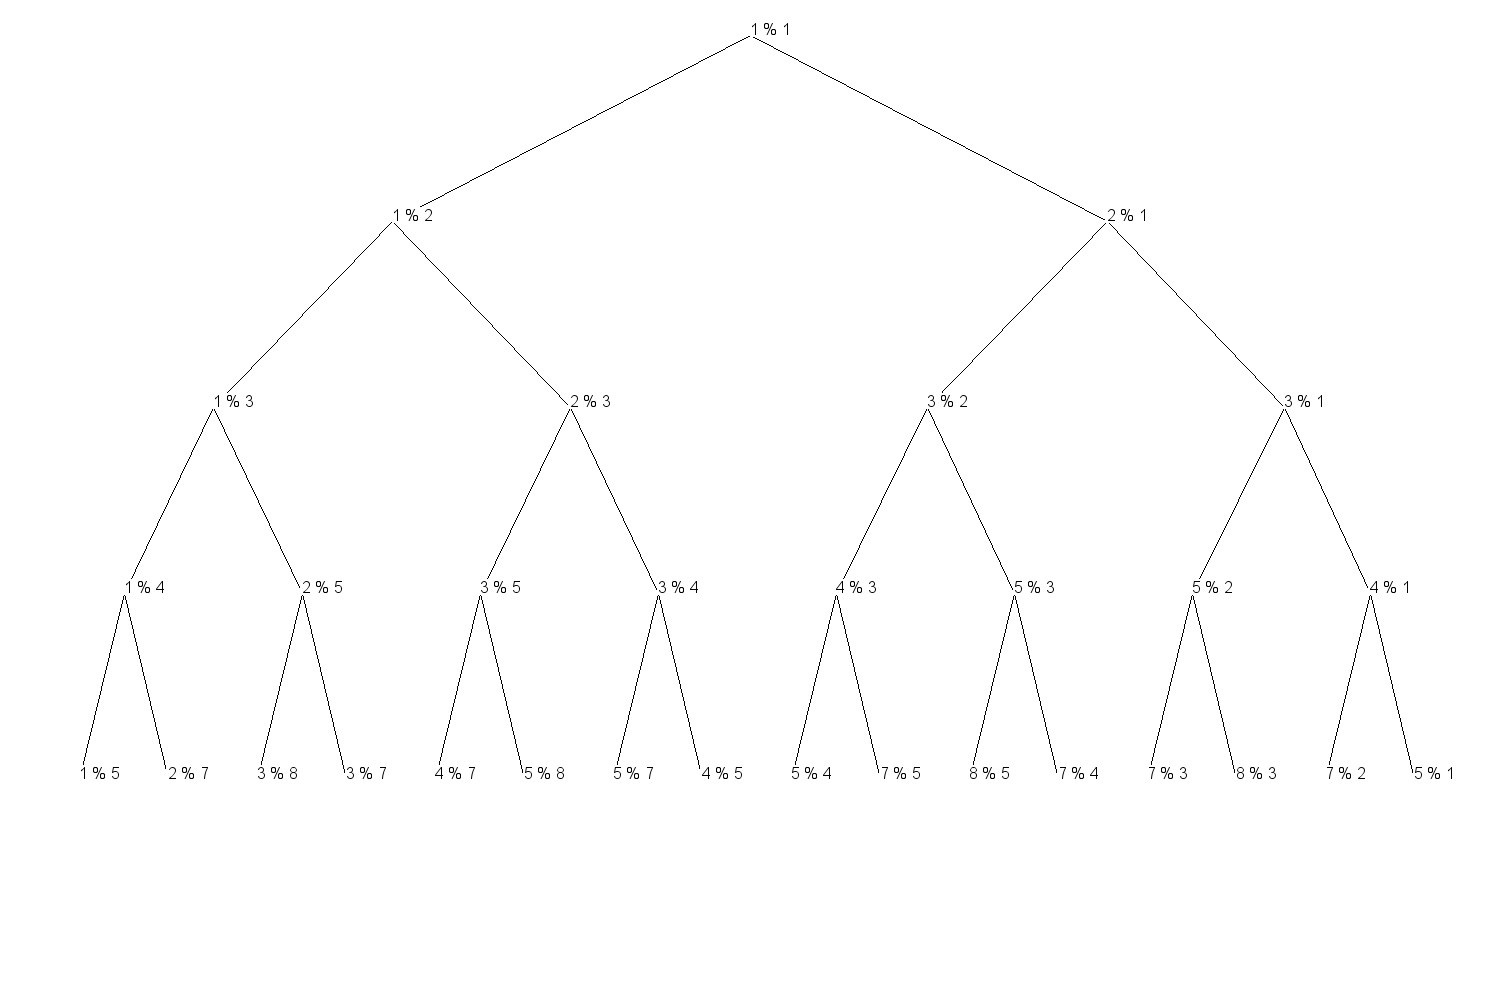
\includegraphics[width=\textwidth]{src/c06/sterb7}
%\end{center}

As you can see at once, this tree has many properties
in common with the Calkin-Wilf tree.
First and trivially, the left kid of a node $k$ is less
than $k$ and the right kid of the same node is greater than $k$.
The left-most branch of the tree contains all fractions
with 1 in the numerator like
$\frac{1}{1},
 \frac{1}{2},
 \frac{1}{3},
 \frac{1}{4}$ and so on.
The right-most branch contains the integers 
$\frac{1}{1},
 \frac{2}{1},
 \frac{3}{1},
 \frac{4}{1}$ and so on.

Furthermore, the product of each generation is 1.
For instance,
$\frac{1}{1} = 1$,
$\frac{1}{2} \times \frac{2}{1} = 1$,
$\frac{1}{3} \times \frac{2}{3} \times
 \frac{3}{2} \times \frac{3}{1} = 1$ and so on.
In fact, we see in each generation the same fractions
we would also see in the Calkin-Wilf tree.
The order of the fraction, however, is different.
More precisely, the order of the inner fractions
differs, since, as we have seen, 
the left-most and right-most numbers are the same.

We could hence ask the obvious question:
how can we permute the generations of the Stern-Brocot tree
to obtain the generations of the Calkin-Wilf tree and vice versa?
Let us look at an example.
The $4^{th}$ generation of the Calkin-Wilf tree is\\
\ensuremath{\Varid{getKids}\;\mathrm{4}\;(\Varid{calWiTree}\;\mathrm{4}\;(\Conid{Q}\;\mathrm{1}\;\mathrm{1}))}: 

\[
\frac{1}{4},
\frac{4}{3},
\frac{3}{5},
\frac{5}{2},
\frac{2}{5},
\frac{5}{3},
\frac{3}{4},
\frac{4}{1}.
\]

The $4^{th}$ generation of the Stern-Brocot tree is\\
\ensuremath{\Varid{getKids}\;\mathrm{4}\;(\Varid{sterbroctree}\;\mathrm{4})}: 

\[
\frac{1}{4},
\frac{2}{5},
\frac{3}{5},
\frac{3}{4},
\frac{4}{3},
\frac{5}{3},
\frac{5}{2},
\frac{4}{1}.
\]

We see that only some fractions changed their place
and the changes are all direct swaps, such that
the second position in the Calkin-Wilf tree changed with
the fifth position and
the fourth position changed with the seventh position.
The other position, the first, third, sixth and eighth,
remain in their place. We could describe this in 
cyclic notation, using indexes from 0 -- 7 
for the eight positions:

\[
(1,4)(3,6).
\]

In other words,
we represent the generations as arrays with indexes 0 -- 7:

\begin{center}
\begingroup
\renewcommand{\arraystretch}{1.5}
\begin{tabular}{|c|c|c|c|c|c|c|c|}\hline
0             & 1             & 2             & 3             & 4             & 5             & 6             & 7 \\\hline\hline
$\frac{1}{4}$ & $\frac{4}{3}$ & $\frac{3}{5}$ & $\frac{5}{2}$ & $\frac{2}{5}$ & $\frac{5}{3}$ & $\frac{3}{4}$ & $\frac{4}{1}$\\\hline
$\frac{1}{4}$ & $\frac{2}{5}$ & $\frac{3}{5}$ & $\frac{3}{4}$ & $\frac{4}{3}$ & $\frac{5}{3}$ & $\frac{5}{2}$ & $\frac{4}{1}$\\\hline
\end{tabular}
\endgroup
\end{center}

So, what is so special about the indexes 1, 3, 4 and 6
that distinguishes them from the indexes 0, 2, 5 and 7?
When we represent these numbers in binary format with
leading zeros, so that all binary numbers have the same length, we have

\begin{center}
\begin{tabular}{|c|c|c|c|c|c|c|c|}\hline
0    & 1   & 2    & 3   & 4   & 5   & 6   & 7 \\\hline\hline
000  & 001 & 010  & 011 & 100 & 101 & 110 & 111\\\hline
\end{tabular}
\end{center}

When we look at the indexes whose fractions do not change,
we see one property that they all have in common:
they are all symmetric. That is, when we reverse the bit strings,
we still have the same number.
$0 = 000$ reversed is still $000 = 0$;
$2 = 010$ reversed is still $010 = 2$;
$5 = 101$ reversed is still $101 = 5$ and
$7 = 111$ reversed is still $111 = 7$.
$1 = 001$ reversed, however, is $100 = 4$ and vice versa and
$3 = 011$ reversed is $110 = 6$.
This corresponds exactly 
to the permutation $(1,4)(3,6)$
and is an instance of a bit-reversal permutation.

Let us try to implement the bit-reversal permutation.
First we implement the bit-reverse of the indexes.
To do so, we first need to convert the decimal index
into a binary number; then we add zeros in front of all
binary numbers that are shorter, in terms of a string
of digits, than the greatest number; then we simply
reverse the lists of binary digits, remove the leading
zeros and convert back to decimal numbers.
This can be nicely expressed by the function

\begin{minipage}{\textwidth}
\begingroup\par\noindent\advance\leftskip\mathindent\(
\begin{pboxed}\SaveRestoreHook
\column{B}{@{}>{\hspre}l<{\hspost}@{}}%
\column{3}{@{}>{\hspre}l<{\hspost}@{}}%
\column{E}{@{}>{\hspre}l<{\hspost}@{}}%
\>[3]{}\Varid{bitrev}\mathbin{::}\Conid{Int}\to [\mskip1.5mu \Conid{Int}\mskip1.5mu]\to [\mskip1.5mu \Conid{Int}\mskip1.5mu]{}\<[E]%
\\
\>[3]{}\Varid{bitrev}\;\Varid{x}\mathrel{=}\Varid{fromBinary}\mathbin{\circ}\Varid{cleanz}\mathbin{\circ}\Varid{reverse}\mathbin{\circ}\Varid{fillup}\;\Varid{x}\;\mathrm{0}\mathbin{\circ}\Varid{toBinary}{}\<[E]%
\ColumnHook
\end{pboxed}
\)\par\noindent\endgroup\resethooks
\end{minipage}

where \ensuremath{\Varid{fillup}} is defined as

\begin{minipage}{\textwidth}
\begingroup\par\noindent\advance\leftskip\mathindent\(
\begin{pboxed}\SaveRestoreHook
\column{B}{@{}>{\hspre}l<{\hspost}@{}}%
\column{3}{@{}>{\hspre}l<{\hspost}@{}}%
\column{18}{@{}>{\hspre}c<{\hspost}@{}}%
\column{18E}{@{}l@{}}%
\column{21}{@{}>{\hspre}l<{\hspost}@{}}%
\column{37}{@{}>{\hspre}l<{\hspost}@{}}%
\column{E}{@{}>{\hspre}l<{\hspost}@{}}%
\>[3]{}\Varid{fillup}\mathbin{::}\Conid{Int}\to \Conid{Int}\to [\mskip1.5mu \Conid{Int}\mskip1.5mu]\to [\mskip1.5mu \Conid{Int}\mskip1.5mu]{}\<[E]%
\\
\>[3]{}\Varid{fillup}\;\Varid{i}\;\Varid{z}\;\Varid{is}{}\<[18]%
\>[18]{}\mid {}\<[18E]%
\>[21]{}\Varid{length}\;\Varid{is}\equiv \Varid{i}{}\<[37]%
\>[37]{}\mathrel{=}\Varid{is}{}\<[E]%
\\
\>[18]{}\mid {}\<[18E]%
\>[21]{}\Varid{otherwise}{}\<[37]%
\>[37]{}\mathrel{=}\Varid{fillup}\;\Varid{i}\;\Varid{z}\;(\Varid{z}\mathbin{:}\Varid{is}){}\<[E]%
\ColumnHook
\end{pboxed}
\)\par\noindent\endgroup\resethooks
\end{minipage}

and \ensuremath{\Varid{cleanz}} as 

\begin{minipage}{\textwidth}
\begingroup\par\noindent\advance\leftskip\mathindent\(
\begin{pboxed}\SaveRestoreHook
\column{B}{@{}>{\hspre}l<{\hspost}@{}}%
\column{3}{@{}>{\hspre}l<{\hspost}@{}}%
\column{18}{@{}>{\hspre}l<{\hspost}@{}}%
\column{E}{@{}>{\hspre}l<{\hspost}@{}}%
\>[3]{}\Varid{cleanz}\mathbin{::}[\mskip1.5mu \Conid{Int}\mskip1.5mu]\to [\mskip1.5mu \Conid{Int}\mskip1.5mu]{}\<[E]%
\\
\>[3]{}\Varid{cleanz}\;[\mskip1.5mu \mskip1.5mu]{}\<[18]%
\>[18]{}\mathrel{=}[\mskip1.5mu \mskip1.5mu]{}\<[E]%
\\
\>[3]{}\Varid{cleanz}\;[\mskip1.5mu \mathrm{0}\mskip1.5mu]{}\<[18]%
\>[18]{}\mathrel{=}[\mskip1.5mu \mathrm{0}\mskip1.5mu]{}\<[E]%
\\
\>[3]{}\Varid{cleanz}\;(\mathrm{0}\mathbin{:}\Varid{is}){}\<[18]%
\>[18]{}\mathrel{=}\Varid{cleanz}\;\Varid{is}{}\<[E]%
\\
\>[3]{}\Varid{cleanz}\;\Varid{is}{}\<[18]%
\>[18]{}\mathrel{=}\Varid{is}{}\<[E]%
\ColumnHook
\end{pboxed}
\)\par\noindent\endgroup\resethooks
\end{minipage}

To apply this, we first have to calculate
the size of the greatest number in our set
in binary format. If we assume that we have
a list of consecutive numbers from $0\dots n-1$,
then the size of the greatest number is just
$\log_2 n$, the binary logarithm of $n$.
For $n=8$, for instance, this is 3.
With this out of the way, we can define
a bit reversal of the indexes of any set \ensuremath{[\mskip1.5mu \Varid{a}\mskip1.5mu]} as:

\begin{minipage}{\textwidth}
\begingroup\par\noindent\advance\leftskip\mathindent\(
\begin{pboxed}\SaveRestoreHook
\column{B}{@{}>{\hspre}l<{\hspost}@{}}%
\column{3}{@{}>{\hspre}l<{\hspost}@{}}%
\column{19}{@{}>{\hspre}l<{\hspost}@{}}%
\column{23}{@{}>{\hspre}l<{\hspost}@{}}%
\column{24}{@{}>{\hspre}l<{\hspost}@{}}%
\column{27}{@{}>{\hspre}l<{\hspost}@{}}%
\column{E}{@{}>{\hspre}l<{\hspost}@{}}%
\>[3]{}\Varid{idxbitrev}\mathbin{::}[\mskip1.5mu \Varid{a}\mskip1.5mu]\to [\mskip1.5mu \Conid{Int}\mskip1.5mu]{}\<[E]%
\\
\>[3]{}\Varid{idxbitrev}\;\Varid{xs}\mathrel{=}{}\<[19]%
\>[19]{}\mathbf{let}\;{}\<[24]%
\>[24]{}\Varid{l}{}\<[27]%
\>[27]{}\mathrel{=}\Varid{length}\;\Varid{xs}{}\<[E]%
\\
\>[24]{}\Varid{x}{}\<[27]%
\>[27]{}\mathrel{=}\Varid{round}\mathbin{\$}\Varid{logBase}\;\mathrm{2}\;(\Varid{fromIntegral}\;\Varid{l}){}\<[E]%
\\
\>[19]{}\mathbf{in}\;{}\<[23]%
\>[23]{}[\mskip1.5mu \Varid{bitrev}\;\Varid{x}\;\Varid{i}\mid \Varid{i}\leftarrow [\mskip1.5mu \mathrm{0}\mathinner{\ldotp\ldotp}\Varid{l}\mathbin{-}\mathrm{1}\mskip1.5mu]\mskip1.5mu]{}\<[E]%
\ColumnHook
\end{pboxed}
\)\par\noindent\endgroup\resethooks
\end{minipage}

and use this function to permute the original input list:

\begin{minipage}{\textwidth}
\begingroup\par\noindent\advance\leftskip\mathindent\(
\begin{pboxed}\SaveRestoreHook
\column{B}{@{}>{\hspre}l<{\hspost}@{}}%
\column{3}{@{}>{\hspre}l<{\hspost}@{}}%
\column{5}{@{}>{\hspre}l<{\hspost}@{}}%
\column{12}{@{}>{\hspre}l<{\hspost}@{}}%
\column{26}{@{}>{\hspre}l<{\hspost}@{}}%
\column{E}{@{}>{\hspre}l<{\hspost}@{}}%
\>[3]{}\Varid{bitreverse}\mathbin{::}[\mskip1.5mu \Varid{a}\mskip1.5mu]\to [\mskip1.5mu \Varid{a}\mskip1.5mu]{}\<[E]%
\\
\>[3]{}\Varid{bitreverse}\;\Varid{xs}\mathrel{=}\Varid{go}\;\Varid{xs}\;(\Varid{idxbitrev}\;\Varid{xs}){}\<[E]%
\\
\>[3]{}\hsindent{2}{}\<[5]%
\>[5]{}\mathbf{where}\;{}\<[12]%
\>[12]{}\Varid{go}\;\anonymous \;[\mskip1.5mu \mskip1.5mu]{}\<[26]%
\>[26]{}\mathrel{=}[\mskip1.5mu \mskip1.5mu]{}\<[E]%
\\
\>[12]{}\Varid{go}\;\Varid{zs}\;(\Varid{p}\mathbin{:}\Varid{ps}){}\<[26]%
\>[26]{}\mathrel{=}\Varid{zs}\mathbin{!!}\Varid{p}\mathbin{:}\Varid{go}\;\Varid{zs}\;\Varid{ps}{}\<[E]%
\ColumnHook
\end{pboxed}
\)\par\noindent\endgroup\resethooks
\end{minipage}

Applied on the list \ensuremath{[\mskip1.5mu \mathrm{0},\mathrm{1},\mathrm{2},\mathrm{3},\mathrm{4},\mathrm{5},\mathrm{6}\mskip1.5mu]},
we see exactly the $(1,4)(3,6)$ permutation
we saw above, namely \ensuremath{[\mskip1.5mu \mathrm{0},\mathrm{4},\mathrm{2},\mathrm{6},\mathrm{1},\mathrm{5},\mathrm{3}\mskip1.5mu]}.
Applied on a generation from the Calkin-Wilf tree,
we see the corresponding generation from the 
Stern-Brocot tree. 
Let \ensuremath{\Varid{t}\mathrel{=}\Varid{calWiTree}\;(\mathbin{-}\mathrm{1})\;(\mathrm{1}\mathbin{\%}\mathrm{1})},
we see for 

\begin{center}
\begingroup
\renewcommand{\arraystretch}{1.5}
\begin{tabular}{|c|c|}\hline
\ensuremath{\Varid{getKids}\;\mathrm{3}\;\Varid{t}} & 
$\frac{1}{3},
 \frac{3}{2},
 \frac{2}{3},
 \frac{3}{1}$ \\\hline
\ensuremath{\Varid{bitreverse}\;(\Varid{getKids}\;\mathrm{3}\;\Varid{t})} &
$\frac{1}{3},
 \frac{2}{3},
 \frac{3}{2},
 \frac{3}{1}$\\\hline
\ensuremath{\Varid{getKids}\;\mathrm{4}\;\Varid{t}} & 
$\frac{1}{4},
 \frac{4}{3},
 \frac{3}{5},
 \frac{5}{2},
 \frac{2}{5},
 \frac{5}{3},
 \frac{3}{4}, 
 \frac{4}{1}$ \\\hline
\ensuremath{\Varid{bitreverse}\;(\Varid{getKids}\;\mathrm{4}\;\Varid{t})} &
$\frac{1}{4},
 \frac{2}{5},
 \frac{3}{5},
 \frac{3}{4},
 \frac{4}{3},
 \frac{5}{3},
 \frac{5}{2},
 \frac{4}{1}$\\\hline
\end{tabular}
\endgroup
\end{center}

Since the generations of the Stern-Brocot tree
are nothing but permutations of the Calkin-Wilf tree, we
obviously, can derive a sequence from the Stern-Brocot tree
that lists all rational numbers.
We create this sequence in exaclty the same way
we did for the CalkinWilf tree, namely

\begin{minipage}{\textwidth}
\begingroup\par\noindent\advance\leftskip\mathindent\(
\begin{pboxed}\SaveRestoreHook
\column{B}{@{}>{\hspre}l<{\hspost}@{}}%
\column{3}{@{}>{\hspre}l<{\hspost}@{}}%
\column{5}{@{}>{\hspre}l<{\hspost}@{}}%
\column{E}{@{}>{\hspre}l<{\hspost}@{}}%
\>[3]{}\Varid{enumQsb}\mathbin{::}[\mskip1.5mu \Conid{Quoz}\mskip1.5mu]{}\<[E]%
\\
\>[3]{}\Varid{enumQsb}\mathrel{=}\Varid{go}\;\mathrm{1}\mathbin{\$}\Varid{sterbrocTree}\;(\mathbin{-}\mathrm{1}){}\<[E]%
\\
\>[3]{}\hsindent{2}{}\<[5]%
\>[5]{}\mathbf{where}\;\Varid{go}\;\Varid{i}\;\Varid{t}\mathrel{=}\Varid{getKids}\;\Varid{i}\;\Varid{t}\plus \Varid{go}\;(\Varid{i}\mathbin{+}\mathrm{1})\;\Varid{t}{}\<[E]%
\ColumnHook
\end{pboxed}
\)\par\noindent\endgroup\resethooks
\end{minipage}\ignore{$}

The numerators of the sequence derived in this way
from the Calkin-Wilf tree equal the well-known Stern sequence.
Is there another well-known sequence that is equivalent
to the numerators of the Stern-Brocot tree sequence?
Let us ask the On-line Encyclopedy with the first segment
of that sequence generated by \ensuremath{\Varid{map}\;\Varid{numerator}\;(\Varid{take}\;\mathrm{20}\;\Varid{enumQsb})}:

\[
1,1,2,1,2,3,3,1,2,3,3,4,5,5,4,1,2,3,3,4,5,5,4,5,7.
\]

The Encyclopedy tells us that this is the numerators of
the \term{Farey sequence}.
This sequence, named for British geologist 
John Farey (1766 -- 1826), has a lot of remarkable properties.
The Farey sequence of $n$ lists all fractions 
in canoncial form between 0 and 1,
usually included, with a denominator less or equal than $n$.
For instance, the Farey sequence of 1, designated $F_1$ just contains
$0,1$; $F_2$ contains $0,\frac{1}{2},1$;
$F_3$ contains $0,\frac{1}{3},\frac{2}{3},1$ and so on.

A direct way to implement this could be to combine all numbers
from $0\dots n$ in the numerator with all numbers $1\dots n$
in the denominator that are smaller 1 and to sort and \ensuremath{\Varid{nub}}
the resulting list, like this:

\begin{minipage}{\textwidth}
\begingroup\par\noindent\advance\leftskip\mathindent\(
\begin{pboxed}\SaveRestoreHook
\column{B}{@{}>{\hspre}l<{\hspost}@{}}%
\column{3}{@{}>{\hspre}l<{\hspost}@{}}%
\column{27}{@{}>{\hspre}l<{\hspost}@{}}%
\column{E}{@{}>{\hspre}l<{\hspost}@{}}%
\>[3]{}\Varid{farey2}\mathbin{::}\Conid{Natural}\to [\mskip1.5mu \Conid{Quoz}\mskip1.5mu]{}\<[E]%
\\
\>[3]{}\Varid{farey2}\;\Varid{n}\mathrel{=}\Varid{sort}\;(\Varid{nub}\mathbin{\$}{}\<[27]%
\>[27]{}\Varid{filter}\;(\leq \mathrm{1})\mathbin{\$}{}\<[E]%
\\
\>[27]{}\Varid{concatMap}\;(\lambda \Varid{x}\to \Varid{map}\;(\Varid{x}\mathbin{\%})\;[\mskip1.5mu \mathrm{1}\mathinner{\ldotp\ldotp}\Varid{n}\mskip1.5mu])\;[\mskip1.5mu \mathrm{0}\mathinner{\ldotp\ldotp}\Varid{n}\mskip1.5mu]){}\<[E]%
\ColumnHook
\end{pboxed}
\)\par\noindent\endgroup\resethooks
\end{minipage}

With this approach, we create a lot of fractions
that we do not need and that we filter out again afterwards.
A more interesting approach, also in the light of the topic
of this section, is the following:

\begin{minipage}{\textwidth}
\begingroup\par\noindent\advance\leftskip\mathindent\(
\begin{pboxed}\SaveRestoreHook
\column{B}{@{}>{\hspre}l<{\hspost}@{}}%
\column{3}{@{}>{\hspre}l<{\hspost}@{}}%
\column{5}{@{}>{\hspre}l<{\hspost}@{}}%
\column{12}{@{}>{\hspre}l<{\hspost}@{}}%
\column{20}{@{}>{\hspre}c<{\hspost}@{}}%
\column{20E}{@{}l@{}}%
\column{23}{@{}>{\hspre}l<{\hspost}@{}}%
\column{28}{@{}>{\hspre}l<{\hspost}@{}}%
\column{E}{@{}>{\hspre}l<{\hspost}@{}}%
\>[3]{}\Varid{farey}\mathbin{::}\Conid{Natural}\to [\mskip1.5mu \Conid{Quoz}\mskip1.5mu]{}\<[E]%
\\
\>[3]{}\Varid{farey}\;\Varid{n}\mathrel{=}\mathrm{0}\mathbin{\%}\mathrm{1}\mathbin{:}\Varid{sort}\;(\Varid{go}\;\mathrm{1}\mathbin{\$}\Varid{sterbrocTree}\;(\mathbin{-}\mathrm{1})){}\<[E]%
\\
\>[3]{}\hsindent{2}{}\<[5]%
\>[5]{}\mathbf{where}\;{}\<[12]%
\>[12]{}\Varid{go}\;\Varid{k}\;\Varid{t}{}\<[20]%
\>[20]{}\mathrel{=}{}\<[20E]%
\>[23]{}\mathbf{let}\;{}\<[28]%
\>[28]{}\Varid{g}\mathrel{=}\Varid{getKids}\;\Varid{k}\;\Varid{t}{}\<[E]%
\\
\>[28]{}\Varid{l}\mathrel{=}\Varid{filter}\;\Varid{fltr}\;\Varid{g}{}\<[E]%
\\
\>[23]{}\mathbf{in}\;\mathbf{if}\;\Varid{null}\;\Varid{l}\;\mathbf{then}\;\Varid{l}\;\mathbf{else}\;\Varid{l}\plus \Varid{go}\;(\Varid{k}\mathbin{+}\mathrm{1})\;\Varid{t}{}\<[E]%
\\
\>[12]{}\Varid{fltr}\;\Varid{k}{}\<[20]%
\>[20]{}\mathrel{=}{}\<[20E]%
\>[23]{}\Varid{k}\leq \mathrm{1}\mathrel{\wedge}\Varid{n}\geq \Varid{denominator}\;\Varid{k}{}\<[E]%
\ColumnHook
\end{pboxed}
\)\par\noindent\endgroup\resethooks
\end{minipage}

Here, we iterate over the generations of the Stern-Brocot tree
removing the fractions that are greater 1 or have a denominator
greater n. When we do not get results anymore, \ie\ all denominators
are greater $n$, we are done.

Let us try this algorithm on some numbers:

\begin{equation}
F_4 = \left\lbrace 0, 
\frac{1}{4}, 
\frac{1}{3}, 
\frac{1}{2}, 
\frac{2}{3}, 
\frac{3}{4}, 
1\right\rbrace
\end{equation}
\begin{equation}
F_5 = \left\lbrace 0, 
\frac{1}{5}, 
\frac{1}{4}, 
\frac{1}{3}, 
\frac{2}{5}, 
\frac{1}{2}, 
\frac{3}{5}, 
\frac{2}{3}, 
\frac{3}{4}, 
\frac{4}{5}, 
1\right\rbrace
\end{equation}
\begin{equation}
F_6 = \left\lbrace 0, 
\frac{1}{6}, 
\frac{1}{5}, 
\frac{1}{4}, 
\frac{1}{3}, 
\frac{2}{5}, 
\frac{1}{2}, 
\frac{3}{5}, 
\frac{2}{3}, 
\frac{3}{4}, 
\frac{4}{5}, 
\frac{5}{6}, 
1\right\rbrace
\end{equation}

We see some interesting properties.
First and this should be obvious,
we see $n$ as a denominator in sequence $F_n$ exaclty
$\varphi(n)$ times.
For $F_6$, for instance, we could create the fractions
$\frac{1}{6}$, 
$\frac{2}{6}$, 
$\frac{3}{6}$, 
$\frac{4}{6}$ and
$\frac{5}{6}$.
The fractions $\frac{2}{6}\dots\frac{4}{6}$, however,
are not in canonical form, since the numerators $2\dots 4$ 
all share divisors with 6. Therefore, only those fractions
remain for which the numerator does not share divisors
whith $n$. There are, as we know, $\varphi(n)$ such numerators.

Another property is that, for two consecutive fractions,
$\frac{a}{b}$ and $\frac{c}{d}$,
in a Farey sequence, the cross products
$ad$ and $cb$ are consecutive integers.
In again $F_6$, 
for the fractions $\frac{1}{6}$ and $\frac{1}{5}$,
the cross products, trivially, are 5 and 6.
More interesting are 
the fractions $\frac{3}{5}$ and $\frac{2}{3}$ whose
cross products are $3\times 3 = 9$ and $5 \times 2 = 10$.

Even further, for any three consecutive fractions
in a Farey sequence, the middle one, called the mediant fraction,
can be calculated from the outer ones as
$\frac{a}{b}, \frac{a+c}{b+d}, \frac{c}{d}$.
For instance in $F_6$: 

\begin{equation}
 \frac{1+1}{6+4} = \frac{2}{10} = \frac{1}{5},
\end{equation}
\begin{equation}
 \frac{2+3}{5+5} = \frac{5}{10} = \frac{1}{2}
\end{equation}
and
\begin{equation}
 \frac{3+5}{4+6} = \frac{8}{10} = \frac{4}{5}.
\end{equation}

This property can be used to compute $F_{n+1}$ from $F_n$.
We just have to insert those mediant fractions 
of two consecutive fractions in $F_n$, for which
the denominator is $n+1$.
In $F_6$ we would insert

\[
\frac{0+1}{1+6},
\frac{1+1}{4+3},
\frac{2+1}{5+2},
\frac{1+3}{2+5},
\frac{2+3}{3+4},
\frac{5+1}{6+1}
\]

resulting in

\begin{equation}
F_7 = \left\lbrace 0, 
\frac{1}{7}, 
\frac{1}{6}, 
\frac{1}{5}, 
\frac{1}{4}, 
\frac{2}{7}, 
\frac{1}{3}, 
\frac{2}{5}, 
\frac{3}{7}, 
\frac{1}{2}, 
\frac{4}{7}, 
\frac{3}{5}, 
\frac{2}{3}, 
\frac{5}{7}, 
\frac{3}{4}, 
\frac{4}{5}, 
\frac{5}{6}, 
\frac{6}{7}, 
1\right\rbrace
\end{equation}

We can implement this as

\begin{minipage}{\textwidth}
\begingroup\par\noindent\advance\leftskip\mathindent\(
\begin{pboxed}\SaveRestoreHook
\column{B}{@{}>{\hspre}l<{\hspost}@{}}%
\column{3}{@{}>{\hspre}l<{\hspost}@{}}%
\column{5}{@{}>{\hspre}l<{\hspost}@{}}%
\column{16}{@{}>{\hspre}l<{\hspost}@{}}%
\column{19}{@{}>{\hspre}l<{\hspost}@{}}%
\column{20}{@{}>{\hspre}l<{\hspost}@{}}%
\column{21}{@{}>{\hspre}l<{\hspost}@{}}%
\column{24}{@{}>{\hspre}c<{\hspost}@{}}%
\column{24E}{@{}l@{}}%
\column{27}{@{}>{\hspre}l<{\hspost}@{}}%
\column{47}{@{}>{\hspre}l<{\hspost}@{}}%
\column{E}{@{}>{\hspre}l<{\hspost}@{}}%
\>[3]{}\Varid{nxtFarey}\mathbin{::}\Conid{Natural}\to [\mskip1.5mu \Conid{Quoz}\mskip1.5mu]\to [\mskip1.5mu \Conid{Quoz}\mskip1.5mu]{}\<[E]%
\\
\>[3]{}\Varid{nxtFarey}\;\Varid{n}\;[\mskip1.5mu \mskip1.5mu]{}\<[19]%
\>[19]{}\mathrel{=}[\mskip1.5mu \mskip1.5mu]{}\<[E]%
\\
\>[3]{}\Varid{nxtFarey}\;\Varid{n}\;[\mskip1.5mu \Varid{r}\mskip1.5mu]{}\<[19]%
\>[19]{}\mathrel{=}[\mskip1.5mu \Varid{r}\mskip1.5mu]{}\<[E]%
\\
\>[3]{}\Varid{nxtFarey}\;\Varid{n}\;(\Varid{a}\mathbin{:}\Varid{b}\mathbin{:}\Varid{rs}){}\<[24]%
\>[24]{}\mid {}\<[24E]%
\>[27]{}\Varid{denominator}\;\Varid{a}\mathbin{+}{}\<[E]%
\\
\>[27]{}\Varid{denominator}\;\Varid{b}\equiv \Varid{n}{}\<[47]%
\>[47]{}\mathrel{=}\Varid{nxtFarey}\;\Varid{n}\;(\Varid{a}\mathbin{:}\Varid{x}\mathbin{:}\Varid{b}\mathbin{:}\Varid{rs}){}\<[E]%
\\
\>[24]{}\mid {}\<[24E]%
\>[27]{}\Varid{otherwise}{}\<[47]%
\>[47]{}\mathrel{=}\Varid{a}\mathbin{:}\Varid{nxtFarey}\;\Varid{n}\;(\Varid{b}\mathbin{:}\Varid{rs}){}\<[E]%
\\
\>[3]{}\hsindent{2}{}\<[5]%
\>[5]{}\mathbf{where}\;\Varid{x}\mathrel{=}{}\<[16]%
\>[16]{}\mathbf{let}\;{}\<[21]%
\>[21]{}\Varid{n1}\mathrel{=}\Varid{numerator}\;\Varid{a}{}\<[E]%
\\
\>[21]{}\Varid{n2}\mathrel{=}\Varid{numerator}\;\Varid{b}{}\<[E]%
\\
\>[21]{}\Varid{d1}\mathrel{=}\Varid{denominator}\;\Varid{a}{}\<[E]%
\\
\>[21]{}\Varid{d2}\mathrel{=}\Varid{denominator}\;\Varid{b}{}\<[E]%
\\
\>[16]{}\mathbf{in}\;{}\<[20]%
\>[20]{}(\Varid{n1}\mathbin{+}\Varid{n2})\mathbin{\%}(\Varid{d1}\mathbin{+}\Varid{d2}){}\<[E]%
\ColumnHook
\end{pboxed}
\)\par\noindent\endgroup\resethooks
\end{minipage}
 
In fact, we can construct the Stern-Brocot tree
by means of mediant fractions. The outer fractions,
in this algorithm are the predecessors of the current node,
namely the direct predecessor and either the predecessor
of the predecessor or the sibling of that node.
For instace, the second node in the third generation
is $\frac{2}{3}$. Its kids are 
$\frac{3}{5}$ and $\frac{3}{4}$.
$\frac{3}{5}$ is $\frac{2+1}{3+2}$;
$\frac{4}{3}$, however, is $\frac{2+1}{3+1}$
and, hence, the predecessor of the predecessor
of $\frac{2}{3}$.

The question now is how to bootstrap this algorithm.
The root node, of course, does not have predecessors.
For this case, we imagine two predecessors, namely
the fractions $\frac{0}{1}$ and $\frac{1}{0}$,
the latter of which, of course, is not a proper fraction.
The assumption of such nodes, however, helps us derive
the outer branches, where, on the left side, the numerator
does not change, hence is constructed by addition with 0, and,
on the right side, the denominator does not change and is
likewise constructed by addition with 0.

We implement this as

\begin{minipage}{\textwidth}
\begingroup\par\noindent\advance\leftskip\mathindent\(
\begin{pboxed}\SaveRestoreHook
\column{B}{@{}>{\hspre}l<{\hspost}@{}}%
\column{3}{@{}>{\hspre}l<{\hspost}@{}}%
\column{29}{@{}>{\hspre}l<{\hspost}@{}}%
\column{30}{@{}>{\hspre}c<{\hspost}@{}}%
\column{30E}{@{}l@{}}%
\column{33}{@{}>{\hspre}l<{\hspost}@{}}%
\column{38}{@{}>{\hspre}l<{\hspost}@{}}%
\column{42}{@{}>{\hspre}l<{\hspost}@{}}%
\column{44}{@{}>{\hspre}l<{\hspost}@{}}%
\column{54}{@{}>{\hspre}l<{\hspost}@{}}%
\column{E}{@{}>{\hspre}l<{\hspost}@{}}%
\>[3]{}\Varid{mSterbroctree}\mathbin{::}\Conid{Zahl}\to {}\<[29]%
\>[29]{}\Conid{Natural}\to \Conid{Natural}\to {}\<[E]%
\\
\>[29]{}\Conid{Natural}\to \Conid{Natural}\to \Conid{Quoz}\to \Conid{Tree}\;\Conid{Quoz}{}\<[E]%
\\
\>[3]{}\Varid{mSterbroctree}\;\mathrm{0}\;\anonymous \;\anonymous \;\anonymous \;\anonymous \;\Varid{r}{}\<[30]%
\>[30]{}\mathrel{=}{}\<[30E]%
\>[33]{}\Conid{Node}\;\Varid{r}\;[\mskip1.5mu \mskip1.5mu]{}\<[E]%
\\
\>[3]{}\Varid{mSterbroctree}\;\Varid{n}\;\Varid{a}\;\Varid{b}\;\Varid{c}\;\Varid{d}\;\Varid{r}{}\<[30]%
\>[30]{}\mathrel{=}{}\<[30E]%
\>[33]{}\mathbf{let}\;{}\<[38]%
\>[38]{}\Varid{rn}{}\<[42]%
\>[42]{}\mathrel{=}\Varid{numerator}\;\Varid{r}{}\<[E]%
\\
\>[38]{}\Varid{rd}{}\<[42]%
\>[42]{}\mathrel{=}\Varid{denominator}\;\Varid{r}{}\<[E]%
\\
\>[38]{}\Varid{k1}{}\<[42]%
\>[42]{}\mathrel{=}(\Varid{a}\mathbin{+}\Varid{rn})\mathbin{\%}(\Varid{b}\mathbin{+}\Varid{rd}){}\<[E]%
\\
\>[38]{}\Varid{k2}{}\<[42]%
\>[42]{}\mathrel{=}(\Varid{c}\mathbin{+}\Varid{rn})\mathbin{\%}(\Varid{d}\mathbin{+}\Varid{rd}){}\<[E]%
\\
\>[33]{}\mathbf{in}\;{}\<[38]%
\>[38]{}\mathbf{if}\;\Varid{k1}\mathbin{<}\Varid{k2}{}\<[E]%
\\
\>[38]{}\mathbf{then}\;{}\<[44]%
\>[44]{}\Conid{Node}\;\Varid{r}\;[\mskip1.5mu {}\<[54]%
\>[54]{}\Varid{mSterbroctree}\;(\Varid{n}\mathbin{-}\mathrm{1})\;\Varid{a}\;\Varid{b}\;\Varid{rn}\;\Varid{rd}\;\Varid{k1},{}\<[E]%
\\
\>[54]{}\Varid{mSterbroctree}\;(\Varid{n}\mathbin{-}\mathrm{1})\;\Varid{c}\;\Varid{d}\;\Varid{rn}\;\Varid{rd}\;\Varid{k2}\mskip1.5mu]{}\<[E]%
\\
\>[38]{}\mathbf{else}\;{}\<[44]%
\>[44]{}\Conid{Node}\;\Varid{r}\;[\mskip1.5mu {}\<[54]%
\>[54]{}\Varid{mSterbroctree}\;(\Varid{n}\mathbin{-}\mathrm{1})\;\Varid{c}\;\Varid{d}\;\Varid{rn}\;\Varid{rd}\;\Varid{k2},{}\<[E]%
\\
\>[54]{}\Varid{mSterbroctree}\;(\Varid{n}\mathbin{-}\mathrm{1})\;\Varid{a}\;\Varid{b}\;\Varid{rn}\;\Varid{rd}\;\Varid{k1}\mskip1.5mu]{}\<[E]%
\ColumnHook
\end{pboxed}
\)\par\noindent\endgroup\resethooks
\end{minipage}

Note that we have to use two pairs of natural numbers
instead of two fractions to encode the predecessors.
This is because we have to represent the imagined
predecessor $\frac{1}{0}$, which is not a proper fraction.
Finally, we check for the smaller of the resulting numbers
$k_1$ and $k_2$ to make sure that the smaller one 
always goes to the left and the greater to the right.
This implementation now gives exactly the same tree
as the implementation using continued fractions
introduced at the beginning of the section.

\section{p-adic Numbers} 
\section{Real Factorials}
\section{The Continuum}
\section{Review of the Number Zoo}

% -------------------------------------------------------------------------
\part{Algebra and Geometry}
% -------------------------------------------------------------------------

\chapter{Polynomials} % c07
\section{Numeral Systems}
\section{The Algebra of Polynomials}
\section{Factoring Polynomials}
\section{Polynomials and Binomial Coefficients}
\section{The Method of partial Fractions}
\ignore{
http://www.purplemath.com/modules/partfrac.htm
}
\section{The Difference Engine}
\section{Generationfunctionology 1}
\section{The closed Form of the Fibonacci Sequence}
\ignore{
\begingroup\par\noindent\advance\leftskip\mathindent\(
\begin{pboxed}\SaveRestoreHook
\column{B}{@{}>{\hspre}l<{\hspost}@{}}%
\column{E}{@{}>{\hspre}l<{\hspost}@{}}%
\>[B]{}\mathbf{module}\;\Conid{ClosedFib}{}\<[E]%
\\
\>[B]{}\mathbf{where}{}\<[E]%
\ColumnHook
\end{pboxed}
\)\par\noindent\endgroup\resethooks
}

\begin{equation}
G(x) = F_0 + F_1x + F_2x^2 + F_3x^3 + \dots
\end{equation}

\begin{equation}
G(x) = 0 + x + x^2 + 2x^3 + 3x^4 + 5x^5 + 8x^6 + \dots
\end{equation}

\begin{equation}
xG(x) = F_0x + F_1x^2 + F_2x^3 + F_3x^4 + \dots
\end{equation}

\begin{equation}
x^2G(x) = F_0x^2 + F_1x^3 + F_2x^4 + F_3x^5 + \dots
\end{equation}

\begin{equation}
G(x) - xG(x) - x^2G(x) = (1-x-x^2)G(x).
\end{equation}

\begin{align*}
(1-x-x^2)G(x) & = & (&F_0 & + & F_1x & + & F_2x^2 & + & F_3x^3 & + & \dots) & - \\
              &   & (&    &   & F_0x & + & F_1x^2 & + & F_2x^3 & + & \dots) & - \\
              &   & (&    &   &      & + & F_0x^2 & + & F_1x^3 & + & \dots) &
\end{align*}

\begin{align*}
(1-x-x^2)G(x) & = & F_0 & + (F_1 - F_0)x \\
              &   &     & + (F_2 - F_1 - F_0)x^2 \\
              &   &     & + (F_3 - F_2 - F_1)x^3 \\
              &   &     & + \dots
\end{align*}

\begin{equation}
(1-x-x^2)G(x) = x.
\end{equation}

\begin{equation}
G(x) = \frac{x}{1-x-x^2}.
\end{equation}

\ignore{
- factor denominator using roots:
  - (x+1/2+sqrt(5)/2) 
  - (x+1/2-sqrt(5)/2)
- then use partial fractions
}




\chapter{Relations, Functions and the Cartesian Plane} % c08
\section{Relations}
\section{Equivalence Classes}
\section{Functions}
\section{Visual Functions}
\section{Trigonometry}
\section{Conic Sections}
\section{Algebra and Geometry}

\chapter{Linear Algebra} % c09
\section{Vectors}
\section{Vector Spaces}
\section{Clustering}
\section{Linear Maps and Operators}
\section{The Matrix}
\section{Eigenvalues}
\section{Inner Products and their Operators}
\section{Polynomials and Vector Spaces}
\section{Determinants}
\section{Support Vector Machines}

\chapter{Complex Numbers} % c10
\section{i}
\section{Complex Numbers}
\section{The complex Plane}
\section{Polar Form}
\section{$\mathbb{C}$}
\section{Gaussian Integers}
\section{...}
\section{Complex Vector Spaces}
\section{...}
\section{Quantum Mechanics}
\section{Hypercomplex Numbers}

\chapter{Quadratics, Cubics and Quartics} % c11
\section{Quadratic Equations}
\section{The fundamental Theorem of Algebra}
% see "algebraic proofs" in http://en.wikipedia.org/wiki/Fundamental_theorem_of_algebra
% \section{Non-algebraic Numbers}
\section{Cubics and Quartics}
\section{Quintics}
\section{Galois Theory}
\section{Field Theory}
\section{Category Theory}
% Riemann's Hypothesis?

\chapter{Elliptic Curves} % c12
 

\chapter{Euclid and beyond} % c13
\section{Euclid's Geometry}
\section{The Parallel Postulate}
\section{Non-Euclidian Geometries}
% including Poincaré's disk world
\section{Lost in Hilbert Space}
\section{Geometry and Relativity}
\section{Projective Geometry}
\section{Graph Theory}
\section{Topology}

% -------------------------------------------------------------------------
\part{Analysis}
% -------------------------------------------------------------------------

\chapter{The Calculus} % c14
\section{The Method of Exhaustion}
\section{Area below a Curve}
\section{Basic Rules of Integration}
\section{Minima, Maxima and Slopes}
\section{Basic Rules of Derivation}
\section{The fundamental Theorem of the Calculus}
\section{More Rules}

\chapter{Curve Sketching} % c13
\chapter{Advanced Function Analysis} % c14
\chapter{Generating Functions} % c15
\chapter{Applied Mathematics} % c16
\chapter{Prospects} % c17

\end{document}
